% GRASP: Copyright 1997,1998,1999,2000  Bruce Allen
\def\versionnumber{{\bf GRASP RELEASE 1.9.8}}
% $Id manual.tex,v 1.76 1999/06/25 00:14:01 ballen Exp $
% GRASP USERS MANUAL COPYRIGHT BRUCE ALLEN, 1997, 1998, 1999

% UNCOMMENT TO INCLUDE ONLY ONE OR MORE SECTIONS
% \includeonly{comma-separated file list (with no .tex extensions)}
% \includeonly{man_intro}
% \includeonly{man_correlation}
% \includeonly{man_40meter}
% \includeonly{man_utility}
% \includeonly{man_inspiral}
% \includeonly{man_ringdown}
% \includeonly{man_template}
% \includeonly{man_transient}
% \includeonly{man_binary-search}
% \includeonly{man_stochastic}
% \includeonly{man_frame}
% \includeonly{man_GRtoolbox}
% \includeonly{man_timefrequency}

\makeindex

\documentclass[11pt]{article}
\usepackage{times,epsfig,lgrind}
\usepackage[hypertex,pagebackref=true,letterpaper=true,linkcolor=blue]{hyperref}
\usepackage{fancyhdr}

%define page size
\setlength{\textheight}{9.0in}
\setlength{\textwidth}{6.5in}
\setlength{\topmargin}{-0.25in}
\setlength{\oddsidemargin}{0in}
\setlength{\evensidemargin}{0in}

%set up headers and footers on each page
\pagestyle{fancy}
\fancyhf{}
\lhead{\bf\begin{tabular}{c}Section\\\thesubsection\end{tabular}}
\chead{\bf\leftmark}
\rhead{\bf\begin{tabular}{c}Page\\\thepage\end{tabular}}
\lfoot{\bf\versionnumber}
\cfoot{\bf Page~\thepage}
\rfoot{\bf\today}

% Define marks without the section numbers
\renewcommand{\sectionmark}[1]{\markboth{#1}{}}
\renewcommand{\subsectionmark}[1]{\markright{#1}}

% Make equation numbers reset to zero at start of each subsection
\def\theequation{\thesubsection.\arabic{equation}}
\renewcommand{\refname}{}
\date{\today}
\makeatletter
\@addtoreset{equation}{subsection}
\makeatother
\providecommand{\eth}{\partial\!\!{}^{-}}


% Start the document
\begin{document}

\title{GRASP: a data analysis package for gravitational wave detection}
\author{Bruce Allen\thanks{\tt ballen@dirac.phys.uwm.edu}\\
Department of Physics\\
University of Wisconsin - Milwaukee\\
PO Box 413\\
Milwaukee WI 53201, USA}

\maketitle

\begin{center}
{\bf Contributors:}
\end{center}
Warren Anderson,
R. Balasubramanian,
Kent Blackburn,
Patrick Brady,
Jim Brau,
Jolien Creighton,
Teviet Creighton,
Steve Drasco,
Serge Droz,
Eanna Flanagan,
Wensheng Hua,
Scott Hughes,
Dustin Laurence,
Adrian Ottewill,
Ben Owen,
Jorge Pullin,
Joseph Romano, and
Alan Wiseman.
\vskip 1.0 in

\begin{abstract}
\noindent
GRASP ({\bf G}ravitational {\bf R}adiation {\bf A}nalysis \& {\bf
S}imulation {\bf P}ackage) is a public-domain software tool-kit designed
for analysis and simulation of data from gravitational wave detectors.
This users manual describes the use and features of this package.
Note: an up-to-date version of this manual may be obtained at:
\htmladdnormallink{{\tt http://www.lsc-group.phys.uwm.edu/$\sim$ballen/grasp-distribution/}}
{http://www.lsc-group.phys.uwm.edu/~ballen/grasp-distribution/}.
The software package is also available from this site.
\end{abstract}
\vskip -6.5 in \centerline{\bf USERS MANUAL}
\vskip 7.0 in

\begin{center}
Copyright 1999 \copyright Bruce Allen
\end{center}
\vskip 0.5in
\begin{center}
{\bf \versionnumber}
\end{center}
\clearpage
\chead{\bf TABLE OF CONTENTS }
\lhead{\bf\begin{tabular}{c}Section\\0\end{tabular}}
\tableofcontents
\clearpage
\chead{\bf \leftmark}
\lhead{\bf\begin{tabular}{c}Section\\\thesubsection\end{tabular}}

\section{ACKNOWLEDGEMENTS}
This work has been partially supported by National Science Foundation
grants to: the University of Wisconsin - Milwaukee PHY9507740 and PHY9728704, the
LIGO project PHY9210038 and the LIGO visitors program PHY9603177.
It has also benefited from the contributions of several individuals.
Alan Wiseman wrote the chirp generation routines with me in 1995, then
entirely re-wrote them for GRASP.  Joseph Romano took my (AVS versions of
the) stochastic background code, helped to fix a number of the problems,
and produced the stochastic background simulation routines contained in
GRASP.   Sathyaprakash generously provided me with a copy of his routine
{\tt grid4.f} which eventually evolved into {\tt template\_grid}.  Jolien
Creighton wrote and documented the section on black hole ringdown, and
incorporated the FFTW optimized Fourier transform routines.  
Teviet Creighton, Ben Owen, Scott Hughes and Patrick Brady contributed
essential pieces towards the binary-inspiral search performed on the
Caltech 40-meter data from November 1994. Jim Mason
was ``instrumental" in helping me to understand and document the data
format used in the 40-meter prototype experiment.  Fred Raab, Bob Spero,
Stan Whitcomb, Kent Blackburn and others have contributed many useful
ideas and insights about how to understand the data stream from a real
interferometer.  Kip Thorne and his research group provided or called
attention to many of these ideas.
\clearpage

\chead{\bf\begin{tabular}{c}\leftmark\\\rightmark\end{tabular}}
% GRASP: Copyright 1997,1998,1999  Bruce Allen
% $Id: man_intro.tex,v 1.52 2000/05/19 15:19:52 ballen Exp $
\section{Introduction}
\setcounter{equation}0
\subsection{The Purpose of GRASP}
\setcounter{equation}0
The analysis and modeling of data from gravitational wave detectors
requires specialized numerical techniques.  GRASP was developed in
collaboration with the Laser Interferometer Gravitational Wave Observatory
(LIGO) project in the United States, and contains a collection of
software tools for this purpose.
The first release of GRASP was in early 1997; since that time many individuals have made extensive
contributions.

In order that it be of the most use to the physics community,
this package (including all source code) is being released in the
public domain.  It may be freely used for any purpose, although we do
ask that GRASP and its author be acknowledged or referenced in
any work or publications to which GRASP made a contribution.
If possible this reference should include a link to the GRASP distribution
web site:\\
\htmladdnormallink{{\tt http://www.lsc-group.phys.uwm.edu/$\sim$ballen/grasp-distribution/}}
{http://www.lsc-group.phys.uwm.edu/~ballen/grasp-distribution}.
The
citation should specify the {\it version number} (for example, 1.9.1) of
GRASP.  In addition, if the code has been modified please state this.
We suggest that if GRASP is installed at a site,
one person at the institution should be designated as the
``responsible party" in charge of the GRASP package.

GRASP is intended for a broad audience, including those users whose
main interest is in running simulations and analyzing data, and those
users whose main interest is in testing new data analysis techniques or
incorporating searches for new types of gravitational wave sources.
The GRASP package includes a ``cookbook" of documented and tested
low-level routines which may be incorporated in user code, and simple
example programs illustrating the use of these routines.  GRASP also
includes a number of high level user applications built from these
routines.

We are always interested in extending the capabilities of GRASP.
Suggestions for changes or additions, including reports of bugs or
corrections, improvements, or extensions to the source code, should be
communicated directly to the author.

\subsection{Printing/Reading the Manual}
\setcounter{equation}0
The manual is distributed with GRASP in three forms.  In the GRASP
directory {\tt doc} you can find a Portable Document Format (PDF) file
{\tt manual.pdf}, a Postscript file {\tt manual.ps} and a Device Independent
file {\tt manual.dvi}.  We suggest using the PDF file.  Not only is it
compact, but all the sections, references, and equations are represented
as clickable links.  Even the WWW links (URLs) can be clicked on and will fire
up your favorite Web browser.  You can also easily ``zoom-in" on interesting
graphs.

If you want a printed copy of the manual, there are two options.
We find that the most readable form is ``2-up".  You can make a
postscript file of this form using the {\tt psnup} utility, available as
part of the public-domain package {\tt psutils}.  Use the commands:\\
{\tt
psnup -2 /usr/local/GRASP/doc/manual.ps man2.ps\\
}
and then print the file that you have just created ({\tt man2.ps}) on a two-sided postscript printer.  You'll end up with four pages of this
manual on a single sheet of paper.

If you want a copy of the manual with the color graphs in color rather than gray-scale,
we've included postscript files containing
the color and black-and-white pages separately.  Print
{\tt doc/manual\_color.ps} on a color printer, and {\tt doc/manual\_bw.ps}
on a black and white printer, and start collating!

\subsection{Quick Start}
\setcounter{equation}0
If you hate to read manuals, and you just want to try something, here's
a suggestion.  This assumes that the GRASP package has been installed
by your local system administrator in a directory accessible to you,
such as {\tt /usr/local/GRASP} and that some 40-meter data (old-format)
has also been installed, for example in {\tt /usr/local/GRASP/data}.

If you want to try running a GRASP program, type\\
{\tt setenv GRASP\_DATAPATH /usr/local/GRASP/data/19nov94.3}\\
to set up a path to the data, then go to the GRASP directory:\\
{\tt cd /usr/local/GRASP/src/examples/examples\_40meter}\\
and try running one of the executables:\\
{\tt ./locklist}\\
will print out a list of the locked data segments from run 3 on 19 November 1994.
A more interesting program to run (in the same directory) is\\
{\tt ./animate | xmgr -pipe}\\
which will produce an animated display of the IFO output.  Note that in
order for this to work, you will need to have the {\tt xmgr} graphing
program in your path.  (Please see the comment about {\tt xmgr} in
Section~\ref{s:animate}).

If you only have data that has been distributed in the FRAME format,
type\\
{\tt setenv GRASP\_FRAMEPATH /usr/local/GRASP/data/19nov94.3.frame}\\
to set up a path to the data, then go to the GRASP directory:\\
{\tt cd /usr/local/GRASP/src/examples/examples\_frame}\\
and try running one of the executables:\\
{\tt ./locklistF}\\
will print out a list of the locked data segments from run 3 on 19 November 1994.
A more interesting program to run (in the same directory) is\\
{\tt ./animateF | xmgr -pipe}\\
which will produce an animated display of the IFO output.  Note that in
order for this to work, you will need to have the {\tt xmgr} graphing
program in your path.  (Please see the comment about {\tt xmgr} in
Section~\ref{s:animate}).

If you want to try writing some GRASP code, a simple way to start is to 
copy one of the example programs, and the Makefile, into your personal directory,
and edit that:\\
{\tt mkdir $\sim$/GRASP}\\
{\tt cp /usr/local/GRASP/src/examples/examples\_40meter/gwoutput.c $\sim$/GRASP}\\
{\tt cp /usr/local/GRASP/src/examples/examples\_40meter/Makefile $\sim$/GRASP}\\
{\tt cd $\sim$/GRASP}\\
Now make editing changes to the file {\tt gwoutput.c}, and when you are
done, edit the {\tt Makefile} that you have
copied into your home directory.  Find the line that reads:\\
{\tt all: ... gwoutput ...}\\
and delete everything to the right of the colon except {\tt gwoutput} from that
line (but leave a space after the colon).  Then type:\\
{\tt make gwoutput}\\
to recompile this program.  To run it, simply type:\\
{\tt gwoutput}.\\
In general, if you want to modify GRASP programs, this is the simplest way to start.

\subsection{A few words about data formats}
\label{ss:dataformats}
\setcounter{equation}0
The GRASP package was originally written for analysis of data in the
``old" format, which was used in the Caltech 40-meter IFO laboratory
prior to 1996.  Starting in 1997, the LIGO project, and a number of other
gravity-wave detector groups, have adopted the VIRGO FRAME data format.
Almost every example in the GRASP package has equivalent programs to
read and analyze data in either format.  For example {\tt animate}
and {\tt animateF} are two versions of the same program.  The first
reads data in the old format, the second reads data in the FRAME format.
We have also included with GRASP a translation program that translates
data from the old format to the new format (see {\tt translate} in
Section~\ref{ss:translate}).

After careful thought, the LIGO management has decided to only distribute
the November 1994 data in the FRAME format, except to a small number of
groups (belonging to the {\it Data Translation Group}) who are responsible
for ensuring that the translated data set contains the same information
as the original!  The initial distributions of GRASP will include both
old-format and new-format code.  However after a reasonable period of
time, the old-format data and code will be removed from the package.
So please be aware that the old-format material will be reaching the
end of its useful lifetime fairly soon; we do not recommend investing
much effort in these.

If you want to develop or work on data analysis algorithms, you will
want to have access to this data archive.  Because many people
contributed to taking this data, and because the LIGO project wants to
maintain control of its use and distribution, {\it this data set is NOT
in the public domain}.  However, you may request a copy for your use,
or for use by your research group.  Write to: Director of the LIGO
Laboratory, Mail Stop 51-33, California Institute of Technology,
Pasadena, CA 91125.  The data set is available in {\tt tar} format on
two Exabyte 8500c format tapes.

In order to use the data in the FRAME format, you will need to have access
to the FRAME libraries.  These are available from the VIRGO project; they
may be downloaded from the site\\
\htmladdnormallink{{\tt http://wwwlapp.in2p3.fr/virgo/FrameL/}.}
{http://wwwlapp.in2p3.fr/virgo/FrameL/}
The current release of GRASP is compatible with versions of the FRAME library
$\le 3.72$.
Contact Benoit Mours {\tt mours@lapp.in2p3.fr} for further information.

\subsection{GRASP Hardware \& Software Requirements}
\setcounter{equation}0
GRASP was developed under the Unix (tm) operating system, on a Sun
workstation network.  The package is written in POSIX/ANSI C, so that
GRASP can be compiled and used on any machine with an ANSI C compiler.
All operating system calls are POSIX-compliant, which is intended to keep
GRASP as portable to different platforms as possible.  The main routines
could also be linked to user code written in other languages such as
Fortran or Pascal; the details of this linking, and the conventions
by which Fortran and C (or Pascal and C) routines communicate are
implementation dependent, and not discussed here.

Several of the high-level applications in GRASP can be run on parallel
computer systems.  These can be either dedicated parallel computers
(such as the Intel Paragon or IBM SP2 machines) or a network of
scientific workstations.  The parallel programming in GRASP is
implemented with version 1.1 of the Message Passing Interface (MPI)
library specification \cite{MPI}.  All major computer system vendors
currently support this standard, so GRASP can be easily compiled and
used on virtually any parallel machine.  In addition, there is a
public-domain implementation of MPI called ``mpich" \cite{MPICH} which
will run MPI-based programs on networks of scientific workstations.
This makes it easy to do ``super-computing at night" by running GRASP on
a network of workstations.  Further information on MPI is available
from the web site\\
\htmladdnormallink{{\tt http://www.mcs.anl.gov/mpi/}.}
{http://www.mcs.anl.gov/mpi/}
The mpich
implementation is available from\\
\htmladdnormallink{{\tt http://www.mcs.anl.gov/mpi/mpich/}.}
{http://www.mcs.anl.gov/mpi/mpich/}
By the way, if you don't have access to parallel machines (or have no
interest in parallel computing) don't worry!  The only parallel code in
GRASP is found in ``top-level" applications; all of the functions in
the GRASP library, and most of the examples, can be used without any
modifications on a single processor, stand-alone computer.

GRASP makes use of a number of standard numerical techniques.  In general,
we use version 2.06 of the routines from ``{\it Numerical Recipes in
C: the art of scientific computing}" \cite{NumRec}.  [Later versions
should work OK -- please let me know if they don't.]  These routines
are widely used in the scientific community.  The full source code,
examples, and complete documentation are provided in the book,
and are also available (for about \$50) in computer readable form.
Ordering information and further details are available from\\
\htmladdnormallink{{\tt http://www.nr.com/}.}
{http://www.nr.com/}
These routines are
extremely useful and beautifully-documented; if you don't already have
them available for your use, you should!

Certain routines in that use inter-channel correlations to `clean' a
signal channel also use CLAPACK numerical linear algebra libraries. 
These are extremely robust and well tested libraries and are an
extremely valuable complement to {\it Numerical Recipes}.  
Note that all GRASP programs can be compiled without CLAPACK but that
some inter-channel correlation functions will not be available without
it. The full source code 
for these may be downloaded from
\htmladdnormallink{{\tt http://www.netlib.org/clapack/}}{http://www.netlib.org/clapack/}.

The time-frequency routines in the GRASP package also come with a function 
({\tt plottf()}) to display time 
frequency-maps on the screen using calls to the MESA graphics library. 
This library is a GL lookalike and available freely
from \htmladdnormallink{{\tt http://www.mesa3d.org/}}{http://www.mesa3d.org/}.

In general, output from GRASP is in the form of ASCII text files.
We assume that the user has graphing packages available to
visualize and interpret this output.   Our personal favorite is
{\tt xmgr}, available in the public domain from the site
\htmladdnormallink{{\tt http://plasma-gate.weizmann.ac.il/Xmgr/}}
{http://plasma-gate.weizmann.ac.il/Xmgr/}
which also lists mirror
sites in Europe and USA. (Please see the comment about {\tt xmgr} in
Section~\ref{s:animate}).  In some cases we do output ``complete graphs"
for {\tt xmgr}.  We do also output some data in the form of PostScript
(tm) files.  Previewers for postscript files are widely available in
the public domain (we like GhostView).

\subsection{GRASP Installation}
\setcounter{equation}0
As we have just explained, GRASP requires access to {\it Numerical
Recipes in C} libraries and to MPI and MPE libraries and optionally
to the CLAPACK libraries. 
These packages must be installed, and then within GRASP a path to
these libraries must be defined.  This can be done by editing a single
file, and then running a shell script.  This section explains each of
these steps in detail.

All of the site-specific information is contained in a single file {\tt
SiteSpecific} in the top-level directory of GRASP.  This file contains
a number of variables whose purpose is explained in this section.
These variables must be correctly set before GRASP can be used; the
definitions contained in  {\tt SiteSpecific} (as distributed) are
probably {\it not} appropriate for your system, and will therefore
require modification.  A number of example {\tt SiteSpecific} files
are included in the GRASP distribution, in the directory {\tt Examples\_SiteSpecific/ }.

\subsubsection{GRASP File Structure}
The code for GRASP can be installed in a publicly-available directory,
for example \mbox{\tt /usr/local/GRASP}.  (It can also be installed
``privately" in a single user's home directory, if desired.)  The name of
this top-level directory must be set in the file {\tt SiteSpecific} which
is contained in the top-level GRASP directory.  To do this, edit the file
{\tt SiteSpecific} and set the variable \mbox{\tt GRASP\_HOME}  to the
appropriate value, for example \mbox{\tt GRASP\_HOME=/usr/local/GRASP}.
Please note that the installation scripts are not designed to ``build"
in one location and ``install" in a separate location.  You should go through
the installation procedure in the same directory where you eventually want
the GRASP package to reside.

Within this top level directory resides the entire GRASP package.  The
directories within this top level are:
\begin{description}
\item[{\tt Examples\_SiteSpecific}] Contains examples of SiteSpecific
files for different sites, machine-types, and installations.  You may
find this helpful in the installation process if you want to look at
an example, or you are stuck.
\item[{\tt bin/}] Contains links to all the example programs and
scripts in the GRASP package.
\item[{\tt data/}] Contains (both real and simulated) interferometer data,
  or symbolic links to this data.  See the comments in Section~\ref{s:40meter}
  to find out how to obtain this data.
\item[{\tt doc/}] Documentation (in TeX, PostScript, DVI, and PDF formats)
   including this users guide.
\item[{\tt include/}] Header files used to define structures and other
   common types in the code.
This also include the ANSI C prototypes for all the GRASP functions.
\item[{\tt lib/}] Contains the GRASP library archive: {\tt
libgrasp.a}. To use any of the GRASP functions within your own code,
simply link this library with you own code.
\item[{\tt man/}] This may be used in the future for UNIX on-line manual pages.
\item[{\tt parameters/}] Contains parameters such as site location information,
  and estimated power spectra and whitening functions of future detectors.
\item[{\tt src/}] Source code for analyzing various aspects of the
data stream, distributed among the following directories:
\begin{description}
\item{\tt 40-meter/} Reading data tapes produced on the Caltech 40 meter
  prototype prior to 1997.
\item{\tt GRtoolbox/} Source code for the Gravitational Radiation Toolbox, a
Matlab (command line and GUI) interface to GRASP.
\begin{description}
\item{\tt mexfiles/}
Mex-files for use with the Gravitational Radiation Toolbox.
\end{description}
\item{\tt examples/} The source code for all of the examples given in
this manual (organized by section).  These include:
\begin{description}
\item{\tt examples\_40meter/} Examples of reading/using old-format
40-meter data.
\item{\tt examples\_GRtoolbox/} M-file examples for the Gravitational 
Radiation Toolbox.
\item{\tt examples\_binary-search/} The source code and documentation for a
binary-inspiral search carried out on the Caltech 40-meter data from
November 1994.
\item{\tt examples\_correlation/} Examples of determining correlations
between different channels and using the knowledge of these
correlations to `clean up' a particular channel.
\item{\tt examples\_frame/} Examples of reading/using new-format FRAME
data.
\item{\tt examples\_galaxy/} Examples of using galactic models to
predict source distribution parameters.
\item{\tt examples\_inspiral/} Examples of generating inspiral
waveforms and searching for them in the data stream using matched filtering.
\item{\tt examples\_ringdown/} Examples of generating
black-hole-horizon formation ringdown waveforms and searching for them
in the data stream using matched filtering.
\item{\tt examples\_stochastic/} Examples of simulated production of a
stochastic background correlated signal between two detector sites and
a pipeline to search the data stream for such signals.
\item{\tt examples\_template\_bank/} Example code for setting up a
bank of binary-inspiral templates and graphing their locations in
parameter space.
\item{\tt examples\_testmass/} Example code for evaluating binary inspiral
waveforms in the testmass limit $m_1 \to 0$ and comparing the resulting
waveforms with those calculated by other methods.
\item{\tt examples\_timefreq/} Example code illustrating the use of time-frequency techinques
for signal detection.
\item{\tt examples\_transient/} Example code to generate and search
for transient waveforms such as those arising from supernovae.
\item{\tt examples\_utility/} Examples of various utility functions,
including a translator to produce new-format FRAME data from old
format 40-meter data.
\end{description}
\item{\tt correlation/} Code for calculating correlations between
 different channels and `cleaning' a particular channel. 
\item{\tt galaxy/} Modelling the distribution of sources in our galaxy
(needed in order to set physical upper-limits using the 40-meter
prototype data).
\item{\tt inspiral/}  Binary inspiral analysis (including optimal filtering and
vetoing).
\item{\tt optimization/} Additional library routines for optimizing GRASP operation of specific platforms (i.e., supercomputers).
\item{\tt ringdown/}  Black hole horizon ringdown (including optimal filtering).
  This can be used to filter for {\it any} exponentially-decaying sinusoid.
\item{\tt stochastic/} Stochastic background detection (including optimal filtering and simulated signal production)
\item{\tt transient/}  Supernovae and other transient sources.
\item{\tt periodic/} Searches for pulsars and other periodic and
quasi-periodic sources.
\item{\tt template\_bank/} Code for ``placing'' optimal filters in
parameter space.
\item{\tt testmass/} Code for calculating binary inspiral waveforms in the test mass
limit $m_1 \to 0$.
\item{\tt timefreq/} Code for time-frequency transforms, and searching for line-like
features in the time-frequency maps.
\item{\tt utility/} General purpose utility routines, including the
interface to the FRAME library, error handler routines, etc.
\end{description}
\item[{\tt testing/}] This will eventually contain a suite of programs
that test the GRASP installation.
\end{description}


\subsubsection{Accessing {\it Numerical Recipes in C} libraries}
GRASP makes use of many of the functions and subroutines from {\it
Numerical Recipes in C} \cite{NumRec}.
The web site \htmladdnormallink{{\tt http://www.nr.com/}}
{http://www.nr.com/} is a good source of further information.
These functions and subroutines
are available in Fortran, Pascal, Basic, Kernighan and Ritchie (K\&R)
C, and ANSI-C versions; you will need the ANSI-C routines.  The source
code for these functions (both {\tt *.c} and {\tt *.h} files) must be
installed in a directory (for example, \mbox{\tt /usr/local/recipes/src})
and the compiled object modules ({\tt *.o} files) must be archived into
a single library file ({\tt *.a} file).  The instructions for this are
included in the distribution of the source code for {\it Numerical
Recipes}.   In the end, a file called {\tt librecipes\_c.a} must be put
into a directory where it is available to the linker for compilation.
A good place to put this library is in \mbox{\tt
/usr/local/recipes/lib/librecipes\_c.a}.  When you run the command that
installs GRASP, the linker needs to be able to find these libraries.
The file {\tt SiteSpecific} must then contain the line \mbox{\tt
RECIPES\_LIB = /usr/local/recipes/lib} near the top of the file.

It is frequently useful, for debugging purposes, to be able to link
with both ``debug" and ``profile" versions of the libraries.  For this
reason, we recommend that users actually create {\it three separate
libraries} of {\it Numerical Recipes} functions:
\begin{description}
\item{\tt /usr/local/recipes/lib/librecipes\_c.a:}
a library compiled for fast execution, with optimization options (for
example, -O3 or -xO4) turned on during compilation.
\item{\tt /usr/local/recipes/lib/librecipes\_cg.a:}
a library compiled for debugging, with the debug option (typically, -g)
turned on during compilation.  Note that in order to use a debugger
with this library, and to be able to step ``within" the {\it Numerical
Recipes} functions, the debugger must be able to locate the source code
for {\it Numerical Recipes}.  Thus, after {\it Numerical Recipes} is
compiled and installed, its *.c and *.h source files must be left in
their original locations and not deleted or moved.
\item{\tt /usr/local/recipes/lib/librecipes\_cp.a:}
a library compiled for profiling, with the profiling option (typically,
-pg or -xpg for ``gprof" or -p for ``prof") turned on during compilation.
\end{description}
One can then easily compile GRASP code with the appropriate library by
setting {\tt LRECIPES} in {\tt SiteSpecific}.  For example to run code
as rapidly as possible one would set \mbox{\tt LRECIPES = recipes\_c}.
However to compile code for debugging it would be preferable to set
\mbox{\tt LRECIPES = recipes\_cg}.  (Note that rather than recompiling the
entire GRASP package in this way, one can simplify modify the value of
{\tt LRECIPES} within the desired {\tt Makefile}s and then recompile
only the code of interest.)

We have encountered one minor problem with the {\it Numerical Recipes
in C} routines.  Unfortunately the authors of these routines choose to
name one of their routines {\tt select()}.  This name conflicts with a
POSIX name for one of the standard operating system calls.  In linking
with certain libraries (for example the MPI/MPE libraries) this can
generate conflicts where the linker attaches the {\tt select()} call to
the entry point from the wrong library.  
Starting with release 1.6.3 of GRASP, the {\tt select()} routine from
Numerical Recipes is used in GRASP.  For this reason, you must
fix this
as follows.  Before building the {\it Numerical Recipes} libraries, edit
the source files {\tt recipes/rofunc.c}, {\tt recipes/select.c}, and {\tt
recipes/select.c.orig} changing each occurence of {\tt select(} to {\tt
NRselect(}.  You will have to do this in (respectively) four places, one
place and one place in these files.  Then edit the file {\tt include/nr.h}
making the same change of {\tt select(} to {\tt NRselect(} in one place.
This will elminate the {\tt select()} routine from the {\it Numerical
Recipes} library, replacing it with a routine called {\tt NRselect()},
and eliminating any possible naming conflict from the library.
So, to summarize, the routine called {\tt select()} in the {\it Numerical
Recipes} library is used in GRASP, but is called {\tt NRselect()} there.

\subsubsection{Accessing MPI and MPE libraries}
To enable use of the parallel processing code included with GRASP, one
needs to link the code with an MPI function call library.  (If you do not
intend to use any of the multiprocessing code, we'll tell you what to do.)
For performance monitoring purposes, we also make calls to the Message
Passing Environment (MPE) library, which is included with {\tt mpich}
\cite{MPICH}.  If these function libraries are not currently available
on your system, you should obtain the public domain implementation {\tt
mpich} from the URL\\
\htmladdnormallink{{\tt http://www.mcs.anl.gov/mpi/mpich/}}
{http://www.mcs.anl.gov/mpi/mpich/}
and follow the instructions required
to build the MPI/MPE libraries for your system.  After the installation
process is complete, the necessary libraries will be contained in a
library archive, for example \mbox{\tt /usr/local/mpi/lib/libmpi.a} and
\mbox{\tt /usr/local/mpe/lib/libmpe.a}.  The path to these libraries
is set in the file {\tt SiteSpecific} by means of the variable {\tt
MPI\_LIBS}.  A typical line in {\tt SiteSpecific} might then read:\\
\mbox{\tt MPI\_LIBS=-L/usr/local/mpi/lib -lmpi -lmpe}.\\
You must also set {\tt BUILD\_MPI= true } in {\tt SiteSpecific}.
Finally, in order to include appropriate header files in any MPI programs,
you will need to include a path to these header files in the file {\tt
SiteSpecific}.  You can do this by setting {\tt MPI\_INCLUDES} in the
file {\tt SiteSpecific}.  A typical installation might have \\
{\tt MPI\_INCLUDES = -I/usr/local/mpi/include}.\\
NOTE: If you don't want to use {\it any} of the MPI code, just set:\\
{\tt BUILD\_MPI= false}\\ in {\tt SiteSpecific}.  All the other
MPI-specific defines are then ignored.  
 
\subsubsection{Accessing {\it MESA} libraries}
Currently one of the routines available in GRASP, {\tt plottf()},
requires the Mesa library to display the time-frequency maps on the
screen. 
Mesa is a 3-D graphics library with an 
API which is very similar to
that of OpenGL. Mesa is distributed under the terms of
the GNU Library General Public License. The Mesa library 
may be downloaded from
\htmladdnormallink{{\tt http://www.mesa3d.org/}}.
If you are not interested in using the {\tt plottf()}
routine, you may set {\tt HAVE\_GL= false} in {\tt SiteSpecific} and
ignore the rest of this section.


The Installation is extremely simple. Download the file 
{\tt MesaLib-3.0.tar.gz}. The ungzipped untarred 
file produces a directory tree under {\tt Mesa-3.0}. Enter the 
directory {\tt Mesa-3.0}, and key in {\tt make}. This lists a variety
of systems on which the Mesa library has been compiled. Select the one
which most accurately describes your system and key in, 
{\tt make my\_system},
where {\tt my\_system} is what you have selected from the list. 
This will compile the programs and create the Mesa libraries in the
directory, {\tt Mesa-3.0/lib}. Copy the libraries to a common location
such as {\tt /usr/local/lib} and copy the include files in
{\tt Mesa-3.0/include-} to  a common location such as {\tt
/usr/local/include}. (The files {\tt README} and {\tt README.*} files
have detailed instructions to install the software, if required.)

\subsubsection{Accessing CLAPACK libraries}
As mentioned above GRASP uses routines form CLAPACK to perform 
the numerical linear algebra required in some of the environmental
correlation routines. The routines that require these libraries are
those which `clean up' one channel based on an analysis of the
correlations between a number of channels.
 In the case of the data stream from an
interferometric gravitational radiation detector, the primary interest 
would be in the cleaning the signal determining the differential
displacement  of suspended test masses using information from
environmental channels.  If you are not interested in such routines
you may set\\ {\tt WITH\_CLAPACK= false}\\ in {\tt SiteSpecific} and
ignore the rest of this section.

The CLAPACK routines may be downloaded from\\
\htmladdnormallink{{\tt http://www.netlib.org/clapack/}}
{http://www.netlib.org/clapack/}.  It is simplest to download the 
complete package
\linebreak[4]
{\tt clapack/clapack.tgz} although it is possible
to download individual elements if disk space is at a premium 
(the complete package includes testing and timing routines which may
be discarded after successful installation). The ungzipped untarred 
file produces a directory tree under CLAPACK.   The directory
 CLAPACK contains LAPACK make include file {\tt make.inc} where
compiler flags etc are set.  You may wish to change the lines
\begin{verbatim}
BLASLIB      = ../../blas$(PLAT).a
LAPACKLIB    = lapack$(PLAT).a
\end{verbatim}
to 
\begin{verbatim}
BLASLIB      = ../../libblas$(PLAT).a
LAPACKLIB    = liblapack$(PLAT).a
\end{verbatim}
CLAPACK uses the f2c libraries so the first step is to create these by
typing {\tt cd F2CLIBS/libF77; make} and {\tt cd F2CLIBS/libI77; make}
each time starting from the CLAPACK directory.  Next one builds the
BLAS (Basic Linear Algebra Subprograms) libraries with {\tt cd
BLAS/SRC; make}.  Finally one builds the CLAPACK library with {\tt cd
SRC; make}.  The f2c libraries {\tt libF77.a} and {\tt libI77.a} and 
include file {\tt f2c.h} are now in the subdirectory F2CLIBS of
CLAPACK while the libraries {\tt libblas\$(PLAT).a} and {\tt liblapack\$(PLAT).a}
are in the directory CLAPACK. From here they may be installed into appropriate
directories.  Fuller details, including the building and running of the
test and timing programs may be found in the {\tt README} file in the
CLAPACK directory.  As for the Numerical Recipes
libraries it can be convenient to have both optimised and debugging
versions of the libraries available for development work.

\subsubsection{Accessing FRAME libraries}
The LIGO and VIRGO detector projects have recently decided to
standardize the format which their data will be recorded in (see
Section~\ref{ss:dataformats}).  The standard is called the FRAME format,
and is still under development.  It appears quite possible that a number
of other gravitational-wave detector groups will also adopt this same
format.  The GRASP package contains, for every example program, both FRAME
format and old format versions.  It also contains an translation program
which converts data from the ``old 1994" format into the new FRAME format.

Unless you are in one of the small number of groups with access to
the old-format data, you will need to obtain the FRAME libraries.
These are available from the VIRGO project; they may be downloaded from
the site
\htmladdnormallink{{\tt http://wwwlapp.in2p3.fr/virgo/FrameL/}.}
{http://wwwlapp.in2p3.fr/virgo/FrameL/}
Contact Benoit
Mours
\linebreak[4]
{\tt mours@lapp.in2p3.fr} for further information.  In the {\tt
SiteSpecific} file, if you need the FRAME libraries, set a pointer to the
directory containing them.  NOTE: If you don't need the FRAME libraries,
just set:\\ {\tt BUILD\_FRAME = false}\\ in {\tt SiteSpecific}.  All the
other FRAME-specific defines are then ignored.

The GRASP interface to the FRAME library should work properly with
every version of the FRAME library from 2.30 onwards.  The GRASP
interface to the FRAME library looks to see which version of the FRAME
library you are using, and then generates the appropriate code.  The
FRAME library is designed to be backwards-compatible.  For example,
version 3.42 of the FRAME library can read files written with version
2.37 of the FRAME library. GRASP has been tested with versions of the FRAME
$\le 3.72$.


\subsubsection{Real-time 40-meter analysis}
The analysis tools in the GRASP package can be used to analyze data
in real-time, as it is recorded by the DAQ system.  This facility is
primarily for the use of experimenters working in the Caltech 40-meter lab.
and will probably not be of use to anyone outside of that group.

In order to use the GRASP tools in real time, one needs to link to
a set of EPICS (Experimental Physics and Industrial Control System)
libraries, that are not otherwise needed.  These permit the GRASP code
to interrogate the EPICS system to find out the names and locations of
the most-recently written FRAMES of data.

\subsubsection{The Matlab Interface}
\label{sss:GRtoolboxInstall}
The Gravitational Radiation Toolbox provides a
Matlab interface to both GRASP and the Frame Library.
The Gravitational Radiation Toolbox links these two packages with
Matlab---simultaneously exposing data to a familiar, commercially developed,
problem solving environment and efficient algorithms designed specifically for
analyzing gravitational radiation data.

\subsubsection{Making the GRASP binaries and libraries}
\label{ss:buildit}
To make the GRASP libraries and executables described in this manual,
please follow these directions.  It should only take a few minutes to
do this.
\begin{enumerate}
\item
Within the main GRASP directory is a file called {\tt SiteSpecific}.
Make a copy of {\tt SiteSpecific} called {\tt SiteSpecific.save}.  This
way, if you mess up the installation, you can start over easily.
(Alternatively, copy {\tt SiteSpecific} to a file called {\tt
SiteSpecific.mysite} and, everywhere below, when we refer to editing
the {\tt SiteSpecific} file, edit {\tt
SiteSpecific.mysite} instead.)  Note: you can find a number of example
{\tt SiteSpecific} files in the directory {\tt
Examples\_SiteSpecific/ }.
These are for different installation sites and machine types (Sun,
DEC, Intel Paragon, IBM SP2, Linux) -- you
may find them helpful if you are stuck or the instructions below are
ambiguous or unclear.  Once you have customized the {\tt SiteSpecific}
file for your own installation, if you wish you can email it to
us and we will include it in future releases of GRASP.
\item
Now edit {\tt SiteSpecific} so that {\tt GRASP\_HOME} has the correct
path, for example \\ 
\mbox{\tt GRASP\_HOME=/usr/local/GRASP}.\\  
This must be the
name of the directory on your system in which GRASP resides.  If you
are not the superuser and are installing GRASP only for your own use,
you can set this path to point somewhere in your own home directory,
and install GRASP there.
\item
Find out where {\it Numerical Recipes in C} is installed on your
system.  Within {\tt SiteSpecific} set {\tt RECIPES\_LIB} to point to
the directory containing these libraries.  For example\\
\mbox{\tt RECIPES\_LIB=/usr/local/numerical\_recipes/lib}.\\  If {\it Numerical
Recipes in C} is not installed on your system, you will have to obtain
a copy, and install it, following the directions to create the library
file {\tt librecipes\_c.a}.  Note that as described above, you might
also want to create debugging libraries {\tt librecipes\_cg.a} and
profiling libraries {\tt librecipes\_cp.a}.
\item
Within {\tt SiteSpecific} set {\tt LRECIPES} to the name of the {\it
Numerical Recipes in C} library you wish to use, for example \\
\mbox{\tt LRECIPES=recipes\_c}.
\item
If you intend to use the MPI code, set {\tt BUILD\_MPI= true}, otherwise
set it to {\tt false}.  In this latter case, any MPI-specific defines
are ignored, and no code that makes use of MPI/MPE function calls is
compiled.  (This is a shame -- these are some of the nicest programs in
the GRASP package.  We urge you to reconsider building the {\tt mpich}
package on your system!)
\item
Within {\tt SiteSpecific} set {\tt MPI\_LIBS} to point to the directory
containing the MPI/MPE libraries, and to specify the names of the link
archives, for example\\
\mbox{\tt MPI\_LIB=-L/usr/local/mpi/lib -lmpi -lmpe}.\\
Note that if you use the version of {\tt mpicc} which is distributed
with {\tt mpich} you may not need to have any of the MPI libraries
referenced here; the compiler may find them automatically.
\item
Within {\tt SiteSpecific} set {\tt MPI\_INCLUDES} to point to the
directory which contains the MPI and MPE header ({\tt *.h}) files, for
example\\
\mbox{\tt MPI\_INCLUDES = -I/usr/local/mpi/include}.
\item
Within {\tt SiteSpecific} set {\tt MPICC} to the name of your
local MPI C compiler, for example:\\
\mbox{\tt MPICC = /usr/local/bin/mpicc}.\\
You can include any compilation flags (say, {\tt -g}) on this line also.
\item
If you have the MESA or GL library installed set {\tt HAVE\_GL= true}, otherwise
set it to {\tt false}.  In this latter case, the routines making GL/MESA calls 
will not be compiled. 
\item
Within {\tt SiteSpecific} set {\tt GL\_LIBS} to point to the directory
containing the GL/MESA libraries, and to specify the names of the link
archives, for example\\
\mbox{\tt GL\_LIBS= -L/usr/local/lib -lMesaGLU -lMesaGL \$(XLIBS)}.\\
Note that the functions in the MESA/GL library make calls to the X library
and you will have to specify the location of the X libraries for example\\
\mbox{ XLIBS = -L/usr/X11/lib -L/usr/X11R6/lib -lX11 -lXext -lXmu -lXt -lXi -lSM -lICE
}.
\item
Within {\tt SiteSpecific} set {\tt GL\_I} to point to the
directory which contains the GL/MESA header ({\tt *.h}) files, for
example\\
\mbox{\tt GL\_I = -I/usr/local/include/GL}.
\item
If you intend to use CLAPACK, set {\tt WITH\_CLAPACK = true},
otherwise set it to false.  Within {\tt SiteSpecific} set {\tt
CLAPACK\_LIB} to point to the directory containing the CLAPACK
libraries and {\tt LCLAPACK} and {\tt LBLAS} to the
(platform-specific) names of the clapack and blas libraries
respectively excluding the leading `lib'. Further set {\tt F2C\_LIB}
to point to the directory containing the f2c libraries and {\tt
F2C\_INC} to point to the directory containing the f2c.h include file.
\item
If you intend to use the FRAME code, set {\tt BUILD\_FRAME = true},
otherwise set it to false.  In this latter case, any FRAME-specific defines
are ignored, and no code that makes use of FRAME function calls is
compiled.
\item
Within {\tt SiteSpecific} set {\tt FRAME\_DIR} to point to the directory
which contains the LIGO/VIRGO format FRAME software, for example\\
{\tt FRAME\_DIR=/usr/local/frame}.\\  
This directory should contain {\tt lib/libFrame.a} and {\tt include/FrameL.h}. 
If you don't need the FRAME
libraries, just leave this entry blank.
\item 
Within {\tt SiteSpecific}, if you want to use GRASP for real-time
analysis in the Caltech 40-meter lab, set {\tt EPICS\_INCLUDES} to point to the directory
containing the EPICS {\tt *.h} include files, and set {\tt EPICS\_LIBS} to point
to the directory containig the EPICS libraries.  Finally, you need to uncomment
the {\tt BUILD\_REALTIME} define statement.  If you do not intend to use
your GRASP installation for real-time analysis in the 40-meter lab, simply leave
these three definitions commented out with a hash sign ({\tt \#}).
\item
At the bottom of {\tt SiteSpecific} are several define statements,
which are currently commented out.  These are primarily intended for
production code; by undefining these lines you replace a cube root
function and some trig functions in the code with faster (but less
accurate) in-line approximations.  We suggest that you leave these
commented out.  (You might want to consider uncommenting them if you
are burning thousands of node hours on a large parallel machine - but
you do so at your own risk!)
\item
There are also lines that are currently commented out, which allow you
to overload functions defined in the libraries and reference libraries
of optimized functions.  Once again, leave these commented out unless you
want to replace standard {\it Numerical Recipes} functions with optimized
versions.  Currently, we support several sets of optimized libraries:
\begin{itemize}
\item
The CLASSPACK optimized FFT's for the Intel Paragon.
\item
The Sun Performance Library's optimized FFT for the Sun SPARC
architecture.  Note: believe it or not, this is {\it slower} than the
public domain equivalent.  We recommend that you use the FFTW package
instead!
\item
The Cray/SGI optimized FFT for the RS10000 and other MIPS architectures.
Note: believe it or not, this is {\it slower} than the
public domain equivalent.  We recommend that you use the FFTW package
instead!
\item
The DEC extended math library (DXML) optimized FFT for the DEC AXP
architecture.  [This is slightly faster, or slightly slower, than FFTW,
depending upon the array size.]
\item
The FFTW (Fastest Fourier Transform in the West), which will run on
any computer.  This is a public domain optimized FFT package, available
from the web site:\\
\htmladdnormallink{{\tt http://www.fftw.org/}.}{http://www.fftw.org/}
If you don't have an optimized FFT routine for your computer, we highly
recommend this -- it is a factor of three (or more) faster than {\it
Numerical Recipes}. We include glue routines for both FFTW version 1 and
version 2.  The latter is simpler to install and fractionally more efficient.
\item
The IBM Extended Scientific Subroutine Library (ESSL) optimized FFT routine. 
Note: this has only been tested on the IBM SP2 machine. 
\end{itemize}
Further details may be found in the {\tt src/optimization} subdirectory
of GRASP.  If you want to use these optimized library routines, first
go into the appropriate subdirectory of {\tt src/optimization} and build
the optimized library routine using the {\tt makefiles}'s that you find
there, then uncomment the appropriate lines in {\tt SiteSpecific} and
follow the instructions given here.
\item
To install the Gravitational Radiation Toolbox which provides an interface between
GRASP and Matlab, comment out the line {\tt BUILD\_GRTOOLBOX = false} and
uncomment {\tt BUILD\_GRTOOLBOX = true}. Then edit the variables
{\tt MEX}, {\tt MEXFLAGS}, and {\tt EXT} appropriately. You will then have add the
directories {\tt src/GRtoolbox} and {\tt src/examples/examples\_GRtoolbox} to your Matlab path.
\item
Now, in the top level GRASP directory, execute the shell script {\tt
InstallGRASP}, by typing the commands:\\
{\tt chmod +x InstallGRASP\\
./InstallGRASP SiteSpecific} (or {\tt SiteSpecific.mysite} if appropriate)\\
From here on, the remainder of the installation should proceed
automatically.  The {\tt InstallGRASP} script takes information contained
in the {\tt SiteSpecific} file (or in the file named in the first
argument of {\tt InstallGRASP} such as {\tt SiteSpecific.mysite})
and uses it to create {\tt Makefile}'s
in each {\tt src} subdirectory, and runs {\tt make} in each of those
directories.
\item
If you want to ``uninstall'' GRASP so that you can begin the
installation procedure again, cleanly, a script has been provided
for this purpose.  To execute it, type:\\
{\tt ./RemoveGRASP}\\
and wait until the script reports that it has finished.
Note: when you have sucessfully completed this process, please email
us
a copy of your {\tt SiteSpecific} file and we will put it into the
{\tt Examples\_SiteSpecific/ } directory of future GRASP releases.
\end{enumerate}
The {\tt Makefile} in each directory is
constructed by concatenating the file named in the first argument
of {\tt InstallGRASP} (typically {\tt SiteSpecific}) with a file
called {\tt Makefile.tail} in each individual directory.  If you want to
try changing the compilation procedure, you can modify the {\tt Makefile}
in a given directory.  However this will be created each time that you
run {\tt InstallGRASP}; for changes to become permanent they should
either be made in {\tt SiteSpecific} or in the {\tt Makefile.tail}'s.

Note that this installation procedure and code has been tested on the
following types of machines:  Sun 4 (Solaris), DEC AXP (OSF), IBM SP2
(AIX), HP 700 (HPUX), Intel (Linux), Intel Paragon.  
There is a problem on some SGI (IRIX) machines.  If you get error messages
reading:
\begin{verbatim}
   ...
   if: Expression Syntax.
   *** Error code 1 (bu21)
   GRASP did NOT complete installation successfully
\end{verbatim}
this can be fixed by setting the shell to {\tt bash} before running
InstallGRASP:
\begin{verbatim}
   SGI> setenv SHELL /usr/local/bin/bash
   SGI> ./InstallGRASP SiteSpecific
\end{verbatim}
If you run into
problems with our installation scripts, please let us know so that we
can fix them.

If you want to experiment with GRASP or to write code of your own, a
good way to start is to copy the {\tt Makefile} and the example ({\tt
*.c}) programs from the \mbox{\tt src/examples} directory into a directory
of your own.  You can then edit one of the example programs, and type
``{\tt make}" within your directory to compile a modified version of
the program.

If you wish to modify the code and libraries distributed with GRASP (in
other words, modify the functions described in this manual!) the best
idea is to use {\tt cp -r} to recursively copy the entire GRASP
directory structure (and all associated files) into a private directory
which you own.  You can then install your personal copy of GRASP, by
following the directions above.  This will permit you to modify source
code within any of the {\tt src} subdirectories; typing {\tt make}
within that directory will automatically re-build the GRASP libraries
that you are using.  By the way, if you are modifying these functions
to fix bugs or repair problems, or if you have a ``better way" of doing
something, please let us know so that we can consider incorporating
those changes in the general GRASP distribution.

\subsubsection{Stupid Pet Tricks}
There are a number of simple things that one can do during or after the
installation process that may make GRASP easier to maintain and/or use at your
site. For example, if is often extremely convenient for debugging
purposes to have a GRASP library ({\tt libgrasp.a}) constructed with all the
symbol table information turned on, and another library constructed
with all the optimization switches turned on.  Users who want their
code to run as fast as possible can link to the optimized library.
Users who want to track down problems within GRASP, or to step through
internal GRASP functions can link to the debug library.  You can accomplish this
easily by building two separate GRASP libraries, as follows.  (Note: since the
normal C-compiler debugging option is {\tt -g} the debug library has
a {\tt \_g} appended to its name.)
\begin{itemize}
\item
Edit your {\tt SiteSpecific.mysite} file so that the debugging
switches are turned on ({\tt CFLAGS = -g}, typically).  You may also
want to build the GRASP example programs with the ``debug'' versions
of the Numerical Recipes libraries, in which case you should set 
{\tt LRECIPES=recipes\_cg} in {\tt SiteSpecific.mysite}. In simiilar
fashion you might also choose to link to FRAME libraries compiled with debugging
turned on.
\item
Build GRASP as described above, by running\\
{\tt InstallGRASP SiteSpecific.mysite}.
\item
Make a copy of the GRASP library:\\
{\tt cp /usr/local/GRASP/lib/libgrasp.a
/usr/local/GRASP/lib/libgrasp\_g.a}
\item
Make a copy of the ``debug'' GRASP example programs:\\
{\tt cp -r /usr/local/GRASP/bin /usr/local/GRASP/bin\_g}\\
Note: the {\tt /usr/local/GRASP/bin} directory contains {\it links}
to the actual executables, but for most unix systems this copy command
will copy the actual files.  Your mileage may vary -- choose the copy
option
which copies the files {\it not} the links!
\item
{\it Remove} your GRASP installation (i.e. everything but the
library and the executables, and original GRASP package) by typing:\\
{\tt RemoveGRASP}
\item
Modify {\tt SiteSpecific.mysite} so that the optimization options are
turned on (typically, {\tt CFLAGS = -O}).  You should also set the
Numerical Recipes library to the optimized versions, typically via
{\tt LRECIPES=recipes\_c} in {\tt SiteSpecific.mysite}.  In simiilar
fashion you might also choose to link to FRAME libraries compiled with optimization
turned on.
\item
Install GRASP again:\\
{\tt InstallGRASP SiteSpecific.mysite}
\end{itemize}
Your GRASP installation will now contain {\it two} GRASP libraries:
{\tt /usr/local/GRASP/lib/libgrasp.a} and 
{\tt /usr/local/GRASP/lib/libgrasp\_g.a} and two sets of
executables, in 
\linebreak[4]
{\tt /usr/local/GRASP/bin} and 
{\tt /usr/local/GRASP/bin\_g}.

Another useful trick is if you are building versions of GRASP for
several different architectures, on a shared {\tt /usr/local/} disk.
Here the procedure is the following:
\begin{itemize}
\item
Create a {\tt SiteSpecific.arch1} file for the first machine
type.
\item
Install GRASP in the usual way:\\
{\tt InstallGRASP SiteSpecific.arch1}
\item
Copy the libraries:\\
{\tt cp /usr/local/GRASP/lib/libgrasp.a
/usr/local/GRASP/lib/libgrasp\_arch1.a}
\item
Make a copy of the GRASP example programs:\\
{\tt cp -r /usr/local/GRASP/bin /usr/local/GRASP/bin\_arch1}\\
Note: the {\tt /usr/local/GRASP/bin} directory contains {\it links}
to the actual executables, but for most unix systems this copy command
will copy the actual files.  Your mileage may vary -- choose the copy
option
which copies the files {\it not} the links!
\item
{\it Remove} your GRASP installation (i.e. everything but the
library and the executables, and original GRASP package) by typing:\\
{\tt RemoveGRASP}
\item
Return to the first step above, and begin this process again, but this
time for the second machine architecture (i.e. change {\tt
arch1} to {\tt arch2} above).
\end{itemize}
This method will avoid duplication of source files, documentation,
etc, while still providing a set of libraries and executables for
different machine types.

\subsection{Conventions used in this manual}
The conventions used in this manual are not strict ones.  However we do
observe a few general rules:
\begin{enumerate}
\item
Words or lines that you might type on a computer (commands, filenames,
names of C-language functions, and so are) are generally indicated
in {\tt teletype font}.
\item
When a function is described, the arguments which are {\it inputs} and those
which are {\it outputs} (or those which are both) are indicated.  Thus,
for example the (fictional!) addition function\\ \mbox{\tt add(int a, int b,int* c)} which sets
{\tt *c = a+b} is described by:
\begin{description}
\item{\tt a:} Input. One of the two integers that are added together.
\item{\tt b:} Input. The second of these integers.
\item{\tt c:} Output. Set to the sum of {\tt a} and {\tt b}.
\end{description}
Note that technically this is incorrect, because of course in C even
the ``output arguments" are really just inputs; they are pointers to an
address in memory that the routine is supposed to modify.  And
technically, the statement that ``c is set to..." is not correct, since
in fact it is the integer pointed to by c (denoted *c) that is set.
However we find that this convention makes it much easier to read the
function descriptions!
\item
Most of the time, the example programs using GRASP functions are given
explicitly in the manual, so you can see the GRASP functions ``in use".
Because these examples are illustrative, they are generally ``pared down"
as much as possible (for example, default values of adjustable parameters
are hard-wired in, rather than prompted for).
\item
Routines and example programs in GRASP generally begin with
the line:\\
{\tt \#include "grasp.h"}\\
which includes the prototypes for all GRASP functions as well as
the library header files {\tt stdio.h}, {\tt stdlib.h},
{\tt math.h}, {\tt values.h}, and {\tt time.h}.  The GRASP include
file {\tt "grasp.h"} can be found in the {\tt include} subdirectory
of GRASP.
\end{enumerate}

\subsection{How to add your contributions to future GRASP releases.}
As we have explained, the general idea of GRASP is to have a
collection
of documented and tested code available for use by the
gravitational-wave
detection community.  Many people have made significant contributions
to this package, and we would welcome any additional contributions.

In order to minimize the effort involved in making additions to GRASP,
and in order to ensure that they are properly included and available
to
all, here are some guidelines about how to contribute:

\begin{itemize}
\item
The contributions must be structured in such a way that they
    can be installed using the standard GRASP installation scripts, and
    they respect the GRASP file hierarchy.
\item
The contributions must be documented in {\bf TeX}, following
    the same general style as this manual (we try not 
    to be {\it too} nit-picky!).
\item
In general, be sure that you are using (and modifying!) the
current
release of GRASP.  This makes it much easier for me to merge your
additions in with the existing code.
The danger is that if you modify files from an old release of GRASP,
where other corrections/changes have subsequently been made, then I need
to try and merge these changes into what you have done.  It's easier for
everyone if you are modifying the most current files.
If you contact me in advance, I
can also give you some idea about how many changes have already been
made to the current release, and what the schedule is for the next release.
One way to find the absolute ``most current" version of a file is
to get it from the GRASP development source tree, which is at\\
\htmladdnormallink{{\tt http://www.lsc-group.phys.uwm.edu/$\sim$ballen/grasp-distribution/GRASP/}}
{http://www.lsc-group.phys.uwm.edu/~ballen/grasp-distribution/GRASP/}.\\
Before sending me
a revised file to incorporate in GRASP, please {\tt diff} it with the corresponding file in this
directory, to make sure that the only differences are ones that you have deliberately made!
\end{itemize}

If you want to make "small" changes to GRASP, for example to modify a function to add
extra functionality, to repair something that is broken, or to add some additional
functions in one section, then please do the following:
\begin{enumerate}
\item
Provide documentation in the form of a modified file:
    {\tt doc/man\_*.tex}.  I will merge your changes into the general GRASP
    distribution.  For clarity, let's assume that you have added a
    utility function, and have modified {\tt doc/man\_utility.tex} by adding
    a description of your function(s) to it.  Remember, {\it software can never
    be better than its documentation}.
\item
In any modifications of the documentation {\tt *.tex} files, please be sure to
{\it spell-check} the files before you send them to me.  Use either the {\tt spell}
or {\tt ispell} utilities, or some other alternative.
\item
 You should provide additional lines to add to {\tt doc/make\_tex\_from\_C}.
    This is a script that automatically converts any {\tt *.c} example files
    that you would like to include in the manual into {\tt .tex} files.  In
    general, you should have an example program which shows a very
    simple use of your function.
\item
You should provide any figures which have been included in your
    "modified" {\tt doc/man\_*.tex} file in postscript:
    {\tt doc/Figures/MYPACKAGE1.ps}, {\tt doc/Figures/MYPACKAGE2.ps}, and so on.
Note that the postscript files produced by many plotting packages are 
excessively large, often several MB.   For figures produced from
programs like this, it is more efficient to use a bitmap to describe the entire image. 
Full details of how to produce such bitmaps may be found at\\
\htmladdnormallink{{\tt
    http://xxx.lanl.gov/help/bitmap}}{http://xxx.lanl.gov/help/bitmap}.
The following extract describes `the easiest way to do bitmapping'
using XV: 

``First display the original figure on the screen somehow (e.g. with
ghostview). Then use the `Grab' button in XV to snatch a copy of the
displayed image into XV's buffer (after selecting `Grab' you can do
this either by clicking the left mouse button on the desired window
(which grabs the whole window), or by holding down the middle mouse
button and dragging (which selects a region)).

Once the image is in XV's buffer, you can manipulate it. You should
use `Autocrop' or `Crop' to remove any excess margins around the
figure. Then save it (as gif, jpeg, color postscript or greyscale
postscript). If resaving as postscript you must click the XV
`compress' box for extra compression.'' 
\item
You should provide a modified version of (for example) {\tt src/utility/utility.c}
    (this modified source contains your additions, merged into the
    standard GRASP release) and additional example programs
    demonstrating your functions in\\
    {\tt src/examples/examples\_utility/example1.c}, \\
    {\tt src/examples/examples\_utility/example2.c}, and so on.
\item
You should provide a modified version of {\tt include/grasp.h} (or the
additional lines to merge into this header file).  This header should contain
proto-types for any functions which you have added to GRASP, which you would
like to make publicly-available. In general, please try to avoid putting
``documentation" in this header file: it should go into the manual and into
the source files.
\end{enumerate}
If you are doing this (modifying or extending existing GRASP
functions) please
do a search of the existing GRASP source code to verify that
your changes do not break existing code.  Or, if necessary, make
modifications to the existing code, and send me those modified files
as well as the materials above.

On the other hand, you might have grander plans!  You might not want
to make ``small'' changes - you
might want to include a major new section in GRASP, for modelling
another type of source, or for a type of analysis which is different
than anything currently in the package.  Let's assume that you
want to provide a major new GRASP package or facility called
MYPACKAGE.  In this case:
\begin{enumerate}
\item
You should provide documentation in the form of a file:
    {\tt doc/man\_MYPACKAGE.te}x, which has the same format as (for example)
    {\tt doc/man\_inspiral.tex}.  I will modify {\tt doc/manual.tex}
    by putting a line:\\
    {\tt include\{man\_MYPACKAGE\}}\\
    into {\tt doc/manual.tex}, to include your
    contribution to the manual. Reference should be in the same format
    as the existing ones, and will be added to the {\it references} section of
    {\tt manual.tex}.  Make sure that you modify {\tt doc/man\_intro.tex} to describe any
    additional directories that you have added to the {\tt src} tree.  Remember, {\it
    software can never
    be better than its documentation}.

\item
In any modifications of or additions to the documentation {\tt *.tex} files, please be sure to
{\it spell-check} the files before you send them to me.  Use either the {\tt spell}
or {\tt ispell} utilities, or some other alternative.
\item
You should provide additional lines to add to {\tt doc/make\_tex\_from\_C}.
    This is a script that automatically converts any {\tt *.c} example files
    that you would like to include in the manual into {\tt .tex} files.
\item
You should provide figures in postscript form with names derived from
    your package name if that is possible.  For example: {\tt
    doc/Figures/MYPACKAGE1.ps},
    {\tt doc/Figures/MYPACKAGE2.ps}.  These figures should be included in your
    {\tt doc/man\_MYPACKAGE.tex} file.
\item
You should provide source code in {\tt src/MYPACKAGE/MYPACKAGE.c} and
    example programs in\\
    {\tt src/examples/examples\_MYPACKAGE/example1.c},\\
    {\tt src/examples/examples\_MYPACKAGE/example2.c}, and so on.  The code
    in \linebreak[4] {\tt src/MYPACKAGE/MYPACKAGE.c} contains the actual functions that
    you have provided.  Any executable example programs that use these
    functions should be in the {\tt src/examples} path.
\item
You should provide a modified header file {\tt include/grasp.h} or
additional lines to merge into this, declaring prototypes for any
publicly-available functions.
\item
You should provide ``tail" parts of the Makefiles:\\
    {\tt src/examples/examples\_MYPACKAGE/Makefile.tail}, and \\
    {\tt src/MYPACKAGE/Makefile.tail}.  You can see\\
    {\tt src/examples/examples\_inspiral/Makefile.tail} for an example.
    Please follow the syntax of this fairly closely: the structure is there for good
    reasons.  If you provide a file that works on your own system it may not
    work on other people's systems -- but if you follow our style it probably will.
\item
Be sure to modify the {\tt InstallGRASP} utility to include a ``build"
in any directories that you have added to the {\tt src} tree.
\end{enumerate}
In general, the ``rule of thumb'' here is that you should try not to
add functions which substantially overlap existing GRASP functions.
Either modify the existing GRASP functions (as described below) to add
the extra functionality or use them ``as is''.

I would be grateful for a bit of advanced warning about any additions to
GRASP (but a uuencoded gzipped tarfile or shar file dropped in my mailbox
{\it will} get my rapid attention, if it contains these different items,
because that makes it {\it easy} for me to incorporate it!)  The best
format for this file is to make it contain only the files that you are
adding to GRASP, or those files from the most current GRASP distribution
that are being modified, {\it with exactly the correct directory tree
structure}.  This makes it easy for me to unpack your contributions and
merge them into the general GRASP distribution.
One way to find the absolute ``most current" version of a file is
to get it from the GRASP development source tree, which can be reached from\\
\htmladdnormallink{{\tt http://www.lsc-group.phys.uwm.edu/$\sim$ballen/grasp-distribution/GRASP/}}
{http://www.lsc-group.phys.uwm.edu/~ballen/grasp-distribution/GRASP/}.  Before sending me
a revised file to incorporate in GRASP, please {\tt diff} it with the file in this
directory, to make sure that the only differences are ones that you have deliberately made!

Note: it is a good idea to check your code in the following ways:
\begin{itemize}
\item Error messages in your code should not be done with
{\tt fprintf(stderr,$\cdots$)}, but should be dealt with
by calling the GRASP error handler.  Look at any of the current
GRASP code to see how this is done, or read Section \ref{ss:errors}
on the error handler.
\item Make sure that it passes by {\tt lint} cleanly.
\item Stick to POSIX operating systems calls, only.  Remember that
your code needs to run on {\it other} platforms.  The fact that the
code works correctly on your platform does not guarantee similar
behavior on other types of machines.  This item, and the previous one,
will go a long way towards ensuring that.
\item If you are using the {\tt gcc} compiler, make sure that
the {\tt -Wall} option (which enables all warnings) does not issue any
warnings.
\item If you have access to more than one type of machine, please test
your code on both a 32-bit and 64-bit machine if possible.
\item If you have access to both big-endian and little-endian
machines, please test you code on both of those also.
\end{itemize}
Please remember that many people will be running {\it your} code on
platforms which are different than yours.  The fact that your code
runs properly on your platform does not mean that it will run properly
on other ones as well.  The best way to ensure this is to eliminate
the types of problematic constructions that {\tt lint} and {\tt -Wall}
warn about, and to test your code on a couple of different machines.

One final ({\bf important}) note.  When your code has been sucessfully
integrated into the GRASP package, we will issue a new release of
GRASP as quickly as possible.  As soon as this release is available,
we {\it strongly} recommend that you {\it throw away} your ``personal"
working copies of the files that you have been creating or modifying,
install this latest release of GRASP, and make {\it new} copies of
the various files to work from.  The reason is this: in the
process of including your material into GRASP we have probably made
a number of changes to it.  If you {\it don't} follow our suggestion,
make additional changes to your own files and send them to us, we will
not be very receptive (as you are forcing us to perform the unpleasant
task of merging your changes with our earlier ones).

\subsection{How to use the GRASP library from ROOT.}

ROOT is an interactive public-domain environment for data analysis developed
at CERN.  Details about it can be found at
\htmladdnormallink{{\tt http://root.cern.ch/}}
{http://root.cern.ch/}.
Within the root environment, you can make use of the GRASP library.
To do this, however, you need to produce a shared-object version of the
GRASP library, and then load it into ROOT.  The following instructions
on how to do this were contributed by Damir Buskulic ({\tt buskulic@lapp.in2p3.fr}),
and have been tested under Linux.
\begin{enumerate}
\item
In building {\tt libgrasp.a} and {\tt librecipes\_c.a} be sure that you have
a {\it position independent code} option.  For the {\tt gcc} compiler this
is {\tt -fPIC}.  This is needed to build a proper shared library.
\item
The ROOT environment variables should have been set during install,
especially {\tt \$ROOTSYS}.
\item
Issue the following three commands:
\begin{itemize}
\item
To build the interface functions for the ROOT C interpreter:\\
{\tt cint -w1 -zlibgrasp -nG\_\_cpp\_grasp.cc -D\_\_MAKECINT\_\_
-DG\_\_MAKECINT\\
-c-1 -DG\_\_REGEXP -DG\_\_SHAREDLIB -DG\_\_OSFDLL
-D\_\_cplusplus \\ -I\$ROOTSYS/include -I<path\_to\_GRASP>/include/grasp.h}\\

This will create files {\tt G\_\_cpp\_grasp.cc} and {\tt G\_\_cpp\_grasp.h}
which need to be compiled.
\item
Compile these files with:\\
{\tt gcc -O -fPIC -DG\_\_REGEXP -DG\_\_SHAREDLIB -DG\_\_OSFDLL\\
-I\$ROOTSYS/include -c G\_\_cpp\_grasp.cc}\\
\item
Build the shared library with the command:\\
{\tt gcc -shared -o libgrasp.so ./G\_\_c\_grasp.o
<path-to-libgrasp.a>/libgrasp.a <path-to-numrecipes>/librecipes\_c.a}\\
creating a {\tt libgrasp.so} file.  You can put this file anywhere that you wish.
\end{itemize}
Note: it is important to put the files and libraries in the order given
above.
\item
Launch ROOT and use the command {\tt gSystem->Load("libgrasp");} to have the routines
from the GRASP library available within ROOT.
\end{enumerate}
Note that {\tt cint} has some trouble with prototypes for variable-length-argument (varargs) functions. 
These types of functions are used to implement the GRASP error handler \ref{ss:errors}.
For this reason
the GRASP include file {\tt include/grasp.h} has some lines which are
automatically {\it not} included if the file is being read by {\tt cint}.  Thus the
GRASP error-handling functions can't be called from within ROOT (but you
wouldn't want to do this anyway).

Note that one can compile the Frame library for use with ROOT in exactly the
same way.  You replace {\tt grasp.h} by {\tt FrameL.h} and {\tt libgrasp.a} by {\tt libFrame.a}
(always compiled with {\tt -fPIC}). There is no need for {\tt librecipes} in the
Framelib case, because it does not make use of {\it Numerical Recipes}.
\clearpage




% /* GRASP: Copyright 1997,1998  Bruce Allen */
% $Id: man_40meter.tex,v 1.24 1999/11/22 15:48:22 ballen Exp $
\section{GRASP Routines: Reading/using Caltech 40-meter prototype data}
\setcounter{equation}0
\label{s:40meter}
{\bf
This Section of the GRASP manual is now OBSOLETE
(except for historical interest)  - it describes the OLD
1994 40-meter data format.  The 40-meter data from 1994 has been
translated into FRAME format, and is distributed in FRAME format only.
Please go to Section~\ref{s:frameformat} of the GRASP manual, which contains details about the FRAME format 1994 data.
}

There is a good archive of data from the Caltech 40-meter prototype
interferometer.
(Note that this name is slightly misleading: the average length of the optical
arm cavities is 38.25 meters.)
Although the interferometer is only sensitive enough
to detect events like binary inspiral within $\approx$ 10kpc (the
distance to the galactic center) its output is nevertheless very useful
in studying data analysis algorithms on real-world interferometer
noise.  This data was taken during the period from 1993 to 1996; for
our purposes here we will concentrate on data taken during a one-week
long observation run from November 14-21, 1994.  The original data is
contained on 11 exabyte tapes with about 46 total hours of data; the
instrument was in lock about 88\% of the time.  The details of this
run, the status of the instrument, and the properties of this data are
well-described in theses by Gillespe \cite{Gillespie} and Lyons
\cite{Lyons}.

The GRASP package includes routines for reading this data.  The data is
not read directly from the tapes themselves; the data instead must be
read off the tapes and put onto disk (or into pipes) using a program
called {\tt extract}.  The GRASP routines can then be used to read
the resulting files.  While the GRASP routines can be used without any
further understanding of the data format, it is very helpful to understand
this in more detail.  Note that these data formats and the associated
structures were defined years before GRASP was written; we did not choose
this data format and should not be held accountable for its shortcomings.
We have included a preliminary translator that translates the data from
this old 1994 format into the new LIGO/VIRGO frame format.  The program
{\tt translate} may be found in the GRASP {\tt src/examples/examples\_utility} directory,
and is documented in the Section on GRASP general purpose utilities.

If you want to develop or work on data analysis algorithms, you will
want to have access to this data archive.  Because many people
contributed to taking this data, and because the LIGO project wants to
maintain control of its use and distribution, {\it this data set is NOT
in the public domain}.  However, you may request a copy for your use,
or for use by your research group.  Write to: Director of the LIGO
Laboratory, Mail Stop 51-33, California Institute of Technology,
Pasadena, CA 91125.  The data set is available in {\tt tar} format on
two Exabyte 8500c format tapes.  Each directory (for a different run
on a different day) occupies the following amount of space (in mbytes):
{\tt
\begin{verbatim}
             14nov94.1    647
             14nov94.2    913
             18nov94.1   1041
             18nov94.2   1121
             19nov94.1   1554
             19nov94.2   1074
             19nov94.3   1250
             19nov94.4   1206
             20nov94.1   1146
             20nov94.2   1173
             20nov94.3   1543
\end{verbatim}
}
\noindent
Each of these directories contains the {\tt channel.*} files and the {\tt
swept-sine.ascii} swept-sine calibration files.  In this manual, we assume
that these directories (or links to them) have been placed where you can
access them.  The GRASP programs that use this data determine its location
by means of the environment variable {\tt GRASP\_DATAPATH}.  You can
set this by typing (for example)\\ \indent {\tt setenv GRASP\_DATAPATH
/usr/local/data/19nov94.3}\\ to access the data from run 3 on November
19th.  System administrators: after installing these directories in a
convenient place on your machine, we recommend that you install a set of
links to them in the directory {\tt data} within the GRASP home directory.
This way your users can find them without asking you for the location!

WARNING:  this data was written on a ``big-endian" machine (the sun-4
workstation is an example of such a machine).  The floats are in IEEE
754 floating-point format.  Attempts to read the data in its
distributed form on a ``little-endian" machine (such as Intel 80*86
computers) will yield garbage unless the bytes are properly swapped.
The routines used to read data (in particular, the function {\tt
read\_block()}) test the byte order of the machine being used, and swaps
the byte order if the machine is ``little-endian".  This introduces
some inefficiency if you are running on a ``little-endian" machine, but
is preferrable to having two copies of the data, one for each
architecture.  If you are doing all of your work on a ``little-endian"
machine and you want to avoid this inefficiency, write a program which
properly swaps the byte orders of the header blocks (which are in
4-byte units) and then also properly swaps the byte order of the data
blocks (which are 2-byte units) and reformat the raw data files.  Then
modify the {\tt read\_block()} data so that it no longer swaps the bytes
on your machine.

\subsection{The data format}
\setcounter{equation}0
Data is written onto the exabyte tapes in blocks about 1/2 megabyte in
size.  The format of the data on the tapes is as shown in
Table~\ref{t:datatape}.
\begin{table}[h]
\begin{tabular}[]{|c|c|c|c|c|c|c|c|c|c|c|c|c|c|c}
\hline
mh & 0's & 0's & mh & 0's & 0's &  mh &gh & 0's & data & mh &gh & 0's & data & $\cdots$ \\
\hline
\multicolumn{2}{|c|}{1024} & 1024 &  \multicolumn{2}{|c|}{1024}  & 1024 & \multicolumn{3}{|c|}{1024} &  $1024 \times n$ & 
 \multicolumn{3}{|c|}{1024} &  $1024 \times n$& $\cdots$\\
\hline
\end{tabular}
\caption{Format of Exabyte data tapes (first row: content, second row: length in bytes).}
\label{t:datatape}
\end{table}
The tape begins with a main header (denoted ``mh" in the table).  This
is followed by a set of zeros, padding the length of the header block
to 1024 bytes.  There is then an empty block of 1024 bytes containing
zeros.  This pattern is repeated until the first block containing
actual data.  This is signaled by the appearance of a main header,
followed by a gravity header (denoted ``gh" in the figure above).
These two headers are padded with zeros to a length of 1024 bytes.
This is then followed by a set of data (the length of this set is a
multiple of 1024 bytes).  Information about the length of the data sets
is contained in the headers.  The data sets themselves consist of data
from a total of 16 channels, each of which comes from a 12-bit A to D
converter.  Four of the 16 channels are fast (sample rates a bit slower
than 10kHz) and the remaining 12 channels are slow (sample rates a bit
slower than 1kHz).  The ratio of sample rates is exactly $10:1$.
Within the blocks labeled ``data", these samples are interleaved.  The
information content of the different channels is detailed on page 136
of Lyon's thesis \cite{Lyons}, and is summarized in Table~\ref{t:chassign}.

The program {\tt extract} reads data off the tapes and writes them into
files.  One file is produced for each channel; typically these files
are named {\tt channel.0} $\rightarrow$ {\tt channel.15}.  The complete
set of these files for the November 1994 run fits onto two Exabyte
tapes (in the 8500c compressed format).  The information in these files
begins only at the moment when the useful data (starting with the
gravity header blocks) begins to arrive.  The format of the data in
these {\tt channel.*} files is shown in Table~\ref{t:datafile}.
\begin{table}[h]
\begin{tabular}[]{|c|c|c|c|c|c|c|c|c|c|c|c|c|c|c|c|c}
\hline
\multicolumn{4}{|c|}{block 0} &  \multicolumn{4}{|c|}{block 1} & \multicolumn{4}{|c|}{block 2}  &\multicolumn{4}{|c|}{block 3} & $\cdots$ \\
\hline
mh &bh & 0's               & data &mh &bh & 0's               & data & mh &bh & 0's              & data & mh &bh & 0's              & data & $\cdots$ \\ 
\hline
\multicolumn{3}{|c|}{1024} & cs   &\multicolumn{3}{|c|}{1024} & cs   &\multicolumn{3}{|c|}{1024} & cs   &\multicolumn{3}{|c|}{1024} & cs   & $\cdots$ \\ 
\hline
\end{tabular}
\caption{Format of a {\tt channel.0$\rightarrow$15} file (first row:
block number, second row: content, third row: length in bytes).}
\label{t:datafile}
\end{table}
Here the main headers are the same as before, however the headers that
follow them are called binary headers (denoted by ``bh" in the table).
The length of the data stream (in bytes) is called the ``chunksize" and
is denoted by ``cs" in Table~\ref{t:datafile}.  We frequently reference
the data in these files by ``block number" and ``offset".  The block
number is an integer $\ge 0$ and is shown in Table~\ref{t:datafile}.
The offset is an integer which, within a given block, defines the
offset of a data element from the first data element in the block.  In
a block containing 5000 samples, these offsets would be numbered from 0
to 4999.

The structure of the binary headers is\\
{\tt struct ld\_binheader \{}
\begin{description}
  \item{\tt float elapsed\_time:} This is the total elapsed time in
  seconds, typically starting from the first valid block of
    data, from the beginning of the run.
  \item{\tt float datarate:}  This is the sample rate of the channel, in Hz.
\end{description}
\};

The structure of the main headers is\\
{\tt struct ld\_mainheader \{}
\begin{description}
  \item{\tt  int chunksize:} The size of the data segment that follows, in bytes.
  \item{\tt  int filetype:} Undocumented; often 1 or 2.
  \item{\tt  int epoch\_time\_sec:} The number of seconds after January 1, 1970, Coordinated
   Universal Time (UTC) for the first sample.  This is the quantity returned by the function {\tt time()} in the
   standard C library.  
  \item{\tt  int epoch\_time\_msec:} The number of millseconds which should be added to the previous quantity.
  \item{\tt  int tod\_second:} Seconds after minute, 0-61 for leap second, local California time.
  \item{\tt  int tod\_minute:} Minutes after hour 0-59, local California time.
  \item{\tt  int tod\_hour:} Hour since midnight 0-23, local California time.
  \item{\tt  int date\_day:} Day of the month, 1-31, local California time.
  \item{\tt  int date\_month:} Month of the year, 0-11 is January-December, local California time.
  \item{\tt  int date\_year:} Years since 1900, local California time.
  \item{\tt  int date\_dow:} Days since Sunday, 0-6, local California time.
  \item{\tt  int sub\_hdr\_flag:} Undocumented.
\end{description}
\};
Note: in the original headers, these {\tt int} were declared as {\tt
long}.  They are in fact 4-byte objects, and on some modern machines,
if they are declared as long they will be incorrectly interpreted as
8-byte objects.  For this reason, we have changed the header definitions
to what is show above.  Also please note that the time values ${\tt tod\_minute}
\cdots {\tt date\_year}$ are the local California time, not UTC.

For several years, the {\tt extract} program contained several bugs.
One of these caused the {\tt channel.*} to have no valid header
information apart from the {\tt elapsed time} and {\tt datarate}
entries in the binary header, and the {\tt chunksize} entry in the main
header.  All the remaining entries in the main header were either
incorrect or nonsensical.  This bug was corrected by Allen on 14
November 1996; data files produced from the tapes after that time should
have valid header information.

There was also a more serious bug in the original versions of {\tt
extract}.  The typical chunksize of most slow channels is 10,000 bytes
(5,000 samples) and the chunksize of most fast channels is 100,000
bytes (50,000 samples) but until it was corrected by Allen on 14
November 1996, the {\tt extract} program would in apparently
unpredictable (though actually quite deterministic) fashion  ``skip"
the last data point from the slow channels or the last ten data points
from the fast channels, giving rise to sequences of 4,999 samples from
the slow channels, and correspondingly 49,990 samples from the fast
channels.  Not surprisingly, these missing data points gave rise to
strange ``gremlins" in the early data analysis work; these are
described in Lyon's thesis \cite{Lyons} on pages 150-151.  These
missing points were simply cut out of the data stream as shown in
Figure~\ref{f:dropout}; rather like cutting out 1 millisecond of a
symphony orchestra every 5.1 seconds; this gives rise to ``clicks"
which excited the optimal filters.  This problem is shown below; data
taken off the tapes after 14 November 1996 should be free of these
problems.

There are a couple of caveats regarding use of these ``raw data" files.
First, in the {\tt channel.*} files, there can be, with no warning,
large segments of missing data.  In other words, a block of data with
time stamp 13,000 sec, lasting 5 sec, can be followed by another data
block with a time stamp of 14,000 sec (i.e., 995 sec of missing data).
Also, the time stamps are stored in single precision floats, so that
after about 10,000 sec they no longer have a resolution better than a
single sample interval.  When we read the data, we typically use the
time-stamp on the first data segment to establish the time at which the
first sample was taken. Starting from that time, we then determine the
time of a data segment by using {\tt elapsed\_time}, since the millisecond
time resolution of {\tt epoch\_time\_msec} is not good enough.  (See the
comments in Section~\ref{ss:timestamp}).

For our purposes, the most useful channels are {\tt channel.0} and {\tt
channel.10}.  Channel 0 contains the actual voltage output of the IFO.
This is typically in the range of $\pm 100$.  Later, we will discuss
how to calibrate this signal.  Channel 10 contains a TTL locked level
signal, indicating if the interferometer was in lock.  This is typically
in the range from 1 to 10 when locked, and exceeds several hundred when
the interferometer is out of lock.  Note: after coming into lock you
will notice that the IFO output is often zero (with a bit of DC offset)
for periods ranging from a few seconds to a minute.  This is because
the instrument output amplifiers are typically overloaded (saturated)
when the instrument is out-of-lock.  Because they are AC coupled,
this leads to zero output.  After the instrument comes into lock, the
charge on these amplifiers gradually bleeds off (or one of the operators
remembers to hit the reset button) and then the output ``comes alive".
So don't be puzzled if the instrument drops into lock and the output is
zero for 40 seconds afterwards!

\begin{figure}[hb]
\index{colorpage}
\begin{center}
\epsfig{file=Figures/figure10.ps,angle=270,width=5in}
\caption{ \label{f:dropout} This shows the appearance of {\tt
channel.0} before and after the {\tt extract} program was repaired (on
14 November 1996) to correctly extract data from the Exabyte data
tapes. The old version of {\tt extract} dropped the ten data points
directly above the words ``missing data"; in effect these were
interpolated by the diagonal line (but with ten times the slope shown
since everything in between was missing).}
\end{center}
\end{figure}

The contents of the {\tt channel.*} files was not the same for all of
the runs.  Lyon's thesis \cite{Lyons} gives a chart on page 136 with
some ``typical" channel assignments.  The channel assignments during
these November 1994 data runs are listed in a log book; they were
initially chosen on November 14, then changed on November 15th and
again on November 18th; these assignments are shown in
Table~\ref{t:chassign}.   (Note that the chart on page 136 of Lyon's
thesis describes the channel assignments on 15 November 94, a day when
no data was taken.)

\begin{table}[h]
\begin{tabular}[]{c|c|c}
\hline
Channel Number &  Description $\le$ 14 November 94 & Description $\ge$ 18 November 94 \\
\hline
0 & IFO output & IFO output \\
1 & unused & magnetometer \\
2 & unused & microphone \\
3 & microphone & unused \\
\hline
4 & dc strain & dc strain \\
5 & mode cleaner pzt & mode cleaner pzt \\
6 & seismometer & seismometer \\
7 & unused & slow pzt\\
8 & unused&  power stabilizer \\
9 & unused  & unused  \\
10 & TTL locked &  TTL locked \\
11 & arm 1 visibility& arm 1 visibility \\
12 & arm 2 visibility &  arm 2 visibility\\
13 & mode cleaner visibility & mode cleaner visibility \\
14 & slow pzt &  unused \\
15 & arm 1 coil driver & arm 1 coil driver \\
\hline
\end{tabular}
\caption{Channel assignments for the November 1994 data runs.  Channels
0-3 are the ``fast" channels, sampled at about 10 kHz; the remaining
twelve are the ``slow" channels, sampled at about 1KHz.}
\label{t:chassign}
\end{table}
\clearpage
\subsection{Function: {\tt read\_block()}}
\setcounter{equation}0
{\tt int read\_block(FILE *fp,short **here,int *n,float *tstart,float *srate,int allocate,int *nalloc,int seek,
struct ld\_binheader* bh,struct ld\_mainheader* mh)}\\
This function efficiently reads one block of data from one of the {\tt
channel.*} data files, operating in sequential (not random) access.
On first entry, it detects the byte-ordering of the machine that it is
running on, and swaps the byte order if the machine is ``little-endian"
(the data was originally written in ``big-endian" format, and is
distributed that way).  It will also print a comment (on first entry)
if the machine is not big-endian.

The arguments are:
\begin{description}
\item{\tt fp:} Input.  A pointer to the {\tt channel.*} file being read.
\item{\tt here:} Input/Output. A pointer to an array of shorts, which
is where the data will be found when {\tt read\_block()} returns.  If
{\tt allocate}=0, then this pointer is input.  If {\tt allocate} is
non-zero, then this pointer is output.
\item{\tt n:} Output.  A pointer to an integer, which is the number of
data items read from the block, and written to {\tt *here}.  These data
items are typically short integers, so the number of bytes output is
twice *n.
\item{\tt tstart}: Output.  The time stamp (elapsed time since beginning of
the run) at the start of the data block.  Taken from the binary
header.
\item{\tt srate}: Output.  The sample rate, in Hz, taken from the binary
header.
\item{\tt allocate}:  Input.   The {\tt read\_block()} function  will place the
data that it has read in a user defined array if {\tt allocate} is
zero.  If {\tt allocate} is set, it will use {\tt malloc()} to allocate
a block of memory, and set {\tt *here} to point to that block of
memory.  Further calls to {\tt read\_block()} will then use calls to {\tt
realloc()} if necessary to re-allocate the size of the block of memory,
to accommodate additional data points.  Note that in either case, {\tt
read\_block()} puts into the array only the data from the next block; it
over-writes any existing data in memory.
\item{\tt nalloc}: Input/Output.   If {\tt allocate} is zero, then this is
used to tell {\tt read\_block()} the size (in shorts) of the array {\tt
*here}.  An error message will be generated by {\tt read\_block()} if
this array is too small to accommodate the data.  If {\tt allocate} is
nonzero, then this integer is set (and reset, if needed) to the number
of array entries allocated by {\tt malloc()/realloc()}.  In this case, be
sure that {\tt *nalloc} is zero before the first call to {\tt read\_block()},
or the function will think that it has already allocated memory!
\item{\tt seek:} Input.  If {\tt seek} is set to zero, then the function
reads data.  If {\tt seek} is set nonzero, then  {\tt read\_block()}
does not copy any data into {\tt *here}.  Instead it simply skips over
the actual data.
\item{\tt bh:} Output.  A pointer to the binary header structure defined above.
\item{\tt mh:} Output.  A pointer to the main header structure defined above.
\end{description}

This is a low-level function, which reads a block of data.  It is
designed to either write the data into a user-defined array or block of
memory, if {\tt allocate} is off, or to allocate the memory itself.  In
the latter mode, the function uses {\tt nalloc} to track the amount of
memory allocated, and reallocates if necessary. 
It is often useful to be able to quickly skip over sections of data
(for example, just after the interferometer locks, a few minutes
is needed for the violin modes to damp down).  Or if the IFO is out of
lock, one needs to quickly read ahead to the next locked section.
If {\tt seek} is set, then this routine behaves exactly as it would in
normal (read) mode but does not copy any data.

The function {\tt read\_block()} returns the number of data items that
will be returned on the {\it next} call to {\tt read\_block()}.  It
returns -1 if it has just read the final block of data (implying that
the next call will return 0).  It returns 0 if it can not read any
further data, because none remains.

Note that if the user has set {\tt allocate}, then the {\tt
read\_block()} will allocate memory using {\tt malloc()/realloc()}.  It
is the users responsibility to free this block of memory when it is no
longer needed, using {\tt free()}.

\begin{description}
\item{Author:}  Bruce Allen, ballen@dirac.phys.uwm.edu
\item{Comments:}  This function was designed for variable-length blocks.  It might
be possible to simplify it for fixed-length block sizes.
\end{description}
\clearpage

\subsection{Example: {\tt reader} program}
\setcounter{equation}0
This example uses the function {\tt read\_block()} described in the
previous section to read the first 20 blocks out of the file {\tt
channel.0}.  It prints the header information for each block of data,
and the 100th data item from each block, along with the time associated
with that data item.

The data is located with the utility function {\tt grasp\_open()},
which is documented in Section~\ref{ss:graspopen}.  In order for
this example program to work, you {\it must} set the environment
variable {\tt GRASP\_DATAPATH} to point to a directory containing
40-meter data.  You can do this with a command such as\\
\indent {\tt setenv GRASP\_DATAPATH /usr/local/data/19nov94.3}\\
to access the data from run 3 on November 19th.

\lgrindfile{Includes/reader.tex}
\clearpage

\subsection{Function: {\tt find\_locked()}}
\setcounter{equation}0
{\tt 
int find\_locked(FILE *fp,int *s\_offset,int *s\_block,int *e\_offset,
int *e\_block,float *tstart,float *tend,float *srate)
}\\
This mid-level function looks in a TTL-locked signal channel
(typically, {\tt channel.10}) and finds the regions of time when the
interferometer is locked.  The first time it is called, it returns
information identifying the start and end times of the first locked
region.  The second time it is called it returns the start and end
times of the second locked region, and so on.

The arguments are:
\begin{description}
\item{\tt fp}: Input.  A pointer to the
  file containing the TTL lock signal.  A typical file name might be ``{\tt channel.10}".
\item{\tt s\_offset}: Output. The offset (number of shorts) into the
  block where the IFO locks.  This ranges from 0 to n-1 where the number
  of data items in block {\tt s\_block} is n.  This offset points to
  the first locked point.
\item{\tt s\_block}: Output. The number of the data block where the
  IFO locks.  This ranges from 0 to n-1 where the total number of data
  blocks in the file is n.
\item{\tt e\_offset}: Output. The offset (number of shorts) into the
  block where the IFO loses locks.  This ranges from 0 to n-1 where the
  number of data items in the block {\tt e\_block}.  This offset points
  to the last locked point (not to the first unlocked point).
\item{\tt e\_block}: Output. The number of the data block where the
  IFO loses lock.  This ranges from {\tt s\_block} to n-1 where the
  total number of data blocks in the file is n.
\item{\tt tstart}: Output. The elapsed time in seconds, since the
  beginning of the run, of the data block in which the first locked
  point was found.  Note:  This is not the time of lock acquisition!
\item{\tt tend}: Output.
  The elapsed time in seconds, since the beginning of the run, of the
  data block in which the last locked point was found.  Note:  this is
  not the time at which lock was lost!
\item{\tt srate}: Output. The sample rate of the TTL-locked channel, in Hz.
\end{description}

This routine uses {\tt read\_block()} to examine successive sections of
the {\tt channel.10} data file.  It looks for continuous sequences of
data points where the value lies between limits (inclusive) {\tt
LOCKL=1} and {\tt LOCKH=10}.  It returns the start and end points of
each successive such sequence.  The upper and lower limits can be
changed in the code, if desired, however these values appear to be
reliable ones.

The integer returned by {\tt find\_locked()} is the actual number of
data points in the {\it fast} channels, during the locked period.  It
returns 0 if there are no remaining locked segments.

If there is a gap in the data stream, arising not because the
instrument went out of lock, but rather because the tape-writing
program was interrupted and then later restarted, {\tt find\_locked()}
will print out a warning message, but will otherwise treat this simply
as a loss of lock during the period of the missing data.

\begin{description}
\item{Author:}  Bruce Allen, ballen@dirac.phys.uwm.edu
\item{Comments:}  This function was designed for variable-length blocks.  It might
be possible to simplify it for fixed-length block sizes.
\end{description}
\clearpage

\subsection{Example: {\tt locklist} program}
\setcounter{equation}0
This example uses the function {\tt find\_locked} described in the
previous section to print out location information and times for all
the locked sections in the file {\tt channel.10}.  Note that this
example only prints out information for locked sections longer than 30
sec.

\lgrindfile{Includes/locklist.tex}
\clearpage

\subsection{Function: {\tt get\_data()}}
\label{subsec:get_data}
\setcounter{equation}0
{\tt 
int get\_data(FILE *fp,FILE *fplock,float *tstart,int npoint,short *location,int *rem,float *srate,int seek)
}\\
This high-level function is an easy way to get the IFO output (gravity
wave signal) during periods when the IFO is locked.  When called, it
returns the next locked data section of a user-specified length.  It
also specifies if the section of data is part of a continuous locked
stream, or the beginning of a new locked section.

The arguments are:
\begin{description}
\item{\tt fp:} Input. Pointer to a file (typically {\tt channel.0})
containing the channel 0 data.
\item{\tt fplock:} Input. Pointer to a file
(typically {\tt "channel.10"}) containing the TTL lock
signal.
\item{\tt tstart:} Output.  The time of the zeroth point in the
returned data.
\item{\tt npoint:} Input.  The number of data points requested by the
user.
\item{\tt location:} Input.  Pointer to the location where the data
should be put.
\item{\tt rem:} Output.  The number of points of data remaining in this
locked segment of data.
\item{\tt srate:} Output.  The sample rate of the fast data channel, in Hz.
\item{\tt seek:} Input.  If this is zero, then the data is returned in
the array {\tt location[ ]}.  However if this input is non-zero, then
{\tt get\_data} performs exactly as described, except that it does not
actually read any data from the file or write to {\tt location[ ]}.
This is useful to quickly skip over un-interesting regions of the data,
for example the first several minutes after the interferometer acquires
lock.
\end{description}

This function returns 0 if there is no remaining locked data stream of
the requested length.  It returns 1 if it is just starting on a new
locked section of the data stream, and it returns 2 if the data is part
of an on-going locked sequence.

{\bf WARNING: } The {\tt get\_data()} function contains internal (static)
variables which mean that you can {\it not} use it as follows:
\begin{enumerate}
\item
Open a file pointer {\tt fp}
\item
Call {\tt get\_data(fp,$\cdots$)} some number of times
\item
Close the file pointer {\tt fp} and then (say) open it again
\item
Call {\tt get\_data(fp,$\cdots$)} some number of times.
\end{enumerate}
This sequence will leave you and the code very confused: it does not
correspond to ``rewinding" the file.  If this is desired then you
will have to modify the {\tt get\_data()} function by adding a helper
``reset()" function.

\begin{description}
\item{Author:}  Bruce Allen, ballen@dirac.phys.uwm.edu
\item{Comments:}  This function was designed for variable-length blocks.
It is possible to simplify it for fixed-length block sizes.  It should
also be modified to return a complete set of different channels, by
adding additional arguments to specify which channels are desired and
where the data should be placed.  This could also be used to eliminate
the {\tt seek} argument.
\end{description}
\clearpage

\subsection{Example: {\tt gwoutput} program}
\setcounter{equation}0
This example uses the function {\tt get\_data()} described in the
previous section to print out a two-column file containing the IFO
output for the first locked section containing 100 sample points.  In
the output, the left column is time values, and the right column is the
actual IFO output (note that because this comes from a 12 bit A-D
converter, the output is an integer value from -2047 to 2048).  The
program works by acquiring data 100 points at a time, then printing out
the values, then acquiring 100 more points, and so on.  Whenever a new
locked section begins, the program prints a banner message to alert the
user.  Note that typical locked sections contain $\approx 10^7$
points of data, so this program should not be used for real work --
it's just a demonstration!
\lgrindfile{Includes/gwoutput.tex}
\clearpage

\subsection{Example: {\tt animate} program}
\label{s:animate}
\setcounter{equation}0
This example uses the function {\tt get\_data()} described in the previous
section to produce an animated display showing the time series output
of the IFO in a lower window, and a simultaneously calculated FFT power
spectrum in the upper window.  This output from this program must be
piped into a public domain graphing program called {\tt xmgr}.  This may
be obtained from
\htmladdnormallink{{\tt http://plasma-gate.weizmann.ac.il/Xmgr/}.}
{http://plasma-gate.weizmann.ac.il/Xmgr/}
(This lists mirror sites in the USA and Europe also).
Some sample output of {\tt animate} is shown in Figure~\ref{f:animate}.
\begin{figure}[h]
\index{colorpage}
\begin{center}
\epsfig{file=Figures/figure7.ps,height=12cm,bbllx=15pt,bblly=60pt,
bburx=580pt,bbury=750pt}
\caption{ \label{f:animate} Snapshot of output from {\tt animate}.
This shows the (whitened) CIT 40-meter IFO a few seconds after acquiring
lock, before the violin modes have damped down }
\end{center}
\end{figure}

After compilation, to run the program type:\\
\indent {\tt animate $|$ xmgr -pipe \&} \\
to get an animated display showing the data flowing by and the power
spectrum changing, starting from the first locked data.  You can also
use this program with command-line arguments, for example\\ \indent
{\tt  animate 100 4 500 7 900 1.5 $|$ xmgr -pipe \&}\\ will show the
data from time $t= 100$ to time $t=104 $ seconds, then from $t=500$ to
$t=507$, then from $t=900$ to $t=901.5$.  Notice that the sequence of
start times must be increasing.

Note:  The {\tt xmgr} program as commonly distributed has a simple
bug that needs to be repaired, in order for the frequency scale of the
Fourier transform to be correct.  The corrected version of {\tt xmgr}
is shown in Figure~\ref{f:xmgrbug}.
\begin{figure}
\hrulefill
{\tt
\begin{verbatim}
        case 0:
==>        delt=(x[ilen-1]-x[0])/(ilen-1.0);
==>        T=(x[ilen-1]-x[0]);
           setlength(cg,specset,ilen/2);
           xx=getx(cg,specset);
...

        case 1:
==>        delt=(x[ilen-1]-x[0])/(ilen-1.0);
==>        T=(x[ilen-1]-x[0]);
\end{verbatim}}
\caption{\label{f:xmgrbug} The corrections to a bug in the {\tt xmgr}
program are indicated by the arrows above.  This bug is in the routine
{\tt do\_fourier()} in the file {\tt computils.c}. This bug has been repaired
in {\tt xmgr} version 4.1 and greater.}
\hrulefill
\end{figure}

\lgrindfile{Includes/animate.tex}
\clearpage

\subsection{Function: {\tt read\_sweptsine()}}
\setcounter{equation}0
{\tt 
void read\_sweptsine(FILE *fpss,int *n,float **freq,float **real,float **imag)}\\
This is a low-level routine which reads in a 3-column ASCII file of
swept sine calibration data used to calibrate the IFO.

The arguments are:
\begin{description}
\item{\tt fpss:} Input.  Pointer to a file in which the swept sine data can be
  found.  The format of this data is described below.
\item{\tt n:} Output.  One greater than the number of entries (lines) in the swept sine calibration file.
This is because the {read\_sweptsine} returns, in addition to this data, one additional entry at
frequency $f=0$.
\item{\tt freq:} Output.  The array {\tt *freq[1..*n-1]} contains the frequency values from the
 swept sine calibration file.  The routine adds an additional entry at DC, {\tt *freq[0]=0}.
 Note: the routine allocates memory for the array.
\item{\tt real:} Output.  The array {\tt *real[1..*n-1]} contains the real part of the response function of the
IFO.  The routine adds {\tt *real[0]=0}.  Note: the routine allocates memory for the array.
\item{\tt imag:} Output.  The array {\tt *imag[1..*n-1]} contains the imaginary part of the response function of the
IFO.  The routine adds {\tt *imag[0]=0}.  Note: the routine allocates memory for the array.
\end{description}

The swept sine calibration files are 3-column ASCII files, of the form:
\begin{center}
$f_1$ $\qquad$ $r_1$ $\qquad$ $i_1$ \\
$f_2$ $\qquad$ $r_2$ $\qquad$ $i_2$ \\
$\cdots$\\
$f_m$ $\qquad$ $r_m$ $\qquad$ $i_m$
\end{center}
where the $f_j$ are frequencies, in Hz, and $r_j$ and $i_j$ are
dimensionless ratios of voltages.  There are typically $m=801$ lines in
these files.  Each line gives the ratio of the IFO output voltage to a
calibration coil driving voltage, at a different frequency.  The $r_j$
are the ``real part" of the response, i.e. the ratio of the IFO output
in phase with the coil driving voltage, to the coil driving voltage.
The $i_j$ are the ``imaginary part" of the response, $90$ degrees out
of phase with the coil driving voltage.  The sign of the phase (or
equivalently, the sign of the imaginary part of the response) is
determined by the following convention.  Suppose that the driving
voltage (in volts) is
\begin{equation}
\label{e:calibrate1}
V_{\rm coil} = 10 \cos( \omega t) = 10 \Re {\rm e}^{i \omega t}
\end{equation}
where $\omega= 2 \pi \times 60 \> {\rm radians/sec}$ is the angular frequency of
a 60 Hz signal.  Suppose the
response of the interferometer output to this is (again, in volts)
\begin{eqnarray}
\label{e:calibrate2}
V_{\rm IFO} &=& 6.93 \; \cos(\omega t) + 4\; \sin(\omega t)\cr
 &=& 6.93 \; \cos(\omega t) - 4\; \cos(\omega t + \pi/2) \cr
 &=& 8 \; \Re {\rm e}^{i (\omega t - \pi/6)}
\end{eqnarray}
This is shown in Figure~\ref{f:phase}. 
An electrical engineer would describe this
situation by saying that the phase of the response $V_{\rm IFO}$ is lagging the
phase of the driving signal $V_{\rm coil}$ by $30^\circ$.  The corresponding line
in the swept sine calibration file would read:
\begin{center}
$\cdots$\\
$60.000$ $\qquad$ $0.6930$ $\qquad$ $-0.40000$\\
$\cdots$
\end{center}
Hence, in this example, the real part is positive and the imaginary
part is negative.  We will denote this entry in the swept sine
calibration file by $S(60) = 0.8 \; {\rm e}^{ -i\pi/6} = 0.693 - 0.400
i$.  Because the interferometer output is real, there is also a value
implied at negative frequencies which is the complex conjugate of the
positive frequency value:  $S(-60) = S^*(60) = 0.8 \; {\rm e}^{
i\pi/6} = 0.693 + 0.400 i$.

Because the interferometer has no DC response, it is convenient for us
to add one additional point at frequency $f=0$ into the output data
arrays, with both the real and imaginary parts of the response set to
zero.  Hence the output arrays contain one element more than the number
of lines in the input files.  Note that both of these arrays are
arranged in order of increasing frequency; after adding our one
additional point they typically contain 802 points at frequencies from
0 Hz to 5001 Hz.

For the data runs of interest in this section (from
November 1994) typically a swept sine calibration curve was taken
immediately before each data tape was generated.

\begin{figure}[t]
\begin{center}
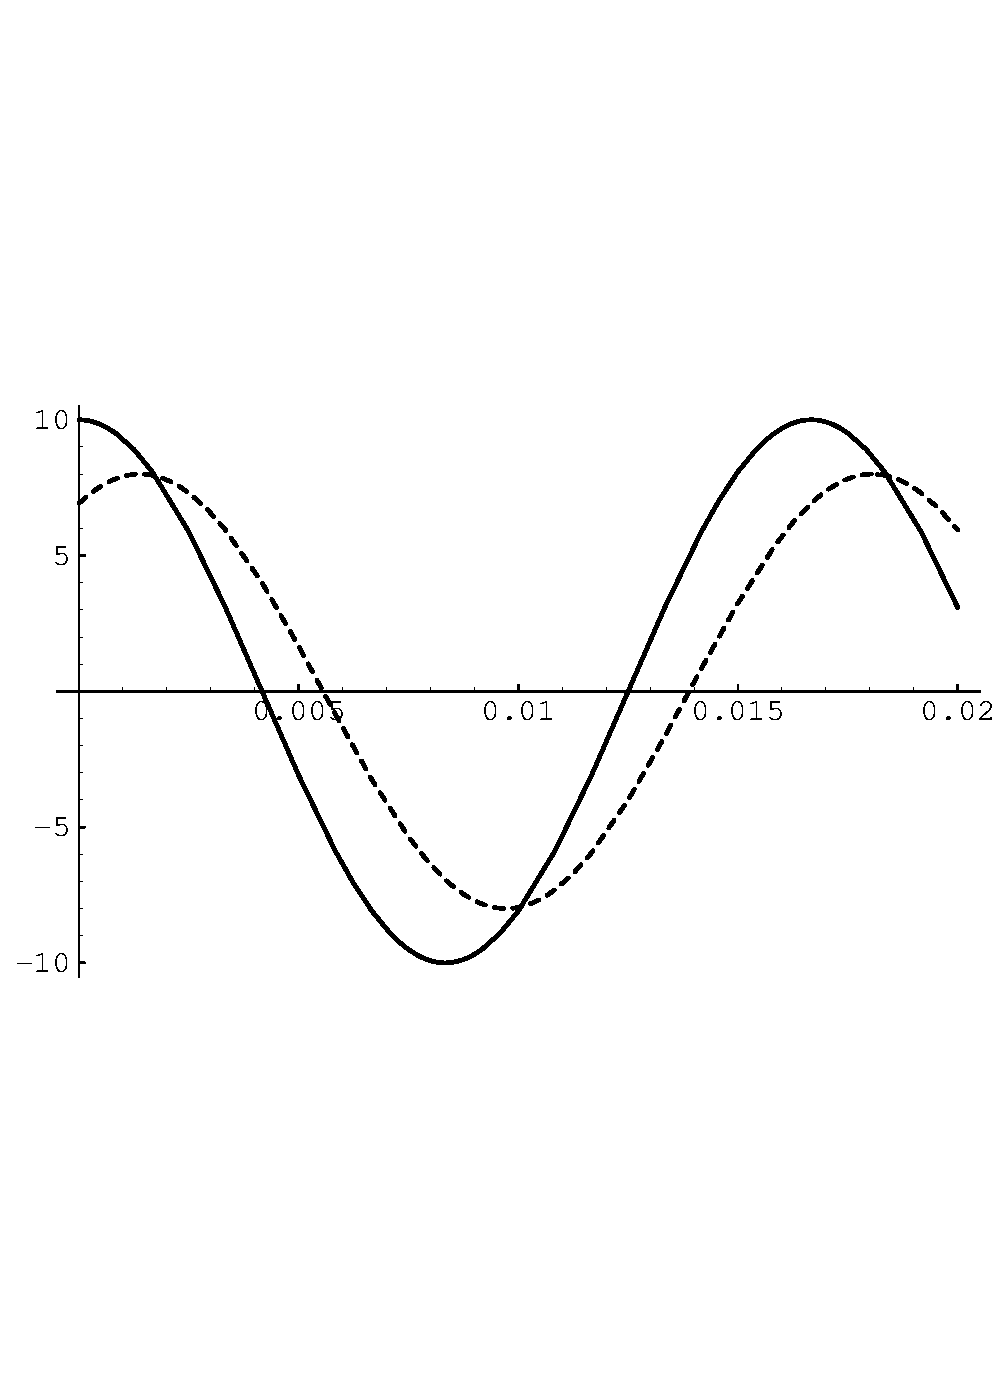
\epsfig{file=Figures/figure8.ps,height=5cm,bbllx=60pt,bblly=250pt,
bburx=550pt,bbury=530pt}
\caption{ \label{f:phase} This shows a driving voltage $V_{\rm coil}$
(solid curve) and the response voltage $V_{\rm IFO}$ (dotted curve) as
functions of time (in sec).  Both are 60 Hz sinusoids; the relative
amplitude and phase of the in-phase and out-of-phase components of
$V_{\rm IFO}$ are contained in the swept-sine calibration files.}
\end{center}
\end{figure}

We will shortly address the following question.  How does one use the
dimensionless data in the {\tt channel.0} files to reconstruct the
differential motion $\Delta l(t)$ (in meters) of the interferometer
arms?  Here we address the closely related question:  given $V_{\rm
IFO}$, how do we reconstruct $V_{\rm coil}$?  We choose the sign
convention for the Fourier transform which agrees with that of {\it
Numerical Recipes}:  equation (12.1.6) of \cite{NumRec}.  The Fourier
transform of a function of time $V(t)$ is
\begin{equation}
\label{e:fft1}
{\tilde V}(f) = \int {\rm e}^{2 \pi i f t} V(t) dt.
\end{equation}
The inverse Fourier transform is
\begin{equation}
\label{e:fft2}
V(t)= \int {\rm e}^{-2 \pi i f t} {\tilde V}(f) df.
\end{equation}
With these conventions, the signals (\ref{e:calibrate1}) and
(\ref{e:calibrate2}) shown in in Figure~\ref{f:phase} have Fourier
components:
\begin{eqnarray}
{\tilde V}_{\rm coil}(60) = 5                  \quad &{\rm and}& \quad {\tilde V}_{\rm coil}(-60) = 5,\\
{\tilde V}_{\rm IFO}(60)  = 4{\rm e}^{i \pi/6} \quad &{\rm and}& \quad {\tilde V}_{\rm IFO}(-60)  = 4 {\rm e}^{-i \pi/6}.
\end{eqnarray}
At frequency $f_0=60$ Hz the swept sine file
contains
\begin{equation}
S(60) = 0.8 \; {\rm e}^{-i \pi/6} \Rightarrow S(-60) = S^*(60) =
0.8 \; {\rm e}^{i \pi/6}.
\end{equation}
since $S(-f) = S^*(f)$.

With these choices for our conventions, one can see immediately from our
example (and generalize to all frequencies) that
\begin{equation}
\label{e:coilcon}
{\tilde V}_{\rm coil}(f) = {{\tilde V}_{\rm IFO} \over S^*(f)}.
\end{equation}
In other words, with the {\it Numerical Recipes} \cite{NumRec}
conventions for forward and reverse Fourier Transforms, the (FFT of
the) calibration-coil voltage is  the (FFT of the) IFO-output
voltage divided by the complex conjugate of the swept sine response.
\begin{description}
\item{Author:}  Bruce Allen, ballen@dirac.phys.uwm.edu
\item{Comments:}  The swept-sine calibration curves are usually quite
smooth but sometimes they contain a ``glitch" in the vicinity of
1 kHz; this may be due to drift of the unity-gain servo point.
\end{description}
\clearpage

\subsection{Function: {\tt calibrate()}}
\setcounter{equation}0
{\tt void calibrate(FILE *fpss,int num,float *complex,float srate,int
method,int order) }\\
This is a intermediate-level routine which reads in a 3-column ASCII
file of swept sine calibration data used to calibrate the IFO, and
outputs an array of interpolated points suitable for calibration of
FFT's of the interferometer output.

The arguments are:
\begin{description}
\item{\tt fpss:} Input.  Pointer to the file in which the
  swept sine data can be found.  The format of this data is described
  below.
\item{\tt srate:} Input.  The sample rate $F_{\rm sample}$ (in Hz) of the data that
  we are going to be calibrating.
\item{\tt num:} Input.  The number of points $N$ in the FFT that we
 will be calibrating.  This is typically $N=2^k$ where $k$ is an
 integer.  In this case, the number of distinct frequency values at
 which a calibration is needed is $2^{k-1}+1 = N/2+1$, corresponding to
 the number of distinct frequency values from $0$ (DC) to the Nyquist
 frequency $f_{\rm Nyquist}$.  See for example equation (12.1.5) of
 reference \cite{NumRec}.  The frequencies are $f_i = {i \over N}
 F_{\rm sample}$ for $i=0,\cdots,N/2$.
\item{\tt complex:} Input.  Pointer to an array {\tt complex[0..s]}
  where $s=2^k+1$.  The routine {\tt  calibrate()} fills in this array
  with interpolated values of the swept sine calibration data,
  described in the previous section.  The real part of the DC response
  is in {\tt complex[0]}, and the imaginary part is in {\tt
  complex[1]}. The real/imaginary parts of the response at frequency
  $f_1$ are in {\tt complex[2]} and {\tt complex[3]} and so on.  The
  last two elements of {\tt complex[ ]} contain the real/imaginary parts
  of the response at the Nyquist frequency $F_{\rm sample}/2$.
\item{\tt method:} Input.  This integer sets the type of interpolation
  used to determine the real and imaginary part of the response, at
  frequencies that lie in between those given in the swept sine
  calibration files.  Rational function interpolation is used if {\tt
  method}=0.  Polynomial interpolation is used if {\tt method}=1.
  Spline interpolation with natural boundary conditions (vanishing
  second derivatives at DC and the Nyquist frequency) is used if {\tt
  method}=2.
\item{\tt order:}  Input.  Ignored if spline interpolation is used.
  If polynomial interpolation is used, then {\tt order} is the order
  of the interpolating polynomial.
  If rational function interpolation is used, then the numerator and
  denominator are both polynomials of order {\tt order}/2 if {\tt order}
  is even; otherwise the degree of the denominator is ({\tt order}+1)/2
  and that of the numerator is ({\tt order}-1)/2.
\end{description}

The basic problem solved by this routine is that the swept sine
calibration files typically contain data at a few hundred distinct
frequency values.   However to properly calibrate the IFO output, one
usually needs this calibration information at a large number of
frequencies corresponding to the distinct frequencies associated with
the FFT of a data set.  This routine allows you to choose different
possible interpolation methods.  If in doubt, we recommend spline
interpolation as the first choice.  The interpolation methods are
described in detail in Chapter 3 of reference \cite{NumRec}.
\begin{description}
\item{Author:}  Bruce Allen, ballen@dirac.phys.uwm.edu
\item{Comments:}  It might be better to interpolate values of
$f^2$ times the swept-sine response function, as this is the quantity
needed to compute the IFO response function.
\end{description}
\clearpage

\subsection{Example: {\tt print\_ss} program}
\setcounter{equation}0
This example uses the function {\tt calibrate()} to read in a swept
sine calibration file, and then prints out a list of frequencies, real,
and imaginary parts interpolated from this data.  The frequencies are
appropriate for the FFT of a 4096 point data set with sample rate {\tt
srate}.   The technique used is spline interpolation.
\lgrindfile{Includes/print_ss.tex}

\clearpage
\subsection{Function: {\tt normalize\_gw()}}
\label{s:normalize}
\setcounter{equation}0
{\tt void normalize\_gw(FILE *fpss,int npoint,float srate,float *response)}

This routine generates an array of complex numbers $R(f)$ from the
information in the swept sine file and an overall calibration
constant.  Multiplying this array of complex numbers by (the FFT of)
{\tt channel.0} yields the (FFT of the) differential displacement of
the interferometer arms $\Delta l$, in meters: $\widetilde{\Delta l}(f)
= R(f) \widetilde{C_0}(f)$.  The units of $R(f)$ are meters/ADC-count.

The arguments are:
\begin{description}
\item{\tt fpss:} Input.  Pointer to the file in which the swept sine normalization
  data can be found.
\item{\tt npoint:} Input.  The number of points $N$ of {\tt channel.0} which will be used
to calculate an FFT for normalization.
Must be an integer power of 2.
\item{\tt srate:}  Input.  The sample rate in Hz of {\tt channel.0}.
\item{\tt response:} Output.  Pointer to an array {\tt response[0..s]}
with $s=N+1$ in which $R(f)$ will be returned.   By convention,
$R(0)=0$ so that {\tt response[0]=response[1]=0}.    Array elements
{\tt response[$2 i$]} and {\tt response[$2 i + 1$]} contain the real and
imaginary parts of $R(f)$ at frequency $f= i{\tt srate}/N$.   The
response at the Nyquist frequency {\tt response[N]=0} and {\tt
response[N+1]=0} by convention.
\end{description}

The absolute normalization of the interferometer can be obtained from
the information in the swept sine file, and one other normalization
constant which we denote by $Q$.  It is easy to understand how this
works.  In the calibration process, one of the interferometer end
mirrors of mass $m$ is driven by a magnetic coil.  The equation of
motion of the driven end mass is
\begin{equation}
m {d^2 \over dt^2} {\Delta l} = F(t)
\end{equation}
where $F(t)$ is the driving force and $\Delta l$ is the differential
length of the two interferometer arms, in meters.  Since the driving
force $F(t)$ is proportional to the coil current and thus to the coil
voltage, in frequency space this equation becomes
\begin{equation}
(- 2 \pi i f)^2 \widetilde{\Delta l}  = {\rm constant} \times \widetilde{V}_{\rm coil} =
{\rm constant} \times {{\tilde V}_{\rm IFO} \over S^*(f)}.
\end{equation}
We have substituted in equation (\ref{e:coilcon}) which relates
${\tilde V}_{\rm IFO}$ and ${\tilde V}_{\rm coil}$.
The IFO voltage is directly proportional to the quantity recorded in 
{\tt channel.0}: $V_{\rm IFO} = {\rm ADC} \times C_0$, with the constant ${\rm ADC}$ 
being the ratio of the analog-to-digital converter's input voltage to
output count.

Putting together these factors, the
properly normalized value of $\Delta l$, in meters, may be obtained
from the information in {\tt channel.0}, the swept sine file, and the
quantities given in Table~\ref{t:units} by
\begin{equation}
\label{e:rdef}
\widetilde{\Delta  l} = R(f) \times \widetilde{C_0 }  \qquad {\rm with } \quad
R(f) = {Q  \times {\rm ADC}  \over -4 \pi^2 f^2 S^*(f)},
\end{equation}
where the $\tilde {}$ denotes Fourier transform, and $f$ denotes
frequency in Hz.  (Note that, apart from the complex conjugate on $S$,
the conventions used in the Fourier transform drop out of this
equation, provided that identical conventions
(\ref{e:fft1},\ref{e:fft2}) are applied to both $\Delta l$ and to
$C_0$).
\begin{table}[h]
\caption{Quantities entering into normalization of the IFO output.}
\label{t:units}
\begin{center}
\begin{tabular}[]{c|c|c|c}
Description            & Name      &  Value                & Units \\
\hline
Gravity-wave signal ({\tt channel.0})   & $C_0$  &  varies               & ADC counts \\
\hline
A$\rightarrow$D converter sensitivity & ADC       &  10/2048              &    $ \rm V_{\rm IFO} \left({\rm ADC\ counts}\right)^{-1}      $ \\
\hline
Swept sine calibration & S(f)        &  from file            &  $   \rm V_{\rm IFO}  \left( V_{\rm coil}\right) ^{-1} $ \\
\hline
Calibration constant   &  $Q$      & $1.428\times 10^{-4}$ &  $ \rm meter\ Hz^2 \left(  V_{\rm coil} \right)^{-1} $
\end{tabular}
\end{center}
\end{table}
The constant quantity $Q$ indicated in the above equations has been
calculated and documented in a series of calibration experiments
carried out by Robert Spero. In these calibration experiments, the
interferometer's servo was left open-loop, and the end mass was driven at
a single frequency, hard enough to move the end mass one-half wavelength
and shift the interference fringe's pattern over by one fringe.  In this
way, the coil voltage required to bring about a given length motion at
a particular frequency was established, and from this information, the
value of $Q$ may be inferred.  During the November 1994 runs the value
of $Q$ was given by
\begin{equation}
Q = {\sqrt{9.35 \; \rm Hz} \over k} = 1.428 \times 10^{-4} {\rm
meter\ Hz^2 \over V_{\rm coil}} \qquad {\rm where\ } k=21399 {\rm
\ V_{\rm coil} \over meter \; Hz^{3/2}}.
\end{equation}

\begin{description}
\item{Author:}  Bruce Allen, ballen@dirac.phys.uwm.edu
\item{Comments:}  See comment for {\tt calibrate()}.
\end{description}
\clearpage

\subsection{Example: {\tt power\_spectrum} program}
\setcounter{equation}0
This example uses the function {\tt normalize\_gw()} to produce a
normalized, properly calibrated power spectrum of the interferometer
noise, using the gravity-wave signal from {\tt channel.0}, the TTL-lock
signal from {\tt channel.10} and a swept-sine calibration curve.

The output of this program is a 2-column file; the first column is
frequency and the second column is the noise in units of $\rm
meters/\sqrt{\rm Hz}$.

A couple of comments are in order here:
\begin{description}
\item{1.} 
Even though we only need the modulus, for pedagogic reasons, we explicitly
calculate both the real and imaginary parts of $\widetilde{\Delta l}(f)=
R(f) \widetilde{C_0}(f)$.
\item{2.}
The fast Fourier transform of $\Delta l$, which we denote ${\rm
FFT}[\Delta l]$, has the same units (meters!) as $\Delta l$.  As can be
immediately seen from {\it Numerical Recipes} equation (12.1.6) the
Fourier transform $\widetilde{\Delta l}$ has units of meters-sec and is
given by $\widetilde{\Delta l} =\Delta t \; {\rm FFT}[\Delta l]$, where
$\Delta t$ is the sample interval.  The (one-sided) power spectrum of
$\Delta l$ in $\rm meters/\sqrt{\rm Hz}$ is $P=\sqrt{2 \over T}
| \widetilde{\Delta l} | $ where $T=N \Delta t$ is the total length of the
observation interval, in seconds.  Hence one has
\begin{equation}
P=\sqrt{2 \over N \Delta t} \; \Delta t \; | {\rm FFT}[\Delta l] |=
\sqrt{2 \Delta t \over N} \; | {\rm FFT}[\Delta l] |.
\end{equation}
This is the reason for the factor which appears in
this example.
\item{3.} To get a spectrum with decent frequency resolution, the time-domain
data must be windowed (see the example program {\tt calibrate} and the function
{\tt avg\_spec()} to see how this works).
\end{description}
A sample of the output from this program is shown in Figure~\ref{f:pspec}.

\begin{figure}[hb]
\begin{center}
\index{colorpage}
\epsfig{file=Figures/figure9.ps,height=7.5cm,bbllx=25pt,bblly=85pt,
bburx=525pt,bbury=510pt}
\caption{\label{f:pspec} An example of a power spectrum curve produced
with {\tt power\_spectrum}.  The spectrum produced off a data tape
(with 100 point smoothing) is compared to that produced by the HP
spectrum analyzer in the lab.}
\end{center}
\end{figure}
\lgrindfile{Includes/power_spectrum.tex}

\begin{description}
\item{Author:}
Bruce Allen, ballen@dirac.phys.uwm.edu
\item{Comments:}
The IFO output typically consists of a number of strong line sources
(harmonics of the 60 Hz line and the 180 Hz laser power supply, violin
modes of the suspension, etc) superposed on a continuum background
(electronics noise, laser shot noise, etc)  In such situations, there
are better ways of finding the noise power spectrum (for example, see the
multi-taper methods of David J. Thompson \cite{thomson82}, or the textbook
by Percival and Walden \cite{percivalwalden}). Using methods such as the
F-test to remove line features from the time-domain data stream might
reduce the sidelobe contamination (bias) from nearby frequency bins,
and thus permit an effective reduction of instrument noise near these
spectral line features.  Further details of these methods, and some
routines that implemen them, may be found in Section~\ref{ss:mtapintro}.
\end{description}
\clearpage

\subsection{Example: {\tt calibrate} program}
\setcounter{equation}0
This example uses the function {\tt normalize\_gw()} and {\tt
avg\_spec()} to produce an animated display, showing the properly
normalized power spectrum of the interferometer, with a 30-second
characteristic time moving average.  After compilation, to run the
program type:\\
\indent {\tt calibrate $|$ xmgr -pipe \&} \\
to get an animated display showing the calibrated power spectrum
changing.  An example of the output from {\tt calibrate} is shown in
Figure~\ref{f:calibrate}.  Note that most of the execution time here is
spent passing data down the pipe to {\tt xmgr} and displaying it.  The
display can be speeded up by a factor of ten by binning the
output values to reduce their number to a few hundred lines (the example
program {\tt calibrate\_binned.c} implements this technique; it can be
run by typing {\tt calibrate\_binned | xmgr -pipe}).

\begin{figure}[hb]
\index{colorpage}
\begin{center}
\epsfig{file=Figures/figure11.ps,height=7cm,bbllx=30pt,bblly=85pt,
bburx=525pt,bbury=510pt}
\caption{\label{f:calibrate} 
This shows a snapshot of the output from the program {\tt calibrate}
which displays an animated average power spectrum (Welch windowed, 30-second decay time).}
\end{center}
\end{figure}

\lgrindfile{Includes/calibrate.tex}

\begin{description}
\item{Author:}
Bruce Allen, ballen@dirac.phys.uwm.edu
\item{Comments:}
See comments for {\tt power\_spectrum} example program.
\end{description}
\clearpage

\subsection{Example: {\tt transfer} program}
\label{ss:impulse-response}
\setcounter{equation}0
This example uses the function {\tt normalize\_gw()} to calculate the
response of the interferometer to a specified gravitational-wave strain
$h(t)$. [Note: for clarity, in this example, we have NOT worried about
getting the overall normalization correct.] The code includes two
possible $h(t)$'s.  The first of these is a binary-inspiral chirp (see
Section~\ref{s:inspiral}).  Or, if you un-comment one line of code, you
can see the response of the detector to a unit-impulse gravitational
wave strain, in other words, the impulse response of the detector.

Note that to run this program, you must specify
a path to the 40-meter data, for example by typing:\\
\indent {\tt setenv GRASP\_DATAPATH /usr/local/data/19nov94.3}\\ 
so that the code can find a swept-sine calibration file to use.

The response of the detector to a pair of inspiraling stars is shown in
Figure~\ref{f:detresp}.  You will notice that although the chirp starts at
a (gravitational-wave) frequency of 140 Hz on the left-hand side of the
figure, the low-frequency response of the detector is so poor that the
chirp does not really become visible until about half-a-second later,
at somewhat higher frequency.  In the language of the audiophile, the
IFO has crummy bass response!  Of course this is entirely deliberate;
the whitening filters of the instrument are designed to attenuate the
low-frequency seismic contamination, and consequently also attenuate
any possible low-frequency gravitational waves.

\begin{figure}[hb]
\begin{center}
\epsfig{file=Figures/transfer.ps,angle=-90,width=5in}
\caption{\label{f:detresp}
Output produced by the {\tt transfer} example program.
The top graph shows the gravitational-wave strain produced by an
inspiraling binary pair.  The lower graph shows the calculated
interferometer output [channel.0  or IFO\_DMRO] produced by this
signal.  Notice that because of the poor low-frequency response of the
instrument, the IFO output does not show significant response before
the input frequency has increased.  The sample rate is slightly under
10 kHz.
}
\end{center}
\end{figure}

The response of the detector to a unit gravitational strain impulse is
shown as a function of time-offset in Figure~\ref{f:detresp2}.  Here
the predominant effect is the ringing of the anti-aliasing filter.  The
impulse response of the detector lasts about 30 samples, or 3 msec.
For negative offset times the impulse response is quite close to zero;
its failure to vanish is partly a wrap-around effect, and partly due to
errors in the actual measurement of the transfer function.

\begin{figure}[hb]
\begin{center}
\epsfig{file=Figures/impulse.ps,angle=-90,width=4in}
\caption{\label{f:detresp2}
Output produced by the {\tt transfer} example program.
This shows the calculated
interferometer output [channel.0  or IFO\_DMRO] produced by
an impulse in the gravitational-wave strain at sample number zero.
This (almost) causal impulse response lasts about 3 msec.
}
\end{center}
\end{figure}

This is a good place to insert a cautionary note.  Now that we have
determined the transfer function $R(f)$ of the instrument, you might be
tempted to ask: ``Why should I do any of my analysis in terms of the
instrument output?  After all, my real interest is in gravitational
waves.  So the first thing that I will do in my analysis is convert the
instrument output into a gravitational wave strain $h(t)$ at the
detector, by convolving the instrument's output with (the time-domain
version of) $R(f)$."  {\bf Please do not make this mistake!} A few moment's
reflection will show why this is a remarkably bad idea.  The problem
is that the response function $R(f)$ is extremely
large at low frequencies.  This is just a reflection of the poor low
frequency response of the instrument: any low-frequency energy in the
IFO output corresponds to an extremely large amplitude low frequency
gravitational wave.  So, if you calculate $h(t)$ in the way described:
take a stretch of (perhaps zero-padded) data, FFT it into the frequency domain,
multiply it by $R(f)$ and invert the FFT to take it back into the frequency
domain, you will discover the following:
\begin{itemize}
\item
Your $h(t)$ is dominated by a single low-frequency noisy sinusoid
(whose frequency is determined by the low frequency cutoff imposed by
the length of your data segment or the low-frequency cutoff of the
response function).
\item
Your $h(t)$ has {\it lost} all the interesting information present at
frequencies where the detector is quiet (say, around 600 Hz).  Because
the noise power spectrum (see Figure~\ref{f:pspec}) covers such a large
dynamic range, you can not even represent $h(t)$ in a floating point
variable (though it will fit, though barely, into a double).  This is
why the instrument uses a whitening filter in the first place.
\item
It is possible to construct ``$h(t)$" if you filter out the
low-frequency garbage by setting $R(f)$ to zero below (say) 100 Hz.
\end{itemize}
If you are unconvinced by this, do the following exercise:  calculate
the power spectrum in the frequency domain as was done with
Figure~\ref{f:pspec}, then construct $h(t)$ in time time domain, then
take $h(t)$ back into the frequency domain, and graph the power
spectrum again.  You will discover that it has completely changed above
100 Hz and is entirely domainted by numerical quantization noise
(round-off errors).

\lgrindfile{Includes/transfer.tex}

\begin{description}
\item{Author:}
Bruce Allen, ballen@dirac.phys.uwm.edu
\item{Comments:}
None.
\end{description}
\clearpage

\subsection{Example: {\tt diag} program}
\setcounter{equation}0
This program is a frequency-domain ``novelty detector" and provides a
simple example of a time-frequency diagnostic method.  
The actual code is not printed here, but may be found in the GRASP directory
{\tt src/examples/examples\_40meter} in the file {\tt diag.c}.

The method used by {\tt diag} is as follows:
\begin{enumerate}
\item
A buffer is loaded with a short stretch of data samples (2048 in this
example, about 1/5 of a second).
\item
A (Welch-windowed) power spectrum is calculated from the data in 
the buffer.  In each frequency bin,
 this provides a value $S(f)$.
\item
Using the same auto-regressive averaging technique described in {\tt
avg\_spec()} the mean value of $S(f)$ is maintained in a time-averaged
spectrum $\langle S(f) \rangle$.  The exponential-decay time constant
for this average is {\tt AVG\_TIME} (10 seconds, in this example).
\item
The absolute difference between the current spectrum and the average
$\Delta S(f) \equiv |S(f) - \langle S(f) \rangle |$ is determined. Note
that the absolute value used here provides a more robust first-order
statistic than would be provided by a standard variance $(\Delta
S(f))^2$.
\item
Using the same auto-regressive averaging technique described in {\tt
avg\_spec()} the value of $\Delta S(f)$ is maintained in a
time-averaged absolute difference $\langle \Delta S(f) \rangle$.  The
exponential-decay time constant for this average is also set by {\tt
AVG\_TIME}.
\item
In each frequency bin, $\Delta S(f)$ is compared to $\langle \Delta
S(f) \rangle$.  If $\Delta S(f) > {\tt THRESHOLD} \times \langle \Delta
S(f) \rangle$ then a point is plotted for that frequency bin; otherwise
no point is plotted for that frequency bin.  In this example, {\tt
THRESHOLD} is set to 6.
\item
In each frequency bin, $\Delta S(f)$ is compared to $\langle \Delta
S(f) \rangle$.  If $\Delta S(f) < {\tt INCLUDE} \times \langle \Delta
S(f) \rangle$ then the values of $S(f)$ and $\Delta S(f)$ are used to
``refine" or ``revise" the auto-regressive means described previously.
In this example, {\tt INCLUDE} is set to 10.
\item
Another set of points (1024 in this example) is loaded into the
end of the buffer, pushing out the oldest 1024 points from the start
of the buffer, and the whole loop is restarted at step 2 above.
\end{enumerate}
The {\tt diag} program can be used to analyze any of the different
channels of fast-sampled data, by setting {\tt CHANNEL}
appropriately.  It creates one output file for each locked segment of
data.  For example if {\tt CHANNEL} is set to 0 (the IFO channel)
and there are four locked sections of data, one obtains a set of
files:\\
{\tt ch0diag.000}, 
{\tt ch0diag.001}, 
{\tt ch0diag.002}, and
{\tt ch0diag.003}.\\
In similar fashion, if {\tt CHANNEL} is set to 1 (the magnetometer)
one obtains files:\\
{\tt ch1diag.000}, 
{\tt ch1diag.001}, 
{\tt ch1diag.002}, and
{\tt ch1diag.003}.\\
These files may be used as input to the {\tt xmgr} graphing program,
by typing:\\
{\tt xmgr ch0diag.000 ch1diag.000}\\
(one may specify as many channels as desired on the input line).  A
typical pair of outputs is shown in Figures~\ref{f:diag0} and
\ref{f:diag1}.  By specifying several different channels on the command
line for starting {\tt xmgr}, you can overlay the different channels
output with one another.  This provides a visual tool for identifying
correlations between the channels (the graphs shown below may be
overlaid in different colors).
\begin{description}
\item{Author:}
Bruce Allen, ballen@dirac.phys.uwm.edu
\item{Comments:}
This type of time-frequency event detector appears quite useful as a
diagnostic tool.  It might be possible to improve its high-frequency
time resolution by being clever about using intermediate information
during the recursive calculation of the FFT.  One should probably also
experiment with using other statistical measures to assess the behavior
of the different frequency bins.  It would be nice to modify this
program to also examine the slow sampled channels (see comment for {\tt
get\_data()}).
\end{description}
\begin{figure}[t]
\begin{center}
\epsfig{file=Figures/figure13a.ps,angle=270,width=5in}
\caption{ \label{f:diag0} A time-frequency diagnostic graph produced by
{\tt diag}.  The vertical line pointed to by the arrow is a
non-stationary noise event in the IFO output, 325 seconds into the
locked section.  It sounds like a ``drip" and might be due to off-axis
modes in the interferometer optical cavities.}
\end{center}
\end{figure}
\begin{figure}[b]
\index{colorpage}
\begin{center}
\epsfig{file=Figures/figure13b.ps,angle=270,width=5in}
\caption{ \label{f:diag1} A time-frequency diagnostic graph
produced by {\tt diag}.  This shows the identical period as the previous
graph, but for the magnetometer output.  Notice that the spurious event
was not caused by magnetic field fluctuations.}
\end{center}
\end{figure}
\label{s:endof40m}
\clearpage

% /* GRASP: Copyright 1997,1998  Bruce Allen */
% $Id: man_frame.tex,v 1.37 1999/07/11 21:22:10 ballen Exp $
\section{GRASP Routines: Reading/using FRAME format data}
\setcounter{equation}0
\label{s:frameformat}
The LIGO and VIRGO projects have recently adopted a data format standard
called the FRAME format for time-domain data.  The 40-meter laboratory
at Caltech implemented this data format in Spring 1997; data taken after
that time is in the FRAME format.  The FRAME libraries are publicly
available from the VIRGO project; they may be downloaded from the site
\htmladdnormallink{{\tt http://wwwlapp.in2p3.fr/virgo/FrameL}.}
{http://wwwlapp.in2p3.fr/virgo/FrameL}
The GRASP package has been
tested up to release 3.72 of the frame library. Contact Benoit Mours\linebreak[4]
{\tt mours@lapp.in2p3.fr} for further information.

The GRASP package includes routines for reading and using data in the
FRAME format.  Also included in the GRASP package is a translator (see
Section~\ref{ss:translate}) which translates data from the old data format
used in 1994 to the new FRAME format.  Data distributed for use with
GRASP will primarily be distributed in this new FRAME format, and over
a period of time we will remove from the GRASP package all of the code
and routines which make use of the old format.  In order to help make
the transition from old format to FRAME format as smooth as possible,
the GRASP package currently contains both old format and FRAME format
versions of all of the example programs.  For example {\tt animate}
and {\tt animateF} are two versions of the same program.  The first
reads data in the old format, the second reads data in the FRAME format.
If you are new to GRASP, we don't recomend that you waste your time with
the old data format; start using the FRAME format immediately.

Data distributed in the FRAME format may not be compatible with future
releases of the FRAME library, so if the FRAME libraries are updated you
may need to obtain a new copy of the standard 40-meter test data set from
November 1994.  The data that has been distributed and is currently being
distributed makes use of either version 2.20, 2.30 or 2.37 of the
FRAME library.  We will shortly begin distributing data in version
3.50 of the FRAME format.
Only two files in the GRASP package ({\tt src/\-utility/\-frameinterface.c}
and {\tt src/\-examples/\-examples\_utility/\-translate.c}) depend upon the
version of the FRAME library.  We distribute GRASP with versions of
these files appropriate for different releases.
The files determine the version of the frame library at compilation
time, and then include the appropriate code.  This code works
correctly with any version of the frame library $2.37 \le {\rm
version} \le 3.70$.  Note that version $\ge 3.50$ of the frame library can
read data written by any version back to and including 2.37.

One of the nice properties of the FRAME formats $\ge 3.30$ is that
they support a ``compressed" format.  This is transparent to the user
(except that reading the ``compressed" frames takes a bit longer because the
frame library then needs to uncompress the data).  Data distributed in version
3.50 of the FRAME format is being distributed in this compressed form and
occupies somewhat less space than the old-format original data. As shown
in Section~\ref{s:40meter} the old-format data for the November 1994 runs
occupied about 13.6 Gbytes. For comparison, the FRAME-format data
occupies less than half of that space:
{\tt
\begin{verbatim}
     14nov94.1.frame 314
     14nov94.2.frame 397
     18nov94.1.frame 503
     18nov94.2.frame 543
     19nov94.1.frame 551   The space occupied
     19nov94.2.frame 535   is shown in Mbytes
     19nov94.3.frame 641
     19nov94.4.frame 605
     20nov94.1.frame 553
     20nov94.2.frame 422
     20nov94.3.frame 755
\end{verbatim}
}
\noindent
The total storage space required for FRAME 3.50 data totals only 5.8 Gbytes.

In order to give the 1994 40-meter data a form as similar as possible
to the data being taken in 1997 and beyond, the channel names used
have been given equivalent ``FRAME" forms.  These are shown in
Table~\ref{t:chassignf}.

Note that new data created in the frame format attempts to address at
least a couple of the problems in the ``old format" data.  In particular,
new frame format data (i.e., post 1996) has sample rate in Hz always being
powers of 2, for example, 4,096 Hz or 16 Hz or 16,384 Hz.  In addition,
each frame always contains a power-of-two number of seconds of data.
These conventions will make it easy to ``match up" sample of channels
taken at different rates, and to do FFT's of the channels.  However the
1994 data does not conform to either of these conventions: each frame of
1994 data contains 5000 samples of the slow channels, and 50,000 samples
of the fast channels, during a $5.06666\cdots$ second interval.

\begin{table}[h]
\begin{tabular}[]{c|c|c|c|c}
\hline
Channel \# & $\le$ 14 Nov 94 & FRAME name &  $\ge$ 18 Nov 94 & FRAME name\\
\hline
0 & IFO output & IFO\_DMRO & IFO output & IFO\_DMRO\\
1 & unused & & magnetometer & IFO\_Mag\_x \\
2 & unused &  & microphone & IFO\_Mike\\
3 & microphone & IFO\_Mike& unused & \\
\hline
4 & dc strain & IFO\_DCDM & dc strain & IFO\_DCDM \\
5 & mode cleaner pzt & PSL\_MC\_V & mode cleaner pzt & PSL\_MC\_V \\
6 & seismometer & IFO\_Seis\_1 & seismometer & IFO\_Seis\_1 \\
7 & unused & & slow pzt & IFO\_SPZT \\
8 & unused& & power stabilizer  & PSL\_PSS \\
9 & unused  & & unused & \\
10 & TTL locked & IFO\_Lock &  TTL locked & IFO\_Lock \\
11 & arm 1 visibility& IFO\_EAT & arm 1 visibility & IFO\_EAT\\
12 & arm 2 visibility & IFO\_SAT &  arm 2 visibility &  IFO\_SAT\\
13 & mode cleaner visibility & IFO\_MCR & mode cleaner visibility & IFO\_MCR\\
14 & slow pzt & IFO\_SPZT &  unused & \\
15 & arm 1 coil driver & SUS\_EE\_Coil\_V & arm 1 coil driver & SUS\_EE\_Coil\_V \\
\hline
\end{tabular}
Note: {\small On 18 November 1994 run 1 the power stabilizer was
accidentally disconnected until approximately 20:00 local time.}
\caption{Channel assignments for the November 1994 data runs.  Channels
0-3 are the ``fast" channels, sampled at about 10 kHz; the remaining
twelve are the ``slow" channels, sampled at about 1KHz.  The equivalent
``FRAME" format names are also given.}
\label{t:chassignf}
\end{table}
\clearpage

\subsection{Time-stamps in the November 1994 data-set}
\label{ss:timestamp}
\setcounter{equation}0
There is a serious problem in the original data format used in November
1994.  To understand the nature of this problem, remember that the
individual data samples (fast channels) are taken at about 10kHz,
so that the time between samples is about 100 $\mu$sec.  Ideally, the
time-stamps of the individual blocks should be recorded with a precision which
is substantially greater than this, i.e. a few $\mu$sec at the most.
However the November 1994 time stamps are recorded in two ways:  as an
integer number of seconds and msec (with 1000 $\mu$sec resolution) and
as a floating point elapsed time.  This latter quantity has a resolution
of less than one $\mu$sec at early times, but a resolution of about 2000
$\mu$sec at late times (say 15,000 sec into a run).

Thus, in translating the November 1994 data into frames (which have
1 nanosec resolution time-stamps), a reasonable effort was made
to ``correct" these time-stamps as much as possible, and to specify
the time at which each data block begins as precisely as possible.
After some research, we believe that the each block of old-format data is
precisely $76/15=5.0666666 \cdots$ seconds long.  So we have corrected
the time stamps accordingly.  One can show that in general, our time
stamps agree with those in the original data, when they are expressed
as floats, i.e. with the precison recorded in the original data set.
There are some blocks where there is an error in the least-significant
bit of the cast-into-float quantity; we do not understand this as well
as we would like.

Please, {\it be warned that the absolute time indicated by these stamps
is not correct!} These time stamps were not taken with a modern GPS clock
system, or even with an old-fashioned WWV system.  Our understanding is
that the real-time computer system on which these data were originally
taken had its clock set by wristwatch, with an accuracy of perhaps
$\pm 5$ minutes..  Indeed the computer system crashed on November 15,
1994 and the clock was subsequently reset again, so even the time
difference can not be trusted between November14 and November18 data.
It appears that the computer clock was not reset after November15th,
so the relative times in the remaining data may be trustworthy with
somewhat better than $\pm 1$ msec accuracy.

In any data anaysis work (such as pulsar searching) where it is
important to have precise time-stamps, these shortcomings must be taken
into account.  If you really want to determine the times more precisely
than a millisecond, our only suggestion is to examine the seismometer
data channel and correlate it with similar data taken by a system with
good time-stamps.  We don't know where to find such data, but it might
exist, somewhere, in the public domain.  If you do go to this trouble,
please write to us and tell us the conclusions of your study.  We would
be delighted to correct the absolute offset error in these November 1994
time-stamps, if someone could show us how to do it!
\clearpage

\subsection{Function: {\tt fget\_ch()} }
\setcounter{equation}0
{\tt int fget\_ch(struct fgetoutput *fgetoutput,struct fgetinput *fgetinput) }\\
\noindent
This is a general function for sequentially reading one or more
channels of FRAME format data.  It can be used to obtain either locked
sections only, or both locked and unlocked sections, and to retrieve
calibration information from the FRAME data.  It concatenates multiple
frames and multiple files containing frames as necessary, to return
continuous-in-time sequences.

The inputs to the routine {\tt fget\_ch()} are contained in a structure:
{\tt
\begin{verbatim}
struct fgetinput {
           int nchan;
           char **chnames;
           int npoint;
           short **locations;
           char *(*files)();
           int (*filedes)();
           int inlock;
           int seek;
           int calibrate;
           char *datatype; 
};
\end{verbatim}
}
The different elements of the structure are:
\begin{description}
\item{\tt nchan}: Input.  The number of channels that you want to retrieve ($ \ge 1$).
\item{\tt chnames}: Input.  The list of channel names.  Each element of
{\tt chnames[0..nchan-1]} is
   a pointer to a null-terminated string.  Note that the number of
   channels requested, and their names, must not be changed after the
   first call to {\tt fget\_ch}.  It is assumed that the first channel in
   the list has the fastest sample rate of any of the requested channels.
   As long as this assumption is satisfied, the channels may be accessed
   in any order.
\item{\tt npoint}: Input.  The number of points requested from the first channel.  (May change with each call.)
\item{\tt locations}: Input.  The locations in memory where the arrays corresponding to each channel should be placed
   are {\tt locations[0..nchan-1]}.   (May change with each call.)
\item{\tt files()}: Input.  A pointer to a function, which takes no
   arguments, and returns a pointer to a null-terminated character string.
   This string is the name of the file to look in for FRAME format data.
   If no further frames remain in the file, then the function {\tt
   files()} is called again.  When this function returns a null pointer,
   it is assumed that no further data remains.  A useful utility function
   called {\tt framefiles()} has been provided with GRASP, and may be
   used as this argument.  (May change with each call.)
\item{\tt filedes()}: Input.  This argument is used if and only if the
   previous argument, {\tt fgetinput.files} is {\tt NULL}.  If {\tt
   fgetinput.files} is not {\tt NULL} then this argument is not used.
   This argument is a pointer to a function, which takes no arguments,
   and returns an integer {\it file descriptor}.  The integer returned
   is a file descriptor for a file containing FRAME format data.  If no
   further frames remain in the file, then the function {\tt filedes()} is
   called again.  When this function returns a negative file descriptor,
   it is assumed that no further data remains.  (May change with each
   call.)
\item{\tt inlock}: Input.  Set to zero, return all data; set to non-zero, return only the locked sections of data.  If set nonzero, then on output {\tt fgetoutput.locklow} and {\tt fgetoutput.lockhi} will be set.
\item{\tt seek}: Input.  Set to zero, return data.  Set to non-zero,
   seek past the data, performing all normal operations, but do
   not actually write any data into the arrays pointed to by {\tt
   locations[0..nchan-1]}.  (May change with each call.)  This is useful
   for skipping rapidly past uninteresting regions of data, for example,
   the first few minutes after coming into lock.
\item{\tt calibrate}: Input.  If set non-zero, return calibration information.  If set to zero, do not return
   calibration information. (May change with each call.)
\item{\tt datatype}: Output. A character string indicating the data
   type in each channel. The coding is: C~= {\tt char}, S~= {\tt
     short}, D~= {\tt double}, F~= {\tt float}, I~= {\tt int}, L~= {\tt
     long}, f~= {\tt complex float}, d~= {\tt complex double}, s~= {\tt
     string}, u~= {\tt unsigned short}, i~= {\tt unsigned int}, l~=
     {\tt unsigned long}, c~= {\tt unsigned char}.  
\end{description}
\noindent
Except as noted above, it is assumed that none of these input arguments
are changed after the first call to {\tt fget\_ch()}.  It is also
assumed that within any given frame, the numbers of points contained
in different channels are exact integer multiples or fractions of the
numbers of points contained in the other channels.

The outputs from the routine {\tt fget\_ch()} are contained in a structure:
{\tt
\begin{verbatim}
struct fgetoutput {
           double tstart;
           double tstart_gps;
           double srate;
           int *npoint;
           int *ratios;
           int discarded;
           double tfirst;
           double tfirst_gps;
           double dt;
           double lostlock;
           double lostlock_gps;
           double lastlock;
           double lastlock_gps;
           int returnval;
           int frinum;
           float *fri;
           int tcalibrate;
           int tcalibrate_gps;
           int locklow;
           int lockhi;
           char *filename;
           char *slow_names; 
};
\end{verbatim}
}
The different elements of the structure are:
\begin{description}
\item{\tt  tstart}: Output. Time stamp of the first point output in channel {\tt chnames[0]}.
   Note: please see the comments in Section~\ref{ss:timestamp}.
Units are Unix-C time in seconds  defined in Section~\ref{s:timestandards}.
\item{\tt  tstart\_gps}: Output. Same as previous quantity, but with GPS time in seconds.
\item{\tt  srate}: Output.  Sample rate (in Hz) of channel {\tt chnames[0]}.
\item{\tt  npoint}: Output. The number of points returned in channel {\tt chnames[i]} is {\tt npoint[i]}.  Note
   that {\tt npoint[0]} is precisely the number of points requested in the input structure {\tt  fgetinput.npoint}.
\item{\tt  ratios}: Output.  The sample rate of channel {\tt chnames[0]} divided by the sample rate of
  channel {\tt chnames[i]} is given in {\tt ratios[i]}.  Thus {\tt ratios[0]=1}.
\item{\tt  discarded}: The number of points discarded from channel {\tt chnames[0]}.  These points are discarded
  because there is a missing period of time between two consecutive frames, or because the instrument was not in
  lock for long enough to return the requested number of points (or for both reasons).
\item{\tt  tfirst}: Output.  The time stamp of the first point returned in the first call to {\tt fget\_ch()}.   
Units are Unix-C time in seconds  defined in Section~\ref{s:timestandards}.
\item{\tt  tfirst\_gps}: Output.  Same as previous quantity, but with GPS time in seconds.
\item{\tt  dt}: Output.  By definition, {\tt tstart-tfirst}, which is the elapsed time since the first time stamp.
\item{\tt  lostlock}: Output.  The time at which we last lost lock (if searching only for locked segments).
Units are Unix-C time in seconds  defined in Section~\ref{s:timestandards}.
\item{\tt  lostlock\_gps}: Output.  Same as previous quantity, but with GPS time in seconds.
\item{\tt  lastlock}: Output.  The time at which we last regained lock (if searching only for locked segments).
Units are Unix-C time in seconds  defined in Section~\ref{s:timestandards}.
\item{\tt  lastlock\_gps}: Output.  Same as previous quantity, but with GPS time in seconds.
\item{\tt  returnval}: Output.  The return value of  {\tt fget\_ch()}:
  0 if it is unable to satisfy the request, 1 if the request has been
  satisfied by beginning a new locked or continuous-in-time section, and 2
  if the data returned is part of an ongoing locked or continuous-in-time
  sequence.
\item{\tt  frinum}: Output.  Three times the number of frequency values for which we are returning static calibration
    information.  If this number is not divisible by three, something is wrong!
\item{\tt  fri}: Output.  A pointer to the array of calibration data.  This data is arranged
 with a frequency, then the real part, then the imaginary part of
 the response, followed by another frequency, then real part, then
 imaginary part, etc.  So {\tt fri[0]=}$f_0$, {\tt fri[1]=}$r_0$,
 {\tt fri[2]=}$i_0$, {\tt fri[3]=}$f_1$, {\tt fri[4]=}$r_1$,
 {\tt fri[5]=}$i_1$,... and the total length of the array is {\tt
 fri[0..frinum-1]}.
\item{\tt  tcalibrate}: Output.  The time at which the current calibration information became valid.
Units are Unix-C time in seconds  defined in Section~\ref{s:timestandards}.
\item{\tt  tcalibrate\_gps}: Output.  Same as previous quantity, but with GPS time in seconds.
\item{\tt locklow}.  Output.  The minimum value (inclusive) for "in-lock" in the lock channel.
Set if and only if {\tt fgetinput.inlock} is nonzero.
\item{\tt lockhi}.  Output.  The maximum value (inclusive) for "in-lock" in the lock channel.
Set if and only if {\tt fgetinput.inlock} is nonzero.
\item{\tt filename}.  Output.  Points to a static character string containing
the name of the frame file currently in use, or {\tt NULL} is there is no
frame file open.
\item{\tt slow\_names}. Output. Names of the slow channels packed into one fast channel ``SLOW''.
\end{description}

Note that the time-stamps available in two different formats: Unix-C time in seconds 
and GPS time in seconds.  The relationship between these is described in detail in
Section~\ref{s:timestandards}.  In general, in new code the GPS time
stamps should be used, and taken as the more fundamental quantity.
The Unix-C time is the number of seconds after 00:00:00 Jan 1, 1970 UTC.
This is also known as
``Calendar Time" on Unix systems.  It is the quantity returned by the
Standard C-library function {\tt time()}.  Note that starting with
versions of the Frame library greater than 3.23, the time stored in the
frames is GPS time, which is (roughly - up to leap seconds) defined as the
Unix-C time minus $315964811$ (this value may be found
in the defined constant {\tt UTCTOGMT} in the {\tt grasp.h} header file.
The origin of GPS time is 00:00:00 January 6, 1980 UTC, which was
\begin{eqnarray*}
315964811 \ {\rm sec} &= & 3600 {\rm \ sec/hour} \times 24 {\rm \ hours/day} \times\\
& & (365 {\rm \ days/year} \times 8 {\rm \ years} + 366 {\rm \ days/year} \times 2 {\rm \ years}+ 5 {\rm \ days}) \\
& & + 11 {\rm\  leap\ sec}
\end{eqnarray*}
after 00:00:00 Jan 1, 1970 UTC.

This routine is a useful interface to the FRAME library.  It reads frames
from files.  To get the name of the first file to open, this routine
calls the function {\tt files()} specified in the input structure.
Then, whenever there are no remaining frames in this file, it calls {\tt
files()} again.  This function must return the name of the desired file,
or {\tt NULL} if no files remain.  For example:

\begin{verbatim}
static char *filelist[]={
"C1-94_11_19_23_50_46", "C1-94_11_19_23_53_28",
"C1-94_11_19_23_56_10", "C1-94_11_19_23_58_52",
"C1-94_11_20_00_01_34", "C1-94_11_20_00_04_16" };

char *files() {
     static int entry=0;
     if (entry>=6)
          return NULL;
     else
          return filelist[entry++];
}
\end{verbatim}
or the exact same fragment of code, but with:
\begin{verbatim}
static char *filelist[]={
"C1-468915467.F","C1-468915629.F","C1-468915791.F",
"C1-468915953.F","C1-468916115.F","C1-468916278.F" };
\end{verbatim}
The difference between the labeling of the frame files here is that
in the first instance (early versions of the frame library) the files
are assumed to be labeled by the UTC time in ``human-readable" form,
and in the latter case they are assumed to be labeled by the GPS time
in seconds.  Further details may be found in Section~\ref{ss:translate}
and Section~\ref{s:timestandards}.

The function {\tt fget\_ch()} returns 0 if it is unable to satisfy
the request for {\tt fgetinput.npoint} points.  It returns 1 if the
request has been satisfied, and it is beginning a new locked section
(or if the frames were not contiguous in time, and it is beginning with
a new frame).  It returns 2 if the data returned is part of an ongoing
locked or continuous sequence.

When several channels are requested, and they have different sample rates,
the first channel requested must always have the fastest sample rate.
Other requested channels may have this same sample rate, but none may
have a faster sample rate.  Points are returned from the slower channels
if and only if they satisfy the following condition.  Suppose that $r$
is the ratio of the channel 0 sample rate to the channel K sample rate,
and label the points in channel 0 by $i=0,\cdots,n r - 1$, and the
points in channel K by $j=0,\cdots,n-1$.  Then point $j$ in channel K
is returned if and only if point $i=rj$ is returned from channel 0.

\begin{description}
\item{Authors:}
Bruce Allen, ballen@dirac.phys.uwm.edu
\item{Comments:}
None.
\end{description}
\clearpage


\subsection{Function: {\tt framefiles()} }
\setcounter{equation}0
{\tt char *framefiles() }\\
\noindent
This is a ``utility function" for frame access.  It takes no arguments, and returns a pointer
to a static character string.  It is intended primarily as an argument to be passed to the
function {\tt fget\_ch()} via the structure member
{\tt fgetinput.files}.

The operation of the {\tt framefiles()} is determined by two environment
variables: {\tt GRASP\_FRAMEPATH}, and {\tt GRASP\_REALTIME}.  If {\tt
GRASP\_REALTIME} is set, then the {\tt framefiles()} interogates the EPICS
control system and returns a pointer to a character string containing the
name of the frame file most recently written to disk.  This option is
only intended for use in the 40-meter lab control room, for real-time
analysis of data.  For most users of GRASP, this option will never
be used.  Note: to set/unset the environment variable, use the commands:\\
\indent {\tt setenv GRASP\_REALTIME}\\
\indent {\tt unsetenv GRASP\_REALTIME}\\
respectively.

If the {\tt GRASP\_REALTIME} environment variable is NOT set, then the
behavior of {\tt framefiles()} is determined by the value of the {\tt GRASP\_FRAMEPATH}
environment variable.  This variable should point to a directory, and may be set with
a command like:\\
\indent {\tt setenv GRASP\_DATAPATH /usr/local/GRASP/data/18nov94.1frame}\\
The first time that {\tt framefiles()} is called, it looks for all
files with names of the type:\\
{\tt C1-*[0-9]}\\
{\tt C1-*.F}\\
{\tt H-*.F}\\
{\tt H-*.T}\\
{\tt L-*.F}\\
{\tt L-*.T}\\
in the directory pointed to by {\tt GRASP\_FRAMEPATH}.  These
correspond, respectively, to Caltech 40-m frame files labeled by date,
Caltech 40-m frame files labeled by GPS time, Hanford frame files,
Hanford trend frames, Livingston frame files, and Livingston trend
frames.  Note that the directory should contain files with only one
type of label:  if several label types exist in the directory, only the
files whose type matches the first entry found on the list above will
be used.   The labeling conventions are explained in
Section~\ref{ss:translate}.
The file names are stored internally, {\tt framefiles()} returns a pointer to 
a character string containing the name of the first of these files.  The
second call to {\tt framefiles()} returns the name of the second file found in the
directory, and so on.  When no more files remain, {\tt framefiles()} returns a NULL
pointer.

A simple way to analyze a subset of data is to create a directory
containing symbolic links to the FRAME files containing data that you want
to analyze, and to set the environment variable {\tt GRASP\_FRAMEPATH}
to point to that directory.

\begin{description}
\item{Authors:}
Bruce Allen, ballen@dirac.phys.uwm.edu
\item{Comments:}
None.
\end{description}
\clearpage



\subsection{Example: {\tt locklistF} program}
\setcounter{equation}0
This example uses the function {\tt fget\_ch} described in the
previous section to print out location information and times for all
the locked sections in the directory pointed to by the environment
variable {\tt GRASP\_FRAMEPATH}.
To run this program, type\\
\indent {\tt setenv GRASP\_FRAMEPATH /usr/local/GRASP/18nov94.1frame}\\
\indent {\tt locklistF}\\
and a list of locked time intervals will be printed out. 
Here is some typical output:
{\footnotesize \tt
\begin{verbatim}
locklistF
FrameL Version:April 10, 1997; v2.23(Apr 10 1997 18:32:52 ../src/FrameL.c)
GRASP: framefiles(): using 83 files from directory /ballen2/18nov94.1frame
Id: frameinterface.c,v 1.4 1997/04/30 07:00:39 ballen Exp 
Name: RELEASE_1_3  
In lock from t = 0.000000 into run to 526.450008 into run for 526.450008 sec
Out of lock from t = 526.450008 into run to 555.384692 into run for 28.934683 sec
In lock from t = 555.384692 into run to 667.775527 into run for 112.390835 sec
Out of lock from t = 667.775527 into run to 708.000798 into run for 40.225272 sec
In lock from t = 708.000798 into run to 2268.670924 into run for 1560.670125 sec
Out of lock from t = 2268.670924 into run to 2283.429062 into run for 14.758138 sec
In lock from t = 2283.429062 into run to 3954.517061 into run for 1671.088000 sec
Out of lock from t = 3954.517061 into run to 3966.367962 into run for 11.850901 sec
GRASP: fget_ch(): FRAMES NOT SEQUENTIAL
run 3 frame 842 ended at time: 785221840.948503 sec
run 3 frame 843 started at time: 785223012.765137 sec
Time gap is 1171.816634 sec
Gap starts 4266.133503 seconds into run; ends 5437.950137 seconds into run.
Discarding 294210 points remaining in the previous frame(s).
Id: frameinterface.c,v 1.4 1997/04/30 07:00:39 ballen Exp 
Name: RELEASE_1_3  
In lock from t = 3966.367962 into run to 4266.133503 into run for 299.765540 sec
Out of lock from t = 4266.133503 into run to 5437.950137 into run for 1171.816634 sec
GRASP: fget_ch(): FRAMES NOT SEQUENTIAL
run 3 frame 1040 ended at time: 785224015.965104 sec
run 3 frame 1041 started at time: 785224175.714844 sec
Time gap is 159.749740 sec
Gap starts 6441.150104 seconds into run; ends 6600.899844 seconds into run.
Discarding 132000 points remaining in the previous frame(s).
Id: frameinterface.c,v 1.4 1997/04/30 07:00:39 ballen Exp 
Name: RELEASE_1_3  
In lock from t = 5437.950137 into run to 6441.150104 into run for 1003.199968 sec
Out of lock from t = 6441.150104 into run to 6600.899844 into run for 159.749740 sec
In lock from t = 6600.899844 into run to 7375.472558 into run for 774.572714 sec
Out of lock from t = 7375.472558 into run to 7391.474039 into run for 16.001482 sec
In lock from t = 7391.474039 into run to 7685.337699 into run for 293.863659 sec
Out of lock from t = 7685.337699 into run to 7719.763049 into run for 34.425351 sec
In lock from t = 7719.763049 into run to 7973.647310 into run for 253.884261 sec
Out of lock from t = 7973.647310 into run to 8083.507974 into run for 109.860664 sec
In lock from t = 8083.507974 into run to 9160.715956 into run for 1077.207982 sec
Out of lock from t = 9160.715956 into run to 9220.780081 into run for 60.064125 sec
In lock from t = 9220.780081 into run to 10552.863624 into run for 1332.083544 sec
Out of lock from t = 10552.863624 into run to 10585.141461 into run for 32.277837 sec
In lock from t = 10585.141461 into run to 11466.650847 into run for 881.509386 sec
Out of lock from t = 11466.650847 into run to 11483.939559 into run for 17.288712 sec
In lock from t = 11483.939559 into run to 13268.796352 into run for 1784.856793 sec
Out of lock from t = 13268.796352 into run to 13297.379120 into run for 28.582768 sec
GRASP: fget_ch(): could not open NULL file name
had 0 points; still need 296000 points...
Discarding 0 points remaining in the previous frame(s).
Id: frameinterface.c,v 1.4 1997/04/30 07:00:39 ballen Exp 
Name: RELEASE_1_3  
\end{verbatim}
}

Note that this example only prints out information for locked sections
longer than 30 sec.  Also notice that because there are time gaps in
between some of the sucessive frames, error messages are printed out.
Notice the form of the GRASP error and warning messages.  These typically
begin with a line like:\\
{\tt 
\indent GRASP: fget\_ch(): this is the warning or error message\\ }
which specifies which GRASP function
the error messages come from.  They end with a pair of lines like\\ 
\indent {\tt Id: frameinterface.c,v 1.4 1997/04/30 07:00:39 ballen Exp \\
\indent Name: Name: RELEASE\_1\_3 \\ }
which are information about the file from which the warning or error message
came, including its version/release numbers.
Here is the code for the {\tt locklistF} example program:

\lgrindfile{Includes/locklistF.tex}
\clearpage

\subsection{Example: {\tt gwoutputF} program}
\setcounter{equation}0
This example uses the function {\tt fget\_ch()} described in the
previous section to print out a two-column file containing the IFO
output for the first locked section containing 100 sample points. 
To run this program, type\\
\indent {\tt setenv GRASP\_FRAMEPATH /usr/local/GRASP/18nov94.1frame}\\
\indent {\tt gwoutputF}\\
In the output, the left column is time values, and the right column
is the actual IFO output (note that because this comes from a 12 bit
A-D converter, the output is an integer value from -2047 to 2048).
The program works by acquiring data 100 points at a time, then printing
out the values, then acquiring 100 more points, and so on.  Whenever a
new locked section begins, the program prints a banner message to alert
the user.  Note that typical locked sections contain $\approx 10^7$
points of data, so this program should not be used for real work --
it's just a demonstration!
\lgrindfile{Includes/gwoutputF.tex}
\clearpage

\subsection{Example: {\tt animateF} program}
\label{s:animateF}
\setcounter{equation}0
This example uses the function {\tt fget\_ch()} described in the previous
section to produce an animated display showing the time series output
of the IFO in a lower window, and a simultaneously calculated FFT power
spectrum in the upper window. 
To run this program, type\\
\indent {\tt setenv GRASP\_FRAMEPATH /usr/local/GRASP/18nov94.1frame}\\
\indent {\tt animateF | xmgr -pipe}\\
This output from this program must be
piped into a public domain graphing program called {\tt xmgr}.  This may
be obtained from
\htmladdnormallink{{\tt http://plasma-gate.weizmann.ac.il/Xmgr/}.}
{http://plasma-gate.weizmann.ac.il/Xmgr/}
(This lists mirror sites in the USA and Europe also).
Some sample output of {\tt animateF} is shown in Figure~\ref{f:animateF}.
\begin{figure}[h]
\index{colorpage}
\begin{center}
\epsfig{file=Figures/figure7.ps,height=12cm,bbllx=15pt,bblly=60pt,
bburx=580pt,bbury=750pt}
\caption{ \label{f:animateF} Snapshot of output from {\tt animateF}.
This shows the (whitened) CIT 40-meter IFO a few seconds after acquiring
lock, before the violin modes have damped down }
\end{center}
\end{figure}

After compilation, to run the program type:\\
\indent {\tt animateF $|$ xmgr -pipe \&} \\
to get an animated display showing the data flowing by and the power
spectrum changing, starting from the first locked data.  You can also
use this program with command-line arguments, for example\\ \indent
{\tt  animateF 100 4 500 7 900 1.5 $|$ xmgr -pipe \&}\\ will show the
data from time $t= 100$ to time $t=104 $ seconds, then from $t=500$ to
$t=507$, then from $t=900$ to $t=901.5$.  Notice that the sequence of
start times must be increasing.  Note: the start times are measured relative
to the first data point in the first frame of data.

Note 1:  The {\tt xmgr} program as commonly distributed has a simple
bug that needs to be repaired, in order for the frequency scale of the
Fourier transform to be correct.  The corrected version of {\tt xmgr}
is shown in Figure~\ref{f:xmgrbugF}.
\begin{figure}
\hrulefill
{\tt
\begin{verbatim}
        case 0:
==>        delt=(x[ilen-1]-x[0])/(ilen-1.0);
==>        T=(x[ilen-1]-x[0]);
           setlength(cg,specset,ilen/2);
           xx=getx(cg,specset);
...

        case 1:
==>        delt=(x[ilen-1]-x[0])/(ilen-1.0);
==>        T=(x[ilen-1]-x[0]);
\end{verbatim}}
\caption{\label{f:xmgrbugF} The corrections to a bug in the {\tt xmgr}
program are indicated by the arrows above.  This bug is in the routine
{\tt do\_fourier()} in the file {\tt computils.c}. This bug has been
corrected in {\tt xmgr} version 4.1 and greater.}
\hrulefill
\end{figure}


Note 2: Two closely related programs {\tt animateT} and {\tt
    animateF}
are also included.  {\tt animateT} is identical to {\tt animateF}
except that it does {\it not} assume that the data is in shorts.
Hence it is appropriate, for example, for producing an animated
display of `trend' files in which frames contain channels stored as doubles.
{\tt animateS} is designed to produce an animated 
display of  data from a channel name `SLOW'.
This channel is used as a way of packing a approximately 230 channels sampled
at 1Hz into a single fake channel (incorrectly labelled with sample
rate 256Hz). 


\lgrindfile{Includes/animateF.tex}


 

\clearpage

\subsection{Swept-sine calibration information}
\setcounter{equation}0

The swept sine calibration files are 3-column ASCII files, of the form:
\begin{center}
$f_0$ $\qquad$ $r_0$ $\qquad$ $i_0$ \\
$f_1$ $\qquad$ $r_1$ $\qquad$ $i_1$ \\
$f_2$ $\qquad$ $r_2$ $\qquad$ $i_2$ \\
$\cdots$\\
$f_m$ $\qquad$ $r_m$ $\qquad$ $i_m$
\end{center}
where the $f_j$ are frequencies, in Hz, and $r_j$ and $i_j$ are
dimensionless ratios of voltages. 
There are typically $m=801$ lines in
these files.  
The data from these files (as well as one additional line of the
form\\
0.0  0.0  0.0\\
showing vanishing response at DC) have been included in the frames.
Each line gives the ratio of the IFO output voltage to a
calibration coil driving voltage, at a different frequency.  The $r_j$
are the ``real part" of the response, i.e. the ratio of the IFO output
in phase with the coil driving voltage, to the coil driving voltage.
The $i_j$ are the ``imaginary part" of the response, $90$ degrees out
of phase with the coil driving voltage.  The sign of the phase (or
equivalently, the sign of the imaginary part of the response) is
determined by the following convention.  Suppose that the driving
voltage (in volts) is
\begin{equation}
\label{e:calibrate1F}
V_{\rm coil} = 10 \cos( \omega t) = 10 \Re {\rm e}^{i \omega t}
\end{equation}
where $\omega= 2 \pi \times 60 \> {\rm radians/sec}$ is the angular frequency of
a 60 Hz signal.  Suppose the
response of the interferometer output to this is (again, in volts)
\begin{eqnarray}
\label{e:calibrate2F}
V_{\rm IFO} &=& 6.93 \; \cos(\omega t) + 4\; \sin(\omega t)\cr
 &=& 6.93 \; \cos(\omega t) - 4\; \cos(\omega t + \pi/2) \cr
 &=& 8 \; \Re {\rm e}^{i (\omega t - \pi/6)}
\end{eqnarray}
This is shown in Figure~\ref{f:phaseF}. 
An electrical engineer would describe this
situation by saying that the phase of the response $V_{\rm IFO}$ is lagging the
phase of the driving signal $V_{\rm coil}$ by $30^\circ$.  The corresponding line
in the swept sine calibration file would read:
\begin{center}
$\cdots$\\
$60.000$ $\qquad$ $0.6930$ $\qquad$ $-0.40000$\\
$\cdots$
\end{center}
Hence, in this example, the real part is positive and the imaginary
part is negative.  We will denote this entry in the swept sine
calibration file by $S(60) = 0.8 \; {\rm e}^{ -i\pi/6} = 0.693 - 0.400
i$.  Because the interferometer output is real, there is also a value
implied at negative frequencies which is the complex conjugate of the
positive frequency value:  $S(-60) = S^*(60) = 0.8 \; {\rm e}^{
i\pi/6} = 0.693 + 0.400 i$.

Because the interferometer has no DC response, it is convenient for us
to add one additional point at frequency $f=0$ into the output data
arrays, with both the real and imaginary parts of the response set to
zero.  Hence the output arrays contain one element more than the number
of lines in the input files.  Note that both of these arrays are
arranged in order of increasing frequency; after adding our one
additional point they typically contain 802 points at frequencies from
0 Hz to 5001 Hz.

For the data runs of interest in this section (from
November 1994) typically a swept sine calibration curve was taken
immediately before each data tape was generated.

\begin{figure}[t]
\begin{center}
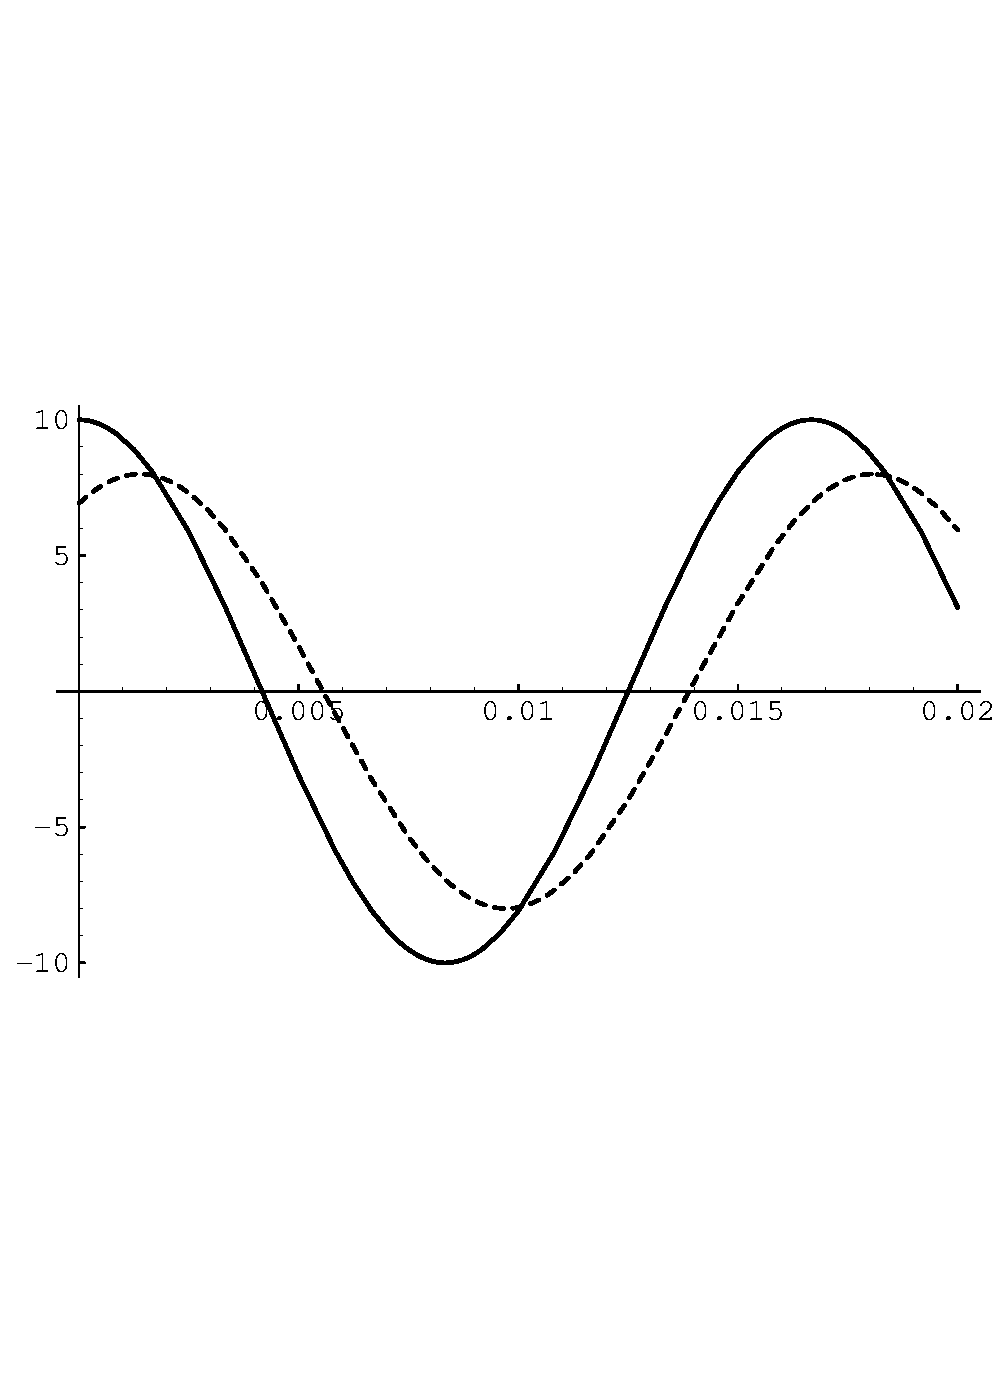
\epsfig{file=Figures/figure8.ps,height=5cm,bbllx=60pt,bblly=250pt,
bburx=550pt,bbury=530pt}
\caption{ \label{f:phaseF} This shows a driving voltage $V_{\rm coil}$
(solid curve) and the response voltage $V_{\rm IFO}$ (dotted curve) as
functions of time (in sec).  Both are 60 Hz sinusoids; the relative
amplitude and phase of the in-phase and out-of-phase components of
$V_{\rm IFO}$ are contained in the swept-sine calibration files.}
\end{center}
\end{figure}

We will shortly address the following question.  How does one use the
dimensionless data in the swept-sine calibration curve to reconstruct the
differential motion $\Delta l(t)$ (in meters) of the interferometer
arms?  Here we address the closely related question:  given $V_{\rm
IFO}$, how do we reconstruct $V_{\rm coil}$?  We choose the sign
convention for the Fourier transform which agrees with that of {\it
Numerical Recipes}:  equation (12.1.6) of \cite{NumRec}.  The Fourier
transform of a function of time $V(t)$ is
\begin{equation}
\label{e:fft1F}
{\tilde V}(f) = \int {\rm e}^{2 \pi i f t} V(t) dt.
\end{equation}
The inverse Fourier transform is
\begin{equation}
\label{e:fft2F}
V(t)= \int {\rm e}^{-2 \pi i f t} {\tilde V}(f) df.
\end{equation}
With these conventions, the signals (\ref{e:calibrate1F}) and
(\ref{e:calibrate2F}) shown in in Figure~\ref{f:phaseF} have Fourier
components:
\begin{eqnarray}
{\tilde V}_{\rm coil}(60) = 5                  \quad &{\rm and}& \quad {\tilde V}_{\rm coil}(-60) = 5,\\
{\tilde V}_{\rm IFO}(60)  = 4{\rm e}^{i \pi/6} \quad &{\rm and}& \quad {\tilde V}_{\rm IFO}(-60)  = 4 {\rm e}^{-i \pi/6}.
\end{eqnarray}
At frequency $f_0=60$ Hz the swept sine file
contains
\begin{equation}
S(60) = 0.8 \; {\rm e}^{-i \pi/6} \Rightarrow S(-60) = S^*(60) =
0.8 \; {\rm e}^{i \pi/6}.
\end{equation}
since $S(-f) = S^*(f)$.

With these choices for our conventions, one can see immediately from our
example (and generalize to all frequencies) that
\begin{equation}
\label{e:coilconF}
{\tilde V}_{\rm coil}(f) = {{\tilde V}_{\rm IFO} \over S^*(f)}.
\end{equation}
In other words, with the {\it Numerical Recipes} \cite{NumRec}
conventions for forward and reverse Fourier Transforms, the (FFT of
the) calibration-coil voltage is  the (FFT of the) IFO-output
voltage divided by the complex conjugate of the swept sine response.
\begin{description}
\item{Author:}  Bruce Allen, ballen@dirac.phys.uwm.edu
\item{Comments:}  The swept-sine calibration curves are usually quite
smooth but sometimes they contain a ``glitch" in the vicinity of
1 kHz; this may be due to drift of the unity-gain servo point.
\end{description}
\clearpage

\subsection{Function: {\tt GRcalibrate()}}
\label{ss:GRcalibrate}
\setcounter{equation}0
{\tt void GRcalibrate(float *fri,int frinum,int num,float *complex,float srate,int method,int order) }\\
This is a intermediate-level routine which 
takes as input a pointer to an array containing the swept sine data, and
outputs an array of interpolated points suitable for calibration of
FFT's of the interferometer output.

The arguments are:
\begin{description}
\item{\tt fri:} Input.  Pointer to an array containing
  swept sine data.  The format of this data is {\tt fri[0]=}$f_0$,
{\tt fri[1]=}$r_0$, {\tt fri[2]=}$i_0$,
{\tt fri[3]=}$f_1$,
{\tt fri[4]=}$r_1$, {\tt fri[5]=}$i_1$,... and the total length of the
array is {\tt fri[0..frinum-1]}.
\item{\tt frinum:} Input.  The number of entries in the array  {\tt fri[0..frinum-1]}.
If this number is not divisible by three, something is wrong!
\item{\tt num:} Input.  The number of points $N$ in the FFT that we
 will be calibrating.  This is typically $N=2^k$ where $k$ is an
 integer.  In this case, the number of distinct frequency values at
 which a calibration is needed is $2^{k-1}+1 = N/2+1$, corresponding to
 the number of distinct frequency values from $0$ (DC) to the Nyquist
 frequency $f_{\rm Nyquist}$.  See for example equation (12.1.5) of
 reference \cite{NumRec}.  The frequencies are $f_i = {i \over N}
 F_{\rm sample}$ for $i=0,\cdots,N/2$.
\item{\tt srate:} Input.  The sample rate $F_{\rm sample}$ (in Hz) of the data that
  we are going to be calibrating.
\item{\tt complex:} Input.  Pointer to an array {\tt complex[0..s]}
  where $s=2^k+1$.  The routine {\tt  calibrate()} fills in this array
  with interpolated values of the swept sine calibration data,
  described in the previous section.  The real part of the DC response
  is in {\tt complex[0]}, and the imaginary part is in {\tt
  complex[1]}. The real/imaginary parts of the response at frequency
  $f_1$ are in {\tt complex[2]} and {\tt complex[3]} and so on.  The
  last two elements of {\tt complex[ ]} contain the real/imaginary parts
  of the response at the Nyquist frequency $F_{\rm sample}/2$.
\item{\tt method:} Input.  This integer sets the type of interpolation
  used to determine the real and imaginary part of the response, at
  frequencies that lie in between those given in the swept sine
  calibration files.  Rational function interpolation is used if {\tt
  method}=0.  Polynomial interpolation is used if {\tt method}=1.
  Spline interpolation with natural boundary conditions (vanishing
  second derivatives at DC and the Nyquist frequency) is used if {\tt
  method}=2.
\item{\tt order:}  Input.  Ignored if spline interpolation is used.
  If polynomial interpolation is used, then {\tt order} is the order
  of the interpolating polynomial.
  If rational function interpolation is used, then the numerator and
  denominator are both polynomials of order {\tt order}/2 if {\tt order}
  is even; otherwise the degree of the denominator is ({\tt order}+1)/2
  and that of the numerator is ({\tt order}-1)/2.
\end{description}

The basic problem solved by this routine is that the swept sine
calibration data in a frame typically contain data at a few hundred
distinct frequency values.   However to properly calibrate the IFO output,
one usually needs this calibration information at a large number of
frequencies corresponding to the distinct frequencies associated with the
FFT of a data set.  This routine allows you to choose different possible
interpolation methods.  If in doubt, we recommend spline interpolation
as the first choice.  The interpolation methods are described in detail
in Chapter 3 of reference \cite{NumRec}.
\begin{description}
\item{Author:}  Bruce Allen, ballen@dirac.phys.uwm.edu
\item{Comments:}  It might be better to interpolate values of
$f^2$ times the swept-sine response function, as this is the quantity
needed to compute the IFO response function.
\end{description}
\clearpage

\subsection{Example: {\tt print\_ssF} program}
\label{ss:print_ssF}
\setcounter{equation}0
This example uses the function {\tt GRcalibrate()} to read the swept
sine calibration information from a frame, and then prints out a list
of frequencies, real, and imaginary parts interpolated from this data.
The frequencies are appropriate for the FFT of a 4096 point data set with
sample rate {\tt srate}.   The technique used is spline interpolation.
To run this program, and display a graph, type\\
\indent {\tt setenv GRASP\_FRAMEPATH /usr/local/GRASP/18nov94.1frame}\\
\indent {\tt print\_ssF > outputfile}\\
\indent {\tt xmgr -nxy outputfile}\\

\lgrindfile{Includes/print_ssF.tex}

\begin{figure}[h]
\begin{center}
\epsfig{file=Figures/swept.ps,angle=-90,bbllx=40pt,bblly=72pt,
bburx=580pt,bbury=720pt,width=5.0in}
\index{colorpage}
\caption{ \label{f:swept}
A swept sine calibration curve, showing the real and imaginary parts, produced by
the example program {\tt print\_ssF}.}
\end{center}
\end{figure}

\clearpage
\subsection{Function: {\tt GRnormalize()}}
\label{s:normalizeF}
\setcounter{equation}0
{\tt void GRnormalize(float *fri, int frinum, int npoint, float srate,float *response)}

This routine generates an array of complex numbers $R(f)$ from
the swept sine information in a frame, and an overall calibration
constant.  Multiplying this array of complex numbers by (the FFT of)
the raw IFO data yields the (FFT of the) differential displacement of
the interferometer arms $\Delta l$, in meters: $\widetilde{\Delta l}(f)
= R(f) \widetilde{C_{\rm IFO}}(f)$.  The units of $R(f)$ are meters/ADC-count.

The arguments are:
\begin{description}
\item{\tt fri:} Input.  Pointer to an array containing
  swept sine data.  The format of this data is {\tt fri[0]=}$f_0$,
{\tt fri[1]=}$r_0$, {\tt fri[2]=}$i_0$,
{\tt fri[3]=}$f_1$,
{\tt fri[4]=}$r_1$, {\tt fri[5]=}$i_1$,... and the total length of the
array is {\tt fri[0..frinum-1]}.
\item{\tt frinum:} Input.  The number of entries in the array  {\tt fri[0..frinum-1]}.
If this number is not divisible by three, something is wrong!
\item{\tt npoint:} Input.  The number of points $N$ of IFO output which will be used
to calculate an FFT for normalization.
Must be an integer power of 2.
\item{\tt srate:}  Input.  The sample rate in Hz of the IFO output.
\item{\tt response:} Output.  Pointer to an array {\tt response[0..s]}
with $s=N+1$ in which $R(f)$ will be returned.   By convention,
$R(0)=0$ so that {\tt response[0]=response[1]=0}.    Array elements
{\tt response[$2 i$]} and {\tt response[$2 i + 1$]} contain the real and
imaginary parts of $R(f)$ at frequency $f= i{\tt srate}/N$.   The
response at the Nyquist frequency {\tt response[N]=0} and {\tt
response[N+1]=0} by convention.
\end{description}

The absolute normalization of the interferometer can be obtained from
the information in the swept sine file, and one other normalization
constant which we denote by $Q$.  It is easy to understand how this
works.  In the calibration process, one of the interferometer end
mirrors of mass $m$ is driven by a magnetic coil.  The equation of
motion of the driven end mass is
\begin{equation}
m {d^2 \over dt^2} {\Delta l} = F(t)
\end{equation}
where $F(t)$ is the driving force and $\Delta l$ is the differential
length of the two interferometer arms, in meters.  Since the driving
force $d(t)$ is proportional to the coil current and thus to the coil
voltage, in frequency space this equation becomes
\begin{equation}
(- 2 \pi i f)^2 \widetilde{\Delta l}  = {\rm constant} \times \widetilde{V}_{\rm coil} =
{\rm constant} \times {{\tilde V}_{\rm IFO} \over S^*(f)}.
\end{equation}
We have substituted in equation (\ref{e:coilconF}) which relates
${\tilde V}_{\rm IFO}$ and ${\tilde V}_{\rm coil}$.
The IFO voltage is directly proportional to the quantity recorded in 
the IFO output channel: $V_{\rm IFO} = {\rm ADC} \times C_{\rm IFO}$, with the constant ${\rm ADC}$ 
being the ratio of the analog-to-digital converters input voltage to
output count.

Putting together these factors, the
properly normalized value of $\Delta l$, in meters, may be obtained
from the information in the IFO output channel, the swept sine calibration information, and the
quantities given in Table~\ref{t:unitsF} by
\begin{equation}
\label{e:rdefF}
\widetilde{\Delta  l} = R(f) \times \widetilde{C_{\rm IFO} }  \qquad {\rm with } \quad
R(f) = {Q  \times {\rm ADC}  \over -4 \pi^2 f^2 S^*(f)},
\end{equation}
where the $\tilde {}$ denotes Fourier transform, and $f$ denotes
frequency in Hz.  (Note that, apart from the complex conjugate on $S$,
the conventions used in the Fourier transform drop out of this
equation, provided that identical conventions
(\ref{e:fft1F},\ref{e:fft2F}) are applied to both $\Delta l$ and to
$C_{\rm IFO}$).
\begin{table}[h]
\caption{Quantities entering into normalization of the IFO output.}
\label{t:unitsF}
\begin{center}
\begin{tabular}[]{c|c|c|c}
Description            & Name      &  Value                & Units \\
\hline
Gravity-wave signal (IFO output)   & $C_{\rm IFO}$  &  varies               & ADC counts \\
\hline
A$\rightarrow$D converter sensitivity & ADC       &  10/2048              &    $ \rm V_{\rm IFO} \left({\rm ADC\ counts}\right)^{-1}      $ \\
\hline
Swept sine calibration & S(f)        &  from file            &  $   \rm V_{\rm IFO}  \left( V_{\rm coil}\right) ^{-1} $ \\
\hline
Calibration constant   &  $Q$      & $1.428\times 10^{-4}$ &  $ \rm meter\ Hz^2 \left(  V_{\rm coil} \right)^{-1} $
\end{tabular}
\end{center}
\end{table}
The constant quantity $Q$ indicated in the above equations has been
calculated and documented in a series of calibration experiments
carried out by Robert Spero. In these calibration experiments, the
interferometer's servo was left open-loop, and the end mass was driven
at a single frequency, hard enough to move the end mass one-half
wavelength and shift the interferences fringes pattern over by one
fringe.  In this way, the coil voltage required to bring about a given
length motion at a particular frequency was established, and
from this information, the value of $Q$ may be inferred.  During the
November 1994 runs the value of $Q$ was given by
\begin{equation}
Q = {\sqrt{9.35 \; \rm Hz} \over k} = 1.428 \times 10^{-4} {\rm
meter\ Hz^2 \over V_{\rm coil}} \qquad {\rm where\ } k=21399 {\rm
\ V_{\rm coil} \over meter \; Hz^{3/2}}.
\end{equation}

\begin{description}
\item{Author:}  Bruce Allen, ballen@dirac.phys.uwm.edu
\item{Comments:}  See comment for {\tt calibrate()}.
\end{description}
\clearpage

\subsection{Example: {\tt power\_spectrumF} program}
\label{ss:power_spectrumF}
\setcounter{equation}0
This example uses the function {\tt GRnormalize()} to produce a
normalized, properly calibrated power spectrum of the interferometer
noise, using the gravity-wave signal and the swept-sine calibration information
from the frames.

The output of this program is a 2-column file; the first column is
frequency and the second column is the noise in units of $\rm
meters/\sqrt{\rm Hz}$.
To run this program, and display a graph, type\\
\indent {\tt setenv GRASP\_FRAMEPATH /usr/local/GRASP/18nov94.1frame}\\
\indent {\tt power\_spectrumF > outputfile}\\
\indent {\tt xmgr -log xy outputfile}\\

\noindent
A couple of comments are in order here:
\begin{description}
\item{1.} 
Even though we only need the modulus, for pedagogic reasons, we explicitly
calculate both the real and imaginary parts of $\widetilde{\Delta l}(f)=
R(f) \widetilde{C_{\rm IFO}}(f)$.
\item{2.}
The fast Fourier transform of $\Delta l$, which we denote ${\rm
FFT}[\Delta l]$, has the same units (meters!) as $\Delta l$.  As can be
immediately seen from {\it Numerical Recipes} equation (12.1.6) the
Fourier transform $\widetilde{\Delta l}$ has units of meters-sec and is
given by $\widetilde{\Delta l} =\Delta t \; {\rm FFT}[\Delta l]$, where
$\Delta t$ is the sample interval.  The (one-sided) power spectrum of
$\Delta l$ in $\rm meters/\sqrt{\rm Hz}$ is $P=\sqrt{2 \over T}
| \widetilde{\Delta l} | $ where $T=N \Delta t$ is the total length of the
observation interval, in seconds.  Hence one has
\begin{equation}
P=\sqrt{2 \over N \Delta t} \; \Delta t \; | {\rm FFT}[\Delta l] |=
\sqrt{2 \Delta t \over N} \; | {\rm FFT}[\Delta l] |.
\end{equation}
This is the reason for the factor which appears in
this example.
\item{3.} To get a spectrum with decent frequency resolution, the time-domain
data must be windowed (see the example program {\tt calibrate} and the function
{\tt avg\_spec()} to see how this works).
\end{description}
A sample of the output from this program is shown in Figure~\ref{f:pspecF}.

\begin{figure}[hb]
\begin{center}
\index{colorpage}
\epsfig{file=Figures/figure9.ps,width=6in}
\caption{\label{f:pspecF} An example of a power spectrum curve produced
with {\tt power\_spectrumF}.  The spectrum produced off a data tape
(with 100 point smoothing) is compared to that produced by the HP
spectrum analyzer in the lab.}
\end{center}
\end{figure}
\lgrindfile{Includes/power_spectrumF.tex}

\begin{description}
\item{Author:}
Bruce Allen, ballen@dirac.phys.uwm.edu
\item{Comments:}
The IFO output typically consists of a number of strong line sources
(harmonics of the 60 Hz line and the 180 Hz laser power supply, violin
modes of the suspension, etc) superposed on a continuum background
(electronics noise, laser shot noise, etc)  In such situations, there
are better ways of finding the noise power spectrum (for example, see the
multi-taper methods of David J. Thompson \cite{thomson82}, or the textbook
by Percival and Walden \cite{percivalwalden}). Using methods such as the
F-test to remove line features from the time-domain data stream might
reduce the sidelobe contamination (bias) from nearby frequency bins,
and thus permit an effective reduction of instrument noise near these
spectral line features.  Further details of these methods, and some
routines that implemen them, may be found in Section~\ref{ss:mtapintro}.
\end{description}
\clearpage

\subsection{Example: {\tt calibrateF} program}
\setcounter{equation}0
This example uses the function {\tt GRnormalize()} and {\tt
avg\_spec()} to produce an animated display, showing the properly
normalized power spectrum of the interferometer, with a 30-second
characteristic time moving average.  After compilation, to run the
program type:\\
\indent {\tt setenv GRASP\_FRAMEPATH /usr/local/GRASP/18nov94.1frame}\\
\indent {\tt calibrateF $|$ xmgr -pipe \&} \\
to get an animated display showing the calibrated power spectrum
changing.  An example of the output from {\tt calibrateF} is shown in
Figure~\ref{f:calibrateF}.  Note that most of the execution time here is
spent passing data down the pipe to {\tt xmgr} and displaying it.  The
display can be speeded up by a factor of ten by binning the
output values to reduce their number to a few hundred lines (the example
program {\tt calibrate\_binnedF.c} implements this technique; it can be
run by typing {\tt calibrate\_binnedF | xmgr -pipe}).

\begin{figure}[hb]
\index{colorpage}
\begin{center}
\epsfig{file=Figures/figure11.ps,width=6in}
\caption{\label{f:calibrateF} 
This shows a snapshot of the output from the program {\tt calibrateF}
which displays an animated average power spectrum (Welch windowed, 30-second decay time).}
\end{center}
\end{figure}

\lgrindfile{Includes/calibrateF.tex}

\begin{description}
\item{Author:}
Bruce Allen, ballen@dirac.phys.uwm.edu
\item{Comments:}
See comments for {\tt power\_spectrumF} example program.
\end{description}
\clearpage

\subsection{Example: {\tt transferF} program}
\setcounter{equation}0
This example uses the function {\tt GRnormalize()} to calculate the
response of the interferometer to a specified gravitational-wave strain
$h(t)$. [Note: for clarity, in this example, we have NOT worried about
getting the overall normalization correct.] The code includes two
possible $h(t)$'s.  The first of these is a binary-inspiral chirp (see
Section~\ref{s:inspiral}).  Or, if you un-comment one line of code, you
can see the response of the detector to a unit-impulse gravitational
wave strain, in other words, the impulse response of the detector.

Note that to run this program, you must specify
a path to the 40-meter data, for example by typing:\\
\indent {\tt setenv GRASP\_FRAMEPATH /usr/local/data/19nov94.3.frame}\\ 
so that the code can find a frame containing a swept-sine calibration
file to use.

The response of the detector to a pair of inspiraling stars is shown in
Figure~\ref{f:detrespF}.  You will notice that although the chirp starts at
a (gravitational-wave) frequency of 140 Hz on the left-hand side of the
figure, the low-frequency response of the detector is so poor that the
chirp does not really become visible until about half-a-second later,
at somewhat higher frequency.  In the language of the audiophile, the
IFO has crummy bass response!  Of course this is entirely deliberate;
the whitening filters of the instrument are designed to attenuate the
low-frequency seismic contamination, and consequently also attenuate
any possible low-frequency gravitational waves.

\begin{figure}[hb]
\begin{center}
\epsfig{file=Figures/transfer.ps,angle=-90,width=5in}
\caption{\label{f:detrespF}
Output produced by the {\tt transfer} example program.
The top graph shows the gravitational-wave strain produced by an
inspiraling binary pair.  The lower graph shows the calculated
interferometer output [channel.0  or IFO\_DMRO] produced by this
signal.  Notice that because of the poor low-frequency response of the
instrument, the IFO output does not show significant response before
the input frequency has increased.  The sample rate is slightly under
10 kHz.
}
\end{center}
\end{figure}

The response of the detector to a unit gravitational strain impulse is
shown as a function of time-offset in Figure~\ref{f:detresp2F}.  Here
the predominant effect is the ringing of the anti-aliasing filter.  The
impulse response of the detector lasts about 30 samples, or 3 msec.
For negative offset times the impulse response is quite close to zero;
its failure to vanish is partly a wrap-around effect, and partly due to
errors in the actual measurement of the transfer function.

\begin{figure}[hb]
\begin{center}
\epsfig{file=Figures/impulse.ps,angle=-90,width=4in}
\caption{\label{f:detresp2F}
Output produced by the {\tt transfer} example program.
This shows the calculated
interferometer output [channel.0  or IFO\_DMRO] produced by
an impulse in the gravitational-wave strain at sample number zero.
This (almost) causal impulse response lasts about 3 msec.
}
\end{center}
\end{figure}

This is a good place to insert a cautionary note.  Now that we have
determined the transfer function $R(f)$ of the instrument, you might be
tempted to ask: ``Why should I do any of my analysis in terms of the
instrument output?  After all, my real interest is in gravitational
waves.  So the first thing that I will do in my analysis is convert the
instrument output into a gravitational wave strain $h(t)$ at the
detector, by convolving the instrument's output with (the time-domain
version of) $R(f)$."  {\bf Please do not make this mistake!} A few moment's
reflection will show why this is a remarkably bad idea.  The problem
is that the response function $R(f)$ is extremely
large at low frequencies.  This is just a reflection of the poor low
frequency response of the instrument: any low-frequency energy in the
IFO output corresponds to an extremely large amplitude low frequency
gravitational wave.  So, if you calculate $h(t)$ in the way described:
take a stretch of (perhaps zero-padded) data, FFT it into the frequency domain,
multiply it by $R(f)$ and invert the FFT to take it back into the frequency
domain, you will discover the following:
\begin{itemize}
\item
Your $h(t)$ is dominated by a single low-frequency noisy sinusoid
(whose frequency is determined by the low frequency cutoff imposed by
the length of your data segment or the low-frequency cutoff of the
response function).
\item
Your $h(t)$ has {\it lost} all the interesting information present at
frequencies where the detector is quiet (say, around 600 Hz).  Because
the noise power spectrum (see Figure~\ref{f:pspecF}) covers such a large
dynamic range, you can not even represent $h(t)$ in a floating point
variable (though it will fit, though barely, into a double).  This is
why the instrument uses a whitening filter in the first place.
\item
It is possible to construct ``$h(t)$" if you filter out the
low-frequency garbage by setting $R(f)$ to zero below (say) 100 Hz.
\end{itemize}
If you are unconvinced by this, do the following exercise:  calculate
the power spectrum in the frequency domain as was done with
Figure~\ref{f:pspecF}, then construct $h(t)$ in time time domain, then
take $h(t)$ back into the frequency domain, and graph the power
spectrum again.  You will discover that it has completely changed above
100 Hz and is entirely domainted by numerical quantization noise
(round-off errors).

\lgrindfile{Includes/transferF.tex}

\begin{description}
\item{Author:}
Bruce Allen, ballen@dirac.phys.uwm.edu
\item{Comments:}
None.
\end{description}
\clearpage

\subsection{Example: {\tt diagF} program}
\setcounter{equation}0
This program is a frequency-domain ``novelty detector" and provides a
simple example of a time-frequency diagnostic method.  
The actual code is not printed here, but may be found in the GRASP directory
\linebreak[4]
\texttt{src/examples/examples\_frame} in the file {\tt diagF.c}. To run the
program type:\\
\indent {\tt setenv GRASP\_FRAMEPATH /usr/local/GRASP/18nov94.1frame}\\
\indent {\tt diagF \&} \\
which will start the {\tt diagF} program in the background.

The method used by {\tt diagF} is as follows:
\begin{enumerate}
\item
A buffer is loaded with a short stretch of data samples (2048 in this
example, about 1/5 of a second).
\item
A (Welch-windowed) power spectrum is calculated from the data in 
the buffer.  In each frequency bin,
 this provides a value $S(f)$.
\item
Using the same auto-regressive averaging technique described in {\tt
avg\_spec()} the mean value of $S(f)$ is maintained in a time-averaged
spectrum $\langle S(f) \rangle$.  The exponential-decay time constant
for this average is {\tt AVG\_TIME} (10 seconds, in this example).
\item
The absolute difference between the current spectrum and the average
$\Delta S(f) \equiv |S(f) - \langle S(f) \rangle |$ is determined. Note
that the absolute value used here provides a more robust first-order
statistic than would be provided by a standard variance $(\Delta
S(f))^2$.
\item
Using the same auto-regressive averaging technique described in {\tt
avg\_spec()} the value of $\Delta S(f)$ is maintained in a
time-averaged absolute difference $\langle \Delta S(f) \rangle$.  The
exponential-decay time constant for this average is also set by {\tt
AVG\_TIME}.
\item
In each frequency bin, $\Delta S(f)$ is compared to $\langle \Delta
S(f) \rangle$.  If $\Delta S(f) > {\tt THRESHOLD} \times \langle \Delta
S(f) \rangle$ then a point is plotted for that frequency bin; otherwise
no point is plotted for that frequency bin.  In this example, {\tt
THRESHOLD} is set to 6.
\item
In each frequency bin, $\Delta S(f)$ is compared to $\langle \Delta
S(f) \rangle$.  If $\Delta S(f) < {\tt INCLUDE} \times \langle \Delta
S(f) \rangle$ then the values of $S(f)$ and $\Delta S(f)$ are used to
``refine" or ``revise" the auto-regressive means described previously.
In this example, {\tt INCLUDE} is set to 10.
\item
Another set of points (1024 in this example) is loaded into the
end of the buffer, pushing out the oldest 1024 points from the start
of the buffer, and the whole loop is restarted at step 2 above.
\end{enumerate}
The {\tt diagF} program can be used to analyze any of the different
channels of fast-sampled data, by setting {\tt CHANNEL}
appropriately.  It creates one output file for each locked segment of
data.  For example if {\tt CHANNEL} is set to 0 (the IFO channel)
and there are four locked sections of data, one obtains a set of
files:\\
{\tt ch0diag.000}, 
{\tt ch0diag.001}, 
{\tt ch0diag.002}, and
{\tt ch0diag.003}.\\
In similar fashion, if {\tt CHANNEL} is set to 1 (the magnetometer)
one obtains files:\\
{\tt ch1diag.000}, 
{\tt ch1diag.001}, 
{\tt ch1diag.002}, and
{\tt ch1diag.003}.\\
These files may be used as input to the {\tt xmgr} graphing program,
by typing:\\
{\tt xmgr ch0diag.000 ch1diag.000}\\
(one may specify as many channels as desired on the input line).  A
typical pair of outputs is shown in Figures~\ref{f:diag0F} and
\ref{f:diag1F}.  By specifying several different channels on the command
line for starting {\tt xmgr}, you can overlay the different channels
output with one another.  This provides a visual tool for identifying
correlations between the channels (the graphs shown below may be
overlaid in different colors).
\begin{description}
\item{Author:}
Bruce Allen, ballen@dirac.phys.uwm.edu
\item{Comments:}
This type of time-frequency event detector appears quite useful as a
diagnostic tool.  It might be possible to improve its high-frequency
time resolution by being clever about using intermediate information
during the recursive calculation of the FFT.  One should probably also
experiment with using other statistical measures to assess the behavior
of the different frequency bins.  It would be nice to modify this
program to also examine the slow sampled channels (see comment for {\tt
get\_data()}).
\end{description}
\begin{figure}[t]
\begin{center}
\epsfig{file=Figures/figure13a.ps,angle=-90,width=5in}
\caption{ \label{f:diag0F} A time-frequency diagnostic graph produced by
{\tt diag}.  The vertical line pointed to by the arrow is a
non-stationary noise event in the IFO output, 325 seconds into the
locked section.  It sounds like a ``drip" and might be due to off-axis
modes in the interferometer optical cavities.}
\end{center}
\end{figure}
\begin{figure}[b]
\index{colorpage}
\begin{center}
\epsfig{file=Figures/figure13b.ps,angle=-90,width=5in}
\caption{ \label{f:diag1F} A time-frequency diagnostic graph
produced by {\tt diag}.  This shows the identical period as the previous
graph, but for the magnetometer output.  Notice that the spurious event
was not caused by magnetic field fluctuations.}
\end{center}
\end{figure}
\clearpage

\subsection{Example: {\tt seismicF} program}

This is an example program which produces power spectra of seismometer
ground motion.  It is intended for use with a Guralp CMG-40T Broadband
Seismometer \htmladdnormallink{{\tt http://www.guralp.demon.co.uk/}}
{http://www.guralp.demon.co.uk/}, with the velocity sensing output set for the $0.033\rightarrow100$Hz band and the gain set to 400 volts-sec/meter.
The normalization constants are defined with a line that reads
something like this.
\begin{verbatim}
const float norm=((0.25/65536.0)*(1.0/400.0)*(1.0/(2.0*M_PI)));
\end{verbatim}
Here the constants assume that the ADC that the seismometer is connected to
records 65536 ADC counts per $0.25$~volts input and that
the gain (single-ended) is set to 400~volts-sec/meter. The $2\pi$ and a
factor of frequency $f$ arise in the code in converting velocity to position.
The program outputs postscript and/or jpeg files labeled by GPS time.
\begin{figure}[h]
\index{colorpage}
\begin{center}
\epsfig{file=Figures/Spec.610452023.ps,height=5.5in}
\caption{ \label{f:seismicF} \small
A seismometer (one-sided) power spectrum produced by the {\tt seismicF}
example program.  The x,y, and z (vertical) motion are shown in
black, red, and green.  The blue curve shows the LIGO standard noise
power spectrum, for comparison.  This spectrum was taken at the LIGO
Hanford site, during the installation.  The portable clean rooms
may be responsible for much of the excess noise.  The file name
is {\tt Spec.610452023.ps}}
\end{center}
\end{figure}




% GRASP: Copyright 1997,1998,1999  Bruce Allen %
% $Id: man_correlation.tex,v 1.4 1999/07/11 21:22:10 ballen Exp $
\section{GRASP Routines: Signal-to-noise enhancement techniques}
\label{s:correlation}
\setcounter{equation}0

\subsection{Signal-to-noise enhancement by environmental cross-correlation}
\setcounter{equation}0
\label{ss:cross-correlation}

There are many situations of interest in which data are contaminated
by the environment.  Often this contamination is understood, and by
monitoring the environment it is possible to ``clean up" or ``reduce"
the data, by subtracting the effects of the environment from the
signal or signals of interest.  In the case of the data stream from an
interferometric gravitational radiation detector, the signal of
interest is the differential displacement of suspended
test masses.  This displacement arises from gravitational waves but
also has contributions arising from other contaminating sources, such
as the shaking of the optical tables (seismic noise) and forces due to
ambient environmental magnetic fields.  The key point is that the
gravitational waves are not correlated with any of these environmental
artifacts.

The method implemented here works by estimating the linear transfer
function between the IFO\_DMRO channel and specified environmental
channels on the basis of the correlations over a certain bandwidth in
Fourier space.  The method is explained in detail in the paper
`\emph{Automatic cross-talk removal from multi-channel data}'
(WISC-MILW-99-TH-04)%
\footnote{available from
\htmladdnormallink{{\tt http://www.lsc-group.phys.uwm.edu/$\sim$www/docs/pub\_table/gravpub.html}}
{http://www.lsc-group.phys.uwm.edu/~www/docs/pub_table/gravpub.html}
.}
Here we will just give a very brief overview to introduce the quantities calculated.

We denote the channel of interest, normally the InterFerOmeter Differential
Mode Read-out (IFO\_DMRO), by $X$ or $Y_1$.  The other sampled channels consist
of environmental and instrumental monitors which we denote
$Y_2,\dots,Y_N$.  We assume that all fast channels have been decimated
so that all channels are sampled at the same (slow) rate,
$986.842\cdots\ $Hz for the November 1994 40-meter data.


We assume that the contribution of channel $i$ to channel $1$ is
described by an (unknown!) linear transfer function $R_i(t-t')$. The
basic idea of the method is to use the data to estimate the transfer
functions $R_i$.  For the reasons discussed in the paper, we work
with the data in Fourier space.  The transfer function is estimated by
averaging over a frequency band, that is a given number of frequency
bins.  The number of bins in any band is  denoted by $F$ in
the cited paper and {\tt correlation\_width} in
the programs below.  The method assumes that $\tilde R_i$ can be well
approximated by a {\it complex constant} within each frequency band,
in other words that the transfer function
does not vary rapidly over the frequency bandwidth $\Delta f = F/T$
where $T$ is total time of the data section under consideration.
The choices 32, 64 and 128 appear most appropriate for $F$ for the
40-meter data. 

Within a given band, $b$, the Fourier components of the field may be thought
of as the components of an $F$-dimensional vector, ${\bf Y}_i^{(b)}$.    
Correlation between two channels (or the auto-correlation of
a channel with itself) may be expressed by the standard inner product
$({\bf Y}_i^{(b)},{\bf Y}_j^{(b)}) = {\bf Y}_i^{(b)}{\cdot}{\bf
  Y}_j^{(b)*}$ (no summation over $b$). Our assumption that $\tilde R_i$
is constant over each band means that the `true' channel of interest
(the IFO\_DMRO channel with environmental influences subtracted) can
be written
\begin{equation}
\bar {\tilde {\bf x}}^{(b)} =  {\tilde {\bf X}}^{(b)} - \sum_{j=2}^N
r^{(b)}_j {\tilde {\bf Y}_j}^{(b)}.
\end{equation}
where $r^{(b)}_j$, $j=2,\dots,N$ are constants.
The fundamental assumption is that the best estimate of the transfer
function in the frequency band $b$ is given by the complex vector 
$(r^{(b)}_2,\dots,r^{(b)}_N)$ that minimises 
$|\bar {\tilde {\bf x}}^{(b)}|^2$.
To measure the `improvement' in the signal we define $|\rho|^2$ by
\begin{equation}
 |\bar {\tilde {\bf x}}^{(b)}|^2 = | {\tilde {\bf X}}^{(b)}|^2 
      \left( 1 - |\rho|^2 \right) .
\end{equation}
denoted by {\tt rho2} in the programs below.
By definition $0 \leq |\rho|^2 \leq 1$.
If any of the  environmental channels are strongly correlated
with the channel of interest, a significant reduction in  
$|\bar {\tilde {\bf x}}^{(b)}|^2$ is
obtained, that is, $|\rho|^2$ will be close to 1.

To understand the origin of the `improvement' it is also convenient to
study the best estimate that can be obtained using any given single
environmental channel.  Thus we define 
\begin{equation}
\bar {\tilde {\bf x}}^{(b)}_i
=  {\tilde {\bf X}}^{(b)} - 
{r'}^{(b)}_i {\tilde {\bf Y}_i}^{(b)}
\end{equation}
and choose the complex number ${r'}^{(b)}_i$ to  minimise 
$|\bar {\tilde {\bf x}}^{(b)}_i|^2$.  Of course, in general this
will not correspond to the $i$th component of the vector 
used in the multi-channel case.
The corresponding improvement $|\rho_i|^2$ given by 
\begin{equation}
|\bar {\tilde {\bf x}}^{(b)}_i|^2 = |{\tilde {\bf X}}^{(b)}|^2 
      \left( 1 - |\rho_i|^2 \right)
\end{equation}
is denoted by {\tt rho2\_pairwise} in the programs below.
By definition $0 \leq |\rho_i|^2 \leq 1$.
If the $i$th  environmental channel is  strongly correlated
with the channel of interest, a significant reduction in  
$|\bar {\tilde {\bf x}}^{(b)}_i|^2$ is
obtained, that is, $|\rho_i|^2$ will be close to 1.
 



\clearpage
\subsection{Outline}

Calculation of environmental correlations using the routines presented
in this chapter proceeds through the 
establishment of a configuration file, called here {\tt 40m.config} 
with the following structure:

\begin{verbatim}
#  Correlations between 40m Channels  over a period
#  of approximately 266 seconds. The IFO sample rate is 
#  9868.4\dots Hz (hence 9868.4 x 266 = 2621440 samples).
#  The sample rate for the `slow' channels is
#  (1/10)th that of the `fast' so (1/10)th the
#  number of samples are requested 
C1
4
IFO_DMRO        S        2621440
IFO_Mike        S        2621440
IFO_Seis_1      S        262144
IFO_SPZT        S        262144
1
\end{verbatim}

  The file may {\it begin} with any number of comment lines beginning
with an initial {\tt \#}.  The next line is a character string 
describing the detector, this is just used for naming intermediate files.
The following line gives the total number of channels (signal plus
environmental).  There follow this number of lines each containing
three columns, the first of these lines pertains to the signal 
the remainder to environmental channels.  The three columns are:
\begin{enumerate}
\item the name of the channel,
\item the data type of the channel (here short) -- see {\tt
animateT.c} or {\tt corr\_init.c} for a description of the possible types,
and 
\item the number of data points from that channel to be analysed --
these should correspond to the same period of time.
\end{enumerate}


\noindent Finally, there is a line containing a single number.  This should be
set to 1 if the user wants to obtain `cleaned' output and 0 if the
user just wants to see correlation data.  (Note: This line is not used by
{\tt corr\_init} described below, but only by {\tt env\_corr}.  Thus it
is possible to change one's mind about whether to find the cleaned 
signal without having to rerun {\tt corr\_init}.)

The configuration file is used by the two basic programs:
\begin{enumerate}
\item {\tt  corr\_init} which calculates the Fourier transforms and writes 
binary data files in a data directory named {\tt `configuration name'\_fft}, so
{\tt 40m\_fft} in the above example. Only those frequencies
appropriate to the slowest channel are saved.
\item {\tt env\_corr} which calculates the correlations between each
environmental channel and the signal channel and pops up a graph 
of these correlations.  
The data for this graph is stored in the same data directory as the
FFT data.  {\tt env\_corr} also produces a file {\tt corr\_view\dots}
which enables this graph to be reproduced later without running  {\tt
  env\_corr} again.  If the configuration file asks for the
signal to be cleaned {\tt env\_corr} will also produce an ASCII data file
giving the (FFT of the) `cleaned' signal and also the total fractional reduction 
in noise obtained by the method. 
Again this file is stored in the same data directory, its first line
gives the frequency spacing and the following lines the real and
imaginary parts of the FFT of the cleaned signal.  (To avoid plotting
difficulties with {\tt xmgr} the DC component is arbitrarily set equal
to that of the first bin.)  
\end{enumerate}

Thus, having created the appropriate configuration file one would
type {\tt corr\_init  40m.config} and then {\tt env\_corr 40m.config}.
(Of course, the environment variable {\tt GRASP\_FRAMEPATH} must first
be set to the directory containing the appropriate frames.)

\begin{description}
\item{Note:} These programs perform linear algebra by calls to 
{\tt clapack} routines.  These may be obtained from {\tt
  http://www.netlib.org/}.  These routines use {\tt f2c} 
and, in particular, use complex numbers defined
in {\tt f2c.h} through the structure:

{\tt 
typedef struct \{\\
  float r;  /* real part */\\
  float i;  /* imaginary part */\\
\} complex;}

\end{description}

\clearpage
\subsection{Function: {\tt calc\_rho()}}
\setcounter{equation}0
{\tt int calc\_rho(int offset,int correlation\_width,float threshold,
               float *rp\_signal,\\float *ip\_signal,int nenv\_chan,
               float **rp\_env,float **ip\_env,\\ float *rho2\_pairwise,
               complex *A,complex *B,float *modx2sum)} 

This function takes sections of length {\tt length} of the Fourier
transform of the `signal' channel and {\tt nenv\_chan} environmental
channels and estimates the transfer function on the basis of
correlations over a width  of {\tt correlation\_width} bins at an
offset frequency of {\tt offset} bins.  It returns an array {\tt rho2\_pairwise}
containing the values of $|\rho|^2$ that would arise from a
cross-correlation with each single channel thereby giving information
on {\it which}
environmental channels contain the strongest evidence for correlation with 
the signal.

The arguments are:
\begin{description}
\item{\tt length:} Input. The total length of the Fourier transform.
\item{\tt offset:} Input. The offset to the beginning of the section
  of the Fourier transform over which correlations are being searched for.
\item{\tt correlation\_width:} Input.  The width of the section
  of the Fourier transform over which correlations are being searched for.
\item{\tt threshold:} Input. The threshold for determining whether a
correlation is statistically significant.
\item{\tt rp\_signal:} Input. {\tt  rp\_signal[0..length-1]} contains the
  real parts of the Fourier transform of the signal.
\item{\tt ip\_signal:} Input. {\tt  ip\_signal[0..length-1]} contains the
  imaginary parts of the Fourier transform of the signal.
\item{\tt nenv\_chan:} Input. The number of environmental channels under
  consideration.
\item{\tt rp\_env:} Input. {\tt  rp\_env[0..nenv\_chan-1][0..length-1]} contains the
  real parts of the Fourier transform of the nenv\_chan environmental channels.
\item{\tt ip\_env:} Input. {\tt  ip\_env[0..nenv\_chan-1][0..length-1]} contains the
  imaginary parts of the Fourier transform of the nenv\_chan environmental
  channels.
\item{\tt rho2\_pairwise:} Output. {\tt rho2\_pairwise[0..nenv\_chan-1]} contain
  the level of {\it pairwise} correlation between  the signal and each
  environmental channel in turn, {\it i.e.}, the value of $|\rho|^2$ 
  obtained if just the $i$th environmental channel had been used.
\item{\tt A:} Input/Output. {\tt A[0..${\tt nenv\_chan}^2$-1]} is a working
  array that is used by the {\sl clapack} routine {\tt chesv()} called by {\tt clean\_chan()}.  
  The elements of the array are structure of type {\tt complex} (see
  note above).  Memory allocation should be performed in the
  calling routine.
\item{\tt B:} Input/Output. {\tt B[0..${\tt nenv\_chan}$-1]} is a working
  array used by the {\sl clapack} routine {\tt chesv()} called by {\tt clean\_chan()}.  
  The elements of the array are structure of type {\tt complex} (see
  note above).  Memory allocation should  be performed in the
  calling routine.
\item{\tt modx2sum:} Output.  A float used by {\tt clean\_chan}.
\end{description}

\begin{description}
\item{Author:}
Bruce Allen (ballen@dirac.phys.uwm.edu), Wensheng Hua (hua@bondi.phys.uwm.edu)
  and Adrian Ottewill (ottewill@relativity.ucd.ie).
\item{Comments:}

\end{description}
\clearpage

\subsection{Function {\tt chan\_clean()}}

\setcounter{equation}0

{\tt int chan\_clean(int offset,int correlation\_width,float
  threshold,float *rho2,\\
float *rp\_signal,float *ip\_signal,
               int nenv\_chan,float **rp\_env,float **ip\_env,\\
float *rp\_clean,float *ip\_clean,complex *A,complex *B,\\
               float modx2sum,complex *R,complex *work,integer lwork,integer *ipivot)}

\begin{description}
\item{Note:} The data type {\tt integer} is defined in {\tt f2c.h}.
\end{description}

\begin{description}
\item{\tt offset:} Input. The offset to the beginning of the section
  of the Fourier transform over which correlations are being searched for.
\item{\tt correlation\_width:} Input.  The width of the section
  of the Fourier transform over which correlations are being searched for.
\item{\tt threshold:} Input. The threshold for determining whether a
correlation is statistically significant.
\item{\tt rp\_signal:} Input. {\tt  rp\_signal[0..length-1]} contains the
  real parts of the Fourier transform of the signal.
\item{\tt ip\_signal:} Input. {\tt  rp\_signal[0..length-1]} contains the
  imaginary parts of the Fourier transform of the signal.
\item{\tt nenv\_chan:} Input. The number of environmental channels under
  consideration.
\item{\tt rp\_env:} Input. {\tt  rp\_env[0.. nenv\_chan-1][0..length-1]} contains the
  real parts of the Fourier transform of the nenv\_chan environmental channels.
\item{\tt ip\_env:} Input. {\tt  ip\_env[0.. nenv\_chan-1][0..length-1]} contains the
  imaginary parts of the Fourier transform of the nenv\_chan environmental
  channels.
\item{\tt rp\_clean:} Output. {\tt  rp\_clean[0..length-1]} contains the
  real parts of the Fourier transform of the signal cleaned by
  removing those contributions that have been assigned by the method
  to environmental influences.
\item{\tt ip\_clean:} Output. {\tt  ip\_clean[0..length-1]} contains the
  imaginary parts of the Fourier transform of the signal cleaned by
  removing those contributions that have been assigned by the method
  to environmental influences.
\item{\tt A:} Input. {\tt A[0..${\tt nenv\_chan}^2$-1]} is a working
  array that is calculated by {\tt calc\_rho()} and used by the {\sl
  clapack} routine {\tt chesv()} called by {\tt clean\_chan()}.  
  The elements of the array are structure of type {\tt complex} (see
  note above).  Memory allocation should be performed in the
  calling routine.
\item{\tt B:} Input. {\tt B[0..${\tt nenv\_chan}$-1]} is a working
  array that is calculated by {\tt calc\_rho()} used by the {\sl
    clapack} 
routine {\tt chesv()} called by {\tt clean\_chan()}.  
  The elements of the array are structure of type {\tt complex} (see
  note above).  Memory allocation should  be performed in the
  calling routine.
\item{\tt modx2sum:} Input.  A float that is calculated by {\tt
    calc\_rho} used by {\tt clean\_chan}.
\item{\tt R:} Input. {\tt R[0..${\tt nenv\_chan}$-1]} is a working
  array used by the {\sl clapack} routine {\tt chesv()} called by {\tt clean\_chan()}.  
  The elements of the array are structure of type {\tt complex} (see
  note above).  Memory allocation should be performed in the
  calling routine. 
\item{\tt work:} Input. {\tt work[0..${\tt lwork}$-1]} is a working
  array used by the {\sl clapack} routine {\tt chesv()} called by {\tt clean\_chan()}.  
  The elements of the array are structure of type {\tt complex} (see
  note above).  Memory allocation should be performed in the
  calling routine. 
\item{\tt lwork:} Input. The size of the array {\tt work}.
\item{\tt ipivot:} Input. {\tt ipivot[0..${\tt nenv\_chan}$-1]} is a working
  array used by the {\sl clapack} routine {\tt chesv()} called by {\tt clean\_chan()}.  
  The elements of the array are structure of type {\tt integer}.  Memory
  allocation should be performed in the  calling routine. 
\end{description}
\begin{description}
\item{Author:}
Bruce Allen (ballen@dirac.phys.uwm.edu), Wensheng Hua (hua@bondi.phys.uwm.edu)
  and Adrian Ottewill (ottewill@relativity.ucd.ie).
\item{Comments:}
{\tt clean\_chan()} currently uses {\sl clapack} routines to
perform the required matrix manipulations.  While this it is highly
desirable to have such optimised routines when considering a large
number of environmental channels it would also be useful to have a replacement
for the {\sl clapack} routine {\tt chesv()} constructed from Numerical
Recipes routines for when {\sl clapack} is not available.
\end{description}

\clearpage




\subsection{Example: Correlations in data from the  40m interferometer }


 

The output below was produced starting with  2621440 samples from the 19
November 1994 run 3 data set, covering about 266 seconds.

The fast channels, including the IFO\_DMRO channel, were decimated
so that all channels are effectively sampled at the slow channel rate
of $986.842\dots\,$Hz. This yields a (real) time series with 262144
samples and correspondingly a (complex) FFT of length 131072 as
specified by the macro name {\tt LENGTH}.
Averaging is carried out over 128 frequency bins but this may
be varied to include a range of bandwidths  {\tt MIN\_BANDWIDTH} and {\tt MAX\_BANDWIDTH}. 

\begin{figure}[ht]
\index{colorpage}
\begin{center}
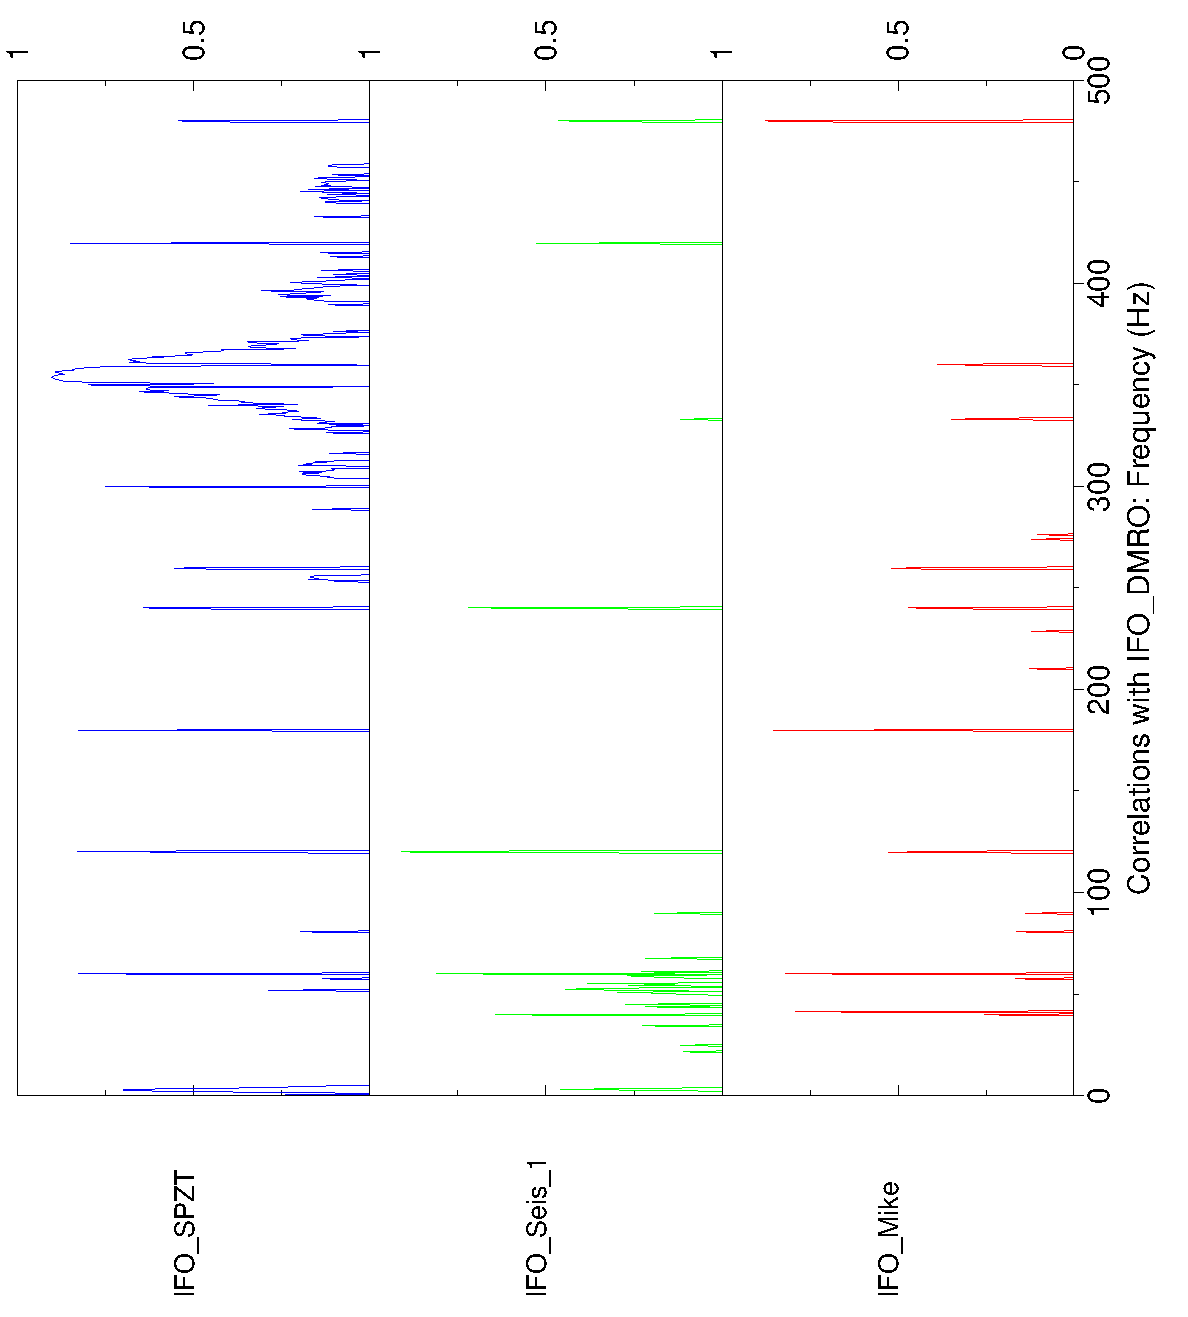
\epsfig{file=Figures/xmgr.eps,angle=270,width=5in}
\caption{ \label{f:rho2} The graphical display of the contents of the 
output file  {\tt 40m\_fft/rho2\_IFO\_128.dat} produced by {\tt env\_corr}
illustrating strong environmental cross-correlation.  
 The three graphs show the correlation between the
IFO\_DMRO channel and each individual environmental channel.
This graph is produced by the file {\tt corr\_view128} which {\tt
  env\_corr} produces.}

\end{center}
\end{figure}


The output was obtained from the commands

\centerline{\tt corr\_init 40m.config}

\noindent followed by

\centerline{\tt env\_corr 40m.config}

\noindent where  {\tt 40m.config} is the configuration file printed above.
This corresponding to seeking correlations between the
interferometer output (IFO\_DMRO) channel and 
\begin{description}
\item{IFO\_Mike:} The microphone output.
\item{IFO\_Seis\_1:} The seismometer output.
\item{IFO\_SPZT:} The slow pzt.
\end{description}

The data below show sections of the output file  {\tt 40m\_fft/rho2\_IFO\_128.dat}
illustrating strong environmental cross-correlation
at around $40$Hz with the seismometer and microphone output, at 
around $120$Hz with all three channels, and in a broad band 
around 360Hz with the slow pzt.

{\tt 
\begin{verbatim}
... 
39.271          0.000           0.000 0.000 0.000 
39.753          0.654           0.256 0.644 0.000 
40.235          0.000           0.000 0.000 0.000 
40.717          0.000           0.000 0.000 0.000 
41.199          0.794           0.794 0.000 0.000 
41.681          0.000           0.000 0.000 0.000 
...
118.778         0.000           0.000 0.000 0.000 
119.259         0.000           0.000 0.000 0.000 
119.741         0.940           0.528 0.876 0.519 
120.223         0.973           0.371 0.911 0.830 
120.705         0.000           0.000 0.000 0.000 
121.187         0.000           0.000 0.000 0.000 
...
352.478         0.886           0.000 0.000 0.886 
352.960         0.897           0.000 0.000 0.897 
353.442         0.899           0.000 0.000 0.899 
353.924         0.904           0.000 0.000 0.904 
354.405         0.898           0.000 0.000 0.898 
354.887         0.897           0.000 0.000 0.897 
355.369         0.869           0.000 0.000 0.869 
355.851         0.878           0.000 0.000 0.878 
356.333         0.893           0.000 0.000 0.893 
356.815         0.893           0.000 0.000 0.893 
357.297         0.843           0.000 0.000 0.843 
357.778         0.845           0.000 0.000 0.845 
...
\end{verbatim}}
\noindent

\begin{figure}[ht]
\index{colorpage}
\begin{center}
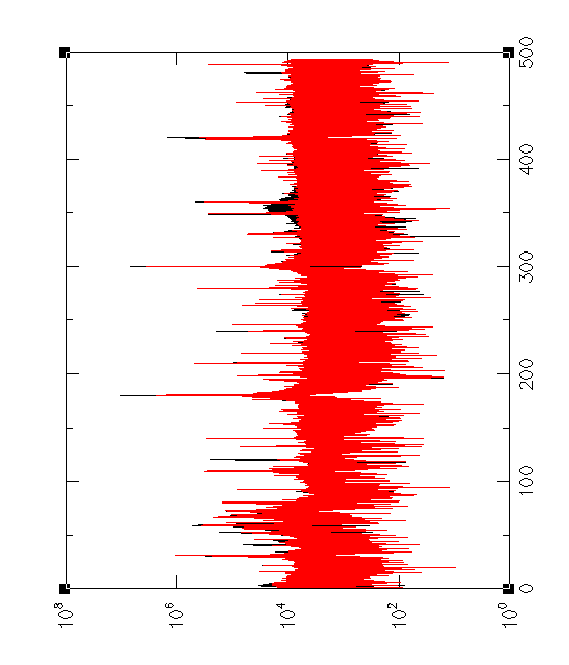
\epsfig{file=Figures/cleaned.eps,angle=270,width=5in}
\caption{ \label{f:cleaned} The spectrum of the IFO\_DMRO channel
before (black) and after `cleaning' based on the three environmental
channels  discussed in the text
using a correlation width of 128 bins (red).}
\end{center}
\end{figure}



The output file  {\tt 40m\_fft/fftclean\_IFO\_128.dat} contains the Fourier
transform  of the corresponding signal `cleaned'
by estimating the transfer functions over a correlation width of
128 bins. 
Figure~\ref{f:cleaned} shows the spectrum of the IFO\_DMRO channel
before and after `cleaning' based on environmental channels 1, 2 and 5.


\clearpage
\subsection{Example: {\tt corr\_init} }



This program calculates the FFTs of the various channels specified in
the configuration file and stores them in binary files in a
subdirectory of the working directory, whose name is determined by the
detector name specified in the configuration file.

\begin{description}
\item{Typical usage:} {\tt corr\_init 40m.config}
\end{description}

\lgrindfile{Includes/corr_init.tex}

\clearpage

\subsection{Example: {\tt env\_corr} }

This program calls {\tt calc\_rho} and {\tt clean\_chan} to determine
environmental correlations. It pops up a graph plotting these 
correlation as well as writing files containing data on the
correlations
and the `cleaned' signal.



\begin{description}
\item{Typical usage:} {\tt env\_corr  40m.config}
\end{description}

\lgrindfile{Includes/env_corr.tex}


\begin{description}
\item{Author:}
Bruce Allen (ballen@dirac.phys.uwm.edu), Wensheng Hua (hua@bondi.phys.uwm.edu)
  and Adrian Ottewill (ottewill@relativity.ucd.ie).
\item{Comments:} None.
\end{description}

\clearpage

% /* GRASP: Copyright 1997,1998,1999  Bruce Allen */
% $Id: man_inspiral.tex,v 1.42 1999/09/29 19:44:41 ballen Exp $
\section{GRASP Routines: Gravitational Radiation from Binary Inspiral}
\label{s:inspiral}
\setcounter{equation}0
One of the principal sources of gravitational radiation which should be
detectable with the first or second generation of interferometric
detectors is {\it binary inspiral}.  This radiation is produced by a
pair of massive and compact orbiting objects, such as neutron stars or
black holes.

The simplest case is when the two objects are describing a circular
orbit about their common center-of-mass, and neither object is spinning
about its own axis.  With these assumptions the system is then
described, at any time, by the masses $m_1$ and $m_2$ of the objects,
and their orbital frequency $\Omega$.  (It is also necessary to
describe the orientation of the orbital plane and the positions of the
masses at a given time; these are details we will sort out later).

For convenience in dealing with dimensional quantities, we introduce
the {\it Solar Mass} $M_\odot$ and the {\it Solar Time} $T_\odot$
defined by
\begin{eqnarray}
M_\odot &=& 1.989 \times 10^{33} \> {\rm grams}\\
\label{e:tsolar}
T_\odot &=& \left( {G \over c^3} \right) M_\odot = 4.925491 \times
10^{-6} \> {\rm sec}.
\end{eqnarray}
GRASP functions typically measure masses in units of $M_\odot$ and
times in units of seconds.
\clearpage

\subsection{Chirp generation routines}
\setcounter{equation}0
The next several subsections document a number of routines 
for generating ``chirps'' from coalescing binaries.  
This package of routines is intended to be versatile, flexible and robust; 
and yet still fairly simple to use.
The implementation we have included in this package is based
on the second post-Newtonian treatment of binary inspiral presented in
\cite{biww} and augmented by the spin-orbit and spin-spin corrections
presented in \cite{willwiseman} and 2.5 post-Newtonian
order corrections in \cite{blanchet:1996}.
The notation we use -- even in the source code  --
closely reflects the notation used in those papers.
In keeping with that notation, these routines calculate
the {\bf orbital phase} and {\bf orbital frequency}. 
The gravitational-wave phase of the dominant quadrupolar radiation
can be obtained by multiplying the orbital phase by two.
The routines can be used to compute a few 
chirp waveforms (say to make transparencies for a seminar),
or for wholesale computations of a bank of matched filters.

All of the chirp generation routines, 
in particular the ubiquitous {\tt make\_filters()}, 
compute what has come to be
known as {\bf  ``restricted'' post-Newtonian chirps}.
This means they include all post-Newtonian corrections
(up to the specified order)
in the phase evolution, but only the dominant quadrupole
amplitude.

The routines are flexible in the sense that they have a number
of {\it run-time} options available for choosing the post-Newtonian
order of the phase calculations, or choosing whether or not
to include spin effects.
We have also isolated those parts of the code where the messy
post-Newtonian coefficients appear;
thus the routines may be
easily modified to include yet higher-order post-Newtonian terms as
they become available.

The post-Newtonian equations for the orbital phase evolution are
notoriously ill-behaved \cite{cutleretal,lincolnwill} as the binary
system nears coalescence.  In this regime the expansion parameters
[namely the relative velocity $v/c$ of the bodies and/or the field
strength $GM_{\rm tot}/(c^2 r_{orbit})$] used in the derivation are
comparable to unity.  In post$^2$-Newtonian calculations higher orders
such as post$^3$-Newtonian terms have been discarded.  Because of this
truncation, quantities that are are positive definite in an exact
calculation (say the energy-loss rate, or the time derivative of the
orbital frequency) often become negative in their post-Newtonian
expansion when the orbital separation becomes small.  When this happens
you are using a post-Newtonian expression in a regime where its
validity is questionable.  This is cause for concern, and it may be
cause for terminating a chirp calculation; but, it need not crash your
code.  A full-scale gravitational-wave search will need to compute
chirps over a broad range of parameters, virtually assuring that any
post-Newtonian chirp generator will be pushed into a region of
parameter space where it doesn't belong.  These routines are designed
to traverse these dangerous regions of parameter space as well as
possible and gently warn the user of the dangers encountered.  The
calling routines may wish to act on the warnings coming from the chirp
generator.  For example a severe warning may prompt the calling routine
to discard a given filter from  a data search, because the second
post-Newtonian calculation of the chirp is so dubious that it can't
give meaningful results.

In the next several sections we detail the use of three routines used
to compute the ``chirp'' of a coalescing binary system.  The first
routine we describe is {\tt phase\_frequency()}.  This is the
underlying routine for the other chirp routines.  Given a set of
parameters ({\it e.g.} the two masses, and the upper and lower cut-off
frequency for the chirp) it returns the orbital phase and orbital
frequency evolution as a function of time.  Next we describe {\tt
chirp\_filter()} which returns two (unnormalized) chirp signals.  This
routine can be used for wholesale production of a bank of templates for
a coalescing binary search.  
%The routine {\tt strain()} returns the
%full second post-Newtonian gravitational wave strain.  This can be used
%for plotting and examining the expected waveform of a given coalescing
%binary, or to add a ``realistic'' signal into detector noise.  The
%strain output contains all the (sub)harmonic structure and its
%amplitude reflects the true astrophysical distance to the source.

\clearpage

\subsection{Function: {\tt phase\_frequency()}}
\label{ss:phase_frequency}
\setcounter{equation}0
{\tt
int phase\_frequency(float m1, float m2, float spin1, float spin2, int n\_phaseterms,
   float *phaseterms, float Initial\_Freq, float Max\_Freq\_Rqst,
   float *Max\_Freq\_Actual, float Sample\_Time, float **phase, float **frequency,
   int *steps\_alloc, int *steps\_filld, int err\_cd\_sprs)
}\\
This function computes the {\bf orbital  phase} 
and {\bf orbital frequency} evolution of
an inspiraling binary. It returns an integer termination code
indicating how and why the chirp calculation terminated.
This routine is the engine that powers the other chirp generation
routines.
The arguments are:
\begin{description}
\item{\tt m1}: Input.  The mass of body-1 in solar masses.
\item{\tt m2}: Input.  The mass of body-2 in solar masses.
\item{\tt spin1}: Input.  The dimensionless spin parameter 
  of body-1. See section on spin effects.
\item{\tt spin2}: Input.  The dimensionless spin parameter 
  of body-2. See section on spin effects.
\item{\tt n\_phaseterms}: Input. Integer describing
 the number of post-Newtonian (pN) approximation terms implemented in
 the phase and frequency calculations. In the present implementation
 this should be set to $5$.
\item{\tt phaseterms}: Input. The array 
  {\tt phase\_terms[0..n\_phaseterms-1]} specifies which pN
  approximation terms will be included in the phase frequency
  calculations.  Setting  {\tt phase\_terms[i]=0.0} nullifys the term.
  Setting  {\tt phase\_terms[i]=1.0} includes the term.  This allows
  for easy run-time nullification of any term in the phase and
  frequency evolution, {\it e.g.} setting {\tt phase\_terms[4]=0.0}
  eliminates the {\it second} post-Newtonian terms from the
  calculation.
\item{\tt Initial\_Freq}: Input.  The starting orbital frequency of the
  chirp in Hz.
\item{\tt Max\_Freq\_Rqst}: Input.  The requested orbital frequency
  where the chirp will stop. However, the actual calculation
  may not proceed all the way to this orbital frequency.  This is 
  discussed at length below.
\item{\tt Max\_Freq\_Actual}: Output. The floating 
  number {\tt *Max\_Freq\_Actual}
  is the orbital frequency in Hz where the chirp actually terminated.
\item{\tt Sample\_Time}: Input.  The time interval between successive samples,
  in seconds.
\item{\tt phase}: Input/Output. The phase ephemeris $\Omega$ in radians
  is stored in the array {\tt *phase[0..steps\_filld-1]}.
  Input in the sense that much of the internal logic of 
  {\tt  phase\_frequency()} depends on how the pointers {\tt *phase}
  (and {\tt *frequency} below) are set.
  If either is set to {\tt NULL} memory allocation will be performed
  inside  {\tt  phase\_frequency()}. If both are not {\tt NULL}
  then it is assumed the calling routine has allocated the memory
  before calling  {\tt  phase\_frequency()}.
\item{\tt frequency}: Input/Output. Similar to {\tt phase} above.
  The frequency ephemeris $f=d\Omega/dt$ is stored in the array 
  {\tt *frequency[0..steps\_filld-1]}.
\item{\tt steps\_alloc}: Input/Output. The integer
  {\tt *steps\_alloc} is the number of floating point entries
  allocated for storing the 
  phase and frequency evolution, {\it i.e.} the length of
  {\tt **phase} and {\tt **frequency}.
  This integer should be set in the calling
  routine if memory is allocated there,
  or it will be set inside {\tt  phase\_frequency()} if memory
  is to be allocated there.
  If both of the pointers {\tt *phase} and {\tt *frequency} are
  not {\tt NULL} then {\tt  phase\_frequency()} understands that
  the calling routine is taking responsibility
  for allocating the memory for the chirp, and the calling routine
  must set {\tt *steps\_alloc} accordingly. 
  In this case {\tt phase\_frequency()} will
  fill up the  arrays  {\tt **phase} and {\tt **frequency} until the memory
  is full ({\it i.e} fill them with {\tt *steps\_alloc} of floats)
  or until the chirp terminates, whichever is less.
\item{\tt steps\_filld}: Output. The integer {\tt *steps\_filld}
  is the integer number of time steps actually computed
  for this evolution. It is less than or equal to {\tt *steps\_alloc}.
\item{\tt clscnc\_time}: Output. The float {\tt *clscnc\_time}
 is the time to coalescence in seconds,
 measured from the instant when the orbital frequency is 
 {\tt Initial\_Freq} given by $t_c$ in Eqs.(\ref{e:frequencyns})
 and (\ref{e:phasens}).
\item{\tt err\_cd\_sprs}: Input. Error code suppression.
 This integer determines
 at what level of disaster encountered in the computation 
 of the chirp the user will be explicitly warned about
 with a printed message.
 Set to {\tt 0}: prints all the termination
 messages. Set to {\tt 4000}: suppresses
 all but a few messages which are  harbingers of complete disaster.
 The termination messages are numbered from 0 to 3999 
 loosely in accordance with their severity
 (the larger numbers corresponding to more severe warnings). 
 Any message with a number less than {\tt err\_cd\_sprs} will not
 be printed.
 A termination code of 0 means the chirp calculation was executed
 as requested.
 A termination code in the 1000's means the chirp was terminated
 early because the post-Newtonian approximation was deemed no longer
 valid.
 A termination code in the 2000's generally indicates some problem with
 memory allocation.
 A termination code in the 3000's generally indicates a serious logic fault.
 Many of these ``3000'' errors result in the termination of the routine.
 If you get an error message number it is easy to find the portion of 
 source code where the fault occurred; just do a character string search
 on the four digit number.
 
\end{description}

This phase and frequency generator has a number of very specialized features 
which will be discussed later. 
However,
before we proceed further, we show a simple example of how  
{\tt phase\_frequency()} can be used.

\begin{description}
\item{Authors:} Alan Wiseman, agw@tapir.caltech.edu and Bruce Allen, ballen@dirac.phys.uwm.edu
\item{Comments:}
This function will need to be extended when results of order 2.5 and 3
post-Newtonian calculations have been reported and published.
\end{description}

\clearpage

\subsection{Example: {\tt phase\_evoltn} program}
\label{ss:phase_evoltn}
\setcounter{equation}0
This example uses {\tt phase\_frequency()} to compute the phase and
frequency evolution for an inspiraling binary and prints the results 
on the screen ({\tt stdout}). 
The other output messages go to {\tt stderr}.
\lgrindfile{Includes/phase_evoltn.tex}
\clearpage

Here is the output from the {\tt phase\_evoltn} example:

{\footnotesize
\begin{verbatim}
GRASP: Message from function phase_frequency() at line number 439 of file "pN_chirp.c".
Frequency evolution no longer monotonic.
Phase evolution terminated at frequency and step: 911.681702    13357
Terminating chirp. Termination code set to:     1201
Returning to calling routine.
$Id: man_inspiral.tex,v 1.42 1999/09/29 19:44:41 ballen Exp $
$Name: RELEASE_1_9_8 $


m1=1.400000  m2=1.400000  Initial_Freq=60.000000
steps_filld=13357  steps_alloc=16384  Max_Freq_Actual=911.681702
time_in_band=1.353408 clscnc_time=1.353573
Termination code: 1201

0       0.000000        0.000000        60.000000
1       0.000101        0.038204        60.001675
2       0.000203        0.076369        60.003353
3       0.000304        0.114627        60.005020
4       0.000405        0.152820        60.006695
5       0.000507        0.191071        60.008366
6       0.000608        0.229173        60.010052

 ...      ...             ...              ...

13349   1.352699        797.669800      720.294189
13350   1.352800        798.134949      741.157715
13351   1.352901        798.614136      764.565796
13352   1.353003        799.109192      791.015686
13353   1.353104        799.622192      821.015320
13354   1.353205        800.155457      854.720337
13355   1.353307        800.710999      890.133667
13356   1.353408        801.286499      911.681702
\end{verbatim}
}

The first seven lines of output come directly from {\tt phase\_frequency()},
and are printed to {\tt stderr}.
These give a warning message telling why the chirp calculation was terminated;
it no longer had monotonically increasing frequency.
It also tells where the chirp was terminated;
after computing {\tt 13357} points it has reached a frequency of {\tt 907}Hz.
The termination code ({\tt 1201}) is also printed. Knowing the termination
code makes it easy to find the segment of source code that produced the
termination; just do a search for the character string ``{\tt 1201}'' 
and you will find the line of code where the termination code was set.
Setting {\tt err\_cd\_sprs} greater than {\tt 1201} would suppress
the printing of this warning message and all messages with
a termination code less than {\tt 1201}.  
However, even without the
printed message the calling routine  can
determine the value of the termination code; it is returned
by {\tt phase\_frequency()}.

The rest of the output comes from the
{\tt phase\_evoltn} program. The quantity 
{\tt time\_in\_band}$=(${\tt steps\_filld}$-1)\times${\tt Sample\_Time}
is the length (in seconds) of the computed chirp.
The quantity {\tt clscnc\_time} is the value of
$t_c$ that enters Eqs.(\ref{e:frequencyns}) below.
The four column output from left to right is the integer
index of the data points, time stamp of each point in seconds (starting
arbitrarily from zero), the orbital phase in radians (starting arbitrarily
from zero), and the orbital frequency (starting from
the initial frequency of {\tt 60}Hz).

To summarize:
It takes about {\tt 1.35} seconds
for two {\tt 1.4}$M_\odot$ objects to spiral in from an orbital
frequency of {\tt60}Hz to an orbital frequency of {\tt 911}Hz.
The chirp calculation was terminated at {\tt 911}Hz -- instead of the
requested {\tt 2000}Hz -- 
because the post-Newtonian expression used to compute
the chirp is clearly out of its region of validity:
the frequency is no longer increasing.
Examining the last few data points shows that the frequency was
rising quickly -- as expected -- until the last two data points.
During this inspiral the orbital system went through
{\tt 811.09}$/(2 \pi)\approx ${\tt 127.53} revolutions.
The two integer numbers {\tt steps\_filld} and {\tt steps\_alloc}
are the number of actual data points computed and the number
of floating point memory slots allocated, respectively.
(Memory is allocated in blocks of 4096 floats at a time. Thus
{\tt steps\_alloc} will generally exceed  {\tt steps\_filld}.)
The  values of the
phase and frequency at every $1/${\tt Sample\_Time}$=1.10333\times10^{-4}$
seconds starting from when the binary had an orbital frequency of
{\tt 60}Hz until it neared ``coalescence'' at {\tt 911}Hz have
been calculated.
\clearpage

\subsection{Detailed explanation of {\tt phase\_frequency()} routine}
\setcounter{equation}0
The {\tt phase\_frequency()} routine starts with inputs describing
the physical properties of the system (the masses)
and an initial frequency from which to start the evolution.
We then compute the orbital frequency evolution [in cycles/second] directly
from the formula given in \cite{biww}
\begin{eqnarray}
\label{e:frequencyns}
f(t)&=& {M_\odot \over 16 \pi  T_\odot m_{\rm tot}} 
\biggl\{ \Theta^{-3/8} +\left({743\over 2688}
 + {11\over 32}\eta \right) \Theta^{-5/8} - {3\pi \over 10} \Theta^{-3/4} \nonumber \\
&&\qquad\qquad\qquad+ \left( {1855099\over 14450688}
+ {56975\over 258048} \eta + {371\over 2048} \eta^2 \right) \Theta^{-7/8}
\biggr\} \;,
\end{eqnarray}
%label{e:frequencyns}
where $m_{\rm tot}$ is the total mass of the binary.  The time integral
of this equation gives the orbital evolution in cycles.  Multiplying by
$2 \pi$ yields the orbital phase in radians
\begin{eqnarray}
\label{e:phasens}
\phi (t) &=&\phi_c -{1\over\eta} \biggl\{ \Theta^{5/8} +\left({3715\over 8064}
 + {55\over 96}\eta \right) \Theta^{3/8} 
 - {3\pi \over 4} \Theta^{1/4}  \nonumber \\
&&\qquad\qquad\quad+\left({9275495\over 14450688}+{284875\over 258048}
\eta\ +{1855\over 2048} \eta^2 \right) \Theta^{1/8} \biggr\}\;.
\end{eqnarray}
%label{e:phasens}
Here $\Theta$ is a dimensionless time variable
\begin{equation}
\label{e:theta}
\Theta={\eta M_\odot \over 5 T_\odot m_{\rm tot}} (t_c-t) \; ,
\end{equation}
%label{e:theta} $\mu$ is the reduced mass,
$\eta = \mu/m_{\rm tot}$, and $t_c$ is the time of coalescence of the
two point masses. 
Similarly the constant $\phi_c$ is the 
phase at coalescence, which is arbitrarily set 
in {\tt phase\_frequency()} so that $\phi=0$
at the initial time.
[See the detailed discussion of the phase conventions below.]
Also notice that the mass quantities only appear as ratios with the 
solar Mass $M_\odot$, and the time only appears as a ratio with
the quantity $T_\odot = 4.925491\times 10^{-6}\> \rm sec$ in 
Eq.(\ref{e:tsolar}). 

These formulations of the post-Newtonian equations for the phase and
frequency are simple to implement:  each pass through the loop
increments the time by the sample time ({\tt Sample\_Time} in the
example) and computes the phase and frequency using Eqs.
(\ref{e:frequencyns}) and (\ref{e:phasens}).  However, there is an
alternative formulation.  In deriving these  equations the ``natural''
equation that arises is of the form $\dot f= F(f)$. [See {\it e.g.}
\cite{bdiww} Eq.(3).]  This in turn can be integrated to give an
equation of the form $t_c-t = T(f)$.  In our formulation this equation
has been inverted -- throwing away higher-order post-Newtonian terms as
you go -- to give Eq.(\ref{e:frequencyns}).  However the  equation in
the form  $t_c-t = T(f)$ can also be implemented directly.  In this
type of formulation one would again increment the time, but then use a
root-finding routine to find the frequency at each time step. Our
chosen method has the advantage of avoiding a time-consuming
root-finder at each time step; however the alternative
%[$t_c-t =T(f)$]
formulation has undergone fewer damaging post-Newtonian
transformations, and may therefore be more accurate.

In our formulation we only need to call a root-finding routine at the
start of the chirp to find the value of $t_c-t$ when the system is at
the initial frequency.  In order to insure that we find the correct
root for the starting time we begin a search at a time when the leading
order prediction of the frequency is well below the desired starting
frequency.  We step forward in time until we bracket the root; we then
call the {\it Numerical Recipes} root-finder {\tt rtbis()} to compute
the root precisely.  This is depicted in the lower right corner of
figure \ref{f:pNcutoff} where we show the value of the ``time''
coordinate $X$ that corresponds to an initial frequency of $60$Hz.
This method is virtually assured of finding the {\it correct} root in
that it will find the first solution as we proceed from right to left
in figure  \ref{f:pNcutoff}.  The primary problem in finding this root
is that there may actually be no meaningful start-time for the
specified chirp.  For example, if you you were to specify a chirp with
two $1.4M_\odot$ objects with an initial frequency of 1000Hz, you can
see from the figure that there is no value of $X$ ({\it i.e.} $t_c-t$)
that corresponds to this frequency.  In this case {\tt
phase\_frequency()} will search from right to left for the start time.
It will notice that it is passing over the peak in the graph and out of
the regime of post-Newtonian viability.  It will then terminate the
search and notify the caller that there is no solution for the
requested chirp.

The behavior of the frequency equation is shown in figure
\ref{f:pNcutoff}.  As time increases the frequency rises to a maximum
and then begins to decrease dramatically.  Notice that the maximum
occurs when the dimensionless time parameter $\Theta={\eta(t_c-t) \over
5 T_\odot m_{\rm tot} } = X^8$ is approximately  unity; this feature is
only weakly dependent on the mass ratio.  The fact that $\Theta \approx
1$ means the post-Newtonian corrections in Eq.(\ref{e:frequencyns}) are
comparable to the leading order term.  Therefore, this peak is a
natural place to terminate the post-Newtonian chirp approximation.  In
the example the code terminated the chirp for precisely this reason.
[See the warning message.]

Although it is not shown in the figure the behavior of $f$ as $X$ nears
zero is very abrupt; the function goes sharply negative and then turns
around and diverges to $+\infty$ as $X\rightarrow 0$ ({\it i.e.}
$t\rightarrow t_c$).  This abrupt behavior will happen on a time scale
of order $T_\odot$ (a few microseconds).  Typical sample times are
likely to be on the order of a tenth of a millisecond, and therefore
the iterative loop may step right over this maximum-minimum-divergence
behavior of the frequency function altogether.  Don't worry.  The
routine {\tt phase\_frequency()} handles this case gracefully.  The
routine will stop the chirp calculation and warn the caller if the time
stepper goes beyond the coalescence time.  It will also stop the chirp
calculation if it senses that the time has stepped over the dip in
frequency and is on the strongly divergent part of the frequency curve
near the $X=0$ axis.

\begin{figure}[h]
\begin{center}
\epsfig{file=Figures/fig_pNcutoff.ps,angle=-90,width=6in}
\caption{ \label{f:pNcutoff}
Orbital frequency as a function of the ``time'' coordinate
$X=\biggl ( {\eta (t_c-t) M_\odot \over 5 T_\odot m_{\rm tot} } \biggr )^{1/8}$. }
\end{center}
\end{figure}

\clearpage

\subsection{Function: {\tt chirp\_filters()}}
\label{ss:chirp_filters}
\setcounter{equation}0
{\tt int chirp\_filters(float m1, float m2, float spin1, float spin2, int n\_phaseterms,
   float *phaseterms, float Initial\_Freq, float Max\_Freq\_Rqst, float
   *Max\_Freq\_Actual, float Sample\_Time, float **ptrptrCos, float
   **ptrptrSin, int *steps\_alloc, int *steps\_filld, int
   err\_cd\_sprs)
}\\
This function is a basic stripped-down chirp generator.  It computes
two -- nearly orthogonal --  chirp waveforms for an inspiraling
binary.  The two chirps differ in phase by $\pi/2$ radians.  The chirp
values are given by Eqs.(\ref{e:chirpcos}) and (\ref{e:chirpsin}).
Just as the phase and frequency calculator {\tt phase\_frequency()}
returns an integer number which describes how the chirp calculation
was terminated, this routine does also.

The arguments are:
\begin{description}
\item{\tt m1}: Input.  The mass of body-1 in solar masses.
\item{\tt m2}: Input.  The mass of body-2 in solar masses.
\item{\tt spin1}: Input.  The dimensionless spin parameter 
  of body-1. See section on spin effects.
\item{\tt spin2}: Input.  The dimensionless spin parameter 
  of body-2. See section on spin effects.
\item{\tt n\_phaseterms}: Input. Integer describing 
 the number of terms implemented in the phase and frequency 
 calculations. In the present implementation this should be 
 set to $5$.
\item{\tt phaseterms}: Input. The array 
  {\tt phase\_terms[0..n\_phaseterms-1]} describes which 
  terms will be included in the phase frequency calculations.
  Setting  {\tt phase\_terms[i]=0} nullifys the term.
  Setting  {\tt phase\_terms[i]=1} includes the term.
  This allows for easy run-time nullification of any term in the 
  phase and frequency evolution, {\it e.g.} setting 
  {\tt phase\_terms[4]=0} eliminates the second post-Newtonian
  terms from the calculation.
\item{\tt Initial\_Freq}: Input.  The starting orbital frequency of the
  chirp in Hz.
\item{\tt Max\_Freq\_Rqst}: Input.  The requested orbital frequency
  where the chirp will stop. However, the actual calculation
  may not proceed all the way to this orbital frequency.
\item{\tt Max\_Freq\_Actual}: Output. The floating 
  number {\tt *Max\_Freq\_Actual}
  is the orbital frequency in Hz where the chirp actually terminated.
\item{\tt Sample\_Time}: Input.  The time interval between points
  in seconds.
\item{\tt ptrptrCos}: Input/Output. 
  The chirp corresponding to Eq.(\ref{e:chirpcos}) is stored in
  \linebreak[4] {\tt *ptrptrCos[0..steps\_filld-1]}.  Input in the
  sense that much of the internal logic of {\tt  chirp\_filters()}
  depends on how the pointers {\tt *ptrptrCos} (and {\tt *ptrptrSin}
  below) are set.  If either is set to {\tt NULL} memory allocation
  will be performed inside  {\tt  chirp\_filters()}. If both are not
  {\tt NULL} then it is assumed the calling routine has allocated the
  memory before calling  {\tt  chirp\_filters()}.
\item{\tt ptrptrSin}: Input/Output. Similar to {\tt ptrptrCos} above.
  The chirp corresponding to Eq.(\ref{e:chirpsin}) is stored in
  {\tt *ptrptrSin[0..steps\_filld-1]}.
\item{\tt steps\_alloc}: Input/Output. The integer
  {\tt *steps\_alloc} is the number of floating point entries allocated
  for storing the two chirps, {\it i.e.} the number of valid
  subscripts in the arrays {\tt **ptrptrCos} and {\tt **ptrptrSin}.
  This integer should be set in the calling routine if memory is
  allocated there, or it will be set inside {\tt  chirp\_filters()} if
  memory is to be allocated there.  If both of the pointers {\tt
  *ptrptrCos} and {\tt *ptrptrSin} are not {\tt NULL} then {\tt
  chirp\_filters()} understands that the calling routine is taking
  responsibility for allocating the memory for the chirp, and the
  calling routine must set {\tt *steps\_alloc} accordingly.  In this
  case {\tt chirp\_filters()} will fill up the arrays  {\tt
  **ptrptrCos} and {\tt **ptrptrSin} until the memory is full ({\it
  i.e} fill them with {\tt *steps\_alloc} of floats) or until the chirp
  terminates, whichever is less.
\item{\tt steps\_filld}: Output. The integer {\tt *steps\_filld}
  is the number of time steps (sample values) actually computed
  for this evolution. It is less than or equal to {\tt *steps\_alloc}.
\item{\tt clscnc\_time}: Output. The float {\tt *clscnc\_time}
 is the time to coalescence in seconds,
 measured from the instant when the orbital frequency is 
 {\tt Initial\_Freq} given by $t_c$ in Eqs.(\ref{e:frequencyns})
 and (\ref{e:phasens}).
\item{\tt err\_cd\_sprs}: Input. 
 Error code suppression.  This integer specifies the level of disaster
 encountered in the computation of the chirp for which the user will be
 explicitly warned with a printed message.  Set to {\tt 0}: prints
 all the termination messages. Set to {\tt 4000}: suppresses
 all but a few messages which are  harbingers of true disaster.  The
 termination messages are numbered from 0 to 3999 loosely in accordance
 with their severity (the larger numbers corresponding to more severe
 warnings).  Any message with a number less than {\tt err\_cd\_sprs}
 will not be printed.  A termination code of 0 means the chirp
 calculation was executed as requested.  A termination code in the
 1000's means the chirp was terminated early because the post-Newtonian
 approximation was deemed no longer valid.  A termination code in the
 2000's generally indicates some problem with memory allocation.  A
 termination code in the 3000's generally indicates a serious logic
 fault.  Many of these ``3000'' errors result in the termination of the
 program.  If you get an error message number it is easy to find the
 portion of source code where the fault occurred; just do a character
 string search on the four digit number.
\end{description}
\begin{description}
\item{Authors:} Alan Wiseman, agw@tapir.caltech.edu and Bruce Allen, ballen@dirac.phys.uwm.edu
\item{Comments:}
None.
\end{description}
\clearpage

\subsection{Detailed explanation of {\tt chirp\_filters()} routine}
\setcounter{equation}0
The routine {\tt chirp\_filters()} calls {\tt phase\_frequency()} to find out the
how the orbital phase and frequency evolve in accordance with the 
input parameters. 
It then makes a single pass
through that phase and frequency ephemeris, computing the chirps as it goes,
and storing the information in the space already allocated
for the phase and frequency.
Most of the fault checking and computations are
done in the {\tt phase\_frequency()} routine,
and all the errors messages and warnings come from there.

The routine {\tt chirp\_filters()} computes
\begin{equation}
\label{e:chirpcos}
h_c(t) = 2 \biggl ({\mu \over M_\odot} \biggr )
\biggl [ { 2 \pi T_\odot m_{\rm tot} f(t) \over M_\odot  } \biggr ]^{2/3} 
\cos 2 \phi (t)
\end{equation}
and the other orbital-phase chirp which is $\pi/2$ out of phase with $h_c (t)$
\begin{equation}
\label{e:chirpsin}
h_s(t) = 2 \biggr ( {\mu \over M_\odot} \biggr )
\biggl [ { 2 \pi T_\odot m_{\rm tot} f(t) \over M_\odot  } \biggr ]
^{2/3} \sin 2 \phi (t) \; ,
\end{equation}
with all the leading numerical factors we display.

If the so called ``restricted'' post$^2$-Newtonian polarizations 
[leading order in the amplitude, but post$^2$-Newtonian phase corrections]
are desired, they can be easily  assembled from $h_c$ and $h_s$.
The ``$+$'' (plus) polarization is given by
\begin{equation}
h_{+}(t) = - { T_\odot c \over D} (1+\cos^2 i ) h_c(t) \; ,
\end{equation}
and the ``$\times$" (cross) polarization is given by
\begin{equation}
h_\times (t) = -2  { T_\odot c \over D} ( \cos i ) \; h_s(t) \; .
\end{equation}
Here $D$ is the (luminosity) distance to the source in centimeters,
c is the speed of light in centimeters/second,
and $i$ is the inclination angle (radians) of the of the angular momentum
axis of the source relative to the line-of-sight.  
See Will and Wiseman \cite{willwiseman} figure 7 for the precise definition
of the inclination angle.

The restricted post$^2$-Newtonian strain amplitude
impinging on the detector can also be calculated from the
output of {\tt chirp\_filters()} by
\begin{equation}
h(t) = F_+ h_+(t) + F_\times h_{\times}(t) \; ,
\end{equation}
where $F_+$ and $F_\times$ are the detector beam-pattern functions.

In the remainder of this section we will clarify some technical issues 
involving the orbital phase. 
First, in computing  $\phi (t)$ in {\tt phase\_frequency()} we have arbitrarily
set the constant $\phi_c$ in Eq.(\ref{e:phasens})
such that $\phi=0$ at the beginning of the chirp.
The astrophysical convention for defining the 
orbital phase angle $\phi$ given in \cite{willwiseman}
measures $\phi$ in the plane of the orbit from the ascending node.
[The ascending node of the orbit is where body-1 passes through the plane
of the sky going away from the observer.]
Choosing $\phi_c$ in this way we have assumed that
body-1 is passing through the ascending node of the orbit
at the instant we start our chirp.
Detailed information about the overall phase 
is not needed for many purposes ({\it i.e.} matched filters),
therefore our choice is of little consequence.
If this information  needs to be included for some application,
{\tt chirp\_filters()} can be modified to do so;
thus one can leave the computational engine {\tt phase\_frequency()} 
untouched.

The second issue involving the phase is a bit more delicate. 
We have used the true orbital phase $\phi(t)$ to
compute oscillatory part of the chirp in 
Eqs.(\ref{e:chirpcos}) and (\ref{e:chirpsin}). 
But should we use the logarithmically  modulated phase variable
\begin{equation}
\label{e:psidef}
\psi (t) = \phi - { 4 G m_{\rm tot} \pi f(t) \over c^3} \ln[f(t)/f_o] 
\end{equation}
%label{e:psidef}
in our computation of the chirp?
After all, the true  phase of the gravitational-wave signal
impinging on the detector is $2\psi$.
Let us examine the effect on our signal
replacing $\sin 2 \phi$ in Eq.(\ref{e:chirpsin})
with the logarithmically corrected  $\sin 2 \psi$
\begin{eqnarray}
\label{e:psiphi}
\sin 2 \psi &=& \sin \biggl ( 2\phi-{8\pi m_{\rm tot} f G \over c^3} \ln(f(t)/f_o) \biggr)
\nonumber \\
&& =  \sin 2 \phi  \cos \biggl ( {8\pi m_{\rm tot} f G \over c^3}  \ln(f(t)/f_o) \biggr )
   -  \cos 2 \phi  \sin \biggl ( {8\pi m_{\rm tot} f G \over c^3}  \ln(f(t)/f_o) \biggr )
\nonumber \\
&& \approx \biggl ( 1 +O(1/c^6) \biggr ) \sin 2 \phi
         - \biggl ( {8\pi m_{\rm tot} f G \over c^3} \ln(f(t)/f_o) \biggr )\cos 2\phi \; .
\end{eqnarray}
The $O[1/c^6]$ is a post$^3$-Newtonian term and can be neglected in
the present  post$^2$-Newtonian analysis.
However the coefficient of the $\cos 2 \phi$ is a post$^{3/2}$-Newtonian
order correction to the waveform, and must be included in
any full post$^2$-Newtonian analysis. 
This logarithmic term is included in the waveform calculation 
in the {\tt strain()} routine.
However, the last line of Eq.(\ref{e:psiphi}) also shows that the logarithmic
phase correction
can be considered a post$^{3/2}$-Newtonian correction to the amplitude.
In our present restricted post-Newtonian chirp calculation we
neglect these higher order amplitude corrections,
so we are justified in neglecting the logarithmic correction to  the phase.

The advantage of neglecting the logarithm is that it speeds up the 
calculation of the chirps: we don't have to compute a logarithm at
each time step. However, this may be at expense of accurately tracking
the signal phase of a strongly relativistic source. After all much research has
gone into computing the gravitational wave phase from these
sources and we shouldn't willy-nilly discard these phase corrections.
Is it difficult to modify our code to include this term?
Not at all.  
In fact, the inclusion of the logarithmic correction
to the gravitational wave phase would not affect
{\tt phase\_frequency()}, at all.
The fact that this logarithmic propagation 
effect only enters the {\tt chirp\_filters()} routine
and not the {\tt phase\_frequency()} routine
may seem like a computational quirk, but this actually has
a physical origin:
The routine {\tt phase\_frequency()} computes the local orbital
phase of the binary;
whereas, the physical origin of the logarithmic term is a {\it propagation}
effect and has nothing to do with the orbital phase,

This is not say that no log terms will ever be needed in 
{\tt phase\_frequency()}. 
Note that at post$^4$-Newtonian
order there are log terms which do affect the local instantaneous
orbital motion of the binary,
so if {\tt phase\_frequency()} is ever modified to 
incorporate that order, then log terms will appear there also.

Another issue involving the log term in the phase is the presence of
the ``arbitrary'' scale factor $f_o$
entering the definition of $\psi (t)$ in Eq.(\ref{e:psidef}).
%It gives the impression that the physical gravitational wave
%signal from a distant binary source depends on some arbitrary 
%constant chosen by the person writing the software to analyze the signal.
%In spite of the appearance this is not the case.
The net effect of adjusting this constant is to change the value of
another arbitrary constant in our phase and frequency equations;
it shifts the value of $t_c$  in Eq.(\ref{e:theta}).
%In other words, changing the value of $f_o$ has no 
%more effect on the signal than does changing the clocks in the lab to 
%daylight savings time.
In order to to facilitate swift computation,
we choose $f_o$ to be the minimum frequency of the 
requested chirp.
This insures that the ratio in the logarithm is of order unity during
the chirp computation.
 \clearpage

\subsection{Example: {\tt filters} program}
\setcounter{equation}0
\label{ss:filters}
This example uses {\tt chirp\_filters()}
to generate two chirps $\pi/2$ out of phase with each other.
It also  demonstrates a different memory allocation option than 
the {\tt phase\_evoln} example program.
\lgrindfile{Includes/filters.tex}

Notice that we only allocated enough memory for 10000 points,
and we know from the output from the  previous example that this chirp 
takes {\tt 13515} points. Therefore running this example results
in following error message printed to {\tt stderr}:

\begin{verbatim}
GRASP:phase_frequency():Allocated memory is filled up before
reaching the maximum frequency requested for this chirp.
Orbital Frequency Reached(Hz): 98.867607, Number of points: 10000
Terminating chirp. Termination code set to:     2001
Returning to calling routine.
\end{verbatim}

However, even though the routine ran out of memory it still computed
the first {\tt 10000} points of the chirp and returned them in the
arrays {\tt *ptrptrCos[0..steps\_alloc-1]}  and \linebreak[4] {\tt
*ptrptrSin[0..steps\_alloc-1]}.


\begin{figure}
\begin{center}
\epsfig{file=Figures/chirp.ps,angle=-90,width=5in}
\index{colorpage}
\caption{ \label{f:chirp}
The zero-phase chirp waveform from a $2 \times 1.4 M_\odot$ binary system,
starting at an orbital frequency of 60 Hz.  The top graph shows the frequency
of the dominant quadrupole radiation as a function of time, and the middle graph
shows the waveform.  The bottom graph shows a 40-msec stretch near the final
inspiral/plunge.}
\end{center}
\end{figure}

\clearpage

\subsection{Practical Suggestion for Setting Up a Large Bank of Filters:}
\label{ss:practical}
\setcounter{equation}0

We have carefully explained (how to avoid) 
a number of the pitfalls in computing post-Newtonian chirps.
Before using the chirp generators to
spit out hundreds or thousands of chirps needed for 
a bank of filters and farming out the computations out to dozens
of parallel processors in a massive coalescing binary search,
we strongly suggest that you edit the examples already given
and check the routine against
the {\bf three} extreme cases you will encounter in your search. 
\begin{enumerate}
\item
Try the example with both masses set to the minimum mass in your
proposed search, {\it i.e.} compute the phase and frequency evolution
and the chirps for the template in the upper right hand corner in
figure \ref{f:taurange}.  This is the template of longest duration. If
you are going to have a memory allocation problem you will have it with
this template.  Also, knowing the duration of the longest template
in your search will help you decide the length of the segments of
data which you filter.  In general, you want the length of these data
segments to be at least several times longer than the longest chirp.
See Section~\ref{ss:dirty} for further details.
\item
Try the chirp generator with both masses set to the maximum mass in
your search, {\it i.e.} compute the phase and frequency evolution
of the template in the lower left corner of figure \ref{f:taurange}.
This is the shortest duration template and the one least likely to make
it to the upper cut off frequency before going out of the region of
post-Newtonian viability.  This case will be the most demanding test
of the ``chirp-termination'' logic in {\tt phase\_frequency()}.  It is
also possible in the case of extremely large masses that there really
is no chirp at all in the frequency regime requested.  For example a
binary composed of two 100$M_\odot$ object will coalesce long before
it reaches the initial chirp frequency of the 60Hz we are using as our
a lower cutoff frequency in our example. Don't worry. The routine {\tt
phase\_frequency()} will warn you that the root finder was unable to
find a viable solution for the initial time.  You may have to adjust
the search range accordingly.
\item
Try the chirp generator with one mass at the minimum
allowed value and the other mass at the maximum allowed value,
{\it i.e.} compute the phase and frequency evolution for the template
in the upper left corner of figure \ref{f:taurange}.
This is the template which is
most dominated by post-Newtonian terms in the evolution.
\end{enumerate}
If the routine gives satisfactory results for these three 
cases, it should work for all the cases shown 
in figure \ref{f:taurange}; you are now ready for wholesale production.
\clearpage

\subsection{Additional contributions to the phase and frequency of the chirp}
\label{ss:additional}
\setcounter{equation}0

In recent years additional relativistic corrections to the
binary inspiral chirp formula have been calculated. 
These have now been
included in GRASP, and are available to users generating template banks.  
The changes have been implemented in existing GRASP routines, and
using  them requires minimal modification of your code.
Furthermore, {\it if you have written GRASP code that uses
only second post Newtonian chirps -- and you want to
keep it that way  -- you don't need to do anything: all the
modifications are compatible with previous GRASP releases.}

When the original code for the GRASP chirp generator was
written, only the second post-Newtonian relativistic
corrections to the phase  and frequency evolution were
available.  These are depicted in Eqs. (\ref{e:frequencyns})
and (\ref{e:phasens}), and implemented in the {\tt
phase\_frequency()}  routine.  The routine used for
generating template banks, {\tt make\_filters()}, uses these
formulae by calling {\tt phase\_frequency()}.  In the next
two subsubsections we discuss extensions of these formulae
and routines to include the contributions to the phase and
frequency produced by the spins of the objects (spin-orbit
coupling, and spin-spin coupling) and also the contribution
from the 2.5 post-Newtonian order corrections.
In future GRASP releases  we hope to include contributions
to the phase and frequency produced by the quadrupole moment
of the bodies and higher-order post-Newtonian effects.

\subsubsection{Spin Effects}
\label{sss:spin}
\setcounter{equation}0
In the simple case where the spin vectors of the bodies
are aligned (or antialigned) with the orbital angular momentum
axis, the GRASP chirp-generating
functions have the built-in capability of computing the leading order
{\bf spin-orbit} and {\bf spin-spin} corrections to the
inspiral chirp.
To use this feature no modification of the chirp-generating routines 
[{\tt phase\_frequency()} or {\tt chirp\_filters()}] is necessary;
simply pass nonzero values of the spin parameters to the functions.
This can easily be done by editing the example programs 
{\tt phase\_evoltn.c} and/or {\tt filters.c} to
pass nonzero values of the variables {\tt spin1} and {\tt spin2}.
[See below for definitions and allowed ranges of {\tt spin1} and {\tt spin2}.]

When spinning bodies are involved, the full gravitational
waveform can be quite complicated; the orbital plane 
and the spin vectors of the individual bodies can
precess.  The precession causes a modulation of the signal.
However, this GRASP routines only implements the the special case 
when the spins are assumed to be aligned (or antialigned) with the
orbital angular momentum axis.
In this case there is no precession and, therefore, no modulation
of the amplitude of the signal.
Also in this case,
the spin-corrections to the orbital frequency and phase 
are given by simple modifications to the nonspin phase and frequency
Eqs. (\ref{e:frequencyns}) and (\ref{e:phasens}).
The necessary terms can be found in Eq.(F22) in Appendix F of \cite{willwiseman},
and are given by
\begin{eqnarray}
\label{e:frequencyspin}
f(t)&=& {M_\odot \over 16 \pi  T_\odot m_{\rm tot}} 
\biggl\{ \Theta^{-3/8} + \; {\rm ...} \;\
+\left({113\over160} [\chi_s + (\delta m /m) \chi_a] -{19\over40}\eta \chi_s \right)
\Theta^{-3/4} \nonumber \\
&&\qquad\qquad\qquad
-\left( {237\over 512} \eta [(\chi_s)^2 -(\chi_a)^2] \right) \Theta^{-7/8}
 \;\biggr\} \;,
\end{eqnarray}
%label{e:frequencyns}
and
\begin{eqnarray}
\label{e:phasespin}
\phi (t) &=&\phi_c -{1\over\eta} \biggl\{ \Theta^{5/8} + \; {\rm ...} \; 
+\left({113\over64} [\chi_s + (\delta m /m) \chi_a] -{19\over16}\eta \chi_s \right)
\Theta^{1/4} \nonumber \\
&&\qquad\qquad\quad
-\left( {1185\over 512} \eta [(\chi_s)^2 -(\chi_a)^2] \right) \Theta^{1/8}
 \; \biggr\}\;.
\end{eqnarray}
%label{e:phasens}
Here $\Theta$ is the dimensionless time variable given by Eq. (\ref{e:theta}).
The ellipses represent the nonspin (post)$^n$-Newtonian terms already given
in Eqs. (\ref{e:frequencyns}) and (\ref{e:phasens}).
The quantities $\chi_s$ and $\chi_a$ are dimensionless
quantities related to the
angular momentum of the bodies by
\begin{eqnarray}
\label{e:chi_defn}
\chi_s={1\over 2}\left({ S_1 \over m_1^2}+{ S_2 \over m_2^2} \right) \; , \\
\chi_a={1\over 2}\left({ S_1 \over m_1^2}-{ S_2 \over m_2^2} \right) \; ,
\end{eqnarray}
where $S_{1(2)}$ is the signed magnitude of the angular momentum vector of each body
expressed in geometrized units (cm$^2$), and $m_i$ is the
mass in geometrized units (cm).
[Below we show how to covert from geometrized units to cgs units.]
The sign is positive (negative) for spins aligned (antialigned) with the 
the angular momentum axis.
By comparing the nonspin phase and frequency  evolution 
in Eqs. (\ref{e:frequencyns}) and (\ref{e:phasens})
with the spin corrections in Eqs. (\ref{e:frequencyspin}) and (\ref{e:phasespin}),
we see that the spin-orbit corrections (terms linear 
in $\chi_s$ and $\chi_a$) simply modify the (post)$^{3/2}$-Newtonian
contributions
and the spin-spin corrections (term quadratic in $\chi_s$ and $\chi_a$)  
modify the (post)$^{2}$-Newtonian contributions.

Specifically, the spin quantities passed to the chirp generation routines 
are the signed, dimensionless (Kerr-like) parameters of each body
\begin{eqnarray}
{\tt spin1} = \pm { |{\bf S_1} | \over m_1^2 } \; ,  \\
\label{e:spin_defn}
{\tt spin2} = \pm { |{\bf S_2} | \over m_2^2 } \; ,
\end{eqnarray}
where the $+(-)$ sign is chosen if the spin is aligned (antialigned)
with the orbital angular momentum axis.
[Note: only in Eqs.(\ref{e:chi_defn})-(\ref{e:spin_defn})
is mass expressed in geometrized units.]

Some calculations
({\it e.g.} those requiring a precise definition of the
orbital phase) are sensitive to the index assigned to
the bodies.
The GRASP convention is that $m_1$ is the smaller of
the two masses;
therefore {\tt spin1} should be the spin assigned to 
the smaller of the two masses.

How are the dimensionless spin parameters {\tt spin1(2)}
and the geometrized angular momentum $\bf S_i$
related to angular momentum of the bodies in cgs units?
Let $L_i$ denote the spin angular momentum 
of the i-th body in cgs units
({\it i.e.} gram cm$^2$/sec).
Then $L_i$ is related to $S_i$ by
\begin{eqnarray}
S_i \; [{\rm in\;geometrized\;units}, i.e. \; {\tt cm^2} ] &=& \;
\left({G \over c^3 }\right)  
L_i\;({\rm in \; gram\;cm^2/sec})  \;  \nonumber \\
&=& 2.477 \times 10^{-39}({\rm sec /gram}) 
\; L_i\;({\rm in \; gram\;cm^2/sec})  \; .
\end{eqnarray}
The conversion of angular momentum in cgs units
to the {\bf dimensionless} variable {\tt spin1(2)} 
(the variable actually sent to the routine)
is
\begin{equation}
\label{e:cgstogeom}
{\tt spini} = \left( {c \over G m_{i}^2 } \right)  L_i
= \left( {c \over G m_\odot^2 } \right) 
\left(  {M_\odot \over m_i} \right)^2 L_i
= 1.136 \times 10^{-49}  ({\rm sec / (gram \; cm^2) })
\left(  {M_\odot \over m_i} \right)^2 L_i
\end{equation}
where $L_i$ is the magnitude of the spin angular momentum of the i-th body 
in standard cgs units ({\it i.e.} gram cm$^2$/sec),  
and $m_i$ is the mass in grams.

What is the allowable range for the spin parameters {\tt spin1} and {\tt spin2}?
For Kerr black holes, we know $|{\tt spin1(2)}| = (|{\bf S_{1(2)}} | / m_{1(2)}^2 ) \leq 1$.
For spinning neutron stars, stability studies
(based on relativistic numerical hydrodynamic simulations)
show that the spin parameter must satisfy
$|{\tt spin1}({\tt 2})| = (|{\bf S_{1(2)}} | / m_{1(2)}^2 )
\mathrel{\raise.3ex\hbox{ $<$ } \mkern-14mu \lower0.6ex\hbox{$\sim$ } } 0.6$.
These limits can serve as a hard upper bound for a choice
of spin parameters.
However, observed pulsars in binaries have spin parameters substantially
smaller than this limit, {\it e.g.} for the Hulse-Taylor pulsar we
have {\tt spin1}
$\mathrel{\raise.3ex\hbox{$<$}\mkern-14mu \lower0.6ex\hbox{$\sim$}} 
6.5\times 10^{-3}$.
(See \cite{bdiww} for discussion and references.)

As a sanity check and a demonstration of how to calculate
the spin parameters, we verify the numbers quoted above for the
Hulse-Taylor binary pulsar.  The pulsar is a neutron star
with $m \approx 1.4M_\odot$,  a radius $R \approx 10{\rm km}$, and a
spin frequency of about 17Hz.  [Don't confuse the spin
period (1/17 sec) with the orbital period (8hrs).]
If we model the moment of inertia, $I$, as that of  a sphere
with uniform density, we obtain
\begin{eqnarray}
L_{\rm Hul-Tay} &\sim& 2 \pi I f_{\rm spin}   \nonumber \\
                &\sim& {4 \pi  \over 5}   f_{\rm spin} M R^2 \nonumber  \\
                &\sim& 1.2  \times 10^{47}  ({\rm gram\;cm^2/sec}) \nonumber 
\end{eqnarray}
Using Eq.(\ref{e:cgstogeom}) to convert this to the
dimensionless quantity we have
\begin{equation}
\label{spinhultay}
{\tt spin}_{\tt Hul-Tay} \sim 6.8 \times 10^{-3}  \; .
\end{equation}
This is reasonable agreement with the numbers given above.
%Eq.(\ref{spinhultay}) is the number we would pass to the
%GRASP routine.

We can also use the above conversions to give the 
angular momentum of the Hulse-Taylor pulsar in
geometrized units 
\begin{equation}
S_{\rm Hul-Tay} \approx 3\times10^8 \, cm^2 \approx 7 {\rm acres} \; .
\end{equation}

Like all post-Newtonian equations, Eqs. (\ref{e:frequencyspin})
and (\ref{e:phasespin}) are slow-motion approximations
to the fully relativistic equations of motion;
therefore they are most accurate 
-- and behave best --
for smaller values of the spin parameters.
The GRASP routines have been tested for a modest
range of masses ($0.1M_\odot$,$10M_\odot$)
and spins ($-0.2$,$+0.2$) in the frequency
band $60{\rm Hz} \leq f_{orb} \leq 2000{\rm Hz}$; they seem to give
reasonable results in this regime.

Finally, the admonitions and suggestions given in
Sec. (\ref{ss:practical}) about setting up banks
of filters hold here also: test the chirp-generating
functions with the extreme values of masses and
spins you intend to use in your search.
If the functions give satisfactory results
at the ``corners" of the parameter space,
they should work on the interior of the parameter space.
\clearpage

\subsubsection{ 2.5 Post-Newtonian corrections to the inspiral chirp}
\label{sss:post52}
\setcounter{equation}0
\noindent
{\bf A quick start:} Most GRASP users probably
generate chirps by calling {\tt make\_filters()}
(Sec. \ref{ss:make_filters}).
This is all they  will need to know:
\begin{enumerate}
\item
If you are using the routine 
{\tt make\_filters()} (Sec. \ref{ss:make_filters})
to generate templates and you 
wish to include the 2.5 post-Newtonian corrections
in your chirp calculations,
simply set ${\tt order}=5$ when you
call {\tt make\_filters()}.
The chirps returned will be 2.5 post-Newtonian chirps.
\item
If you do not want the 2.5 post-Newtonian corrections
-- they will slow down your chirp calculations -- 
set ${\tt order} \le 4$ when you call {\tt make\_filters()}.  
This is probably what you have been doing, 
so you won't need to change anything.
\item
The behavior of the post-Newtonian series does
not get better as you go to higher order: if anything,
it gets worse.  Therefore, if you use
2.5 post-Newtonian order templates in your search,
the admonition in Sec. \ref{ss:practical} about checking the 
``corners ''of the
filter-bank space hold in spades at higher order
\end{enumerate}

Now, for a more thorough explanation:
The 2.5 post-Newtonian corrections to the
orbital frequency and phase
have been calculated by Blanchet \cite{blanchet:1996}. 
These include corrections of O[$(v/c)^5$] 
beyond the quadrupole approximation in the 
phase and frequency evolution.
The expressions are
\begin{eqnarray}
\label{e:frequencyp52}
f(t)&=& {M_\odot \over 16 \pi  T_\odot m_{\rm tot}} 
\biggl\{ \Theta^{-3/8}
+ {\rm ...}  -
\left( {7729 \over 21504 } + {3 \over 256 } \eta   \right) \pi  \Theta^{-1}
 \;\biggr\} \;,
\end{eqnarray}
%label{e:frequencyp52}
and
\begin{eqnarray}
\label{e:phasep52}
\phi (t) &=&\phi_c -{1\over\eta} \biggl\{ \Theta^{5/8} +
{\rm ...}
-\left( {38645\over 172032} + {15\over 2048} \eta \right)
\pi \log \left( { \Theta \over \Theta_o } \right) \; \; \biggr\}\;.
\end{eqnarray}
%label{e:phasenp52}
Here $\Theta$ is the dimensionless time variable given by Eq. (\ref{e:theta}).
The ellipses represent the second post-Newtonian terms already given
in Eqs. (\ref{e:frequencyns}) and (\ref{e:phasens}), as well
as the spin correction given
in Eqs. (\ref{e:frequencyspin}) and (\ref{e:phasespin}).
The constant $\Theta_o$ is arbitrary; changing its value
shifts the phase by a constant.  In the code, it is set to
the value of the time parameter $\Theta$ at the beginning
of the chirp; this insures that the argument of
logarithm is close to unity throughout the chirp.
The value of $\phi_c$ is then 
chosen so the phase is zero at the start time, {\it i.e.}
when the orbital frequency is equal to {\tt Initial\_Freq}.  

Computing the logarithm is slow, therefore the code is
designed to logically step over the 2.5 post-Newtonian
corrections unless they are explicitly called for.
Perhaps, in the future, we will write some optimized code
to speed up the log calculation.

How to (not) include the 2.5-post-Newtonian corrections
to the waveform in your chirp calculations:
As we stated above, simply changing the value of 
the parameter ${\tt order}$ is all that is needed
in {\tt make\_filters()}.
However,
if you are making direct calls to the underlying
routines {\tt  phase\_frequency()} or {\tt chirp\_filters()}
(as opposed to having {\tt make\_filters()} do it for you)
you need to set {\tt n\_phaseterms=6},
and {\tt phaseterms[5] =1.0}. 
This will turn on the 2.5 post-Newtonian corrections.
To illustrate this, here is how the code block in the
examples {\tt phase\_evoltn()} and {\tt filters()} 
has to be modified to include
the 2.5 post-Newtonian corrections.

\begin{verbatim}
   /* post-Newtonian [O(1/c^n)] terms you wish to include (or suppress)
      in the phase and frequency evolution: */
   n_phaseterms=6;
   phaseterms[0] =1.;       /* The Newtonian piece           */
   phaseterms[1] =0.;       /* There is no O(1/c) correction */
   phaseterms[2] =1.;       /* The post-Newtonian correction */
   phaseterms[3] =1.;       /* The 3/2 PN correction         */
   phaseterms[4] =1.;       /* The 2 PN correction           */
   phaseterms[5] =1.;       /* The 5/2 PN correction         */
\end{verbatim}

\noindent
Notice that {\tt n\_phaseterms=6} and {\tt phaseterms[5] =1.0}.
Nothing else needs to be changed in the examples.


\clearpage

\subsection{Function: {\tt make\_filters()}}
\label{ss:make_filters}
\setcounter{equation}0
{\tt void make\_filters(float m1, float m2, float *ch1, float *ch2, 
         float fstart, int n, float srate, int *filled, float *t\_coal, int err\_cd\_sprs, int order)}\\
This function is an even more stripped down chirp generator, which
fills a pair of arrays with waveforms for an inspiraling binary.  The
two chirps differ in phase by $\pi/2$ radians and are given by
Eqs.(\ref{e:chirpcos}) and (\ref{e:chirpsin}).  This routine assumes
spinless masses, and computes a chirp with phase corrections
up to a specified post-Newtonian order.

The arguments are:
\begin{description}
\item{\tt m1}: Input.  The mass of body-1 in solar masses.
\item{\tt m2}: Input.  The mass of body-2 in solar masses.
\item{\tt ch1}: Output.  Upon return, {\tt ch1[0..filled-1]} contains
   the 0-phase chirp.  The remaining array elements {\tt ch1[filled..n-1]} are set to zero.
\item{\tt ch2}: Output.  Upon return, {\tt ch2[0..filled-1]} contains
   the $\pi/2$-phase chirp.  The remaining array elements 
   {\tt ch2[filled..n-1]} are set to zero.
\item{\tt fstart}: Input.  The starting gravity-wave frequency of the
  chirp in Hz.  Note: this is twice the orbital frequency!
\item{\tt n:} Input.  The length of the arrays {\tt ch1[]} and {\tt ch2[]}.
\item{\tt srate}: Input.  The sample rate, in Hz.  This is $1/\Delta t$
   where $\Delta t$ is the time interval between successive entries in
   the {\tt ch1[]} and {\tt ch2[]} arrays.
\item{\tt filled}: Output. The number of
 of time steps actually computed, before the chirp calculation was
 terminated, or until the arrays were filled (hence $ {\tt filled}  \le
 {\tt n}$).  Thus, on return, only the array elements {\tt
 ch1[0..filled-1]} and  {\tt ch2[0..filled-1]} are contain the chirp;
 the  remaining array elements are zero-padded.
\item{\tt t\_coal:} Output.  The time to coalescence measured from
the first point output, in {\tt ch*[0]}.
\item{\tt err\_cd\_sprs}: Input. 
 Error code suppression.  This integer specifies the level of disaster
 encountered in the computation of the chirp for which the user will be
 explicitly warned with a printed message.  Set to {\tt 0}: prints
 all the termination messages. Set to {\tt 4000}: suppresses
 all but a few messages which are  harbingers of true disaster. (See
 identical argument in {\tt chirp\_filters()}.
\item{\tt order}: Input.
 The order of the post-Newtonian approximation.  This ranges from 0
 (quadrupole approximation) up to 5 (2.5 post-Newtonian order).
 Setting {\tt order=4} gives second post-Newtonian chirps.
 Technicaly, {\tt order} is the power in $(v/c)$ past the quadrupole
 approximation to which the post-Newtonian expansion is taken.
\end{description}

This routine assumes that you have already allocated storage arrays for
the chirps. Note that the coalescence time may be much later than the last
non-zero entry written into the {\tt ch1[]} and {\tt ch2[]} arrays.
\begin{description}
\item{Author:}
Bruce Allen, ballen@dirac.phys.uwm.edu
\item{Comments:}
None.
\end{description}
\clearpage

%%%%%%%%%%%%%%%%%%%%%%%%%%%%%%%%%%%%%%%%%%%%%%%%%%%%%%%%%%%%%%%%%%%%%%%%%%%%
%%%%%%%%%%%%%%%%%%   THIS IS BEN OWEN'S RESPONSIBILITY %%%%%%%%%%%%%%%%%%%%%
%%%%%%%%%%%%%%%%%%%%%%%%%%%%%%%%%%%%%%%%%%%%%%%%%%%%%%%%%%%%%%%%%%%%%%%%%%%%

\subsection{Stationary phase approximation to binary inspiral chirps}
\label{ss:statphase}
\setcounter{equation}0

Much of the literature on binary inspiral data analysis approximates
chirps in the frequency domain by the method of stationary phase.  The
main reason for this approximation is the need to generate analytical
expressions in the frequency domain, where almost all of the optimal
filtering algorithm takes place.  It is also in some sense more
natural to generate waveforms in the frequency domain rather than the
time domain because the post-Newtonian energy and flux functions used
to construct even the time-domain waveforms are expanded in powers of
the orbital frequency.  A side benefit is that the post-Newtonian
expansion seems better behaved in the frequency domain---that is,
there is no nonmonotonic frequency evolution as depicted in
figure~\ref{f:pNcutoff}.

Therefore, GRASP includes {\tt sp\_filters()}, a stationary phase
chirp generator similar to {\tt make\_filters()}.  The advantage of
this function is a considerable savings in CPU time by avoiding FFTs
of time-domain chirps in the generation of matched filters.  The
disadvantages are unknown---the question of which version of the
post-Newtonian expansion (time-domain or frequency-domain) is a better
approximation to the real thing is currently wide open.

The stationary phase approximation can be found in any textbook on
mathematical methods in physics.  An excellent discussion in the
context of binary inspiral can be found in section~II~C
of~\cite{cutler:1994}.  Another inspiral-related discussion can be
found in~\cite{droz:1999}, where it is shown that the errors induced
by the stationary phase approximation itself [as opposed to
differences between $t(f)$ and $f(t)$] are effectively fifth
post-Newtonian order.

The stationary phase approximations to the Fourier transforms
of $h_c(t)$ and $h_s(t)$
[Eqs.~(\ref{e:chirpcos},\ref{e:chirpsin})]
are given in the restricted post-Newtonian approximation by
\begin{eqnarray}
\label{e:chirpcosfreq}
\tilde{h}_c(f)&=&\left(\frac{5\mu}{96M_\odot}\right)^{1/2}
\left(\frac{M}{\pi^2M_\odot}\right)^{1/3}f^{-7/6}T_\odot^{-1/6}
\exp\,[i\Psi(f)],\\
\label{e:chirpsinfreq}
\tilde{h}_s(f)&=&i\tilde{h}_c(f),
\end{eqnarray}
where $f$ is the gravitational wave frequency in Hz, $M$ is the total
mass of the binary, and $\mu$ is the reduced mass.  Note that
$\tilde{h}_{c,s}(f)$ have dimensions of 1/Hz.  The instrument strain
per Hz, $\tilde{h}(f)$, is obtained from a linear superposition of
$\tilde{h}_{c,s}(f)$ in exactly the same way as $h(t)$ is obtained from
$h_{c,s}(t)$.  See the discussion following
Eqs.~(\ref{e:chirpcos},\ref{e:chirpsin}).

The restricted post-Newtonian approximation assumes that the evolution
of the waveform amplitude is given by the 0'th-order post-Newtonian
expression, but that the phase evolution is accurate to higher order.
This phase is given by
\begin{eqnarray}
\label{e:Psi(f)}
\Psi(f)&=&2\pi ft_c-2\phi_c-\pi/4\nonumber\\
&&+\frac{3}{128\eta}\biggl[x^{-5}+
\left(\frac{3715}{756}+\frac{55}{9}\eta\right)x^{-3}
-16\pi x^{-2}\nonumber\\
&&+\left(\frac{15\,293\,365}{508\,032}+\frac{27\,145}{504}\eta
+\frac{3085}{72}\eta^2\right)x^{-1}\nonumber\\
&&+\left(\frac{38\,645}{252}+5\eta\right)\pi\ln{x}\biggr],
\end{eqnarray}
where $x=(\pi MfT_\odot/M_\odot)^{1/3}$, the coalescence phase
$\phi_c$ is determined by the binary ephemeris, and the coalescence
time $t_c$ is the time at which the bodies collide.  The chirps
$\tilde{h}_c$ and $\tilde{h}_s$ are given $\phi_c=0$ and
$\phi_c=-\pi/4$, respectively.  All but the last term
of~(\ref{e:Psi(f)}) can be found in~\cite{poisson:1995}; the last term
was computed from~\cite{blanchet:1996} by Ben Owen and Alan Wiseman.

The chirps are set to zero for frequencies below the requested
starting frequency and above an upper cutoff $f_c$ (see below).  This
square windowing in the frequency domain produces ringing at the
beginning and end of the waveform in the time domain (see
Fig.~\ref{f:compare_chirps}).  For data analysis purposes it appears
this ringing is not very important: it produces a mismatch (see
Sec.~\ref{ss:match}) between waveforms generated by {\tt
  sp\_filters()} and by {\tt make\_filters()} of a fraction of a
percent---{\em if} the stationary phase waveform is cut off at the
same frequency $f_c$ as the time-domain waveform.

The choice of the cutoff frequency $f_c$ is somewhat problematic.
Physically, $f_c$ should correspond to the epoch when orbital inspiral
turns to headlong plunge.  The formula for $f_c$ currently is not
known for a pair of comparably massive objects, but in the limit of
extreme mass ratio (and no spins) it should be equivalent to the
well-known innermost stable circular orbit (ISCO) of Schwarzschild
geometry.  The frequency of the Schwarzschild ISCO can be computed
exactly and is given in Hz by
\begin{equation}
f_c=\frac{M_\odot}{6^{3/2}\pi MT_\odot}.
\end{equation}
Use of the Schwarzschild $f_c$ for all binaries is a kludge which
seems to work surprisingly well in the sense that it yields an $f_c$
close to that at which the time-domain waveforms cut off due to
$df/dt$ going negative (see the {\tt compare\_chirps} program).

\clearpage

\subsection{Function: {\tt sp\_filters()}}
\label{ss:sp_filters}
\setcounter{equation}0

{\tt
void sp\_filters(float m1, float m2, float *ch1, float *ch2,
   float fstart, int n, float srate, float f\_c, float t\_c,
   int order)
}\\
This function generates stationary phase approximations to
binary inspiral chirp waveforms.
Its input and output are similar to {\tt make\_filters()}.
The difference is that the chirps are generated in the frequency domain
using the stationary phase approximation.

The arguments are:
\begin{description}
\item{\tt m1}: Input.  The mass of body-1 in solar masses.
\item{\tt m2}: Input.  The mass of body-2 in solar masses.
\item{\tt ch1}: Output.  Upon return, {\tt ch1[0..n-1]} contains
   the stationary phase approximation to $\tilde{h}_c(f)$
   [Eq.~(\ref{e:chirpcosfreq})]
   in the same format as would be returned by a
   {\tt realft()} of a time-domain function sampled at rate {\tt srate}.
   That is, except for DC and Nyquist frequencies,
   {\tt ch1[2*i]} and {\tt ch1[2*i+1]} contain respectively
   the real and imaginary parts of $\tilde{h}_c(f)$
   for $f={\tt i*srate/n}$.
   This function sets {\tt ch1[0]} (DC) and {\tt ch1[1]} (Nyquist) to zero.
   The chirp is also set to zero for $f<{\tt fstart}$ and for $f>{\tt f\_c}$
   (see section~\ref{ss:statphase} for $f_c$).
   The output {\tt ch1[0..n-1]} has dimensions of 1/Hz.
\item{\tt ch2}: Output.  Upon return, {\tt ch2[]} contains
   $\tilde{h}_s(f)$ in the same way that {\tt ch1[]} contains $\tilde{h}_c(f)$.
\item{\tt fstart}: Input.  The starting gravitational-wave frequency of the
   chirp in Hz.  Note: this is twice the orbital frequency!
\item{\tt n:} Input.  The length of the arrays {\tt ch1[0..n-1]} and
   {\tt    ch2[0..n-1]}.
\item{\tt srate}: Input.  The sample rate, in Hz.
\item{\tt f\_c}: Input.  The coalescence frequency $f_c$, as described in
   section~\ref{ss:statphase}.  This is the high-frequency cutoff of the
   chirps.
\item{\tt t\_c:} Input.  The coalescence time, in seconds.  Note this is the
   time of the {\em end} of the chirp (see section~\ref{ss:compare_chirps}).
\item{\tt order}: Input.
   Order of generated chirps in $(\pi MfT_\odot/M_\odot)^{1/3}$
   (twice the post-Newtonian order).
\end{description}

This function assumes that you have already allocated storage for
the chirps.

\begin{description}
\item{Author:}
Benjamin Owen, owen@tapir.caltech.edu
\item{Comments:} The {\tt sp\_filters()} function doesn't include
  spins yet.  It will be simple to add higher-order post-Newtonian
  phase terms as they appear in the literature.
\end{description}
\clearpage

\subsection{Example: {\tt compare\_chirps} program}
\label{ss:compare_chirps}
\setcounter{equation}0

This example compares a chirp generated by {\tt sp\_filters()}
to a chirp with identical parameters generated by {\tt
make\_filters()}; the output is shown in
Figure~\ref{f:compare_chirps}.  The chirp generated by {\tt
sp\_filters()} is transformed to the time domain, and the two chirps
are superimposed on one graph.
\lgrindfile{Includes/compare_chirps.tex}
Note that to get the graph to show both chirps as simultaneous functions
of time, 
{\tt sp\_filters()} needed to know the coalescence time found by {\tt
make\_filters()}, so the latter function is called first.  If the
coalescence time input to {\tt sp\_filters()} had been zero , its chirp
would have finished at the beginning---or equivalently, the end---of
the time-domain data.

Also note that the inverse {\tt realft()} of the stationary phase chirp
had to be multiplied by a factor to be comparable to the time-domain chirp.
The {\tt 2/LENGTH} factor is left out of the inverse {\tt realft()},
and the {\tt SRATE} factor is needed to keep the dimensions right.
(Also, the forward {\tt realft()} of the time-domain chirp would need to be
multiplied by {\tt 1/SRATE} to compare to the stationary phase chirp.)

\begin{figure}
\index{colorpage}
\begin{center}
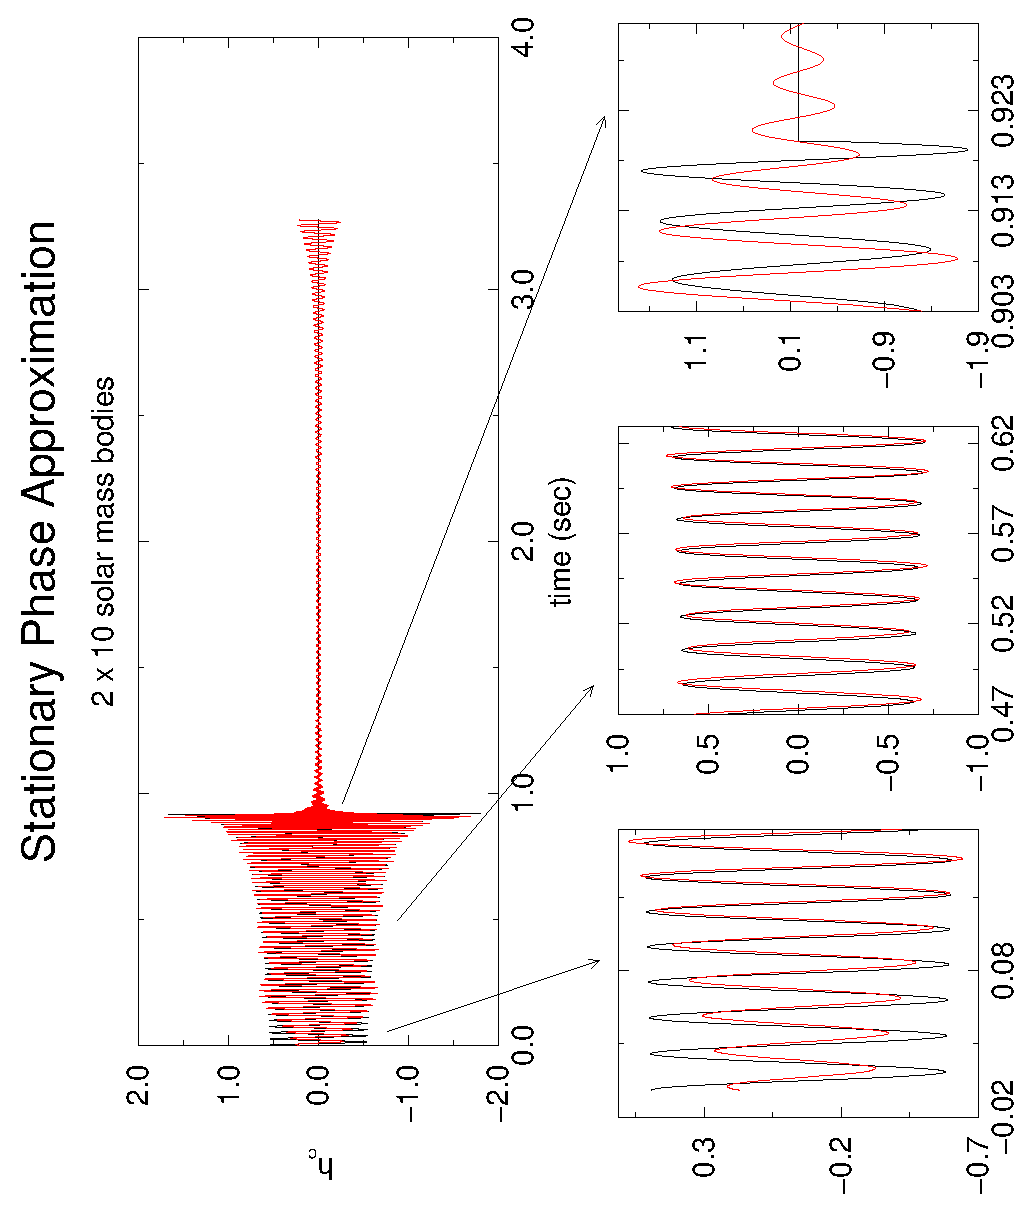
\epsfig{file=Figures/compare_chirps.ps,angle=-90,width=4.5in}
\caption{ \label{f:compare_chirps}
The output of {\tt compare\_chirps}, comparing the stationary-phase
approximate waveform FFT'd into the time domain (red curve) with a
2nd-order post-Newtonian chirp calculated in the time domain, using
{\tt make\_filters()} (black curve).  The lower part of the graph shows
three interesting regions of the upper (complete) graph.  The bottom
left detail shows the Gibbs startup-transient, the bottom middle detail
shows a typical region of good agreement, and the bottom right detail
shows the Gibbs turn-off transient.  The Gibbs startup transient is
also visible at the far right of the upper figure, which is
periodically identified with the far left.  }
\end{center}
\end{figure}



%%%%%%%%%%%%%%%%%%%%%%%%%%%%%%%%%%%%%%%%%%%%%%%%%%%%%%%%%%%%%%%%%%%%%%%%%%%%
%%%%%%%%%%%%%%%%%%    END OF BEN OWEN'S RESPONSIBILITY %%%%%%%%%%%%%%%%%%%%%
%%%%%%%%%%%%%%%%%%%%%%%%%%%%%%%%%%%%%%%%%%%%%%%%%%%%%%%%%%%%%%%%%%%%%%%%%%%%

\clearpage
\subsection{Wiener (optimal) filtering}
\label{ss:wienerfilt}
\setcounter{equation}0
The technique of {\it optimal filtering} is a well-studied and
well-understood technique which can be used to search for
characteristic signals (in our case, chirps) buried in detector noise.
In order to establish notation, we begin this section with a brief
review of the optimal filtering technique.

Suppose that the detector output is a dimensionless strain $h(t)$.  (In
Section~\ref{s:40meter} we show how to construct this quantity for the
CIT 40-meter prototype interferometer, using the recorded digital data
stream).  We denote by ${C}(t)$ the waveform of the signal (i.e.,
the chirp) which we hope to find, hidden in detector noise, in the
signal stream $h(t)$.  Since we would like to know about chirps which
start at different possible times $t_0$, we'll take ${C}(t) =
\alpha T(t-t_0)$ where $T(t)$ is the canonically normalized waveform 
of a chirp which enters the sensitivity band of the interferometer at 
time $t=0$. The constant $\alpha$ quantifies the strength of the signal
we wish to extract as compared to an otherwise identical signal of 
canonical strength (we will discuss how this canonical normalization
is defined shortly). In other words, $T(t)$ contains all the 
information about the chirp we are searching for apart from the 
arrival time and the strength, which are given by $t_0$ and $\alpha$ 
respectively. For the moment, we will ignore the fact that 
the chirps come in two different phase ``flavors".

We will construct a signal $S$, which is a number defined by
\begin{equation}
S = \int_{-\infty}^\infty dt \;h(t) Q(t),
\end{equation}
where $Q(t)$ is an optimal filter function in time domain, which we
will shortly determine in a way that maximizes the signal-to-noise
ratio $S/N$ or SNR.  We will assume that $Q$ is a real function of
time.

We use the Fourier transform conventions of (\ref{e:fft1}) and
(\ref{e:fft2}), in terms of which we can write the signal $S$ as
\begin{eqnarray}
\nonumber
S &=& \int_{-\infty}^\infty dt  \int_{-\infty}^\infty df  \int_{-\infty}^\infty df'
{\rm e}^{-2 \pi i f t+2 \pi i f' t} \tilde h(f) \tilde Q^* (f')\\
\nonumber
&=& 
\int_{-\infty}^\infty df  \int_{-\infty}^\infty df'
\delta(f-f') \tilde h(f) \tilde Q^* (f')\\
&=& 
\int_{-\infty}^\infty df \tilde h(f) \tilde Q^* (f).
\end{eqnarray}
This final expression gives the signal value $S$ written in the
frequency domain, rather than in the time domain.

Now we can ask about the expected value of $S$, which we denote 
$\langle S \rangle$. This is the average of $S$ over an ensemble of 
detector output streams, each one of which contains an identical 
chirp signal $C(t)$ but different realizations of the noise:
\begin{equation}
h(t) = C(t) + n(t).
\end{equation}
So for each different realization, $C(t)$ is exactly the same function,
but $n(t)$ varies from each realization to the next.  We will assume
that the noise has zero mean value, and that the phases are randomly
distributed, so that $\langle \tilde n(f) \rangle=0$.  We can then take
the expectation value of the signal in the frequency domain, obtaining
\begin{equation}
\langle S \rangle = \int_{-\infty}^\infty df \langle \tilde h(f)
\rangle \tilde Q^*(f) = \int_{-\infty}^\infty df \tilde C(f) \tilde
Q^*(f).
\end{equation}
We now define the {\it noise} $N$ to be the difference between the
signal value and its mean for any given element of the ensemble:
\begin{equation}
\label{e:noise}
N \equiv S-\langle S \rangle = \int_{-\infty}^\infty df \tilde n(f) \tilde Q^* (f).
\end{equation}
The expectation value of $N$ clearly vanishes by definition, so
$\langle N \rangle=0$.  The expected value of $N^2$ is non-zero,
however.   It may be calculated from the (one-sided) strain noise power
spectrum of the detector $S_h(f)$, which is defined by
\begin{equation}
\label{e:nspec}
\langle \tilde n(f) \tilde n^*(f') \rangle = {1 \over 2} S_h(|f|) \delta(f-f'),
\end{equation}
and has the property that 
\begin{equation}
\langle n^2(t) \rangle = \int_0^\infty S_h(f) \; df.
\end{equation}
We can now find the expected value of $N^2$, by squaring equation (\ref{e:noise}),
taking the expectation value, and using (\ref{e:nspec}), obtaining
\begin{eqnarray}
\nonumber
\langle N^2 \rangle &= & \int_{-\infty}^\infty df \int_{-\infty}^\infty
df' \tilde Q^*(f) \langle \tilde n(f)   \tilde n^*(f') \rangle \tilde
Q(f') \\
\nonumber
& = & {1 \over 2} \int_{-\infty}^\infty df \; S_h(|f|) |\tilde Q(f) |^2\\
\label{e:n2}
& = &  \int_{0}^\infty df \; S_h(f) |\tilde Q(f) |^2.
\end{eqnarray}
There is a nice way to write the formulae for the expected signal and
the expected noise-squared.  We introduce an ``inner product" defined
for any pair of (complex) functions $A(f)$ and $B(f)$.  The inner
product is a complex number denoted by $(A,B)$ and is defined by
\begin{equation}
\label{e:definprod}
(A,B) = \int_{-\infty}^\infty df \; {A(f) B^*(f) S_h(|f|)}.
\end{equation}
Because $S_h$ is positive, this inner product has the property that $(A,A)
\ge 0$ for all functions $A(f)$, vanishing if and only if $A=0$.  This
inner product is what a mathematician would call a ``positive definite
norm"; it has all the properties of an ordinary dot product of vectors
in three-dimensional Cartesian space.

In terms of this inner product, we can now write the expected signal, and the expected
noise-squared, as
\begin{equation}
\langle S \rangle = ({\tilde C \over S_h},\tilde Q)
\quad {\rm and} \quad \langle N^2 \rangle = {1 \over 2} (\tilde Q, \tilde Q).
\end{equation}
(Note that whenever $S_h$ appears inside the inner product, it refers
to the function $S_h(|f|)$ rather than $S_h(f)$.) Now the question is,
how do we choose the optimal filter function $Q$ so that the expected
signal is as large as possible, and the expected noise-squared is as
small as possible?  The answer is easy! Recall Schwarz's inequality for
inner products asserts that
\begin{equation}
        (A,B)^2 \le (A,A)(B,B),
\end{equation}
the two sides being equal if (and only if) $A$ is proportional to $B$.
So, to maximize the signal-to-noise ratio 
\begin{equation}
\label{e:sovern}
\left( {S \over N} \right)^2 ={\langle S \rangle^2 \over \langle N^2
\rangle} = 2 { ({\tilde C \over S_h},\tilde Q)^2 \over (\tilde Q,
\tilde Q)}
\end{equation}
we choose
\begin{equation}
\tilde Q(f) \propto {\tilde C(f) \over S_h(|f|)} = 
\alpha {\tilde T(f) \over S_h(|f|)} \; {\rm e}^{2 \pi i f t_0}.
\end{equation}
The signal-to-noise ratio defined by equation (\ref{e:sovern}) is normalized
in a way that is generally accepted and used.  Note that the definition is
independent of the normalization of the optimal filter $\tilde Q$, since
that quantity appears quadratically in both the numerator and denominator.
However if we wish to speak about ``Signal" values rather than about
signal-to-noise values, then the normalization of $\tilde Q$ is relevant.
If we choose the constant of proportionality to be $2 \alpha^{-1}$,
(i.e. set $\alpha = 2$, for reasons we will discuss shortly) then we
can express the template in terms of the canonical waveform,
\begin{equation}
\label{e:optimal}
        \tilde{Q}(f)=2 \> \frac{\tilde{T}(f)}{S_h(|f|)} {\rm e}^{2\pi i f t_0}
\end{equation}
Going back to the definition of our signal $S$, you will notice that the
signal $S$ for ``arrival time offset" $t_0$ is given by
\begin{eqnarray}
\nonumber
S &=& \int_{-\infty}^\infty df \; \tilde h(f) \tilde Q^* (f) \\
\label{e:lag}
  &=& 2 \int_{-\infty}^\infty df \; { \tilde h(f) \tilde T^* (f) 
\over S_h(|f|)} \; {\rm e}^{- 2 \pi i f t_0}.
\end{eqnarray}
Given a template $\tilde T$ and the signal $\tilde h$, the signal
values can be easily evaluated for any choice of arrival times $t_0$ by
means of a Fourier transform (or FFT, in numerical work).  Thus, it is
not really necessary to construct a different filter for each possible
arrival time; one can filter data for all possible choices of arrival
time with a single FFT.

The signal-to-noise ratio for this optimally-chosen filter can be
determined by substituting the optimal filter (\ref{e:optimal}) into
equation (\ref{e:sovern}), obtaining
\begin{equation}
\nonumber
\left( {S \over N} \right)^2 = 
 2 \int_{-\infty}^\infty df {| \tilde C(f) |^2 \over S_h(|f|)} =
 4 \int_{0}^\infty df { | \tilde C(f) |^2 \over S_h(f)} = 2 \alpha^2 
 \left(\frac{\tilde{T}}{S_h(|f|)},\frac{\tilde{T}}{S_h(|f|)}\right).
\end{equation}
You will notice that the signal-to-noise ratio $S/N$ in
(\ref{e:sovern}) is independent of the overall normalization of the
filter $Q$:  if we make $Q$ bigger by a factor of ten, both the
expected signal and the expected noise increase by exactly the same
amount.  For this reason, we can specify the normalization of the 
filter as we wish. Furthermore, it is obvious from (\ref{e:optimal}) 
that normalizing the optimal filter is equivalent to specifying the
normalization of the canonical signal waveform. It is traditional
(for example in Cutler and Flanagan \cite{cutler:1994})
to choose 
\begin{equation}
\label{e:cfnorm}
   \left(\frac{\tilde{T}}{S_h(|f|)},\frac{\tilde{T}}{S_h(|f|)}
   \right)=\frac{1}{2}.
\end{equation}
With this normalization, 
the expected value of the squared noise is
\begin{equation}
\langle N^2 \rangle = {1 \over 2} (\tilde Q,\tilde Q) = {1 \over 2} \>
\left( 2 \frac{\tilde{T}}{S_h(|f|)},2 \frac{\tilde{T}}{S_h(|f|)}
   \right) = 1
\end{equation}
and the signal-to-noise ratio takes the simple form
\begin{equation}
\left(\frac{S}{N}\right)^2 = \alpha^2.
\end{equation}
This adjustment or change of the filter normalization can be obtained 
by moving the (fictitious) astrophysical system emitting the chirp 
template either closer or farther away from us.  Because the metric 
strain $h$ falls off as $1/\rm distance$, the measured signal strength 
$S$ is then a direct measure of the inverse distance.

For example, consider a system composed of two  1.4 $M_\odot$ masses in
circular orbit.  Let us normalize the filter $\tilde T$ so that equation
(\ref{e:cfnorm}) is satisfied.  This normalization corresponds to placing
the binary system at some distance.  For the purpose of discussion,
suppose that this distance is 15 megaparsecs (i.e., choosing $T(t)$
to be the strain produced by an optimally-oriented two $\times$ 1.4
$M_\odot$ system at a distance of 15 megaparsecs).  If we then detect
a signal with a signal-to-noise ratio $S/N=30$, this corresponds to
detecting an optimally-oriented source at a distance of half a megaparsec.
Note that the normalization we have choosen has the r.m.s. noise $\sqrt{
\langle N^2 \rangle}= 1$ and therefore the signal and signal-to-noise
values are equal.

The functions {\tt correlate()} and {\tt productc()} are designed to
perform this type of optimal filtering.  We document these routines in
the following section and in Section~\ref{s:utility}, then provide a simple
example of an optimal filtering program.

There is an additional complication, arising from the fact that the
gravitational radiation from a binary inspiral event is a linear
combination of two possible orbital phases, as may be seen by reference
to equations (\ref{e:chirpcos}) and (\ref{e:chirpsin}).  Thus, the
strain produced in a detector is a linear combination of two waveforms,
corresponding to each of the two possible ($0^\circ$ and $90^\circ$)
orbital phases:
\begin{equation}
h(t) = \alpha T_{0}(t) + \beta T_{90}(t) + n(t).
\end{equation}
Here the subscripts $0$ and $90$ label the two possible orbital phases;
the constants $\alpha$ and $\beta$ depend upon the distance to the source
(and the normalization of the templates) and the orientation of the source
relative to the detector.  Thus $ T_{0}(t) $ denotes the (suitably
normalized) function $h_c(t)$ given by equation (\ref{e:chirpcos})
and $ T_{90}(t) $ denotes the (suitably normalized) function $h_s(t)$
given by equation (\ref{e:chirpsin}).

In the optimal filtering, we are now searching for a pair of amplitudes
$\alpha$ and $\beta$ rather than just a single amplitude.  One can easily do
this by choosing a filter function which corresponds to a complex-valued signal
in the time-domain:
\begin{equation}
\tilde Q(f) =   2 \>
{\tilde T_{0}(f) - i \tilde T_{90}(f) \over S_h(|f|)} \; {\rm e}^{2 \pi i f t_0}.
\end{equation}
We will assume that the individual filters for each polarization are
normalized by the convention just described, and that they are orthogonal:
\begin{equation}
\label{e:ono}
\left( {\tilde T_{0} \over S_h} , {\tilde T_{0} \over S_h} \right) = 
\frac{1}{2}, {\rm \ and\ }
\left( {\tilde T_{90} \over S_h} , {\tilde T_{90} \over S_h} \right) = 
\frac{1}{2}, {\rm \ and\ }
\left( {\tilde T_{0} \over S_h} , {\tilde T_{90} \over S_h} \right) = 0.
\end{equation}
Note that $T_{0}$ and $T_{90}$ are only exactly orthogonal in the
adiabatic limit where they each have many cycles in any frequency
interval $df$ in which the noise power spectrum $S_h(f)$ changes
significantly.  Also note that the filter function $\tilde Q(f)$ does
not correspond to a real filter $Q(t)$ in the time domain, since
$\tilde Q(-f) \ne \tilde Q^*(f)$, so that the signal
\begin{equation}
\label{e:complexsig}
S(t_0) = \left( {  \tilde h \over S_h}, \tilde Q \right)
\end{equation}
is a complex-valued functions of the lag $t_0$.  We define the noise as
before, by $N= S - \langle S \rangle$.  Its mean-squared modulus is
\begin{eqnarray}
\nonumber
\langle | N | ^2 \rangle &=& {1 \over 2} (\tilde Q,\tilde Q) \\
\nonumber
& = & 2 \left( {\tilde T_{0} -i \tilde T_{90} \over S_h} ,  
{\tilde T_{0} -i \tilde T_{90} \over S_h} \right) \\
& = & 2 \left[ \left( 
{\tilde T_{0} \over S_h} , {\tilde T_{0}  \over S_h} \right) +
\left( {\tilde T_{90}   \over S_h} , {\tilde T_{90}  \over S_h} \right) \right] = 2,
\end{eqnarray}
where we have made use of the orthornormality relation (\ref{e:ono}).
This value is twice as large as the expected noise-squared in the case of a single
phase waveform considered previously.

The expected signal at zero lag $t_0=0$ is
\begin{equation}
\langle S \rangle = \left( { \langle \tilde h \rangle \over S_h}, \tilde Q \right) =
2 \left( {\alpha \tilde T_{0}  + \beta \tilde T_{90} \over S_h} ,  
{\tilde T_{0} -i \tilde T_{90} \over S_h} \right) =  
\alpha +  i \beta.
\end{equation}
Hence the signal-to-noise ratio is
\begin{equation}
{\langle S \rangle \over \sqrt{\langle |N|^2 \rangle} } = \frac{1}{\sqrt{2}}
(\alpha + i \beta).
\end{equation}
In the absence of a signal $\langle S \rangle=0$ the expected value of the square of
this quantity (from the definition of $N$) is unity:
\begin{equation}
{\langle |S|^2 \rangle \over \langle |N|^2 \rangle} = 1.
\end{equation}
In the presence of a signal, the squared signal-to-noise ratio is
\begin{equation}
{| \langle S  \rangle |^2 \over \langle |N|^2 \rangle} = \frac{1}{2}
(\alpha^2 + \beta^2)
\end{equation}
In the case discussed previously, for a single-phase signal, we pointed out that
there was general agreement on the definition of signal-to-noise value.  In the present
case (a complex or two-phase signal) there is no such agreement.  The definition given
above is the one used by most experimenters: it is a quantity whose square has expected value
of unity in the absence of a signal.  However the definition often used in this
subject is
\begin{equation}
\left( {S \over N} \right)_{\rm Cutler\ and\ Flanagan} =
\left( {S \over N} \right)_{\rm Owen} =
\left( {S \over N} \right)_{\rm Thorne} = \max_{t_0} | S(t_0) |=
\sqrt{2} \left( {S \over N} \right)_{\rm GRASP}.
\end{equation}
Note that because ${S(t_0)}$ is complex, we maximize the modulus.
This is a quantity whose expected squared value, in the absence of a
signal, is 2.  To avoid confusion in the future, we will use a different
symbol for this quantity, and define
\begin{equation}
\rho \equiv 
\left( {S \over N} \right)_{\rm Cutler\ and\ Flanagan} =
\left( {S \over N} \right)_{\rm Owen} =
\left( {S \over N} \right)_{\rm Thorne} =
\sqrt{2} \left( {S \over N} \right)_{\rm GRASP}.
\end{equation}
This quantity is equal to the signal value alone (rather than the signal
value divided by the expected noise).

Another way to understand these two different choices of normalization,
and to understand why the conventional choice of normalization is $\rho$,
is that conventionally one treats the two-phase case in the same way
as the single phase case, but regards ${S \over N}$ as a function of a
phase parameter, $\theta = \arctan(\beta/\alpha)$.  For any fixed $\theta$,
${S \over N}(\theta)$ has rms value one, but the statistic $\max_\theta
{S \over N} (\theta)$ has rms value $\sqrt{2}$.

The attentive reader will notice, with our choice of filter and
signal normalizations, that we have lost a factor of $\sqrt{2}$ in the
signal-to-noise ratio compared to the case where we were searching for
only a single phase of waveform.  The expected signal strength in the
presence of a 0-phase signal is the same as in the single-phase case,
but the expected (noise)${}^2$ has been doubled.  This is because of the
additional uncertainty associated with our lack of information about the
relative contributions of the two orbital phases.  In other words, if we
know in advance that a waveform is composed entirely of the zero-degree
orbital phase, then the expectation value of the signal-to-noise,
determined by equation (\ref{e:sovern}) would be given by $\langle S
\rangle/N = \sqrt{2} \alpha$.  However if we need to search for the
correct linear combination of the two possible phase waveforms, then
the expectation value of the signal-to-noise is reduced to  $\langle
S \rangle/N = \alpha$.  However, as we will see in the next section,
this reduction in signal-to-noise ratio does not significantly affect
our ability to detect signals with a given false alarm rate.
\clearpage

\subsection{Comparison of signal detectability for single-phase and two-phase searches}
\label{ss:compare12}
The previous Section \ref{ss:wienerfilt} described optimal filtering searches in two cases -
looking for:
\begin{itemize}
\item 
A signal of known phase, proportional to $T_0$, and
\item
A signal of unknown phase, which is some linear
combinations of $T_0$ and $T_{90}$.
\end{itemize}
With the choice of filter normalizations made previously, the expected
signal produced by a source $\alpha T_0$ would be the same for both
searches, but the expected (noise)${}^2$ was higher in the two-phase case.
One might wonder if this reduced SNR means that a two-phase search reduces
ones ability to identify signals.  The answer turns out to be ``not significantly".

The reason for this is that the distribution of signal values produced
by detector noise alone in the single- and two-phase cases are quite
different.  In order to answer the question: ``what is the smallest
signal detectable" we need to fix a false alarm rate.  For a given
time-duration of data, this is equivalent to fixing a false alarm
probability.  Let us assume that this probability has been fixed to be
a small value $\epsilon$, and compare the single- and two-phase searches.

In the single-phase case, in the absence of a source, the values of
the signal $S$ (\ref{e:lag}) are Gaussian random variables with a
mean-squared value of 1.  Hence the threshold $S_0$ determined by the
false alarm rate must be set so that there is probability $\epsilon$
of $S$ falling outside the range $[-S_0,S_0]$.  This means that
\begin{equation} \epsilon = 2 {1 \over
\sqrt{2 \pi}} \int_{S_0}^\infty \exp(-x^2/2) \> dx = {\rm \ erfc} (S_0/\sqrt{2}) .
\end{equation}
The solution to this equation is the threshold as a function of the false alarm
probability:
\begin{equation}
S_0^{\small \textrm{single-phase}}(\epsilon)=\sqrt{2}
{\rm \ erfc}^{-1}(\epsilon).
\end{equation}
Thus, for example, to obtain a false alarm probability of $\epsilon =
10^{-5}$ we need to set a threshold $S^{\small \textrm{single-phase}}_0
= \sqrt{2} \textrm{\ erfc}^{-1}(10^{-5}) = 4.417$.  In this case, our
minimum detectable signal has amplitude $\alpha = 4.417$.

In the two-phase case, the probability distribution of the signal in
the absence of a source is different, because in this case the signal
(\ref{e:complexsig}) is described by the probability distribution of
a random variable $r$, where $r^2 = x^2 + y^2$ and $x$ and $y$ are
independent random Gaussian variables with unit rms.   Here, $x$ and
$y$ are the real and imaginary parts of the signal (\ref{e:complexsig}
in the absence of a source.  Their probability distribution is:
\begin{eqnarray}
\nonumber
P(x) dx P(y) dy & = & {1 \over 2 \pi} {\rm e}^{-x^2/2} {\rm e}^{-y^2/2} dx dy \\
                & = & {1 \over 2 \pi} {\rm e}^{-r^2/2} r dr d\phi \\
\nonumber
   & \Rightarrow  &\\
   P(r)dr & = &  {\rm e}^{-r^2/2} r dr.
\end{eqnarray}
In the final line, we have integrated over the irrelevant angular variable
$\phi \in [0,2\pi)$.  So in the two-phase case, as before, the threshold value of the
signal is set by requiring that the false alarm probability be $\epsilon$:
\begin{equation}
\epsilon=\int_{S_0}^\infty \exp(-r^2/2) r dr = \exp({-S_0^2/2}).
\end{equation}
The solution here is that the threshold is
$S^{\small \textrm{two-phase}}_0 = \sqrt{-2  \ln
\epsilon}$.  For example, to obtain a false alarm probability of $\epsilon
= 10^{-5}$ we need to set a threshold $S^{\small \textrm{two-phase}}_0 = 4.799$.  In this case,
our minimum detectable (0-phase) signal has amplitude $\alpha = 4.799$,
which is only slightly higher than in the single-phase case.

It is not a coincidence that for a given false alarm rate, the amplitude
of the minimum detectable signals are almost the same.  Although the
expected value of the single-phase signal${}^2$ in the absence of a source
is smaller than the expected value of the two-phase $|{\rm signal}|^2$
in the absence of a source, the {\it tails} of the two probability
distributions are almost identical.  For the same false alarm probability
$\epsilon$ the thresholds in the two instances are related by
\begin{equation}
\epsilon=
\sqrt{2 \over \pi} \int_{S^{\small \textrm{single-phase}}_0}^\infty \exp(-x^2/2) \>dx
=
\int_{S^{\small \textrm{two-phase}}_0}^\infty \exp(-r^2/2) r dr
\end{equation}
But for thresholds of reasonable size (small $\epsilon$) both integrals
are dominated by the region just to the right of $S_0$, and in this neighborhood the
integrands differ by a small factor of approximately $\sqrt{\pi S_0 \over 2}$.
Since $\epsilon$ varies exponentially with the threshold, there is a logarithmically
small difference between the thresholds $S^{\small \textrm{single-phase}}_0$ and
$S^{\small \textrm{two-phase}}_0$.

For a fixed false alarm probability, we can write the the two-phase
threshold $S^{\small \textrm{two-phase}}_0$ as a function of the
one-phase threshold $S^{\small \textrm{single-phase}}_0$:
\begin{equation}
S^{\small \textrm{two-phase}}_0 = \sqrt{ - 2 \ln \left(\textrm{erfc}\left({S^{\small \textrm{single-phase}}_0 \over \sqrt{2}}\right) \right)}.
\end{equation}
The plot of this relationship in Figure \ref{f:thresholds} shows clearly
that once the thresholds are reasonably large, they are very nearly equal.
\begin{figure}[h]
\begin{center}
\epsfig{file=Figures/thresholds.ps,angle=0,width=3.5in}
\caption{ \label{f:thresholds} The threshold for a two-phase search
$S^{\small \textrm{two-phase}}_0$ is shown as a function of the threshold
for the single-phase search $S^{\small \textrm{single-phase}}_0$ which
gives the same false alarm rate.  When the false alarm rates are small,
they are very nearly equal.  }
\end{center}
\end{figure}

\clearpage

\subsection{Function: \tt correlate()}
\label{ss:correlate}
\setcounter{equation}0
{\tt void correlate(float *s,float *h,float *c,float *r,int n)}\\
This function evaluates the correlation (as a function of lag time $t$)
defined by the discrete equivalent of equation (\ref{e:lag}):
\begin{equation}
\label{e:corrdef}
s(t) = {1 \over 2} \int_{-\infty}^\infty df \; { \tilde h(f) \tilde c^* (f) \tilde r (f) }
 \; {\rm e}^{- 2 \pi i f t}.
\end{equation}
It is assumed that $\tilde h(f)$ and $\tilde c(f)$ are Fourier
transforms of real functions, and that $\tilde r(f)$ is real.  The factor of
$1/2$ appears in (\ref{e:corrdef}) for efficiency reasons; in order to calculate
the integral (\ref{e:lag}) one should set $\tilde r(f) = 2/S_h(f)$.  The routine
assumes that $\tilde r$ vanishes at both DC and the Nyquist frequency.

The arguments are:
\begin{description}
\item{\tt s}: Output.  Upon return, the array {\tt s[0..n-1]} contains
  the correlation $s(t)$ at times 
  \begin{equation}
   \nonumber
    t=0,\Delta t, 2 \Delta t,\cdots,(n-1) \Delta t.
  \end{equation}
\item{\tt h}: Input.  The array {\tt h[0..n-1]} contains the positive
  frequency ($f \ge 0$) part of the complex function $\tilde h(f)$.
  The packing of $\tilde h$ into this array follows the scheme used by
  the {\it Numerical Recipes} routine {\tt realft()}, which is
  described between equations (12.3.5) and (12.3.6) of \cite{NumRec}.
  The DC component $\tilde h(0)$ is real, and located in {\tt h[0]}.
  The Nyquist-frequency component $\tilde h(f_{\rm Nyquist})$ is also
  real, and is located in {\tt h[1]}.  The array elements {\tt h[2]}
  and {\tt h[3]} contain the real and imaginary parts, respectively, of
  $\tilde h(\Delta f)$ where $\Delta f = 2 f_{\rm Nyquist}/n = (n
  \Delta t)^{-1}$.   Array elements {\tt h[2j]} and {\tt h[2j+1]}
  contain the real and imaginary parts of $\tilde h( j \; \Delta f)$
  for $j=1,\cdots,n/2-1$.  It is assumed that $\tilde h(f)$ is the
  Fourier transform of a real function, so that {\tt correlate()} can
  infer the negative frequency components from the equation $\tilde
  h(-f) = \tilde h^*(f)$
\item{\tt c}: Input.  The array {\tt c[0..n-1]} contains the complex
  function $\tilde c$, packed in the same format as $\tilde h(f)$,
  with the same assumption that $\tilde c(-f) = \tilde c^*(f)$.
  Note that while you provide the function $\tilde c(f)$ to the
  routine, it is the {\it complex-conjugate} of the function contained
  in the array {\tt c[ ]} which is used in calculating the correlation.
  Thus if $\tilde r$ is positive, {\tt correlate(s,c,c,r,n)} will
  always return ${\tt s[0]}\ge 0$.
\item{\tt r}: Input.  The array {\tt r[0..n/2]} contains the values of
  the real function $\tilde r$ used as a weight in the integral.  This
  is often chosen to be (twice!) the inverse of the receiver noise, as
  in equation (\ref{e:lag}), so that $\tilde r(f) = 2/\tilde
  S_h(|f|)$.  The array elements are arranged in order of increasing
  frequency, from the DC value at subscript 0, to the Nyquist frequency
  at subscript n/2.  Thus, the $j$'th array element {\tt r[j]} contains
  the real value $\tilde r(j \; \Delta f)$, for $j=0,1,\cdots,n/2$.
  Again it is assumed that $\tilde r(-f) = \tilde r^*(f) = \tilde r(f)$.
\item{\tt n}: Input.  The total length of the complex arrays
  {\tt h} and {\tt c}, and the number of points in the output
  array {\tt s}.  Note that the array {\tt r} contains $n/2+1$
  points.  n must be even.
\end{description}
The correlation function calculated by this routine is ${1 \over 2} FFT^{-1}[\tilde
h \tilde c^* \tilde r]$ and has the same dimensions as the product
$\tilde h \times \tilde c \times \tilde r$.  The definition is
\begin{equation}
{\tt s}_k = {1 \over 2} \sum_{j=0}^{{\tt n}-1} {\tt h}_j {\tt c}^*_j {\tt r}_j
{\rm e}^{- 2 \pi i j k/{\tt n}}
\end{equation}
where it is understood that ${\tilde h}_{{\tt n}-j} = \tilde h^*_j$ and
that ${\tilde c}_{{\tt n}-j} = \tilde c^*_j$, and that
${\tilde r}_{{\tt n}-j} = \tilde r_j$. 

Note that the input arrays
{\tt h[ ]} and {\tt c[ ]} can be the same array.  For example {\tt
correlate(s,c,c,r,n)} calculates the discrete equivalent of
\begin{equation}
s(t) = {1 \over 2} \int_{-\infty}^\infty df \; { |\tilde c (f) |^2 \tilde r (f) }
 \; {\rm e}^{- 2 \pi i f t}.
\end{equation}

\begin{description}
\item{Author:}
Bruce Allen, ballen@dirac.phys.uwm.edu
\item{Comments:}
For the sake of efficiency, this function does not include the
contribution from either DC or Nyquist frequency bins to the
correlation (these are negligible in any sensible data).
\end{description}
\clearpage

\subsection{Function: {\tt avg\_inv\_spec()}}
\label{ss:avg_inv_spec}
\setcounter{equation}0
{\tt  void avg\_inv\_spec(float flo,float srate,int n,double decay,double *norm,
                  float *htilde, float* mean\_pow\_spec,float* twice\_inv\_noise)}\\
This function maintains an auto-regressive moving average (see {\tt
avg\_spec()}) of the power spectrum $S_h(f)$, and an array containing
$2/S_h(f)$, which can be used for optimal filtering.  This latter array
is set to zero below a specified cuff-off frequency $f_{low}$.

The arguments are:
\begin{description}
\item{\tt flo:} Input.  The low frequency cut-off $f_{low}$, in Hz.
\item{\tt srate:} Input.  The sample rate, in Hz.
\item{\tt n:} Input.  The number of points in the arrays.
\item{\tt decay:} Input.  The quantity $\exp(-\alpha)$ as defined in {\tt avg\_spec()}.
  Sets the characteristic decay time for the auto-regressive average.
\item{\tt norm:} Input/Ouput.  Used for internal storage.  Set to $0$ when you want to begin
   a new auto-regressive average.  Must not be altered otherwise.
\item{\tt htilde:} Input.  The array {\tt htilde[0..n-1]} contains the positive frequency FFT of
   the metric perturbation.
\item{\tt mean\_pow\_spec:} Output.  The array {\tt mean\_pow\_spec[0..n/2]} contains the 
  mean power spectrum.  Should be zeroed when resetting to begin a new average.  The array
element {\tt mean\_pow\_spec[0]} contains the power spectrum at DC, and the array
element {\tt mean\_pow\_spec[n/2]} contains the power spectrum at the Nyquist frequency
{\tt srate}/2.
\item{\tt twice\_inv\_noise:} Output.  The array {\tt
   twice\_inv\_noise[0..n/2]} contains $2/S_h(f)$.  It is set to zero for
   $f<f_{low}$.  The array element {\tt twice\_inv\_noise[0]} contains
   the DC value, and the array element {\tt twice\_inv\_noise[n/2]}
   contains the value at the Nyquist frequency {\tt srate}/2.
\end{description}
\begin{description}
\item{Author:}
Bruce Allen, ballen@dirac.phys.uwm.edu
\item{Comments:}
We assume here that the ``correct" thing to do is the average the
spectrum, then invert it.  There may be a better way to construct
the weight function for an optimal filter, however.
\end{description}
\clearpage

\subsection{Function: {\tt orthonormalize()}}
\label{ss:orthonormalize}
\setcounter{equation}0
{\tt void orthonormalize(float* ch0tilde, float* ch90tilde, float* twice\_inv\_noise, int n, float* n0, float* n90)}\\
This function takes as input the (positive frequency parts of the) FFT
of a pair of chirp signals.  Upon return, the $90^\circ$ phase chirp
has been made orthogonal to the $0^\circ$ phase chirp, with respect to
the inner product defined by $2/S_h$.  The normalizations of the chirps
are also returned.

The arguments are:
\begin{description}
\item{\tt ch0tilde:} Input.  The FFT of the zero-phase chirp $T_0$.
\item{\tt ch90tilde:} Input/Output.  The FFT of the $90^\circ$-phase chirp $T_{90}$.
\item{\tt twice\_inv\_noise:} Input.  Array containing $2/S_h$.
The array element {\tt twice\_inv\_noise[0]} contains
   the DC value, and the array element {\tt twice\_inv\_noise[n/2]}
   contains the value at the Nyquist frequency.
\item{\tt n:} Input. Defines the length of the arrays: {\tt ch0tilde[0..n-1]}, {\tt ch90tilde[0..n-1]},
  and {\tt twice\_inv\_noise[0..n/2]}.
\item{\tt n0:} Output.  The normalization of the 0-phase chirp.
\item{\tt n90:} Output.  The normalization of the $90^\circ$-phase chirp.
\end{description}

Using the notation of (\ref{e:definprod}) one may define an inner product of the
chirps.  The normalizations are defined as follows:
\begin{equation}
{1 \over n_0^2} \equiv {1 \over 2} (Q_0,Q_0),
\end{equation}
where $Q_0$ is the optimal filter defined for the zero-phase chirp $T_0$.
The chirps are orthogalized internally using the Gram-Schmidt procedure.
We first calculate $(Q_0,Q_0)$ and $(Q_{90},Q_{0})$ then define
$\epsilon = (Q_{90},Q_{0})/(Q_0,Q_0)$.  We then modify the $90^\circ$-phase chirp
setting
$\tilde T_{90} \rightarrow T_{90} - \epsilon T_0$.  This ensures that the
inner product $(Q_{90},Q_{0})$ vanishes.  The normalization for this newly-defined
chirp is then defined by
\begin{equation}
{1 \over n_1^2} \equiv {1 \over 2} (Q_{90},Q_{90}).
\end{equation}
\begin{description}
\item{Author:}
Bruce Allen, ballen@dirac.phys.uwm.edu
\item{Comments:}
Notice that the filters $Q_0$ and $Q_{90}$ are not in general
orthogonal except in the adiabatic limit as $S_h(f)$ varies very slowly
with changing $f$.  Our approach to this is to construct a
slightly-modified ninety-degree phase signal.  Note however that this
may introduce small errors in the determination of the orbital phase.
This should be quantified.
\end{description}
\clearpage


\subsection{Dirty details of optimal filtering: wraparound and windowing}
\label{ss:dirty}
To carry out optimal filtering, we need to break the data set (which
might be hour, days, or weeks in length) into shorter stretches of $N$
points (which might be seconds or minutes in length). We can understand
the effects of ``chopping up" the data most easily in the case for
which (1) the instrument noise is {\it white}, so that $S_h(f)=1$; (2)
the source is so close that its signal overwhelms the noise in the
IFO, and (3) we are looking for a signal with a given phase (not a
linear combination of the two orbital phases).

We want to calculate a signal $S$ as a function of lag $t_0$ using
an FFT.
\begin{equation}
S(t_0) = \int h(t) T(t-t_0) dt \approx
S(i_0) = \sum_j h_j T_{j-i_0},
\end{equation}
where we have written both the continuous-time and discrete-time version
of the same equation.  Using the definition of the discrete Fourier
transform, and writing
\begin{equation}
h_j = \sum_{k=0}^{N-1} {\rm e}^{-2 \pi i j k/N} \tilde h_k \quad
{\rm and } \quad
T_{j-i_0} = \sum_{k'=0}^{N-1} {\rm e}^{-2 \pi i (j-i_0) k'/N} \tilde T_{k'} \quad
\end{equation}
one can easily compute that the signal as a function of lag $i_0$
is
\begin{eqnarray}
S(i_0) &=& \sum_{j=0}^{N-1} \sum_{k=0}^{N-1} \sum_{k'=0}^{N-1}
{\rm e}^{-2 \pi i j k/N} \tilde h_k 
{\rm e}^{-2 \pi i (j-i_0) k'/N} \tilde T_{k'} \\ 
&=& \sum_{k=0}^{N-1} \sum_{k'=0}^{N-1} N \delta_{k,-k'} 
{\rm e}^{2 \pi i i_0 k'/N} \tilde h_k \tilde T_{k'} \\
&=& \sum_{k=0}^{N-1}   N   
{\rm e}^{-2 \pi i i_0 k/N} \tilde h_k \tilde T^*_{k}.
\end{eqnarray}
Thus, if the data is treated as periodic, and the template is treated as
periodic, one can compute the correlation as a function of time using only
an FFT.  In particular, the use of rectangular windowing does create
sidelobes of the template's frequency components.  However it also creates
identical sidelobes of the signal's frequency components - so in effect the
correlation in the time domain can be calculated exactly, without any windowing
of the signal being necessary.

The only complication arises from the fact that the FFT treats the data
as being periodic.  Let's consider some simple examples to illustrate
the effects of this.   In all of our examples, the number of data
points is $N=65,536=2^{16}$ and the (schematic) chirp filter has length
$m=13,500$ and is zero-padded after that time.   Please remember, in
all the figures that follow, to identify the far right hand side of the
graph ($i=65535$) with the far left hand side ($i=0$).
Figure~\ref{f:chirpa} shows $S(i_0)$ for a schematic chirp which begins
at the first data point in the rectangular window.  You will notice
that the filter output peaks at $i=0$.
\begin{figure}[h]
\index{colorpage}
\begin{center}
\epsfig{file=Figures/fig12a.ps,angle=-90,width=4.5in}
\caption{ \label{f:chirpa} A chirp starting at initial time $i=0$ and
ending at time $i=13500$ is processed through a chirp filter, whose
output peaks at time $i=0$.  Notice that because of wraparound, the
(non-causal) filter output begins ``earlier" than $i=0$.}
\end{center}
\end{figure}
If the incoming chirp arrives somewhat later (it starts at $i=15,000$)
as shown in Figure~\ref{f:chirpb} then the filter output peaks at the
start time, as shown.
\begin{figure}[h]
\index{colorpage}
\begin{center}
\epsfig{file=Figures/fig12b.ps,angle=-90,width=4.5in}
\caption{ \label{f:chirpb} A chirp starting at initial time $i=15,000$ and
ending at time $i=28,500$ is processed through a chirp filter, whose
output peaks at time $i=15,000$.}
\end{center}
\end{figure}
A chirp in the signal which starts at the $i=65,535-13,500$ as shown in
Figure~\ref{f:chirpc} causes the filter output to peak at $i=52,035$.
\begin{figure}[h]
\begin{center}
\epsfig{file=Figures/fig12c.ps,angle=-90,width=4.5in}
\index{colorpage}
\caption{ \label{f:chirpc} A chirp starting at initial time $i=52,035$.}
\end{center}
\end{figure}
Thus, in order to find chirps, we need to find the maxima of the filter
output over the interval $i=0\cdots,N-m$.

Chirp filters can be ``stimulated" or ``triggered" by events that are
not chirps.  We will shortly discuss some techniques that can be used
to distinguish triggering events that are chirps from those that are
simply noise spikes or other transient (but non-chirp) varieties of
non-stationary interferometer noise.  Suppose that a chirp filter is
triggered by some kind of transient event in the IFO output.  At what
time did this transient event ocurr?  The answer to this question can
be seen by examining the impulse response of the ``periodic filter"
scheme, as shown in the following figures.
\begin{figure}[h]
\begin{center}
\epsfig{file=Figures/fig12d.ps,angle=-90,width=4.5in}
\index{colorpage}
\caption{ \label{f:chirpd} An impulse shortly after $i=0$.}
\end{center}
\end{figure}
\begin{figure}[h]
\begin{center}
\epsfig{file=Figures/fig12e.ps,angle=-90,width=4.5in}
\index{colorpage}
\caption{ \label{f:chirpe} An impulse at $i=15,000$.}
\end{center}
\end{figure}
\begin{figure}[h]
\begin{center}
\index{colorpage}
\epsfig{file=Figures/fig12f.ps,angle=-90,width=4.5in}
\caption{ \label{f:chirpf} An impulse at $i=28,500$.}
\end{center}
\end{figure}
\begin{figure}[h]
\begin{center}
\epsfig{file=Figures/fig12g.ps,angle=-90,width=4.5in}
\index{colorpage}
\caption{ \label{f:chirpg} An impulse shortly before $i=65535$}
\end{center}
\end{figure}
Thus, by searching for maxima in the filter output over the range
$i=0,\cdots,N-m-1$ we can detect either true chirps in the data stream,
starting in the time interval $i=0,\cdots,N-m-1$ and coalescing
(roughly speaking) in the time interval $i=m,\cdots, N-1$, or we can
detect transient impulse-like events in the data stream, which take
place in the time interval $i=m,\cdots, N-1$.  In the GRASP optimal
filtering code, after examining the stretch of $N$ data points, we then
shift the data points $i=N-m,\cdots,N-1$ into the range
$i=0,\cdots,m-1$ and acquire a new additional set of $N-m$ data points
covering remaining (new) time interval.

To indicate the time at which the filter output reached its maximum,
several different conventions can be used.  First, we can indicate the
{\it peak offset}.  This is the offset from the start of the filter output
at which the filter output reaches a maximum value.  Alternatively,
we can use the {\it impulse offset}.  This is the
offset at which the filter would have peaked if the maximum were due
to a delta-function like impulse at the input. These quantities
are defined in equation (\ref{e:impulsevspeak}).

Note that in practice, because the chirp signal has to be convolved
with the response function $R(f)$ of the detector, the impulse response
of the filter is typically a few points longer than the actual chirp
signal.  For this reason it is smart to assume that the impulse
response of your optimal filter is slightly longer (say a hundred
points longer) than the actual time-domain length of the corresponding
chirp.  This safety margin is set with the
{\tt {\#d}efine SAFETY} statement in the optimal filtering example.
You lose a tiny bit of efficiency but reduce the likelihood
that boundary effects from the data discontinuity at the start/end of
the rectangular window will significantly stimulate the optimal filter
output for $i=0,\cdots,N-m-1$. (See Figs.~\ref{f:chirpd} and
\ref{f:chirpg} to see an illustration of how this windowing
discontinuity will corrupt the filter's output.)

We have demonstrated explicitly that with no windowing (or rather,
rectangular windowing) of the data, one can find the appropriate
correlation between the signal and a filter exactly: the rectangular
window has the same effect on the signal as it does on the template
(shifting energy into sidelobes in identical fashion).  The only
complication was that because of the periodic nature of the FFT one has
to be caseful about wrap-around errors in relating the output of a
filter to the time of occurrence of a signal or impulse.

There is one remaining ugly question.  The optimal filter $\tilde Q$
depends upon the noise power spectrum of the detector.  In real-world
filtering, should this noise power spectrum be calculated with
windowed, or non-windowed data?  We can determine the correlation
between signal and template exactly, with only rectangular windowing,
because energy in either of these functions is shifted into sidelobes
in identical fashion.  However a ``quiet" part of the IFO spectrum can
be corrupted by sidelobes of a nearby noisy region.  The effect of this
is that the signal get rather less weight from this region of frequency
space than it ought, in theory, to receive.  This would argue for using
only properly-windowed data to find the noise power spectrum to use in
determining an optimal filter.

In fact, in our experience, it does not make any difference, at least
not when you are searching for binary inspiral chirps.  The reason is
that the SNR obtained in an optimal filter is only sensitive at second
order to errors in the optimal filter function.  Thus, the errors due
to noise sidelobes which appear if you fail to window the data to
calculate an optimal filter are typically not large.
\clearpage


\subsection{Function: {\tt find\_chirp()}}
\label{ss:find_chirp}
\setcounter{equation}0
{\tt void find\_chirp(float* htilde, float* ch0tilde, float* ch90tilde, float* twice\_inv\_noise, float n0, float n90, 
                float* output0, float* output90, int n, int chirplen, int*
                offset, float* snr\_max, float* c0, float* c90, float
                *var) }\\
This routine filters the gravity-wave strain through a pair of optimal
filters corresponding to the two phases of a binary chirp, then finds
the time at which the SNR peaks.

The arguments are:
\begin{description}
\item{\tt htilde}: Input.  The FFT of the gravity-wave strain.
\item{\tt ch0tilde}: Input.  The FFT of the 0-degree chirp.
\item{\tt ch90tilde}: Input.  The FFT of the 90-degree chirp (assumed orthogonal to the 0-degree chirp).
\item{\tt twice\_inv\_noise}: Input.  Twice the inverse noise power spectrum, used for optimal filtering.
The array element {\tt twice\_inv\_noise[0]} contains
   the DC value, and the array element {\tt twice\_inv\_noise[n/2]}
   contains the value at the Nyquist frequency.
\item{\tt n0:} Input.  Normalization of the 0-degree chirp.  
\item{\tt n90:} Input.  Normalization of the 90-degree chirp.
\item{\tt output0:} Output.  A storage array.  Upon return, contains the filter output of the 0-degree
  phase optimal filter.
\item{\tt output90:} Output.  A storage array.  Upon return, contains the filter output of the 90-degree
  phase optimal filter.
\item{\tt n:} Input.  Defines the lengths of the various arrays: {\tt
  ch0tilde[0..n-1]}, {\tt ch90tilde[0..n-1]}, {\tt output0[0..n-1]},
  {\tt output90[0..n-1]}, and {\tt twice\_inv\_noise[0..n/2]}.
\item{\tt chirplen:} Input.  The number of bins in the time domain occupied by the chirp that you
   are searching for.  This is necessary in order to untangle the wrap-around ambiguity explained earlier.
\item{\tt offset:} Output.  The offset, from 0 to {\tt n-chirplen-1},
  at which the signal output (for an arbitrary linear combination of the two filters) peaks.
\item{\tt snr\_max:} Output.  The maximum signal-to-noise ratio (SNR) found.
\item{\tt c0:} Output.  The coefficient of the 0-phase template which achieved the highest SNR.
\item{\tt c90:} Output.  The coefficient of the $90^\circ$-phase
  template which achieved the highest SNR.  Note that $c_0^2 + c_{90}^2$ should be 1.
\item{\tt var:} Output.  The variance of the filter output.  Would be 1 if the input to
   the filter were colored Gaussian noise with a spectrum defined by $S_h$.
\end{description}
\begin{description}
\item{Author:}
Bruce Allen, ballen@dirac.phys.uwm.edu
\item{Comments:}
None.
\end{description}
\clearpage

\subsection{Function: {\tt freq\_inject\_chirp()}}
\label{ss:freq_inject_chirp}
\setcounter{equation}0
{\tt void freq\_inject\_chirp(float c0, float c90, int offset, float
    invMpc, float* ch0tilde, float* ch90tilde, float* htilde, int n) }\\
The bottom-line test of any optimal filtering code or searching
routines is: can you inject ``fake" signals into the data stream, and
properly detecting them, while properly rejecting all other signatures
of instrumental effects, etc.  This routine injects artificial signals
into the frequency-domain strain $\tilde h(f)$.  The plane of the binary
system is assumed to be normal to the line to the detector.

The arguments are:
\begin{description}
\item{\tt c0:} Input. The coefficient of the 0-phase template to inject.
\item{\tt c90:} Input. The coefficient of the $90^\circ$-phase to
   inject.  Note that $c_0^2 + c_{90}^2$ should be 1.
\item{\tt offset:} Input. The offset number of samples at which the injected chirp starts, in the
   time domain.
\item{\tt invMpc:} Input. The inverse of the distance to the system
(measured in Mpc).
\item{\tt ch0tilde:} Input. The FFT of the phase-0 chirp (strain units)
at a distance of 1 Mpc.
\item{\tt ch90tilde:} Input. The FFT of the phase-90 chirp (strain units)
at a distance of 1 Mpc.
\item{\tt htilde:} Output. The FFT of the gravity-wave strain.  Note that
this routine {\it adds into} and increments this array, so that if it
contains another ``signal" like IFO noise, the chirp is simply super-posed
onto it.
\item{\tt n:} Input.  Defines the lengths of the various arrays {\tt ch0tilde[0..n-1]},
{\tt ch90tilde[0..n-1]}, and {\tt htilde[0..n-1]}.
\end{description}

Note that in making use of this injection routine, you must determine
the level of the quantization noise of the ADC, and be careful to
inject a properly dithered version of this signal when its amplitude
is small compared to the ADC quantization step size.

\begin{description}
\item{Author:}
Bruce Allen, ballen@dirac.phys.uwm.edu
\item{Comments:}
See the comments for {\tt time\_inject\_chirp}, particularly with respect to
the digital quantization noise.
\end{description}
\clearpage

\subsection{Function: {\tt time\_inject\_chirp()}}
\label{ss:time_inject_chirp}
\setcounter{equation}0
{\tt void time\_inject\_chirp(float c0, float c90, int offset, float
    invMpc, float* chirp0, float* chirp90, float* data, float *response, float *work, int n) }\\
This is a time-domain version of the previous function {\tt
freq\_inject\_chirp()} which injects chirps in the time-domain (after
deconvolving them with the detector's response function).  This routine
injects artificial signals into the time-domain strain $h(t)$.  The
plane of the binary system is assumed to be normal to the line to the
detector.

The arguments are:
\begin{description}
\item{\tt c0:} Input. The coefficient of the 0-phase template to inject.
\item{\tt c90:} Input. The coefficient of the $90^\circ$-phase to
   inject.  Note that $c_0^2 + c_{90}^2$ should be 1.
\item{\tt offset:} Input. The offset number of samples at which the injected chirp starts, in the
   time domain.
\item{\tt invMpc:} Input. The inverse of the distance to the system (measured in Mpc).
\item{\tt chirp0:} Input. The time-domain phase-0 chirp (strain units) at a distance of 1 Mpc.
\item{\tt chirp90:} Input. The time-domain phase-90 chirp (strain units) at a distance of 1 Mpc.
\item{\tt data:} Output. The detector response in time that would be produced by the
 specified binary inspiral.  Note that this routine {\it adds into} and
 increments this array, so that if it contains another ``signal" like
 IFO noise, the chirp is simply super-posed onto it.
\item{\tt response:} Input. The function $R(f)$ that specifies the response function of the
 IFO.  This is produced by the routine {\tt normalize\_gw()}.
\item{\tt work:} Output. A working array.
\item{\tt n:} Input.  Defines the lengths of the various arrays {\tt chirp0[0..n-1]},
{\tt chirp90[0..n-1]}, {\tt data[0..n-1]}, {\tt work[0..n-1]}, and {\tt response[0..n+1]} (note that
this "+" sign is {\it not} a typo!).
\end{description}

Note that in making use of this injection routine, you must determine the level
of the quantization noise of the ADC, and be careful to inject a properly dithered
version of this signal when its amplitude is small compared to the ADC quantization step size.

\begin{description}
\item{Author:}
Bruce Allen, ballen@dirac.phys.uwm.edu
\item{Comments:}
A short look at the time-domain signal which is injected shows that it
has a low-amplitude spike at the very start.  This may be an
un-avoidable Gibbs phenomenon associated with the turn-on of the
waveform.  A second interesting point is that for many interesting
signals, the amplitude of the injected signal in the time domain is
{\it below} the level of the quantization noise.  Thus, a sensible
injection scheme would be to add it into an appropriately dithered
(float) version of the integer signal stream, then cast that back into
an integer.  This should be tried.
\end{description}
\clearpage

\subsection{Vetoing techniques (time domain outlier test)}
\label{ss:veto-time}

In an ideal world, the output of an interferometer would be a
stationary signal described by Gaussian statistics (with very rare
superposed binary inspiral chirps and other gravitational-wave
signals).  This is unfortunately not the case, as can be quickly
determined by simply listening to the raw (whitened) interferometer
output.  Typically the output is a stationary-sounding hiss, interrupted
every few minutes by an obvious irregularity in the data stream.  These
are typically ``pops", ``bumps", ``clicks", ``howlers", ``scrapers" and
other recognizable categories of noises.  In at least some cases, there
are ``suspects" for these events.  For example the pops and bumps might
be problems in any of the hundreds of BNC cable connectors used in the
instrument.

It is an unfortunate fact that the output of an optimal filter strongly
reflects these events.  As you have seen in the previous section, a
delta-function-like impulse signal in the IFO output can cause a large
signal in the optimal filter.  And in practice, this happens all of the
time - the outputs of optimal chirp filters are frequently triggered by
identifiable events in the IFO data stream that are clearly not binary
inspiral chirps.  Distinguishing these events from real inspiral chirps
is called {\it vetoing}.  We have found that two vetoing techniques
work particularly well.

The first technique operates in the time domain, and is documented in
the routine {\tt is\_gaussian()}.  The idea is straightforward: if a
chirp detector (optimal filter) is triggered, then we look in the data
stream for an impulse event that might be responsible.  Such events
can be found by looking at the statistical distribution of the points
in the time domain.  If this distribution is significantly non-Gaussian
then it indicates that some large transient event caused the filter to
trigger, and the event is rejected.  In Figures \ref{f:data1t} and \ref{f:data1h}
we show a typical stretch of time-domain raw interferometer output,
that does not contain any outlier points.  This stretch of raw data
``passes" the time-domain outlier test.  Figures \ref{f:data2t} and \ref{f:data2h}
show a typical stretch of time-domain raw interferometer output, that
does contain outlier points, and ``fails" the time-domain outlier test.
\begin{figure}
\begin{center}
\epsfig{file=Figures/data.ps,width=3.0in,angle=-90}
\caption{
\label{f:data1t}
A short stretch of raw IFO data in the time domain, which passes the outlier
test.}
\epsfig{file=Figures/histo.ps,width=3.0in,angle=-90}
\caption{
\label{f:data1h}
A histogram of this data shows that it has no outlier points.}
\end{center}
\end{figure}
\begin{figure}
\begin{center}
\epsfig{file=Figures/data2.ps,width=3in,angle=-90}
\caption{
\label{f:data2t}
A short stretch of raw IFO data in the time domain, which fails the outlier
test.}
\epsfig{file=Figures/histo2.ps,width=3in,angle=-90}
\caption{
\label{f:data2h}
A histogram of this data shows that it has a number of outlier points -- which is why
it fails to outlier test.}
\end{center}
\end{figure}
\clearpage

\subsection{Vetoing techniques ($r^2$ time/frequency test)}
\label{ss:veto}
The second technique vetoing or discrimination test operates in the
frequency domain, and is described here.  It is a very stringent test,
which determines if the hypothetical chirp which has been found in the
data stream is consistent with a true binary inspiral chirp summed with
Gaussian interferometer noise.  If this is true, it should be possible
to subtract the (best fit) chirp from the signal, and be left with
a signal stream that is consistent with Gaussian IFO noise.  One of
the nice features of this technique is that it can be statistically
characterized in a rigorous way. We follow the same general course as in
Section \ref{ss:wienerfilt} on Wiener filtering, first considering the
case of a ``single phase" phase signal, then considering the case of an
``unknown phase" signal.

In the single-phase case, suppose that one of our optimal chirp filters
$\tilde Q$ is triggered with a large SNR at time $t_0$.  We suppose
that the signal which was responsible for this trigger may be written
in either the time or the frequency domain as
\begin{eqnarray}
\nonumber
h(t) & = & C(t) + n(t) = \alpha T(t-t_0) + n(t) \\
\nonumber
 & \iff & \\
\tilde h(f) & = & \alpha \tilde T(f) {\rm e}^{2 \pi i f t_0} + \tilde n.
\end{eqnarray}
We assume that we have identified what is believed to be the ``correct"
template $T$, by the procedure already described of maximizing the SNR
over arrival time and template, and have used this to estimate $\alpha$.
We assume that $t_0$ has been determined exactly (a good approximation
since it can be estimated to high accuracy).  Our goal is to construct
a statistic which will indicate if our estimate of $\alpha $ and
identification of $T$ are credible.

We will denote
the signal value at time offset $t_0$ by the real number $S$:
\begin{equation}
S = 2 \int_{-f_{\rm Ny}}^{f_{\rm Ny}} df \; { \tilde h(f)
\tilde T^* (f) \over S_h(|f|)}
 \; {\rm e}^{- 2 \pi i f t_0}.
\end{equation}
(Here, $f_{\rm Ny}$ denotes the Nyqist frequency, one-half of the
sampling rate.)  The expected value of $S$ is $\langle S \rangle =
\alpha$, although of course since we are discussing a single instance,
it's actual value will in general be different.  The chirp template $T$
is normalized so that the expected value $\langle N^2 \rangle=1$:
\begin{equation}
4 \int_0^{f_{\rm Ny}}  df \; { | \tilde T(f)|^2 \over
S_h(|f|)} = 1.
\end{equation}
We are going to investigate if this signal is ``really" due to a chirp
by investigating the way in which $S$ gets its contribution from
different ranges of frequencies.   To do this, break up the integration
region in this integral into a set of $p$ disjoint subintervals $\Delta
f_1,\cdots,\Delta f_p$ whose union is the entire range of frequencies
from DC to Nyquist.  Here $p$ is a small integer (for example, $p=8$).
This splitup can be performed using the GRASP function {\tt splitup()}.
The frequency intervals:
\begin{eqnarray}
\nonumber
\Delta f_1 &=& \{ f \; | \; 0< f < f_1 \} \\
\nonumber
\Delta f_2 &=& \{ f \; | \; f_1 < f < f_2 \} \\
\nonumber
\cdots \\
\Delta f_p &=& \{ f \; | \; f_{p-1}< f < f_{\rm Ny} \},
\end{eqnarray}
are defined by the condition that the {\it expected signal contributions
in each frequency band from a chirp are equal}:
\begin{equation}
4 \int_{\Delta f_i}  df \; { | \tilde T(f)|^2 \over S_h(|f|)} =  {1 \over p}
\end{equation}
A typical set of frequency intervals in shown in Figure \ref{f:fintervals}.
\begin{center}
\begin{figure}
\begin{center}
\begin{picture}(300,20)(0,0)
\put(0,10){\line(1,0){300}}
\put(0,10){\line(0,1){10}}
\put(150,10){\line(0,1){10}}
\put(70,15){$\Delta f_1$}
\put(200,10){\line(0,1){10}}
\put(170,15){$\Delta f_2$}
\put(240,10){\line(0,1){10}}
\put(215,15){$\Delta f_3$}
\put(300,10){\line(0,1){10}}
\put(265,15){$\Delta f_4$}
\put(-10,0){$f=0$}
\put(290,0){$f=f_{\rm Ny}$}
\end{picture}
\end{center}
\caption{
\label{f:fintervals}
A typical set of frequency intervals $\Delta f_i$ for the case $p=4$.}
\end{figure}
\end{center}
Because the filter is optimal, this also means that the expected noise
contributions in each band from the chirp is the same.  The frequency
subintervals $\Delta f_i$ are narrow in regions of frequency space
where the interferometer is quiet, and are broad in regions where the
IFO is noisy.


Now, define a set of $p$ signal values, one for each frequency interval:
\begin{equation}
S_i = 2 \int_{-\Delta f_i \cup \Delta f_i} df \; { \tilde h(f)
\tilde T^* (f) \over S_h(|f|)}
 \; {\rm e}^{- 2 \pi i f t_0} \quad {\rm for\ } i=1,\cdots,p.
\end{equation}
We have included both the positive and negative frequency subintervals
to ensure that the $S_i$ are real. If the detector output is Gaussian
noise plus a true chirp, the $S_i$ are $p$ normal random variables,
with a mean value of $\langle S_i \rangle =\langle S \rangle /p$ and a
variance determined by the expected value of the noise-squared:
\begin{equation}
\sigma = \langle S_i^2 \rangle - \langle S_i \rangle^2 = {1 \over p}.
\end{equation} 
>From these signal values we can construct a useful time/frequency statistic.

To characterize the statistic, we will need the probability distribution
of the $S_i$.  Because each of these values is a sum over different
(non-overlapping) frequency bins, they are independent random Gaussian
variables with unknown mean values.  Their a-priori probability
distribution is
\begin{equation}
\label{e:prob1}
P(S_1,\cdots,S_p) = \prod_{i=1}^p (2 \pi \sigma)^{-1/2} 
{\rm e}^{- { \left(S_i - \alpha /p \right )^2 / 2 \sigma}}
\end{equation}
The statistic that we will construct addresses the question, ``are
the measured values of $S_i$ consistent with the assumption that the
measured signal is Gaussian detector noise plus $\alpha T$?"  One small
difficulty is that the value of $\alpha$ that appears in (\ref{e:prob1})
is not known to us: we only have an {\it estimate} of its value.
To overcome this, we first construct a set of values denoted
\begin{equation}
\Delta S_i \equiv S_i-S/p.
\end{equation}
These are {\it not} independent normal random variables: they are
correlated since $\sum_{i=1}^p \Delta S_i$ vanishes.  To proceed, we need
to calculate the probability distribution of the $\Delta S_i$, which
we denote by $\bar P(\Delta S_1,\cdots,\Delta S_p)$.  This quantity
is defined by the relation that the integral of any function of $p$
variables $F(y_1,\cdots,y_p)$ with respect to the measure defined by
this probability distribution satisfies
\begin{eqnarray}
\nonumber
 \int  dy_1 \cdots dy_p & \bar P (y_1,\cdots,y_p) & F(y_1,\cdots,y_p) \\
\nonumber
 & = & \\
\label{e:defpbar}
 \int dx_1 \cdots dx_p   &   P (x_1,\cdots,x_p) & F(x_1 - {1 \over p}
 \sum_{i=1}^p x_i,\cdots,x_p - {1 \over p} \sum_{i=1}^p x_i ).
\end{eqnarray}
[Note that in this expression and the following ones, all integrals are from
$-\infty$ to $\infty$.]
This may be used to find a closed form for $\bar P$: let
$F(y_1,\cdots,y_p) = \delta(y_1 - \Delta S_1) \cdots \delta(y_p -
\Delta S_p)$.  This gives
\begin{equation}
\bar P (\Delta S_1,\cdots,\Delta S_p) = \int  \prod_{i=1}^pdx_i (2 \pi
\sigma)^{-1/2} {\rm e}^{-(x_i - \alpha/p)^2 / 2 \sigma} \delta(x_i -
\Delta S_i - {1 \over p} \sum_{j=1}^p x_j ).
\end{equation}
To evaluate the integral, change variables from $(x_1,\cdots,x_p)$ to
$(z_1,\cdots,z_{p-1},W)$ defined by
\begin{eqnarray}
\nonumber
W & = & x_1 + \cdots + x_p\\
\nonumber
z_1 & = & x_1 - W/p \\
\nonumber
& \cdots & \\
z_{p-1} & = & x_{p-1} - W/p
\end{eqnarray}
which can be inverted to yield
\begin{eqnarray}
\nonumber
x_1 & = & z_1 + W/p \\
\nonumber
& \cdots & \\
x_{p-1} & = & z_{p-1} + W/p \\
\nonumber
x_p & = & W/p - z_1 - \cdots - z_{p-1}
\end{eqnarray}
The Jacobian of this coordinate transformation is:
\begin{equation}
J= \det \left[ { \partial(x_1,\cdots,x_p ) \over \partial(z_1,\cdots,z_{p-1},W ) } \right]
=
\det \left[ \matrix{
                 1 & 0 & \cdots & 0 & 1/p \cr
                 0 & 1 & \cdots & 0 & 1/p \cr
                   &   & \cdots &   &     \cr
                 0 & 0 & \cdots & 1 & 1/p \cr
                -1 &-1 & \cdots & -1 & 1/p \cr
} \right]
\end{equation}
Using the linearity in rows of the determinant, it is straightforward to show that $J=1$.

The integral may now be written as
\begin{eqnarray}
\nonumber
\bar P (\Delta S_1,\cdots,\Delta S_p) &= &\int  dz_1 \cdots dz_{p-1} dW (2 \pi
\sigma)^{-p/2} {\rm e}^{-[(x_1 - \alpha/p)^2 + \cdots + (x_p - \alpha/p)^2]/ 2 \sigma} \\
\times \delta(z_1-\Delta S_1) & \cdots & \delta(z_{p-1}-\Delta S_{p-1}) \delta(z_1+\cdots + z_{p-1}+\Delta S_p).
\end{eqnarray}
A few moments of algebra shows that the exponent may be expressed in terms of the new
integration variables as
\begin{equation}
(x_1 - \alpha/p)^2 + \cdots + (x_p - \alpha/p)^2 =
z_1^2 + \cdots + z_{p-1}^2 + (W-\alpha)^2/p + (z_1 + \cdots + z_{p-1})^2
\end{equation}
and thus the integral yields
\begin{eqnarray}
\nonumber
\bar P (\Delta S_1,\cdots,\Delta S_p) & = & \int dW (2 \pi \sigma)^{-p/2}
{\rm e}^{-[\Delta S_1^2 + \cdots + \Delta S_p^2 + (W-\alpha)^2/p]/2\sigma} 
\delta(\Delta S_1 + \cdots +\Delta S_p)
\\
& = &
\label{e:deltaprob}
(2 \pi \sigma)^{-p/2} (2 \pi \sigma p)^{1/2} {\rm e}^{-[\Delta S_1^2 + \cdots + \Delta S_p^2]/2 \sigma}
\delta(\Delta S_1 + \cdots +\Delta S_p)
\end{eqnarray}
This probability distribution arises because we do not know the true mean
value of $S$ which is $\alpha=\langle S \rangle$ but can only estimate it
using the actual measured value of $S$.  Similar problems arise whenever
the mean of a distribution is not know but must be estimated (problem
14-7 of \cite{matthewsandwalker}).  This probability distribution is
``as close as you can get to Gaussian" subject to the constraint that
the sum of the $\Delta S_i$ must vanish.  It is significant that this
probability density function is completely independent of $\alpha$,
which means that the properties of the $\Delta S_i$ do not depend upon
whether a signal is present or not.

The individual $\Delta S_i$ have identical mean and variance, which may be
easily calculated from the probability distribution function (\ref{e:defpbar}).
For example the mean is zero: $\langle \Delta S_i \rangle = 0$.
To calculate the variance, let $ F(y_1,\cdots,y_p) = y_1^2$  in (\ref{e:defpbar}).
One finds
\begin{equation}
\label{e:vards}
\langle \Delta S_i^2 \rangle = {1 \over p}\left( 1 - {1 \over p} \right)
\end{equation}
Now that we have calculated the probability distribution of the $\Delta
S_i$ it is straightforward to construct and characterize a $\chi^2$-like
statistic which we will call $r^2$.  

Define the statistic 
\begin{equation}
r^2 = \sum_{i=1}^p (\Delta S_i)^2.
\end{equation}
>From (\ref{e:vards}) it is obvious that for Gaussian noise plus a chirp
the statistical properties of $r^2$ are {\it independent of $\alpha$:
it has the same statistical properties if a chirp signal is present
or not}.  For this reason, the value of $r^2$ provides a powerful method
of testing the hypothesis that the detector's output is Gaussian noise
plus a chirp.  If the detector's output is of this form, then the value
of $r^2$ is unlikely to be much larger than its expected value (this
statement is quantified below).  On the other hand, if the filter was
triggered by a spurious noise event that does {\it not} have the correct
time/frequency distribution, then $r^2$ will typically have a value that
is {\it very} different than the value that it has for Gaussian noise
alone (or equivalently, for Gaussian noise plus a chirp).

The expected value of $r^2$ is trivial to calculate
\begin{equation}
\langle r^2 \rangle = p \langle \Delta S_i^2 \rangle = 1 - {1 \over p}
\end{equation}
One can also easily compute the probability distribution of $r$ using
(\ref{e:deltaprob}).  The probability that $r>R$ in the presence of a
true chirp signal is the integral of (\ref{e:deltaprob}) over the region
$r>R$.  In the $p$-dimensional space, the integrand vanishes except on a
$p-1$-plane, where it is spherically-symmetric.  To evaluate the integral,
introduce a new set of orthonormal coordinates $(u_1,\cdots,u_p)$ obtained
from any orthogonal transformation on $(\Delta S_1,\cdots,\Delta S_p)$
for which the new $p$'th coordinate is orthogonal to the hyperplane
$\Delta S_1 + \cdots +\Delta S_p = 0$.  Hence $u_p = p^{-1/2} \left[
\Delta S_1 + \cdots +\Delta S_p \right]$. Our statistic $r^2$ is also the
squared radius $r^2 = u_1^2 + \cdots + u_p^2$ in these coordinates.  Hence
\begin{eqnarray}
\nonumber
P(r>R) &=& \int_{r^2 > R^2} \bar P \\
 & = & (2 \pi \sigma)^{-p/2} (2 \pi \sigma p)^{1/2} \int_{r^2 > R^2} 
     {\rm e}^{-r^2/2\sigma} \delta(\sqrt{p} u_p) du_1 \cdots du_p.
\end{eqnarray}
It's now easy to do the integral over the coordinate $u_p$, and having done this,
we are left with a spherically-symmetric integral over $R^{p-1}$:
\begin{eqnarray}
\nonumber
P(r>R) & = & (2 \pi \sigma)^{(1-p)/2}  \int_{r^2 > R^2} 
     {\rm e}^{-r^2/2\sigma}  du_1 \cdots du_{p-1} \\
\nonumber
    & = &   \Omega_{p-2} \int_R^\infty r^{p-2} {\rm e}^{-r^2/2\sigma} dr \\
\nonumber
& = & {1 \over \Gamma({p-1 \over 2}) } \int_{R^2/2 \sigma}^\infty x^{(p-3)/2} {\rm e}^{-x} dx \\
& = & Q(  {p-1 \over 2}  ,{ R^2 \over 2 \sigma}),
\end{eqnarray}
where $\Omega_{n} = {2 \pi^{(n+1)/2} \over \Gamma({n+1 \over 2})}$
is the $n-$volume of a unit-radius $n-$sphere $S^n$.  The incomplete
gamma function $Q$ is the same function that describes the likelihood
function in the traditional $\chi^2$ test [the {\it Numerical
Recipes} function {\tt gammq(a,x)}].  Figure \ref{f:rsquared}
show a graph of $P(r>R)$ for some different values of the parameter $p$.
The appearance of $p-1$ in these expressions reflects the fact that
although $r^2$ is a sum of the squares of $p$ Gaussian variables, these
variables are subject to a single constraint (their sum vanishes) and
thus the number of degrees of freedom is $p-1$.

In practice (based on CIT 40-meter data) breaking up the frequency
range into $p=8$ intervals provides a very reliable veto for rejecting
events that trigger an optimal filter, but which are not themselves
chirps.  The value of $Q(3.5,10.0) = 0.0056\cdots$ so if $r^2>2.5$ then
one can conclude that the likelihood that a given trigger is actually
due to a chirp is less than $0.6\%$; rejecting or vetoing such events
will only reduce the ``true event" rate by $0.6\%$.  However in practice
it eliminates almost all other events that trigger an optimal filter; a
noisy event that stimulates a binary chirp filter typically has $r^2
\approx 100$ or larger!

The previous analysis for the ``single-phase" case assumes that we have
found the correct template $T$ describing the signal.  In searching for
a binary inspiral chirp however, the signal is a linear combination of
the two different possible phases:
\begin{eqnarray}
\nonumber
h(t) & = & C(t) + n(t) = \alpha T_0(t-t_0) + \beta T_{90}(t-t_0)  +
n(t) \\
\nonumber
 & \iff & \\
\tilde h(f) & = &  \left[ \alpha \tilde T_0(f)  + \beta
\tilde T_{90}(f) \right] {\rm e}^{2 \pi i f t_0} + \tilde n.
\end{eqnarray}
and the amplitudes $\alpha$ and $\beta$ are unknown. 
The reader might well wonder why we can't simply construct a single properly
normalized template as
\begin{equation}
T = \left( {\alpha \over \sqrt{\alpha^2 + \beta^2}} \right) T_0 + \left(  {\beta \over
\sqrt{\alpha^2 + \beta^2}} \right) T_{90}
\end{equation}
and then use the previously-described ``single phase" method.
In principle, this would work properly.  The problem is that {\it we do
not know the correct values of $\alpha$ and $\beta$ }.  Since $\alpha =
{\rm Re} \> \langle  S(t_0) \rangle$ and  $\beta = {\rm Im} \> \langle
S(t_0) \rangle $, we can {\it estimate} the values of $\alpha$ and $\beta$
from the real and imaginary parts of the measured signal, however these
estimates will not give the true values.  For this reason, an $r^2$
statistic and test can be constructed for the ``two-phase" case, but it
has twice the number of degrees of freedom as the ``single-phase" case.

The description and characterization of the $r^2$ test for the two phase
case is similar to the single-phase case.  For the two phase case, the signal
is a complex number
\begin{equation}
\label{e:twophasesig}
S = 2 \int_{-f_{\rm Ny}}^{f_{\rm Ny}} df \; { \tilde h(f)
\left[ \tilde T_0^* (f) +i \tilde T_{90}^* (f) \right]
\over S_h(|f|)}
 \; {\rm e}^{- 2 \pi i f t_0}.
\end{equation}
The templates for the individual phases are normalized as before:
\begin{equation}
4 \int_0^{f_{\rm Ny}}  df \; { | \tilde T_0   (f)|^2 \over
S_h(|f|) } = 
4 \int_0^{f_{\rm Ny}}  df \; { | \tilde T_{90}(f)|^2 \over
S_h(|f|)} =1 
{\rm \ and\ } 
  \int_0^{f_{\rm Ny}}  df \; {  \tilde T_0(f)  \tilde T^*_{90}(f)  \over
S_h(|f|)} = 0.
\end{equation}
This assume the same adiabatic limit discussed earlier: ${\dot f}/f << f$.
In this limit, the frequency intervals $\Delta f_i$ are identical for either template.
We define signal values in each frequency band in the same way as before, except now
these are complex:
\begin{equation}
S_i = 2 \int_{-\Delta f_i \cup \Delta f_i} df \; { \tilde h(f)
\left[ \tilde T_0^* (f) +i \tilde T_{90}^* (f) \right]
\over S_h(|f|)}
 \; {\rm e}^{- 2 \pi i f t_0} \quad {\rm for\ } i=1,\cdots,p.
\end{equation}
The mean value of the signal in each frequency band is
\begin{equation}
\langle S_i \rangle = \langle S \rangle /p = (\alpha + i \beta)/p,
\end{equation}
and the variance of either the real or imaginary part is $\sigma=1/p$
as before, so that the total variance is twice as large as in the single
phase case:
\begin{equation}
\langle | S_i | ^2 \rangle - | \langle S_i \rangle |^2 = {2 \over p}.
\end{equation}
The signal values are now characterized by the probability distribution
\begin{equation}
P(S_1,\cdots,S_p) = \prod_{i=1}^p (2 \pi \sigma)^{-1} 
{\rm e}^{- { \left|S_i - \alpha /p - i \beta/p \right|^2 / 2 \sigma}}.
\end{equation}
Note that the arguments of this function are {\it complex}; for this reason the
overall normalization factors have changed from the single-phase case.
We now construct complex quantities which are the difference between
the actual signal measured in a frequency band and the expected value
for our templates and phases:
\begin{equation}
\Delta S_i \equiv S_i-S/p.
\end{equation}
The probability distribution of these differences is still defined by
(\ref{e:defpbar}) but in that expression, the variables of integration
$x_i$ and $y_i$ are integrated over the complex plane (real and imaginary
parts from $-\infty$ to $\infty$), and $F$ is any function of $p$
complex variables.  As before, we can calculate $\bar P$ by choosing $F$
correctly, in this case as $F(y_1,\cdots,y_p) = \delta^2(y_1 - \Delta S_1)
\cdots \delta^2(y_p - \Delta S_p)$, where $\delta^2(z) \equiv \delta({\rm
Re} \; z)  \delta({\rm Im} \; z)$.
The same procedure as before then yields the probability distribution function
\begin{equation}
\bar P (\Delta S_1,\cdots,\Delta S_p) =
(2 \pi \sigma)^{-p} (2 \pi \sigma p) {\rm e}^{-\left[ |\Delta S_1|^2 + \cdots + |\Delta S_p|^2 \right] /2 \sigma}
\delta^2(\Delta S_1 + \cdots +\Delta S_p)
\end{equation}
It is now easy to see that the expectation of the signal differences is still zero
$\langle \Delta S_i \rangle = 0$ but the variances are twice as large as in
the single-phase case:
\begin{equation}
\langle |\Delta S_i|^2 \rangle = {2 \over p}\left( 1 - {1 \over p} \right).
\end{equation}
The $r^2$ statistic is now defined by
\begin{equation}
\label{e:deftwhophaser2}
r^2 = \sum_{i=1}^p \left| \Delta S_i \right| ^2.
\end{equation}
and has an expectation value which as twice as large as in the single-phase case:
\begin{equation}
\label{r2expected}
\langle r^2 \rangle = p \langle \left| \Delta  S_i \right|^2 \rangle = 2 - {2 \over p}.
\end{equation}
The calculation of the distribution function of $r^2$ is similar to the
single phase case (but with twice the number of degrees of freedom) and gives
the incomplete $\Gamma$-function
\begin{eqnarray}
\nonumber
P(r>R) &=& (2 \pi \sigma)^{-p} (2 \pi \sigma p) \int_{r^2 > R^2} 
     {\rm e}^{-r^2/2\sigma} \delta^2(\sqrt{p} u_p) du_1 \cdots du_p\\
\nonumber
 & = & 
 (2 \pi \sigma)^{(1-p)}  \int_{r^2 > R^2} 
     {\rm e}^{-r^2/2\sigma}  du_1 \cdots du_{p-1} \\
& = &
    P(r>R) = Q(  { p-1}  ,{ R^2 \over 2 \sigma}) = Q(  { p-1}  ,{ p R^2 \over 2})
\end{eqnarray}
This is precisely the distribution of a $\chi^2$ statistic with $2p-2$
degrees of freedom: each of the $p$ variables $\Delta S_i$ has 2 degrees
of freedom, and there are two constraints since the sum of both the real
and imaginary parts vanishes.  In fact since the expectation value of the
$\chi^2$ statistic is just the number of degrees of freedom:
\begin{equation}
\label{chi2expected}
\langle \chi^2 \rangle = 2 p - 2
\end{equation}
the relationship between the $r^2$ and $\chi^2$ statistic may be obtained
by comparing equations (\ref{chi2expected}) and (\ref{r2expected}), giving
\begin{equation}
\chi^2 = p r^2.
\end{equation}
\begin{figure}
\begin{center}
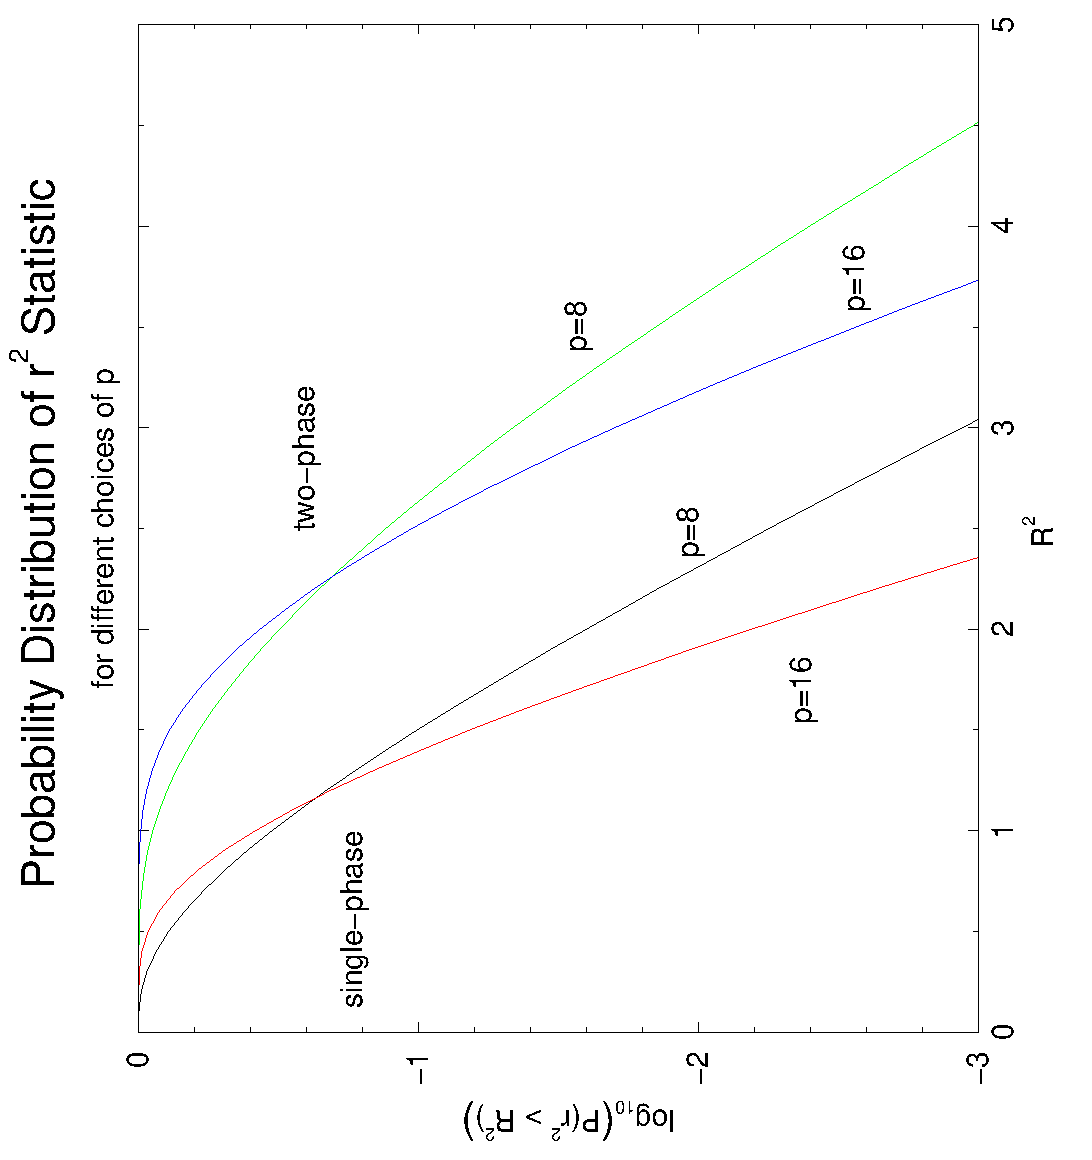
\epsfig{file=Figures/rsquared.eps,angle=-90,width=4in}
\index{colorpage}
\caption{ \label{f:rsquared}
The probability that the $r^2$ statistic exceeds a given threshold $R^2$
is shown for both the single-phase and two-phase test, for $p=8$ and
$p=16$ frequency ranges.  For example, for the single-phase $p=8$ test,
the probability that $r^2 > 2.31$ is 1\% for a chirp plus Gaussian noise.
For the single-phase test with $p=16$ the probability of exceeding the
same threshold is about $10^{-3}$.
}
\end{center}
\end{figure}

\clearpage

\subsection{ How does the $r^2$ test work ?}
In Section \ref{ss:veto} we have derived the statistical properties of
the $r^2$ test, and described it in mathematical terms.  This is a
bit deceptive, because this test was actually developed based on some
simple physical intuition.  We noticed with experience that many of the
high SNR events that were not found by the outlier {\tt is\_gaussian()}
test did not sound anything like chirps (when listened to with the {\tt
audio()} and {\tt sound()} functions).  It was clear from just listening
that for these spurious signals did not have the low frequency signal
arriving first, followed by the high frequency signal arriving last,
in the same way as a chirp signal.  So in fact the $r^2$ test was
designed to discriminate the way in which the different frequencies
arrived with time.  In effect, the filter used to construct the signal
$S_1$ passes only the lowest frequencies, the filter used to construct
the signal $S_2$ passes the next-to-lowest frequencies, and so on.
The filter which produces the signal $S_p$ passes the highest range of
frequencies which would make a significant contribution (i.e. a fraction
$1/p$) of the SNR for a true chirp.

If the signal is a true chirp, then the outputs of each of these different
filters (the $S_i(t_0)$ may be thought of as functions of lag $t_0$)
all peak at the same time-offset $t_0$, the {\it same} time-offset that
maximizes the total signal $S(t_0)$.  This is illustrated in Figure \ref{f:timefreqplot}.
\begin{figure}[h]
\begin{center}
\epsfig{file=Figures/filter3.eps,width=4in,angle=-90}
\index{colorpage}
\caption{
\label{f:timefreqplot}
This figure shows the output of four single-phase filters for the $p=4$
case, for a ``true chirp" injected into a stream of real IFO data
(left set of figures) and a transient noise burst already present in
another stream of real IFO data (right set of figures). When a true
chirp is present, the filters in the different frequency bands all peak
at the same time offset $t_0$: the time offset which maximizes the SNR.
At this instant in time, all of the $S_i$ are about the same value.
However when the filter was triggered by a non-chirp signal, the filters
in the different frequency bands peak at different times, and in fact
at time $t_0$ they have very different values (some large, some small,
and so on).
}
\end{center}
\end{figure}
It is also instructive to compare the values of the filter
outputs (single-phase test) for the two cases shown in Figure
\ref{f:timefreqplot}.  For the injected chirp, the signal-to-noise ratio
was 9.2, and the signal values in the different bands were
\begin{eqnarray}
\nonumber
S_1 & = & 2.25\\
\nonumber
S_2 & = & 2.44\\
\nonumber
S_3 & = & 1.87\\
\nonumber
S_4 & = & 2.64\\
S & = & S_1 + S_2 + S_3 + S_4 = 9.2 \\
\nonumber
r^2 & = & \sum_{i=1}^4 (S/4 - S_i)^2 = 0.324\\
\nonumber
P & = & Q(3/2, 2 r^2) = 0.730,
\end{eqnarray}
so there is a large probability $P$ of having $r^2$ this large.

For the spurious noise event shown in Figure \ref{f:timefreqplot} the
SNR was quite similar (8.97) but the value of $r^2$ is very different:
\begin{eqnarray}
\nonumber
S_1 & = & 0.23\\
\nonumber
S_2 & = & 0.84\\
\nonumber
S_3 & = & 5.57\\
\nonumber
S_4 & = & 2.33\\
S & = & S_1 + S_2 + S_3 + S_4 = 8.97\\
\nonumber
r^2 & = & \sum_{i=1}^4 (S/4 - S_i)^2 = 17.1\\
\nonumber
P & = & Q(3/2, 2 r^2) =9.4 \times 10^{-15},
\end{eqnarray}
so the probability that this value of $r^2$ would be obtained for a chirp
plus Gaussian noise is extremely small.
\clearpage

\subsection{Function: {\tt splitup()}}
\label{ss:splitup}
\setcounter{equation}0
{\tt void splitup(float *working, float template, float *r, int n, float total, int p, int *indices)}\\
This routine takes as inputs a template and a noise-power spectrum, and
splits up the frequency spectrum into a set of sub-intervals to use
with the vetoing technique just described.

The arguments are:
\begin{description}
\item{\tt working:} Input.  An array {\tt working[0..n-1]} used for working space.
\item{\tt template:} Input.  The array {\tt template[0..n-1]} contains the positive
  frequency ($f \ge 0$) part of the complex function $\tilde T(f)$.
  The packing of $\tilde T$ into this array follows the scheme used by
  the {\it Numerical Recipes} routine {\tt realft()}, which is
  described between equations (12.3.5) and (12.3.6) of \cite{NumRec}.
  The DC component $\tilde T(0)$ is real, and located in {\tt template[0]}.
  The Nyquist-frequency component $\tilde T(f_{\rm Nyquist})$ is also
  real, and is located in {\tt template[1]}.  The array elements {\tt template[2]}
  and {\tt template[3]} contain the real and imaginary parts, respectively, of
  $\tilde T(\Delta f)$ where $\Delta f = 2 f_{\rm Nyquist}/n = (n
  \Delta t)^{-1}$.   Array elements {\tt template[2j]} and {\tt template[2j+1]}
  contain the real and imaginary parts of $\tilde T( j \; \Delta f)$
  for $j=1,\cdots,n/2-1$. 
\item{\tt r}: Input.  The array {\tt r[0..n/2]} contains the values of
  the real function $\tilde r$ which is twice the inverse of the receiver noise, as
  in equation (\ref{e:lag}), so that $\tilde r(f) = 2/\tilde
  S_h(|f|)$.  The array elements are arranged in order of increasing
  frequency, from the DC value at subscript 0, to the Nyquist frequency
  at subscript n/2.  Thus, the $j$'th array element {\tt r[j]} contains
  the real value $\tilde r(j \; \Delta f)$, for $j=0,1,\cdots,n/2$.
  Again it is assumed that $\tilde r(-f) = \tilde r^*(f) = \tilde r(f)$.
\item{\tt n}: Input.  The total length of the complex arrays
  {\tt template} and {\tt working}, and the number of points in the output
  array {\tt s}.  Note that the array {\tt r} contains $n/2+1$
  points.  n must be even.
\item{\tt total:} Input.  This is the total value of the integrated
  template squared over $S_h$; the frequency
  subintervals are choose so that each of the {\tt p} subintervals
  contains $1/p$ of this total.
\item{\tt p:} Input.  The number of frequency bands into which you want to divide the range
  from DC to $f_{\rm Nyquist}$.
\item{\tt indices:} Ouput.  The frequency bins of the first frequency band are
  {\tt i=0..indices[0]}.  The next frequency band is  {\tt i=indices[0]+1..indices[1]}.
  The {\tt p}'th frequency band is {\tt i=indices[p-2]+1..indices[p-1]}.
  Note that {\tt indices[p-1]=n-1}.
\end{description}
\begin{description}
\item{Author:}
Bruce Allen, ballen@dirac.phys.uwm.edu
\item{Comments:}
None.
\end{description}
\clearpage

\subsection{Function: {\tt splitup\_freq()}}
\label{ss:splitup_freq}
\setcounter{equation}0
{\tt float splitup\_freq(float c0, float c90, float *chirp0,  float
*chirp90, float norm, float* twice\_inv\_noise, int n, int offset, int
p, int* indices, float* stats, float* working, float* htilde)}\\
This routine returns the value of the statistic $r^2=\sum_{i=1}^p (\Delta S_i)^2$.  This is
a less-efficient version, which internally constructs filters for each of the different frequency
subintervals, and then filters the metric perturbation through those filters.  It is useful
to understand how the different frequency components behave in the time domain, after filtering.

The arguments are:
\begin{description}
\item{\tt c0:} Input.  The coefficient of the 0-phase template.
\item{\tt c90:} Input.  The coefficient of the $90^\circ$-phase template.  Note that
    $c_0^2 + c_{90}^2$ should be 1.
\item{\tt chirp0:} Input.  An array {\tt chirp0[0..n-1]} containing the FFT of the 0-phase chirp.
\item{\tt chirp90:} Input.  An array {\tt chirp90[0..n-1]} containing the FFT of the $90^\circ$-phase chirp.
\item{\tt norm:} Input.  The normalization of the 0-phase chirp.
\item{\tt twice\_inv\_noise:} Input.  The array {\tt twice\_inv\_noise[0..n/2]} contains $2/S_h(f)$,
   as described previously.
The array element {\tt twice\_inv\_noise[0]} contains
   the DC value, and the array element {\tt twice\_inv\_noise[n/2]}
   contains the value at the Nyquist frequency.
\item{\tt n:} Input.  Defines the lengths of the previous arrays.
\item{\tt offset:} Input.  The offset of the moment of maximum signal in the filter output.
\item{\tt p:} Input.  The number of frequency bands $p$ for the vetoing test.
\item{\tt indices:} Output.  An array {\tt indices[0..p-1]} used for internal storage of the
   frequency subintervals (see {\tt splitup()}.
\item{\tt stats:} Output.  An array {\tt stats[0..p-1]} containing the values of the $S_i$ for $i=1,\cdots,p$.
\item{\tt working:} Output.  An array {\tt working[0..n-1]} used for internal storage.
\item{\tt htilde:} Input.  An array {\tt htilde[0..n-1]} containing the positive frequency part of
  $\tilde h(f)$.
\end{description}
\begin{description}
\item{Author:}
Bruce Allen, ballen@dirac.phys.uwm.edu
\item{Comments:}
None.
\end{description}
\clearpage

\subsection{Function: {\tt splitup\_freq2()}}
\label{ss:splitup_freq2}
\setcounter{equation}0
{\tt float splitup\_freq2(float c0, float c90, float *chirp0,  float
*chirp90, float norm, float* twice\_inv\_noise, int n, int offset, int
p, int* indices, float* stats, float* working,float* htilde)}\\
This routine returns the value of the statistic $r^2=\sum_{i=1}^p
(\Delta S_i)^2$.  This is a more computationally-efficient version,
which does not filter $\tilde h$ through each of the $p$ independent
time domain filters.  The arguments are identical to those of {\tt splitup\_freq()}.

The arguments are:
\begin{description}
\item{\tt c0:} Input.  The coefficient of the 0-phase template.
\item{\tt c90:} Input.  The coefficient of the $90^\circ$-phase template.  Note that
    $c_0^2 + c_{90}^2$ should be 1.
\item{\tt chirp0:} Input.  An array {\tt chirp0[0..n-1]} containing the FFT of the 0-phase chirp.
\item{\tt chirp90:} Input.  An array {\tt chirp90[0..n-1]}
containing the FFT of the $90^\circ$-phase chirp.
\item{\tt norm:} Input.  The normalization of the 0-phase chirp.
\item{\tt twice\_inv\_noise:} Input.  The array {\tt twice\_inv\_noise[0..n/2]} contains $2/S_h(f)$,
   as described previously.
The array element {\tt twice\_inv\_noise[0]} contains
   the DC value, and the array element {\tt twice\_inv\_noise[n/2]}
   contains the value at the Nyquist frequency.
\item{\tt n:} Input.  Defines the lengths of the previous arrays.
\item{\tt offset:} Input.  The offset of the moment of maximum signal in the filter output.
\item{\tt p:} Input.  The number of frequency bands $p$ for the vetoing test.
\item{\tt indices:} Output.  An array {\tt indices[0..p-1]} used for internal storage of the
   frequency subintervals (see {\tt splitup()}.
\item{\tt stats:} Output.  An array {\tt stats[0..p-1]} containing the values of the $S_i$ for $i=1,\cdots,p$.
\item{\tt working:} Output.  An array {\tt working[0..n-1]} used for internal storage.
\item{\tt htilde:} Input.  An array {\tt htilde[0..n-1]} containing the positive frequency part of
  $\tilde h(f)$.
\end{description}
\begin{description}
\item{Author:}
Bruce Allen, ballen@dirac.phys.uwm.edu
\item{Comments:}
None.
\end{description}
\clearpage


\subsection{Function: {\tt splitup\_freq3()}}
\setcounter{equation}0
{\tt float splitup\_freq2(float c0, float c90, float *chirp0, float
*chirp90, float norm, float* twice\_inv\_noise, int n, int offset, int p,
int* indices, float* stats, float* working,float* htilde)}\\
This routine implements the two-phase $r^2$ statistic test.  It returns
the value of the statistic $r^2=\sum_{i=1}^p |\Delta S_i|^2$ as defined
in Eq.~(\ref{e:deftwhophaser2}).  It is algorithmically similar to {\tt
splitup\_freq2()},  except that it allows for the case where the phase
of the signal is unknown.  The arguments are identical to those of {\tt
splitup\_freq2()} but the array {\tt stats} has $2p$ elements since the
signals are complex.

Note: The GRASP library includes two additional functions which are
operationally identical to {\tt splitup\_freq3()}, called
{\tt splitup\_freq4()} and {\tt splitup\_freq5()}.  The last of
these is currently the most efficient implementation of the two-phase
$r^2$ test.  All the arguments of {\tt splitup\_freq[3-5]()} are
{\it identical}.

The arguments are:
\begin{description}
\item{\tt c0:} Input.  Used in the same way as in {\tt splitup\_freq2()}. 
\item{\tt c90:} Input.  Used in the same way as in {\tt splitup\_freq2()}.  Note that
 if templates have unit norm you can set $c_0^2 + c_1^2 = 4$.
\item{\tt chirp0:} Input.  An array {\tt chirp0[0..n-1]} containing 
the FFT of the 0-phase chirp.
\item{\tt chirp90:} Input.  An array {\tt chirp90[0..n-1]}
containing the FFT of the $90^\circ$-phase chirp.
\item{\tt norm:} Input.  The normalization of the 0-phase chirp.
\item{\tt twice\_inv\_noise:} Input.  The array {\tt
twice\_inv\_noise[0..n/2]} contains $2/S_h(f)$, as described previously.
The array element {\tt twice\_inv\_noise[0]} contains the DC value,
and the array element {\tt twice\_inv\_noise[n/2]} contains the value 
at the Nyquist frequency.
\item{\tt n:} Input.  Defines the lengths of the previous arrays.
\item{\tt offset:} Input.  The offset of the moment of maximum signal 
in the filter output.
\item{\tt p:} Input.  The number of frequency bands $p$ for the vetoing test.
\item{\tt indices:} Output.  An array {\tt indices[0..p-1]} used for
internal storage of the frequency subintervals (see {\tt splitup()}.
\item{\tt stats:} Output.  An array {\tt stats[0..2p-1]} containing
the real and imaginary parts of the $S_i$ for $i=1,\cdots,p$.
\item{\tt working:} Output.  An array {\tt working[0..n-1]} used for 
internal storage.
\item{\tt htilde:} Input.  An array {\tt htilde[0..n-1]} containing 
the positive frequency part of $\tilde h(f)$.
\end{description}
\begin{description}
\item{Authors}
Bruce Allen, ballen@dirac.phys.uwm.edu,
and Patrick Brady,  patrick@tapir.caltech.edu,
and Jolien Creighton jolien@tapir.caltech.edu.
\item{Comments:}
None.
\end{description}
\clearpage

\subsection{Example: {\tt optimal} program}
\setcounter{equation}0
This program reads the 40-meter data stream, and then filters it though
a chirp template corresponding to a pair of inspiraling $1.4 M_\odot$
neutron stars.

The correspondence between different arrays in this program, and the
quantities discussed previously in this section, is given below.  In these
equations, $\Delta t = 1/{\tt srate}$ is the sample time in seconds, and
$\Delta f = (n \Delta t)^{-1} = {\tt srate/npoint}$ is the size of a
frequency bin, in Hz.  Here $n={\tt npoint}$ is the number of points in
the data stream which are being optimally filtered in one pass.

Chirp templates (in frequency space) for the two polarizations are
related to the arrays \hbox{\tt chirp0[ ]} and \hbox{\tt chirp1[ ]} by
\begin{eqnarray}
\tilde T_{0}(f) &=& {\Delta t  \over {\tt HSCALE}} \;{\tt chirp0[\;]}\\
\tilde T_{90}(f) &=& {\Delta t \over {\tt HSCALE}} \; {\tt chirp1[\;]}
\end{eqnarray}
where the elements {\tt chirp0[2j]} and {\tt chirp0[2j+1]} are the real
and imaginary parts at frequency $f= j \Delta f$ (with the exception of
the Nyquist frequency, stored in {\tt chirp0[1]}).  Note that to ensure
that quantities within the code remain within the dynamic range of
floating point numbers, we have scaled up the template strain by a
constant factor {\tt HSCALE}; we also scale up the interferometer
output by the same factor, so that all program output (such as
signal-to-noise ratios) is independent of the value of {\tt HSCALE}.
If you're not comfortable with this, go ahead and change {\tt HSCALE} to 1.
It won't change anything, provided that you don't overflow the dynamic
range of the floating point variables!
The scaled interferometer response function is
\begin{equation}
{\tt response[\;]} = {\tt HSCALE}/{\tt ARMLENGTH} \times R(f),
\end{equation}
where the function $R(f)$ is defined by equation (\ref{e:rdef}).
The Fourier transform $\tilde h$ of the dimensionless strain is
obtained by multiplying $\Delta t$ and the FFT of {\tt channel.0} by
{\tt response[ ]}, yielding
\begin{equation}
\tilde h(f) = {\Delta t \over {\tt HSCALE}} {\tt htilde[\;]}.
\end{equation}
The one-sided noise power spectrum $S_h(f)$ is the average of 
\begin{equation}
S_h(f) = {2 \over n \Delta t} | \tilde h(f) |^2 =
{2 \over n \Delta t} {(\Delta t)^2 \over {\tt HSCALE}^2} |{\tt htilde[\;]}|^2
= {2 \Delta t \over n \; {\tt HSCALE}^2} |{\tt htilde[\;]}|^2.
\end{equation}
The power spectrum $S_h(f)$ is averaged using the same exponential
averaging technique described for the routine {\tt avg\_spec()}.  This
average is stored as
\begin{equation}
{  S_h(f)} = {2 \Delta t \over n \; {\tt HSCALE}^2 }
\langle |{\tt htilde[\;]}|^{2} \rangle 
= { \Delta t \over n \; {\tt HSCALE}^2 } {\tt mean\_pow\_spec[\;]}
\end{equation}
Twice the inverse of this average is stored in the array {\tt
twice\_inv\_noise[ ]}, so that
\begin{equation}
{2 \over S_h(f)} = { n \; {\tt HSCALE}^2 \over \Delta t} \; {\tt twice\_inv\_noise[\;]}.
\end{equation}
The expected noise-squared for the plus polarization is given by
equation (\ref{e:n2}):
\begin{eqnarray*}
\langle N^2 \rangle &=& {1 \over 2} (Q,Q)  = {1 \over 2} \int_{-\infty}^\infty df\;
{| \tilde T_{0}(f)|^2 \over S_h(f)} \\
&=&
{1 \over 2} {1 \over n \Delta t} FFT^{-1}_0 \left[
 {(\Delta t)^2 \over {\tt HSCALE}^2}  |{\tt chirp0[\;]} |^2 
{n {\tt HSCALE}^2 \over \Delta t} {1 \over 2} {\tt twice\_inv\_noise[\; ] } \right] \\
& = & {1 \over 2} FFT^{-1}_0 \left[ |{\tt chirp0[\;]} |^2 {1 \over 2} {\tt twice\_inv\_noise[\; ] } \right] \\
& \rightarrow & {1 \over 2} {\tt
correlate(\cdots,chirp0[\;],chirp0[\;],twice\_inv\_noise[\;],npoint)}.
\end{eqnarray*}
where the subscript on the inverse FFT means ``at zero lag", and
``$\rightarrow f$" means ``returned by the call to the function f".  We
have chosen a distance for the system producing the ``chirp" $\tilde
T_(f)$ so that the expected value of $\langle N^2 \rangle=1$.

In similar fashion, the signal $S$ at lag $t_0 $ is given
by
\begin{eqnarray}
   \nonumber
S  & = & ({\tilde h \over S_h}, \tilde Q) \\
    \nonumber
    & = & \int_{-\infty}^\infty df\;
       {\tilde h(f) \tilde T^*_{0}(f)  \over S_h(f)} \;
       {\rm e}^{-2 \pi i f t_0} \\
   \nonumber
   & = & {1 \over n \Delta t} FFT^{-1}_{i}\left[ {\Delta t \over {\tt
       HSCALE}} {\tt htilde[\;]} {\Delta t  \over {\tt HSCALE}} \;
       \left( {\tt chirp0[\;]} \right)^* { n \; {\tt HSCALE}^2 \over
       \Delta t } \; {1 \over 2} {\tt twice\_inv\_noise[\;]} \right] \\
\nonumber
   & = & FFT^{-1}_{i} \left[ {\tt htilde[\;]} \; {\tt chirp0[\;]} \;
   {1 \over 2} {\tt twice\_inv\_noise[\;]} \right]\\
& \rightarrow & {\tt
correlate(\cdots,htilde[\;],chirp0[\;],twice\_inv\_noise[\;],npoint)},
\end{eqnarray}
where now the subscript on the FFT means ``at lag $t = i \; \Delta t$".

You might wonder why we have been so careful -- after all, both the
signal and the noise, as we've defined them, are dimensionless, so it's
not surprising that all of the factors of $\Delta t$ drop out of the
final formulae for the signal and the expected noise-squared.  The main
reason we've been so long winded is to show exactly how the units cancel out,
and to demonstrate that there aren't any missing dimensionless constants,
like {\tt npoint}, left out of the program.  Some sample output from
this program is shown in the next section.
\clearpage
\lgrindfile{Includes/optimal.tex}
\clearpage

\subsection{Some output from the {\tt optimal} program}
Some output from the {\tt optimal} program follows:
\begin{verbatim}
...
max snr: 3.11 offset: 23623 data start: 180.00 sec. variance: 0.94044
max snr: 2.91 offset: 3311 data start: 185.17 sec. variance: 0.84484
...
max snr: 2.53 offset: 19041 data start: 309.26 sec. variance: 0.70333
max snr: 2.98 offset: 35711 data start: 314.43 sec. variance: 0.67523

Max SNR: 8.71 (offset 42109) variance 0.805030
   If impulsive event, offset 55624 or time 325.23
   If inspiral, template start offset 42109 (time 323.86) coalescence time 325.23
   Normalization: S/N=1 at 116.75 kpc
   Linear combination of max SNR: 0.9315 x phase_0 + 0.3638 x phase_pi/2
   Less than 1% probability that this is a chirp (p=0.000000).
   Distribution: s= 23, N>3s= 12 (expect 176), N>5s= 0 (expect 0)
   Distribution does not appear to have outliers...

max snr: 2.51 offset: 31183 data start: 324.77 sec. variance: 0.63028
max snr: 2.56 offset: 49909 data start: 329.94 sec. variance: 0.66853
...
max snr: 2.82 offset: 35080 data start: 3002.03 sec. variance: 0.77306
max snr: 2.61 offset: 33141 data start: 3007.20 sec. variance: 0.74268

Max SNR: 89.75 (offset 16678) variance 82.547005
   If impulsive event, offset 30193 or time 3015.43
   If inspiral, template start offset 16678 (time 3014.06) coalescence time 3015.43
   Normalization: S/N=1 at 128.49 kpc
   Linear combination of max SNR: -0.3955 x phase_0 + 0.9185 x phase_pi/2
   Less than 1% probability that this is a chirp (p=0.000000).
   Distribution: s= 29, N>3s= 157 (expect 176), N>5s= 30 (expect 0)
   Distribution has outliers! Reject

max snr: 3.24 offset: 22412 data start: 3017.54 sec. variance: 0.99474
max snr: 2.73 offset: 37777 data start: 3022.71 sec. variance: 0.75325
...
max snr: 2.80 offset: 5893 data start: 4140.89 sec. variance: 0.73240
max snr: 2.75 offset: 46932 data start: 4146.06 sec. variance: 0.69654

Max SNR: 6.08 (offset 30002) variance 0.883380
   If impulsive event, offset 43517 or time 4155.64
   If inspiral, template start offset 30002 (time 4154.27) coalescence time 4155.64
   Normalization: S/N=1 at 113.04 kpc
   Linear combination of max SNR: -0.4773 x phase_0 + 0.8787 x phase_pi/2
   POSSIBLE CHIRP!  with > 1% probability (p=0.024142).
   Distribution: s= 31, N>3s= 399 (expect 176), N>5s= 53 (expect 0)
   Distribution has outliers! Reject

max snr: 2.77 offset: 15985 data start: 4156.40 sec. variance: 0.72095
max snr: 2.69 offset: 47338 data start: 4161.57 sec. variance: 0.69708
...
\end{verbatim}
This output shows three events that triggered an optimal filtering
routine.  The first and second of these events were rejected for
different reasons.  The first was rejected because if failed the
frequency-distribution test.  The second was rejected because it had 30
outlier points.  The third failed for the same reason: it had 53
outlier points.

Next, we show some output when a fake chirp signal is injected into the data stream.  This
can be done for example by modifying {\tt optimal} to read:
\begin{verbatim}
invMpc_inject=100.0;   /* To inject a signal at 10 kpc, set this to 100.0 */
time_inject_chirp(1.0,0.0,12345,invMpc_inject,chirp0,chirp90,data,response,output0,npoint);
\end{verbatim}
This produces the following output:
\begin{verbatim}
...
Max SNR: 9.96 (offset 12345) variance 0.872624
   If impulsive event, offset 25860 or time 187.79
   If inspiral, template start offset 12345 (time 186.42) coalescence time 187.79
   Normalization: S/N=1 at 152.17 kpc
   Linear combination of max SNR: 0.9995 x phase_0 + -0.0304 x phase_pi/2
   POSSIBLE CHIRP!  with > 1% probability (p=0.421294).
   Distribution: s= 23, N>3s= 12 (expect 176), N>5s= 0 (expect 0)
   Distribution does not appear to have outliers...


Max SNR: 12.84 (offset 12345) variance 0.834527
   If impulsive event, offset 25860 or time 192.96
   If inspiral, template start offset 12345 (time 191.59) coalescence time 192.96
   Normalization: S/N=1 at 132.47 kpc
   Linear combination of max SNR: 0.9953 x phase_0 + 0.0973 x phase_pi/2
   POSSIBLE CHIRP!  with > 1% probability (p=0.949737).
   Distribution: s= 22, N>3s= 28 (expect 176), N>5s= 0 (expect 0)
   Distribution does not appear to have outliers...


Max SNR: 14.86 (offset 12345) variance 0.801640
   If impulsive event, offset 25860 or time 198.13
   If inspiral, template start offset 12345 (time 196.76) coalescence time 198.13
   Normalization: S/N=1 at 127.90 kpc
   Linear combination of max SNR: 0.9993 x phase_0 + -0.0372 x phase_pi/2
   POSSIBLE CHIRP!  with > 1% probability (p=0.999236).
   Distribution: s= 22, N>3s= 35 (expect 176), N>5s= 0 (expect 0)
   Distribution does not appear to have outliers...
...
\end{verbatim}
The code is correctly finding the chirps, getting the distance and phase and
time location of the chirps about as accurately as one would expect given
the level of the IFO noise.

There are several interesting lessons that one can learn from this
optimal filtering experience.  The first is that (roughly speaking) the
events that trigger an optimal filter (driving the output to a value
much larger than would be expected for a colored-noise Gaussian input)
can be broken into two classes: those which can be seen in the raw data
stream, and those which can not.  Here, by ``seen in the raw data
stream", we mean ``visible to the naked eye upon examination of a
graph".  Shown in the following two figures are examples of each type
of spurious event.

\begin{figure}
\begin{center}
\epsfig{file=Figures/data.000.ps,angle=-90,bbllx=40pt,bblly=72pt,
bburx=580pt,bbury=720pt,width=4in}
\index{colorpage}
\caption{ \label{f:drip}
This shows the event that triggered the $2\times 1.4$ solar mass binary
inspiral filter with a SNR of 8.71 (see the first set of sample output
from the optimal filtering code above, at time 325.23).  This same
``event" can also be seen in Figure~\ref{f:diag0}.  The horizontal axis
is sample number, with samples $\approx 10^{-4}$ seconds apart; the
vertical axis is the raw (whitened) IFO output.  The event labeled
``drip" can be heard in the data (it sounds like a faucet drip) and is
picked up by the optimal filtering technique, but it is NOT visible to
the naked eye.  This event is vetoed by the splitup technique described
earlier - it has extremely low probability of being a chirp plus
stationary noise.}
\end{center}
\end{figure}

\begin{figure}
\begin{center}
\epsfig{file=Figures/data.001.ps,angle=-90,bbllx=40pt,bblly=72pt,
bburx=580pt,bbury=720pt,width=4in}
\index{colorpage}
\caption{ \label{f:bump1}
This another event that triggered the $2\times 1.4$ solar mass binary
inspiral filter with a SNR of 17.33.  This event sounds like a ``bump";
it is probably due to a bad cable connection.  It can be easily seen
(and vetoed) in the time domain.  A close-up of this is shown in the next
figure.}
\end{center}
\end{figure}

\begin{figure}
\begin{center}
\epsfig{file=Figures/data.001b.ps,angle=-90,bbllx=40pt,bblly=72pt,
bburx=580pt,bbury=720pt,width=4in}
\index{colorpage}
\caption{ \label{f:bump2}
A close-up of the previous graph, showing the structure of the ``bump".}
\end{center}
\end{figure}

\begin{figure}
\begin{center}
\epsfig{file=Figures/data.002.ps,angle=-90,bbllx=40pt,bblly=72pt,
bburx=580pt,bbury=720pt,width=4in}
\caption{ \label{f:scrape1}
This another event that triggered the $2\times 1.4$ solar mass binary
inspiral filter with a SNR of 32.77.  This event sounds like a shovel
scraping on the ground; its origin is unknown.  It can be easily seen
(and vetoed) in the time domain.}
\end{center}
\index{colorpage}
\end{figure}

\begin{figure}
\begin{center}
\epsfig{file=Figures/data.002b.ps,angle=-90,bbllx=40pt,bblly=72pt,
bburx=580pt,bbury=720pt,width=4in}
\caption{ \label{f:scrape2}
A close-up of the previous graph, showing the structure of the ``scrape".}
\end{center}
\end{figure}
\index{colorpage}
\clearpage

\clearpage
\subsection{The effective distance to which a source can be seen}
\label{ss:eff_distdef}
\par\noindent

Given a gravitational-wave detector with some known noise spectrum, it
would clearly be useful to define an ``effective distance'' $D_{\rm
eff}$ to which some given gravitational-wave source can be seen.  To
first order, any source located farther away from the detector than
$D_{\rm eff}$ would be too weak to be detectable in the datastream.
Sources closer than $D_{\rm eff}$ would be detectable.

This naive, heuristic picture of $D_{\rm eff}$ doesn't make much sense
in the real world because the source does not emit isotropically, and
the detector does not detect isotropically: there are positions on the
sky for which the detector can ``see'' farther, and the source
radiates more strongly into some angles than others.  A useful
definition of $D_{\rm eff}$ must therefore average over angles in a
meaningful, well-understood way.

One simple way to average over angles is to use Eq. (2.30) of Ref.\
{\cite{flanhughes1}}.  In that reference, Flanagan and Hughes show
that the signal-to-noise ratio, rms angle averaged over all source
orientations and all positions on the sky, depends only on the
spectrum of emitted gravitational-wave energy, $dE_{\rm gw}/df$.
Rearranging their formula (2.30) slightly, the effective distance to
which a source can be seen with some rms angle-averaged
signal-to-noise ratio $\rho_0$ is then
\begin{equation}
D^{\rm FH}_{\rm eff}(\rho_0)^2 = 
 {2(1+z)^2\over5\pi^2\rho_0^2}
\left( {G \over c^3} \right) \int_0^\infty df {1\over f^2 S_h(f)}{dE_{\rm gw}\over df}[(1+z)f]\;.
\label{eq:effdist_fh}
\end{equation}
The distance $D^{\rm FH}_{\rm eff}$ so defined is actually a
luminosity distance; assuming some set of cosmological parameters and
using standard formulae, one can then easily convert $D^{\rm FH}_{\rm
eff}$ to an effective redshift $z^{\rm FH}_{\rm eff}$, and thence
compute the comoving volume $V_c(z^{\rm FH}_{\rm eff})$ that is
contained to that distance.  If one assumes that the event rate of
sources locked into Hubble flow does not evolve with redshift, this
allows one to simply convert from an event rate density $R$ [with
units number/(Mpc$^3$ year)] to a detected event rate $N$ (with units
number/year).  (This assumption is clearly a rather bad one: the event
rate will undoubtedly evolve with redshift.  However, we don't
currently know {\it how} it will so evolve.  This simple, albeit
stupid, assumption is a useful one for estimating event rates for
gravitational-wave sources.)

Notice that the cosmological redshift $z$ explicitly appears in
Eq. (\ref{eq:effdist_fh}).  These factors enter in such a way that the
mass ``imprinted'' on the gravitational waveform ({\it i.e.}, the mass
that gravitational-wave detections measure at the earth) will be
redshift from $M$ to $(1+z)M$.

Finn and Chernoff {\cite{finnandchernoff}} define an effective
distance in a somewhat different and more careful manner.
Given a noise spectrum and given a threshold signal-to-noise ratio
$\rho_0$, they define an effective distance $D^{\rm FC}_{\rm
eff}(\rho_0)$ as
\begin{equation}
N(\rho > \rho_0)  = {4\pi\over3} D^{\rm FC}_{\rm eff}(\rho_0)^3 R\;.
\label{eq:effdist_fc}
\end{equation}
In words, the detection rate of events with signal-to-noise ratio
$\rho$ greater than the threshold $\rho_0$ is given the event rate
density in space $R$ times the volume of a sphere of radius $D^{\rm
FC}_{\rm eff}(\rho_0)$.  Finn and Chernoff then calculate $D^{\rm
FC}_{\rm eff}$ using Monte-Carlo integration; see
{\cite{finnandchernoff}} for details.

Thorne {\cite{thornetofinnhughes},\cite{thornefinnerror}} has shown
that for a pair of $1.4\,M_\odot-1.4\,M_\odot$ neutron stars {\it and}
for distances small enough that cosmological effects are negligible,
the definitions given in Eqs.\ (\ref{eq:effdist_fh}) and
(\ref{eq:effdist_fc}) are related by
\begin{equation}
{D^{\rm FC}_{\rm eff}\over D^{\rm FH}_{\rm eff}} = 1.10\;.
\label{eq:fudgefactor}
\end{equation}
For the purposes of GRASP, we will use an effective distance that is
based on (\ref{eq:effdist_fh}) because it is quick and simple to
calculate, but correct using (\ref{eq:fudgefactor}) in the hope that
this will put us in reasonable agreement with the very careful
calculations of Finn and Chernoff.  (This factor of $1.10$ probably
varies somewhat with total system mass and with cosmological effects.)
The formula for $D_{\rm eff}(\rho_0)$ that we use is
\begin{equation}
D_{\rm eff}(\rho_0)^2 = (1.10)^2 \times{2(1+z)^2\over5\pi^2
\rho_0^2}\int_0^\infty df {1\over f^2 S_h(f)}{dE_{\rm gw}
\over df}[(1+z)f]\;.
\label{eq:effdist}
\end{equation}

The following routine calculates this effective distance, providing
also the associated redshift and comoving volume.

\clearpage
\subsection{Function: {\tt inspiral\_dist()}}
\label{ss:inspiral_dist}
\begin{verbatim}
void inspiral_dist(double *deff, double *z, double *Vc, double m1_z,
                   double m2_z, double snr, double S_h[], int npoint,
                   double srate, double h100)
\end{verbatim}
\noindent
This function computes the effective distance to which a binary
inspiral with redshifted masses {\tt m1\_z} and {\tt m2\_z} can be
seen with the noise spectrum {\tt S\_h[]}.

It uses the energy spectrum
\begin{equation}
{dE_{\rm gw}\over df} = {\pi^{2/3} \over 3}\mu M^{2/3} f^{-1/3}
\label{eq:inspspec}
\end{equation}
to describe the inspiral for frequencies $f < f_{\rm merge} = 0.02/M$,
and zero above $f_{\rm merge}$ (as in reference {\cite{flanhughes1}}).
To convert from luminosity distance to redshift, it assumes a universe
flat cosmology ($\Lambda=0$, $\Omega=1$) with a Hubble constant $H_0 =
75\,{\rm km}/{{\rm Mpc}\,{\rm sec}}$, and uses an Eq. (11) from
{\cite{markovic}}.  To convert from redshift to comoving volume, it
uses Eq. (27) of {\cite{dwhogg}} or Eq. (2.56) with $q_0=1/2$ of
\cite{kolbturner}.

The arguments to the function are:
\begin{description}
\item{{\tt deff:}} Output.  The effective distance in megaparsecs.
\item{{\tt z:}} Output.  Redshift corresponding that effective distance.
\item{{\tt Vc:}} Output.  Comoving volume at the redshift in cubic
megaparsecs.
\item{{\tt m1\_z:}} Input.  Redshifted mass one, $(1+z)m_1$.
\item{{\tt m2\_z:}} Input.  Redshifted mass two, $(1+z)m_2$.
\item{{\tt snr:}} Input.  The signal-to-noise ratio at which the
effective distance is {\tt deff}.
\item{{\tt S\_h:}} Input.  The spectral density of noise in Hz$^{-1}$.
\item{{\tt npoint:}} Input.  The number of data points in {\tt S\_h}.
\item{{\tt srate:}} Input.  The sampling rate used to construct the
noise spectrum, Hz.
\item{{\tt h100:}} Input.  The Hubble constant in units of 100 km/sec/Mpc.
\end{description}

\begin{description}
\item{Author:} Scott Hughes, hughes@tapir.caltech.edu
\end{description}
     
\clearpage
\subsection{Function: {\tt merger\_dist()}}
\label{ss:merger_dist}
\begin{verbatim}
void merger_dist(double *deff, double *z, double *Vc, double m1_z,
                 double m2_z, double snr, double S_h[], int npoint,
                 double srate,double h100)
\end{verbatim}
\noindent
This function computes the effective distance to which a binary
merger with redshifted masses {\tt m1\_z} and {\tt m2\_z} can be
seen with the noise spectrum {\tt S\_h[]}.

It uses the energy spectrum
\begin{equation}
{dE_{\rm gw}\over df} = {\epsilon M\over f_{\rm qnr} - f_{\rm merge}}
\label{eq:mergspec}
\end{equation}
to describe the merger, using parameters $\epsilon = 0.1$, $f_{\rm
qnr} = 0.13/M$, $f_{\rm merge} = 0.02/M$ (as in reference
{\cite{flanhughes1}}).  As such it is, strictly speaking, only
applicable to binary black hole mergers.  Its operation is otherwise
identical to {\tt inspiral\_dist()}.

The arguments to the function are:
\begin{description}
\item{{\tt deff:}} Output.  The effective distance in megaparsecs.
\item{{\tt z:}} Output.  Redshift corresponding that effective distance.
\item{{\tt Vc:}} Output.  Comoving volume at the redshift in cubic
megaparsecs.
\item{{\tt m1\_z:}} Input.  Redshifted mass one, $(1+z)m_1$.
\item{{\tt m2\_z:}} Input.  Redshifted mass two, $(1+z)m_2$.
\item{{\tt snr:}} Input.  The signal-to-noise ratio at which the
effective distance is {\tt deff}.
\item{{\tt S\_h:}} Input.  The spectral density of noise in Hz$^{-1}$.
\item{{\tt npoint:}} Input.  The number of data points in {\tt S\_h}.
\item{{\tt srate:}} Input.  The sampling rate used to construct the
noise spectrum, Hz.
\item{{\tt h100:}} Input.  The Hubble constant in units of 100 km/sec/Mpc.
\end{description}

\begin{description}
\item{Author:} Scott Hughes, hughes@tapir.caltech.edu
\end{description}

\clearpage
\subsection{Example: {\tt compute\_dist} program}
\label{ss:compute_dist}

This program will tell you the distance to which a binary with given
redshifted masses [$(1+z)m_1,(1+z)m_2$] can be seen with a given
signal-to-noise rate in some given detector (which must be listed in
the GRASP file {\tt detectors.dat}).  It will also tell you the
redshift at that effective (luminosity) distance and the corresponding
comoving volume.  It uses that comoving volume to convert a given
event rate density to a measured event rate.

The code specifies its various input parameters with command line
flags.  Thus,\\
{\tt compute\_dist -m1 5 -m2 7 -snr 6 -d 24 -R 2.e-7 -h100 0.75}\\
will compute the effective distance for a binary that has $(1+z)m_1 =
5M_\odot$, $(1+z)m_2 = 7M_\odot$ with signal-to-noise ratio 6 in detector
24 (the zeroth stage of enhancement at the Livingston LIGO site); and it
will compute the detected event rate with an assumption that the event
rate density is $2\times10^{-7}$ events per cubic megaparsec per year,
in a cosmology with Hubble constant today of 75 km/sec/Mpc.  If a flag
or parameter is omitted, default values are used; type\\
{\tt compute\_dist -h}\\
 to see those default
values.
     
\lgrindfile{Includes/compute_dist.tex}

\begin{description}
\item{Author:} Scott Hughes, hughes@tapir.caltech.edu
\end{description}


% GRASP: Copyright 1997,1998,1999  Bruce Allen
% $Id: man_testmass.tex,v 1.5 1999/07/11 21:22:17 ballen Exp $
%
% GRASP Routines: Waveforms from perturbation theory
% Author: S.Droz (droz@physics.uoguelph.ca)
%
%
% $Id: man_testmass.tex,v 1.5 1999/07/11 21:22:17 ballen Exp $
%
% $Log: man_testmass.tex,v $
% Revision 1.5  1999/07/11 21:22:17  ballen
% Added RCS id strings
%
% Revision 1.4  1998/10/05 19:14:54  ballen
% Updated manual to use new hyperref package.
%
% Revision 1.3  1998/06/06 20:43:28  ballen
% Serge modified manuals, and added figure.
%
% Revision 1.5  1998/04/01 22:02:24  droz
% This is the version in GRASP 1.6.5.
%
% Revision 1.3  1998/02/25 21:44:15  droz
% All routines and the error messages are now documented.
% We still need to add the examples and correct all the errors.
%
% Revision 1.2  1998/02/24 22:11:31  droz
% Most routines are now documented.
%
% Revision 1.1  1998/02/23 22:02:10  droz
% Initial revision
%
%
 \DeclareRobustCommand{\nicefrac}[2]{\hspace{0.1em}%
  \raisebox{0.5ex}{${\scriptstyle
#1}$}\hspace{-0.1em}/\hspace{-0.07em}%
  \mbox{${\scriptstyle #2}$}}
\section{GRASP Routines: Waveforms from perturbation theory}
\label{s:BHPT}
\setcounter{equation}0
An alternative method of calculating the waveforms generated during a binary
inspiral is provided by black hole perturbation theory.
In the limit of a small mass ratio $\eta = \nicefrac{m_1 m_2}{(m_1 + m_2)^2}$ (the
test mass limit) we can treat the effects of the smaller body as perturbations of
the gravitational field of the larger mass. If the latter is a black hole then
the Teukolsky formalism \cite{teukolsky:1973} can be used to calculate these perturbations.
The corrections to 
the metric are then expressed as an infinite sum over multipole 
moments. Here we will consider the case of a Schwarzschild black hole.

\subsection{The waveform}

The Teukolsky formalism gives the two components $h_+$ and $h_\times$ of the
gravitational waves produced by a test mass in a fixed, circular orbit of radius $r_0$
 as
\begin{equation}
  h_+(u) - i h_\times(u) = \frac{2 G \mu}{r c^2} \sum_{l\geq 2, |m| \leq l}
            A_{lm}(M \Omega) e^{-i m \Omega (t - c r^*)} {}_{-2}Y_{lm}(\vartheta,
                        \varphi),
        \label{e:wave1}
\end{equation}
where  $u=t-c r^*$ is the standard retarded time. Here $G$ is Newton's constant and
$c$ the speed of light.
Here the functions ${}_{-2}Y_{lm}(\vartheta,\varphi)$ are the spherical harmonics
of spin weight $-2$, $\Omega$ is the angular velocity and $M=m_1+m_2$ is the
total mass of the system. 
The angles $\vartheta$ and $\varphi$ are the usual spherical coordinates, as defined in
Section \ref{ss:Quasimodo}, Figure \ref{f:orient} ($\vartheta = \iota$ and $\vartheta = \beta$). Since the
motion is symmetric around the $z$-axis $\varphi$ does not have an intrinsic meaning.
Throughout this section angles are measured in radians.
The amplitudes $A_{lm}$ are constants and have to be
calculated numerically by solving the Teukolsky equation.
We provide $A_{lm}$ tabulated in a datafile \cite{ericsfiles} as a function of
the orbital velocity $v$ (measured in units of the speed of light $c$)
\begin{equation}
  c v = r_0 \Omega = \sqrt{\frac{G M}{r_0}} = (G M \Omega )^\frac{1}{3} 
  = (2 \pi G M f)^{\frac{1}{3}}.
\end{equation}
Here $f$ is the {\em orbital} frequency measured in units on Hertz. 

To account for the decay of the orbit due to the emission of gravitational waves
we use an adiabatic approximation: The energy radiated away as calculated from
expression  (\ref{e:wave1}) is used to calculate the change in 
orbital frequency.
By doing so, $\Omega$, and thus also $v$, become functions of time and we
have to replace the product $\Omega u$ by an integral 
$\int \Omega(u) du$.

Following \cite{droz97} we find that the time evolution of the velocity is 
governed by 
\begin{equation}
  \dot{v} = \frac{32}{5} \frac{\mu c^3}{G M^2} v^9 \frac{P(v)}{Q(v)}, 
  \label{e:vdot}
\end{equation}
where $\mu = \nicefrac{m_1 m_2}{M}$  is the reduced mass of the system.
The function $P(v)$, which is determined by the $A_{lm}$'s,  is defined 
by
the equation
\[
  \dot{E} = \frac{dE}{dt} = P(v) \left(\frac{dE}{dt}\right)_N
\]
where $(dE/dt)_N = \nicefrac{-32 \mu^2 v^{10} c^4}{5 G M^2}$ is the  quadrupole-formula
expression for the gravitational-wave luminosity.
We also provide $P(v)$ in tabulated form \cite{ericsfiles}. The function $Q(v) =
(1-6v^2)(1-3v^2)^{-\frac{3}{2}}$ relates the energy and frequency of the
orbiting particle:
\[
   \frac{dE}{df} = E(v) \left(\frac{dE}{df}\right)_N.
\]
This can be calculated by solving the geodesic equation for
circular orbits in the Schwarzschild spacetime.

Note that $v(t)$ can be calculated from equation (\ref{e:vdot}) once and for
all:
First (numerically) calculate the solution $V(t)$ of equation (\ref{e:vdot}) with
the factor $\nicefrac{\mu c^3}{G M^2}$ set to one; then the solution $v(t)$ for general $\mu/M^2$ is
simply
\begin{equation}
  v(t) = V\left(\frac{\mu c^3}{G M^2} t\right).
  \label{e:vot}
\end{equation}  
As mentioned before, we have to replace the product $\Omega u$ in equation (\ref{e:wave1}) by
an appropriate integral. We first note that we want to look at waves at a fixed
radius $r^* \rightarrow \infty$. We can thus simply ignore the dependence on 
$r^*$ because it will only contribute a fixed phase $\varphi_0$. Since 
our data are
tabulated as functions of the orbital velocity $v$, it is convenient to use $v$
instead of the time $t$ as an independent variable. This is permissible 
because
$v$ depends monotonically on $t$. Thus the phase becomes:
\begin{equation}
  -i m \Omega t \ \ \longrightarrow \ \ -i m \frac{M}{\mu} \frac{5}{32}
  \int_{v_0}^v dv' \frac{Q(v')}{P(v') v'^6} =: -i m \frac{M}{\mu} \Phi(v_0,v).
  \label{e:Phi}
\end{equation}
It is important to note that $\Phi$ is {\em not} unique, but depends on
an arbitrary parameter $v_0$. As with $r^*$, a change in $v_0$ will only
affect the phase $\varphi_0$. Since $\Phi$ can become rather large, the
freedom in choosing $v_0$ can be used to keep $\Phi$ small in the region
of interest.  A good choice of $v_0$ will improve the numerical accuracy
tremendously.  (For example, the standard trigonometric functions in C
become hopelessly inaccurate for arguments  $> 10^6$ for floats and $>
10^{10}$ for doubles).

The signal is now given by
\begin{equation}
  h_+(t) - i h_\times(t) = \frac{2 G \mu}{r c^2} \sum_{l\geq 2, |m| \leq l}
            A_{lm}(v(t)) e^{- i m \frac{M}{\mu} \Phi(v_0, v(t))} {}_{-2}Y_{lm}(\vartheta,
                        \varphi),
        \label{e:wave2}
\end{equation}
where $v(t)$ is given by equation (\ref{e:vot}). 

To extract $h_+$ and $h_\times$ independently  we use the fact that
$A_{l-m} = (-1)^l \overline{A}_{lm}$ and, since ${}_{-2}Y_{lm}(\vartheta, 
\varphi) = {}_{-2}Y_{lm}(\vartheta,0)\, e^{i m \varphi}$
and ${}_{-2}Y_{lm}(\vartheta,0)$ is real, we have
${}_{-2}Y_{l-m}(\vartheta, \varphi)= {}_{-2}Y_{lm}(\vartheta,0)\, 
e^{-i m \varphi}$ \cite{goldberg:1967}.
We can now split the sum (\ref{e:wave2}) into real and imaginary 
part. This gives the two components as
\begin{eqnarray}
  h_+ =  \frac{2 G \mu}{r c^2} \sum_{2 \leq l, 1 \leq m \leq l }
     \left(c_m \,  \Re_{lm} - s_m \,  \Im_{lm} \right) 
     \left({}_{-2}Y_{lm}(\vartheta,0) + (-1)^l 
     {}_{-2}Y_{l-m}(\vartheta,0)\right) \nonumber \\
     {} \label{e:hphc} \\
     h_{\times} =  \frac{2 G \mu}{r c^2} \sum_{2 \leq l, 1 \leq m \leq l}
     \left(s_m \, \Re_{lm} + c_m \,  \Im_{lm} \right) 
     \left(-{}_{-2}Y_{lm}(\vartheta,0) + (-1)^l 
     {}_{-2}Y_{l-m}(\vartheta,0)\right). \nonumber
\end{eqnarray}
Here we have introduced the notation $\Re_{lm} := {\rm Re}\, A_{lm}$, 
$\Im_{lm} := {\rm Im}\, A_{lm}$ and $s_m := \sin(-m (\Phi M/\mu  - \varphi))$ 
and $c_m := \cos(-m (\Phi M/\mu  - \varphi))$.


The GRASP routine which calculates $h_+$ and $h_\times$ uses 
expression (\ref{e:hphc}) truncated to a finite number of terms 
determined by the user.
Finally we note that a change in $\varphi$ has the same effect on the 
waveforms as a change in $r^*$ and $v_0$.

\subsection*{A note on the allowed frequency range}

The frequency range of a signal calculated from black hole 
perturbation theory is bounded from above by the  
innermost stable circular orbit. This corresponds, by virtue of 
equation (\ref{e:vdot}), to an orbital velocity of $v_{\rm max} = 
\nicefrac{1}{\sqrt{6}}$. In practice there is also a lower bound. Since 
zero frequency would correspond to an infinite orbital radius we have 
to introduce a cutoff. In the present data files $v_{\rm min} \simeq
 0.0395$. Figure \ref{f:frange} shows the allowed frequency range as 
 a function of the total mass $M$.
 

\begin{figure}[h]
\begin{center}
\epsfig{file=Figures/fig_frange.ps,angle=-90,width=6in}
\caption{ \label{f:frange}
Maximum and minimum orbital frequencies as a function of the total mass
$M / M_\odot$ of the system.}
\end{center}
\end{figure}


Since $\dot{v}$ in equation (\ref{e:vdot}) diverges at $v=v_{\rm 
max}$ calculating $v(t)$ at the upper limit is numerically difficult. 
However this is not a problem in the time domain, since the system spends very little time near $v =
v_{\rm min}$. An value 
of $f_{\rm max}$ inaccurate by several percent will typically not change 
the signal by  even one wave cycle. 

\subsection{Chirp generation for test mass signals}

The routines provided in this package were designed to resemble as 
closely as possible the chirp generating routines for post-Newtonian 
signals. However, because of the different functional forms for  the two 
types of waveforms some differences where unavoidable.

The main routine is {\tt testmass\_chirp()} which returns
$h_+$ and $h_\times$ in a given frequency 
interval. However, before being able to use {\tt testmass\_chirp()}, one 
has to read in the data files, calculate the phase $\Phi(v_0,v)$, etc.
There are a number of routines provided that allow one to perform
these tasks with a minimum of amount of work.

For {\tt testmass\_chirp()} to work, the program must make sure that the
two data files containing the mode amplitudes $A_{lm}(v)$ and the luminosity $P(v)$
have been read. It then has to calculate 
$V(t)$ (which can be inverted to give $t(V)$) and 
$\Phi(v_0,v)$. Furthermore, it has to make the number of data points
known to the package, in order for the interpolation routines
to work. The package currently assumes that all data files have the same
number of points and that $v$ is equally spaced. 
Note that all the functions in the package take the orbital frequency 
$f= \nicefrac{v^3 c^3}{G M \pi}$, instead of $v$, as input. 
\clearpage
%%%%%%%%%%%%%%%%%%%%%%%%%%%%%%%%%%%%%%%%%%%%%%%%%%%%%%%%%%%%%
%
% testmass_chirp
%
%%%%%%%%%%%%%%%%%%%%%%%%%%%%%%%%%%%%%%%%%%%%%%%%%%%%%%%%%%%%%

\subsection{Function: {\tt testmass\_chirp()}}
\setcounter{equation}0
{\tt 
int testmass\_chirp(float m1, float m2, float theta, float phi,
               float *Phase, float f\_start, float f\_end, float *f\_started,
               float *f\_ended,  float dt, float **hplus, float **hcross, 
	       float **frequency, int *number\_of\_points, int MaxL, int *modes)}\\
This function calculates the two unnormalized signals $h_+$ and
$h_\times$. To normalize just multiply the output
by the prefactor $2 \mu/r$. This is the main routine of the test mass package.
The arguments are:
\begin{description}
\item{{\tt m1}}: Input.  The mass of the first body in units of the solar mass.
\item{{\tt m2}}: Input.  The mass of the second body in units of the solar mass.
\item{{\tt theta}}: Input. The inclination angle $\vartheta$ in radians.
\item{{\tt phi}}: Input. The azimuth  $\varphi$ in radians.
\item{{\tt Phase}}: Input: A pointer to an array containing the
           phase function $\Phi(f_0,v)$. The number of points calculated 
		   must have been set beforehand, either by the supplied routines or
		   through an explicit call of {\tt Set\_Up\_Data()}.  
\item{{\tt f\_start}}: Input. Starting {\em orbital} frequency in Hertz.
       If the frequency is too low it will be adjusted to the minimum allowed
	   frequency.
\item{{\tt f\_end}}: Input. Final {\em orbital} frequency in Hertz. 
       If set too high the program will terminate at the maximum 
	   frequency.
\item{{\tt f\_started}}: Output. The frequency in Hertz where the chirp actually
                   started. This is max$(f_{\rm start}, v_{\rm min}^3 c^3/(2 \pi G M))$.
\item{{\tt f\_ended}}: Output. The frequency in Hertz where the chirp terminated.
               This is min$(f_{\rm end}, v_{\rm max}^3 c^3/(2 \pi G M))$
\item{{\tt dt}}: Input. The time interval between successive samples in
seconds.
\item{{\tt hplus}}: Input/Output. The signal $h_+$ is stored in the
    array {\tt *hplus[0..number\_of\_points-1]}. If {\tt **hplus == NULL}
	memory will be allocated, otherwise the user has to provide the memory.
	The allocated memory is given by {\tt ((number\_of\_points/kNumberOfFloats
	+1)*kNumberOfFloats*sizeof(floats)}. Note that this performs integer
	arithmetic, so it's not what you might expect.
\item{{\tt hcross}}: Input/Output. The signal $h_\times$ is stored in the
    array {\tt *hcross[0..number\_of\_points-1]}. If {\tt **hcross == NULL}
	memory will be allocated, otherwise the user has to provide the memory.
	Use the same expression as above to get the memory allocated.
\item{{\tt frequency}}: Input/Output. The orbital frequency $f(t)$ is stored in
    the array {\tt *frequency[0..number\_of\_points-1]}. If {\tt **frequency == NULL}
	memory will be allocated, otherwise the user has to provide the memory.
\item{{\tt number\_of\_points}}: Input/Output. The number of points requested.
   If {\tt number\_of\_points == 0} then memory will be allocated for you.
   If {\tt number\_of\_points} is nonzero, then at most this number of points will 
   be returned. You must give the number of points if you allocated memory for
   any of the arrays {\tt hplus}, {\tt hcross} or {\tt frequency}
   yourself. On exit this variable holds the actual number of points calculated.  
\item{{\tt MaxL}}: Input. The maximum number of modes to be used. For the
supplied data file this has to be less than or equal to five. It is assumed that all
$m$'s are available for a given $l$. 
\item{{\tt modes}}: Input. An array containing a list of  modes to include in the
sum (\ref{e:wave1}). The array contains $1$'s for modes to be included
and $0$'s otherwise. The sequence of modes is \\
\begin{center}
\begin{tabular}{|l|ccccccccccccc|}
\hline
index &  0 &  1 &  2  & 3 & 4  &  5 &  6 &  7 &  8 &  9 & 10 & 11 &\ldots \\ \hline
l     &  2 &  2 &  2 &  2 & 3  &  3 &  3 &  3 &  3 &  3 & 4  & 4 & \ldots \\ \hline
m     & -2 & -1 & +1 & +2 & -3 & -2 & -1 & +1 & +2 & +3 & -4 & -3 &\ldots \\ \hline
\end{tabular}\\
\end{center}
Use the macro \\
{\tt \#define mode2(l,m)  ((l)*(l) + m - 2 - ((m > 0) ? 1 : 0))}
to calculate the index.

\item{Return value}: Output. {\tt testmass\_chirp()} returns $0$ if there was
   no error, and an error code otherwise. These codes are described in Section \ref{tm:errors}.
\end{description}
				      
\begin{description}
\item{Author:} Serge Droz, droz@physics.uoguelph.ca
\item{Comments:}
As was mentioned above, you will get an error if the required data files
are not read into memory. See Section \ref{tm:errors} for a detailed description of the errors.
\end{description}
\clearpage
%%%%%%%%%%%%%%%%%%%%%%%%%%%%%%%%%%%%%%%%%%%%%%%%%%%%%%%%%%%%%
%
% calculate_testmass_phase
%
%%%%%%%%%%%%%%%%%%%%%%%%%%%%%%%%%%%%%%%%%%%%%%%%%%%%%%%%%%%%%

\subsection{Function: {\tt calculate\_testmass\_phase()}}
\setcounter{equation}0
{\tt int calculate\_testmass\_phase(float fo, float M, float **Phi)}\\
This function calculates the phase $\Phi(f_0,v)$ which is needed to 
get the wave form. 
\begin{description}
\item{{\tt fo}}: Input. The orbital frequency in Hertz at which $\Phi$ should vanish.
             $f_0$ is related to $v_0$ by $v_0^3 = 2 \pi G M f_0 / c^3$. 
\item{{\tt M}}: Input. The total mass of the system in units of the solar
mass. $M$ is only used to convert the orbital frequency $f_0$ into the orbital
velocity $v_0$.
\item{{\tt Phi}}: Input/Output. The array {\tt *Phi} will contain the calculated
phase $\Phi(f_0,v)$. It will contain the same number of  points as
the data read in from the stored files. If {\tt **Phi==NULL},  memory will be
allocated.

\item{Return value}: Output. Returns $0$ if there was
   no error, and an error code otherwise. These codes are described in Section \ref{tm:errors}.
\end{description}
				      
\begin{description}
\item{Author:} Serge Droz, droz@physics.uoguelph.ca
\item{Comments:}
You will get an error if the required data files
are not read into memory. You must call this routine at least once before you
can use {\tt testmass\_chirp()}.
\end{description}
\clearpage
%%%%%%%%%%%%%%%%%%%%%%%%%%%%%%%%%%%%%%%%%%%%%%%%%%%%%%%%%%%%%
%
% Get_Duration
%
%%%%%%%%%%%%%%%%%%%%%%%%%%%%%%%%%%%%%%%%%%%%%%%%%%%%%%%%%%%%%

\subsection{Function: {\tt Get\_Duration()}}
\setcounter{equation}0
{\tt float Get\_Duration(float f1, float f2, float m1, float m2)}\\
 Calculates how many seconds it takes for the system to evolve
 from the initial frequency $f_1$ to final frequency $f_2$, 
 i.e.~the ``duration'' of a chirp.
 
\begin{description}
\item{{\tt f1}}: Input. The initial frequency $f_1$ in Hertz.
\item{{\tt f2}}: Input. The final frequency $f_2$ in Hertz.
\item{{\tt m1}}: Input. The mass of the first body in units of the solar
mass.
\item{{\tt m2}}: Input. The mass of the second body in units of the solar
mass.
\item{Return value}: Output. The duration of the chirp in seconds or a value $<0$ if an error
 occurred (if $t(v)$ has not been calculated).
\end{description}
\begin{description}
\item{Author:} Serge Droz, droz@physics.uoguelph.ca
\item{Comments:} You must have read in the data files and calculated $t(v)$
for this to work.
\end{description} 
\clearpage
%%%%%%%%%%%%%%%%%%%%%%%%%%%%%%%%%%%%%%%%%%%%%%%%%%%%%%%%%%%%%
%
% float Get_Fmax
%
%%%%%%%%%%%%%%%%%%%%%%%%%%%%%%%%%%%%%%%%%%%%%%%%%%%%%%%%%%%%%

\subsection{Function: {\tt Get\_Fmax()}}
\setcounter{equation}0
{\tt float Get\_Fmax(float m1,float m2)}\\
Get the maximum frequency. 
\begin{description}
\item{{\tt m1}}: Input. The mass of the first body in units of the solar
mass.
\item{{\tt m2}}: Input. The mass of the second body in units of the solar
mass.
\item{Return value}: Output. The maximum frequency in Hertz for the 
given masses.
\end{description}
\begin{description}
\item{Author:} Serge Droz, droz@physics.uoguelph.ca
\item{Comments:} You must have read in the data files and calculated $t(v)$
for this to work.
\end{description} 
\clearpage
%%%%%%%%%%%%%%%%%%%%%%%%%%%%%%%%%%%%%%%%%%%%%%%%%%%%%%%%%%%%%
%
% ReadData
%
%%%%%%%%%%%%%%%%%%%%%%%%%%%%%%%%%%%%%%%%%%%%%%%%%%%%%%%%%%%%%

\subsection{Function: {\tt ReadData()}}
\setcounter{equation}0
{\tt int ReadData(char *filenameP,  char *filenameAlm, 
             float **v, int *number\_of\_points)}\\
This function reads in all the required data and calculates $v(t)$. Using this
function is probably the easiest method to ensure that the data is read into
memory correctly. This routine can allocate all the necessary memory automatically.
\begin{description}
\item{{\tt filenameP}}: Input. The filename of the data file for the function
$P(v)$. You must set the environment variable {\tt GRASP\_PARAMETERS} to the
  directory where the data files are stored (normally the parameter directory of
  your GRASP installation, for example {\tt /usr/local/GRASP/parameters}). If {\tt filename == NULL} the default file will be
  read.
\item{{\tt filenameAlm}}: Input. The filename of the data file for the function
$A_{lm}(v)$. See comments for {\tt filenameP}.
\item{{\tt v}}: Input. The array {\tt v[0..number\_of\_points-1]} will
contain all the read in values of v. If {\tt v==NULL} memory is allocated.
\item{{\tt number\_of\_points}}: Input/Output. If not set to zero, at most
 {\tt *number\_of\_points} data points  will be read. If you allocate memory 
 yourself this variable must contain the maximal number of points that can be
 saved.
 On exit this variable will
contain the actual number of points read into memory.

\item{Return value}: Output. Returns $0$ if there was
   no error, and an error code otherwise. These codes are described in Section \ref{tm:errors}.
\end{description}
				      
\begin{description}
\item{Author:} Serge Droz, droz@physics.uoguelph.ca
\item{Comments:} None.
\end{description}

\clearpage
%%%%%%%%%%%%%%%%%%%%%%%%%%%%%%%%%%%%%%%%%%%%%%%%%%%%%%%%%%%%%
%
% void Clean_Up_Memory()
%
%%%%%%%%%%%%%%%%%%%%%%%%%%%%%%%%%%%%%%%%%%%%%%%%%%%%%%%%%%%%%

\subsection{Function: {\tt Clean\_Up\_Memory()}}
\setcounter{equation}0
{\tt void Clean\_Up\_Memory( float *Phase )}\\
Frees the memory allocated by {\tt ReadData()}. 

\begin{description}
\item{{\tt Phase}}: Input: A pointer to the array containing the phase.
                       If not {\tt NULL} free the memory pointed to. Do only use this
					   if memory was allocated from within GRASP or by using
					   {\tt malloc()}. 
\end{description}
\begin{description}
\item{Author:} Serge Droz, droz@physics.uoguelph.ca
\item{Comments:} None.
\end{description}
\clearpage

%%%%%%%%%%%%%%%%%%%%%%%%%%%%%%%%%%%%%%%%%%%%%%%%%%%%%%%%%%%%%
%
% void Clean_Up_Memory()
%
%%%%%%%%%%%%%%%%%%%%%%%%%%%%%%%%%%%%%%%%%%%%%%%%%%%%%%%%%%%%%

\subsection{Function: {\tt Set\_Up\_Data()}}
\setcounter{equation}0
{\tt void Set\_Up\_Data( float *v, float *P, float *T, float *ReA, float *ImA,
                  int num\_of\_datapoints)  } \\
Allows a user to supply their own arrays containing data. If a pointer
is non null, the array it points to will be used for the specific data.\\
Warning: This routine does very little error checking.

\begin{description}
\item{{\tt v}}: Input. An array containing the orbital velocities. 
\item{{\tt P}}: Input. An array containing $P(v)$. 
\item{{\tt T}}: Input. An array containing the time $t(v)$. 
\item{{\tt ReA}}: Input. An array containing the real part of $A_{lm}(v)$.
\item{{\tt ImA}}: Input. An array containing the imaginary part of $A_{lm}(v)$.
\item{{\tt num\_of\_datapoints}}: Input. The number of data points.
\end{description}
\begin{description}
\item{Author:} Serge Droz, droz@physics.uoguelph.ca
\item{Comments:} It's assumed that all arrays contain the same number of
data points, and that the values of $v$ are equally spaced.
\end{description}
\clearpage

%%%%%%%%%%%%%%%%%%%%%%%%%%%%%%%%%%%%%%%%%%%%%%%%%%%%%%%%%%%%%
%
% void minustwoSlm()
%
%%%%%%%%%%%%%%%%%%%%%%%%%%%%%%%%%%%%%%%%%%%%%%%%%%%%%%%%%%%%%

\subsection{Function: {\tt minustwoSlm()}}
\setcounter{equation}0
{\tt float minustwoSlm(float theta, int l, int m)}\\
Calculate ${}_{-2}Y_{lm}(\vartheta,0)$.
\begin{description}
\item{{\tt theta}}: Input. $\vartheta$ in radians.
\item{{\tt l}}: Input. $l$.
\item{Return value}: Output. ${}_{-2}Y_{lm}(\vartheta,0)$.
\end{description}
\begin{description}
\item{Author:} Serge Droz, droz@physics.uoguelph.ca
\item{Comments:} This function calls the more general GRASP function 
                 {\tt sw\_spheroid()} to calculate  ${}_{-2}Y_{lm}(\vartheta,0)$.
\end{description}
\clearpage
%%%%%%%%%%%%%%%%%%%%%%%%%%%%%%%%%%%%%%%%%%%%%%%%%%%%%%%%%%%%%
%
% void read_modes()
%
%%%%%%%%%%%%%%%%%%%%%%%%%%%%%%%%%%%%%%%%%%%%%%%%%%%%%%%%%%%%%

\subsection{Function: {\tt read\_modes()}}
\setcounter{equation}0
{\tt int read\_modes(const  char *filename, float **x, float **ReA, float **ImA, 
               int *number\_of\_points, int *MaxL, int ReadX)  }\\
Read the modes $A_{lm}(v)$ from a data file. The data file
is assumed to be of the form \\
\begin{tabular}{cc}
 2 1 & \\
 $v_0$ &(Re$(A_{21})_0$,Im$(A_{21})_0$) \\
 $v_1$ & (Re$(A_{21})_1$,Im$(A_{21})_1$)  \\
 & \vdots \\
 2 2 & \\
 $v_0$ &(Re$(A_{22})_0$,Im$(A_{22})_0$) \\
 & \vdots \\
 2 1 & \\
 $v_0$ &(Re$(A_{31})_0$,Im$(A_{31})_0$) \\
 & \vdots \\
\end{tabular}\\

There is some consistency checking done during the reading of the file
(e.g.~the number of points per mode have to agree for all modes, etc.).
\begin{description}
\item{{\tt filename}}: The name of the file containing the modes $A_{lm}$. 
              If {\tt NULL} then the default file is use.
\item{{\tt x}}: Input/Output. The array 
              {\tt *v[0..number\_of\_points-1]} will contain the values 
			  $v_0$ \ldots. If {\tt **x == NULL} allocate the memory.
			  If {\tt ReadX} is false do not read the v-values (they still have
			  to be in the data file though).
\item{{\tt ReA}}: Input/Output. The array 
              {\tt *ReA} will contain the real parts
			  of the $A_{lm}$'s. If set to NULL memory is allocated and a pointer
			  to it will be returned. 
\item{{\tt ImA}}: Input/Output. The array 
              {\tt *ReA} will contain the imaginary parts
			  of the $A_{lm}$'s. If NULL allocate memory.  
\item{{\tt number\_of\_points}}: Input/Output. The number of points read. If zero the routine
reads all
available data points. If memory is provided by the user for any of the arrays
mentioned above, 
this must be the maximum number of points you can store.
\item{{\tt MaxL}}:  Input/Output. The number of $l$ modes to read. 
If zero read all of them (currently five). The output value is the number of
successfully read $l$'s.
\item{{\tt ReadX}}: Input. If false (=0) don't save the v-values in 
{\tt *x}.
\item{Return value}: An error code described in Section \ref{tm:errors}.
\end{description}
\begin{description}
\item{Author:} Serge Droz, droz@physics.uoguelph.ca
\item{Comments:} You must set the environment variable 
                 {\tt GRASP\_PARAMETERS} to the name of the 
				 GRASP parameter directory.
\end{description}
\clearpage
%%%%%%%%%%%%%%%%%%%%%%%%%%%%%%%%%%%%%%%%%%%%%%%%%%%%%%%%%%%%%
%
% void _real_data_file
%
%%%%%%%%%%%%%%%%%%%%%%%%%%%%%%%%%%%%%%%%%%%%%%%%%%%%%%%%%%%%%

\subsection{Function: {\tt read\_real\_data\_file()}}
\setcounter{equation}0
{\tt int read\_real\_data\_file(const char *filename, float **x, float **y, 
     int *number\_of\_points, int ReadX)}\\
Read in a simple data file consisting of just two columns of
data.
\begin{description}
\item{{\tt filename}}: Input. The file to read.
\item{{\tt x}}: Input/Output. If {\tt ReadX} is true ($\neq 0$) the array 
                   {\tt x[0..*number\_of\_points-1]} will contain the
				   first column of data. If {\tt **x == NULL} 
				   allocate the memory. If {\tt number\_of\_points}
				   is nonzero allocate space for {\tt number\_of\_points}
				   points. 
\item{{\tt y}}: Input/Output. The array 
                   {\tt y[0..*number\_of\_points-1]} will contain the
				   second column of data. If {\tt **y == NULL} 
				   allocate the memory. If {\tt number\_of\_points}
				   is nonzero allocate space for {\tt number\_of\_points}
				   points. 
\item{{\tt ReadX}}: Input. If false (=0) don't read the x-values.				   
\item{Return value}: Output. Errors.
\end{description}
\begin{description}
\item{Author:} Serge Droz, droz@physics.uoguelph.ca
\item{Comments:} You must set the environment variable 
                 {\tt GRASP\_PARAMETERS} to the name of the 
				 GRASP parameter directory.
\end{description}
\clearpage
%%%%%%%%%%%%%%%%%%%%%%%%%%%%%%%%%%%%%%%%%%%%%%%%%%%%%%%%%%%%%
%
% void integrate_function
%
%%%%%%%%%%%%%%%%%%%%%%%%%%%%%%%%%%%%%%%%%%%%%%%%%%%%%%%%%%%%%

\subsection{Function: {\tt integrate\_function()}}
\setcounter{equation}0
{\tt int integrate\_function(float vl, float vr, float vo, float (*f)(float ),
                        float **F, int number\_of\_points)}\\
This function returns an array containing the values 
of $F(v) = \int_{v_0}^v f(x) dx$ in the interval $[v_l, v_r]$.
\begin{description}
\item{{\tt vl}}: Input. $v_l$.
\item{{\tt vr}}: Input. $v_r$.
\item{{\tt vo}}: Input. $v_0$.
\item{{\tt f}}: Input. The function to be integrated.
\item{{\tt F}}: Input. An array containing the result at equally spaced
values of $v$. If {\tt **F==NULL} allocate the memory.
\item{{\tt number\_of\_points}}: Input. The number of points desired.
\item{Return value}: Output. Returns $0$ if there was
   no error, and an error code otherwise. 
   These codes are described in Section \ref{tm:errors}.
\end{description}
\begin{description}
\item{Author:} Serge Droz, droz@physics.uoguelph.ca
\item{Comments:} None.
\end{description}
\clearpage
%%%%%%%%%%%%%%%%%%%%%%%%%%%%%%%%%%%%%%%%%%%%%%%%%%%%%%%%%%%%%
%
% void integrateODE
%
%%%%%%%%%%%%%%%%%%%%%%%%%%%%%%%%%%%%%%%%%%%%%%%%%%%%%%%%%%%%%

\subsection{Function: {\tt integrateODE()}}
\setcounter{equation}0
{\tt int integrateODE(float ystart[],  int nvar, float *x1, float x2, float eps, 
               float h1, float hmin, void (*derivs)(float x, float *y, float
			   *dy))}\\
Integrate a set of  ordinary, coupled first order differential equations from $x_1$ to $x_2$. 
On return all the variables are set up, so that only a new value of $x_2$
has to be given to continue integration.
\begin{description}
\item{{\tt ystart}}: Input/Output. Contains the initial values for input
and the calculated solution as output.
\item{{\tt nvar}}: Input. The number of equations.
\item{{\tt x1}}: Input/Output. The starting value. Becomes $x_2$ on return.
\item{{\tt x2}}: Input. The final value.
\item{{\tt eps}}: Input. The desired accuracy as discussed in chapter 16.2 of
\cite{NumRec}.
\item{{\tt h1}}: Input. The initial step size.
\item{{\tt hmin}}: Input. The smallest allowed step size.
\item{{\tt derivs}}: Input. A function describing the
  ode's. {\tt derivs(x, y, dy)} should set {\tt dy} according to 
  {\tt dy} $= \frac{dy}{dx}= F(x,y)$. 
\item{Return value}: Output. Returns $0$ if there was
   no error, and an error code otherwise. 
   These codes are described in Section \ref{tm:errors}.
\end{description}
\begin{description}
\item{Author:} Serge Droz, droz@physics.uoguelph.ca
\item{Comments:} You have to use Numerical Recipe
  notation, i.e. the first element in an array {\tt x} is 
  {\tt x[1]} and {\em not} {\tt x[0]}. See the program {\tt Lorenz}
  for an example. 
\end{description}
\clearpage   
%%%%%%%%%%%%%%%%%%%%%%%%%%%%%%%%%%%%%%%%%%%%%%%%%%%%%%%%%%%%%
%
% Errors
%
%%%%%%%%%%%%%%%%%%%%%%%%%%%%%%%%%%%%%%%%%%%%%%%%%%%%%%%%%%%%%

\subsection{Errors}
\label{tm:errors}
\setcounter{equation}0
Most routines return error codes (in addition to reporting them through
the GRASP error mechanism) from the following list:
{\tt enum testmass\_errors  \{ kBhptNoError, kBhptCantOpenFile, 
	            kBhptOutOfMemory,  kBhptUnknownMemory,    kBhptNotEnoughPoints, 
				kBhptCorruptFile,  kBhptStepTooSmall,  kBhptTooManySteps,  
		        kBhptNoDataRead,   kBhptNoPhase,    kBhptNoTime,    
			    kBhptFOutOfRange	   \};}
\begin{description}
\item{{\tt kBhptNoError}}:  No error occurred.
\item{{\tt kBhptCantOpenFile}}:  The requested file could not
be opened. 
\item{{\tt kBhptOutOfMemory}}: Not enough memory to finish an operation.
\item{{\tt kBhptUnknownMemory}}: An array was passed to a routine without any
information about its size. You probably passed a {\tt number\_of\_points}
variable set to zero, but an {\tt **X != NULL} to some routine.
\item{{\tt kBhptNotEnoughPoints}}:  There is not enough data available to
finish the operation.
\item{{\tt kBhptCorruptFile}}: The data file which was tried to be read into
memory
seems corrupt. This happens mostly with corrupt files for the modes $A_{lm}$.
\item{{\tt kBhptStepTooSmall}}: An integration could not be finished because 
the minimum step size was reached.
\item{{\tt kBhptTooManySteps}}: An integration could not be finished because 
 too many steps are needed.
\item{{\tt kBhptNoDataRead}}: The data to perform a given
calculation has not been read into memory.
\item{{\tt kBhptNoPhase}}:  The phase $\Phi(f_0,v)$ has not been calculated.
\item{{\tt kBhptNoTime}}:  $t(V)$ has not been calculated.
\item{{\tt kBhptFOutOfRange}}:  The frequency requested is out of range.
\end{description}
\clearpage
\subsection{Example: {\tt tmwave} program}
\setcounter{equation}0
This example uses the function {\tt testmass\_chirp()} to compute the waveform and frequency
evolution for a binary system. The example lets {\tt testmass\_chirp()} allocate
all the memory.  The output is saved in the file
{\tt waveform.dat}.
For example, running this with the two masses set to $m_1=m_2 = 1.4 M_\odot$
produces an output similar to that of the {\tt filters} program described in
section \ref{ss:filters}. (See figure \ref{f:tmchirp}.)

\lgrindfile{Includes/tmwave.tex}


\begin{figure}
\begin{center}
\epsfig{file=Figures/fig_tmchirp.eps,angle=-90,width=6in}
\index{colorpage}
\caption{ \label{f:tmchirp}
The zero-phase chirp waveform from a $2 \times 1.4 M_\odot$ binary system,
starting at an orbital frequency of 60 Hz.  This waveform consists of the 
$l=2$ and $l=3$ modes. The top graph shows the frequency
as function of time, and the middle graph
shows the waveform.  The bottom graph shows a 40-msec stretch near the final
inspiral/plunge. Compare this to figure \ref{f:chirp} in Section
\ref{ss:filters}.}
\end{center}
\end{figure}
\clearpage
\subsection{Example: {\tt lorenz} program}
\setcounter{equation}0
This program illustrates the use of {\tt integrateODE()}  to solve a system of
ODEs. Note that {\tt integrateODE()} needs the Numerical Recipes library to
run. The program solves the Lorenz equations. Invoke the program
by typing  {\tt Lorenz s r b number\_of\_Points filename}, where
$s$, $t$ and $b$ are parameters of the Lorenz equations.

\lgrindfile{Includes/lorenz.tex}
\clearpage
\subsection{Example: {\tt plot\_ambig} program}
\setcounter{equation}0
This program creates a scan of the ambiguity function.

To following is based on sections \ref{ss:wienerfilt} and \ref{ss:match}.
Using the definition (\ref{e:definprod2}) for the scalar product
$\langle a,b \rangle$ we can rewrite the expectation value (\ref{e:sovern}) of the signal to
noise ratio (SNR) $\rho$  as
\begin{equation}
  \langle \rho \rangle = 2 \frac{|\langle C, T_i \rangle_{t_0}|}{\sqrt{|T_i|}},
  \label{e:expSNR}
\end{equation}
where $|T_i| = \sqrt{\langle T_i, T_i \rangle}$.
Here ${C}(t)$ is the signal (i.e.~the chirp), and 
$T_i$ is the i-th template. Obviously $\langle \rho \rangle_{t_0}$ is maximized if
$T_i = C$ and $t_0 = 0$. We thus can rewrite equation (\ref{e:expSNR}) as
\[
    \langle \rho \rangle = 
	\underbrace{\frac{|\langle C, T_i \rangle_{t_0}|}{\sqrt{|T_i| | C |
	}}}_{{\cal A}_{i t_0}} \, \langle \rho
	\rangle_{\rm max}.
\]
The function ${\cal A}_{i t_0}$ gives the reduction of the SNR due to  a 
nonoptimal template $T_i$. It is commonly called the {\em ambiguity} function. Since
maximization over the parameter $t_0$ is trivially achieved by a FFT we often
work with the {\em reduced ambiguity function} 
\[
  {\cal A}_i = \max_{t_0} {\cal A}_{i t_0}.
\]
As was mentioned in section \ref{ss:wienerfilt} every signal is a linear
combination of two orthogonal modes $T_0$ and $T_{90}$ (we suppress the index $i$
for now), where $\langle T_0, T_{90} \rangle = 0$. 
We can filter for any linear combination by using the template 
\[
    T = \frac{1}{\sqrt{2}} \left( \frac{T_0}{|T_0|} + i \frac{T_{90}}{|T_{90}|}
	\right).
\]
Using $T$, the ambiguity function becomes
\begin{equation}
   {\cal A}_i = \max_{t_0} \sqrt{
     \frac{\langle C, T_0 \rangle^2_{t_0}}{|T_0| |C|} +
	 \frac{\langle C, T_{90} \rangle^2_{t_0}}{|T_{90}| |C|}}.
	 \label{e:ambiguity}
\end{equation}	

The sample program  {\tt plot\_ambig} produces a file containing ${\cal A}_i$ 
as a function of the chirp mass ${\cal M} = (m_1 m_2)^{3/5} (m_1+m_2)^{-1/5}$
and the mass ratio $\eta = (m_1 m_2) (m_1+m_2)^{-2}$. The templates are taken to
be the 2 pN spin-less wave forms and the signal $C$ is one of  the modes calculated from
perturbation theory. 
The output is saved to the file {\tt scan.dat}.
\lgrindfile{Includes/plot_ambig.tex}

\begin{figure}[h]
\begin{center}
\epsfig{file=Figures/fig_scan.eps,angle=-90,width=6in}
\index{colorpage}
\caption{ \label{f:tmscan}
A contour plot of the reduced Ambiguity function ${\cal A}_i$. The axes are labeled by the relative
deviations from the true values of $\eta=0.25$ and the chirp mass ${\cal M}=3.92
M_\odot$ corresponding to a $m_1=m_2=4.5 M_\odot$ binary system. The Maximum value of $86.8\%$ is attained at $\eta^* = 0.61 \eta$ and 
${\it M}^* = 1.084 {\cal M}$.  }
\end{center}
\end{figure}

\clearpage


% GRASP: Copyright 1997,1998,1999  Bruce Allen
% $Id: man_ringdown.tex,v 1.9 1999/09/29 00:23:29 ballen Exp $
\section{GRASP Routines: Black hole ringdown}

Stellar-sized black hole binaries are an important source of gravitational
radiation for ground-based interferometric detectors.  The radiation arises
from three phases: the inspiral of the two black hole companions, the merger
of these two companions to form a single black hole, and the ringdown of this
initially distorted black hole to become a stationary Kerr black hole.
The gravitational radiation of the black hole inspiral has been discussed
in section~\ref{s:inspiral}; calculations of the late stages of inspiral, the
merger, and the early stages of the ringdown have not yet been completed;
the radiation produced in the late stages of black hole ringdown is the topic
of this section.

At late times, the distorted black hole will be sufficiently ``similar to''
a stationary Kerr black hole that the distortion can be expanded in terms
of ``resonant modes'' of the Kerr black hole.  By ``resonant modes'' we refer
to the eigenfunctions of the Teukolsky equation---which describes linear
perturbations of the Kerr spacetime---with boundary conditions corresponding to
purely ingoing radiation at the event horizon and purely outgoing radiation
at large distances.  These resonant modes are also called the quasinormal
modes; they are described in the next subsection.


\clearpage
\subsection{Quasinormal modes of black holes}
\label{ss:Quasimodo}
Gravitational perturbations of the curvature of Kerr black holes can be
described by two components of the Weyl tensor: $\Psi_0$ and~$\Psi_4$.
Because these are components of the curvature tensor, they have dimensions
of $[L^{-2}]$.
Of particular interest is the quantity~$\Psi_4$ since it is this term that is
suitable for the study of outgoing waves in the radiative zone.  The
formalism for the study of perturbations of rotating black holes was
developed originally by Teukolsky~\cite{teukolsky:1973} who was able
to separate the differential equation to obtain solutions of the form
\begin{equation}
  (r-i\mu a)^4\Psi_4 = e^{-i\omega t} {}_{-2}R_{\ell m}(r)
                       {}_{-2}S_{\ell m}(\mu) e^{im\beta}
  \label{e:perturbation mode}
\end{equation}
where ${}_{-2}R_{\ell m}(r)$ is a solution to a radial differential
equation, and~${}_{-2}S_{\ell m}(\mu)$ is a spin-weighted spheroidal wave
function (see~\cite{teukolsky:1973}, equations (4.9) and~(4.10)).
The black hole has mass~$M$ and \emph{specific angular momentum}~$a=cJ/M$
(which has dimensions of length) where $J$ is the angular momentum of the
spinning black hole.  We shall often refer to the
\emph{dimensionless angular momentum parameter}, $\hat{a}=c^2a/GM=c^3J/GM^2$.
For a Kerr black hole, $\hat{a}$ must be between zero (Schwarzschild limit)
and one (extreme Kerr limit).
The observer of the perturbation is located at radius~$r$,
inclination~$\mu=\cos\iota$, and azimuth~$\beta$
(see figure~\ref{f:orient}).  The perturbation
itself has the spheroidal eigenvalues $\ell$ and~$m$, and has a
(complex) frequency~$\omega$.  The constants $G$ and~$c$ are Newton's
gravitational constant and the speed of light.

\begin{figure}[h]
\begin{center}
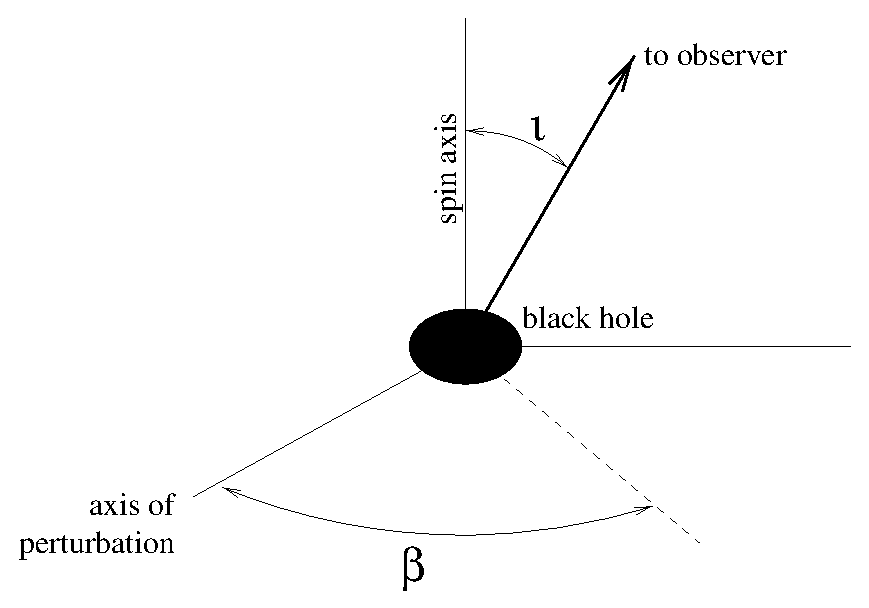
\epsfig{file=Figures/orient.eps,height=6cm}
\caption{\label{f:orient} The polar angle, $\iota$, and the azimuthal angle,
  $\beta$, of the observer relative to the spin axis of a black hole and
  the (somewhat arbitrary) axis of perturbation.}
\end{center}
\end{figure}

The important physical quantities for the study of the gravitational
waves arising from black hole perturbations can be recovered from the
field~$\Psi_4$.  In particular, the ``$+$'' and~``$\times$'' polarizations
of the strain induced by the gravity waves are found
by~\cite{teukolsky:1973}
\begin{equation}
  h_+ - ih_\times = -\frac{2c^2}{|\omega|^2}\,\Psi_4\;.
  \label{e:perturbation strain}
\end{equation}
The quantity~$h_+=h_{\hat\iota\hat\iota}$ is the metric perturbation
that represents the linear polarization state along
${\mathbf{e}}_{\hat\iota}$ and~${\mathbf{e}}_{\hat\beta}$, while the
quantity~$h_\times=h_{\hat\iota\hat\beta}$ represents the linear
polarization state
along~${\mathbf{e}}_{\hat\iota}\pm{\mathbf{e}}_{\hat\beta}$.  The power
radiated towards the observer (per unit solid angle) is
\begin{equation}
  \frac{d^2E}{dt\,d\Omega} = \lim_{r\to\infty}
  \frac{c^7r^2}{4\pi G|\omega|^2} \, |\Psi_4|^2\;.
  \label{e:perturbation power}
\end{equation}
Thus, in order to compute the relevant information about gravitational
waves emitted as perturbations to rotating black hole spacetimes, one
needs to calculate the value of~$\Psi_4$ at large radii from the black hole.

The quasinormal modes are resonant modes of the Teukolsky equation
that describe purely outgoing radiation in the wave-zone and purely
ingoing radiation at the event horizon.  The quasi-normal modes are
described by a spectrum of complex eigenvalues (which include the
spectrum of eigenfrequencies~$\omega_n$), and
eigenfunctions ${}_{-2}R_{\ell m}(r)$
and~${}_{-2}S_{\ell m}(\mu)$ for each value spheroidal mode $\ell$
and~$m$.  These eigenvalues and functions also depend on the mass and
angular momentum of the black hole.  We shall only consider
the fundamental ($n=0$) mode since the harmonics of this mode have
shorter lifetimes.  For the same reason, we are most interested in the
quadrupole ($\ell=2$ and~$m=2$) mode.  The observer is assumed to be at a large
distance; in this case, one can approximate the perturbation as follows:
\begin{equation}
  \Psi_4 \approx \frac{A}{r}\,e^{-i\omega t_{\mathrm{\scriptscriptstyle ret}}}
    {}_{-2}S_{\ell m}(\mu)e^{im\beta}.
  \label{e:asymp perturbation}
\end{equation}
Here $t_{\mathrm{\scriptstyle ret}}=t-r^\star/c$ represents the retarded time,
where~$r^\star$ is a ``tortoise'' radial parameter.  For large radii, the
tortoise radius behaves as $r-r_+\log(r/r_+)$ where~$r_+$ is the ``radius''
of the black hole event horizon.  Thus, we see that the tortoise radius is
nearly equal to the distance of the objects surrounding the black hole,
and we shall view it as the ``distance to the black hole.''  The
parameter~$A$ represents the amplitude of the perturbation, which has the
dimensions of~$[L^{-1}]$.

Given the asymptotic form of the perturbation in
equation~\ref{e:asymp perturbation}, we can integrate
equation~\ref{e:perturbation power} over the entire sphere and the
interval~$t_{\mathrm{\scriptstyle ret}}\in[0,\infty)$ to obtain an expression
for the total energy
radiated in terms of the amplitude~$A$ of the perturbation.  Thus, we can
characterize the amplitude by the total amount of energy emitted:
$A^2=4Gc^{-7}E|\omega|^2(-{\mathrm{Im}}\,\omega)$.  The gravitational waveform
is found to be
\begin{equation}
  h_+ - ih_\times \approx - \frac{4c}{r}
    \biggl(\frac{-{\mathrm{Im}}\,\omega}{|\omega|^2}\biggr)^{1/2}
    \biggl(\frac{GE}{c^5}\biggr)^{1/2}
    e^{-i\omega t_{\mathrm{\scriptscriptstyle ret}}}
    {}_{-2}S_{\ell m}(\mu) e^{im\beta}.
  \label{e:quasinormal ring strain}
\end{equation}
In order to simulate the quasinormal ringing of a black hole, it is necessary
to determine the complex eigenvalues of the desired mode,
and then to compute the spheroidal wave function~$S_{\ell m}(\mu)$.  The
routines to perform these computations are discussed in the following sections.

Rather than computing the actual gravitational strain waveforms at the
detector, the routines will calculate the quantity
$H_+-iH_\times=(c^2r/GM_\odot)(h_+-ih_\times)$; the normalization
of these waveforms to the correct source distance is left to the calling
routine.  The distance normalization can be computed as follows:
\begin{equation}
  \frac{c^2r}{GM_\odot} = \frac{r}{T_\odot c}
    = \biggl( \frac{r}{1.4766\,{\mathrm{km}}} \biggr)
    = 2.090\times10^{19}\biggl( \frac{r}{\mathrm{Mpc}} \biggr).
  \label{e:radius in solar masses}
\end{equation}
where $T_\odot=4.925491\,\mu{\mathrm{s}}$ is the mass of the sun expressed in
seconds (see equation~\ref{e:tsolar}).
It will be convenient to write the time dependence of the strain as the
complex function~${\mathcal{H}}(t_{\mathrm{\scriptstyle ret}})$ so that
$H_+-iH_\times={\mathcal{H}}(t_{\mathrm{\scriptstyle ret}})
 {}_{-2}S_{\ell m}(\mu)e^{im\beta}$.
The dimensionless eigenfrequency, $\hat{\omega}=GM\omega/c^3$,
depends only on the mode and the dimensionless
angular momentum of the black hole.  In terms of this quantity,
the function~${\mathcal{H}}(t_{\mathrm{\scriptstyle ret}})$ is
\begin{equation}
  {\mathcal{H}}(t_{\mathrm{\scriptstyle ret}}) \approx -4 \epsilon^{1/2}
    \frac{(-{\mathrm{Im}}\,\hat{\omega})^{1/2}}{|\hat{\omega}|}
    \biggl(\frac{M}{M_\odot}\biggr)
    \exp\biggl[-i\hat{\omega}\biggl(
      \frac{t_{\mathrm{\scriptstyle ret}}}{T_\odot}\biggr)
      \biggl(\frac{M}{M_\odot}\biggr)^{-1}\biggr]
  \label{e:dimensionless strain function}
\end{equation}
where $\epsilon$ is the fractional mass loss due to the radiation in the
excited quasinormal mode.


\clearpage
\subsection{Function: \texttt{qn\_eigenvalues()}}
\label{ss:qn_eigenvalues}

\begin{verbatim}
void qn_eigenvalues(float eigenvalues[], float a, int s, int l, int m)
\end{verbatim}
This routine computes the eigenvalues associated with the spheroidal and
radial wave functions for a specified quasinormal mode.  The arguments are:
\begin{description}
\item{\texttt{eigenvalues}}: Output.  An array, \texttt{eigenvalues[0..3]},
  which contains, on output, the real and imaginary parts of the eigenvalues
  $\hat{\omega}$ and~$A$ (see below) as follows:
  $\texttt{eigenvalues[0]}={\mathrm{Re}}\,\hat{\omega}$,
  $\texttt{eigenvalues[1]}={\mathrm{Im}}\,\hat{\omega}$,
  $\texttt{eigenvalues[2]}={\mathrm{Re}}\,A$,
  and~$\texttt{eigenvalues[3]}={\mathrm{Im}}\,A$.
\item{\texttt{a}}: Input.  The dimensionless angular momentum parameter
  of the Kerr black hole, $|\hat{a}|\le1$, which is negative if the black hole
  is spinning clockwise about the~$\iota=0$ axis (see figure~\ref{f:orient}).
\item{\texttt{s}}: Input.  The integer-valued spin-weight~$s$, which should
  be set to $0$~for a scalar perturbation (e.g., a scalar field perturbation),
  $\pm1$~for a vector perturbation (e.g., an electromagnetic field
  perturbation), or $\pm2$ for a spin two perturbation (e.g., a gravitational
  perturbation).
\item{\texttt{l}}: Input.  The mode integer~$\texttt{l}\ge|\texttt{s}|$.
\item{\texttt{m}}: Input.  The mode integer~$|\texttt{m}|\le\texttt{l}$.
\end{description}

For a Kerr black hole of a given dimensionless angular momentum parameter,
$\hat{a}$, with a
perturbation of spin-weight~$s$ and mode $\ell$ and~$m$, there is a spectrum
of quasinormal modes which are specified by the eigenvalues $\hat{\omega}_n$
and~$A_n$.  As discussed in the previous subsection, the
eigenvalue~$\hat{\omega}_n$ is associated with the separation of the time
dependence of the perturbation, and it specifies the frequency and damping
time of the radiation from the perturbation.  The additional complex
eigenvalue~$A_n$ results from the separation of the radial and azimuthal
dependence into the spheroidal and radial wave functions.  Both of these
eigenvalues will be necessary for the computation of the spheroidal wave
function (below).

The routine \texttt{qn\_eigenvalues()} can be used to compute the eigenvalues
of the fundamental ($n=0$) mode.  To convert the dimensionless eigenvalue
$\hat{\omega}$ to the (complex) frequency of the ringdown of a Kerr black
hole of mass~$M$, one simply computes~$\omega=c^3\hat{\omega}/GM$.
The eigenfrequency is computed using the method of Leaver~\cite{leaver:1985}.
Note that Leaver adopts units in which~$2M=1$, so one finds that
$\hat{\omega}=\frac{1}{2}\omega_{\mathrm{\scriptscriptstyle Leaver}}$ and
$\hat{a}=2a_{\mathrm{\scriptscriptstyle Leaver}}$ in our notation.
The eigenvalues satisfy the following symmetry: if $\rho_m=-i\hat{\omega}_m$
and~$A_m$ are the eigenvalues for an azimuthal index~$m$, then
$\rho_{-m}=\rho_m^\ast$ and~$A_{-m}=A_m^\ast$ are the eigenvalues for the
azimuthal index~$-m$.

\begin{description}
\item{Author:} Jolien Creighton, jolien@tapir.caltech.edu
\item{Comment:} For simplicity, we require that the spin-weight
number, $s$, be an integer.  Thus, the spinor perturbations $\chi_0$
and~$\chi_1$, associated with $s=\pm\frac{1}{2}$
respectively~\cite{teukolsky:1973}, are not allowed.
\end{description}


\clearpage
\subsection{Example: \texttt{eigenvalues} program}

This example uses the function \texttt{qn\_eigenvalues()} to compute the
eigenvalues ${}_s\hat{\omega}_{\ell m}$ and~${}_sA_{\ell m}$ for the
$s$~spin-weighted quasinormal mode specified by $\ell$ and~$m$, and for
a range of values of the dimensionless angular momentum parameter, $\hat{a}$.
To invoke the program, type:
\begin{quote}
\texttt{eigenvalues} $s$ $\ell$ $m$
\end{quote}
for the desired (integer) values of $s$, $\ell$, and~$m$.  Make sure that
$\ell\ge|s|$ and~$0\le m\le\ell$ (the eigenvalues for negative values of
$m$ can be inferred from the symmetries discussed in
subsection~\ref{ss:qn_eigenvalues}).  The output of the program is five
columns of data: the first column is the value of~$\hat{a}$ running from just
greater than~$-1$ to just less than~$1$ (or between $0$ and~$1$ if $m=0$),
the second and third columns are the real and imaginary parts of the
eigenfrequency~$\hat{\omega}$, and the fourth and fifth columns are the
real and imaginary parts of the angular separation eigenvalue~$A$.
For the values of~$\hat{a}<0$, the eigenvalues correspond to the mode
with azimuthal index~$-m$ so that the real part of the eigenfrequency is
positive.  A plot of the eigenfrequency output of the program
\texttt{eigenvalues} for several runs with~$s=-2$ is shown in
figure~\ref{f:eigen}.  The blue curves in figure~\ref{f:eigen} can be compared
to figure~5 of reference~\cite{onozawa:1997} keeping in mind the conversion
factors between Leaver's convention (which is also used in~\cite{onozawa:1997})
and the convention used here (see subsection~\ref{ss:qn_eigenvalues}).

\begin{figure}[h]
\index{colorpage}
\begin{center}
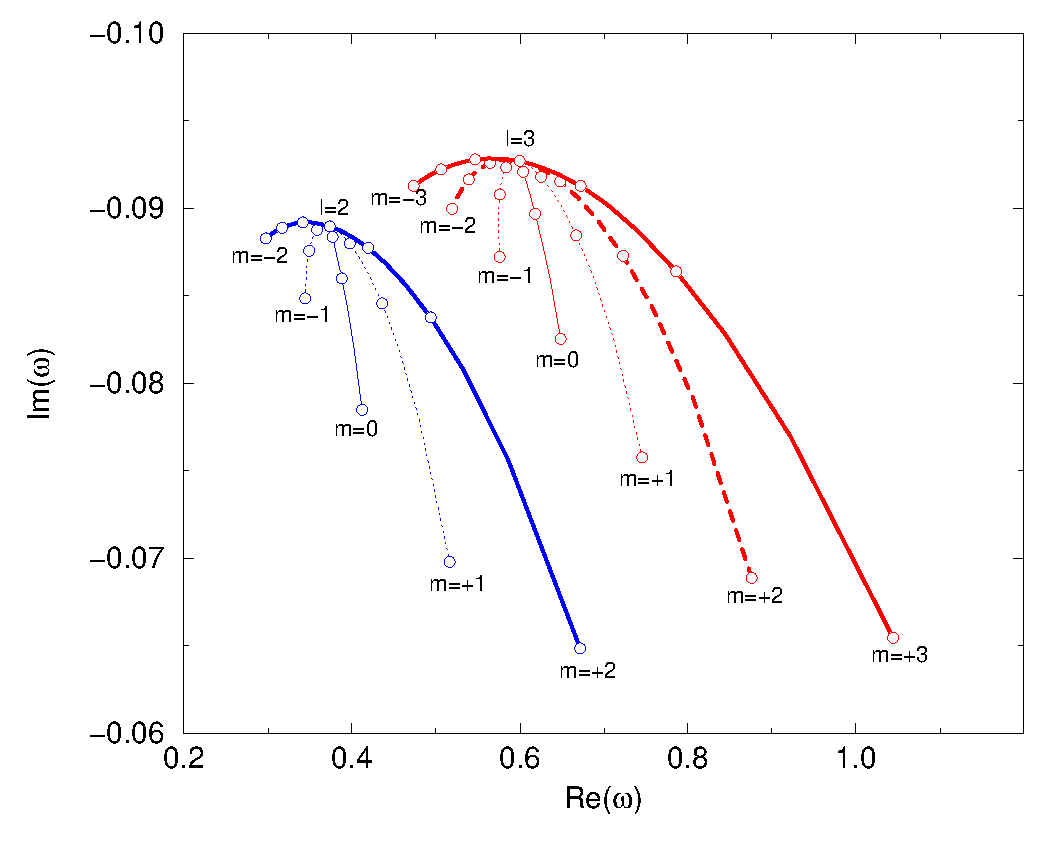
\epsfig{file=Figures/eigen.eps,height=7.5cm}
\caption{\label{f:eigen} The real and imaginary parts of the eigenfrequencies,
  $\hat{\omega}$, as computed by the program \texttt{eigenvalues} with $s=-2$.
  Each curve corresponds to a range of values of $\hat{a}$ from $-0.9$ (left)
  to~$+0.9$ (right) for a single mode $\ell$ and $|m|$.  The open circles are
  placed at the values $\hat{a}=-0.9$, $-0.6$, $-0.3$, $0$, $+0.3$, $+0.6$,
  and~$+0.9$ except when $m=0$ in which case there are no negative values
  of~$\hat{a}$ plotted.  The blue curves correspond to the $\ell=2$ modes and
  the red curves correspond to the $\ell=3$ modes.}
\end{center}
\end{figure}

\clearpage
\lgrindfile{Includes/eigenvalues.tex}

\begin{description}
\item{Author:} Jolien Creighton, jolien@tapir.caltech.edu
\end{description}


\clearpage
\subsection{Function: \texttt{sw\_spheroid()}}
\label{ss:sw_spheroid}

\begin{verbatim}
void sw_spheroid(float *re, float *im, float mu, int reset,
                 float a, int s, int l, int m, float eigenvalues[])
\end{verbatim}
This routine computes the spin-weighted spheroidal wave
function~${}_sS_{\ell m}(\mu)$.  The arguments are:
\begin{description}
\item{\texttt{re}}: Output.  The real part of the spin-weighted spheroidal
  wave function.
\item{\texttt{im}}: Output.  The imaginary part of the spin-weighted spheroidal
  wave function.
\item{\texttt{mu}}: Input.  The independent variable, $\mu=\cos\iota$ with
  $\iota$ being a polar angle, of the spin-weighted spheroidal wave function;
  $-1<\texttt{mu}<1$.
\item{\texttt{reset}}: Input.  A flag that indicates that the function should
  reset ($\texttt{reset}=1$) the internally stored normalization of the
  spin-weighted spheroidal wave function.  The reset flag should be set
  if any of the following five arguments are changed between calls; otherwise,
  set $\texttt{reset}=0$ so that the routine does not recompute the
  normalization.
\item{\texttt{a}}: Input.  The dimensionless angular momentum parameter,
  $-1<\texttt{a}<1$, of the Kerr black hole for which the spin-weighted
  spheroidal wave function is associated.
\item{\texttt{s}}: Input.  The integer-valued spin-weight~$s$, which should
  be set to $0$~for a scalar perturbation (e.g., a scalar field perturbation),
  $\pm1$~for a vector perturbation (e.g., an electromagnetic field
  perturbation), or $\pm2$ for a spin two perturbation (e.g., a gravitational
  perturbation).
\item{\texttt{l}}: Input.  The mode integer~$\texttt{l}\ge|\texttt{s}|$.
\item{\texttt{m}}: Input.  The mode integer~$|\texttt{m}|\le\texttt{l}$.
\item{\texttt{eigenvalues}}: Input.  An array, \texttt{eigenvalues[0..3]},
  which contains the real and imaginary parts of the eigenvalues
  $\hat{\omega}$ and~$A$ (see below) as follows:
  $\texttt{eigenvalues[0]}={\mathrm{Re}}\,\hat{\omega}$,
  $\texttt{eigenvalues[1]}={\mathrm{Im}}\,\hat{\omega}$,
  $\texttt{eigenvalues[2]}={\mathrm{Re}}\,A$,
  and~$\texttt{eigenvalues[3]}={\mathrm{Im}}\,A$.  These may be calculated for
  a quasinormal mode using the routine \texttt{qn\_eigenvalues()}.
\end{description}

The spin-weighted spheroidal wave function
is also computed using the method of Leaver~\cite{leaver:1985}.
We have adopted the following normalization criteria for the spin-weighted
spheroidal wave functions~${}_sS_{\ell m}(\mu)$.  First, the angle-averaged
value of the squared modulus of~${}_sS_{\ell m}(\mu)$ is unity:
$\int_{-1}^{1}|{}_sS_{\ell m}(\mu)|^2d\mu=1$.  Second, the complex phase is
partially fixed by the requirement that ${}_sS_{\ell m}(0)$ is real.
Finally, the sign is set to be $(-)^{\ell-\max(m,s)}$ for the real part
in the limit that
$\mu\to-1$ in order to agree with the sign of the spin-weighted spherical
harmonics~${}_sY_{\ell m}(\mu,0)$ (see~\cite{goldberg:1967}).

It is sufficient to compute the spin-weighted spheroidal wave functions
with $s<0$ and~$a\omega=\hat{a}\hat{\omega}\ge0$ because of the following
symmetries~\cite{press:1973}:
\begin{equation}
  {}_{-s}S_{\ell m}(\mu,a\omega) = {}_sS_{\ell m}(-\mu,a\omega)
  \quad {\textrm{with}} \quad
  {}_{-s}E_{\ell m}(a\omega) = {}_sE_{\ell m}(a\omega)
\end{equation}
and
\begin{equation}
  {}_sS_{\ell m}(\mu,-a\omega) = {}_sS_{\ell,-m}(-\mu,a\omega)
  \quad {\textrm{with}} \quad
  {}_sE_{\ell m}(-a\omega) = {}_sE_{\ell,-m}(a\omega)
\end{equation}
where ${}_sE_{\ell m}={}_sA_{\ell m}+s(s+1)$.

\begin{description}
\item{Author:} Jolien Creighton, jolien@tapir.caltech.edu
\end{description}


\clearpage
\subsection{Example: \texttt{spherical} program}

The program \texttt{spherical} is an example implementation of the
routine \texttt{sw\_spheroid()} to compute the standard spin-weighted
spherical harmonics~\cite{goldberg:1967}.  The program also computes these
functions using equation~(3.1) of~\cite{goldberg:1967} for comparison.
According to the normalization convention stated in
subsection~\ref{ss:sw_spheroid}, the relationship between the spin-weighted
spheroidal harmonics and the spin-weighted spherical harmonics is:
\begin{equation}
  {}_sY_{\ell m}(\theta,\phi) =
    (2\pi)^{-1/2}{}_sS_{\ell m}(\cos\theta)e^{im\phi}
\end{equation}
with $a\omega=0$ and~$A=(\ell-s)(\ell+s+1)$.

To invoke the program, type:
\begin{quote}
  \texttt{spherical} $s$ $\ell$ $m$
\end{quote}
for the desired (integer) values of $s$, $\ell$, and~$m$
($\ell\ge|s|$ and~$|m|\le\ell$).  The output is three columns of data: the
first column is the independent variable~$\mu$ between $-1$ and~$+1$, the
second column is the value of~$(2\pi)^{-1/2}{}_sS_{\ell m}(\mu)$, and the
third column is the value of~${}_sY_{\ell m}(\mu,0)$ as computed from
equation~(3.1) of~\cite{goldberg:1967}.  A comparison of the results produced
by the program \texttt{spherical} for $\ell=m=-s=2$ with the exact values
of ${}_{-2}Y_{22}(\mu,0)=(5/64\pi)^{1/2}(1+\mu)^2$ is shown in
table~\ref{t:spherical harmonic}.

\begin{table}[h]
\begin{center}
\begin{tabular}{|cccc|}
  \hline
  $\mu$ & Goldberg & \texttt{sw\_spheroid()} & exact \\
  \hline\hline
  $-0.99$ & $1.576955\times10^{-5}$ & $1.576955\times10^{-5}$ 
          & $1.576958\times10^{-5}$ \\
  $-0.95$ & $3.942387\times10^{-4}$ & $3.942387\times10^{-4}$
          & $3.942395\times10^{-4}$ \\
  $-0.75$ & $9.855968\times10^{-3}$ & $9.855967\times10^{-3}$
          & $9.855986\times10^{-3}$ \\
  $-0.55$ & $3.193334\times10^{-2}$ & $3.193333\times10^{-2}$
          & $3.193340\times10^{-2}$ \\
  $-0.35$ & $6.662639\times10^{-2}$ & $6.662639\times10^{-2}$
          & $6.663647\times10^{-2}$ \\
  $-0.15$ & $1.139351\times10^{-1}$ & $1.139351\times10^{-1}$
          & $1.139352\times10^{-1}$ \\
  $+0.15$ & $2.085525\times10^{-1}$ & $2.085525\times10^{-1}$
          & $2.085527\times10^{-1}$ \\
  $+0.35$ & $2.874004\times10^{-1}$ & $2.874005\times10^{-1}$
          & $2.874006\times10^{-1}$ \\
  $+0.55$ & $3.788640\times10^{-1}$ & $3.788639\times10^{-1}$
          & $3.788641\times10^{-1}$ \\
  $+0.75$ & $4.829430\times10^{-1}$ & $4.829430\times10^{-1}$
          & $4.829433\times10^{-1}$ \\
  $+0.95$ & $5.996378\times10^{-1}$ & $5.996379\times10^{-1}$
          & $5.996382\times10^{-1}$ \\
  $+0.99$ & $6.244906\times10^{-1}$ & $6.244906\times10^{-1}$
          & $6.244911\times10^{-1}$ \\
  \hline
\end{tabular}
\end{center}
\caption{\label{t:spherical harmonic}
  A comparison of the values of the spin-weighted spherical harmonic
  ${}_{-2}Y_{22}(\mu,0)$ calculated by equation~(3.1) of
  Goldberg~\protect\cite{goldberg:1967}, the values of
  $(2\pi)^{-1/2}{}_{-2}S_{22}(\mu)$ using routine \texttt{sw\_spheroid()},
  and the values of the exact result $(5/64\pi)^{1/2}(1+\mu)^2$.  The three
  methods give excellent agreement.}
\end{table}

\clearpage
\lgrindfile{Includes/spherical.tex}

\begin{description}
\item{Author:} Jolien Creighton, jolien@tapir.caltech.edu
\end{description}


\clearpage
\subsection{Example: \texttt{spheroid} program}

This is a second implementation of the function \texttt{sw\_spheroid()}
which is used to compute the spin-weighted spheroidal wave function
associated with a quasinormal ringdown mode of a Kerr black hole with
a certain (specified in the code) dimensionless angular momentum parameter.  
To invoke the program, type:
\begin{quote}
  \texttt{spheroid} $s$ $\ell$ $m$
\end{quote}
for the desired (integer) values of $s$, $\ell$, and~$m$
($\ell\ge|s|$ and~$|m|\le\ell$) of the desired mode.
The output is three columns of data: the
first column is the independent variable~$\mu$ between $-1$ and~$+1$, the
second column is the value of the real part of~${}_sS_{\ell m}(\mu)$, and the
third column is the value of the imaginary part of~${}_sS_{\ell m}(\mu)$.
Figure~\ref{f:spheroid} depicts the output for the spin-weighted spheroidal
wave function~${}_{-2}S_{22}(\mu)$.

\begin{figure}[h]
\begin{center}
\index{colorpage}
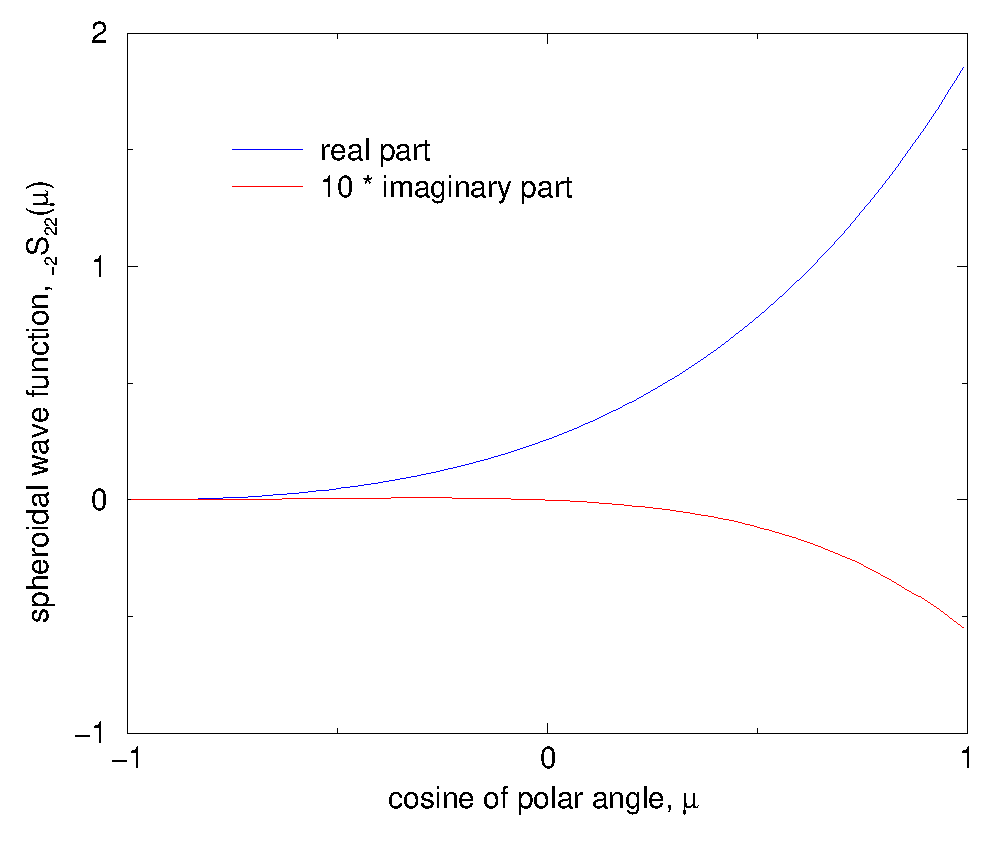
\epsfig{file=Figures/spheroid.eps,height=7.5cm}
\caption{\label{f:spheroid} A plot of the real and imaginary parts of the
  $\ell=m=-s=2$ spin-weighted spheroidal wave function, ${}_{-2}S_{22}(\mu)$,
  associated with a black hole with dimensionless angular momentum
  parameter~$\hat{a}=0.98$.  The imaginary part is scaled by a factor of ten.}
\end{center}
\end{figure}

\clearpage
\lgrindfile{Includes/spheroid.tex}

\begin{description}
\item{Author:} Jolien Creighton, jolien@tapir.caltech.edu
\end{description}


\clearpage
\subsection{Function: \texttt{qn\_ring()}}

\begin{verbatim}
int qn_ring(float iota, float beta,
            float eps, float M, float a, int l, int m,
            float dt, float atten, int max,
            float **plusPtr, float **crossPtr)
\end{verbatim}
This routine is used to compute the ``$+$'' and~``$\times$'' polarizations
of the gravitational waveform, $H(t_{\mathrm{\scriptstyle ret}})$, produced by
a black hole ringdown at a distance
$GM_\odot/c^2=T_\odot c\simeq1.4766\,{\mathrm{km}}$.  To obtain the waveforms
at a distance~$r$, multiply the result by $GM_\odot/c^2r=T_\odot c/r$.
The arguments are:
\begin{description}
\item{\texttt{iota}}: Input.  The polar angle (inclination), $\iota$
  (in radians), of
  the sky position of the observer with respect to the (positive) spin axis
  of the black hole, $0\le\texttt{iota}\le\pi$.
\item{\texttt{beta}}: Input.  The azimuth, $\beta$ (in radians),
  of the sky position
  of the observer with respect to the axis of the perturbation at the start
  time.  ($0\le\texttt{beta}\le2\pi$.)
\item{\texttt{eps}}: Input.  The fraction of the total mass lost
  in gravitational radiation from the particular mode. ($0<\texttt{eps}\ll1$.)
\item{\texttt{M}}: Input.  The mass of the black hole in solar masses.
\item{\texttt{a}}: Input.  The dimensionless angular momentum parameter
  of the Kerr black hole, $|\hat{a}|\le1$, which is negative if the black hole
  is spinning clockwise about the~$\iota=0$ axis (see figure~\ref{f:orient}).
\item{\texttt{l}}: Input.  The mode integer $\ell$.  ($\texttt{l}\ge2$)
\item{\texttt{m}}: Input.  The mode integer $m$.  ($|\texttt{m}|\le\texttt{l}$)
\item{\texttt{dt}}: Input.  The time interval, in seconds, between successive
  data points in the returned waveforms.
\item{\texttt{atten}}: Input.  The attenuation level, in dB, at which the
  routine will terminate calculation of the waveforms.  I.e., the routine
  will terminate when the amplitude,
  $A=A_0\exp(-{\mathrm{Im}}\,\omega t_{\mathrm{\scriptstyle ret}})$, falls below
  the level~$A_{\mathrm{\scriptstyle cutoff}}=A_0\,{\mathrm{alog}}_{10}(-0.1\times
  \texttt{atten})$.
\item{\texttt{max}}: Input.  The maximum number of data points to be returned
  in the waveforms.
\item{\texttt{plusPtr}}: Input/Output.  A pointer to an array which, on
  return, contains the waveform~$H_+$ sampled at intervals \texttt{dt}.
  If the array has the value \texttt{NULL} on input, the routine allocates
  an amount of memory to \texttt{*plusPtr} to hold \texttt{max} elements.
\item{\texttt{crossPtr}}: Input/Output.  A pointer to an array which, on
  return, contains the waveform~$H_\times$ sampled at intervals \texttt{dt}.
  If the array has the value \texttt{NULL} on input, the routine allocates
  an amount of memory to \texttt{*crossPtr} to hold \texttt{max} elements.
\end{description}

The routine \texttt{qn\_ring()} returns the number of data points that were
written to the arrays \texttt{(*plusPtr)[]} and \texttt{(*crossPtr)[]}; this
is either the number specified by the input parameter \texttt{max} or the
number of points computed when the waveform was attenuated by the threshold
\texttt{atten}.  The eigenvalues are obtained from the function
\texttt{qn\_eigenvalues()}.  The waveform is
then computed using $H_+-iH_\times={\mathcal{H}}(t_{\mathrm{\scriptstyle ret}})
 {}_{-2}S_{\ell m}(\mu)e^{im\beta}$
with~${\mathcal{H}}(t_{\mathrm{\scriptstyle ret}})$ given by
equation~(\ref{e:dimensionless strain function}).  The spheroidal wave function
is obtained from the function \texttt{sw\_spheroid()}.

\begin{description}
\item{Author:} Jolien Creighton, jolien@tapir.caltech.edu
\end{description}


\clearpage
\subsection{Example: \texttt{ringdown} program}

This example uses the function \texttt{qn\_ring()} to compute the black hole
quasinormal ringdown waveform for a preset mode and inclination.  The waveform
as a function of time is written to standard output in three columns: the time,
the plus polarization, and the cross polarization.  A Plot of the quasinormal
ringdown waveform data is shown in figure~\ref{f:ring}.

\begin{figure}[h]
\begin{center}
\index{colorpage}
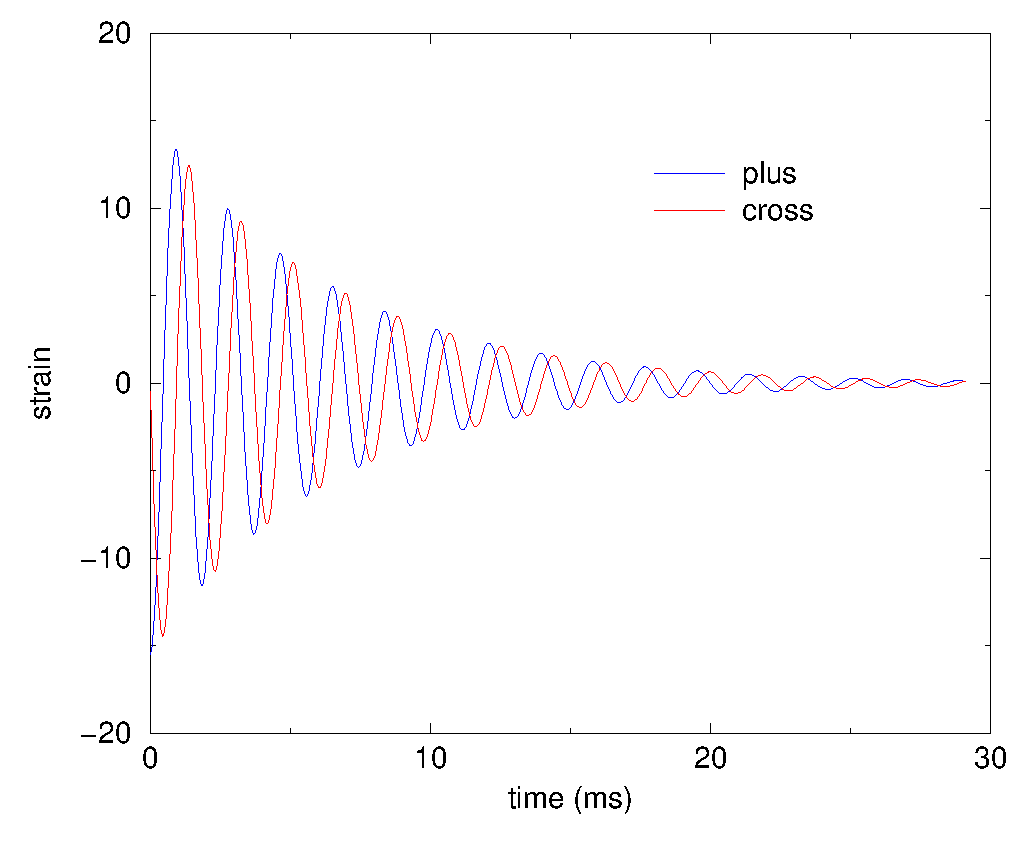
\epsfig{file=Figures/ring.eps,height=7.5cm}
\caption{\label{f:ring} A plot of the plus and cross polarizations of the
  gravitational wave strain, at a (unphysical!)
  distance~$GM_\odot/c^2=T_\odot c\simeq1.4766\,{\mathrm{km}}$,
  for the fundamental
  $\ell=m=2$ mode of a black hole with mass $M=50M_\odot$, dimensionless
  angular momentum parameter~$0.98$, and fractional mass loss $\epsilon=0.03$,
  with inclination and azimuth $\iota=0$ and~$\beta=0$.  The data was produced
  by the program \texttt{ringdown}.}
\end{center}
\end{figure}

\clearpage
\lgrindfile{Includes/ringdown.tex}

\begin{description}
\item{Author:} Jolien Creighton, jolien@tapir.caltech.edu
\end{description}


\clearpage
\subsection{Function: \texttt{qn\_qring()}}

\begin{verbatim}
int qn_qring(float psi0, float eps, float M, float a,
             float dt, float atten, int max, float **strainPtr)
\end{verbatim}
The routine \texttt{qn\_qring()} is a quick ringdown generator which constructs
a damped sinusoid with a frequency and quality approximately equal to that
of the $\ell=m=2$ quasinormal mode of a Kerr black hole and an amplitude
approximately equal to angle-averaged strain expected for black hole radiation
at a distance $GM_\odot/c^2=T_\odot c\simeq1.4766\,{\mathrm{km}}$.  To obtain
the waveforms at a distance~$r$, multiply the result
by~$GM_\odot/c^2r=T_\odot c/r$.  The arguments to the routine are:
\begin{description}
\item{\texttt{psi0}}: Input.  The initial phase (in radians) of the waveform
  (see below).
\item{\texttt{eps}}: Input.  The fractional mass loss in quadrupolar
  ($\ell=m=2$) radiation.  ($0<\texttt{eps}\ll1$.)
\item{\texttt{M}}: Input.  The mass of the black hole in solar masses.
\item{\texttt{a}}: Input.  The dimensionless angular momentum parameter
  of the Kerr black hole, $|\hat{a}|\le1$, which is negative if the black hole
  is spinning clockwise about the~$\iota=0$ axis (see figure~\ref{f:orient}).
\item{\texttt{dt}}: Input. The time interval, in seconds, between successive
  data points in the returned waveform.
\item{\texttt{atten}}: Input:  The attenuation level, in dB, at which the
  routine will terminate calculation of the waveforms.
\item{\texttt{max}}: Input.  The maximum number of data points to be returned
  in the waveforms.
\item{\texttt{strainPtr}}: Input/Output.  A pointer to an array which, on
  return, contains the angle-averaged waveform sampled at intervals
  \texttt{dt}.  If the array has the value \texttt{NULL} on input, the routine
  allocates an amount of memory to \texttt{*strainPtr} to hold \texttt{max}
  elements.
\end{description}

The routine \texttt{qn\_ring()} returns the number of data points that were
written to the array \texttt{(*strainPtr)[]}; this
is either the number specified by the input parameter \texttt{max} or the
number of points computed when the waveform was attenuated by the threshold
\texttt{atten}.  The array contains the \emph{angle averaged waveform}
\begin{equation}
    H_{\mathrm{\scriptstyle ave}}(t_{\mathrm{\scriptstyle ret}}) =
    \frac{1}{\surd5} {\mathrm{Re}}\,\bigl[
    {\mathcal{H}}(t_{\mathrm{\scriptstyle ret}}) e^{i\psi_0} \bigr],
\end{equation}
where ${\mathcal{H}}(t_{\mathrm{\scriptstyle ret}})$ is given by
equation~(\ref{e:dimensionless strain function}), sampled at time
intervals~$dt$.  The constant~$\psi_0$ defines the initial phase of the
waveform.  The amplitude factor is set by the following argument:
The gravitational strain (at a distance
$GM_\odot/c^2=T_\odot c\simeq1.4766\,{\mathrm{km}}$)
that would be observed by an interferometer is
given by~$H(t_{\mathrm{\scriptstyle ret}})=F_+(\theta,\phi,\psi)
 H_+(t_{\mathrm{\scriptstyle ret}},\iota,\beta)
 + F_\times(\theta,\phi,\psi)
 H_\times(t_{\mathrm{\scriptstyle ret}},\iota,\beta)$ where $F_+$
and~$F_\times$ represent the antenna patterns of the interferometer.
When averaged over $\theta$, $\phi$, and~$\psi$, one finds
$\langle F_+^2\rangle=\langle F_\times^2\rangle=\frac{1}{5}$
and~$\langle F_+F_\times\rangle=0$.  Thus,
\begin{eqnarray}
  \langle H^2(t_{\mathrm{\scriptstyle ret}})
    \rangle_{\theta,\phi,\psi,\iota,\beta}
  &=& {\textstyle\frac{1}{5}} \langle
      H_+^2(t_{\mathrm{\scriptstyle ret}},\iota,\beta)
      + H_\times^2(t_{\mathrm{\scriptstyle ret}},\iota,\beta)
      \rangle_{\iota,\beta} \nonumber\\
  &=& {\textstyle\frac{1}{5}} \langle
      | (H_+ - iH_\times)(t_{\mathrm{\scriptstyle ret}},\iota,\beta) |^2
      \rangle_{\iota,\beta} \nonumber\\
  &=& {\textstyle\frac{1}{10}} |{\mathcal{H}}(t_{\mathrm{\scriptstyle ret}})|^2
      \nonumber\\
  &\approx& \overline{H_{\mathrm{\scriptstyle ave}}^2}
\end{eqnarray}
where the overbar indicates a time average over a single cycle; approximate
equality becomes exact in the limit of a high quality ringdown.  It is in
this sense that the
quantity~$H_{\mathrm{\scriptstyle ave}}(t_{\mathrm{\scriptstyle ret}})$ can be
viewed as an angle-averaged waveform.

Rather than compute the eigenfrequency using the routine
\texttt{qn\_eigenvalues()}, this routine uses the analytic fits to the
eigenfrequency found by Echeverria~\cite{echeverria:1989}.
These expressions are:
\begin{equation}
  \hat{\omega} \simeq f(\hat{a}) \bigl( 1 - {\textstyle\frac{1}{4}}ig(\hat{a})
  \bigr)
\end{equation}
with
\begin{eqnarray}
  f(\hat{a}) &=& 1 - 0.63(1-\hat{a})^{3/10} \\
  g(\hat{a}) &=& (1-\hat{a})^{9/20}.
\end{eqnarray}

\begin{description}
\item{Author:}  Jolien Creighton, jolien@tapir.caltech.edu
\item{Comments:}  Since this routine does not need to compute the spheroidal
  wave function and uses an analytic approximation to the eigenfrequency,
  it is much simpler than the routine \texttt{qn\_ring()}.  The approximate
  eigenfrequencies are typically accurate to within~$\sim5\%$, so this routine
  is to be preferred when computing quadrupolar $(\ell=m=2)$ quasinormal
  waveforms unless accuracy is critical.
\end{description}


\clearpage
\subsection{Function: \texttt{qn\_filter()}}

\begin{verbatim}
int qn_filter(float freq, float qual,
              float dt, float atten, int max, float **filterPtr)
\end{verbatim}
Quasinormal ringdown waveforms are characterized by two parameters:
the central frequency of the waveform, and the \emph{quality} of the
waveform.  The parameter space is most easily described in terms of
these variables (rather than the mass and the angular momentum of the
corresponding black hole), so it is useful to construct filters for
quasinormal ringdown waveform searches in terms of the frequency and
quality of the waveform.  This routine constructs such a filter, with
a specified frequency and quality.  The routine returns
the number of filter elements computed before a specified attenuation
level was reached.  The arguments are:
\begin{description}
\item{\texttt{freq}}: Input.  The central frequency, in Hertz, of the
  ringdown filter.
\item{\texttt{qual}}: Input.  The quality of the ringdown filter.
\item{\texttt{dt}}: Input. The time interval, in seconds, between successive
  data points in the returned waveform.
\item{\texttt{atten}}: Input:  The attenuation level, in dB, at which the
  routine will terminate calculation of the waveforms.
\item{\texttt{max}}: Input.  The maximum number of data points to be returned
  in the waveforms.
\item{\texttt{filterPtr}}: Input/Output.  A pointer to an array which, on
  return, contains the filter sampled at intervals
  \texttt{dt}.  If the array has the value \texttt{NULL} on input, the routine
  allocates an amount of memory to \texttt{*filterPtr} to hold \texttt{max}
  elements.
\end{description}

The constructed filter, $q(t)$, is the function
\begin{equation}
  q(t) = e^{-\pi ft/Q}\cos(2\pi ft)
\end{equation}
where $f$ is the central frequency and~$Q$ is the quality.  The routine
\texttt{qn\_filter()} performs no normalization, nor does it account for
different possible starting phases.  The latter is not important for
detection template construction.  Normalization is achieved using the
function \texttt{qn\_normalize()}, which is described later.

\begin{description}
\item{Author:}  Jolien Creighton, jolien@tapir.caltech.edu
\end{description}


\clearpage
\subsection{Function: \texttt{qn\_normalize()}}

\begin{verbatim}
void qn_normalize(float *u, float *q, float *r, int n, float *norm)
\end{verbatim}
Given a filter, $\tilde{q}(f)$, and twice the inverse power spectrum, $r(f)$,
this routine generates a normalized template~$\tilde{u}(f)$ for which
$1=\langle N^2\rangle\to\frac{1}{2}\texttt{correlate(\ldots,u,u,r,n)}$.
The arguments are:
\begin{description}
\item{\texttt{u}}: Output.  The array \texttt{u[0..n-1]} contains the
  positive frequency part of the complex template function~$\tilde{u}(f)$,
  packed as described in the Numerical Recipes routine \texttt{realft()}.
\item{\texttt{q}}: Input.  The array \texttt{q[0..n-1]} contains the
  positive frequency part of the complex filter function~$\tilde{q}(f)$, also
  packed as described in the Numerical Recipes routine \texttt{realft()}.
\item{\texttt{r}}: Input.  The array \texttt{r[0..n/2]} contains the values
  of the real function $r(f)=2/S_h(|f|)$ used as a weight in the
  normalization.  The array elements are arranged in order of increasing
  frequency from the DC component at subscript~0 to the Nyquist frequency
  at subscript~\texttt{n}/2.
\item{\texttt{n}}: Input.  The total length of the arrays \texttt{u} and
  \texttt{q}.  Must be even.
\item{\texttt{norm}}: Output.  The normalization constant, $\alpha$, defined
  below.
\end{description}

Given a filter, $q(t)$, this routine computes a template, $u(t)=\alpha q(t)$,
which is normalized so that $(u,u)=2$, where~$(\cdot,\cdot)$ is the inner
product defined by equation~(\ref{e:definprod}).  Thus, the normalization
constant is given by
\begin{equation}
  \frac{1}{\alpha^2} = \frac{1}{2}(q,q).
\end{equation}

\begin{description}
\item{Author:}  Jolien Creighton, jolien@tapir.caltech.edu
\end{description}


\clearpage
\subsection{Function: \texttt{find\_ring()}}

\begin{verbatim}
void find_ring(float *h, float *u, float *r, float *o,
               int n, int len, int safe, int *off,
               float *snr, float *mean, float *var)
\end{verbatim}
This optimally filters the strain data using an input template
and then finds the time at which the SNR peaks.  The arguments are:
\begin{description}
\item{\texttt{h}}: Input.  The FFT of the strain data~$\tilde{h}(f)$.
\item{\texttt{u}}: Input.  The normalized template~$\tilde{u}(f)$.
\item{\texttt{r}}: Input.  Twice the inverse power spectrum~$2/S_h(|f|)$.
\item{\texttt{o}}: Output.  Upon return, contains the filter output.
\item{\texttt{n}}: Input.  Defines the lengths of the arrays
  \texttt{h[0..n-1]}, \texttt{u[0..n-1]}, \texttt{o[0..n-1]},
  and \texttt{r[0..n/2]}.
\item{\texttt{len}}: Input.  The number of time domain bins for which
  the filter~$u(t)$ is non-zero.  Needed in order to eliminate the wrap-around
  ambiguity described in subsection~\ref{ss:dirty}.
\item{\texttt{safe}}: Input.  The additional number of time domain bins to use
  as a safety margin.  This number of points are ignored at the beginning of
  the filter output and, along with the number of points \texttt{len}, at the
  ending of the filter output.  Needed in order to eliminate the wrap-around
  ambiguity described in subsection~\ref{ss:dirty}.
\item{\texttt{off}}: Output.  The offset, in the range \texttt{safe} to
  \texttt{n-len-safe-1}, for which the filter output is a maximum.
\item{\texttt{snr}}: Output.  The maximum SNR in the domain specified above.
\item{\texttt{mean}}: Output.  The mean value of the filter output over the
  domain specified above.
\item{\texttt{var}}: Output.  The variance of the filter output over the
  domain specified above.  Would be unity if the input to the filter were
  Gaussian noise with a spectrum defined by $S_h$.
\end{description}

\begin{description}
\item{Author:}  Jolien Creighton, jolien@tapir.caltech.edu
\end{description}


\clearpage
\subsection{Function: \texttt{qn\_inject()}}

\begin{verbatim}
void qn_inject(float *strain, float *signal, float *response, float *work,
               float invMpc, int off, int n, int len)
\end{verbatim}
This routine injects a signal~$s(t)$, normalized to a specified distance,
into the strain data~$h(t)$, with some specified time offset.  The arguments
to the routine are:
\begin{description}
\item{\texttt{strain}}: Input/Output.  The array \texttt{strain[0..n-1]}
  containing the strain data on input, and the strain data plus the input
  signal on output.
\item{\texttt{signal}}: Input.  The array \texttt{signal[0..len-1]}
  containing the signal, in strain units at 1 Mpc distance, to be input into
  the strain data stream.
\item{\texttt{response}}: Input.  The array \texttt{response[0..n+1]}
  containing the response function~$R(f)$ of the IFO.
\item{\texttt{work}}: Output.  A working array \texttt{work[0..n-1]}.
\item{\texttt{invMpc}}: Input.  The inverse distance of the system, measured
  in 1/Mpc, to be used in normalizing the signal.
\item{\texttt{off}}: Input.  The offset number of samples (in the time domain)
  at which the injected signal starts.
\item{\texttt{n}}: Input.  Defines the length of the arrays
  \texttt{strain[0..n-1]}, \texttt{work[0..n-1]}, and
  \texttt{response[0..n+1]}.
\item{\texttt{len}}: Input.  Defines the length of the array
  \texttt{signal[0..len-1]}.
\end{description}

\begin{description}
\item{Author:}  Jolien Creighton, jolien@tapir.caltech.edu
\item{Comments:}  See the description of the routine \texttt{time\_inject()}.
\end{description}


\clearpage
\subsection{Vetoing techniques for ringdown waveforms}

Vetoing techniques for binary inspirals have already been described in
subsection~\ref{ss:veto}; these techniques are equally applicable to
searches for ringdown waveforms.  However, since ringdown waveforms are
short lived and have a narrow frequency band, it is much more difficult
to distinguish between a ringdown waveform and a purely impulsive event.
Furthermore, since the ringdown waveform will be preceded by some unknown
waveform corresponding to a black hole merger, one should not be too
selective as to which events should be vetoed.

Nevertheless, the Caltech 40 meter interferometer data has many spurious
events that will trigger a ringdown filter, and we would expect that other
instruments will have similar properties.  These spurious events will
(hopefully) not be too common, and most will be able to be rejected if they
are not reported by other detectors.  At present, however, we have only
the Caltech 40 meter data to analyze, so we must consider every event that
is detected by the optimal filter.  The single vetoing technique that we will
use at present is to look for non-Gaussian events in the detector output
using the routine \texttt{is\_gaussian()}.  Since the expected ringdown
waveforms will be only barely discernible in the raw data, such a test
has no chance of accidentally vetoing an actual ringdown, but it will veto
the obvious irregularities in the data.


\clearpage
\subsection{Example: \texttt{qn\_optimal} program}

This program is a reworking of the program \texttt{optimal} to be run on
simulated 40-meter data.  Instead of searching for binary inspiral,
\texttt{qn\_optimal} searches for an injected quasinormal ringdown waveform.
Refer to the sections on optimal filtering
and the \texttt{optimal} program for a detailed discussion.

The program is setup to inject a quasinormal ringdown, produced by the
routine \texttt{qn\_qring()}, due to a black hole of mass~$M=50M_\odot$,
dimensionless angular momentum parameter~$\hat{a}=0.98$, and fractional mass
loss of~$\epsilon=0.03$.  The injection occurs at a time of~$500\,{\mathrm{s}}$
and the source distance is set to~$100\,{\mathrm{kpc}}$.  The filter is
constructed from the same waveform.

The following is some sample output from \texttt{qn\_optimal}:

\begin{verbatim}
max snr: 3.74 (offset  30469) data start: 466.77 variance: 0.72159
max snr: 4.03 (offset  50156) data start: 479.80 variance: 0.78550
Max SNR: 9.26 (offset 70785) variance 0.796263
   If ringdown, estimated distance: 0.114364 Mpc, start time: 499.999968
   Distribution: s= 40, N>3s= 0 (expect 353), N>5s= 0 (expect 0)
   POSSIBLE RINGDOWN: Distribution does not appear to have outliers
max snr: 3.58 (offset  70974) data start: 505.86 variance: 0.77432
...
max snr: 3.62 (offset 123006) data start: 1339.81 variance: 0.70885
Max SNR: 67.01 (offset 126129) variance 4.637304
   If ringdown, estimated distance: 0.009777 Mpc, start time: 1365.618108
   Distribution: s= 40, N>3s= 320 (expect 353), N>5s= 780 (expect 0)
   Distribution has outliers!  Reject
Max SNR: 93.03 (offset 1295) variance 4.444335
   If ringdown, estimated distance: 0.005934 Mpc, start time: 1365.998780
   Distribution: s= 40, N>3s= 109 (expect 353), N>5s= 280 (expect 0)
   Distribution has outliers!  Reject
max snr: 2.71 (offset 127389) data start: 1378.90 variance: 0.29810
...
max snr: 4.85 (offset 118137) data start: 2152.18 variance: 0.91870
Max SNR: 12.74 (offset 69426) variance 1.332324
   If ringdown, estimated distance: 0.081144 Mpc, start time: 2172.249524
   Distribution: s= 39, N>3s= 0 (expect 353), N>5s= 0 (expect 0)
   POSSIBLE RINGDOWN: Distribution does not appear to have outliers
max snr: 3.65 (offset  35976) data start: 2178.24 variance: 0.77820
max snr: 3.76 (offset 122854) data start: 2191.28 variance: 0.67849
\end{verbatim}

As can be seen, \texttt{qn\_optimal} is able to find the ringdown and
correctly estimates its distance and time of arrival.

\begin{description}
\item{Author:} Jolien Creighton, jolien@tapir.caltech.edu
\end{description}

\clearpage
\lgrindfile{Includes/qn_optimal.tex}


\clearpage
\subsection{Structure: \texttt{struct qnTemplate}}

The structure that will hold the filters for quasinormal ringdown waveforms
is: \texttt{struct qnTemplate\{}
\begin{description}
\item{\texttt{int num}}:  The number of the particular filter.
\item{\texttt{float freq}}:  The central frequency of the filter template.
\item{\texttt{float qual}}:  The quality of the filter template.
\end{description}
\texttt{\};}

The actual filter data that corresponds to the parameters set by the
fields \texttt{freq} and \texttt{qual} is generated by the routine
\texttt{qn\_filter()} above.


\clearpage
\subsection{Structure: \texttt{struct qnScope}}

The structure \texttt{struct qnScope} specifies a domain of parameter
space and contains a set of templates that cover this domain.  The fields
of this structure are: \texttt{struct qnScope\{}
\begin{description}
\item{\texttt{int n\_tmplt}}:  The total number of templates required to
  cover the region in parameter space.  This is typically set by
  \texttt{qn\_template\_grid()}.
\item{\texttt{float freq\_min}}:  The minimum frequency of the region of
  parameter space.
\item{\texttt{float freq\_max}}:  The maximum frequency of the region of
  parameter space.
\item{\texttt{float qual\_min}}:  The minimum quality of the region of
  parameter space.
\item{\texttt{float qual\_max}}:  The maximum quality of the region of
  parameter space.
\item{\texttt{struct qnTemplate *templates}}:  Pointer to the array of
  templates.  This pointer is usually set by \texttt{qn\_template\_grid()}
  when it allocates the memory necessary to store the templates and creates
  the necessary templates.
\end{description}
\texttt{\};}

Although we are interested in the physical parameters, such as the mass and
angular momentum, of the black hole sources of gravitational radiation, it
will be more convenient to work with the frequency and quality parameters
of damped sinusoids when creating detection templates.  For the fundamental
quadrupole quasinormal mode, there is a one-to-one correspondence between
the mass and angular momentum parameters and the frequency and quality
parameters which is
approximately given by Echeverria~\cite{echeverria:1989}.


\clearpage
\subsection{Function: \texttt{qn\_template\_grid()}}

\begin{verbatim}
void qn_template_grid(float dl, struct qnScope *grid)
\end{verbatim}
This function is responsible for allocating the memory for a grid of templates
on the parameter space and for choosing the location of the templates.
The arguments are:
\begin{description}
\item{\texttt{dl}}: Input.  The length of the `sides' of the square templates.
  This quantity should be set
  to~$d\ell=\surd(2ds^2_{\mathrm{\scriptstyle threshold}})$ (see the discussion
  below).
\item{\texttt{grid}}: Input/Output.  The grid of templates of type
  \texttt{struct qnScope}.  On input, the fields that relate to parameter
  ranges should be set.  On output, the field \texttt{n\_tmplt} is set to
  the number of templates generated, and these templates are put into the
  array field \texttt{templates[0..n\_tmplt-1]} (which is allocated by the
  function).
\end{description}

The function \texttt{qn\_template\_grid()} attempts to create a set of
templates, $\{u_i(t)\}$, which ``cover'' parameter space finely enough that
the distance between an arbitrary point on the parameter space and one of
the templates is small.  A precise statement of this goal, and how it is
achieved, can be found in the paper by Owen~\cite{Owen}.  We hilight
the relevant parts of reference~\cite{Owen} here.

The templates $\{u_i(t)\}$ are damped sinusoids with a set of frequency
and quality parameters~$\{(f,Q)_i\}$.  They are normalized so that
$(u_i|u_i)=1$ where~$(\cdot|\cdot)$ is the inner product defined by
Cutler and Flanagan~\cite{cutler:1994}.  Since we are most interested in
the high quality region of parameter space, it is a good approximation that
the value of the one-sided noise power spectrum is approximately constant,
$S_h(f)\approx S_h(f_i)$, over the frequency band of the template.  This
approximation simplifies the form of the inner product as the noise power
spectrum appears in the inner product as a weighting function.

In order to estimate how close together the templates must be, we define
the distance function~$ds^2_{ij}=1-(u_i|u_j)$ corresponding to the mismatch
between the two templates $u_i$ and~$u_j$.  This interval can be expressed
in terms of a metric as~$ds^2=g_{\alpha\beta}dx^\alpha dx^\beta$ where
$x^\alpha=(f,Q)^\alpha$ are coordinates on the two dimensional parameter
space.  Such an expression is only valid for sufficiently close points on
parameter space.  In the limit of a continuum of templates over parameter
space, the metric can be evaluated
by~$g_{\alpha\beta}=-\frac{1}{2}(u|\partial_\alpha\partial_\beta u)$ where
$\partial_\alpha$ is a partial derivative with respect to the
coordinate~$x^\alpha$.  We find that the mismatch between templates that
differ in frequency by~$df$ and in quality by~$dQ$ is given by
\begin{eqnarray}
  ds^2 &=& \frac{1}{8} \biggl\{ \frac{3+16Q^4}{Q^2(1+4Q^2)^2}\,dQ^2
    - 2\frac{3+4Q^2}{fQ(1+4Q^2)}\,dQ\,df + \frac{3+8Q^2}{f^2}\,df^2 \biggr\}
    \label{e:qnr metric}\\
    &\approx& \frac{1}{8}\frac{dQ^2}{Q^2} - \frac{1}{4}\frac{dQ}{Q}\frac{df}{f}
    + Q^2\frac{df^2}{f^2}.
    \label{e:qnr approx metric}
\end{eqnarray}
In the approximate metric of equation~(\ref{e:qnr approx metric}), we have
kept only the dominant term in the limit of high quality.  The minimum number
of templates, $\mathcal{N}$, required to span the parameter space such that
there is no point on parameter space that is a distance larger than
$ds^2_{\mathrm{\scriptstyle threshold}}$ from the nearest template
can be found by integrating the
volume element~$\surd\det g_{\alpha\beta}$ over the parameter space.  Using
the approximate metric and the parameter
ranges~$Q\le Q_{\mathrm{\scriptstyle max}}$
and~$f\in[f_{\mathrm{\scriptstyle min}},f_{\mathrm{\scriptstyle max}}]$,
we find that the number of templates required is
\begin{eqnarray}
  {\mathcal{N}} &\approx& \frac{1}{4\surd2}
    (ds^2_{\mathrm{\scriptstyle threshold}})^{-1}
    Q_{\mathrm{\scriptstyle max}}
    \log(f_{\mathrm{\scriptstyle max}}/f_{\mathrm{\scriptstyle min}})
    \nonumber\\
  &\simeq& 2700\,
    \biggl(\frac{ds^2_{\mathrm{\scriptstyle threshold}}}{0.03}\biggr)^{-1}
    \biggl(\frac{Q_{\mathrm{\scriptstyle max}}}{100}\biggr)
    \biggl\{ 1 + \frac{1}{\log 100} \biggl[
    \log\Bigl(\frac{f_{\mathrm{\scriptstyle max}}}{10\,{\mathrm{kHz}}}\Bigr)
    - \log\Bigl(\frac{f_{\mathrm{\scriptstyle min}}}{100\,{\mathrm{Hz}}}\Bigr)
    \biggr]\biggr\}.
\end{eqnarray}

The issue of template placement is more difficult than computing the number
of templates required.  Fortunately, for the problem of quasinormal ringdown
template placement, the metric is reasonably simple.  By using the coordinate
$\phi=\log f$ rather than~$f$, we see that the metric components depend
on~$Q$ alone.  We can exploit this property for the task of template placement
as follows:  First, choose a ``surface'' of
constant~$Q=Q_{\mathrm{\scriptstyle min}}$, and on this surface place templates
at intervals in $\phi$ of~$d\phi=d\ell/g_{\phi\phi}$ for the entire range
of~$\phi$.  Here, $d\ell=\surd(2ds^2_{\mathrm{\scriptstyle threshold}})$.
Then choose the next surface of constant $Q$ with~$dQ=d\ell/g_{QQ}$ and repeat
the placement of templates on this surface.  This can be iterated until the
entire range of~$Q$ has been covered; the collection of templates should now
cover the entire parameter region with no point in the region being farther
than~$ds^2_{\mathrm{\scriptstyle threshold}}$ from the nearest template.

\begin{description}
\item{Author:}  Jolien Creighton, jolien@tapir.caltech.edu
\end{description}


\clearpage
\subsection{The close-limit approximation and numerical simulations}

For a subset of black hole collisions, where the black holes collide
head-on, there exist as of today (Feb 1999) reasonably reliable full
numerical simulations of the collision.  Because of the lack of an
inspiral phase, the waveform profiles of these kind of collisions are
completely dominated by the ringdown of the final black hole [for a
recent reference see Anninos, Brandt, and Walker \cite{ABW} (ABW).  Even for this simple case, there are some
discrepancies between various numerical codes. 

A separate approach to black hole collisions has been the 
close-limit approximation (see Khanna et al.\@ gr-qc/9905081 for a description
of the close-limit approximation applied to inspiralling black holes), which
describes the merger of two black holes as a perturbation of a single black
hole; the perturbation is based on a small parameter measuring the separation
of the two black holes.  This approximation has had an uncanny degree of
success in replicating (at least for the head-on case) 
numerical estimates of the merger waveform, and
it provides ``a little-bit more'' of the merger waveform than the
quasinormal ringdown.  It is useful to examine how good ringdown filters
will work in detecting the more realistic waveforms produced by the
close-limit approximation.  In this addendum we will describe the use
of both close limit and full nuemerical simulations in the GRASP package.

There are two data sets containing full numerical waveforms for head on
collisions of two black holes released initially from rest.  These
correspond to the two codes described in ABW \cite{ABW} for a moderate separation
of the holes ($\mu_0=1.9$ in the ABW \cite{ABW} notation, about 10 in terms of
single black hole radii).  These waveforms are shown in
figure~\ref{f:ABWwaveforms}.
\begin{figure}[h]
\begin{center} 
\epsfig{file=Figures/ring-ABW-waveforms.eps,height=2in}
\end{center}
\caption{\label{f:ABWwaveforms}%
  ABW waveforms with $\mu_0=1.9$.}
\end{figure}

These two waveforms correspond to the two codes described in ABW \cite{ABW}, based
on two different set of coordinate systems. To a certain extent, they 
exhibit the limitations of the state of the art in numerical relativity:
both waveforms represent the best effort by correct, ``convergent'' codes,
and yet there is some disagreement among them. This disagreement can be
settled by comparing with the close approximation (see ABW \cite{ABW}). But it is also 
instructive to compare how bad the disagreement is from the point of 
view of a data analyst.

The fitting factor is defined by
\begin{equation}
  \eta = \max_t r(t) = \max_t \alpha^{-1} \Re \int_0^\infty df e^{-2\pi ift}
    \frac{\tilde{a}(f)\tilde{b}^\ast(f)}{S(f)}
\end{equation}
where
\begin{equation}
  \alpha^2 = \int_0^\infty df \frac{\|\tilde{a}(f)\|^2}{S(f)}
    \times\int_0^\infty df \frac{\|\tilde{b}(f)\|^2}{S(f)}
\end{equation}
with $a(t)$ being the close-limit approximation waveform, $b(t)$ being the
ringdown waveform, and $S(f)$ being the detector noise power spectrum.  This
is computed by the program \texttt{corr} (below).  For the LIGO-I
interferometer noise curve and a $200\,M_\odot$ black hole, the fitting
factors are $91\%$ and $85\%$ for the full numerical waveforms.  These
factors represent the fraction of the signal-to-noise ratio that the ringdown
filter will obtain relative to the optimal filter.  As can be seen in the
following figure, the moment at which the ABW \cite{ABW} waveform looks most
``ringdown-like'' is \emph{not} the moment at which the peak signal-to-noise
ratio is obtained.
\begin{figure}[h]
\begin{center}
\index{colorpage}
\epsfig{file=Figures/ring-cross-corr2.eps,height=2in}
\epsfig{file=Figures/ring-fits2.eps,height=2in}
\end{center}
\caption{\label{f:ABWfits}%
Pure ringdown fits to the ABW waveform.  First: the correlation between the
ABW waveform and a pure ringdown as a function of time.  Second: pure
ringdowns superimposed on the ABW waveform for the times of greatest
correlation.}
\end{figure}

{}From the point of view of source modelling, the difference in head-on
collisions between the full numerical waveforms and the close limit ones
is not substantial.

\begin{description}
\item{Authors:}  Jolien Creighton (jolien@tapir.caltech.edu)
    and Jorge Pullin (pullin@phys.psu.edu)
\end{description}

\clearpage
\subsection{Inspiralling collisions}

For the collision of inspiralling black holes there are no currently
available full numerical simulations. Here the only information
available is from the close limit approximation. In this case, one only
expects to get correctly one portion of the waveform, since in addition
to the final ringdown captured by the close limit approximation, one
also will have the ``chirp'' and ``merger'' phases of the collision.
Nevertheless, it is instructive to see what the use of the ``realistic''
ringdown part of the waveforms yields. The close-limit approximation is
quite limited in validity for inspiralling black hole. The problem is
that for large values of the angular momentum, as are expected in
realistic collisions, the spacetime departs quite radically from that of
a single spinning black holes. Best educated guesses suggest that
trustworthy results from the close limit approximation can only be
obtained up to values of the Kerr parameter of $a=0.5\,M$. At such values,
for separations of a few $M$, the radiated energy is of the order of
$0.3\%$ of the total mass of the system. Of the angular momentum, a
similar fraction gets radiated away. By eyeballing the curve showing the
energy dependence as a function of angular momentum, one could expect
that a ``realistic'' collision with values of $a/M$ close to unity would
probably radiate of the order of $1\%$ of the total mass. This is a
significant extrapolation from the ``reliable'' results, but barring
unexpected physics at the last moments of the collision, it is probably
right. We present here the analysis of a ``close-limit'' type waveform
for the ringdown of the final moments of an inspiralling collision. The
waveform was calculated for $a=0.35\,M$ and separation $L=0.9\,M$
($\mu_0=1.5$).
%We have
%rescaled the amplitude so that $1\%$ of the energy is radiated, as we
%would expect for a realistic collision.
The waveform is shown in
figure~\ref{f:inspiral}.
\begin{figure}
\begin{center} 
\epsfig{file=Figures/ring-close-insp.eps,height=2in}
\end{center}
\caption{\label{f:inspiral}%
The waveform for the ringdown of an inspiralling collision with
Kerr parameter $a=0.35\,M$ and initial separation $L=0.9\,M$.
%The total
%radiated energy for this case is $E=???/M_{tot}$.
Extrapolations beyond
the realm of validity of the close limit suggest that for a ``realistic''
collision with $a/M$ close to unity about $1\%$ of the mass is radiated.}
\end{figure}

For the LIGO-I noise curve and a total black hole mass of $200\,M_\odot$,
the fitting factor achieved by a quasinormal ringdown template with the
``correct'' $a=0.35\,M$ is $69\%$ (see figure~\ref{f:inspiral-fit}).  However,
this is not a true fitting factor in the sense that the maximization has been
over the time of arrival only---for different values of the ringdown template
mass and spin, the fit will improve.  In particular, only the $\ell=m=2$
quasinormal mode is considered in constructing the ringdown template while the
close-limit waveform contains excitations from the $\ell=2$, $m=0$ as well.
For a rapidly spinning black hole, the $\ell=m=2$ mode will (eventually)
dominate the waveform because it is much longer lived.  However, the spin of
the black hole in the present case is not particularly large, and the $m=0$
mode tends to dominate.  In fact, the fitting factor obtained by using a
ringdown template with $a=0$ is $84\%$---much better than the fit obtained
using the $\ell=m=2$ ringdown with $a=0.35\,M$.  It would be useful to examine
the entire parameter space of quasinormal ringdowns in mass and spin as well
as arrival time in order to obtain the ``true'' fitting factor.

\begin{figure}[h]
\begin{center}
\index{colorpage}
\epsfig{file=Figures/ring-fits-insp.eps,height=2in}
\end{center}
\caption{\label{f:inspiral-fit}%
Pure ringdowns superimposed on the waveform for the ringdown of an
inspiralling collision with Kerr parameter $a=0.35\,M$ and initial separation
$L=0.9\,M$ for the times of greatest correlation.}
\end{figure}

\begin{description}
\item{Authors:}  Jolien Creighton (jolien@tapir.caltech.edu)
    and Jorge Pullin (pullin@phys.psu.edu)
\end{description}

\clearpage
\subsection{Example: \texttt{ring-corr} program}

This program computes the maximum weighted cross-correlation of a black hole
merger waveforms (contained in data files) with ringdown waveforms.  The input
data file(s) contain close-limit approximations or numerical relativity
results for the merger of two black holes.

To execute the program:
\begin{verbatim}
corr [options] [file1 [file2]]
options:
  -h          prints a help message
  -m mass     specifies the black hole mass (in solar masses)
  -s spin     specifies the dimensionless black hole spin [0,1)
  -p powfile  file containing the noise power spectrum
\end{verbatim}
Here, \texttt{file1} and \texttt{file2} are optional filenames containing the
waveform data.  If two arguments are present, the cross-correlations of the
data in the two files is computed; otherwise, the cross-correlation of the
data in the single file (or in file \texttt{close-limit.dat} if there are
no arguments) with a Schwarzschild ringdown is computed.  If a power spectrum
filename is not specified, the program looks for \texttt{ligo-0.dat}.
\lgrindfile{Includes/ring-corr.tex}

\begin{description}
\item{Authors:}  Jolien Creighton (jolien@tapir.caltech.edu)
    and Jorge Pullin (pullin@phys.psu.edu)
\end{description}

% GRASP: Copyright 1997,1998,1999  Bruce Allen
% $Id: man_template.tex,v 1.11 1999/07/11 21:22:16 ballen Exp $
\section{GRASP Routines: Template Bank Generation \& Searching}
\label{s:template}
\setcounter{equation}0
For the most part, one of our main interests is the search
for signals whose wave-forms are characterized
by unknown values of a set of parameters (for binary inspiral, these
would be $m_1$ and $m_2$).
In order to use the matched filtering technique described in the previous section,
it is necessary to set up a ``bank" of templates, designed so that any
expected signal is ``close" (in parameter space) to one of
the elements of the bank.
This section contains a set of routines for setting up such a template bank,
in the case where the signals are parameterized by two parameters.

It also contains a (parallel) routine to search for binary inspiral
in a bank of templates.
\subsection{Structure: {\tt struct Template}}
\setcounter{equation}0
The structure used to describe the ``chirp" signals from coalescing
binary systems is:
{\tt struct Template} \{
\begin{description}
\item{\tt int num:}
   In order to deal with templates ``wholesale" it is useful to number
   them.  The numbering system is up to you; we typically give each
   template a number, starting from 0 and going up to the number of
   templates minus one!
\item{\tt float f\_lo:}
   This is the starting (low) frequency $f_0$ of template, in units of ${\rm
   sec}^{-1}$.
\item{\tt float f\_hi:}
   This is the ending (high) frequency of the template, in units of
   ${\rm sec}^{-1}$
\item{\tt float tau0:}
   The Newtonian time $\tau_0$ to coalescence, in seconds, starting from the
   moment when the frequency of the waveform is f\_lo.
\item{\tt float tau1:}
   First post-Newtonian correction $\tau_1$ to $\tau_0$. 
\item{\tt float tau15:}
   3/2 PN correction 
\item{\tt float tau20:}
   second order  PN correction 
\item{\tt float pha0:}
   Newtonian phase to coalescence, radians 
\item{\tt float pha1:}
   First post-Newtonian correction to pha0 
\item{\tt float pha15:}
   3/2 PN correction 
\item{\tt float pha20:}
   second order  PN correction 
\item{\tt float mtotal:}
   total mass $m_1+m_2$, in solar masses 
\item{\tt float mchirp:}
   chirp mass $\mu \eta^{-2/5}$, in solar masses 
\item{\tt float mred:}
   the reduced mass $\mu=m_1 m_2/(m_1+m_2)$, in solar masses 
\item{\tt float eta:}
   reduced mass/total mass $\eta=m_1 m_2/(m_1+m_2)^2$ , dimensionless
\item{\tt float m1:}
   the smaller of the two masses, in solar masses.
\item{\tt float m2:}
   the larger of the two masses, in solar masses.
\end{description}
\};

One may use the technique of {\it matched filtering} to search for
chirps.  The (noisy) signal is compared with templates, each formed
from a  chirp with a particular values of $m_1$, $m_2$, and a ``start
frequency" $f_0$  of the waveform at the time that it enters the
bandpass of the gravitational wave detector. Several theoretical
studies \cite{Bala,Owen} have shown how the template filtering
technique performs when the detector is not ideal, but is contaminated by
instrument noise.

In the presence of detector noise, one can never be entirely certain
that a given chirp (determined by $m_1,m_2$) will be detected by a
particular template, even one with the exact same mass parameters.
However one can make statistical statements about a template, such as
``if the masses $m_1$ and $m_2$ of the chirp lie in region $R$ of
parameter space, then with 97\% probability, they will be detected if
their amplitude exceeds value $h$".  Thus, associated with each chirp,
and a specified level of uncertainty, is a region of parameter space.

It turns out that if we use the correct choice of coordinates on the
parameter space $(m_1,m_2)$ then these regions $R$ are quite simple.
If we demand that the uncertainty associated with each template be
fairly small, then these regions are ellipses.  Moreover, to a good
approximation, the shape of the ellipses is determined only by the
noise power spectrum of the detector, and does not change significantly
as we move about in the parameter space.  These ``nice" coordinates
$(\tau_0,\tau_1)$ have units of time, and are defined by
\begin{eqnarray}
\label{e:tau0}
\tau_0 &=& {5 \over 256} \left({ G M \over c^3}\right)^{-5/3} \eta^{-1}
(\pi f_0)^{-8/3} \\
\nonumber
&=& {5 \over 256}  \left({ M \over M_\odot}\right)^{-5/3}\eta^{-1} (\pi
f_0)^{-8/3} T_\odot^{-5/3}
\end{eqnarray}
and 
\begin{eqnarray}
\label{e:tau1}
\tau_1 &=& {5 \over 192} \left({c^3 \over G \eta M }\right) \left({743
\over 336} + {11 \over 4} \eta \right) (\pi f_0)^{-2}\\
\nonumber
&=& {5 \over 192} \left( {M_\odot \over  M }\right) \left({743 \over
336} \eta^{-1} + {11 \over 4} \right) (\pi f_0)^{-2} T_\odot^{-1}.
\end{eqnarray}
The symbol
\begin{equation}
M \equiv m_1+m_2
\end{equation}
denotes the total mass of the binary system, and
\begin{equation}
\eta \equiv {m_1 m_2 \over (m_1 + m_2)^2}
\end{equation}
is the ratio of the reduced
mass to $M$.  Notice that $\eta$ is always (by definition) less than or
equal to $1/4$.

We are generally interested in a region of parameter space
corresponding to binary systems, each of whose masses lie in some given
range, say from $1/2$ to $3$ solar masses.  The region of parameter
space is determined by a minimum and maximum mass; we show an example
of this in Figure \ref{f:massrange}.
\begin{figure}[hb]
\begin{center}
\epsfig{file=Figures/figure1.ps,height=6cm,bbllx=72pt,bblly=160pt,
bburx=540pt,bbury=650pt}
\caption{\label{f:massrange} The set of binary stars with masses lying
between set minimum and maximum values defines the interior of a
triangle in parameter space}
\end{center}
\end{figure}
Since we may take $m_2 \le m_1$ without loss of generality, the region
of interest is triangular rather than rectangular.  The three
lines on this diagram are:
\begin{description}
\item{(1)} The equal mass line.  Along this line $\eta=1/4$.
\item{(2)} The minimum mass line.  Along this line, one of the masses has its smallest value.
\item{(3)} The maximum mass line.  Along this line, one of the masses has its largest value.
\end{description}
This triangular region is mapped into the $(\tau_0,\tau_1)$ plane as
shown in Figure \ref{f:taurange}
In this diagram, the lower curve $\tau_1 \propto \tau_0^{3/5}$ is the
equal mass line (1).  The upper curve, to the right of the ``kink" is
the minimum mass line (2).  The upper curve, to the left of the
``kink" is the maximum mass line (3).
\begin{figure}[hb]
\begin{center}
\epsfig{file=Figures/figure2.ps,height=5cm,bbllx=72pt,bblly=250pt,
bburx=540pt,bbury=540pt}
\caption{\label{f:taurange} The triangular region of the previous
figure is mapped into a distorted triangle in the $(\tau_0,\tau_1)$
plane.  Here $f_0$ is 120 Hz.}
\end{center}
\end{figure}

\clearpage
\subsection{Structure: {\tt struct Scope}}
\setcounter{equation}0
The set of templates is described by a structure {\tt struct Scope}.
This structure specifies a set of templates covering the mass range in
parameter space described above and shown in Figure \ref{f:taurange}.
The fields of this structure are:\\
\noindent
{\tt struct Scope} \{
\begin{description}
\item{\tt int n\_tmplt:}
    This integer is the total number of templates needed to cover the
    region in parameter space.  This is typically computed or set by
    {\tt template\_grid()}.
\item{\tt float m\_mn:}
   The minimum mass of an object in the binary system, as described above, in solar masses.
\item{\tt float m\_mx:}
   The maximum mass of an object in the binary system, as described
   above, in solar masses.  Together with the {\tt m\_mn}, this
   describes the region in parameter space covered by the set of
   templates.
\item{\tt float theta:}
    The angle to the axis of the constant ambiguity ellipse whose
    axis has diameter {\tt dp}. The angle is measured in radians
    counterclockwise from the $\tau_0$ axis.  The range is $\theta \in
    (-\pi/2,\pi/2)$.
\item{\tt float dp:}
   The diameter along the ellipse (in sec).  This is
   twice the radius $r_1$ given in Table~\ref{t:ellipse}.
   The angle $\theta$ is measured to this axis.
\item{\tt float dq:}
   The diameter along the ellipse (in sec).  This is
   twice the radius $r_2$ given in Table~\ref{t:ellipse}.
\item{\tt float f\_start:}
   The frequency $f_0$ used in the definitions of $\tau_0$ and $\tau_1$
   (\ref{e:tau0},\ref{e:tau1}); this is typically the frequency at
   which a binary chirp first enters the usable bandpass of the
   detector.
\item{\tt struct Template* templates:}
   Pointer to the array of templates.  This pointer is typically set by
   {\tt template\_grid()}, when it allocates the memory necessary to
   store the templates, and creates the necessary templates.
\end{description}
\};

Note that a given constant ambiguity ellipse can be specified in either of two
equivalent ways.  For example the elllipse
defined by
\begin{equation}
\theta = \pi/4, dp=1 {\rm \ msec}, dq=5 {\rm \ msec}
\end{equation}
is completely equivalent to the ellipse
\begin{equation}
\theta = 5 \pi/4, dp=5 {\rm \ msec}, dq=1 {\rm \ msec}.
\end{equation}
Either of these is acceptable.  The literature frequently uses the second convention (angle measured to the
major axis).

\clearpage
\subsection{Function: {\tt  tau\_of\_mass()}}
\label{ss:tau_of_mass}
\setcounter{equation}0
{\tt void tau\_of\_mass(double m1, double m2, double pf, double *tau0, double *tau1)}\\
This function calculates the coordinates $(\tau_0,\tau_1)$ associated
with particular values of the masses of the objects in the binary system, and a particular
value of frequency $f_0$.

The arguments are:
\begin{description}
\item{\tt m1}: Input.  The first mass (in solar masses).
\item{\tt m2}: Input.  The second mass (in solar masses).
\item{\tt pf}: Input.  The value $\pi f_0$. Here $f_0$ is the frequency
  used in defining the $\tau$ coordinates (see below).  It is often
  chosen to be at (or below) the frequency at which the chirp first
  enters the bandpass of the gravitational wave detector.
\item{\tt tau0}: Output.  Pointer to $\tau_0$ (in seconds).
\item{\tt tau1}: Output.  Pointer to $\tau_1$ (in seconds).
\end{description}

Although one can think of $\tau_0$ and $\tau_1$ as coordinates in the
parameter space defined by (\ref{e:tau0}) and (\ref{e:tau1}) they have
simple physical meanings.  $\tau_0$ is the time to coalescence of the
binary system, measured from the time that the waveform passes through
frequency $f_0$, in the zeroth post-Newtonian approximation.  $\tau_1$
is the first-order post-Newtonian correction to this quantity, so that
to this order the time to coalescence is $\tau_0+\tau_1$.
\begin{description}
\item{Author:}
Bruce Allen, ballen@dirac.phys.uwm.edu
\item{Comments:}
None.
\end{description}
\clearpage

\subsection{Function: {\tt m\_and\_eta()}}
\label{ss:m_and_eta}
\setcounter{equation}0
{\tt int m\_and\_eta(double tau0, double tau1, double *M, double *eta, double Mmin, double Mmax, double pf)}\\
This function takes as inputs the coordinates $(\tau_0,\tau_1)$.  If
these correspond to individual masses $m_1$ and $m_2$ each lying in the
range from $M_{\min}$ to $M_{\rm max}$ then the function sets the total
mass $M=m_1+m_2$ and sets $\eta = m_1 m_2/(m_1+m_2)^2$ and returns the
value 1.  Otherwise, the function returns 0 and does not change the
values of mass $M$ or $\eta$.

The arguments are:
\begin{description}
\item{\tt tau0} Input.  The value of $\tau_0$ (positive, sec).
\item{\tt tau1} Input.  The value of $\tau_1$ (positive, sec).
\item{\tt M} Output.  The total mass $M$ (solar masses).  Unaltered if
no physical mass values are found in the desired range.
\item{\tt eta} Output.  The value of $\eta$ (dimensionless).  Unaltered
if no physical mass values are found in the desired range.
\item{\tt Mmin} Input.  Minimum mass of one object in the binary pair,
  in solar masses (positive).
\item{\tt Mmax} Input.  Maximum mass of one object in the binary pair,
  in solar masses (positive).
\item{\tt pf}: Input.  The value $\pi f_0$. Here $f_0$ is the frequency at which
  the chirp first enters the bandpass of the gravitational wave detector.
\end{description}
The algorithm followed by {\tt m\_and\_eta()} is as follows.  Eliminate
$\eta$ from the equations defining $\tau_0$ (\ref{e:tau0}) and $\tau_1$
(\ref{e:tau1}) to obtain the following relation:
\begin{equation}
\label{e:rooteqn}
c_1 + c_2 \left( {M \over M_\odot} \right)^{5/3} - c_3 \left( {M \over M_\odot} \right) = 0,
\end{equation}
with the constants given by:
\begin{eqnarray}
\nonumber c_1 &=& 1155 \; T_\odot \\
c_2 &=& 47552 \; (\pi f_0 T_\odot )^{8/3} \tau_0\\
\nonumber c_3 &=& 16128 \; (\pi f_0 T_\odot )^2 \tau_1.
\end{eqnarray}
Given $(\tau_0,\tau_1)$ our goal is to find the roots of equation
(\ref{e:rooteqn}).  It is easy to see that the function on the lhs of
(\ref{e:rooteqn}) has at most two roots.  The function is positive at
$M=0$ but decreasing for small positive $M$.  However it is positive and
increasing again as $M \rightarrow \infty$.  Hence the function on the
lhs of (\ref{e:rooteqn}) has at most a single minimum for $M>0$.
Setting the derivative equal to zero and solving, this minimum lies at
a value of the total mass $M_{\rm crit}$ which satisfies
\begin{equation}
{M_{\rm crit} \over M_\odot} =
   \left( {3 \over 5} \; {c_3 \over c_2} \right)^{3/2}
\end{equation}
Hence the lhs of (\ref{e:rooteqn}) has no roots if its value is
positive at $M=M_{\rm crit}$ or it has two roots if that value is
negative.  (The ``set of measure zero" possibility is a single root at
$M_{\rm crit}$.)

If $2 M_{\rm min} < M_{\rm crit} < 2 M_{\rm max}$ then {\tt
m\_and\_eta()} searches for roots $2 M_{\rm min} < M < M_{\rm crit} $
and $  M_{\rm crit} < M< 2 M_{\rm max}$ separately, else it looks for a
root $M$ in the range $2 M_{\rm min} < M  < 2 M_{\rm max}$.  If
the lhs of (\ref{e:rooteqn}) changes sign at the upper and lower
boundaries of the interval, then a double-precision routine, similar to
the {\it Numerical Recipes} routine {\tt rtsafe()}, is used to obtain
the root with a combination of ``safe" bisection and ``rapid"
Newton-Raphson.

If a root $M$ is found in the desired range, then $\eta$ is
determined by (\ref{e:tau0}) to be
\begin{equation}
\eta={5 \over 256} \left( {M \over M_\odot} \right)^{-5/3}
(\pi f_0 T_\odot)^{-8/3} {T_\odot \over \tau_0}
\end{equation}
If $\eta \le
1/4$ then the smaller and larger masses are calculated from
\begin{equation}
m_1 = {M \over 2} \left(1-\sqrt{1-4\eta}\right) \quad
m_2 = {M \over 2} \left(1+\sqrt{1-4\eta}\right).
\end{equation}
(If both roots for $M$ correspond to $\eta \le 1/4$ then an error
message is generated and the routine aborts.) If both $m_1$ and $m_2$
are in the desired range $M_{\rm min} < m_1,m_2 <  M_{\rm max}$ then
{\tt m\_and\_eta()} returns 1 and sets $M$ and $\eta$ appropriately,
else it returns 0, leaving $M$ and $\eta$ unaffected.
\begin{description}
\item{Author:}
Bruce Allen, ballen@dirac.phys.uwm.edu
\item{Comments:}
Although the arguments to this function are double precision floats,
the values of $m_1$ and $m_2$ that may be inferred from them can
generally only be determined to single precision, particulary in the
neighborhood of $m_1=m_2$.  The reason is that in the vicinity of $\eta
\sim 1/4$, a fractional error $\epsilon$ is the value of $\eta$
produces a fractional error $\sqrt{\eta}$ in the masses.
\end{description}
\clearpage

\subsection{Function: {\tt template\_area()}}
\label{ss:area}
\setcounter{equation}0
{\tt float template\_area(struct Scope *Grid)}\\
This function computes
the area of the enclosed region of
parameter space shown in Figure \ref{f:taurange}.

The arguments are:
\begin{description}
\item{\tt Grid}: Input. This function uses only the minimum mass,
maximum mass and the cut-off frequency $f_0$ fields of {\tt Grid}.
\end{description}
The function returns the numerical value of the area in units of ${\rm
sec}^2$.  See the example in the following subsection.

The function uses an analytic expression for the area obtained by
integration of formulae (\ref{e:tau0},\ref{e:tau1}) for $\tau_0$
and $\tau_1$ given earlier.  For example, to obtain the area of the
trapezoidal region bounded above by the maximum-mass curve and below by
the $\tau_0$ axis, we integrate
\begin{eqnarray*}
A_{1} &=& \int_{m_{\rm max}}^{m_{\rm min}} 
\tau_1 (m_{\rm min},m) {d \tau_0(m_{\rm min},m) \over dm} dm\\
&=&
A_0 \left [ {m_{\rm min} \over M_{\odot} }\right ]^{8/3}
\biggl\{ 
{-[3 +2(4+2a)u + (5+9a)u^2 ] \over 2 u^2 (1+u)^{2/3} } \\
&+&{9a-1\over\sqrt{3} }\arctan \left [{1+2(1+u)^{1/3} \over \sqrt{3}} \right ]\\
&+& {9a-1\over 6 } \log\left [ 
{ 1 + (1+u)^{1/3} + (1+u)^{2/3}  \over  1 - 2 (1+u)^{1/3} + (1+u)^{2/3} } 
\right ]
\biggr\}_{u=m_{\rm min}/m_{\rm max}}^{u=1} \; .
\end{eqnarray*}
Here $a=924/743$ and $A_0$ is a quantity with dimensions ${\rm sec}^2$ 
given by 
\begin{eqnarray*}
A_0={18575 \over 49545216 }{ M_{\odot}^2 \over (\pi M_{\odot} f_0 )^{14/3} } 
\left ( {c^3 \over G } \right )^{8/3} \;.
\end{eqnarray*}

The area $A_{2}$ under the minimum-mass curve can be obtained from the
formula above by interchanging $m_{\rm min}$ and $m_{\rm max}$.  (If you wish
to use geomtrized units in which the solar mass is $4.92\times10^{-6}
\> {\rm sec}$ simply set $G=c=1$.) The area under the equal-mass curve
$A_{3}$ can be obtained by performing a similar integration along the
equal-mass curve
\begin{eqnarray*}
A_{3} &=& \int_{m_{\rm max}}^{m_{\rm min}} 
\tau_1 (m,m) {d \tau_0(m,m) \over dm} dm\\
&=&{60875 \over 2064384} 
{  M_{\odot}^2  \over (\pi f_0 M_{\odot})^{14/3} } 
\left [ \left (  {M_{\odot}\over m_{\rm min}} \right )^{8/3}
- \left ( {M_{\odot}\over m_{\rm max}} \right )^{8/3} \right ]
\left ( {c^3 \over G } \right )^{8/3} \;.
\end{eqnarray*}
These three results can be combined to give the total area
enclosed
\begin{equation}
\label{e:area}
A_{total} = A_{1} + A_{2} - A_{3} \;.
\end{equation}
Equation (\ref{e:area}) is the basis of {\tt template\_area()}; the next
example shows an application of this function.
\begin{description}
\item{Author:}
Alan Wiseman, agw@tapir.caltech.edu
\item{Comments:}
None.
\end{description}
\clearpage

\subsection{Example: {\tt area} program}
\setcounter{equation}0
This example uses the function {\tt template\_area()} described in the
previous section to compute the area of the specified parameter space.
The parameters specifying the region  are set: the minimum and maximum
mass in solar masses and the cut off frequency in seconds$^{-1}$.  The
numerical value of the area is returned and printed.
\lgrindfile{Includes/area.tex}

%%%%%%%%%%%%%%%%%%%%%%%%%%%%%%%%%%%%%%%%%%%%%%%%%%%%%%%%%%%%%%%%%%%%%%%
%%%%%%%%%  WHAT FOLLOWS IS THE RESPONSIBILITY OF SCOTT HUGHES %%%%%%%%%
%%%%%%%%%%%%%%%%%%%%%%%%%%%%%%%%%%%%%%%%%%%%%%%%%%%%%%%%%%%%%%%%%%%%%%%
\clearpage
\subsection{The match between two templates}
\par\noindent
\label{ss:match}
When one performs a search for a gravitational wave signal
in noisy instrumental data, one lays a grid of templates out
in parameter space.  For instance, if one uses $\tau_0$ and
$\tau_1$ [see Eqs.\ (\ref{e:tau0}) and (\ref{e:tau1})] as
parameter space coordinates, then one's templates can be
described as a set of points $(\tau_0^i,\tau_1^i)$ (with
$i$ ranging from 1 to the total number of templates).  One
requires these points to be spaced such that no more than some
{\it a priori}\/ fraction of SNR is lost due to the
discreteness of the template family.

Suppose one has decided that a set templates can lose no more
than $3\%$ SNR in a search.  This means that if some arbitrary
signal $b(t)$ is dropped onto the template grid, there must exist
a template, $a(t)$, such that
\begin{equation}
\label{e:match1}
\max_{t_0}\int_{-\infty}^{\infty} df {{\tilde b}(f){\tilde a}^*(f)
\over S_h(f)} e^{-2\pi ift_0} \ge 
.97 \left[\int_{-\infty}^{\infty} df
{|{\tilde b}(f)|^2\over S_h(f)}\right]^{1/2}
\left[\int_{-\infty}^{\infty} df
{|{\tilde a}(f)|^2\over S_h(f)}\right]^{1/2}
\end{equation}
(``$\max t_0$'' indicates the integral on the left hand side
is to be maximized over all possible values of $t_0$.)  The integral
on the left is the SNR obtained when the signal $b(t)$ is measured
using the Wiener optimal filter corresponding to the template $a(t)$.
The first integral on the right is the SNR obtained when $b(t)$ is
measured with the Wiener optimal filter corresponding to a template
$b(t)$; the second when the signal and template are both $a(t)$.
(The integrals on the right hand side, in other words, describe the
situation in which the template exactly matches the signal).  For
a detailed discussion of Wiener filtering, see Section
\ref{ss:wienerfilt}.

To simplify this discussion, let us introduce the following inner
product:
\begin{equation}
\label{e:definprod2}
\langle a,b\rangle_{t_0} \equiv
\int_{-\infty}^{\infty} df {{\tilde a}^*(f){\tilde b}(f)\over S_h(f)}
e^{-2\pi ift_0}.
\end{equation}
[Note: this inner product is not to be confused with the inner
product $(a,b)$ defined in Eq.~(\ref{e:definprod}).]  We will use
the convention that not including the $t_0$ subscript on the angle
bracket is equivalent to $t_0 = 0$.  Eq.~(\ref{e:match1}) can now
be rewritten
\begin{equation}
\max_{t_0}\quad\langle a,b\rangle_{t_0} \ge .97\sqrt{\langle a,a\rangle
\langle b,b\rangle}.
\end{equation}
This motivates the definition of the {\it match} between $a(t)$
and $b(t)$:
\begin{equation}
\mu \equiv \max_{t_0}{\langle a,b \rangle_{t_0}\over\sqrt{\langle a,a\rangle
\langle b,b\rangle}}.
\end{equation}
The match can be thought of as a distance measure between $a(t)$
and $b(t)$ (it is in fact one of the starting points for the metric
that Owen defines in \cite{Owen}).  One uses the match function as a
means of determining how one must space templates on the parameter space.
If one requires that no more than $3\%$ of possible SNR be lost due to
template discreteness, then one must require adjacent templates to have
a match $\mu = .97$.

The next few functions described in this manual are tools that can
be used for calculating the match function and understanding how it
varies over one's parameter space.

\clearpage
\subsection{Function: \tt{compute\_match()}}
\label{ss:compute_match}

{\tt 
float compute\_match(float m1, float m2, float ch0tilde[], float
		    ch90tilde[], float inverse\_distance\_scale, float
		    twice\_inv\_noise[], float flo, float s\_n0, float
		    s\_n90, int npoint, float srate, int err\_cd\_sprs,
		    int order)
}\\
This function computes and returns the match function between
a binary inspiral template that is stored in the arrays {\tt
ch0tilde[]} and {\tt ch90tilde} and the binary inspiral template
that corresponds to the binary system whose bodies have masses {\tt m1}
and {\tt m2}.

The two phases of the ``reference chirp'', {\tt ch0tilde[]} and
{\tt ch90tilde[]}, are assumed to have been precomputed and run
through the function {\tt orthonormalize()}.  (The parameters
{\tt s\_n0} and {\tt s\_n90} are assumed to have been found when
the reference chirp was {\tt orthonormalize}d.)  This allows
efficient computation of the match of many different templates with
the reference chirp.

The arguments to the function are:

\begin{description}
\item{{\tt m1:}} Input. Mass of body 1 in the template that is
cross-correlated with the reference chirp, solar masses.
\item{{\tt m2:}} Input. Mass of Body 2 in the template, solar masses.
\item{{\tt ch0tilde:}} Input. The FFT of the $0^\circ$-phase reference
chirp.
\item{{\tt ch90tilde:}} Input. The FFT of the $90^\circ$-phase
reference chirp.
\item{{\tt inverse\_distance\_scale:}} Input. The inverse distance
to the binary system, in $1/$Mpc.  Because the match is a normalized
correlation, this parameter isn't physically relevant: moving the
binary twice as far from the earth has no effect on the match.
However, it may be computationally convenient to scale the inner
products that go into the match defintion by some amount to prevent
numerical error.
\item{{\tt twice\_inv\_noise:}} Input. Twice the inverse noise
power spectrum, used for optimal filtering.  For a more detailed
description, see the routine {\tt find\_chirp()} (which is used
within {\tt compute\_match()}).
\item{{\tt flo:}} Input. The low-frequency cutoff to impose, in Hz.
Within the code, this is used as the starting frequency of the
templates; see {\tt make\_filters()}.
\item{{\tt s\_n0:}} Input. The normalization of {\tt ch0tilde[]},
found using {\tt orthonormalize()}.
\item{{\tt s\_n90:}} Input. The normalization of {\tt ch90tilde[]},
found using {\tt orthonormalize()}.  Note that only the ratio
{\tt s\_n0/s\_n90} is physically relevant, because the match is
normalized; if both {\tt s\_n0} and {\tt s\_n90} are multiplied by
some constant, the match is unaffected.
\item{{\tt npoint:}} Input. Defines the lengths of the various arrays:
{\tt ch0tilde[0..npoint-1]}, $\qquad \qquad$ {\tt ch90tilde[0..npoint-1]},
{\tt twice\_inverse\_noise[0..npoint/2]}.
\item{{\tt srate:}} Input. The sampling rate, in Hz.  Used to convert
between integer array time-domain subscripts and frequency subscripts.
For example this is the sample rate of the $0^\circ$- and
$90^\circ$-phase reference chirps, before they are FFT'd.
\item{{\tt err\_cd\_sprs:}} Input. The error suppression code to be
passed to the chirp generator; see {\tt chirp\_filters()}.
\item{{\tt order:}} Input. Twice the post-Newtonian order; {\it i.e.},
the power of $(v/c)$ used in the expansion.  See {\tt chirp\_filters()}.
\end{description}

\begin{description}
\item{Author:} Scott Hughes, hughes@tapir.caltech.edu
\end{description}

\clearpage
\subsection{Function: \tt{match\_parab()}}
\label{ss:match_parab}
{\tt
int match\_parab(float m1ref, float m2ref, float matchcont, int order, float srate, 
                float flo, float ftau, char *noisefile, float *semimajor, 
                float *semiminor, float *theta, float mcoef[])
}\\
This function attempts to find a parabolic fit to the match
function near a reference template with masses ({\tt m1ref,m2ref}).
It works in ($\tau_0,\tau_1$) coordinates, and can can use any noise
curve listed in {\tt detectors.dat} for its inner products when
computing the match.

Let the coordinates of the reference chirp be ($\tau_0^r,\tau_1^r$),
and define $x\equiv\tau_0-\tau_0^r$, $y\equiv\tau_1-\tau_1^r$.  Then,
the fit to the match is of the form
\begin{eqnarray}
\mu &=& 1 + a x^2 + 2b xy + c y^2\nonumber\\
    &=& 1+\pmatrix{x&y\cr}\cdot\pmatrix{a&b\cr b&c\cr}\cdot
	\pmatrix{x\cr y\cr}.
\end{eqnarray}
Written in the form on the second line, it is easy to show that,
if the match is in fact parabolic, it has surfaces of constant value
that are ellipses.  The (unnormalized) eigenvectors of this matrix
are given by
\begin{eqnarray}
{\vec v}_0 &=& \pmatrix{x\cr\cr y\cr} =
\pmatrix{{(a-c)/2b}+\sqrt{\left[(a-c)/2b\right]^2+1}\cr\cr1\cr}\nonumber\\
\nonumber\\
{\vec v}_1 &=& \pmatrix{x\cr\cr y\cr} =
\pmatrix{{(a-c)/2b}-\sqrt{\left[(a-c)/2b\right]^2+1}\cr\cr1\cr},
\end{eqnarray}
and the eigenvalues are
\begin{eqnarray}
\lambda_0 &=& {1\over2}(a+c)+\sqrt{{1\over4}(a-c)^2 + b^2}\nonumber\\
\lambda_1 &=& {1\over2}(a+c)-\sqrt{{1\over4}(a-c)^2 + b^2}.
\end{eqnarray}
(Note: because the match is maximal at $x=y=0$ and falls off as $x$
and $y$ increase, the matrix is negative definite.  The eigenvalues
are therefore negative, and so $|\lambda_1| > |\lambda_0|$.)  From
these values, it is simple to construct the equimatch ellipse.
If the value of the match on the contour is $\mu_{\rm cont}$, then
the semimajor axis of the ellipse has length
\begin{equation}
r_{\rm major} = \sqrt{\mu_{\rm cont}-1\over\lambda_0},
\end{equation}
and the semiminor axis has length
\begin{equation}
r_{\rm minor} = \sqrt{\mu_{\rm cont}-1\over\lambda_1}.
\end{equation}
The counterclockwise angle between the semimajor axis and
the $\tau_0$ axis is easily found from ${\vec v}_0$:
\begin{equation}
\theta = {\tt atan2}(v_{0y},v_{0x}) =
\arctan\left({1/\left[{(a-c)/2b}+
\sqrt{\left[(a-c)/2b\right]^2+1}\right]}\right).
\end{equation}
(Here, {\tt atan2()} is the {\tt C} math library function; using
{\tt atan2()} insures that the computer points 
$\theta$ to the
correct quadrant of the $\tau_0,\tau_1$ plane.)
If we now define normalized eigenvectors ${\vec e}_0 =
{\vec v}_0/|{\vec v}_0|$,
${\vec e}_1 = {\vec v}_1/|{\vec v}_1|$, the ellipses are then
easily constructed using the parametric curve
\begin{equation}
\pmatrix{x\cr y} = r_{\rm major}\cos\phi\;{\vec e}_0 +
	r_{\rm minor}\sin\phi\;{\vec e}_1,
\end{equation}
with
$\phi$ varying from 0 to $2\pi$.

The arguments to the function are:

\begin{description}
\item{\tt{m1ref}}: Input.  Mass of body 1 for the reference chirp
(solar masses).
\item{\tt{m2ref}}: Input.  Mass of body 2 for the reference chirp
(solar masses).
\item{\tt{matchcont}}: Input.  The value of the match contour.
\item{\tt{order}}: Input.  Twice the post-Newtonian order to be
used in computing the templates; {\it i.e.}, the power of $(v/c)$
used in the post-Newtonian expansion.
\item{\tt{srate}}: Input.  The sample rate, in Hz.  Used to convert
between integer array time-domain subscripts and frequency subscripts.
For example this is the sample rate of the $0^\circ$- and
$90^\circ$-phase reference chirps, before they are FFT'd.
\item{\tt{flo}}: Input. The low-frequency cutoff to impose, in
Hz. Within the code, this is used as the starting frequency of
the templates; see {\tt make\_filters()}.
\item{\tt{ftau}}: Input. The frequency used to find $\tau_0$
and $\tau_1$; see Eqs.\ (\ref{e:tau0}) and (\ref{e:tau1}).
Different authors use different conventions for this
frequency---for example, Sathyaprakash uses the seismic wall
frequency, whereas Owen uses the frequency at which the noise
power is minimum.  {\tt ftau} is arbitrary, but should be used
consistently: pick a value and stick with it.
\item{\tt{noisefile}}: Input.  A character string that specifies
the name of a data file containing information about the noise
power spectrum $P(f)$ of a dectector.  See {\tt noise\_power()}
for extended discussion.
\item{\tt{semimajor}}: Output.  The semimajor axis of the ellipse
along which the match has the value {\tt matchcont}.
\item{\tt{semiminor}}: Output.  The semiminor axis of the ellipse.
\item{\tt{theta}}: Output.  The counterclockwise angle, in radians,
between {\tt semimajor} and the $\tau_0$ axis.
\item{\tt{mcoef}}: Output.  The array {\tt mcoef[0..2]} contains the
coefficients of the parabolic fit to the match:
$\mu_{\rm fit} = 1 + {\hbox{\tt mcoef[0]}} x^2 + {\hbox{\tt mcoef[1]}} xy +
{\hbox{\tt mcoef[2]}} y^2$.
\end{description}

The function works by sampling many templates in ($\tau_0,\tau_1$)
coordinates that are close to the template with masses
({\tt m1ref,m2ref}).  Periodically, it computes the best parabolic fit
to the data it has gathered so far and constructs the elliptical
contour corresponding to that fit.  It then takes $N_{\rm ell}$ steps
around this ellipse and compares the value of the match predicted
by the fit with the actual match value at each point.  It then computes
the following ``$\chi^2$-like'' statistic:
\begin{equation}
\varepsilon = {1\over N_{\rm ell}}\sum_{i=1}^{N_{\rm ell}}
\left(\mu_{\rm actual}^i - \mu_{\rm fit}^i\over 10^{-3}\right)^2.
\end{equation}
If $\varepsilon=1$, then each fit point differs from the match by
$10^{-3}$.  A ``good'' fit will have $\varepsilon$ of order 1.

This function returns 0 if a good fit is not found ($\varepsilon$
is greater than 5 yet more than 250 templates have been
used to generate fit data), and 1 otherwise.  If a good fit is
not found, then the match is not parabolic in the vicinity of the
template ({\tt m1ref,m2ref}) down to $\mu={\tt matchcont}$.  This
is typically the case if the masses are large (so that there are
few cycles measured, and relativistic effects are very important),
and if the value of {\tt matchcont} is too far from 1.  For instance,
with the LIGO 40-meter prototype, {\tt match\_parab()} cannot
find a parabolic fit to the .97 match contour for a binary with
$m_1 = 1.2 M_\odot$, $m_2 = 1.6 M_\odot$; but it {\it does} find
a parabolic fit for this binary at the .99 match contour.

\begin{description}
\item{Author:} Scott Hughes, hughes@tapir.caltech.edu
\end{description}

\clearpage
\subsection{Function: \tt{match\_cubic()}}
\label{ss:match_cubic}

{\tt
int match\_cubic(float m1ref, float m2ref, float matchcont, int order, float srate, 
                float flo, float ftau, char *noisefile, float *semimajor, 
                float *semiminor, float *theta, float mcoef[])
}\\
This function is almost identical to {\tt match\_parab()}, except
that it attempts to fit the match to a cubic form:

\begin{equation}
m = 1 + a x^2 + 2b xy + c y^2 + dx^3 + e y^3 + fx^2y + g xy^2
\end{equation}

The arguments to the function are:

\begin{description}
\item{\tt{m1ref}}: Input.  Mass of body 1 for the reference chirp
(solar masses).
\item{\tt{m2ref}}: Input.  Mass of body 2 for the reference chirp
(solar masses).
\item{\tt{matchcont}}: Input.  The value of the match contour.
\item{\tt{order}}: Input.  Twice the post-Newtonian order to be
used in computing the templates; {\it i.e.}, the power of $(v/c)$
used in the post-Newtonian expansion.
\item{\tt{srate}}: Input.  The sample rate, in Hz.  Used to
determine the spacing of frequency bins for the templates.
\item{\tt{flo}}: Input. The low-frequency cutoff to impose, in
Hz. Within the code, this is used as the starting frequency of
the templates; see {\tt make\_filters()}.
\item{\tt{ftau}}: Input. The frequency used to find $\tau_0$
and $\tau_1$; see Eqs.\ (\ref{e:tau0}) and (\ref{e:tau1}).
Different authors use different conventions for this
frequency---for example, Sathyaprakash uses the seismic wall
frequency, whereas Owen uses the frequency at which the noise
power is minimum.  {\tt ftau} is arbitrary, but should be used
consistently: pick a value and stick with it.
\item{\tt{noisefile}}: Input.  A character string that specifies
the name of a data file containing information about the noise
power spectrum $P(f)$ of a dectector.  See {\tt noise\_power()}
for extended discussion.
\item{\tt{semimajor}}: Output.  The semimajor axis of the ellipse
along which the match has the value {\tt matchcont}.
\item{\tt{semiminor}}: Output.  The semiminor axis of the ellipse.
\item{\tt{theta}}: Output.  The counterclockwise angle, in radians,
between {\tt semimajor} and the $\tau_0$ axis.
\item{\tt{mcoef}}: Output.  The array {\tt mcoef[0..6]} contains the
coefficients of the parabolic fit to the match:
$\mu_{\rm fit} = 1 + {\hbox{\tt mcoef[0]}} x^2 + {\hbox{\tt mcoef[1]}} xy +
{\hbox{\tt mcoef[2]}} y^2 + {\hbox{\tt mcoef[3]}} x^3 +
{\hbox{\tt mcoef[4]}} y^3 + {\hbox{\tt mcoef[5]}} x^2y +
{\hbox{\tt mcoef[6]}} xy^2$.
\end{description}

The function works in almost exactly the same manner as {\tt
match\_parab()}.  In particular, it constructs an ellipse using
the parabolic piece of the cubic fit, and checks the goodness
of the fit along that ellipse.  Because the ellipse is not made
from the full functional form of the fit, the fit does not have
constant value along the ellipse.  Thus, {\tt match\_cubic()}
does not really find contours with constant match value
{\tt matchcont}.  The ellipses it finds, however, generally
have match values fairly close to {\tt matchcont}; and, more
importantly, the match values along the ellipse are never less
than {\tt matchcont}.

\begin{description}
\item{Author:} Scott Hughes, hughes@tapir.caltech.edu
\end{description}

\clearpage
\subsection{Example: {\tt match\_fit} program}
\label{ss:match_fit}

This program will try to find the fit to the match function
about some template.  It is called with four arguments: the
mass of body 1 (in solar masses), the mass of body 2 (in
solar masses), the value of the match for which it tries
to fit, and (twice) the order of the post-Newtonian expansion
used to compute the templates.  For example,
{\tt match\_fit 1.2 1.8 .98 4} will try to find a fit to
the .98 match contour near the template for the
$1.2\,M_\odot-1.8\,M_\odot$ using post-2-Newtonian templates.

The program first attempts to find a parabolic fit; if it
is unable to do so, it then tries a cubic.  If the cubic
fails, you are in a region of parameter space where the match
is badly behaved.  This is typically the case if you ask for
masses that are too large---for example, no fit can be found
near a $5\,M_\odot-5\,M_\odot$ solar mass binary with the
LIGO 40-meter prototype noise curve.  When the masses are large,
the system radiates very few gravitational-wave cycles in the
instrument's frequency band; and, those cycles typically correspond
to a strongly relativistic regime of inspiral.  If you find
yourself in this circumstance, either give up on the large
mass binaries, or try to find a fit at a match level closer to
1.

\lgrindfile{Includes/match_fit.tex}

\begin{description}
\item{Author:} Scott Hughes, hughes@tapir.caltech.edu
\end{description}



%%%%%%%%%%%%%%%%%%%%%%%%%%%%%%%%%%%%%%%%%%%%%%%%%%%%%%%%%%%%%%%%%%%%%%%
%%%%%%%%%       END OF RESPONSIBILITY OF SCOTT HUGHES         %%%%%%%%%
%%%%%%%%%%%%%%%%%%%%%%%%%%%%%%%%%%%%%%%%%%%%%%%%%%%%%%%%%%%%%%%%%%%%%%%

%%%%%%%%%%%%%%%%%%%%%%%%%%%%%%%%%%%%%%%%%%%%%%%%%%%%%%%%%%%%%%%%%%%%%%
%%%%%%%%   BEGINNING OF RESPONSIBILITY OF TEVIET CREIGHTON   %%%%%%%%%
%%%%%%%%%%%%%%%%%%%%%%%%%%%%%%%%%%%%%%%%%%%%%%%%%%%%%%%%%%%%%%%%%%%%%%

\clearpage
\subsection{Structure: {\tt struct cubic\_grid}}
\label{ss:cubic_grid}

This structure is used to store precomputed coefficients of the cubic
fit to the match function, generated by {\tt match\_cubic()} on an
equally spaced grid in the $m_1,m_2$ parameter space.  The stucture
stores the coefficients as well as all the information required to
generate, retrieve, and interpolate among them.  The fields of this
structure are:

\noindent{\tt struct cubic\_grid} \{
\begin{description}
\item{\tt int n;}
  The number of points along the side of the grid.

\item{\tt float m\_mn;}
  The minimum mass of an object in the parameter space covered by the
  grid (solar masses).

\item{\tt float m\_mx;}
  The minimum mass of an object in the parameter space covered by the
  grid (solar masses).

\item{\tt float dm;}
  The spacing between grid points (solar masses); equal to $(\hbox{\tt
  m\_mx}-\hbox{\tt m\_mn})/(\hbox{\tt n}-1)$.

\item{\tt float match;}
  The match level (between 0 and 1) out to which the cubic fit was
  made.

\item{\tt float angle;}
  The angle (radians) counterclockwise from the $\tau_0$ axis to the
  $x$ axis (see below).

\item{\tt int order;}
  Twice the post-Newtonian order of the chirp templates used to
  compute the match function.

\item{\tt float srate;}
  The sampling rate of the chirp templates used to compute the match
  function.

\item{\tt float flo;}
  The initial frequency of the chirp templates used to compute the
  match function.

\item{\tt float ftau;}
  The reference frequency used to define the $\tau_0,\tau_1$
  coordinates.

\item{\tt int detector;}
  The index of the detector site in the data file {\tt detectors.dat},
  used to identify a noise curve for computing the match function.

\item{\tt float ***coef;}
  A pointer to the array of coefficients.

\end{description}
\};

The {\tt cubic\_grid.coef} field points to an array of the form {\tt
coef[0..n-1][0..n-1][0..9]}.  The first two indecies {\tt [i][j]}
identify a point in the mass parameter space: $m_1=\hbox{\tt
m\_mn}+\hbox{\tt i}\times\hbox{\tt dm}$ and $m_2=\hbox{\tt
m\_mn}+\hbox{\tt j}\times\hbox{\tt dm}$.  The third index identifies a
particular coefficient computed at that point.  The individual
coefficients are defined as follows: The first 7 entries {\tt [0..6]}
are the actual coefficients of the cubic fit to the match function
$\mu$:
\begin{equation}
\label{e:cubicmatch}
	\mu = 1 + {\hbox{\tt [0]}}x^2 + {\hbox{\tt [1]}}xy
		+ {\hbox{\tt [2]}}y^2 + {\hbox{\tt [3]}}x^3
		+ {\hbox{\tt [4]}}y^3 +	{\hbox{\tt [5]}}x^2y
		+ {\hbox{\tt [6]}}xy^2 \; ,
\end{equation}
where $x,y$ are small displacements in directions at an angle {\tt
cubic\_grid.angle} counterclockwise from the $\tau_0,\tau_1$
directions, respectively.  If one considers only the quadratic part of
this fit, the equation $\mu=\hbox{\tt cubic\_grid.match}$ defines an
ellipse in the $x,y$ plane.  Entries {\tt [7]} and {\tt [8]} are then
the semimajor and semiminor axes of this ellipse, respectively (in
units of seconds), and entry {\tt [9]} is the angle (in radians)
counterclockwise from the $x$ axis to the semimajor axis.  The entries
{\tt [7..9]} can be computed without too much difficulty from the
entries {\tt [0..2]} and the value of {\tt match}, but it can be
useful to have them precomputed.


\clearpage
\subsection{Function: {\tt generate\_cubic}}
\label{ss:generate_cubic}

\begin{verbatim}
void generate_cubic(struct cubic_grid grid, char *detectors_file,
                    const char *outfile, const char *logfile);
\end{verbatim}
This routine computes the coefficients of the cubic fit to the match
function on a mesh in parameter space, and writes the results to an
ASCII textfile, suitable for reading by the routine {\tt
read\_cubic()} (section~\ref{ss:read_cubic}).

The arguments are:

\begin{description}
\item{\tt grid:}
  Input/Output.  This structure contains the parameters for the
  computation of the cubic fits.  All of the fields except for {\tt
  grid.dm} and {\tt grid.coef} must be set; those fields are the ones
  that are computed.

\item{\tt detectors\_file:}
  Input.  The name of a data file containing detector site
  information, such as detectors.dat.  This is used to get a noise
  file for computing the match function.

\item{\tt outfile:}
  Input.  The name of the output file to which the coefficients and
  related information will be written.

\item{\tt logfile:}
  Input.  The name of a log file which tracks the progress of this
  routine (since it can take several hours to generate a reasonable
  grid).

\end{description}

The output file is an ASCII textfile containing the fields of the
structure {\tt grid}.  Each field except the {\tt coef} field is
printed on a separate line of the output file.  The {\tt coef} data is
written as $0.5\times\hbox{\tt grid.n}\times(\hbox{\tt grid.n}+1)$
lines of 10 floating point numbers; each line represents the 10
coefficients {\tt coef[i][j][0..9]} for a given {\tt i,j}.  The lines
are ordered by increasing {\tt j} from 0 to {\tt i} for each {\tt i}
from 0 to {\tt grid.n}-1.  Integers are printed exactly; floats are
printed in 10-digit precision exponential notation.

One should also note that this routine can take quite a long time to
run: on a 100~MHz pentium it typically takes 10 to 15 minutes per
point in the grid.  This is the reason for creating the log file to
track the routine's progress.

\begin{description}
\item{Author:}
  Teviet Creighton, teviet@tapir.caltech.edu
\end{description}


\clearpage
\subsection{Function: {\tt regenerate\_cubic}}
\label{ss:regenerate_cubic}

\begin{verbatim}
int regenerate_cubic(char *detectors_file, const char *infile,
                     const char *outfile, const char *logfile);
\end{verbatim}
It may happen that the routine {\tt generate\_cubic()} terminates
before completing the entire coefficient grid.  Since each grid point
takes so long to compute, it would be foolish to discard those already
generated.  This routine, therefore, reads in a partially-complete
data file, and then continues the computation where {\tt
generate\_cubic()} left off.  The results are written to a new data
file (leaving the original file incomplete).  It returns 0 upon
successful completion, or 1 if the data file was absent or corrupt.
{\tt regenerate\_cubic()} also creates its own log file to track its
progress.

The arguments are:

\begin{description}
\item{\tt detectors\_file:}
  Input.  The name of a data file containing detector site
  information, such as {\tt detectors.dat}.  This is used to get a
  noise file for computing the match function.

\item{\tt infile:}
  Input.  The name of the incomplete data file of coefficients.

\item{\tt outfile:}
  Input.  The name of the data file where this routine stores its
  results.

\item{\tt logfile:}
  Input.  The name of a log file which tracks the progress of this
  routine.

\end{description}

\begin{description}
\item{Author:}
  Teviet Creighton, teviet@tapir.caltech.edu
\end{description}


\clearpage
\subsection{Function: {\tt read\_cubic}}
\label{ss:read_cubic}

\begin{verbatim}
int read_cubic(struct cubic_grid *grid, char *infile);
\end{verbatim}
This routine reads a textfile generated by {\tt generate\_cubic()},
stores the data in a variable {\tt grid} of type {\tt struct
cubic\_grid}, and passes this structure back.  {\tt read\_cubic()}
itself returns 0 after successful completion, or 1 if the data file
was absent or corrupt (in which case {\tt grid} is left unchanged).

Note that memory for the coefficient array grid.coef is allocated in
this routine; to free this memory, call {\tt free\_cubic(grid)}.
Allocating and de-allocating this array requires some care: since {\tt
grid.coef[i][j][k]} is necessarily symmetric in the first two
indecies, the pointers {\tt grid.coef[i][j]} and {\tt grid.coef[j][i]}
have been explicitly set to point to the same memory location, in
order to save memory.

The arguments are:

\begin{description}
\item{\tt grid:}
  Output.  The coefficient array and related data read from the data
  file.

\item{\tt infile:}
  Input.  The name of the data file.

\end{description}

\begin{description}
\item{Author:}
  Teviet Creighton, teviet@tapir.caltech.edu
\end{description}


\clearpage
\subsection{Function: {\tt get\_cubic}}
\label{ss:get_cubic}

\begin{verbatim}
int get_cubic(float m1, float m2, struct cubic_grid grid, float *coef);
\end{verbatim}
This routine computes the coefficients of a cubic fit to the match
function at a specified point in parameter space, by linear
interpolation of precomputed coefficients on a grid in parameter
space.  It returns 0 if successfully executed, or 1 if the point ({\tt
m1},{\tt m2}) lies outside of the grid.  In the latter case, {\tt
get\_cubic()} will compute extrapolated coefficients, but these are
unreliable.

The arguments are:

\begin{description}
\item{\tt m1:}
  Input.  One of the binary mass coordinates of the requested point in
  parameter space.

\item{\tt m2:}
  Input.  The other binary mass coordinates of the requested point in
  parameter space.

\item{\tt grid:}
  Input.  The data structure containing the precomputed coefficients
  and the information required to retrieve them.

\item{\tt coef:}
  Output.  The array {\tt coef[0..9]} is filled with the interpolated
  coefficients.

\end{description}

\begin{description}
\item{Author:}
  Teviet Creighton, teviet@tapir.caltech.edu
\end{description}


\clearpage
\subsection{Function: {\tt free\_cubic}}
\label{ss:free_cubic}

\begin{verbatim}
void free_cubic(struct cubic_grid grid);
\end{verbatim}
Frees the memory allocated to the array {\tt grid.coef} by {\tt
read\_cubic()}.

The argument is:

\begin{description}
\item{\tt grid:}
  Input.  The {\tt cubic\_grid} structure whose coefficient array is
  to be freed.

\end{description}

\begin{description}
\item{Author:}
  Teviet Creighton, teviet@tapir.caltech.edu
\end{description}


\clearpage
\subsection{Function: {\tt transform\_cubic}}
\label{ss:transform_cubic}

\begin{verbatim}
void transform_cubic(struct cubic_grid *grid, float angle, float match);
\end{verbatim}
This routine applies a rotation to the coefficients stored in {\tt
*grid}, and rescales the equimatch ellipses to a new match level.

The arguments are:

\begin{description}
\item{\tt grid:}
  Input/Output.  The structure containing the coefficients to be
  transformed.

\item{\tt angle:}
  Input.  The new value of {\tt grid.angle} (the elements {\tt
  (*grid).coef[i][j][0..6,9]} will be transformed to fit this new
  angle).

\item{\tt match:}
  Input.  The new value of {\tt grid.match} (the elements {\tt
  (*grid).coef[i][j][7,8]} will be rescaled according to this value).

\end{description}

\begin{description}
\item{Author:}
  Teviet Creighton, teviet@tapir.caltech.edu
\item{Comments:}
  The result of this transformation is not quite the same as if the
  grid were originally generated with the new value of the match.
  During initial generation of the grid, the match field also
  specifies the domain over which the cubic fit is made, as well as
  setting the scale for the equimatch ellipse axes.  This routine only
  rescales the ellipses; it does not regenerate a cubic fit over a new
  match range.
\end{description}


\clearpage
\subsection{Example: {\tt make\_grid} program}
\label{ss:make_grid}

This example program uses the function {\tt generate\_cubic()} to
create a grid of match function coefficients over the mass range of
0.8 to 3.2 solar masses, down to a match level of 0.98, using the
smooth fit to the LIGO noise power spectrum in computing the match
function.  The resulting grid structure is stored in the data file
{\tt cubic\_coef\_40meter\_m=0.8-3.2.ascii}.  Note that the program
can take quite a long time to run: approximately 20~hours on a 100~MHz
Pentium computer.  The program's progress is tracked in the log file
{\tt cubic\_coef\_40meter\_m=0.8-3.2.log}.

The program makes frequent calls to the routine {\tt match\_cubic()},
which generates a lot of messages in {\tt stderr}, which are generally
unimportant unless things go wrong.  You'll probably want to redirect
{\tt stderr} to some junk file.  The important progress record is
stored in {\tt cubic\_coef\_40meter\_m=0.8-3.2.log}, which, when
complete, looks like this:

\begin{verbatim}
Using Caltech-40 noise curve from the file noise_40smooth.dat.
Generating match coefficients at 91 points:
.
..
...
....
.....
......
.......
........
.........
..........
...........
............
.............

\end{verbatim}

The source code for {\tt make\_grid.c} is listed below:

\lgrindfile{Includes/make_grid.tex}

\begin{description}
\item{Author:}
  Teviet Creighton, teviet@tapir.caltech.edu
\end{description}


\clearpage
\subsection{Example: {\tt read\_grid} program}
\label{ss:read_grid}

This example program uses the function {\tt read\_cubic()} to read the
data file {\tt cubic\_coef\_40meter\_m=0.8-3.2.ascii} generated by
{\tt make\_grid} (section~\ref{ss:make_grid}), and return the
coefficients of the cubic fit to the match function for any point
$m_1,m_2$ in mass space.  Here are some sample runs of {\tt
read\_cubic}:

\begin{verbatim}
% read_grid 
Usage: read_grid M1 M2
% read_grid 1.3 1.5
Match coefficients: -5.075e+03  2.977e+04 -4.602e+04
                    -2.703e+04  6.656e+06  7.090e+05 -4.044e+06
Axis lengths:        9.245e-03  6.272e-04
Axis angle:          3.144e-01
% read_grid 1.3 3.5
(1.300,3.500) lies outside of grid.  Extrapolating...
Match coefficients: -4.159e+03  2.058e+04 -2.716e+04
                     2.866e+04  2.770e+06  1.424e+05 -1.620e+06
Axis lengths:        9.631e-03  8.116e-04
Axis angle:          3.688e-01
% 
\end{verbatim}

Masses are entered in solar masses.  However, the coefficients are the
cubic fit coefficients in $\tau_0,\tau_1$ space, so the first three
coefficients have units of s$^{-2}$, the next four coefficients of
s$^{-3}$, and the axis lengths of s.  The angle (counterclockwise from
the $\tau_0$ axis to the principle axis of the equimatch ellipse) is
in radians.

\lgrindfile{Includes/make_grid.tex}

\begin{description}
\item{Author:}
  Teviet Creighton, teviet@tapir.caltech.edu
\end{description}

%%%%%%%%%%%%%%%%%%%%%%%%%%%%%%%%%%%%%%%%%%%%%%%%%%%%%%%%%%%%%%%%%%%%%%
%%%%%%%%      END OF RESPONSIBILITY OF TEVIET CREIGHTON      %%%%%%%%%
%%%%%%%%%%%%%%%%%%%%%%%%%%%%%%%%%%%%%%%%%%%%%%%%%%%%%%%%%%%%%%%%%%%%%%


\clearpage
\subsection{Function: {\tt template\_grid()}}
\setcounter{equation}0
{\tt void template\_grid(struct Scope *Grid)}\\
This function evolved from {\tt grid4.f}, a FORTRAN routine written by
Sathyaprakash.  This function lays down a grid of templates
that cover a particular mass range (the region inside the distorted
triangle shown in Figure \ref{f:taurange}).

The arguments are:
\begin{description}
\item{\tt Grid}: Input/Output.
This function uses as input all of the fields of {\tt Grid} except for
{\tt Grid.n\_tmplt} and {\tt Grid.templates}.  On return from {\tt
template\_grid} these latter two fields are set.  The function uses
{\tt malloc()} to allocate storage space and creates in this space an
array containing {\tt Grid.n\_tmplt} objects of type {\tt Template}.
If you wish to free the memory, call {\tt free(Grid.templates)}.
\end{description}


It is easy to cover the parameter space shown in Figure
\ref{f:taurange} with ellipses.  However each ellipse represents a
filter, and filtering takes computer time and memory, so the real
problem is to cover the parameter space completely, using the {\it
smallest possible number} of templates.  This is a non-trivial {\it packing
problem}; while our solution is certainly not optimal, it is quite
close.

The algorithm used to place the templates works in coordinates
$(x_0,x_1)$ which are rotated versions of $(\tau_0,\tau_1)$, aligned
along the minor and major (or major and minor) axes of the template
ellipses.  The input angle {\tt Grid.theta},in the range $(-\pi,\pi)$,
is the counterclockwise angle through which the $(x_0,x_1)$ axes need
to be rotated to bring them into alignment with the principal axis of
the template ellipses.

Although each template is an ellipse, the problem of packing templates
onto the parameter space can be more easily described in terms of a more
familiar packing problem: packing pennies on the plane.  One can always
transform an ellipse into a circle by merely scaling one coordinate
uniformly while leaving the other coordinate unchanged.  So we
introduce coordinates $x_1$ along the major diameter and $x_o$ along
the minor diameter of the ellipse, and then ``shrinking" the $x_1$
coordinate by the ratio of major to minor diameters.  In this
way the ellipses are transformed into circles.

\begin{figure}[h]
\begin{center}
\epsfig{file=Figures/figure3.ps,height=4cm,bbllx=72pt,bblly=160pt,
bburx=540pt,bbury=630pt}
\caption{\label{f:pennies} Covering a plane with a square lattice of
pennies (or templates) leaves 21\% of the area exposed}
\end{center}
\end{figure}

First, a template is laid down at the point where the equal mass line
intersects the maximum mass line.  Then additional templates are placed
along the equal mass line, at increasing values of $x_0$.  These
templates are staggered up and down in the $x_1$ direction.  After
laying down this set of templates, the remaining part of parameter
space is covered with additional templates, in columns starting at each
of the previously determined template locations.  These columns have
the same value of $x_0$ as the previously determined templates but
increasing values of $x_1$.  The columns are continued until the
``leading edge" of the final template lies outside the parameter
space.

We can describe the packing (and the ``efficiency") of the packing in
terms of the penny-packing problem.  Suppose we start by setting
pennies of radius $1/2$ on all points in the plane with integer
coordinates, as shown in Figure \ref{f:pennies}.  It is easy to show
that the fraction of the plane (i.e., parameter space!) which is not
covered by any pennies is $\epsilon = 1-\pi/4 =0.214\cdots$ or about
21\%.
 
\begin{figure}[h]
\begin{center}
\epsfig{file=Figures/figure4.ps,height=4cm,bbllx=72pt,bblly=160pt,
bburx=540pt,bbury=630pt}
\caption{\label{f:pennies2} Staggering the pennies (or templates)
decreases the uncovered fraction of the plane to 9.3\%}
\end{center}
\end{figure}

Now suppose that we ``stagger" the pennies as shown in Figure
\ref{f:pennies2}.  In this case, the fraction of area not covered is
$\epsilon = 1 - {\pi \over 2 \sqrt{3}} =0.093\cdots$ or about 9.3\%. If
we wish to completely cover the missing bits of the plane, then we can
do so by increasing the radius of each penny by $\sqrt{5/4}$ (or,
equivalently, by moving the points at which the pennies lie closer
together by that same factor).  The resulting diagram is shown in
Figure \ref{f:pennies3}.  By increasing the number-density of pennies
on the plane by 25\% we have successfully covered up the remaining
9.3\% of the area.

\begin{figure}[h]
\begin{center}
\epsfig{file=Figures/figure5.ps,height=4cm,bbllx=72pt,bblly=160pt,
bburx=540pt,bbury=630pt}
\caption{ \label{f:pennies3} Decreasing the spacings of the pennies (or
templates) by a factor of $(5/4)^{1/2}=1.118\cdots$ then covers the
entire plane.}
\end{center}
\end{figure}

Now it is not possible to implement this algorithm exactly, because we
are not attempting to cover the entire plane, but rather only a finite
region of it.  You might think that we could just start laying down
templates in the same was as for Figure \ref{f:pennies3} and stick in a
few extra ones for any parts of the parameter space which were not
covered, but unfortunately this would then lead us to place templates
centered at points in $(\tau_0,\tau_1)$ space that do not correspond to
$\eta \le 1/4$, and for which the very meaning of a ``chirp" is
ill-defined.

The code in {\tt template\_grid()} thus uses a heuristic method to
place templates, trying whenever possible to stagger them in the same
way as Figure \ref{f:pennies3} but then shifting the center locations
when necessary to ensure that the template corresponds to physical
values of the mass parameters $m_1$ and $m_2$.  This is often referred
to as ``hexagonal packing".  In practice, to see if this placement has
been successful or not, the function {\tt plot\_template()} can be used
to visually examine the template map.

\begin{table}
\begin{tabular}[]{llllll}
Author        &   Detector             &   $f_0$/Hz     &   $\theta$/rad &   radius $ r_1$ (msec)  &   radius $r_2$ (msec)\\
\hline
Sathyaprakash &  Caltech 40m  (Nov 94) &   140          &   0.307        &    8.0                 &     0.6             \\
Owen          & Initial LIGO           &   200          &   0.5066       &    2.109               &     0.162            \\
Owen          & Advanced LIGO          &   70           &   0.4524       &    3.970               &     0.352                        
\end{tabular}
\caption{\label{t:ellipse} Orientation and dimensions of 0.97 ambiguity
templates.}
\end{table}
Table~\ref{t:ellipse} gives information about the appropriate template
sizes, spacings and orientations as found in the recent literature,
and using the {\tt match\_fit} example program.
The angle $\theta$ is the angle to the axis of the ellipse whose radius is
$r_1$, measured counterclockwise from the $\tau_0$ axis.  The
other radius (semi-axis) of the ellipse has length $r_2$.
Equation (3.16-18) of reference
\cite{Owen} do not appear to agree with Table~\ref{t:ellipse}, but that
is because the $r_i = dx_i$ of \cite{Owen} are defined by $(dx_i)_{\rm Owen}
= dl_i/\sqrt{E_i}$.  The $dl_i$ are the edge lengths of a hypercube
in dimension $N$, chosen so that if templates are centered on its
vertices, then the templates touch in the center of the cube, so that
$(dx_i)_{\rm Owen} = dl_i/\sqrt{E_i}$.  In our $N=2$ dimensional case,
this gives $r_i = dx_i=(dx_i)_{\rm Owen}/\sqrt{2}$.  Note also that in this
table, Owen and Sathyaprakash use different definitions of $f_0$,
so that their results may not be directly compared.  In Owen's case,
$f_0$ refers to the frequency of maximum sensitivity of the detector,
whereas in Sathyaprakash's case it refers to the frequency at which the
chirp first enters the bandpass of the detector.  In the case of the
November 1994 data set, we quote two different sizes an orientations
for the ellipses, depending upon the choice of $f_0$.
\begin{description}
\item{Author:}
Bruce Allen, ballen@dirac.phys.uwm.edu
\item{Comments:}
This routine evolved from {\tt grid4.f}, which was written by Sathyaprakash.
The method used to stagger templates is heuristic, and could perhaps
be improved. Very small regions of the parameter space along the equal-mass
line ($\eta=1/4$) may not be covered by any templates.
\end{description}
\clearpage

\subsection{Function: {\tt plot\_template()}}
\setcounter{equation}0
{\tt void plot\_template(char *filename, struct Scope Grid, int npages, int number)}\\
This function generates a PostScript (tm) file that draws a set of templates
on top of the region of parameter space which they cover.

The arguments are:
\begin{description}
\item{\tt filename}: Input.  Pointer to a character string.  This is used as
  the name of the output file, into which postscript output is
  written.  We suggest that you use ``{\tt .ps}" as the final three
  characters of the filename.  These files
  are best viewed using GhostView.
\item{\tt Grid}:  Input.  The mass range specified by {\tt Grid} is used to
  draw an outline of the region in $(\tau_0,\tau_1)$ parameter space
  covered by the mass range, and an ellipse for each template included
  in {\tt Grid} is then drawn on top of this outline.
\item{\tt npages}: Input.  If there are more than a few templates (and
  there can be thousands, or more) it is impossible to view this
  graphical output unless it is spread across many pages.  {\tt npages}
  specifies the number of pages to spread the output across.  We suggest at
  least one page per hundred templates.
\item{\tt number}: Input.  Each template specified in {\tt Grid} is
  numbered by the field {\tt Grid.n\_tmplt}.  If {\tt number} is set to
  1, then when each ellipse is drawn in parameter space, the number of
  the template is placed inside the ellipse so that the particular
  template associated with each ellipse may be easily identified.  If
  {\tt number} is set to 0, then the templates are not identified in
  this way; each template is simply drawn as an empty ellipse.
\end{description}
\begin{figure}[h]
\begin{center}
\epsfig{file=Figures/figure6.ps,height=8cm,bbllx=72pt,bblly=72pt,
bburx=576pt,bbury=612pt}
\caption{ \label{f:plotexample} Part of some sample output from {\tt plot\_template()}. }
\end{center}
\end{figure}
Note that the output postscript file is designed to be edited if needed
to enable clear viewing of details.  Each file is broken into pages.
At the beginning of each page are commands that set the magnification
scale of each page, and determine if the page will be clipped at the
boundaries of the paper or not.  You can edit these lines in the
postscript file to enable you to ``zoom in" on part of the parameter
space, if desired.  By turning off the clipping, you can easily move
off the boundaries of a given page, if desired.  Some sample output
from {\tt plot\_template()} is shown in Figure \ref{f:plotexample}.
(In fact, this is part of the output file produced by the example
program, showing a small number of the total of 1001 templates
required).
\begin{description}
\item{Author:}
Bruce Allen, ballen@dirac.phys.uwm.edu
\item{Comments:}
Another option should be added, to print out at the center of each
template, the mass parameters $m_1$ and $m_2$ associated with the
template.
\end{description}
\clearpage

\subsection{Example: {\tt template} program}
\setcounter{equation}0
This example lays down an optimal grid of templates covering parameter
space.  It also outputs a postscript file (best viewed with GhostView)
which shows the elliptical region of parameter space covered by each
template.
\lgrindfile{Includes/template.tex}
Part of a typical picture contained in the output file {\tt
temp\_list.ps} is shown in Figure \ref{f:plotexample} (though for
different parameters than those shown above).
\clearpage

\subsection{Example: {\tt multifilter} program}
\setcounter{equation}0
This example implements optimal filtering by a bank of properly-spaced templates.
One could do this with trivial modifications of the example {\tt optimal} program
given earlier.  Here we have shown something slightly more ambitious.  The
{\tt multifilter} program is an MPI-based parallel-processing code, designed to run
on either a network of workstations or on a dedicated parallel machine.  It is
intended to illustrate a particularly simple division of labor among
computing nodes.  Each segment of data (of length {\tt NPOINT}) is broadcast
to the next available node.  That node is responsible for filtering the data
through a bank of templates, chosen to cover the mass range from {\tt MMIN}
to {\tt MMAX}.  The output of each one of these filters is a set of 11 signals,
which measure the following quantities:
\begin{enumerate}
\item
The largest signal-to-noise ratio (SNR) at the output of the filter, for the
given segment of data,
\item
The distance for an optimally-oriented source, in Mpc, at which the SNR
would be unity.
\item
The amplitude $\alpha$ of the zero-degree phase chirp matching the observed signal.
\item 
The amplitude $\beta$ of the ninety-degree phase chirp matching the observed signal.
\item
The offset of the best-fit chirp into the given segment of data
\item
The offset of the impulse into the given segment of data, which would
produce the observed output.
\item 
The time of that impulse, measured in seconds from the start of the
data segment,
\item
The time (in seconds, measured from the start of the data segment) at
which an inspiral, best fitting the observed filter output, would have
passed through the start frequency {\tt FLO}.
\item
The time (in seconds, measured from the start of the data segment) at
which an inspiral, best fitting the observed filter output, would have
passed through coalescence.
\item
The observed average value of the output SNR (should be approximately
unity).
\item
The probability, using the splitup technique described earlier, that the
observed filter output is consistent with a chirp plus stationary
detector noise.
\end{enumerate}

For completeness, we give this code in its entirety here.  We also show
some typical graphs produced by the MPE utility {\tt nupshot} which
illustrates the pattern of communication and computation for an
analysis run.  For these graphs, the analysis run lasted only about
four minutes, and analyzed about three minutes of IFO data.  We have
performed an identical, but longer run, which analyzed about five hours
of IFO ouput in just over three hours, running on a network of eight
SUN workstations.  The data is analyzed in 6.5 second segments, each of
which is processed through a set of 66 filter templates completely
covering the mass range from 1.2 to 1.6 solar masses.  For the run that
we have profiled here, {\tt STORE\_TEMPLATES} is set to 1.  This means
that each slave allocates memory internally for storing the
Fourier-transformed chirp signals; the slaves only compute these once.
However this does place demands on the internal storage space required
- in the run illustrated here each individual process allocated about
34 Mbytes of internal memory.  Another version of the code has also
been tested; in this version the slave nodes compute the filters and
Fourier transform them each time they are needed, for each new segment
of data.  This code has {\tt STORE\_TEMPLATES}  set to 0.  This is less
efficient computationally, but requires only a small amount of internal
storage.  For a given hardware configuration, the optimal balance
between these extremes, and between the amount of redundant
broadcasting of data, depends upon the relative costs of communication
and computation, and the amount of internal storage space available.

\begin{figure}
\epsfig{file=Figures/nupshot1.ps,angle=-90} 
\index{colorpage}
\caption{\label{f:nupshot1} Output of the {\tt nupshot} profiling tool,
showing the behavior of the {\tt multifilter} program running on a
workstation network of 8 machines (the fastest of these are Sparc-20
class processors).  This shows the first 8 seconds of operation (time
on the horizontal axis).  The gray segments show the slave processes
receiving the template list.  During the orange segments, the slave
processes are waiting for data; the blue segments show the master
transmitting data to each slave.  During the light gray segments, the
slaves are computing the templates, during the green segments they are
computing the FFT's of those templates, and during the purple segments
they are correlating the data against the templates.  During the brown
segment, the master is waiting to receive data back from the slaves. }
\end{figure}

\begin{figure}
\epsfig{file=Figures/nupshot2.ps,angle=-90}
\index{colorpage}
\caption{\label{f:nupshot2} 
This is a continutation of the previous figure.  Slave number 1 has
completed its computation of the templates, and during the orange
segment, waits to make a connection with the master.  This is followed
by a (very small) yellow segment, during which the slave transmits data
back to the master, and a blue segment during which the master
transmits new data to slave number 1.  Immediately after this, slave
number 1 begins a new (purple) sequence of correlation calculations on
the newly received block of data.  Notice that because slave 1 has
already computed the templates, the light gray and green operations are
no longer needed. }
\end{figure}

\begin{figure}
\epsfig{file=Figures/nupshot3.ps,angle=-90}
\index{colorpage}
\caption{\label{f:nupshot3} 
This is a continutation of the previous figure, and represents the
``long-term" or ``steady-state" behavior of the multiprocessing
system.  In this state, the different processors are spending all of
their time doing correlation measurements of the data, as indicated by
the purple segments, and the master is waiting for the results of the
analysis (brown segments).}
\end{figure}

\begin{figure}
\epsfig{file=Figures/nupshot4.ps,angle=-90}
\index{colorpage}
\caption{\label{f:nupshot4} 
This is a continuation of the previous figure, and shows the
termination of some of the slave processes (all the data has been
analyzed, and there is no new data remaining).  The blue segments (data
being sent to slaves) are actually termination messages being sent to
the different processes 2,3,4 and 6.  Processes 5 and 7 are still
computing.  In the case of process 7, the data being analyzed contains
a non-stationary ``spurion" which triggered most of the filters beyond
a pre-set threshold level.  As a result, process 7 is performing some
additional computations (the split-up likelihood test, shown as light
blue segments) on the data.}
\end{figure}

Based on these figures, it is possible to provide a rough table of
computation times.  These are given in tabular form in
Table~\ref{t:compute}.

\begin{table}
\begin{tabular}[]{llll}
Task                      &   Color       &   Approximate time  & Processing done \\
\hline
data $\rightarrow$ slaves &  dark blue    &   350 msec          & transfer 384 kbytes  \\
data $\rightarrow$ master &  yellow       &   1 msec            & transfer 3 kbytes    \\
correlate                 &  purple       &   500 msec          & 2 ffts of 64k floats, and search\\
splitup (likelihood)      &  light blue   &   330 msec          & several runs through 64k floats \\
real FFT (one phase)      &  green        &   150 msec          & 1 fft of 64k floats \\
compute template          &  gray         &   350 msec          & compute 2 arrays of $\approx$ 18k floats \\
orthonormalize templates  &  wheat        &   25 msec           & several runs through 64k floats
\end{tabular}
\caption{\label{t:compute} Approximate computation times for different
elements of the optimal-filtering process.}
\end{table}

\begin{description}
\item{Author:}
Bruce Allen, ballen@dirac.phys.uwm.edu
\item{Comments:}
There are many other ways in which this optimal filtering code could be
parallelized.  This program illustrates one of the possibilities.
Other possibilities include: maintaining different templates on
different processes, and broadcasting identical IFO data to these
different processes, or parallelizing across both data and templates.
\end{description}

\clearpage
\lgrindfile{Includes/multifilter.tex}
\clearpage

\subsection{Optimization and computation-speed considerations}
\setcounter{equation}0
The previous subsection describes the {\tt multifilter} program, which
filters data through a bank of templates.  We have experimented with the
optimization of this code on several platforms, and here recount some
of that experience.

The first comment is that the {\it Numerical Recipes} routine {\tt
realft()} is not as efficient as possible.  In order to produce a
production version of the GRASP code, we suggest replacing this function
with a more-optimal version.  For example, on the Intel Paragon, the
CLASSPACK library provides optimized real-FFT functions.  To replace
the {\tt realft()} routine, we provide a replacement routine by the
same name, which calls the CLASSPACK library.  This routine may be
found in the {\tt src/optimization/paragon} directory of GRASP.  By including
the object file for this routine in the linking path, before the {\it Numerical
Recipes} library, it replaces the {\tt realft()} routine.
(Note: GRASP currently contains optimized replacement routines for
the FFT on SGI/Cray, Sun, Paragon, DEC and Intel Linux machines; see the
{\tt src/optimization/*} directories of GRASP,described in
Section \ref{ss:buildit}).

The second comment is related to inspiral-chirp template generation. The
binary inspiral chirps may be saved in the multifilter program, but
one is then limited by the available memory space, as well as incurring
the overhead of frequent disk accesses if that memory space is swapped
onto and off the disk.  To avoid this, it is attractive to generate
templates ``on the fly", then dispose of them after each segment of
data is analyzed.  This corresponds to setting {\tt STORE\_TEMPLATES}
to 0 in {\tt multifilter}.  In this instance, the computational cost of
computing binary chirp templates may become quite high, relative to the
cost of the remaining computation (FFT's, orthogonalization, searching
for the maximum SNR).

To cite a specific example, on the Intel Paragon, we found that the
template generation was almost a factor of ten more time-consuming than
the rest of the searching procedure.  Some profiling revealed that the
two culprits were the cube-root operation and the calculations of sines
and cosines.  Because the floating point hardware on the Paragon only
does add, subtract and multiply, these operations required expensive
library calls.  In both cases, a small amount of work serves to eliminate
most of this computation time.  In the case of the cube root function,
we have provided (through an {\tt ifdef INLINE\_CUBEROOT} in the code)
an inline computation of cuberoot in 15 FLOPS, which only uses add,
subtract and multiply.  This routine shifts $x$ into the range from
$1\rightarrow 2$, then uses a fifth-order Chebyshev approximation of
$x^{-2/3}$ then make one pass of Newton-Raphson to clean up to float
precision, and returns $x^{1/3} = x^{-2/3} x$.  In the case of the trig
functions we have provided (through an {\tt ifdef INLINE\_TRIGS} in the
code) inline routines to calculate the sine and cosine as well.After
reducing the range of the argument to $x\in [-\pi,\pi]$, these use
a 6th order Chebyshev polynomial to approximate the sine and cosine.
These techniques speed up the template generation to the point where it
is approximately as expensive as the remaining computations.  While there
is some small loss of computational accuracy, we have not found it to
be significant.  Shown in Figure~\ref{f:paragon} is a timing
diagram illustrating the relative computational costs of these operations.
\begin{figure}
\vskip -0.9in
\epsfig{file=Figures/nrfft-noinline.ps,angle=-90}
\index{colorpage}
\vfill
\epsfig{file=Figures/clfft-noinline.ps,angle=-90}
\index{colorpage}
\vfill
\epsfig{file=Figures/clfft-inline.ps,angle=-90}
\index{colorpage}
\vfill
\caption{\label{f:paragon} 
This shows the performance of an ``on the fly" template search on the
Intel Paragon, with different levels of optimization.  The top diagram
uses the {\it Numerical Recipes} FFT routine {\tt realft()}, and takes
about 4.2 seconds to process 6 seconds of data.  The middle diagram
shows identical code using the {\it CLASSPACK} optimized FFT routine,
and takes about 2.1 seconds.  Note that the template generation process
is now becoming expensive.  The bottom diagram shows identical code which
includes inline functions for cube-root and sine/cosine functions to speed
up the template generation process. The template generation takes about
325 msec, and the entire search procedure (including template generation)
takes 780 msec per template per processor per 6-second stretch of data.
Relative to the top diagram, this represents a speed-up factor of more
than 5.  Running on 256 nodes, it is possible to filter 5 hours of data
through 66 templates (representing the mass range from 1.2 to 1.6 solar
masses) in 5x3600x66x(0.780)/(256x6) seconds = 10.1 minutes.
}
\vskip -1.0in
\end{figure}


%%%%%%%%%%%%%%%%%%%%%%%%%%%%%%%%%%%%%%%%%%%%%%%%%%%%%%%%%%%%%%%%%%%%%%
%%%%%%%%   BEGINNING OF RESPONSIBILITY OF TEVIET CREIGHTON   %%%%%%%%%
%%%%%%%%%%%%%%%%%%%%%%%%%%%%%%%%%%%%%%%%%%%%%%%%%%%%%%%%%%%%%%%%%%%%%%

\clearpage
\subsection{Template Placement}
\label{ss:placement}

As mentioned in preceding sections, when detecting signals using a
discrete bank of templates, some loss in signal strength will always
occur due to imperfect matching of the signal with the closest
template in the bank.  The \emph{match function} $\mu$ measures this
signal loss; the \emph{mismatch} $1-\mu$ can then be thought of as a
proper distance interval on the template parameter space.  The goal of
template bank construction is to place templates with a sufficient
density in parameter space that the fractional signal loss is reduced
to less than some specified amount.  However, since each template in
the bank represents a computational investment, one would like to do
this with as few templates as possible.

Conceptually this can be thought of as a tiling problem --- one
attempts to cover the parameter space completely with ``tiles'', each
representing a template.  Each tile is small enough to fit entirely
within the equimatch contour at the specified match level, drawn about
the tile's centre.  For match levels close to 1, the match function
$\mu$ drops off quadratically with parameter offsets, and the
equimatch contours are ellipses.  However, the sizes and orientations
of these ellispes will in general vary over the parameter space, as
the behaviour of the match function changes.  This complicates the
problem significantly.  For instance, while hexagonal tiling can be
shown to be the most efficient tiling scheme when tile sizes are
constant, it is not at all clear how to implement such a scheme when
the sizes and shapes of the hexagons are allowed to vary.

For this reason, a somewhat less efficient but algorithmically simpler
tiling scheme has been adopted.  We lay out on the parameter space a
rectilinear coordinate system with some arbitrary rotation, take our
tiles to be rectangles whose sides are aligned with the coordinate
axes.  The width and height of each tile may vary so that it exactly
inscribes the equimatch ellipse, but its orientation is fixed by the
coordinate system.  As figure~\ref{f:tiling}(a) shows, aligning the
coordinate axes with the principle axes of the ellipse results in the
largest tile areas, and hence the fewest number of templates.  When
the ellipse have changing orientations, one must choose some
appropriate averaged angle for the coordinate system.  Several guesses
are often required before an optimal orientation is found.
\begin{figure}[h]
\begin{center}
\epsfig{file=Figures/fig_tiling.ps}
\caption{ \label{f:tiling}
  Some aspects of template placement using rectangular tiling: (a) By
  applying a coordinate rotation, the axes of the equimatch ellipse
  can be alligned with the axes of the rectanglular tiles, maximizing
  the tile area.  (b) Rectangular tiles can easily be stacked into
  columns, even when the match contours are varying.  (c) At the ends
  of a column, extra overlapping tiles may be required to cover the
  edges of the parameter space. }
\end{center}
\end{figure}

Once a coordinate system is chosen, the parameter space can be divided
into columns, into which the rectangular tiles are stacked.  The
height of each tile is chosen so as to stay within its equimatch
ellipse, as shown in figure~\ref{f:tiling}(b), and the column widths
may vary between columns so as to maximize the resulting tile areas.
At the boundaries of the parameter space, extra tiles may have to be
added at the corners of a column to provide complete coverage, as
shown in figure~\ref{f:tiling}(c).

The function {\tt tiling\_2d()} (section~\ref{ss:tiling_2d}) is a
generic implementation of such a rectangular tiling scheme.  It works
on nearly any parameter space on which a proper distance metric can be
defined.  The function {\tt get\_chirp\_templates()}
(section~\ref{ss:get_chirp_templates}) implements the {\tt
tiling\_2d()} algorithm for the specific case of binary inspiral
templates, using the quadratic terms of a fit to the chirp template
match function (equation~\ref{e:cubicmatch}) to define the distance
metric on the space.


\clearpage
\subsection{Structure: {\tt struct tile}}
\label{ss:tile}

For routines which lay out a mesh of tiles, a convenient data
structure for keeping track of these templates is a linked list.  Such
a structure allows new tiles to be added or inserted into the list,
without knowing in advance how many tiles are going to be generated.
The following structure stores data for a rectangular tile inscribed
within an ellipse; this is suitable for many tiling problems in which
the goal is to fill a two-dimensional space with some minimum density
of tiles.

\noindent{\tt struct tile \{}
\begin{description}
\item{\tt int flag;}
  Error codes generated while processing this tile.

\item{\tt double x;}
  The horizontal position of the patch.

\item{\tt double y;}
  The vertical position of the patch.

\item{\tt double dx;}
  The horizontal width of the patch.

\item{\tt double dy;}
  The vertical height of the patch.

\item{\tt double r1;}
  The semimajor axis of the circumscribing ellipse.

\item{\tt double r2;}
  The semiminor axis of the circumscribing ellipse.

\item{\tt double theta;}
  The angle between the x and semimajor axes.

\item{\tt struct tile *next;}
  A pointer to the next tile in the list.

\end{description}
{\tt\};}


\clearpage
\subsection{Function: {\tt tiling\_2d}}
\label{ss:tiling_2d}

\begin{verbatim}
int tiling\_2d(double *x_bound, double *y_bound, int npts,
	      int (*metric)(double , double , double *),
	      struct tile **tail, int *n_tiles);
\end{verbatim}

This is a generic routine for laying out a mesh of overlapping
rectangular tiles in a (relatively) arbitrary two-dimensional
parameter space.  The tiles are sized such that no point on the tile
is more than one unit of proper distance from its centre, where the
proper distance is computed with a metric function which can vary
arbitrarily over the parameter space.  Thus the size and shape of the
tiles can and will vary over the space.  The tiles are rectangular,
aligned with the coordinate axes, and are laid out in columns, with
extra overlapping tiles on the edges to ensure complete coverage of
the space.  The lattice of tile positions is stored as a linked list.

Note that the routine can be easily modified to lay out tiles with
non-unit proper radius.  To scale the tiles by a factor $d$, simply
multiply the metric function by a factor $d^{-2}$.

Upon successful execution, {\tt tiling\_2d()} attaches the new linked
list to {\tt (**tail).next}, updates {\tt *tail} to point to the new
tail of the list, and returns a value of 0.  It returns an error code
of 1 if it suspects that some of the columns may not be properly
filled.  It returns 2 if at any point the width of the parameter space
was more than {\tt N\_COLS} times the computed column width.  It
returns 3 if the routine terminated prematurely for any other reason
(usually because the algorithm accidentally stepped out of the
parameter space, due to imprecise interpolation of the boundary).  In
the case of error codes 2 and 3, {\tt tiling\_2d()} still attaches the
generated list onto {\tt (**tail).next} (up to the point where the
error occurred), but does not update the position of {\tt *tail}.
{\tt tiling\_2d()} will also write appropriate error messages
indicating where any errors took place, and the {\tt flag} field of
the tile on the list (at the time of the error) is set to the error
code.  A {\tt flag} value of $-1$ on any tile is a warning flag; the
tile was placed correctly, but not all of the fields were calculated.

The arguments are:

\begin{description}
\item{\tt x\_bound:}
  Input.  An array {\tt [0..npts]} storing the $x$-coordinates of {\tt
  npts} points along the boundary of the parameter space.  The array
  has length {\tt npts+1}, but the index {\tt [npts]} should refer to
  the same point as {\tt [0]}.

\item{\tt y\_bound:}
  Input.  As above, but the $y$-coordinates.

\item{\tt npts:}
  Input.  The number of points used to specify the boundary.

\item{\tt metric():}
  Input.  This function computes the three independent components of
  the distance metric matrix at a given point in parameter space.  The
  first two arguments are the $x$ and $y$ coordinates of the requested
  point, the third passes back the metric components in a
  three-element array.  The {\tt [0]}, {\tt [1]}, and {\tt [2]} metric
  components are defined in terms of the proper interval as follows:
  $$
    ds^2 = \hbox{\tt [0]}dx^2 + \hbox{\tt [1]}dxdy
         + \hbox{\tt [2]}dy^2 .
  $$
  {\tt metric()} itself should return 0, or 1 if the metric is
  undefined or not computable at the specified location.

\item{\tt tail:}
  Input/Output.  Initially points to the ``tail'' of a pre-existing
  list; the generated list is attached to {\tt (**tail).next}.  Upon
  successful completion, {\tt **tail} is updated to the new tail of
  the list.

\item{\tt n\_tiles:}
  Input/Output.  A running tally of the number of tiles in the mesh;
  it is incremented each time a tile is added (and decremented
  whenever a tile is removed).

\end{description}

The {\tt tiling\_2d()} routine makes very few assumptions about the
parameter space.  The most stringent is the assumption that the
parameter space boundary can be expressed as bivalued functions of
both $x$ and $y$; that is, both vertical and horizontal lines
intersect the boundary at no more than two points.  If a vertical line
intersects at more than two points, the routine may come to a point
where it cannot determine the location or width of a column of tiles,
and will terminate.  If a horizontal line intersects at more than two
points, the routine may not completely cover the edges of the
parameter space.  Appropriate warning or error messages are generated
in these cases.

\begin{description}
\item{Author:}
  Teviet Creighton, teviet@tapir.caltech.edu
\end{description}


\clearpage
\subsection{Function: {\tt plot\_list}}
\label{ss:plot_list}

\begin{verbatim}
int plot_list(double *x_bound, double *y_bound, int npts,
	      struct tile *head, int n_tiles, double angle,
	      double magnification, int plot_boundary,
	      int plot_tiles, int plot_ellipses, int plot_flags,
	      const char *psfile);
\end{verbatim}

This routine generates a postscript file displaying a parameter space,
the brickwork mesh of tiles covering it, and an overlapping mesh of
elliptical contours of unit proper radius, circumscribing each tile.
The function returns the number of pages of postscript output.

The arguments are:

\begin{description}
\item{\tt x\_bound:}
  Input.  The array {\tt x\_bound[0..npts]} contains the $x$
  components of a set of {\tt npts} boundary points.  Note that the
  array is of length {\tt npts+1}; the {\tt [0]} and {\tt [npts]}
  index values refer to the same point, so the array explicitly
  describes a closed boundary; however, this is irrelevant to the
  current routine.

\item{\tt y\_bound:}
  Input.  The array {\tt y\_bound[0..npts]} contains the $y$
  components of the boundary points, as above.

\item{\tt npts:}
  Input.  The number of points along the boundary.

\item{\tt head:}
  Input.  The head of the linked list of tiles to be plotted.

\item{\tt n\_tiles:}
  Input.  The number of tiles to be plotted from the list.

\item{\tt angle:}
  Input.  The angle counterclockwise from the $x$-axis of the
  parameter space to the horizontal axis of the plot.

\item{\tt magnification:}
  Input.  The scale factor of points (${}^1\!/_{72}$ of an inch) per
  unit coordinate distance in the parameter space.

\item{\tt plot\_boundary:}
  Input.  1 if boundary is to be shown, 0 otherwise.

\item{\tt plot\_tiles:}
  Input.  1 if the tile brickwork is to be shown, 0 otherwise.

\item{\tt plot\_ellipses:}
  Input.  1 if the overlapping ellipses are to be shown, 0 otherwise.

\item{\tt plot\_flags:}
  Input.  If nonzero, indicates the size of dot used to mark flagged
  tiles (in points = ${}^1\!/_{72}$ inches).  If zero, flags are
  ignored.

\item{\tt psfile:}
  Input.  The name of the postscript file created.

\end{description}

\begin{description}
\item{Author:}
  Teviet Creighton, teviet@tapir.caltech.edu
\end{description}


\clearpage
\subsection{Constants in {\tt tiling\_2d.c}}
\label{ss:tileconst}

The following constants are {\tt \#define}d in the module {\tt
tiling\_2d.c}, and are used by the routines {\tt tiling\_2d()} and
{\tt plot\_list()}.  There may be circumstances in which they might
need to be changed.

\begin{description}
\item{\tt N\_COLS} = 1\,000\,000:
  The maximum number of columns of tiles allowed in the parameter
  space.

\item{\tt N\_ROWS} = 1\,000\,000:
  The maximum number of rows of tiles allowed in any one column.

\item{\tt X\_MARGIN} = 36~points = $0.5''$:
  The horizontal separation between the left and right borders of the
  plot and the edge of the page.

\item{\tt Y\_MARGIN} = 36~points = $0.5''$:
  The vertical separation between the top and bottom borders of the
  plot and the edge of the page.

\item{\tt X\_SIZE} = 612~points = $8.5''$:
  The width of the page.

\item{\tt Y\_SIZE} = 792~points = $11''$:
  The height of the page.

\item{\tt N\_OBJ} = 797:
   The maximum number of objects which may be placed into a single
   PostScript macro.  This limitation is required in order to prevent
   errors in certain PostScript interpreters (such as Ghostscript).
   This value may be set smaller: the only effect is to generate
   additional PostScript macros containing fewer objects each.
\end{description}


\clearpage
\subsection{Structure: {\tt struct chirp\_space}}
\label{ss:chirp_space}

The following data structure, when fully assigned, contains complete
information about a region of the parameter space of chirp signals: it
describes the extent of the region, the coordinates used on it, the
behaviour of the match function over it, and the number and location
of chirp templates covering it.  It is assumed that the templates will
be placed using coordinates $x,y$ which are related to the
$\tau_0,\tau_1$ coordinates by a simple rotation; for the best
results, the $x,y$ axes should be roughly aligned with the principle
axes of the elliptical equimatch contours discussed in
section~\ref{ss:match_parab}.  The fields of this structure are:

\noindent{\tt struct chirp\_space \{}
\begin{description}
\item{\tt float m\_mn;}
  The minimum mass of a binary component in the parameter space (solar
  masses).

\item{\tt float m\_mx;}
  The maximum mass of a binary component in the parameter space (solar
  masses).

\item{\tt float ftau;}
  The reference frequency used to define the $\tau_0,\tau_1$
  coordinates.

\item{\tt float angle;}
  The angle (radians) counterclockwise from the $\tau_0$ axis to the
  $x$ coordinate axis used in placing the template patches.

\item{\tt float match;}
  The minimum match level of the covering template patches.

\item{\tt int n\_bound;}
  The number of points used to define the boundary of the region.

\item{\tt double *x\_bound;}
  An array {\tt [0..n\_bound]} containing the $x$ coordinates of the
  points defining the boundary.  The array is of length {\tt
  n\_bound+1}, but the index values {\tt [0]} and {\tt [n\_bound]}
  should refer to the same point, so as to define an explicitly closed
  polygon.

\item{\tt double *y\_bound;}
  An array {\tt [0..n\_bound]} as above, but the $y$ coordinates.

\item{\tt struct cubic\_grid grid;}
  A data structure containing coefficients of a cubic fit to the match
  function, evaluated on a grid of points in the parameter space, plus
  related information.  See the documentation for the {\tt struct
  cubic\_grid} data structure in section~\ref{ss:cubic_grid}.

\item{\tt int n\_templates;}
  The number of template patches covering the space.

\item{\tt struct chirp\_template *templates;}
  An array {\tt [0..n\_templates-1]} of data structures describing the
  positions of the covering templates.  See the next section for a
  descrition of these data structures.

\end{description}
{\tt \};}


\clearpage
\subsection{Structure: {\tt struct chirp\_template}}
\label{ss:chirp_template}

The following data structure is used to carry information about the
position of a chirp template in a variety of coordinate systems, from
the most specific computational parameters (its index in an enumerated
list) to the most general physical parameters (the masses of its
binary components).  In many cases the transformations among these
coordinates depend on additional parameters, such as the reference
frequency for the $\tau_0,\tau_1$ coordinates, or the angle between
the $\tau_0$ and $x$ axes; this global information is typically stored
in a data structure of type {\tt struct chirp\_space}
(section~\ref{ss:chirp_space}).  In addition, the following structure
contains some information about the size of the coordinate patch
covered by the template.  The fields are:

\noindent{\tt struct chirp\_template \{}
\begin{description}
\item{\tt int flag;}
  An indicator of any errors which occured while generating or placing
  this template.  At present, the following codes are recognized:
  \begin{description}
  \item{$-$1:}
    Template is incomplete; some fields could not be filled.
  \item{0:}
    No errors occured.
  \item{1:}
    Possible uncovered region of parameter space near the corners of
    this template.
  \item{2:}
    Template placement terminated prematurely at this template, due to
    a metric singularity.
  \item{3:}
    Template placement terminated prematurely at this template, for
    some other reason.
  \end{description}

\item{\tt int num;}
  The index of the template in an enumerated list, normally ranging
  from 0 to the number of templates $-1$.

\item{\tt double x;}
  The $x$ coordinate of the template in a computational Cartesian
  coordinate system.  Normally this system is related to the
  $\tau_0,\tau_1$ coordinate system by a simple rotation, so it has
  units of seconds.

\item{\tt double y;}
  As above, but the $y$ coordinate.

\item{\tt double dx;}
  The width in the $x$ direction of a rectangular patch about the
  template, which is inscribed within an equimatch ellipse.

\item{\tt double dy;}
  The height in the $y$ direction of the rectangular patch.

\item{\tt double semimajor;}
  The length of the semimajor axis of the equimatch ellipse
  circumscribing the template patch.

\item{\tt double semiminor;}
  The length of the semiminor axis of the equimatch ellipse
  circumscribing the template patch.

\item{\tt double theta;}
  The angle counterclockwise from the $x$ axis to the semimajor axis
  (radians).

\item{\tt double tau0;}
  The 0th order post-Newtonian time to coalescence (seconds).

\item{\tt double tau1;}
  The 1st order post-Newtonian correction to the time to coalescence
  (seconds).

\item{\tt double mtotal;}
  The total mass of the binary system (solar masses).

\item{\tt double mchirp;}
  The chirp mass of the system (solar masses).

\item{\tt double mred;}
  The reduced mass of the system (solar masses).

\item{\tt double eta;}
  The ratio of the reduced mass to the total mass.

\item{\tt double m1;}
  The mass of one of the binary components (by convention, the
  larger), in solar masses.

\item{\tt double m2;}
  The mass of the other binary component (by convention, the smaller),
  in solar masses.

\end{description}
{\tt \};}


\clearpage
\subsection{Function: {\tt set\_chirp\_space}}
\label{ss:set_chirp_space}

\begin{verbatim}
void set_chirp_space(struct chirp_space space);
\end{verbatim}
This routine sets a global parameter {\tt global\_space} in the {\tt
chirp\_templates.c} module, which is required for the {\tt
chirp\_metric()} routine to function --- see
section~\ref{ss:chirp_metric}.  This data must be passed to {\tt
chirp\_metric()} as a global parameter, rather than an argument, in
order for {\tt chirp\_metric()} to have a ``generic'' argument list as
required by the routine {\tt tiling\_2d()}
(section~\ref{ss:tiling_2d}).

The argument is:

\begin{description}
\item{\tt space:}
  Input.  The structure that {\tt global\_space} is set to equal.
\end{description}


\clearpage
\subsection{Function: {\tt chirp\_metric}}
\label{ss:chirp_metric}

\begin{verbatim}
int chirp_metric(double x, double y, double *m);
\end{verbatim}
This routine computes the coefficients of a local distance metric on
the space of chirp templates, at a specified location in that space.
It returns 0 upon successful completion, or 1 if the metric could not
be computed at that point.

The arguments are:

\begin{description}
\item{\tt x:}
  Input.  The $x$ coordinate of the specified point.

\item{\tt y:}
  Input.  The $y$ coordinate of the specified point.

\item{\tt m:}
  Output.  The array {\tt m[0..2]} contains the three independent
  components of the local distance metric; see below.

\end{description}

Note that this routine uses the global parameter {\tt global\_space},
defined at the top of the\\
{\tt chirp\_templates.c} module.  This
parameter must be set by the routines {\tt set\_chirp\_space()} or
{\tt get\_chirp\_templates()} before {\tt chirp\_metric()} can be
called.  The $x,y$ coordinate system used is the one defined in the
{\tt global\_space} structure: it is to a (counterclockwise) rotation
of the $\tau_0,\tau_1$ coordinate system by an angle of {\tt
global\_space.angle}.  The metric is computed by interpolating the
grid of precomputed quadratic coefficients of the match function,
stored in {\tt global\_space.grid}.

The local distance function is defined so that the match decreases to
the value {\tt global\_space.match} at a proper distance of 1.  That
is, the unit of proper distance is defined to be the maximum template
patch radius.  The metric coefficients {\tt m[0..2]} are related to
the proper interval $ds^2$ by:
\begin{equation}
  ds^2 = \hbox{\tt m[0]}dx^2 + \hbox{\tt m[1]}dxdy +
         \hbox{\tt m[2]}dy^2 \; .
\end{equation}
Note that $ds^2=1$ corresponds to the match being equal to $\mu$={\tt
global\_space.match} in equation~\ref{e:cubicmatch}.  We ignore the
cubic components of the match function when dealing with the local
distance metric.  So we have:
\begin{equation}
  \hbox{\tt global\_space.match} = 1 + \hbox{\tt coef[0]}dx^2
                                    + \hbox{\tt coef[1]}dxdy
                                    + \hbox{\tt coef[2]}dy^2
\end{equation}
when $ds^2=1$.  So the metric components {\tt m[]} are related to the match
function coefficients {\tt coef[]} via:
\begin{equation}
  \hbox{\tt m[i]} = \frac{\hbox{\tt coef[i]}}
    {\hbox{\tt global\_space.match}}\;,  \hbox{\tt i}=0 \ldots 2 \;.
\end{equation}

This routine also checks to make sure that the resulting metric is
positive definite, which should always be the case if the match
function is locally paraboloidal (rather than a saddle).

\begin{description}
\item{Author:}
  Teviet Creighton, teviet@tapir.caltech.edu
\end{description}


\clearpage
\subsection{Function: {\tt get\_chirp\_boundary}}
\label{ss:get_chirp_boundary}

\begin{verbatim}
void get_chirp_boundary(struct chirp_space *space);
\end{verbatim}
This routine computes the boundary of the triangular parameter space
of chirp signals, setting the fields {\tt x\_bound} and {\tt y\_bound}
of {\tt *space}.  Memory for these arrays is allocated in this
routine; to free it, call {\tt free((*space).x\_bound)} and {\tt
free((*space).y\_bound)}.

The argument is:

\begin{description}
\item{\tt space:}
  Input/Output.  The data structure describing the parameter space of
  chirps.  This routine uses as input the fields {\tt m\_mn}, {\tt
  m\_mx}, {\tt ftau}, {\tt angle}, and {\tt n\_bound}, and assigns the
  fields {\tt x\_bound} and {\tt y\_bound}.

\end{description}

\begin{description}
\item{Author:}
  Teviet Creighton, teviet@tapir.caltech.edu
\item{Comments:}
  The boundary is actually made to lie just inside of the triangular
  region specified by {\tt m\_mn}$<m_2<m_1<${\tt m\_mx}.  Particular
  care is taken along the equal mass line to insure that when one
  connects the computed points, the resulting line segments lie
  entirely inside the true boundary: the points must be shifted
  inwards to account for the slight concavity along this curve.  Such
  caution is required because we must occasionally convert points back
  into mass space, and bad things happen if the points lie even
  slightly past the equal mass line.
\end{description}


\clearpage
\subsection{Function: {\tt get\_chirp\_grid}}
\label{ss:get_chirp_grid}

\begin{verbatim}
int get_chirp_grid(struct chirp_space *space, const char *gridfile);
\end{verbatim}
This routine sets the field {\tt (*space).grid}, which contains
pre-computed coefficients of the cubic fit to the match function at
various points over the parameter space.  It returns 0 if no warnings
were generated, 1 if parameters used to generate the coefficient grid
differed in some nontrivial way from those of the parameter space, or
2 if the coefficient grid could not be read in; in the latter case,
{\tt (*space).grid} is unchanged.  Otherwise, this routine will
allocate memory for the coefficient grid; to free this memory, call
{\tt free\_cubic((*space).grid)}.

The arguments are:

\begin{description}
\item{\tt space:}
  Input/Output.  The parameter space over which the coefficient grid
  is being assigned.  The fields {\tt m\_mn} and {\tt m\_mx} are used
  only to check that the grid covers the space.  The fields {\tt
  ftau}, {\tt angle}, and {\tt match} are used to check, rotate, and
  rescale the grid's coordinate system (repsectively).  The field {\tt
  grid} is the one which is set by this routine.

\item{\tt gridfile:}
  Input.  The name of a file containing the pre-computed coefficients
  of the match function; see the routine {\tt generate\_cubic()} in
  section~\ref{ss:generate_cubic}.

\end{description}

\begin{description}
\item{Author:}
  Teviet Creighton, teviet@tapir.caltech.edu
\end{description}


\clearpage
\subsection{Function: {\tt get\_chirp\_templates}}
\label{ss:get_chirp_templates}

\begin{verbatim}
int get_chirp_templates(struct chirp_space *space);
\end{verbatim}
This routine computes the positions of a mesh of chirp templates on a
parameter space, using the generic tiling routine {\tt tiling\_2d()}.
See section~\ref{ss:tiling_2d} for documentation of this routine.  The
function {\tt get\_chirp\_templates()} passes to {\tt tiling\_2d()}
the boundary polygon defined by {\tt (*space).x\_bound}, {\tt
(*space).y\_bound}, and {\tt (*space).n\_bound}, as well as the
template space metric function {\tt chirp\_metric()}, then converts
the returned list of templates into the array {\tt
(*space).templates}.  The {\tt chirp\_metric()} routine requires the
parameter space to be passed to it as a global static variable named
{\tt global\_space}; this variable is set equal to {\tt *space}.  The
routine {\tt get\_chirp\_templates()} itself returns the error code
generated by the call to {\tt tiling\_2d()}; see the documentation of
that routine.  If a fatal error occurs before {\tt tiling\_2d()} is
even called, {\tt get\_chirp\_templates()} returns an error code of 3,
{\tt (*space).n\_templates} is set to 0 and {\tt (*space).templates}
to {\tt NULL}.  Otherwise, memory for the template array will be
allocated; to free this memory, call {\tt free((*space).templates)}.

The argument is:

\begin{description}
\item{\tt space:}
  Input/Output.  The data structure of the parameter space being
  filled with templates.  This routine uses as input the fields {\tt
  n\_bound}, {\tt x\_bound}, {\tt y\_bound}, and {\tt grid}, and
  assigns the fields {\tt n\_templates} and {\tt templates}.

\end{description}

\begin{description}
\item{Author:}
  Teviet Creighton, teviet@tapir.caltech.edu
\end{description}


\clearpage
\subsection{Function: {\tt plot\_chirp\_templates}}
\label{ss:plot_chirp_templates}

\begin{verbatim}
int plot_chirp_templates(struct chirp_space space,
                         double magnification, int plot_boundary,
                         int plot_patches, int plot_ellipses,
                         int plot_flags, const char *psfile);
\end{verbatim}

This routine plots a postscript file of a chirp parameter space and
the templates covering it, using the generic template-plotting routine
{\tt plot\_list()}.  See section~\ref{ss:plot_list} for documentation
on this routine.  The input parameters for {\tt plot\_list()} are
passed directly from the parameters for {\tt
plot\_chirp\_templates()}, except as follows: the boundary is taken
from {\tt space.x\_bound}, {\tt space.y\_bound}, and {\tt
space.n\_bound}, the linked list of templates is generated from {\tt
space.templates} and {\tt space.n\_templates}, and the rotation angle
of the plot is such that $\tau_0$ runs down the length of the page.
The routine {\tt plot\_chirp\_templates()} itself returns the number
of pages of postscript output.

The arguments are:

\begin{description}
\item{\tt space:}
  Input.  The data structure of the parameter space and its templates.
  This routine makes use of the fields {\tt n\_bound}, {\tt x\_bound},
  {\tt y\_bound}, and {\tt angle}; if template patches or flags are to
  be plotted, the fields {\tt n\_templates} and {\tt templates} are
  also used.

\item{\tt magnification:}
  Input.  The scale factor of points (${}^1\!/_{72}$ of an inch) per
  unit coordinate distance in the parameter space.

\item{\tt plot\_boundary:}
  Input.  1 if boundary is to be shown, 0 otherwise.

\item{\tt plot\_patches:}
  Input.  1 if rectangular brickwork of patches is to be shown, 0
  otherwise.

\item{\tt plot\_ellipses:}
  Input.  1 if the overlapping match contours are to be shown, 0
  otherwise.

\item{\tt plot\_flags:}
  Input.  If nonzero, indicates the size of dot used to mark flagged
  templates (in points = ${}^1\!/_{72}$ inches).  If zero, flags are
  ignored.

\item{\tt psfile:}
  Input.  The name of the postscript file created.

\end{description}

\begin{description}
\item{Author:}
  Teviet Creighton, teviet@tapir.caltech.edu
\end{description}


\clearpage
\subsection{Example: {\tt make\_mesh} program}
\label{ss:make_mesh}

This example program generates a template space and template bank for
a binary inspiral search.  It uses the functions {\tt
get\_chirp\_boundary()} to compute the perimeter of the template
space, {\tt get\_chirp\_grid()} to read in precomputed match
coefficients over that space, {\tt get\_chirp\_templates()} to place
the template bank, and {\tt plot\_chirp\_templates()} to plot a
PostScript file of the template space.

Note that the {\tt get\_chirp\_grid()} function requires the existence
of a match coefficient data file named {\tt
cubic\_coef\_40meter\_m=0.8-3.2.ascii}, as generated by the example
program {\tt make\_grid} in section~\ref{ss:make_grid}.

This program prints log messages to {\tt stdout}, a list of the
perimeter points (in $x,y$ coordinates) to {\tt boundary.ascii}, a
list of the template positions (in mass coordinates) to {\tt
templates.ascii}, and the PostScript image to {\tt templates.ps}.
Here is the standard output produced by this program when everything
functions normally:

\begin{verbatim}
make_mesh: get_chirp_templates generated 687 templates and exited with code 0.
make_mesh: plot_chirp_templates generated 8 pages of postscript output.
\end{verbatim}

Here are the first few lines of the file {\tt templates.ascii}, which
lists the positions of the templates in mass space.  The numbers in
the two columns are the $m_1,m_2$ coordinates, in solar masses.

\begin{verbatim}
2.963451 2.980348
2.941810 2.960199
2.986875 2.999635
2.918038 2.932353
2.896092 2.911018
2.895651 2.999934
2.869409 2.885002
2.847899 2.862208
...
\end{verbatim}

Figure~\ref{f:template_mesh} shows a portion of the PostScript file
{\tt templates.ps} generated by {\tt plot\_chirp\_templates()}.  The
figure is magnified by an extra factor of 2 for clearer display.

\begin{figure}[h]
\begin{center}
\epsfig{file=Figures/fig_template_mesh.ps}
\caption{ \label{f:template_mesh}
  A portion of the chirp template parameter space generated by the
  program {\tt make\_mesh}, showing the template patches which cover
  the space to a match level of 0.98.  This figure illustrates how the
  templates are stacked in columns, with additional overlapping
  patches along the boundary.  Less obvious is the fact that the
  rectangles are not of uniform size, reflecting the changing
  behaviour of the match function over the space. }
\end{center}
\end{figure}

\lgrindfile{Includes/make_mesh.tex}

\begin{description}
\item{Author:}
  Teviet Creighton, teviet@tapir.caltech.edu
\end{description}

%%%%%%%%%%%%%%%%%%%%%%%%%%%%%%%%%%%%%%%%%%%%%%%%%%%%%%%%%%%%%%%%%%%%%%
%%%%%%%%      END OF RESPONSIBILITY OF TEVIET CREIGHTON      %%%%%%%%%
%%%%%%%%%%%%%%%%%%%%%%%%%%%%%%%%%%%%%%%%%%%%%%%%%%%%%%%%%%%%%%%%%%%%%%


\newlength{\deglen}
\newlength{\seclen}
\newlength{\arcseclen}
\settowidth{\deglen}{$^\circ$}
\settowidth{\seclen}{$\mathrm{\scriptstyle s}$}
\settowidth{\arcseclen}{$''$}
\newcommand{\degdot}{%
  \makebox[\deglen]{\makebox[0pt]{$^\circ$}\makebox[0pt]{.}}}
\newcommand{\secdot}{%
  \makebox[\seclen]{\makebox[0pt]{$^{\mathrm{\scriptstyle s}}$}%
  \makebox[0pt]{.}}}
\newcommand{\arcsecdot}{%
  \makebox[\arcseclen]{\makebox[0pt]{$''$}\makebox[0pt]{.}}}

\clearpage

% GRASP: Copyright 1997,1998,1999  Bruce Allen
% $Id: man_timefrequency.tex,v 1.6 1999/11/23 23:27:40 ballen Exp $
\section{GRASP Routines: Time-Frequency Methods}
\label{s:tfmethods}
\setcounter{equation}0
This section describes the use of software written to extract signals
in noise via time frequency methods. Such methods will be useful in
extracting signals from poorly modeled or unmodeled sources.
The basic procedure we adopt involves the following steps,
\begin{itemize}
\item Construction of two dimensional 
`time-frequency' (TF) maps of the time series data,
\item Search for one-dimensional structures in the map. 
\item Use a statistic based on the length and/or the intensity of the
line to determine whether the structure is due to a signal.
\end{itemize}
Each of the above defined steps can be accomplished by various
algorithms. 
For a detailed discussion of one implementation of  
this strategy, please refer to \cite{timefreqpap} and references
therein. In this implementation we use the Wigner-Ville distribution
to construct the TF map and the Steger's line detection algorithm to
detect the line features in the map and a simple length threshold
to determine whether we have detected a signal.

In order to improve the computation/communication ratio during code
parallelization we introduce the concepts of segment and subsegment. 
The master process sends out large chunks of data called data segments.
Each data segment contains many subsegments  and the slave processes
compute the TF map for each subsegment in turn. The sizes of the
segments and the subsegments are user defined. Also some points at the
beginning and the end of each segments are not analysed. This can, of
course, be compensated for by padding. The number of points skipped
at the beginning and end are termed PRESAFETY and POSTSAFETY
respectively and are user defined.

\subsection{Construction of the TF map}
As mentioned earlier, there exist  many algorithms to construct a
 ``time-frequency'' map of a data stream. We have currently
 implemented three algorithms for the construction of the map. 
 We describe each of these below.

\subsubsection{Wigner-Ville Distribution}
\label{sss:WVD}
The Wigner-Ville distribution (WVD)  $\rho(t,f)$ is defined by the relation,
\begin{equation}
\label{eq:WigTrans}
\rho(t,f) = \int_{-\infty}^\infty h\left(t - \frac{\tau}{2}\right)
h^*\left(t + \frac{\tau}{2}\right) e^{2\pi i f\tau} d\tau,
\end{equation}
where $h(t)$ is the time series data. In practice we use the discrete
analog of the previous equation, 
\begin{equation}
   \rho_{jk} = \sum_{\ell=-N/2}^{N/2}~h_{(j-\ell/2)}~h_{(j+\ell/2)}
      ~e^{2\pi i k \ell/N}.
\end{equation}
This appears to presents a minor
dilemma, since (\ref{eq:WigTrans}) contains expressions of the form
$h(t-\tau/2)$, which when discretized become $h_{j-k/2}$. 
This implies that the original data has to be oversampled by at least
a  factor of 2. We resample our simulated data so
that $h_j\equiv h(2j\Delta t)$ accordingly. Among the various
algorithms to generated a TF map, we find that the WVD is most
suitable for our purpose. We show in figures \ref{f:wigwithoutsig} and 
\ref{f:wigwithsig} WVD distributions of timeseries data containing 
only noise and  timeseries data containing noise and an injected
signal. 
\begin{figure}[htbp]
\begin{center}
\epsfig{file=Figures/tfmap0.eps,angle=-90,width=3.2in}
\caption{ \label{f:wigwithoutsig}
The WVD of simulated initial LIGO noise.
 }
\end{center}
\end{figure}
The signal has been injected at an optimal filter signal to
noise ration of 8.

\begin{figure}[htbp]
\begin{center}
\epsfig{file=Figures/tfmap8.eps,angle=-90,width=3.2in}
\caption{ \label{f:wigwithsig}
The WVD of simulated initial LIGO noise and a signal embedded at an
SNR or 8.
 }
\end{center}
\end{figure}

Two versions of the Wigner-Ville transform are implemented. 
Equation (\ref{eq:WigTrans}) contains expressions of the form
$h(t-\tau/2)$, which when discretized become $h_{j-k/2}$. This implies
that for $j=0$ we require array points with negative indices. There
are two ways of handling this problem. One can assume that these array
points have a value of zero or one can assume that these array points
refer to data points before $h_0$. We implement both versions of the
Wigner transform. Please note that we have used the former one in 
\cite{timefreqpap}.

\subsubsection{Windowed Fourier transform}

The basic idea here is to multiply the data train with a window
function and compute the Fourier transform. We use the Welch Window
for our Windowed Fourier transforms (WFT). The WFT is defined by the
relation,
$$
\rho(t,f) = \int_{-\infty}^\infty h(\tau) w(\tau - t) e^{2\pi i f\tau} d\tau, 
$$
where, $w(t,\tau)$ is given as,
\begin{eqnarray}
w(\tau) &=& 1.0 - \frac{4.0 \tau^2}{d^2}  \ \ \ \ \ \  : \|\tau\| < d/2\\
&=& 0.0 \ \ \ \ \ \ \ \ \ \ \ \ \ \ \ \ \ \ \ \ \ :  \|\tau\| \geq d/2,
\end{eqnarray}

where $d$ is the width of the window. 

\subsubsection{Choi-William's distribution}
The Choi Williams distribution (CWD),  is given by the relation,
\begin{equation}
\rho(t,f) = \int_{-\infty}^\infty \int_{-\infty}^\infty h\left(u - \frac{\tau}{2}\right)
h^*\left(u + \frac{\tau}{2}\right) \sqrt{\frac{\pi\sigma}{\tau^2}}
e^{-\pi^2\sigma\frac{(u-t)^2}{\tau^2} - 2\pi i \tau f} d\tau du, 
\end{equation}
where $\sigma$ is the width of the window. As described in section
\ref{sss:WVD} we again need to oversample the data train at least by a
factor of two. Also it is to be noted that the Choi-Williams transform
is quite expensive to compute. 

\subsection{Steger's Line Detection Routines}
A gravitational wave signal in interferometer data $h(t)$ should produce a
ridge in the TFD $\rho(t,f)$.  Therefore, to detect GWs, a ridge detection
algorithm (or equivalently line detection algorithm if $\rho(t,f)$ is
represented as a gray-scale map as in Fig.  \ref{f:wigwithsig}) is required.
Fortunately, there are a number of ridge detection algorithms in the digital
image processing and computer vision literature from which to choose.

We use Steger's second-derivative hysteresis-threshold algorithm
\cite{Stegerspap}. The essential idea of this scheme is simple. A ridge in a
surface will have high curvature (second derivative of $\rho(t,f)$) in the
direction perpendicular to the ridge. Furthermore, the first derivative will
vanish at the top of the ridge, since it is a local maximum. Thus, ridges are
identified as contiguous sets of point at which $\rho(t,f)$ has a
high-curvature local maximum. We have included Stegers code
\cite{Stegerscode} in the GRASP package with minor changes. The main
aim of making the the changes was to enable Steger's routines to take
a map whose pixels are of type {\tt float} rather than {\tt unsigned
char}. For details about this algorithm please see \cite{timefreqpap,Stegerspap}





\newpage
\subsection{Structure: {\tt struct struct\_tfparam}}
\label{ss:tfstruct}
The structure  {\tt struct\_tfparam} is the main structure used by the
time-frequency routines and the program calling these routines. Some
of the fields of this structure are used by the time-frequency
routines while others are others are useful for book keeping. 
(We will use the abbreviation BK to denote the fields used for Book Keeping.) 

The fields of this structure are:\\
\noindent{\tt struct\_tfparam\{}
\begin{description}
\item {\tt int run\_number}: BK. An identification label. 
\item {\tt float f\_lower}: BK. The lower frequency cutoff for the
signals injected. 
\item {\tt int start\_segment}: BK. Used by the calling program to
identfy the first data segment to analyse.
\item {\tt int transformtype}: The type of the time-frequency
transform to be used to construct the map. Should be set to any one of
the three Macros defined in file grasp.h, namely, WIGNERTF,
WIGNERTF\_NP, WFFTWTF,
or CHOIWILLIAMS which correspond to the  
currently implemented transforms namely,the Wigner-Ville transform
with zero padding, Wigner-Ville transform without zero padding,
the windowed Fourier transform and  the Choi-Williams transform
respectively.
\item {\tt int windowidth}: The width (in number of  data points) 
of the window to use for the Choi-Williams and the windowed Fourier transform.
\item {\tt int offset\_step\_size}: 
This variable governs the resolution at which the TF map is computed
and should normally be
set to unity. If this variable is not set to unity then the
TF distributions are not computed for every value of time. For
example if this variable is set to 2 then the TF
distribution is computed at half the resolution.
\item {\tt int num\_of\_segments}: BK. The number of data segments to analyse. 
\item {\tt float maxpixelval}: Can be used to set a threshhold on
the values of the pixels in the TF map. This value can  be
computed using the routine {\tt compute\_scalefactor()}.
\item {\tt int DIM}: The data dimension of the data segment array.
\item {\tt int ND}: The data dimension of the subsegment array.
\item {\tt int PD}: The dimension of the TF map. Must be less that
ND/4.
\item {\tt int PRE}: The number of data points to skip at the beginning
of each segment. 
\item {\tt int POST}: The number of data points to skip at the end
of each segment.
\item {\tt int TD}: Has to be set to  ND/PD. 
\item {\tt int FD}: Has to be set to  ND/(4*PD)
\item {\tt float rescale\_factor}:  Used to compute maxpixelval via the routine 
{\tt compute\_scale\_factor()}. Has to be set to a number
greater than unity.
\item {\tt float hscale}: BK. An arbitrary scaling number. 
\item {\tt int noisetype}: BK. The type of noise. 
\item {\tt float srate}: The sampling rate.
\end{description}
{\tt \}}


\newpage

\subsection{Function: {\tt time\_freq\_map()}}

{\tt void time\_freq\_map(float *htilde, struct\_tfparam *tfs,int
index,float **tfgeneral,float **pic)}

This function is the main routine responsible for creating the
time-frequency map. Currently three algorithms are implemented for
creating TF maps from time series data, namely, the Wigner-Ville
distribution, the Windowed Fourier transform and the Choi-Williams
distribution. There are two versions of the  Wigner-Ville transform
which have both been implemented.  
This function calls the appropriate transform routine
based on the variabel {\tt (*tfs).transformtype}. 

The arguments are:

\begin{description}
\item {\tt float *htilde}: Input. The pointer to the beginning of the data
segment.
\item {\tt struct\_tfparam *tfs}: Input. A pointer to a structure
(defined in the previous subsection).
\item {\tt int index}: Input. The subsegment for which the map is
to be computed.
\item{\tt float **tfgeneral}: Input. A temporary work
space. Memory must be allocated by the calling program. {\tt tfgeneral} must
point to an array of size {\tt ((*tfs).TD * sizeof(*float))}. Each of these pointers must
be allocated a space of {\tt ((*tfs).ND * sizeof(float))}  bytes.
\item{\tt  float **pic}: Output. The computed TF map. Memory must
be allocated by the calling program. {\tt pic} must
point to an array of size {\tt ((*tfs).PD * sizeof(*float))}. Each of these pointers must
be allocated a space of {\tt ((*tfs).PD * sizeof(float))} bytes.
\end{description}

In addition to the arguments the structure variable {\tt (*tfs)} contains
all the additional parameters for the construction of the map. This
structure is defined in the previous subsection.

\noindent Author: R. Balasubramanian, bala@chandra.phys.uwm.edu

\subsection{Function {\tt compute\_scalefactor()}}

{\tt float compute\_scalefactor(float **pic,float rescale, int pdim)}

This function is used to compute the rescale value for the TF
maps. Such a rescaling is required for instance if the line
recognition algorithm requires input maps whose pixels are of type
unsigned char or short. It returns the maximum pixel value in the TF map multiplied by
the argument rescale. The arguments are:

\begin{description}
\item {\tt float **pic}: Input. The pointer to the TF map.
\item {\tt float rescale}: Input. The factor by which to multiply
the maximum pixel value.
\item {\tt int pdim}: Input. The size of the TF map. 
\end{description}

\noindent Author: R. Balasubramanian, bala@chandra.phys.uwm.edu

\newpage

\subsection{Function {\tt rescale()}}

{\tt void rescale(float **pic, int pdim, float rescale)}

This function is used to rescale and threshold TF maps so that the
pixel values lie between  zero and unity. The routine simply divides
each pixel by the argument rescale and sets any value greater than
unity to unity. Since the TF maps contain noise, it is possible for
the pixels to attain values which are much higher than the average.
To avoid losing information the argument rescale should  be obtained by
averaging the maximum pixel value in a large number of maps.
The routine {\tt compute\_scalefactor()} can be used for this purpose.
The arguments are:
\begin{description}
\item {\tt float **pic}: Input/Output. The pointer to the TF map.
\item {\tt int pdim}: Input. The size of the TF map. 
\item {\tt float rescale}: Input. The factor by which to divide
each pixel of the TF map.
\end{description}

\noindent Author: R. Balasubramanian, bala@chandra.phys.uwm.edu

\subsection{Function {\tt normalize\_picture()}}

{\tt void normalize\_picture(float **pic, int pdim)}

This function is used to normalize the TF map so that the pixel values
lie between zero and unity. In other words the maximum value is set to
unity and the minimum to zero and the rest of the values are scaled
uniformly. This function is useful since the routine {\tt plottf()}
requires the pixels of the TF maps to lie between zero and unity.
The arguments are:
\begin{description}
\item {\tt float **pic}: Input/Output. The pointer to the TF map.
\item {\tt int pdim}: Input. The size of the TF map. 
\end{description}

\noindent Author: R. Balasubramanian, bala@chandra.phys.uwm.edu


\subsection{Function {\tt gen\_quasiperiodic\_signal()}}

{\tt void gen\_quasiperiodic\_signal(float  *arr, int n, float fa, float
fs, float pind, float ampind, float timfrac, float freqfrac, int
*filled)}

This routine generates a quasiperiodic signal with both 
frequency and amplitude
increasing in time as power laws. The arguments are:
\begin{description}
\item {\tt float *arr}: Output. The array to contain the signal
points.
\item {\tt int n}: Input. The size of the data array.
\item {\tt float fa}: Input. The initial frequency of the signal. 
\item {\tt float fs}: Input. The sampling frequency.
\item {\tt float pind}: Input. The exponent for the power law increase
in frequency.
\item {\tt float ampind}: Input. The exponent for the power law increase
in amplitude.
\item {\tt float timfrac}: Input. The fraction of the length of
the data array for which the signal lasts.
\item {\tt float freqfrac}: Input. The fraction of the sampling
 frequency to be used as the upper cutoff frequency. Typically this
 should be around 15\% of the sampling frequency.
\item{\tt int *filled} Output. On return {\tt *filled } contains
the length of the signal.
\end{description}

\noindent Author: R. Balasubramanian, bala@chandra.phys.uwm.edu

\newpage

\subsection{Function: {\tt ppmprint()}}

{\tt void ppmprint(float **pic, char *file, int pdim)}

This function is used to print the TF map as a PPM format file. 
The arguments are:
\begin{description}
\item {\tt float **pic}: Input. The pointer to the TF map. The
pixel values must be between zero and unity.
\item {\tt char *file}: Input. A pointer to the name of the PPM
file. 
\item {\tt int pdim}: Input. The size of the TF map. 
\end{description}

\noindent Author: R. Balasubramanian, bala@chandra.phys.uwm.edu

\subsection{Function: {\tt pgmprint()}}

{\tt void pgmprint(float **pic, char *file, int pdim)}

This function is used to print the TF map as a PGM format file. 
The arguments are:
\begin{description}
\item {\tt float **pic}: Input. The pointer to the TF map. The
pixel values must be between zero and unity.
\item {\tt char *file}: Input. A pointer to the name of the PGM
file. 
\item {\tt int pdim}: Input. The size of the TF map. 
\end{description}

\noindent Author: R. Balasubramanian, bala@chandra.phys.uwm.edu

\subsection{Function: {\tt plottf()}}

{\tt void plottf(float **pic, int pdim)}

This function is used to print the TF map on the screen using GL/MESA calls.
The arguments are:
\begin{description}
\item {\tt float **pic}: Input. The pointer to the TF map. The
pixel values must be between zero and unity.
\item {\tt int pdim}: Input. The size of the TF map. 
\end{description}

\noindent Author: R. Balasubramanian, bala@chandra.phys.uwm.edu
\newpage

\subsection{Function: {\tt get\_line\_lens()}}
\label{ss:getlinelensfunc}
{\tt int get\_line\_lens(double sigma, double high, double low, int rows,
int cols, float **pic, char *file)}

This function detects one dimensional structures in the TF map. The
arguments are:
\begin{description}
\item{\tt double sigma}: Input. The width of the line to be
detected in pixels.
\item{\tt double high}: Input. The upper threshhold on the second
directional derivative.
\item{\tt double low}: Input. The lower threshhold on the second
directional derivative.
\item{\tt int rows}: Input. The number of rows in the TF map.
\item{\tt int cols}: Input. The number of columns. in the TF map.
\item {\tt float **pic}: Input. The pointer to the TF map.
\item {\tt char *file}: Input. The name of the file to which the
output is to be written. The file is written to disk only if at least one line is
detected in the map. The first entry in the file is the number of
lines detected. Then for each line detected the number of pixels in
the line and the sum of the TF map pixel values  along the line is recorded. 
A typical output file looks as shown below:

3\\
57 44.564186\\
24 10.698793\\
20 9.513889\\
\end{description}

\noindent Author: Warren G. Anderson, warren@ricci.phys.uwm.edu
This routine is an interface to the routines by Carsten Steger to
detect one dimensional structures in two dimensional images,
\cite{Stegerscode,Stegerspap}.

\subsection{Function: {\tt get\_lines()}}
{\tt int get\_lines(double sigma, double high, double low, int rows,
int cols, float **pic, float **out\_img)}

This function is almost identical with the function {\tt
get\_line\_lens()} defined in the previous subsection. The only
difference being the last argument of the function. The routine
returns a map ({\tt out\_img}) whose pixels have the value of either
unity if the pixel corresponds to a line point and zero otherwise.


\noindent Author: Warren G. Anderson, warren@ricci.phys.uwm.edu
This routine is an interface to the routines by Carsten Steger to
detect one dimensional structures in two dimensional images, 
\cite{Stegerscode,Stegerspap}.

\newpage

\subsection{Example: tfmain program}

This program was used to test the alogorithm described in the
Introduction (see section \ref{s:tfmethods}. We generate coloured
Gaussian noise and compute the TF map of each data subsegment and then
search for one dimensional structures in the map. The overall
structure of the code is as follows. We use
MPI code to set up a master slave operation. We have a single master
which generates data segments containing simulated Gaussian noise with
a signal embedded in the segment at an  SNR as specified in
the input file ({\tt tfmain.in}). Data segments containing only noise are
generated by setting SNR = $0.0$.
These segments are then passed on to the
slaves who compute the TF maps, detect the lines in each map and
write the output files directly to disk. In order to reduce the
communication overheads, the slaves compute many TF maps before they
request for more data. Each segment of data contains many subsegments
of data.  The slave computes the the TF map
and detects the lines therein for every subsegment in the segment
successively.

The program is divided into the following files:
\begin{description}
\item{\tt tfmain.h}: A header file containing function prototypes and
parameters.
\item{\tt tfmain.c}: The main program containing MPI code and
organizing the data flow.
\item{\tt tf\_get\_data.c}: Routines to  generate Gaussian random noise and
insert a signal at a given SNR.
\item{\tt tf\_misc.c}: Miscellaneous routines.
\item{\tt randomseeds}: Contains a single column  of random number seeds.
\item{\tt tfmain.in}: An input file containing various parameters read in by the program.
\item{\tt MergeSig.dat}: This file contains a single column of floating
point numbers and these are equally spaced samples of the coalescence
waveform for a pair of $30M_\odot$ blackholes. The sampling frequency
is 9868.4209 Hz. In addition we also include coalescence waveforms for
binaries in the mass range  $45M_\odot - 70M_\odot$. These files are
called {\tt MergeSig.dat.*} where * is a wildcard denoting the total
mass of the binary.
\item{\tt combine.c}: A program to combine the various output
files produced during a run. The original output files are deleted and
all the output information is written to a single file.
\item{\tt readertf.c}: A program to interpret the file produced by 
{\tt combine.c}. 
\end{description}

\subsubsection{Environment variables used by tfmain} 

The tfmain program uses the environment variable 
{\tt GRASP\_PARAMETERS}, the directory path which contains information
to construct the power spectrum for various detectors.

\newpage
\subsubsection{File: \tt tfmain.h}
\lgrindfile{Includes/tfmainh.tex}

\newpage
\subsubsection{File: \tt tfmain.c}
\lgrindfile{Includes/tfmain.tex}

\newpage
\subsubsection{File: \tt tf\_get\_data.c}
\lgrindfile{Includes/tf_get_data.tex}

\subsubsection{File: \tt tfmain.in}

This file acts as the input to the tfmain program. The routine
{\tt gettfparameters()} defined in the file {\tt tf\_misc.c}
reads in this input file. The file contains dummy strings describing the parameters
followed by that parameter. We list below the various input
parameters. The default values for the various parameters are the
ones used by us in investigating the efficiency of the algorithm
described in this section and is documented in \cite{timefreqpap}.
A run with these parameters reproduces the  point 
corresponding to the $60M_\odot$ curve at an SNR of 10 in Figure 5 of 
\cite{timefreqpap}. For convenience we reproduce the figure here, \ref{f:disvsmass}.
Please note that the parameters defined in file
{\tt tfmain.h} must also be unchanged to reproduce the results of our paper.
\begin{figure}[htbp]
\begin{center}
\epsfig{file=Figures/F_vs_M.eps,angle=0,width=3.2in}
\caption{ \label{f:disvsmass}
False dismissal probability as a function of mass. The three curves
correspond to three different values the optimal filter signal-to-noise ratio.
With the parameters we have chosen, our method tends to work better for higher
mass binaries, where the energy is more localized in the TF map.
 }
\end{center}
\end{figure}


\begin{description}
\item{\tt run\_number : } This is used when you need to make multiple runs
of the code for different parameters. The name of the directory to
write the output files is set to be {\tt ./run\$(run\_number)} where
{\tt \$(run\_number)} is the value of the parameter  run\_number. Also the 
random number seed used is determined by this number. The file
randomseeds contains a single column of user generated random numbers
which are used as seeds and the run\_number determines which random
seed to use and is essentially the random seed on the
run\_number$^{th}$ line in the file randomseeds.
\item{\tt flo : } This is the lower frequency cutoff for the generated
signal.
\item{\tt start\_segment : } the first segment to start analysing; segments
are numbered 0 onwards.
\item{\tt transform\_type : } To select between the Wigner-Ville(1), windowed
Fourier transform(2)  and Choi-Williams distribution (3), and
Wigner-Ville with no zero padding (4).
\item{\tt window\_width : } the size of the window used in the windowed
Fourier transform.
\item{\tt offset\_step\_size : } to be set to unity.
\item{\tt signal\_type : } the type of signal to insert in the
subsegments, inspiral waveform (1), quasiperiodic waveform with power
law increase in frequency and amplitude (2), coalescence waveform(3).
\item{\tt signal\_offset : } the offset at which to insert the signal in
each subsegment.
\item{\tt m1 : } mass of the star; used if  {\tt signal\_type  = 1}
\item{\tt m2 : } mass of the other star; used if  {\tt signal\_type  = 1}
\item{\tt pind : } the exponent for the power law increase in frequency;
used if {\tt signal\_type  = 2}
\item{\tt ampind : } the exponent for the power law increase in amplitude;
used if {\tt signal\_type  = 2}
\item{\tt timfrac : } the fraction of the subsegment for which the signal lasts;
used if {\tt signal\_type  = 2}
\item{\tt snr : } the signal to noise ratio at which to insert the signal
\item{number\_of\_segments : } the number of segments to analyse
\item{\tt dl\_sigma : } the value of the thickness of the lines expected
in the map in pixels.
\item{\tt dl\_high : } used as a threshold to determine whether a pixel is
part of a curve.
\end{description} 

\subsubsection{\texttt File:  {\tt combine.c}}

{\bf Usage: \tt combine directory\_name nseg nsubseg}\\
where  {\tt directory\_name} is the name of the directory containing the
output files of the {\tt tfmain} program {\em e.g.} run01. 
The argument {\tt nseg}
 is the number of segments which have been analysed. 
The argument {\tt nsubseg} is the number of subsegments in each segment of data.  

The program outputs a single file called {\tt allcurv.dat} in the
output directory. The format of the file is as follows. There is one
line for every subsegment analysed. The first number in each line is
simply an index from 0 to {\tt nseg*nsubseg - 1}. The next number in each
line is the number of lines detected and the subsequent numbers are
the number of pixels and the strength of each line in a alternating
sequence. The original output files are deleted.

\subsubsection{File: \tt readertf.c}
{\bf Usage: \tt readertf directory\_name}\\
where  {\tt directory\_name} is the name of the directory containing the
file {\tt allcurv.dat}.  This program reads this file and writes a new
file called {\tt curves.dat}. The basic purpose is to select the longest
line in each analysed subsegment. The format of the file is described
below. There is again one line for every analysed data subsegment. The
first column is an index ranging from 0 to the total number of data
subsegments analysed. The subsequent columns are, the number of curves
found, the length of the longest curve, the strength of the curve, and
the average strength for that curve respectively. 
The average strength is just the strength divided by the length.


% GRASP: Copyright 1997,1998,1999  Bruce Allen
% $Id: man_stochastic.tex,v 1.11 1999/07/11 21:22:14 ballen Exp $
\section{GRASP Routines: Stochastic background detection}

\subsection{Data File: {\tt detectors.dat}}
\label{subsec:detectors.dat}
\setcounter{equation}0

This file contains site location and orientation information, a 
convenient name for the detector, and filenames for the detector noise 
power spectrum and whitening filter, for 11 different detector sites.
These site are:
\begin{tabbing}
xxxxx\=\kill
\>(1) Hanford, Washington LIGO site,\\ 
\>(2) Livingston, Louisiana LIGO site,\\
\>(3) VIRGO site,\\
\>(4) GEO-600 site,\\
\>(5) Garching site,\\
\>(6) Glasgow site,\\
\>(7) MIT 5 meter interferometer,\\
\>(8) Caltech 40 meter interferometer,\\
\>(9) TAMA-300 site,\\
\>(10) TAMA-20 site,\\ 
\>(11) ISAS-100 site.
\end{tabbing}
As explained below, information for additional detector sites can
be added to {\tt detectors.dat} as needed. [In fact, there are many
additional sites currently in the file -- look at it to see for yourself.
For example, this file and the referenced parameter files now include the
7 distinct stages of ``enhanced LIGO".  Thus a given site, for example
the Hanford Washington LIGO site, has a number of different entries,
corresponding to different noise power spectra.]

The data contained within this file is formatted as follows:
Any line beginning with a {\tt \#} is regarded as a comment.
All other lines are assumed to begin with an integer (which is the site 
identification number) followed by five floating point numbers and three
character strings, each separated by {\it white} space 
(i.e., one or more spaces, which may include tabs).
The first two floating point numbers specify the location of the central 
station (the central vertex of the two detector arms) on the earth's surface:
The first number is the latitude measured in degrees North of the equator; 
the second number is the longitude measured in degrees West of Greenwich, 
England.
The third floating point number specifies the orientation of the first 
arm of the detector, measured in degrees counter-clockwise from true North.
The fourth floating point number specifies the orientation of the second 
arm of the detector, also measured in degrees counter-clockwise from true 
North.
The fifth floating point number is the arm length, in cm.
The three character strings specify: 
(i) a convenient name (e.g., VIRGO or GEO-600) for the detector site, 
(ii) the name of a data file that contains information about the noise 
power spectrum of the detector, and 
(iii) the name of a data file that contains information about the 
spectrum of the whitening filter of the detector.
(We will say more about the content and format of these two data 
files in Secs.~\ref{subsec:noise_power} and \ref{subsec:whiten}.)
The information currently contained in {\tt detectors.dat} is shown
below:

\lgrindfile{Includes/detectors1.tex}

%\noindent
%Note that each individual character string need not be enclosed in quotes, 
%but it should not include any white space.
%Otherwise, if {\tt Hanford-initial} was written as {\tt Hanford initial}, 
%the function {\tt detector\_site()} (which reads 
%the data file {\tt detectors.dat} as input, as described in 
%Sec.~\ref{subsec:detector_site}), would mistakenly interpret 
%{\tt Hanford} as the name of the detector site, and {\tt initial} as the 
%name of the file containing the detector noise power information.

Site information for new (or hypothetical) detectors can be added to 
{\tt detectors.dat} by simply adhering to the above data format.
For example, as the noise in the LIGO detectors improves, one can 
accommodate these changes in {\tt detectors.dat} by adding additional 
lines that have the same site location and orientation information as 
the ``old'' detectors, but refer to different noise power spectra and 
whitening filter data files.
The only other requirement is that the site identification numbers for 
these ``new and improved'' detectors be different from the old site 
identification numbers, so as to avoid any ambiguity.
Explicitly, one could add the following lines to {\tt detectors.dat} 
to include information about the advanced LIGO detectors:

\lgrindfile{Includes/detectors2.tex}

The file {\tt detectors.dat} currently resides in the
{\tt parameters} subdirectory of {\tt GRASP}.
In order for the stochastic background routines and example
programs that are defined in the following sections to be able to
access the information contained in this file, the user must set
the environment variable {\tt GRASP\_PARAMETERS} to point to this
directory.
For example, a command like:\\
{\tt setenv GRASP\_PARAMETERS /usr/local/GRASP/parameters}\\
should do the trick.
If, however, you want to modify this file (e.g., to add another 
detector or to add another noise curve), then just copy the 
{\tt detectors.dat} file to your own home directory, modify it, 
and set the {\tt GRASP\_PARAMETERS} environment variable to point 
to this directory. 
%
\begin{description}
\item{Comment:}
If you happen to find an error in the {\tt detectors.dat} file, 
{\it please} communicate it to the caretakers of GRASP.
\end{description}

\clearpage

\subsection{Function: {\tt detector\_site()}}
\label{subsec:detector_site}
\setcounter{equation}0

{\tt void detector\_site(char *detectors\_file, int site\_choice, 
float site\_parameters[9], char *site\_name, char *noise\_file, 
char *whiten\_file)}\\
%
This function calculates the components of the position vector of the 
central station, and the components of the two vectors that point
along the directions of the detector arms (from the central station to 
each end station), for a given choice of detector site, using information 
contained in an input data file.  This function can also be used to obtain
the latitude, longitude, arm orientations, and arm length of a detector site.
This function also outputs three character strings that
specify the site name, the name of a data file containing the detector noise 
power information, and the name of a data file containing information about 
the detector whitening filter, respectively.

The arguments of {\tt detector\_site()} are:
\begin{description}
%
\item{\tt detectors\_file:} Input.
A character string that specifies the name of a data file
containing detector site information.
This file is most likely the {\tt detectors.dat} data file described
in Sec.~\ref{subsec:detectors.dat}.
If the file is different from {\tt detectors.dat}, it must have the 
same data format as {\tt detectors.dat}, and it must reside in the 
directory pointed to by the {\tt GRASP\_PARAMETERS} environment variable 
(which you may set as you wish).
If you want to use the {\tt detectors.dat} file distributed with
GRASP, use a command like:\\
{\tt setenv GRASP\_PARAMETERS /usr/local/GRASP/parameters}\\
to point to the directory containing this file.  
If you want to modify this file (e.g., to add another detector or 
to add another noise curve), then just copy the {\tt detectors.dat}
file to your own home directory, modify it, and set the 
{\tt GRASP\_PARAMETERS} environment variable to point to this directory. 
%
\item{\tt site\_choice:} Input. 
An integer value used as an index into the input data file.
The absolute value of {\tt site\_choice} should be chosen to match the site 
identification number for one of the detectors contained in this file.
The integer can be positive or negative depending on whether the user
wants the positions of the end stations (positive), or simply the latitude,
longitude, arm orientation and length (negative).
%
\item{\tt site\_parameters:} Output.  If {\tt site\_choice} was positive,
{\tt site\_parameters[0..8]} is an array of nine floating point variables
that define the position of the 
central station of the detector site and the orientation of its two arms.  
The three-vector {\tt site\_parameters[0..2]} are the $(x,y,z)$ components 
(in cm) of the position vector of the central station, as measured in a 
reference frame with the origin at the center of the earth, the 
$z$-axis exiting the North pole, and the $x$-axis passing out the line 
of $0^\circ$ longitude.  
The three-vector {\tt site\_parameters[3..5]} are the $(x,y,z)$ 
components (in cm) of a vector pointing along the direction of the 
first arm (from the central station to the end station).   
The three-vector {\tt site\_parameters[6..8]} are the $(x,y,z)$ 
components (in cm) of a vector pointing along the direction of the 
second arm (from the central station to the end station).
If {\tt site\_choice} was negative, {\tt site\_parameters[0]} contains the
site latitude (degrees north), {\tt site\_parameters[1]} contains the site
longitude (degrees west), {\tt site\_parameters[2]} contains the orientation
of the first arm (degrees CCW from North), {\tt site\_parameters[3]} contains
the orientation of the second arm (degrees CCW from North), and
{\tt site\_parameters[4]} contains the armlength (in cm).  In this case, the
unused elements {\tt site\_parameters[5..7]} are unchanged.
%
\item{\tt site\_name:} Output.
A character string that specifies 
a convenient name (e.g., VIRGO or GEO-600) for the chosen detector site.
%
\item{\tt noise\_file:} Output.
A character string that specifies
the name of a data file containing information about the noise 
power spectrum of the detector.
(See Sec.~\ref{subsec:noise_power} for more details regarding the
content and format of this data file.)
%
\item{\tt whiten\_file:} Output.
A character string that specifies
the name of a data file containing information about the 
spectrum of the whitening filter of the detector.
(See Sec.~\ref{subsec:whiten} for more details regarding the
content and format of this data file.)
\end{description}

{\tt detector\_site()} reads input data from the file specified by
{\tt detectors\_file}.
This file is searched (linearly from top to bottom) until the absolute value of
{\tt site\_choice} matches the site identification number for one of 
the detectors contained in this file.
The site location and orientation information for the chosen
detector site are then read into variables local to {\tt detector\_site()}.
If {\tt site\_choice} was negative, this information is returned in the
array {\tt site\_parameters[]}; otherwise
the values contained in the array {\tt site\_parameters[]} 
are calculated from these input variables using standard equations 
from spherical analytic geometry.
(A correction {\it is} made, however, for the oblateness of the earth, 
using information contained in Ref.~\cite{wortz}.)
The {\tt site\_name}, {\tt noise\_file}, and {\tt whiten\_file}
character strings are simply copied from input data file.
If {\tt site\_choice} does not match any of the site identification 
numbers, {\tt detector\_site()} prints out 
an error message and aborts execution.
%
\begin{description}
\item{Authors:}
Bruce Allen, ballen@dirac.phys.uwm.edu, and Joseph Romano, romano@csd.uwm.edu
\item{Comments:}
None.
\end{description}
\clearpage

\subsection{Comment: noise power spectra for ``advanced" LIGO \& the Cutler-Flanagan model}
\label{subsec:cutlerflanagan}
\setcounter{equation}0
During the years 1992-96, the upcoming LIGO experiment was planned
in two stages, an ``initial" and an ``advanced" stage.  These words
were taken from an important article in {\it Science} \cite{Science92}
which described the LIGO plans.  (The ``advanced" stage has now been
supplanted by a series of seven enhancements and is now described as
``enhanced" LIGO).

During this period 1992-96, research on data analysis algorithms
made use of detector noise curves taken from the {\it Science}
article. Unfortunately two of the figures in the article (Figs. 7 and
10) which gave the noise curve were inconsistent, and also inconsistent
with the parameters given in the article.  The GRASP {\tt parameters/}
directory contains a noise curve corresponding to Fig. 7, and another
noise curve, generally called the ``Cutler and Flanagan" approximation,
which is an approximation to the curve used in Fig. 10.

Note that the noise level in Fig.\ 7 in the Science article
\cite{Science92} is a factor of 3 in $h_{\rm rms}$ [or a factor of $\sim
10$ in $S_n(f)$] lower than that of Fig.\ 10 in between $\sim 10$ Hz and
$\sim 70$ Hz.  Kip Thorne has informed us that Fig.\ 10 is the correct
figure and Fig.\ 7 is in error, and that the error does not appear in
the corresponding figure V.4 of the 1989 LIGO proposal.  The error can
be seen by inserting the parameter values $m = 1000 \, {\rm kg}$, $f_0
= 1 \, {\rm Hz}$, and $Q_0 = 10^9$ given in \cite{Science92} into the
standard equation for suspension thermal noise due to viscous damping,
as given in, e.g., Eq. (4.3) of Reference \cite{finnandchernoff}.
The resulting noise level is a factor of 3 higher than the noise
level shown in Fig.\ 7, and agrees with the noise level of Fig.\ 10.
Note however that the noise curve of Fig.\ 7 has been adopted and used
by several researchers as the ``advanced ligo noise curve", and that the
GRASP ``advanced" advanced noise curve is that of Fig.\ 7.

The Cutler and Flanagan approximation to the advanced ligo noise curve is
\begin{equation}
\label{e:cutflan}
S_n(f) = {1 \over 5} S_0  \left[{f_0^4 \over f^4} +2 \left(1  + {f^2
\over f_0^2} \right) \right]
\end{equation}
for $f \ge 10$ Hz, and $S_n(f) = \infty$ for $f < 10$ Hz, where $S_0
= 3 \times 10^{-48} \, {\rm Hz}^{-1}$ and $f_0 = 70 \,{\rm Hz}$.
This is Eq. (2.1) of Reference \cite{cutler:1994} with $S_0$ replaced
by $S_0/5$ to correct a typo in the published paper.  The noise curve
(\ref{e:cutflan}) is an approximate analytic fit to the advanced noise
curve shown in Fig.\ 10 (not Fig.\ 7) of the LIGO Science article
\cite{Science92}.  
It is the GRASP noise curve {\tt noise\_cutler\_flanagan.dat}.
The accuracy of the fit is fairly good but not a
perfect fit -- in particular the noise curve (\ref{e:cutflan}) is slightly
larger than the noise curve in \cite{Science92} at high frequencies.
A slightly more accurate fit has been obtained by Scott Hughes and
Kip Thorne (quoted in Reference \cite{OwenSathya}), which uses the same
functional form but the slightly different parameter values $f_0 = 75$ Hz
and $S_0 = 2.3 \times 10^{-48}$ with a lower shutoff frequency of $12$ Hz.
\clearpage


\subsection{Function: {\tt noise\_power()}}
\label{subsec:noise_power}
\setcounter{equation}0

{\tt void noise\_power(char *noise\_file, int n, float delta\_f,
double *power)}\\
%
This function calculates the noise power spectrum $P(f)$ of a detector
at a given set of discrete frequency values, using information contained 
in a data file.

The arguments of {\tt noise\_power()} are:
\begin{description}
%
\item{\tt noise\_file:} Input. 
A character string that specifies
the name of a data file containing information about the noise 
power spectrum $P(f)$ of a detector.
Like the {\tt detectors.dat} file described in 
Sec.~\ref{subsec:detectors.dat}, the noise power data file should
reside in the directory pointed to by the {\tt GRASP\_PARAMETERS} 
environment variable (which you may set as you wish).
If you want to use the noise power spectrum data files distributed 
with GRASP, use a command like:\\
{\tt setenv GRASP\_PARAMETERS /usr/local/GRASP/parameters}\\
to point to the directory containing these files.  
If you want to use your own noise power spectrum data files, then
simply set the {\tt GRASP\_PARAMETERS} environment variable to point 
to the directory containing these files.
Note, however, that if a program needs to access {\it both}
detector site information and noise power spectrum data, then all of 
the files containing this information should reside in the {\it same} 
directory.
(A similar remark applies for the whitening filter data files
described in Sec.~\ref{subsec:whiten}.) 
%
\item{\tt n}: Input.
The number $N$ of discrete frequency values at which the noise power
spectrum $P(f)$ is to be evaluated.
%
\item{\tt delta\_f:} Input.
The spacing $\Delta f$ (in Hz) between two adjacent discrete frequency
values: $\Delta f:=f_{i+1}-f_i$.  
%
\item{\tt power:} Output.
{\tt power[0..n-1]} is an array of double precision variables containing 
the values of the noise power spectrum $P(f)$.
These variables have units of ${\rm strain}^2/{\rm Hz}$ (or seconds).
{\tt power[i]} contains the value of $P(f)$ evaluated at the discrete
frequency $f_i=i\Delta f$, where $i=0,1,\cdots,N-1$.
\end{description}

The input data file specified by {\tt noise\_file} contains information 
about the noise power spectrum $P(f)$ of a detector.
The data contained in this file is formatted as follows:
Any line beginning with a {\tt \#} is regarded as a comment.
All other lines are assumed to consist of two floating point numbers
separated by white space.
The first floating point number is a frequency $f$ (in Hz);
the second floating point number is the square root of the 
{\it one-sided} noise power spectrum $P(f)$, evaluated at $f$.
$P(f)$ is defined by equation (3.18) of 
Ref.~\cite{AllenReview}:
%
\begin{equation}
\langle\tilde n{}^*(f)\tilde n(f')\rangle
=:{1\over 2}\delta(f-f')\ P(f)\ .
\label{e:P(f)}
\end{equation}
%
Here $\langle {\ }\rangle$ denotes ensemble average, and $\tilde n(f)$ 
is the frequency spectrum (i.e., Fourier transform) of the strain $n(t)$ 
produced by the noise intrinsic to the detector.
$P(f)$ is a non-negative real function, having units of
${\rm strain}^2/{\rm Hz}$ (or seconds).
It is defined with a factor of 1/2 to agree with the standard
definition used by instrument builders.
The total noise power is the integral of $P(f)$ over all frequencies
from 0 to $\infty$ (not from $-\infty$ to $\infty$).
Hence the name {\it one-sided}.

Since the frequency values contained in the input data file need not 
agree with the desired frequencies $f_i=i\Delta f$,
{\tt noise\_power()} must determine the desired values of the noise
power spectrum by doing an interpolation/extrapolation on the input data.
{\tt noise\_power()} performs a cubic spline interpolation, using the 
{\it Numerical Recipes in C} routines {\tt spline()} and {\tt splint()}. 
{\tt noise\_power()} assumes that the length of the input 
data is $\le 65536$, and it uses boundary conditions for a natural spline 
(i.e., with zero second derivative on the two boundaries).
{\tt noise\_power()} also squares the output of the {\tt splint()}
routine, since the desired values are $P(f)$---and not their square 
roots (which are contained in the input data file).
%
\begin{description}
\item{Authors:}
Bruce Allen, ballen@dirac.phys.uwm.edu, and Joseph Romano, romano@csd.uwm.edu
\item{Comments:}
In order for the cubic spline interpolation routines to 
yield approximations to $P(f)$ that are not contaminated by spurious DC or 
low frequency (e.g., approximately 1 Hz) components, it is important 
that the input data file specified by {\tt noise\_file} contain noise 
power information down to, and including, zero Hz.
This information can be added in ``by hand,'' for example, if the 
experimental data for the noise power spectrum only goes down to 1 Hz.
In this case, setting the values of $\sqrt{P(f)}$ at 
$0.0, 0.1, 0.2, \cdots, 0.9$ Hz equal to its 1 Hz value seems to be 
sufficient.
(See Sec.~\ref{subsec:whiten} for a similar comment regarding
{\tt whiten()}.)
\end{description}
\clearpage

\subsection{Function: {\tt whiten()}}
\label{subsec:whiten}
\setcounter{equation}0

{\tt void whiten(char *whiten\_file, int n, float delta\_f, 
double *whiten\_out)}\\
%
This function calculates the real and imaginary parts of the spectrum
$\tilde W(f)$ of the whitening filter of a detector at a given set of 
discrete frequency values, using information contained in a data file.

The arguments of {\tt whiten()} are:
\begin{description}
%
\item{\tt whiten\_file:} Input. 
A character string that specifies
the name of a data file containing information about the 
spectrum $\tilde W(f)$ of the whitening filter of a detector.
Like the {\tt detectors.dat} and noise power spectrum data files 
described in 
Secs.~\ref{subsec:detectors.dat} and \ref{subsec:noise_power}, 
the whitening filter data file should
reside in the directory pointed to by the {\tt GRASP\_PARAMETERS} 
environment variable (which you may set as you wish).
If you want to use the whitening filter data files distributed with
GRASP, use a command like:\\
{\tt setenv GRASP\_PARAMETERS /usr/local/GRASP/parameters}\\
to point to the directory containing these files.  
If you want to use your own whitening filter data files, then simply
set the {\tt GRASP\_PARAMETERS} environment variable to point to the 
directory containing these files.
Note, however, that if a program also needs to access either detector 
site information or noise power spectrum data, then all of the files 
containing this information should reside in the {\it same} directory.
%
\item{\tt n}: Input.
The number $N$ of discrete frequency values at which the real and 
imaginary parts of the spectrum $\tilde W(f)$ of the whitening filter
are to be evaluated.
%
\item{\tt delta\_f:} Input.
The spacing $\Delta f$ (in Hz) between two adjacent discrete frequency
values: $\Delta f:=f_{i+1}-f_i$.  
%
\item{\tt whiten\_out:} Output.
{\tt whiten\_out[0..2*n-1]} is an array of double precision variables 
containing the values of the real and imaginary parts of the spectrum 
$\tilde W(f)$ of the whitening filter.
These variables have units ${\rm rHz}/{\rm strain}$ 
(or ${\rm sec}^{-1/2}$), which are inverse to the units of the square 
root of the noise power spectrum $P(f)$.
{\tt whiten\_out[2*i]} and {\tt whiten\_out[2*i+1]} contain, respectively, 
the values of the real and imaginary parts of $\tilde W(f)$
evaluated at the discrete frequency $f_i=i\Delta f$, where 
$i=0,1,\cdots,N-1$.
\end{description}

The input data file specified by {\tt whiten\_file} contains information 
about the spectrum $\tilde W(f)$ of the whitening filter of a detector.
The data contained in this file is formatted as follows:
Any line beginning with a {\tt \#} is regarded as a comment.
All other lines are assumed to consist of three floating point numbers,
each separated by white space.
The first floating point number is a frequency $f$ (in Hz).
The second and third floating point numbers are, respectively, the real 
and imaginary parts of the spectrum $\tilde W(f)$, evaluated at $f$.
These last two numbers have units of ${\rm rHz}/{\rm strain}$ 
(or ${\rm sec}^{-1/2}$).
This is because the whitening filter is, effectively, the inverse of 
the amplitude $\sqrt{P(f)}$ of the noise power spectrum.

Since the frequency values contained in the input data file need not 
agree with the desired frequencies $f_i=i\Delta f$, {\tt whiten()} 
must determine the desired values of the real and imaginary parts of the 
spectrum of the whitening filter by doing an
interpolation/extrapolation on the input data.
Similar to {\tt noise\_power()} (see Sec.~\ref{subsec:noise_power}), 
{\tt whiten()} performs a cubic spline interpolation, 
using the {\tt spline()} and {\tt splint()} routines from
{\it Numerical Recipes in C.}
Like {\tt noise\_power()}, {\tt whiten()} assumes that the length of 
the input data is $\le 65536$, and it uses boundary conditions for a 
natural spline.
Unlike {\tt noise\_power()}, {\tt whiten()} does not 
have to square the output of the {\tt splint()}
routine, since the data contained in the input file and the desired
output data both have the same form (i.e., both involve just the real 
and imaginary parts of $\tilde W(f)$).
%
\begin{description}
\item{Authors:}
Bruce Allen, ballen@dirac.phys.uwm.edu, and Joseph Romano, romano@csd.uwm.edu
\item{Comments:}
In order for the cubic spline interpolation routines to 
yield approximations to $\tilde W(f)$ that are not contaminated by spurious 
DC or low frequency (e.g., approximately 1 Hz) components, it is important 
that the input data file specified by {\tt whiten\_file} contain information 
about the whitening filter down to, and including, zero Hz.
This information can be added in ``by hand,'' for example, if the 
experimental data for the spectrum of the whitening filter only goes down 
to 1 Hz.
In this case, setting the values of $\tilde W(f)$ at 
$0.0, 0.1, 0.2, \cdots, 0.9$ Hz equal to their 1 Hz values seems to be 
sufficient.
(See Sec.~\ref{subsec:noise_power} for a similar comment regarding
{\tt noise\_power()}.)

Also, for the initial and advanced LIGO detector noise models, the
spectra $\tilde W(f)$ of the whitening filters contained in the input
data files were constructed by simply inverting the square roots 
of the corresponding noise power spectra $P(f)$.
The spectra of the whitening filters thus constructed are {\it real}.
Although this method of obtaining information about the spectra of the 
whitening filters is fine for simulation purposes, the data contained 
in the actual whitening filter input data files will be obtained 
{\it independently} from that contained in the noise power spectra data 
files, and the spectra $\tilde W(f)$ will in general be complex.
The function {\tt whiten()} described above---and all other
stochastic background routines---allow for this more general form of 
whitening filter data.
\end{description}
\clearpage

\subsection{Function: {\tt overlap()}}
\label{subsec:overlap}
\setcounter{equation}0

{\tt void overlap(float *site1\_parameters, float *site2\_parameters,
int n, float delta\_f, double *gamma12)}\\
%
This function calculates the values of the overlap reduction function 
$\gamma(f)$, which is the averaged product of the response of a pair
of detectors to an isotropic and unpolarized stochastic background of 
gravitational radiation.

The arguments of {\tt overlap()} are:
\begin{description}
%
\item{\tt site1\_parameters:} Input.  
{\tt site1\_parameters[0..8]} is an array of nine floating point variables
that define the position of the central station of the first detector site 
and the orientation of its two arms.  
The three-vector {\tt site1\_parameters[0..2]} are the $(x,y,z)$ components 
(in cm) of the position vector of the central station of the first site, 
as measured in a reference frame with the origin at the center of the earth, 
the $z$-axis exiting the North pole, and the $x$-axis passing out the line 
of $0^\circ$ longitude.  
The three-vector {\tt site1\_parameters[3..5]} are the $(x,y,z)$ 
components (in cm) of a vector pointing along the direction of the 
first arm of the first detector 
(from the central station to the end station).   
The three-vector {\tt site1\_parameters[6..8]} are the $(x,y,z)$ 
components (in cm) of a vector pointing along the direction of the 
second arm of the first detector
(from the central station to the end station).
%
\item{\tt site2\_parameters:} Input.  
{\tt site2\_parameters[0..8]} is an array of nine floating point variables
that define the position of the central station of the second detector site 
and the orientation of its two arms,
in exactly the same format as the previous argument.
%
\item{\tt n:} Input.
The number $N$ of discrete frequency values at which the overlap 
reduction function $\gamma(f)$ is to be evaluated.
%
\item{\tt delta\_f:} Input.
The spacing $\Delta f$ (in Hz) between two adjacent discrete frequency
values: $\Delta f:=f_{i+1}-f_i$.  
%
\item{\tt gamma12:} Output.
{\tt gamma12[0..n-1]} is an array of double precision variables containing 
the values of the overlap reduction $\gamma(f)$ for the two detector sites.
These variables are dimensionless.
{\tt gamma12[i]} contains the value of $\gamma(f)$ evaluated at the discrete
frequency $f_i=i\Delta f$, where $i=0,1,\cdots,N-1$.
\end{description}

The values of $\gamma(f)$ calculated by {\tt overlap()} are defined by 
equation (3.9) of Ref.~\cite{AllenReview}:
%
\begin{equation}
\label{e:overlap}
\gamma(f) := {5 \over 8 \pi} \int_{S^2} d \hat \Omega \>
e^{2 \pi i f \hat \Omega \cdot \Delta \vec x/c }
\left( F_1^+ F_2^+ + F_1^\times F_2^\times \right)\ .
\end{equation}
%
Here $\hat \Omega$ is a unit-length vector on the two-sphere, $\Delta
\vec x$ is the separation vector between the two detector sites, and
$F_i^{+,\times}$ is the response of detector $i$ to the $+$ or $\times$
polarization.  
For the first detector $(i=1)$ one has
%
\begin{equation}
\label{e:detectresponse}
F_1^{+,\times} = {1 \over 2} \left( \hat X_1^a \hat X_1^b - 
\hat Y_1^a \hat Y_1^b \right)e_{ab}^{+,\times}(\hat \Omega)\ ,
\end{equation}
%
where the directions of the first detector's arms are defined by 
$\hat X_1^a$ and $\hat Y_1^a$, and $e_{ab}^{+,\times}(\hat \Omega)$ are 
the spin-two polarization tensors for the ``plus" and ``cross" 
polarizations, respectively.  
(A similar expression can be written down for the second detector.)
The normalization of $\gamma(f)$ is determined by the following statement:  
For coincident and coaligned detectors (i.e., for two detectors located 
at the same place, with both pairs of arms pointing in the same directions),
$\gamma(f)=1$ for all frequencies.
%
\begin{description}
\item{Authors:}
Bruce Allen, ballen@dirac.phys.uwm.edu, and Joseph Romano, romano@csd.uwm.edu
\item{Comments:}
None.
\end{description}
\clearpage

%\subsection{Function: {\tt normalize()}} 
%\label{subsec:normalize}
%\setcounter{equation}0

%{\tt void normalize(float *v)}\\
%%
%This function normalizes a 3-vector $\vec v:=(v_x,v_y,v_z)$ to unit 
%length with respect to the inner product
%$\vec v\cdot\vec v:=v_x^2+v_y^2+v_z^2$.
%This function is called by {\tt overlap()} when constructing unit 
%vectors in the directions of the detector arms.

%The arguments of {\tt normalize()} are:
%\begin{description}
%%
%\item{\tt v:} Input/Output. 
%{\tt v[0..2]} is an array of three floating point variables containing 
%the $(x,y,z)$ components of the input vector $\vec v$.
%The output of {\tt normalize()} are the components of $\vec v$, 
%after it has been normalized to unit length.
%\end{description}
%%
%\begin{description}
%\item{Authors:}
%Bruce Allen, ballen@dirac.phys.uwm.edu, and Joseph Romano, romano@csd.uwm.edu
%\item{Comments:}
%None.
%\end{description}
%\clearpage

\subsection{Example: {\tt overlap} program}
\label{subsec:example_overlap}
\setcounter{equation}0

The following example program shows one way of combining the functions
{\tt detector\_site()} and {\tt overlap()} to calculate 
the overlap reduction function $\gamma(f)$ for a given pair of detectors.
In particular, we calculate $\gamma(f)$ for the Hanford, WA and Livingston, 
LA LIGO detector sites.
The resulting overlap reduction function data is stored as two columns 
of double precision numbers ($f_i$ and $\gamma(f_i)$) in the file 
{\tt LIGO\_overlap.dat}.
Here $f_i=i\Delta f$ with $i=0,1,\cdots,N-1$.
The values of $N$ and $\Delta f$ are input parameters to the program,
which the user can change if he/she desires.
(See the {\tt \#define} statements listed at the beginning of the program.)
Also, by changing the site location identification numbers and the
output file name, the user can calculate and save
the overlap reduction function for {\it any} pair of detectors---e.g.,  
the Hanford, WA LIGO detector and the GEO-600 detector; the GEO-600 
and VIRGO detector; the Garching and Glasgow detectors; etc.
The overlap reduction function data that is stored in the file can 
then be displayed with {\tt xmgr}, for example.
(See Fig.~\ref{f:f1}.)

\lgrindfile{Includes/overlap.tex}

\begin{figure}[h]
\begin{center}
\epsfig{file=Figures/f1_sb.ps,angle=-90,width=5in}
\caption{\label{f:f1}
The overlap reduction function $\gamma(f)$ for the Hanford, WA and 
Livingston, LA LIGO detector pair.}
\end{center}
\end{figure}

\clearpage

\subsection{Function: {\tt get\_IFO12()}}
\label{subsec:get_IFO12}
\setcounter{equation}0

{\tt get\_IFO12(FILE *fp1, FILE *fp2, FILE *fp1lock, FILE *fp2lock, 
int n, float *out1, float *out2, float *srate1, float *srate2)}\\
%
This function gets real interferometer output (IFO) data from two 
detector sites.

The arguments of {\tt get\_IFO12()} are:
\begin{description}
%
\item{\tt fp1:} Input. 
A pointer to a file that contains the interferometer output (IFO) data 
produced by the first detector.
%
\item{\tt fp2:} Input. 
A pointer to a file that contains the interferometer output (IFO) data 
produced by the second detector.
%
\item{\tt fp1lock:} Input.
A pointer to a file that contains the TTL lock signal for the 
interferometer output produced by the first detector.
%
\item{\tt fp2lock:} Input.
A pointer to a file that contains the TTL lock signal for the 
interferometer output produced by the second detector.
%
\item{\tt n:} Input.
The number $N$ of data points to be retrieved.
%
\item{\tt out1:} Output.
{\tt out1[0..n-1]} is an array of floating point variables containing
the values of the interferometer output produced by the first detector.
These variables have units of ADC counts. 
{\tt out1[i]} contains the value of the whitened data stream $o_1(t)$
evaluted at the discrete time $t_i=i\Delta t_1$, where 
$i=0,1,\cdots,N-1$ and $\Delta t_1$ is the sampling period of the
first detector, defined below.
%
\item{\tt out2:} Output.
{\tt out2[0..n-1]} is an array of floating point variables containing
the values of the interferometer output produced by the second detector,
in exactly the same format as the previous argument.
%
\item{\tt srate1:} Output.
The sample rate $\Delta f_1$ (in Hz) of the first detector.
$\Delta t_1:=1/\Delta f_1$ (in sec) is the corresponding sampling 
period of the first detector.
%
\item{\tt srate2:} Output.
The sample rate $\Delta f_2$ (in Hz) of the second detector.
$\Delta t_2:=1/\Delta f_2$ (in sec) is the corresponding sampling 
period of the second detector.
\end{description}

{\tt get\_IFO12()} consists effectively of two calls to 
{\tt get\_data()}, which is described in detail in 
Sec.~\ref{subsec:get_data}
It prints out a warning message if no data remains for one or
both detectors.
For that case, both {\tt out1[]} and {\tt out2[]} are set to 
zero.
%
\begin{description}
\item{Authors:}
Bruce Allen, ballen@dirac.phys.uwm.edu, and Joseph Romano, romano@csd.uwm.edu
\item{Comments:} 
Currently, {\tt get\_IFO12()} calls {\tt get\_data()}
and {\tt get\_data2()}, where {\tt get\_data2()} is simply a copy of the
{\tt get\_data()} routine.  
{\tt get\_data()} should eventually be modified so that it can handle
simultaneous requests for data from more than one detector.
After this change is made, the function {\tt get\_data2()} should be 
removed.
\end{description}
\clearpage

\subsection{Function: {\tt simulate\_noise()}}
\label{subsec:simulate_noise}
\setcounter{equation}0

{\tt void simulate\_noise(int n, float delta\_t, double *power, 
double *whiten\_out, float *out, int *pseed)}\\
%
This function simulates the generation of noise intrinsic to a detector.
The output is a (not necessarily continuous-in-time)
whitened data stream $o(t)$ representing the detector output when 
only detector noise is present.

The arguments of {\tt simulate\_noise()} are:
\begin{description}
%
\item{\tt n:} Input. 
The number $N$ of data points corresponding to an observation
time $T:=N\ \Delta t$, where 
$\Delta t$ is the sampling period of the detector, defined below.
$N$ should equal an integer power of 2.
%
\item{\tt delta\_t:} Input.  
The sampling period $\Delta t$ (in sec) of the detector. 
%
\item{\tt power:} Input.  
{\tt power[0..n/2-1]} is an array of double precision variables 
containing the values of the noise power spectrum $P(f)$ of the 
detector.
These variables have units of ${\rm strain}^2/{\rm Hz}$ (or seconds).
{\tt power[i]} contains the value of $P(f)$ evaluated at the discrete
frequency $f_i=i/(N\Delta t)$, where $i=0,1,\cdots,N/2-1$.
%
\item{\tt whiten\_out:} Input.
{\tt whiten\_out[0..n-1]} is an array of double precision variables 
containing the values of the real and imaginary parts of the spectrum 
$\tilde W(f)$ of the whitening filter of the detector.
These variables have units ${\rm rHz}/{\rm strain}$ 
(or ${\rm sec}^{-1/2}$), which are inverse to the units of the square 
root of the noise power spectrum $P(f)$.
{\tt whiten\_out[2*i]} and {\tt whiten\_out[2*i+1]} contain, respectively, 
the values of the real and imaginary parts of $\tilde W(f)$
evaluated at the discrete frequency $f_i=i/(N\Delta t)$, where 
$i=0,1,\cdots,N/2-1$.
%
\item{\tt out:} Output.  
{\tt out[0..n-1]} is an array of floating point variables containing
the values of the whitened data stream $o(t)$ representing the 
output of the detector when only detector noise is present.
$o(t)$ is the convolution of detector whitening filter $W(t)$
with the noise $n(t)$ intrinsic to the detector.
The variables {\tt out[]} have units of rHz (or ${\rm sec}^{-1/2}$),
which follows from the definition of $n(t)$ as a strain and
$\tilde W(f)$ as the ``inverse'' of the square root
of the noise power spectrum $P(f)$.
{\tt out[i]} contains the value of $o(t)$ evaluated at the discrete 
time $t_i=i\Delta t$, where $i=0,1,\cdots,N-1$.
%
\item{\tt pseed:} Input.  
A pointer to a seed value, which is used by the random number generator
routine.
\end{description}

{\tt simulate\_noise()} simulates the generation of noise intrinsic 
to a detector in the following series of steps:
%
\begin{itemize}
\item[(i)] It first constructs random variables 
$\tilde n(f_i)$ in the frequency domain that have zero mean 
and satisfy:
%
\begin{equation}
\langle \tilde n^*(f_i)\tilde n(f_j)\rangle=
{1\over 2}\ T\ \delta_{ij}\ P(f_i)\ ,\\
\end{equation}
%
where $\langle\ \rangle$ denotes ensemble average.
The above equation is just the discrete frequency version of 
Eq.~(\ref{e:P(f)}).
This equation can be realized by setting
%
\begin{equation}
\tilde n(f_i)={1\over 2}\sqrt{T}\ P^{1/2}(f_i)\ (u_i+i v_i)\ ,
\end{equation}
%
where $u_i$ and $v_i$ 
are statistically independent (real) Gaussian random variables, 
each having zero mean and unit variance.
These Gaussian random variables are produced by calls to the 
{\it Numerical Recipes in C} random number generator routine
{\tt gasdev()}.
%
\item[(ii)] {\tt simulate\_noise()} then whitens the data
in the frequency domain by multiplying $\tilde n(f_i)$ by the 
frequency components $\tilde W(f_i)$ of the whitening filter
of the detector:
%
\begin{equation}
\tilde o(f_i):=\tilde n(f_i)\ \tilde W(f_i)\ .
\end{equation}
%
This (complex) multiplication in the frequency domain corresponds
to the convolution of $n(t)$ and $W(t)$ in the time domain.
By convention, the DC (i.e., zero frequency) and Nyquist critical
frequency components of $\tilde o(f_i)$ are set to zero.
%
\item[(iii)] The final step consists of Fourier transforming the
frequency components $\tilde o(f_i)$ into the time domain to obtain 
the whitened data stream $o(t_i)$.
Here $t_i=i\Delta t$ with $i=0,1,\cdots,N-1$.
\end{itemize}
%
\begin{description}
\item{Authors:}
Bruce Allen, ballen@dirac.phys.uwm.edu, and Joseph Romano, romano@csd.uwm.edu
\item{Comments:}
In the context of stochastic background simulations, it would be
more efficient to simulate the noise at {\it two} detectors simultaneously.
Since the time-series data are real, the two Fourier transforms that 
would need to be performed in step (iii) could be done simultaneously. 
However, for modularity of design, and to simulate noise for 
``single-detector'' gravity-wave searches, we decided to write the above 
routine instead.
\end{description}
\clearpage

\subsection{Function: {\tt simulate\_sb()}}
\label{subsec:simulate_sb}
\setcounter{equation}0

{\tt void simulate\_sb(int n, float delta\_t, float omega\_0, float f\_low,
float f\_high, double *gamma12, double *whiten1, double *whiten2, 
float *out1, float *out2, int *pseed)}\\
%
This function simulates the generation of an isotropic and unpolarized
stochastic background of gravitational radiation having a constant 
frequency spectrum: 
$\Omega_{\rm gw}(f)=\Omega_0$ for $f_{\rm low}\le f \le f_{\rm high}$.
The outputs are (not necessarily continuous-in-time)
whitened data stream $o_1(t)$ and $o_2(t)$ representing the detector 
outputs when only a stochastic background signal is present.

The arguments of {\tt simulate\_sb()} are:
\begin{description}
%
\item{\tt n:} Input. 
The number $N$ of data points corresponding to an observation
time $T:=N\ \Delta t$, where
$\Delta t$ is the sampling period of the detectors, defined below.
$N$ should equal an integer power of 2.
%
\item{\tt delta\_t:} Input.  
The sampling period $\Delta t$ (in sec) of the detectors. 
%
\item{\tt omega\_0:} Input.  
The constant value $\Omega_0$ (dimensionless) of the frequency 
spectrum $\Omega_{\rm gw}(f)$ for the stochastic background:
%
\[
\Omega_{\rm gw}(f)=\left\{
\begin{array}{cl}
\Omega_0 & \quad f_{\rm low}\le f \le f_{\rm high}\\
0        & \quad {\rm otherwise.}
\end{array}
\right.
\]
%
$\Omega_0$ should be greater than or equal to zero.
%
\item{\tt f\_low:} Input.  
The frequency $f_{\rm low}$ (in Hz) below which the spectrum 
$\Omega_{\rm gw}(f)$ of the stochastic background is zero.
$f_{\rm low}$ should lie in the range $0\le f_{\rm low}\le f_{\rm Nyquist}$, 
where $f_{\rm Nyquist}$ is the Nyquist critical frequency. 
(The Nyquist critical frequency is defined by 
$f_{\rm Nyquist}:=1/(2\Delta t)$, 
where $\Delta t$ is the sampling period of the detectors.)
$f_{\rm low}$ should also be less than or equal to $f_{\rm high}$.
%
\item{\tt f\_high:} Input.  
The frequency $f_{\rm high}$ (in Hz) above which the spectrum 
$\Omega_{\rm gw}(f)$ of the stochastic background is zero.
$f_{\rm high}$ should lie in the range $0\le f_{\rm high}\le f_{\rm Nyquist}$.
It should also be greater than or equal to $f_{\rm low}$.
%
\item{\tt gamma12:} Input.
{\tt gamma12[0..n/2-1]} is an array of double precision variables 
containing the values of the overlap reduction function $\gamma(f)$ 
for the two detector sites.
These variables are dimensionless.
{\tt gamma12[i]} contains the value of $\gamma(f)$ evaluated at the 
discrete frequency $f_i=i/(N\Delta t)$, where $i=0,1,\cdots,N/2-1$.
%
\item{\tt whiten1:} Input.
{\tt whiten1[0..n-1]} is an array of double precision variables 
containing the values of the real and imaginary parts of the spectrum 
$\tilde W_1(f)$ of the whitening filter of the first detector.
These variables have units ${\rm rHz}/{\rm strain}$ 
(or ${\rm sec}^{-1/2}$), which are inverse to the units of the square 
root of the noise power spectrum $P_1(f)$.
{\tt whiten1[2*i]} and {\tt whiten1[2*i+1]} contain, respectively, 
the values of the real and imaginary parts of $\tilde W_1(f)$
evaluated at the discrete frequency $f_i=i/(N\Delta t)$, where 
$i=0,1,\cdots,N/2-1$.
%
\item{\tt whiten2:} Input. 
{\tt whiten2[0..n-1]} is an array of double precision variables 
containing the values of the real and imaginary parts of the spectrum 
$\tilde W_2(f)$ of the whitening filter of the second detector,
in exactly the same format as the previous argument.
%
\item{\tt out1:} Output.  
{\tt out1[0..n-1]} is an array of floating point variables containing
the values of the whitened data stream $o_1(t)$ representing the 
output of the first detector when only a stochastic background signal 
is present.
$o_1(t)$ is the convolution of detector whitening filter $W_1(t)$
with the gravitational strain $h_1(t)$.
The variables {\tt out1[]} have units of rHz (or ${\rm sec}^{-1/2}$),
which follows from the definition of $h_1(t)$ as a strain and
$\tilde W_1(f)$ as the ``inverse'' of the square root 
of the noise power spectrum $P_1(f)$.
{\tt out1[i]} contains the value of $o_1(t)$ evaluated at the discrete 
time $t_i=i\Delta t$, where $i=0,1,\cdots,N-1$.
%
\item{\tt out2:} Output.  
{\tt out2[0..n-1]} is an array of floating point variables containing
the values of the whitened data stream $o_2(t)$ representing the 
output of the second detector when only a stochastic background signal 
is present,
in exactly the same format as the previous argument.
%
\item{\tt pseed:} Input.  
A pointer to a seed value, which is used by the random number generator
routine.
\end{description}

{\tt simulate\_sb()} simulates the generation of an isotropic and
unpolarized stochastic background of gravitational radiation having
a constant frequency spectrum 
$\Omega_{\rm gw}(f)=\Omega_0$ for $f_{\rm low}\le f\le f_{\rm high}$
in the following series of steps:
%
\begin{itemize}
\item[(i)] It first constructs random variables
$\tilde h_1(f_i)$ and $\tilde h_2(f_i)$
in the frequency domain that have zero mean and satisfy:
%
\begin{eqnarray}
\langle \tilde h_1^*(f_i)\tilde h_1(f_j)\rangle&=&
{1\over 2}\ T\ \delta_{ij}\ {3H_0^2\over 10\pi^2}\ f_i^{-3}\ \Omega_0
\label{eq:e1}\\
\langle \tilde h_2^*(f_i)\tilde h_2(f_j)\rangle&=&
{1\over 2}\ T\ \delta_{ij}\ {3H_0^2\over 10\pi^2}\ f_i^{-3}\ \Omega_0
\label{eq:e2}\\
\langle \tilde h_1^*(f_i)\tilde h_2(f_j)\rangle&=&
{1\over 2}\ T\ \delta_{ij}\ {3H_0^2\over 10\pi^2}\ f_i^{-3}\ \Omega_0
\ \gamma(f_i)\ ,
\end{eqnarray}
%
where $\langle\ \rangle$ denotes ensemble average.
Here $\tilde h_1(f_i)$ and $\tilde h_2(f_i)$ 
are the Fourier components of the gravitational strains
$h_1(t)$ and $h_2(t)$ at the two detectors.
The above equations are the discrete frequency versions of equation
(3.17) of Ref.~\cite{AllenReview}, with $\Omega_{\rm gw}(f)=\Omega_0$ for
$f_{\rm low}\le f\le f_{\rm high}$.
They can be realized by setting
%
\begin{eqnarray}
\tilde h_1(f_i)&=&{1\over 2}\sqrt{T}\ \left({3H_0^2\over 10\pi^2}\right)^{1/2}
f_i^{-3/2}\ \Omega_0^{1/2}\  (x_{1i} + i y_{1i})\\
\tilde h_2(f_i)&=&\tilde h_1(f_i)\ \gamma(f_i)+\\
&&{1\over 2}\sqrt{T}\ \left({3H_0^2\over 10\pi^2}\right)^{1/2}
f_i^{-3/2}\ \ \Omega_0^{1/2}\ 
\sqrt{1-\gamma^2(f_i)}\ (x_{2i}+i y_{2i})\ ,
\label{eq:eel}
\end{eqnarray}
%
where 
$x_{1i}$, $y_{1i}$, $x_{2i}$, and $y_{2i}$ are statistically 
independent (real) Gaussian random variables, each having zero mean 
and unit variance.
(Note: The $x_{1i}$, $y_{1i}$, $x_{2i}$, and $y_{2i}$ random
variables are statistically independent of the $u_i$ and $v_i$ 
random variables defined in Sec.~\ref{subsec:simulate_noise}.) 
These Gaussian random variables are produced by calls to 
the {\it Numerical Recipes in C} random number generator routine 
{\tt gasdev()}.
Note also that the second term of $\tilde h_2(f_i)$ (which is
proportional to $\sqrt{1-\gamma^2(f_i)}$) is needed to obtain equation
(\ref{eq:e2}).
Without this term, $\langle\tilde h_2^*(f_i)\tilde h_2(f_j)\rangle$ would
include an additional (unwanted) factor of $\gamma^2(f_i)$.
%
\item[(iii)] {\tt simulate\_sb()} then whitens the data
in the frequency domain by multiplying
$\tilde h_1(f_i)$ and $\tilde h_2(f_i)$ by the frequency components
$\tilde W_1(f_i)$ and $\tilde W_2(f_i)$ of the whitening filters
of the two detectors:
%
\begin{eqnarray}
\tilde o_1(f_i)&:=&\tilde h_1(f_i)\ \tilde W_1(f_i)\\
\tilde o_2(f_i)&:=&\tilde h_2(f_i)\ \tilde W_2(f_i)\ .
\end{eqnarray}
%
This (complex) multiplication in the frequency domain corresponds
to the convolution of $h_1(t)$ and $W_1(t)$, and $h_2(t)$ and $W_2(t)$
in the time domain.
By convention, the DC (i.e., zero frequency) and Nyquist critical
frequency components of $\tilde o_1(f_i)$ and $\tilde o_2(f_i)$
are set to zero.
%
\item[(iii)] The final step consists of Fourier transforming the
frequency components $\tilde o_1(f_i)$ and $\tilde o_2(f_i)$ into the 
time domain to obtain the whitened data streams
$o_1(t_i)$ and $o_2(t_i)$.
Here $t_i=i\Delta t$ with $i=0,1,\cdots,N-1$.
Since $\tilde o_1^*(f_i)$ and $\tilde o_2^*(f_i)$ are the Fourier
transforms of real data sets, the two Fourier transforms can be 
performed simultaneously.
\end{itemize}
%
\begin{description}
\item{Authors:}
Bruce Allen, ballen@dirac.phys.uwm.edu, and Joseph Romano, romano@csd.uwm.edu
\item{Comments:}
Although it is possible and more efficient to write a single function to 
simulate the generation of a stochastic background and intrinsic detector 
noise simultaneously, we have chosen---for the sake of modularity---to 
write separate functions to perform these two tasks separately.
(See also the comment at the end of Sec.~\ref{subsec:simulate_noise}.)
\end{description}
\clearpage

\subsection{Function: {\tt combine\_data()}}
\label{subsec:combine_data}
\setcounter{equation}0

{\tt void combine\_data(int which, int n, float *in1, float *in2, 
float *out)}\\
%
This low-level function takes two arrays as input, shifts them by half 
their length, and combines them with one another and with data stored in 
an internally-defined static buffer to produce output data that is 
continuous from one call of {\tt combine\_data()} to the next.

The arguments of {\tt combine\_data()} are:
\begin{description}
%
\item{\tt which:} Input.
An integer variable specifying which internally-defined static
buffer should be used when combining the input arrays with data
saved from a previous call.
The allowed values are $1\le{\tt which}\le 16$.
\item{\tt n:} Input. 
The number $N$ of data points contained in the input and output arrays.
$N$ is assumed to be even.
%
\item{\tt in1:} Input.  
{\tt in1[0..n-1]} is an array of floating point variables containing
the values of the first input array.
%
\item{\tt in2:} Input.  
{\tt in2[0..n-1]} is an array of floating point variables containing
the values of the second input array.
%
\item{\tt out:} Output.  
{\tt out[0..n-1]} is an array of floating point variables 
containing the output data, which is continuous from one call of
{\tt combine\_data()} to the next.
%
\end{description}

{\tt combine\_data()} produces continuous output data by modifying 
the appropriately chosen static buffer {\tt buf[0..3*n/2-1]} as follows:
%
\begin{eqnarray}
&&{\tt buf[i]+=sin[i*M\_PI/n]*in1[i]}\quad{\rm for}\quad
{\tt 0}\le{\tt i}\le{\tt n/2-1}\nonumber\\ 
&&{\tt buf[i]+=sin[i*M\_PI/n]*in1[i]+sin[(i-n/2)*M\_PI/n]*in2[i-n/2]}
\quad{\rm for}\quad{\tt n/2}\le{\tt i}\le{\tt n-1}\nonumber\\ 
&&{\tt buf[i]+=sin[(i-n/2)*M\_PI/n]*in2[i-n/2]}\quad{\rm for}\quad
{\tt n}\le{\tt i}\le{\tt 3*n/2-1}\ .\nonumber
\end{eqnarray} 
%
The values of the output array {\tt out[0..n-1]} are taken from the 
first two-thirds of the buffer, while the last one-third of the buffer
is copied to the first third of the buffer in preparation for the 
next call.
When this is complete, the last two-thirds of the buffer is cleared.

One nice feature of combining the data with a sine function 
(rather than with a triangle function, for example) is that if the
input data represent statistically independent, stationary random 
processes having zero mean and the same variance, then the output 
data will also have zero mean and the same variance.
This is a consequence of the trigonometric identity
%
\begin{equation}
{\tt sin}^2{\tt [i*M\_PI/n]+sin}^2{\tt [(i-n/2)*M\_PI/n]=1}\ .
\end{equation}
%
Thus, {\tt combine\_data()} preserves the first and second-order 
statistical properties of the input data when constructing the output.

%
\begin{description}
\item{Authors:}
Bruce Allen, ballen@dirac.phys.uwm.edu, and Joseph Romano, romano@csd.uwm.edu
\item{Comments:}
In the context of stochastic background simulations, the two input arrays
would represent two whitened data streams produced by a single detector, 
which are then time-shifted and combined to simulate {\it continuous-in-time} 
detector output.
Since the contents of the internally-defined static buffer are equal
to zero when {\tt combine\_data()} is first called, the amplitude of the
output array initially builds up from zero to its nominal value over the 
course of the first $N/2$ data points.
This corresponds to an effective ``turn-on'' transient, with turn-on time 
equal to $N\ \Delta t/2$ ($\Delta t$ being the time between successive data
samples).
\end{description}
\clearpage

\subsection{Function: {\tt monte\_carlo()}}
\label{subsec:monte_carlo}
\setcounter{equation}0

{\tt void monte\_carlo(int fake\_sb, int fake\_noise1, int fake\_noise2,
int n, float delta\_t, float omega\_0, float f\_low, float f\_high, 
double *gamma12, double *power1, double *power2,
double *whiten1, double *whiten2, float *out1, float *out2, int *pseed)}\\
%
This high-level function simulates (if desired) the generation of 
noise intrinsic to a pair of detectors, and an isotropic and 
unpolarized stochastic background of gravitational radiation having a 
constant frequency spectrum: 
$\Omega_{\rm gw}(f)=\Omega_0$ for $f_{\rm low}\le f \le f_{\rm high}$.
The outputs are two continuous-in-time whitened data streams $o_1(t)$ 
and $o_2(t)$ representing the detector outputs in the presence of a 
stochastic background signal plus noise.

The arguments of {\tt monte\_carlo()} are:
\begin{description}
%
\item{\tt fake\_sb:} Input.
An integer variable that should be set equal to 1 if a simulated
stochastic background is desired.
%
\item{\tt fake\_noise1:} Input.
An integer variable that should be set equal to 1 if simulated detector
noise for the first detector is desired.
%
\item{\tt fake\_noise2:} Input.
An integer variable that should be set equal to 1 if simulated detector
noise for the second detector is desired.
%
\item{\tt n:} Input. 
The number $N$ of data points corresponding to an observation
time $T:=N\ \Delta t$, where
$\Delta t$ is the sampling period of the detector, defined below.
$N$ should equal an integer power of 2.
%
\item{\tt delta\_t:} Input.  
The sampling period $\Delta t$ (in sec) of the detector. 
%
\item{\tt omega\_0:} Input.  
The constant value $\Omega_0$ (dimensionless) of the frequency 
spectrum $\Omega_{\rm gw}(f)$ for the stochastic background:
%
\[
\Omega_{\rm gw}(f)=\left\{
\begin{array}{cl}
\Omega_0 & \quad f_{\rm low}\le f \le f_{\rm high}\\
0        & \quad {\rm otherwise.}
\end{array}
\right.
\]
%
$\Omega_0$ should be greater than or equal to zero.
%
\item{\tt f\_low:} Input.  
The frequency $f_{\rm low}$ (in Hz) below which the spectrum 
$\Omega_{\rm gw}(f)$ of the stochastic background is zero.
$f_{\rm low}$ should lie in the range $0\le f_{\rm low}\le f_{\rm Nyquist}$, 
where $f_{\rm Nyquist}$ is the Nyquist critical frequency. 
(The Nyquist critical frequency is defined by 
$f_{\rm Nyquist}:=1/(2\Delta t)$, 
where $\Delta t$ is the sampling period of the detector.)
$f_{\rm low}$ should also be less than or equal to $f_{\rm high}$.
%
\item{\tt f\_high:} Input.  
The frequency $f_{\rm high}$ (in Hz) above which the spectrum 
$\Omega_{\rm gw}(f)$ of the stochastic background is zero.
$f_{\rm high}$ should lie in the range $0\le f_{\rm high}\le f_{\rm Nyquist}$.
It should also be greater than or equal to $f_{\rm low}$.
%
\item{\tt gamma12:} Input.
{\tt gamma12[0..n/2-1]} is an array of double precision variables 
containing the values of the overlap reduction function $\gamma(f)$ 
for the two detector sites.
These variables are dimensionless.
{\tt gamma12[i]} contains the value of $\gamma(f)$ evaluated at the 
discrete frequency $f_i=i/(N\Delta t)$, where $i=0,1,\cdots,N/2-1$.
%
\item{\tt power1:} Input.  
{\tt power1[0..n/2-1]} is an array of double precision variables 
containing the values of the noise power spectrum $P_1(f)$ of the 
first detector.
These variables have units of ${\rm strain}^2/{\rm Hz}$ (or seconds).
{\tt power1[i]} contains the value of $P_1(f)$ evaluated at the discrete
frequency $f_i=i/(N\Delta t)$, where $i=0,1,\cdots,N/2-1$.
%
\item{\tt power2:} Input.  
{\tt power2[0..n/2-1]} is an array of double precision variables 
containing the values of the noise power spectrum $P_2(f)$ of the 
second detector, in exactly the same format as the previous
argument.
%
\item{\tt whiten1:} Input.
{\tt whiten1[0..n-1]} is an array of double precision variables 
containing the values of the real and imaginary parts of the spectrum 
$\tilde W_1(f)$ of the whitening filter of the first detector.
These variables have units ${\rm rHz}/{\rm strain}$ 
(or ${\rm sec}^{-1/2}$), which are inverse to the units of the square 
root of the noise power spectrum $P_1(f)$.
{\tt whiten1[2*i]} and {\tt whiten1[2*i+1]} contain, respectively, 
the values of the real and imaginary parts of $\tilde W_1(f)$
evaluated at the discrete frequency $f_i=i/(N\Delta t)$, where 
$i=0,1,\cdots,N/2-1$.
%
\item{\tt whiten2:} Input. 
{\tt whiten2[0..n-1]} is an array of double precision variables 
containing the values of the real and imaginary parts of the spectrum 
$\tilde W_2(f)$ of the whitening filter of the second detector,
in exactly the same format as the previous argument.
%
\item{\tt out1:} Output.  
{\tt out1[0..n-1]} is an array of floating point variables containing
the values of the continuous-in-time whitened data stream $o_1(t)$ 
representing the output of the first detector.
$o_1(t)$ is the convolution of detector whitening filter $W_1(t)$
with the data stream $s_1(t):=h_1(t)+n_1(t)$, where $h_1(t)$ is the 
gravitational strain and $n_1(t)$ is the noise intrinsic to the detector.
These variables have units of rHz (or ${\rm sec}^{-1/2}$),
which follows from the definition of $s_1(t)$ as a strain and
$\tilde W_1(f)$ as the ``inverse'' of the square root 
of the noise power spectrum $P_1(f)$.
{\tt out1[i]} contains the value of $o_1(t)$ evaluated at the discrete 
time $t_i=i\Delta t$, where $i=0,1,\cdots,N-1$.
%
\item{\tt out2:} Output.  
{\tt out2[0..n-1]} is an array of floating point variables containing
the values of the continuous-in-time whitened data stream $o_2(t)$ 
representing the output of the second detector,
in exactly the same format as the previous argument.
%
\item{\tt pseed:} Input.  
A pointer to a seed value, which is used by the random number generator
routine.
\end{description}

{\tt monte\_carlo()} is a very simple function, consisting of calls to 
{\tt simulate\_sb()}, {\tt simulate\_noise()}, and {\tt combine\_data()}.
If {\tt fake\_sb=1}, {\tt monte\_carlo()} calls {\tt simulate\_sb()} 
{\it twice}, producing two sets of data that are time-shifted and 
combined by {\tt combine\_data()} to simulate continuous-in-time detector 
output.
Similar statements apply when either {\tt fake\_noise1} or 
{\tt fake\_noise2} equals 1.
%
\begin{description}
\item{Authors:}
Bruce Allen, ballen@dirac.phys.uwm.edu, and Joseph Romano, romano@csd.uwm.edu
\item{Comments:}
None.
\end{description}
\clearpage

\subsection{Example: {\tt monte\_carlo} program}
\label{subsec:example_monte_carlo}
\setcounter{equation}0

The following example program is a simple demonstration of the function
{\tt monte\_carlo()}, which was defined in the previous section.
It produces animated output representing 
time-series data for simulated detector noise and for a simulated 
stochastic background having a constant frequency spectrum:
$\Omega_{\rm gw}(f)=\Omega_0$ for $f_{\rm low}\le f\le f_{\rm high}$.
The output from this program must be piped into {\tt xmgr}.
The parameters that were chosen for the example program shown below 
produce whitened time-series data for a stochastic background having
$\Omega_{\rm gw}(f)=1.0\times 10^{-3}$ for 
$5\ {\rm Hz}\le f\le 5000\ {\rm Hz}$.
For this particular example, the noise intrinsic to the detectors was
set to zero.
A sample ``snapshot'' of the animation is shown in Fig.~\ref{f:f2a}.

By modifying the parameters listed at the top of the example program,
one can also simulate an unwhitened stochastic background signal 
(Fig.~\ref{f:f2b}), and whitened and unwhitened data streams corresponding 
to the noise intrinsic to an initial LIGO detector (Figs.~\ref{f:f2c} and 
\ref{f:f2d}).
Other combinations of signal, noise, whitening, and unwhitening are 
of course also possible.
To produce the animated output, simply enter the command:
%
\begin{itemize}
\item[]{\tt monte\_carlo | xmgr -pipe \&} 
\end{itemize}
%
after compilation.

Note: The amplitude of the animated output initially builds up from zero 
to its nominal value over (approximately) the first 1.5 seconds.
This ``turn-on'' transient is a consequence of the overlapping technique
used by {\tt combine\_data()} to produce continuous-in-time detector output.
(See the comment at the end of Section~\ref{subsec:combine_data}.)

\lgrindfile{Includes/monte_carlo.tex}

\begin{figure}[h]
\begin{center}
{\epsfig{file=Figures/f2a_sb.ps,
angle=-90,width=5in}}
\caption{\label{f:f2a} 
Time-series data (whitened) for a stochastic background having a 
constant frequency spectrum:
$\Omega_{\rm gw}(f)=1.0\times 10^{-3}$ for $5\ {\rm Hz}\le f\le 5000\ {\rm Hz}$.}
\end{center}
\end{figure}

\begin{figure}[h]
\begin{center}
{\epsfig{file=Figures/f2b_sb.ps,angle=-90,width=5in}}
\caption{\label{f:f2b} 
Time-series data (unwhitened) for a stochastic background having a 
constant frequency spectrum:
$\Omega_{\rm gw}(f)=1.0\times 10^{-3}$ for $5\ {\rm Hz}\le f\le 5000\ {\rm Hz}$.}
\end{center}
\end{figure}

\begin{figure}[h]
\begin{center}
{\epsfig{file=Figures/f2c_sb.ps,angle=-90,width=5in}}
\caption{\label{f:f2c} 
Time-series data (whitened) for the noise intrinsic to an initial 
LIGO detector.}
\end{center}
\end{figure}

\begin{figure}[h]
\begin{center}
{\epsfig{file=Figures/f2d_sb.ps,angle=-90,width=5in}}
\caption{\label{f:f2d} 
Time-series data (unwhitened) for the noise intrinsic to an initial 
LIGO detector.}
\end{center}
\end{figure}

\clearpage

\subsection{Function: {\tt test\_data12()}}
\label{subsec:test_data12}
\setcounter{equation}0

{\tt int test\_data12(int n, float *data1, float *data2)}\\
%
This function tests two data sets to see if they have probability
distributions consistent with a Gaussian normal distribution.

The arguments of {\tt test\_data12()} are:
\begin{description}
%
\item{\tt n:} Input. 
The number $N$ of data points contained in each of the input arrays.
%
\item{\tt data1:} Input.
{\tt data1[0..n-1]} is an array of floating point variables containing
the values of the first array to be tested.
%
\item{\tt data2:} Input.
{\tt data2[0..n-1]} is an array of floating point variables containing
the values of the second array to be tested.
%
\end{description}

{\tt test\_data12()} is a simple function that makes use of the
{\tt is\_gaussian()} utility routine.
(See Sec.~\ref{subsec:is_gaussian} for more details.)
{\tt test\_data12()} prints a warning message if either of the data
sets contain a value too large to be stored in 16 bits.
(The actual maximum value was chosen to be 32765.)
It returns 1 if both data sets pass the {\tt is\_gaussian()} test.
It returns 0 if either data set fails, and prints a message indicating
the bad set.
%
\begin{description}
\item{Authors:}
Bruce Allen, ballen@dirac.phys.uwm.edu, and Joseph Romano, romano@csd.uwm.edu
\item{Comments:} 
In the context of stochastic background simulations, {\tt data1[]}
and {\tt data2[]} contain the values of the whitened data streams 
$o_1(t)$ and $o_2(t)$ that are output by the two detectors.
\end{description}
\clearpage

\subsection{Function: {\tt extract\_noise()}}
\label{subsec:extract_noise}
\setcounter{equation}0

{\tt void extract\_noise(int average, int which, float *in, int n, 
float delta\_t, double *whiten\_out, double *power)}\\
%
This function calculates the real-time noise power 
spectrum $P(f)$ of a detector, using a Hann window and averaging the 
spectrum for two overlapped data sets, if desired.

The arguments of {\tt extract\_noise()} are:
\begin{description}
%
\item{\tt average:} Input.
An integer variable that should be set equal to 1 if the values 
of the real-time noise power spectra corresponding to two overlapped 
data sets are to be averaged.
%
\item{\tt which:} Input.
An integer variable specifying which internally-defined static
buffer should be used when overlapping the new input data set with data 
saved from a previous call.
The allowed values are $1\le{\tt which}\le 16$.
\item{\tt in:} Input.  
{\tt in[0..n-1]} is an array of floating point variables containing
the values of the assumed continuous-in-time whitened data stream 
$o(t)$ produced by the detector.
$o(t)$ is the convolution of detector whitening filter $W(t)$
with the data stream $s(t):=h(t)+n(t)$, where $h(t)$ is the 
gravitational strain and $n(t)$ is the noise intrinsic to the
detector.
The variables {\tt in[]} have units of rHz (or ${\rm sec}^{-1/2}$),
which follows from the definition of $s(t)$ as a strain and
$\tilde W(f)$ as the ``inverse'' of the square root 
of the noise power spectrum $P(f)$.
{\tt in[i]} contains the value of $o(t)$ evaluated at the discrete 
time $t_i=i\Delta t$, where $i=0,1,\cdots,N-1$.
%
\item{\tt n:} Input. 
The number $N$ of data points corresponding to an observation
time $T:=N\ \Delta t$, where
$\Delta t$ is the sampling period of the detector, defined below.
$N$ should equal an integer power of 2.
%
\item{\tt delta\_t:} Input.  
The sampling period $\Delta t$ (in sec) of the detector. 
%
\item{\tt whiten\_out:} Input.
{\tt whiten\_out[0..n-1]} is an array of double precision variables 
containing the values of the real and imaginary parts of the spectrum 
$\tilde W(f)$ of the whitening filter of the detector.
These variables have units ${\rm rHz}/{\rm strain}$ 
(or ${\rm sec}^{-1/2}$), which are inverse to the units of the square 
root of the noise power spectrum $P(f)$.
{\tt whiten\_out[2*i]} and {\tt whiten\_out[2*i+1]} contain, respectively, 
the values of the real and imaginary parts of $\tilde W(f)$
evaluated at the discrete frequency $f_i=i/(N\Delta t)$, where 
$i=0,1,\cdots,N/2-1$.
%
\item{\tt power:} Output.  
{\tt power[0..n/2-1]} is an array of double precision variables 
containing the values of the real-time noise power spectrum $P(f)$ 
of the detector.
Explicitly,
%
\begin{equation}
P(f):={2\over T}\ \tilde s^*(f)\tilde s(f)\ ,
\end{equation}
%
where $\tilde s(f)$ is the Fourier transform of the unwhitened
data stream $s(t)$ produced by the detector.
These variables have units of ${\rm strain}^2/{\rm Hz}$ (or seconds).
{\tt power[i]} contains the value of $P(f)$ evaluated at the discrete
frequency $f_i=i/(N\Delta t)$, where $i=0,1,\cdots,N/2-1$.
\end{description}

{\tt extract\_noise()} calculates the real-time noise power spectrum 
$P(f)$ as follows:
%
\begin{itemize}
\item[(i)] It first stores the input data stream $o(t)$ in the last
two-thirds of an appropriately chosen static buffer
{\tt buf[0..3*n/2-1]}.
The first one-third of this buffer contains the input data left
over from the previous call.
%
\item[(ii)] It then multiplies the first two-thirds of this buffer
by the Hann window function:
%
\begin{equation}
w(t):=\sqrt{{8\over 3}}\cdot{1\over 2}
\left[1-\cos\left({2\pi t\over T}\right)\right]\ .
\end{equation}
%
The factor $\sqrt{8/3}$ is the ``window squared-and-summed'' factor
described in {\it Numerical Recipes in C}, p.553.
It is needed to offset the reduction in power that is introduced by
the windowing.
%
\item[(iii)] The windowed data is then Fourier transformed into the
frequency domain, where it is unwhitened by dividing by the (complex)
spectrum $\tilde W(f)$ of the whitening filter of the detector.
The resulting unwhitened frequency components are denoted by 
${}^{(1)}\tilde s(f)$; 
the superscript $(1)$ indicates that we are analyzing the first of 
two overlapped data sets.
%
\item[(iv)] The real-time noise power spectrum is then calculated
according to:
%
\begin{equation}
{}^{(1)}P(f):={2\over T}\ {}^{(1)}\tilde s^*(f)\ {}^{(1)}\tilde s(f)\ .
\end{equation}
%
\item[(v)] The data contained in the last two-thirds of the buffer is 
then copied to the first two-thirds of the buffer, and steps (ii)-(iv)
are repeated, yielding a second real-time noise power spectrum 
${}^{(2)}P(f)$.
%
\item[(vi)] If {average=1}, $P(f)$ is given by:
%
\begin{equation}
P(f):={1\over 2}\left[\ {}^{(1)}P(f)+\ {}^{(2)}P(f)\ \right]\ .
\end{equation}
%
Otherwise, $P(f)={}^{(2)}P(f)$.
%
\item[(vii)] Finally, the data contained in the last two-thirds of the
buffer is again copied to the first two-thirds, in preparation for the
next call to {\tt extract\_noise()}.
The data saved in the first one-third of this buffer will match 
onto the next input data stream if the input data from one call of 
{\tt extract\_noise()} to the next is continuous.
\end{itemize}

Note: One should call {\tt extract\_noise()} with 
${\tt average}\ne 1$, when one suspects that the current input data is 
{\it not} continuous with the data that was saved from the previous call.
This is because a discontinuity between the ``old'' and ``new'' data 
sets has a tendency to introduce spurious large frequency components 
into the real-time noise power spectrum, which should not be present.
Since a single input data stream by itself is continuous,  
the noise power spectrum ${}^{(2)}P(f)$ (which is calculated on the 
second pass through the data) will be free of these spurious large 
frequency components.
This is why we set $P(f)$ equal to ${}^{(2)}P(f)$---and not equal to 
${}^{(1)}P(f)$---when ${\tt average}\ne 1$.
%
\begin{description}
\item{Authors:}
Bruce Allen, ballen@dirac.phys.uwm.edu, and Joseph Romano, romano@csd.uwm.edu
\item{Comments:} 
In the context of stochastic background simulations, it would be
more efficient to extract the real-time noise power spectra at {\it two}
detectors simultaneously.
However, for modularity of design, and to allow this function to be
used possibly for ``single-detector'' gravity-wave searches, we decided 
to write the above routine instead.
\end{description}
\clearpage

\subsection{Function: {\tt extract\_signal()}}
\label{subsec:extract_signal}
\setcounter{equation}0

{\tt void extract\_signal(int average, float *in1, float *in2, int n, 
float delta\_t, double *whiten1, double *whiten2, double *signal12)}\\
%
This function calculates the real-time cross-correlation spectrum 
$\tilde s_{12}(f)$ of the unwhitened data streams $s_1(t)$ and $s_2(t)$,
using a Hann window and averaging the spectrum for two overlapped
data sets, if desired.

The arguments of {\tt extract\_signal()} are:
\begin{description}
%
\item{\tt average:} Input.
An integer variable that should be set equal to 1 if the values 
of the real-time cross-correlation spectra corresponding to two 
overlapped data sets are to be averaged.
%
\item{\tt in1:} Input.  
{\tt in1[0..n-1]} is an array of floating point variables containing
the values of the assumed continuous-in-time 
whitened data stream $o_1(t)$ produced by the first detector.
$o_1(t)$ is the convolution of detector whitening filter $W_1(t)$
with the data stream $s_1(t):=h_1(t)+n_1(t)$, where $h_1(t)$ is the 
gravitational strain and $n_1(t)$ is the noise intrinsic to the detector.
The variables {\tt in1[]} have units of rHz (or ${\rm sec}^{-1/2}$),
which follows from the definition of $s_1(t)$ as a strain and
$\tilde W_1(f)$ as the ``inverse'' of the square root 
of the noise power spectrum $P_1(f)$.
{\tt in1[i]} contains the value of $o_1(t)$ evaluated at the discrete 
time $t_i=i\Delta t$, where $i=0,1,\cdots,N-1$.
%
\item{\tt in2:} Input.  
{\tt in2[0..n-1]} is an array of floating point variables containing
the values of the assumed continuous-in-time 
whitened data stream $o_2(t)$ produced by the second detector,
in exactly the same format as the previous argument.
%
\item{\tt n:} Input. 
The number $N$ of data points corresponding to an observation
time $T:=N\ \Delta t$, where
$\Delta t$ is the sampling period of the detectors, defined below.
$N$ should equal an integer power of 2.
%
\item{\tt delta\_t:} Input.  
The sampling period $\Delta t$ (in sec) of the detectors. 
%
\item{\tt whiten1:} Input.
{\tt whiten1[0..n-1]} is an array of double precision variables 
containing the values of the real and imaginary parts of the spectrum 
$\tilde W_1(f)$ of the whitening filter of the first detector.
These variables have units ${\rm rHz}/{\rm strain}$ 
(or ${\rm sec}^{-1/2}$), which are inverse to the units of the square 
root of the noise power spectrum $P_1(f)$.
{\tt whiten1[2*i]} and {\tt whiten1[2*i+1]} contain, respectively, 
the values of the real and imaginary parts of $\tilde W_1(f)$
evaluated at the discrete frequency $f_i=i/(N\Delta t)$, where 
$i=0,1,\cdots,N/2-1$.
%
\item{\tt whiten2:} Input. 
{\tt whiten2[0..n-1]} is an array of double precision variables 
containing the values of the real and imaginary parts of the spectrum 
$\tilde W_2(f)$ of the whitening filter of the second detector,
in exactly the same format as the previous argument.
%
\item{\tt signal12:} Output.
{\tt signal12[0..n/2-1]} is an array of double precision variables
containing the values of the real-time cross-correlation spectrum 
%
\begin{equation}
\tilde s_{12}(f):=\left(\tilde s_1^*(f)\ \tilde s_2(f) + {\rm c.c.}\right)\ ,
\end{equation}
%
where $\tilde s_1(f)$ and $\tilde s_2(f)$ are the Fourier transforms
of the unwhitened data streams $s_1(t)$ and $s_2(t)$ produced by the
two detectors.
These variables have units of ${\rm strain}^2\cdot{\rm sec}^2$ 
(or simply ${\rm sec}^2$).
{\tt signal12[i]} contains the value of $\tilde s_{12}(f)$ evaluated
at the discrete frequency $f_i=i/(N\Delta t)$, where $i=0,1,\cdots,N/2-1$.
\end{description}

{\tt extract\_signal()} calculates the real-time cross-correlation 
spectrum $\tilde s_{12}(f)$ as follows:
%
\begin{itemize}
\item[(i)] It first stores the input data streams $o_1(t)$ and
$o_2(t)$ in the last
two-thirds of internally-defined static buffers
{\tt buf1[0..3*n/2-1]} and {\tt buf2[0..3*n/2-1]}.
The first one-third of these buffers contains the input data left
over from the previous call.
%
\item[(ii)] It then multiplies the first two-thirds of these buffers
by the Hann window function:
%
\begin{equation}
w(t):=\sqrt{{8\over 3}}\cdot{1\over 2}
\left[1-\cos\left({2\pi t\over T}\right)\right]\ .
\end{equation}
%
The factor $\sqrt{8/3}$ is the ``window squared-and-summed'' factor
described in {\it Numerical Recipes in C}, p.553.
It is needed to offset the reduction in power that is introduced by
the windowing.
%
\item[(iii)] The windowed data is then Fourier transformed into the
frequency domain, where it is unwhitened by dividing by the (complex)
spectra $\tilde W_1(f)$ and $\tilde W_2(f)$, which represent the 
whitening filters of the two detectors.
The resulting unwhitened frequency components are denoted by
${}^{(1)}\tilde s(f)$ and ${}^{(1)}\tilde s(f)$; 
the superscript $(1)$ indicates that we are analyzing the first of 
two overlapped data sets.
%
\item[(iv)] The real-time cross-correlation spectrum is then calculated
according to:
%
\begin{equation}
{}^{(1)}\tilde s_{12}(f):=\left[\ 
{}^{(1)}\tilde s_1^*(f)\ {}^{(1)}\tilde s_2(f) + {\rm c.c.}\ \right]\ .
\end{equation}
%
\item[(v)] The data contained in the last two-thirds of the buffers is 
then copied to the first two-thirds of the buffers, and steps (ii)-(iv) 
are repeated, yielding a second real-time cross-correlation spectrum 
${}^{(2)}\tilde s_{12}(f)$.
%
\item[(vi)] If {average=1}, $\tilde s_{12}(f)$ is given by:
%
\begin{equation}
\tilde s_{12}(f):={1\over 2}\left[\ {}^{(1)}\tilde s_{12}(f)+
\ {}^{(2)}\tilde s_{12}(f)\ \right]\ .
\end{equation}
%
Otherwise, $\tilde s_{12}(f)={}^{(2)}\tilde s_{12}(f)$.
%
\item[(vii)] Finally, the data contained in the last two-thirds of the
buffers is again copied to the first two-thirds, in preparation for the
next call to {\tt extract\_sb()}.
The data saved in the first one-third of these buffers will match 
onto the next input data streams if the input data from one call of 
{\tt extract\_sb()} to the next is continuous.
\end{itemize}

Note: One should call {\tt extract\_sb()} with 
${\tt average}\ne 1$, when one suspects that the current input data is 
{\it not} continuous with the data that was saved from the previous call.
This is because a discontinuity between the ``old'' and ``new'' data 
sets has a tendency to introduce spurious large frequency components 
into the real-time cross-correlation spectrum, which should not be present.
Since a single input data stream by itself is continuous,  
the cross-correlation spectrum ${}^{(2)}\tilde s_{12}(f)$ (which is 
calculated on the second pass through the data) will be free of these 
spurious large frequency components.
This is why we set $\tilde s_{12}(f)$ equal to 
${}^{(2)}\tilde s_{12}(f)$---and not equal to 
${}^{(1)}\tilde s_{12}(f)$---when ${\tt average}\ne 1$.
%
\begin{description}
\item{Authors:}
Bruce Allen, ballen@dirac.phys.uwm.edu, and Joseph Romano, romano@csd.uwm.edu
\item{Comments:}
Although it is possible and more efficient to write a single function
to extract the real-time detector noise power and cross-correlation signal
spectra simultaneously, we have chosen---for the sake of modularity---to 
write separate functions to perform these two tasks separately.
(See also the comment at the end of Sec.~\ref{subsec:extract_noise}.)
\end{description}
\clearpage

\subsection{Function: {\tt optimal\_filter()}}
\label{subsec:optimal_filter}
\setcounter{equation}0

{\tt void optimal\_filter(int n, float delta\_f, float f\_low,
float f\_high, double *gamma12, double *power1, double *power2,
double *filter12)}\\
%
This function calculates the values of the spectrum $\tilde Q(f)$ of 
the optimal filter function, which maximizes the cross-correlation
signal-to-noise ratio for an isotropic and unpolarized stochastic
background of gravitational radiation having a constant frequency
spectrum:
$\Omega_{\rm gw}(f)=\Omega_0$ for $f_{\rm low}\le f\le f_{\rm high}$.

The arguments of {\tt optimal\_filter()} are:
\begin{description}
%
\item{\tt n:} Input. 
The number $N$ of discrete frequency values at which the spectrum
$\tilde Q(f)$ of the optimal filter is to be evaluated.
%
\item{\tt delta\_f:} Input.
The spacing $\Delta f$ (in Hz) between two adjacent discrete frequency
values: $\Delta f:=f_{i+1}-f_i$.  
%
\item{\tt f\_low:} Input.  
The frequency $f_{\rm low}$ (in Hz) below which the spectrum 
$\Omega_{\rm gw}(f)$ of the stochastic background---and hence the
optimal filter $\tilde Q(f)$---is zero.
$f_{\rm low}$ should lie in the range $0\le f_{\rm low}\le f_{\rm Nyquist}$, 
where $f_{\rm Nyquist}$ is the Nyquist critical frequency. 
(The Nyquist critical frequency is defined by 
$f_{\rm Nyquist}:=1/(2\Delta t)$, 
where $\Delta t$ is the sampling period of the detectors.)
$f_{\rm low}$ should also be less than or equal to $f_{\rm high}$.
%
\item{\tt f\_high:} Input.  
The frequency $f_{\rm high}$ (in Hz) above which the spectrum 
$\Omega_{\rm gw}(f)$ of the stochastic background---and hence the 
optimal filter $\tilde Q(f)$---is zero.
$f_{\rm high}$ should lie in the range $0\le f_{\rm high}\le f_{\rm Nyquist}$.
It should also be greater than or equal to $f_{\rm low}$.
%
\item{\tt gamma12:} Input.  
{\tt gamma12[0..n-1]} is an array of double precision variables 
containing the values of the overlap reduction function $\gamma(f)$ 
for the two detector sites.
These variables are dimensionless.
{\tt gamma12[i]} contains the value of $\gamma(f)$ evaluated at the 
discrete frequency $f_i=i\Delta f$, where $i=0,1,\cdots,N-1$.
%
\item{\tt power1:} Input.  
{\tt power1[0..n-1]} is an array of double precision variables 
containing the values of the noise power spectrum $P_1(f)$ of the 
first detector.
These variables have units of ${\rm strain}^2/{\rm Hz}$ (or seconds).
{\tt power1[i]} contains the value of $P_1(f)$ evaluated at the discrete
frequency $f_i=i\Delta f$, where $i=0,1,\cdots,N-1$.
%
\item{\tt power2:} Input.  
{\tt power2[0..n-1]} is an array of double precision variables 
containing the values of the noise power spectrum $P_2(f)$ of the 
second detector, in exactly the same format as the previous
argument.
%
\item{\tt filter12:} Output.  
{\tt filter12[0..n-1]} is an array of double precision variables 
containing the values of the spectrum $\tilde Q(f)$ of the optimal 
filter function for the two detectors.
These variables are dimensionless for our choice of normalization
$\langle S\rangle =\Omega_0\ T$.
(See the discussion below.)
{\tt filter12[i]} contains the value of $\tilde Q(f)$ evaluated at the 
discrete frequency $f_i=i\Delta f$, where $i=0,1,\cdots,N-1$.
\end{description}

The values of $\tilde Q(f)$ calculated by {\tt optimal\_filter()}
are defined by equation (3.32) of Ref.~\cite{AllenReview}:
%
\begin{equation}
\tilde Q(f):=\lambda{\gamma(f)\Omega_{\rm gw}(f)\over f^3 P_1(f) P_2(f)}\ .
\label{eq:Q(f)}
\end{equation}
%
Such a filter maximizes the cross-correlation signal-to-noise ratio 
%
%\begin{equation}
%{\rm SNR}:={\mu\over\sigma}\ ,
%\end{equation}
%
${\rm SNR}:=\mu/\sigma$, where
%
\begin{eqnarray}
\mu&:=&\langle S\rangle=T\ {3H_0^2\over 20 \pi^2}\ \int_{-\infty}^\infty 
df\ \gamma(|f|)|f|^{-3}\Omega_{\rm gw}(|f|)\tilde Q(f)
\label{eq:mu}\\
\sigma^2&:=&\langle S^2\rangle-\langle S\rangle^2
\approx{T\over 4}\int_{-\infty}^\infty df\ P_1(|f|) P_2(|f|)
|\tilde Q(f)|^2\ .
\label{eq:sigma^2}
\end{eqnarray}
%
($T$ corresponds to the observation time of the measurement.)
We are working here under the assumption that the magnitude of the noise 
intrinsic to the detectors is much larger than the magnitude of the
signal due to the stochastic background.
If this assumption does not hold, Eq.~\ref{eq:sigma^2} for $\sigma^2$ 
needs to be modified, as discussed in Sec.~\ref{subsec:discussion_snr}.

Note that we have explicitly included a normalization constant 
$\lambda$ in the definition of $\tilde Q(f)$.
The choice of $\lambda$ does not affect the value of the signal-to-noise 
ratio, since $\mu$ and $\sigma$ are both multiplied by the same factor of 
$\lambda$.
For a stochastic background having a constant frequency spectrum
%
\[
\Omega_{\rm gw}(f)=\left\{
\begin{array}{cl}
\Omega_0 & \quad f_{\rm low}\le f \le f_{\rm high}\\
0        & \quad {\rm otherwise,}
\end{array}
\right.
\]
%
it is convenient to choose $\lambda$ so that 
%
\begin{equation}
\mu=\Omega_0\ T\ .
\end{equation}
%
From equations (\ref{eq:Q(f)}) and (\ref{eq:mu}), it follows that
%
\begin{equation}
\lambda=\left[\ {3H_0^2\over 10\pi^2}\ \Omega_0
\int_{f_{\rm low}}^{f_{\rm high}} df\ {\gamma^2(f)\over
f^6 P_1(f) P_2(f)}\ \right]^{-1}
\end{equation}
%
will do the job.
With this choice of $\lambda$, $\tilde Q(f)$ is dimensionless and
independent of the value of $\Omega_0$.
This is why $\Omega_0$ does not have to be passed as a parameter to
{\tt optimal\_filter()}.
%
\begin{description}
\item{Authors:}
Bruce Allen, ballen@dirac.phys.uwm.edu, and Joseph Romano, romano@csd.uwm.edu
\item{Comments:}
None.
\end{description}
\clearpage

\subsection{Example: {\tt optimal\_filter} program}
\label{subsec:example_optimal_filter}
\setcounter{equation}0

The following example program shows one way of combining the functions
{\tt detector\_site()}, {\tt noise\_power()}, {\tt overlap()}, and 
{\tt optimal\_filter()} to calculate the spectrum $\tilde Q(f)$ of the
optimal filter function for a given pair of detectors.
Below we explictly calculate $\tilde Q(f)$ for the initial Hanford, WA
and Livingston, LA LIGO detectors.
(We also choose to normalize the magnitude of the spectrum 
$\tilde Q(f)$ to 1, for later convenience when making plots of the 
output data.)
Noise power information for these two detectors is read from the input
data file {\tt noise\_init.dat}.
This file is specified by the information contained in 
{\tt detectors.dat}.
(See Sec.~\ref{subsec:detectors.dat} for more details.)
The resulting optimal filter function data is stored as two
columns of double precision numbers ($f_i$ and $\tilde Q(f_i)$) in 
the file {\tt LIGO\_filter.dat}, where $f_i=i\Delta f$ and 
$i=0,1,\cdots,N-1$.
A plot of this data is shown in Fig.~\ref{f:f4a}.

As usual, the user can modify the parameters in the {\tt \#define}
statements listed at the beginning of the program to change the number 
of frequency points, the frequency spacing, etc.~used when calculating 
$\tilde Q(f)$.
Also, by changing the site location identification numbers 
and the output file name, the user can calculate and save the spectrum 
of the optimal filter function for {\it any} pair of detectors.
For example, Fig.~\ref{f:f4b} is a plot of the optimal filter function
for the advanced LIGO detectors.

\lgrindfile{Includes/optimal_filter.tex}

\begin{figure}[h]
\begin{center}
{\epsfig{file=Figures/f4a_sb.ps,angle=-90,width=5in}}
\caption{\label{f:f4a} 
Optimal filter function $\tilde Q(f)$ (normalized to 1) for the
initial LIGO detectors.}
\end{center}
\end{figure}

\begin{figure}[h]
\begin{center}
{\epsfig{file=Figures/f4b_sb.ps,angle=-90,width=5in}}
\caption{\label{f:f4b} 
Optimal filter function $\tilde Q(f)$ (normalized to 1) for the
advanced LIGO detectors.}
\end{center}
\end{figure}

\clearpage

\subsection{Discussion: Theoretical signal-to-noise ratio for the 
stochastic background}
\label{subsec:discussion_snr}
\setcounter{equation}0

In order to reliably detect a stochastic background of gravitational
radiation, we will need to be able to say 
(with a certain level of confidence) 
that an observed positive mean value for the cross-correlation signal 
measurements is not the result of detector noise alone, but rather 
is the result of an incident stochastic background.
This leads us natually to consider the signal-to-noise ratio,
since the larger its value, the more confident we will be in saying 
that the observed mean value of our measurements is a valid estimate 
of the true mean value of the stochastic background signal.
Thus, an interesting question to ask in regard to stochastic
background searches is:
``What is the theroretically predicted signal-to-noise ratio after a 
total observation time $T$, for a given pair of detectors, and for a 
given strength of the stochastic background?''
In this section, we derive the mathematical equations that we need 
to answer this question.
Numerical results will be calculated by example programs in
Secs.~\ref{subsec:example_snr} and \ref{subsec:example_omega_min}.

To answer the above question, we will need to evaluate both the mean value
%
\begin{equation}
\mu:=\langle S\rangle
\end{equation}
%
and the variance
%
\begin{equation}
\sigma^2:=\langle S^2\rangle-\langle S\rangle^2
\end{equation}
%
of the stochastic background cross-correlation signal $S$.
The signal-to-noise ratio SNR is then given by
%
\begin{equation}
{\rm SNR}:={\mu\over\sigma}\ .
\label{eq:SNR}
\end{equation}

As described in Sec.~\ref{subsec:optimal_filter}, if the magnitude 
of the noise intrinsic to the detectors is much larger than the 
magnitude of the signal due to the stochastic background, then
%
\begin{eqnarray}
\mu&=&T\ {3H_0^2\over 20 \pi^2}\ \int_{-\infty}^\infty df\ 
\gamma(|f|)|f|^{-3}\Omega_{\rm gw}(|f|)\tilde Q(f)
\label{eq:muQ}\\
\sigma^2&\approx&{T\over 4}\int_{-\infty}^\infty df\ P_1(|f|) P_2(|f|)
|\tilde Q(f)|^2\ ,
\label{eq:sigma^2Q}
\end{eqnarray}
%
where $\tilde Q(f)$ is an arbitrary filter function.
The choice 
%
\begin{equation}
\tilde Q(f):=\lambda{\gamma(f)\Omega_{\rm gw}(f)\over f^3 P_1(f) P_2(f)}
\label{eq:Q}
\end{equation}
%
maximizes the signal-to-noise ratio (\ref{eq:SNR}).
It is the {\it optimal} filter for stochastic background searches.
As also described in Sec.~\ref{subsec:optimal_filter},
if the stochastic background has a constant frequency spectrum
%
\[
\Omega_{\rm gw}(f)=\left\{
\begin{array}{cl}
\Omega_0 & \quad f_{\rm low}\le f \le f_{\rm high}\\
0        & \quad {\rm otherwise,}
\end{array}
\right.
\]
%
it is convenient to choose the normalization constant $\lambda$ so 
that 
%
\begin{equation}
\mu=\Omega_0\ T\ .
\label{eq:mu2}
\end{equation}
%
For such a $\lambda$, 
%
\begin{equation}
\sigma^2\approx{T\over 2}\left({10\pi^2\over 3 H_0^2}\right)^2
\left[\int_{f_{\rm low}}^{f_{\rm high}} 
df\ {\gamma^2(f)\over f^6 P_1(f) P_2(f)}\right]^{-1}\ ,
\label{eq:sigma1}
\end{equation}
%
which leads to the {\it squared} signal-to-noise ratio
%
\begin{equation}
({\rm SNR})^2=T\ \Omega_0^2\ {9 H_0^4\over 50\pi^4}
\int_{f_{\rm low}}^{f_{\rm high}} df\ {\gamma^2(f)\over f^6 P_1(f) P_2(f)}\ .
\label{eq:snr1}
\end{equation}
%
This is equation (3.33) in Ref.~\cite{AllenReview}.

But suppose that we do {\it not} assume that the noise intrinsic to 
the detectors is much larger in magnitude than that of the stochastic
background.
Then Eq.~(\ref{eq:sigma^2Q}) for $\sigma^2$ needs to be modified to 
take into account the non-negligible contributions to the variance 
brought in by the stochastic background signal.
(Equation (\ref{eq:muQ}) for $\mu$ is unaffected.)
This change in $\sigma^2$ implies that Eq.~(\ref{eq:Q}) for 
$\tilde Q(f)$ is no longer optimal.
But to simplify matters, we will leave $\tilde Q(f)$ as is.
Although such a $\tilde Q(f)$ no longer maximizes the signal-to-noise 
ratio, it at least has the nice property that, for a stochastic background 
having a constant frequency spectrum, the normalization constant $\lambda$ 
can be chosen so that $\tilde Q(f)$ is independent of $\Omega_0$.
The expression for the actual optimal filter function, on the other
hand, would depend on $\Omega_0$.

So keeping Eq.~(\ref{eq:Q}) for $\tilde Q(f)$, let us consider a 
stochastic background having a constant frequency spectrum as described
above.
Then we can still choose $\lambda$ so that
%
\begin{equation}
\mu=\Omega_0\ T\ ,
\end{equation}
%
(the same $\lambda$ as before works), but now
%
%
\begin{eqnarray}
\lefteqn{
\sigma^2={T\over 2}\left[
\int_{f_{\rm low}}^{f_{\rm high}} df\ 
{\gamma^2(f)\over f^6 P_1(f) P_2(f)}
\right]^{-2}
\Bigg\{\left({10\pi^2\over 3 H_0^2}\right)^2
\int_{f_{\rm low}}^{f_{\rm high}} 
df\ {\gamma^2(f)\over f^6 P_1(f) P_2(f)}}
\nonumber\\ 
&&+\Omega_0\left({10\pi^2\over 3 H_0^2}\right)
\int_{f_{\rm low}}^{f_{\rm high}} df\ 
{\gamma^2(f)\over f^9 P^2_1(f) P_2(f)}
  +\Omega_0\left({10\pi^2\over 3 H_0^2}\right)
\int_{f_{\rm low}}^{f_{\rm high}} df\ 
{\gamma^2(f)\over f^9 P_1(f) P^2_2(f)}\ 
\nonumber\\
&&+\Omega_0^2 
\int_{f_{\rm low}}^{f_{\rm high}} df\ 
{\gamma^2(f)\over f^{12} P^2_1(f) P^2_2(f)}
\left(1+\gamma^2(f)\right)\Bigg\}\ .
\label{eq:variance}
\end{eqnarray}
%
The new squared signal-to-noise ratio is $\Omega_0^2\ T^2$ 
divided by the above expression for $\sigma^2$.

Note the three additional terms that contribute to the variance
$\sigma^2$.
Roughly speaking, they can be thought of as two ``signal+noise'' 
cross-terms and one ``pure signal'' variance term.
These are the terms proportional to $\Omega_0$ and $\Omega_0^2$, 
respectively.
When $\Omega_0$ is small, the above expression for $\sigma^2$ 
reduces to the pure noise variance term (\ref{eq:sigma1}). 
This is what we expect to be the case in practice.
But for the question that we posed at the beginning of the section,
where no assumption is made about the relative strength of the
stochastic background and detector noise signals, the more complicated
expression (\ref{eq:variance}) for $\sigma^2$ should be used.
The function {\tt calculate\_var()}, which is defined in the 
following section, calculates the variance using this equation.

\clearpage

\subsection{Function: {\tt calculate\_var()}}
\label{subsec:calculate_var}
\setcounter{equation}0

{\tt double calculate\_var(int n, float delta\_f, float omega\_0, 
float f\_low, float f\_high, float t, double *gamma12, double *power1, 
double *power2)}\\
%
This function calculates the theoretical variance $\sigma^2$ of the 
stochastic background cross-correlation signal $S$.

The arguments of {\tt calculate\_var()} are:
\begin{description}
%
\item{\tt n:} Input. 
The number $N$ of discrete frequency values at which the spectra are
to be evaluated.
%
\item{\tt delta\_f:} Input.
The spacing $\Delta f$ (in Hz) between two adjacent discrete frequency
values: $\Delta f:=f_{i+1}-f_i$.  
%
\item{\tt omega\_0:} Input.  
The constant value $\Omega_0$ (dimensionless) of the frequency 
spectrum $\Omega_{\rm gw}(f)$ for the stochastic background:
%
\[
\Omega_{\rm gw}(f)=\left\{
\begin{array}{cl}
\Omega_0 & \quad f_{\rm low}\le f \le f_{\rm high}\\
0        & \quad {\rm otherwise.}
\end{array}
\right.
\]
%
$\Omega_0$ should be greater than or equal to zero.
%
\item{\tt f\_low:} Input.  
The frequency $f_{\rm low}$ (in Hz) below which the spectrum 
$\Omega_{\rm gw}(f)$ of the stochastic background is zero.
$f_{\rm low}$ should lie in the range $0\le f_{\rm low}\le f_{\rm Nyquist}$, 
where $f_{\rm Nyquist}$ is the Nyquist critical frequency. 
(The Nyquist critical frequency is defined by 
$f_{\rm Nyquist}:=1/(2\Delta t)$, 
where $\Delta t$ is the sampling period of the detector.)
$f_{\rm low}$ should also be less than or equal to $f_{\rm high}$.
%
\item{\tt f\_high:} Input.  
The frequency $f_{\rm high}$ (in Hz) above which the spectrum 
$\Omega_{\rm gw}(f)$ of the stochastic background is zero.
$f_{\rm high}$ should lie in the range $0\le f_{\rm high}\le f_{\rm Nyquist}$.
It should also be greater than or equal to $f_{\rm low}$.
%
\item{\tt t:} Input.
The observation time $T$ (in sec) of the measurement.
\item{\tt gamma12:} Input.  
{\tt gamma12[0..n-1]} is an array of double precision variables 
containing the values of the overlap reduction function $\gamma(f)$ 
for the two detector sites.
These variables are dimensionless.
{\tt gamma12[i]} contains the value of $\gamma(f)$ evaluated at the 
discrete frequency $f_i=i\Delta f$, where $i=0,1,\cdots,N-1$.
%
\item{\tt power1:} Input.  
{\tt power1[0..n-1]} is an array of double precision variables 
containing the values of the noise power spectrum $P_1(f)$ of the 
first detector.
These variables have units of ${\rm strain}^2/{\rm Hz}$ (or seconds).
{\tt power1[i]} contains the value of $P_1(f)$ evaluated at the discrete
frequency $f_i=i\Delta f$, where $i=0,1,\cdots,N-1$.
%
\item{\tt power2:} Input.  
{\tt power2[0..n-1]} is an array of double precision variables 
containing the values of the noise power spectrum $P_2(f)$ of the 
second detector, in exactly the same format as the previous
argument.
\end{description}

The double precision value returned by {\tt calculate\_var()} is
the theoretical variance $\sigma^2$ given by Eq.~(\ref{eq:variance})
of Sec.~\ref{subsec:discussion_snr}.
As discussed in that section, Eq.~(\ref{eq:variance}) for $\sigma^2$
makes no assumption about the relative strengths of the stochastic
background and detector noise signal, but it does use Eq.~(\ref{eq:Q}) 
for the filter function $\tilde Q(f)$, which is optimal only for the 
large detector noise case.
For stochastic background simulations, $\Omega_0$ is usually chosen to
equal some known non-zero value.
This is the value that should be passed as a parameter to 
{\tt calculate\_var()}.
For stochastic background searches (where $\Omega_0$ is not known
a priori) the value of of the parameter $\Omega_0$ should be set to zero.
The variance for this case is given by Eq.~(\ref{eq:sigma1}).
%
\begin{description}
\item{Authors:}
Bruce Allen, ballen@dirac.phys.uwm.edu, and Joseph Romano, romano@csd.uwm.edu
\item{Comments:} 
None.
\end{description}
\clearpage

\subsection{Example: {\tt snr} program}
\label{subsec:example_snr}
\setcounter{equation}0

As mentioned in Sec.~\ref{subsec:discussion_snr}, an interesting
question to ask in regard to stochastic background searches is:
``What is the theroretically predicted signal-to-noise ratio after a total
observation time $T$, for a given pair of detectors, and for a given
strength of the stochastic background?''
The following example program show how one can combine the functions
{\tt detector\_site()}, {\tt noise\_power()}, {\tt overlap()}, and
{\tt calculate\_var()} to answer this question for the case of a 
stochastic background having a constant frequency spectrum:
$\Omega_{\rm gw}(f)=\Omega_0$ for $f_{\rm low}\le f\le f_{\rm high}$.
Specifically, we calculate and display the theoretical SNR after 
approximately 4 months of observation time ($T=1.0\times 10^7$ seconds), 
for the initial Hanford, WA and Livingston, LA LIGO detectors, and for 
$\Omega_0=3.0\times 10^{-6}$ for $5\ {\rm Hz}\le f\le 5000\ {\rm Hz}$.
(The answer is ${\rm SNR}=1.73$, which means that we could say, with greater 
than 95\% confidence, that a stochastic background has been detected.)
By changing the parameters in the {\tt \#define} statements listed
at the beginning of the program, one can calculate and display the 
signal-to-noise ratios for different observation times $T$, for different 
detector pairs, and for different strengths $\Omega_0$ of the stochastic 
background.

Note: Values of $N$ and $\Delta f$ should be chosen so that the whole
frequency range (from DC to the Nyquist critical frequency) is included,
and that there are a reasonably large number of discrete frequency values
for approximating integrals by sums.
The final answer, however, is independent of the choice of $N$ and 
$\Delta f$, for $N$ sufficiently large and $\Delta f$ sufficiently small.

\lgrindfile{Includes/snr.tex}

\clearpage

\subsection{Example: {\tt omega\_min} program}
\label{subsec:example_omega_min}
\setcounter{equation}0

The example program described in the previous section calculates 
the theoretical signal-to-noise ratio after a total observation 
time $T$, for a given pair of detectors, and for a given strength 
$\Omega_0$ of the stochastic background.
A related---and equally important---question is the {\it inverse}:
``What is the minimum value of $\Omega_0$ required to produce a given 
SNR after a given observation time $T$?''
For example, if ${\rm SNR}=1.65$, then the answer to the above question 
is the minimum value of $\Omega_0$ for a stochastic background that is
detectable with 95\% confidence after an observation time $T$.
The following example program calculates and displays
this 95\% confidence value of $\Omega_0$ for the inital Hanford, WA and 
Livingston, LA LIGO detectors, for approximately
4 months ($T=1.0\times 10^7$ seconds) of observation time.
(The answer is $\Omega_0=2.87\times 10^{-6}$.)
Again, we are assuming in this example program that the stochastic 
background has a constant frequency spectrum:
$\Omega_{\rm gw}(f)=\Omega_0$ for $5\ {\rm Hz}\ \le f\le\ 5000\ {\rm Hz}$.
By modifying the parameters in the {\tt \#define} 
statements listed at the beginning of the program, one can calculate and 
display the minimum required $\Omega_0$'s for different detector pairs, 
for different signal-to-noise ratios, and for different observation times $T$.

Note: As shown in Sec.~\ref{subsec:discussion_snr}, the squared 
signal-to-noise ratio can be written in the following form:
%
\begin{equation}
\left({\rm SNR}\right)^2={T\ \Omega_0^2\over 
A + B\ \Omega_0 + C\ \Omega_0^2}\ ,
\label{eq:quadratic}
\end{equation}
%
where $A$, $B$, and $C$ are complicated expressions involving integrals 
of the the overlap reduction function and the noise power spectra of the 
detectors, but are independent of $T$ and $\Omega_0$.
Thus, given SNR and $T$, Eq.~(\ref{eq:quadratic}) becomes a quadratic for 
$\Omega_0$:
%
\begin{equation}
a\ \Omega_0^2 + b\ \Omega_0 + c = 0\ ,
\end{equation}
%
which we can easily solve.
It is this procedure that we implement in the following program.

The {\tt omega\_min} example program can be run in two ways.  Without any
arguments:\\
{\tt machine-prompt> omega\_min}\\
uses the detectors defined by {\tt SITE1\_CHOICE} and {\tt SITE2\_CHOICE}.
The program can also be run with two command line arguments which specify
alternative detector site choices, for example:\\
{\tt machine-prompt> omega\_min 23 31}\\
which produces the output:
{\tt
\begin{verbatim}
Detector site 1 = LIGO-WA_enh7
Detector site 2 = LIGO-LA_enh7
S/N ratio = 1.650000e+00
f_low  = 0.000000e+00 Hz
f_high = 1.000000e+04 Hz
Observation time T = 1.000000e+07 sec
Minumum Omega_0 = 5.290809e-09
\end{verbatim}
}

\lgrindfile{Includes/omega_min.tex}
\begin{description}
\item{Authors:}
Bruce Allen, ballen@dirac.phys.uwm.edu, and Joseph Romano, romano@csd.uwm.edu
\item{Comments:} 
None.
\end{description}
\clearpage

\subsection{Function: {\tt analyze()}}
\label{subsec:analyze}
\setcounter{equation}0

{\tt void analyze(int average, float *in1, float *in2, int n, float delta\_t, 
float f\_low, float f\_high, double *gamma12, double *whiten1, 
double *whiten2, int real\_time\_noise1, int real\_time\_noise2, 
double *power1, double *power2,  double *signal, double *variance)}\\
%
This high-level function performs the optimal data processing for the 
detection of an isotropic and unpolarized stochastic background of
gravitational radiation having a constant frequency spectrum: 
$\Omega_{\rm gw}(f)=\Omega_0$ for $f_{\rm low}\le f\le f_{\rm high}$.
It calculates the cross-correlation signal value $S$ and theoretical
variance $\sigma^2$, taking as input the continuous-in-time whitened 
data streams $o_1(t)$ and $o_2(t)$ produced by two detectors.

The arguments of {\tt analyze()} are:
\begin{description}
%
\item{\tt average:} Input.
An integer variable that should be set equal to 1 if the values of the 
real-time cross-correlation and/or noise power spectra corresponding to 
two overlapped data sets are to be averaged.
%
\item{\tt in1:} Input.  
{\tt in1[0..n-1]} is an array of floating point variables containing
the values of the continuous-in-time 
whitened data stream $o_1(t)$ produced by the first detector.
$o_1(t)$ is the convolution of detector whitening filter $W_1(t)$
with the data stream $s_1(t):=h_1(t)+n_1(t)$, where $h_1(t)$ is the 
gravitational strain and $n_1(t)$ is the noise intrinsic to the detector.
These variables have units of rHz (or ${\rm sec}^{-1/2}$),
which follows from the definition of $s_1(t)$ as a strain and
$\tilde W_1(f)$ as the ``inverse'' of the square root of the noise power 
spectrum $P_1(f)$.
{\tt in1[i]} contains the value of $o_1(t)$ evaluated at the discrete 
time $t_i=i\Delta t$, where $i=0,1,\cdots,N-1$.
%
\item{\tt in2:} Input.  
{\tt in2[0..n-1]} is an array of floating point variables containing
the values of the continuous-in-time 
whitened data stream $o_2(t)$ produced by the second detector,
in exactly the same format as the previous argument.
%
\item{\tt n:} Input. 
The number $N$ of data points corresponding to an observation
time $T:=N\ \Delta t$, where
$\Delta t$ is the sampling period of the detectors, defined below.
$N$ should equal an integer power of 2.
%
\item{\tt delta\_t:} Input.  
The sampling period $\Delta t$ (in sec) of the detectors. 
%
\item{\tt f\_low:} Input.  
The frequency $f_{\rm low}$ (in Hz) below which the spectrum 
$\Omega_{\rm gw}(f)$ of the stochastic background is assumed to be zero.
$f_{\rm low}$ should lie in the range $0\le f_{\rm low}\le f_{\rm Nyquist}$, 
where $f_{\rm Nyquist}$ is the Nyquist critical frequency. 
(The Nyquist critical frequency is defined by 
$f_{\rm Nyquist}:=1/(2\Delta t)$, 
where $\Delta t$ is the sampling period of the detectors.)
$f_{\rm low}$ should also be less than or equal to $f_{\rm high}$.
%
\item{\tt f\_high:} Input.  
The frequency $f_{\rm high}$ (in Hz) above which the spectrum 
$\Omega_{\rm gw}(f)$ of the stochastic background is assumed to be zero.
$f_{\rm high}$ should lie in the range $0\le f_{\rm high}\le f_{\rm Nyquist}$.
It should also be greater than or equal to $f_{\rm low}$.
%
\item{\tt gamma12:} Input.
{\tt gamma12[0..n/2-1]} is an array of double precision variables 
containing the values of the overlap reduction function $\gamma(f)$ 
for the two detector sites.
These variables are dimensionless.
{\tt gamma12[i]} contains the value of $\gamma(f)$ evaluated at the 
discrete frequency $f_i=i/(N\Delta t)$, where $i=0,1,\cdots,N/2-1$.
%
\item{\tt whiten1:} Input.
{\tt whiten1[0..n-1]} is an array of double precision variables 
containing the values of the real and imaginary parts of the spectrum 
$\tilde W_1(f)$ of the whitening filter of the first detector.
These variables have units ${\rm rHz}/{\rm strain}$ 
(or ${\rm sec}^{-1/2}$), which are inverse to the units of the square 
root of the noise power spectrum $P_1(f)$.
{\tt whiten1[2*i]} and {\tt whiten1[2*i+1]} contain, respectively, 
the values of the real and imaginary parts of $\tilde W_1(f)$
evaluated at the discrete frequency $f_i=i/(N\Delta t)$, where 
$i=0,1,\cdots,N/2-1$.
%
\item{\tt whiten2:} Input. 
{\tt whiten2[0..n-1]} is an array of double precision variables 
containing the values of the real and imaginary parts of the spectrum 
$\tilde W_2(f)$ of the whitening filter of the second detector,
in exactly the same format as the previous argument.
%
\item{\tt real\_time\_noise1:} Input.
An integer variable that should be set equal to 1 if the real-time 
noise power spectrum $P_1(f)$ of the first detector should be
calculated and used when performing the data analysis.
%
\item{\tt real\_time\_noise2:} Input.  
An integer variable that should be set equal to 1 if the real-time 
noise power spectrum $P_2(f)$ for the second detector should be
calculated and used when performing the data analysis.
%
\item{\tt power1:} Input/Output.  
{\tt power1[0..n/2-1]} is an array of double precision variables 
containing the values of the noise power spectrum $P_1(f)$ of the 
first detector.
These variables have units of ${\rm strain}^2/{\rm Hz}$ (or seconds).
{\tt power1[i]} contains the value of $P_1(f)$ evaluated at the discrete
frequency $f_i=i/(N\Delta t)$, where $i=0,1,\cdots,N/2-1$.
If ${\tt real\_time\_noise1}=1$, the values of {\tt power1[0..n/2-1]} 
are changed to 
%
\begin{equation}
P_1(f):={2\over T}\ \tilde s_1^*(f)\tilde s_1(f)\ ,
\end{equation}
%
where $\tilde s_1(f)$ is the Fourier transform of the unwhitened
data stream $s_1(t)$ at the first detector site.
If ${\tt real\_time\_noise1}\ne 1$, the values of {\tt power1[0..n/2-1]} 
are unchanged.
%
\item{\tt power2:} Input/Output.  
{\tt power2[0..n/2-1]} is an array of double precision variables 
containing the values of the noise power spectrum $P_2(f)$ of the 
second detector, in exactly the same format as the previous
argument.
%
\item{\tt signal:} Output.
A pointer to a double precision variable containing the value of the 
cross-correlation signal
%
\begin{equation}
S:=\int_{f_{\rm low}}^{f_{\rm high}} df\ \tilde s_{12}(f)\ \tilde Q(f)\ ,
\label{eq:Sdef}
\end{equation}
%
where $\tilde s_{12}(f)$ is the real-time cross-correlation spectrum
and $\tilde Q(f)$ is the spectrum of the optimal filter function.
$S$ has units of seconds.
%
\item{\tt variance:} Output.
A pointer to a double precision variable containing the value of the 
theoretical variance $\sigma^2$ of the cross-correlation signal $S$.
$\sigma^2$ has units of sec${}^2$.
\end{description}

{\tt analyze()} is very simple function, consisting primarily of 
calls to other more basic functions.
If {\tt real\_time\_noise1} or ${\tt real\_time\_noise2}=1$,
{\tt analyze()} calls {\tt extract\_noise()} to obtain the desired 
real-time noise power spectra.
It then calls {\tt extract\_signal()} and {\tt optimal\_filter()}
to obtain the values of $\tilde s_{12}(f)$ and $\tilde Q(f)$, which
are needed to calculate the cross-correlation signal $S$, according 
to Eq.~(\ref{eq:Sdef}).
Finally, {\tt analyze()} calls {\tt calculate\_var()} to obtain the 
theoretical variance $\sigma^2$ associated with $S$.

Note: One should call {\tt analyze()} with ${\tt average}\ne 1$,
when one suspects that the current input data {\tt in1[]} and {\tt in2[]} 
are {\it not} continuous with the data from the previous call to 
{\tt analyze()}.
This is because a discontinuity between the ``old'' and ``new'' data
sets has a tendency to introduce spurious large frequency components 
into the real-time cross-correlation and/or noise power spectra, which
should not be present.
(See the discussion at the end of Secs.~\ref{subsec:extract_noise}
and \ref{subsec:extract_signal} for more details.)
%
\begin{description}
\item{Authors:}
Bruce Allen, ballen@dirac.phys.uwm.edu, and Joseph Romano, romano@csd.uwm.edu
\item{Comments:}
None.
\end{description}
\clearpage

\subsection{Function: {\tt prelim\_stats()}}
\label{subsec:prelim_stats}
\setcounter{equation}0

{\tt prelim\_stats(float omega\_0,float t,double signal,double variance)}\\
%
This function calculates and displays the theoretical and 
experimental mean value, standard deviation, and signal-to-noise ratio 
for a set of stochastic background cross-correlation signal measurements,
weighting each measurement by the inverse of the theoretical
variance associated with that measurement.

The arguments of {\tt prelim\_stats()} are:
\begin{description}
%
\item{\tt omega\_0:} Input.  
The constant value $\Omega_0$ (dimensionless) of the frequency 
spectrum $\Omega_{\rm gw}(f)$ for the stochastic background:
%
\[
\Omega_{\rm gw}(f)=\left\{
\begin{array}{cl}
\Omega_0 & \quad f_{\rm low}\le f \le f_{\rm high}\\
0        & \quad {\rm otherwise.}
\end{array}
\right.
\]
%
$\Omega_0$ should be greater than or equal to zero.
%
\item{\tt float t:} Input.
The observation time $T$ (in sec) of an individual measurement.
%
\item{\tt double signal:} Input.
The value $S$ of the current cross-correlation signal measurement.
This variable has units of seconds.
%
\item{\tt double variance:} Input.
The value $\sigma^2$ of the theoretical variance associated with 
the current cross-correlation signal measurement.
This variable has units of sec$^2$.
\end{description}

{\tt prelim\_stats()} calculates the theoretical and experimental
mean value, standard deviation, and signal-to-noise ratio,
weighting each measurement $S_i$ by the inverse of the theoretical 
variance $\sigma_i^2$ associated with that measurement.
This choice of weighting maximizes the theoretical signal-to-noise,
allowing for possible drifts in the detector noise power spectra
over the course of time.
More precisely, if we let $S_i$ $(i=1,2,\cdots,n)$ denote a set of
$n$ statistically independent random variables, each having the same 
mean value
%
\begin{equation}
\mu:=\langle S_i\rangle\ ,
\end{equation}
%
but different variances
%
\begin{equation}
\sigma_i^2:=\langle S_i^2\rangle - \langle S_i\rangle^2\ ,
\end{equation}
%
then one can show that the weighted-average
%
\begin{equation}
\bar S:={\sum_{i=1}^n \lambda_i S_i\over \sum_{j=1}^n \lambda_j}
\end{equation}
%
has maximum signal-to-noise ratio when $\lambda_i=\sigma_i^{-2}$.
Roughly speaking, the above averaging scheme assigns more weight to 
signal values that are measured when the detectors are ``quiet,'' than
to signal values that are measured when the detectors are ``noisy.''

The values calculated and displayed by {\tt prelim\_stats()} are 
determined as follows:
%
\begin{itemize}
\item[(i)] The total observation time is
%
\begin{equation}
T_{\rm tot}:=n\ T\ ,
\end{equation}
%
where $n$ is the total number of measurements, and $T$ is the 
observation time of an individual measurement.
%
\item[(ii)] The theoretical mean is given by the product
%
\begin{equation}
\mu_{\rm theory}=\Omega_0\ T\ .
\end{equation}
%
This follows from our choice of normalization constant for the optimal
filter function.
(See Sec.~\ref{subsec:optimal_filter} for more details.)
%
\item[(iii)] The theoretical variance is given by
%
\begin{equation}
\sigma^2_{\rm theory}={n\over \sum_{i=1}^n\sigma_i^{-2}}\ .
\end{equation}
%
Note that when the detector noise power spectra are constant, 
$\sigma^2_i=:\sigma^2$ for $i=1,2,\cdots,n$ and 
$\sigma^2_{\rm theory}=\sigma^2$.
This case arises, for example, if we do {\it not} calculate real-time 
noise power spectra, but use noise power information contained in 
data files instead.
%
\item[(iv)] The theoretical signal-to-noise ratio (for $n$ 
measurements) is given by
%
\begin{equation}
{\rm SNR}_{\rm theory}=\sqrt{n}\ {\mu_{\rm theory}\over\sigma_{\rm
theory}}\ .
\end{equation}
%
The factor of $\sqrt n$ comes from our assumption that the $n$
individual measurements are statistically independent.
%
\item[(v)] The experimental mean is the weighted-average 
%
\begin{equation}
\mu_{\rm expt}:={\sum_{i=1}^n\sigma_i^{-2}S_i\over
\sum_{j=1}^n \sigma_j^{-2}}\ .
\end{equation}
%
\item[(vi)] The experimental variance is given by
%
\begin{equation}
\sigma^2_{\rm expt}:={\sum_{i=1}^n\sigma_i^{-2}S_i^2\over
\sum_{j=1}^n \sigma_j^{-2}}-\mu_{\rm expt}^2\ .
\end{equation}
%
When the weights $\sigma_i^{-2}$ are constant, the above formula
reduces to the usual expression 
%
\begin{equation}
\sigma^2_{\rm expt}={1\over n}\sum_{i=1}^n S_i^2-
\left({1\over n}\sum_{i=1}^n S_i\right)^2
\end{equation}
%
for the variance of $n$ measurements $S_i$.
%
\item[(vii)] The experimental signal-to-noise ratio is given 
by
%
\begin{equation}
{\rm SNR}_{\rm expt}=\sqrt{n}\ {\mu_{\rm expt}\over
\sigma_{\rm expt}}\ .
\end{equation}
%
\item[(viii)] The relative error in the signal-to-noise 
ratios is
%
\begin{equation}
{\rm relative\ error}:=\left|
{{\rm SNR}_{\rm theory}-{\rm SNR}_{\rm expt}\over
{\rm SNR}_{\rm theory}}\right|\cdot 100\%\ .
\end{equation}
%
The value of this quantity should be on the order of 
$(1/{\rm SNR}_{\rm theory})\cdot 100\%$.
\end{itemize}
%

Note: {\tt prelim\_stats()} has internally-defined static variables 
which keep track of the number of times that it has been called, the 
sum of the weights, the sum of weights times the signal values, and 
the sum of the weights times the signal values squared.
%
\begin{description}
\item{Authors:}
Bruce Allen, ballen@dirac.phys.uwm.edu, and Joseph Romano, romano@csd.uwm.edu
\item{Comments:} 
None.
\end{description}
\clearpage

\subsection{Function: {\tt statistics()}}
\label{subsec:statistics}
\setcounter{equation}0

{\tt void statistics(float *input, int n, int num\_bins)}\\
%
This function calculates and displays the mean 
value, standard deviation, signal-to-noise ratio, and confidence 
intervals for an input array
of (assumed) statistically independent measurements $x_i$ of a 
random variable $x$.
This function also write output data to two files:
{\tt histogram.dat} and {\tt gaussian.dat}.
The first file contains a histogram of the input data $x_i$;
the second file contains the Gaussian probability distribution 
that best matches this histogram.
(See Sec.~\ref{subsec:analyze} for more details.)

The arguments of {\tt statistics()} are:
\begin{description}
%
\item{\tt input:} Input. 
{\tt input[0..n-1]} is an array of floating point variables containing 
the values of a set of (assumed) statistically independent measurements 
$x_i$ of a random variable $x$.
%
\item{\tt n:} Input.  
The length $N$ of the input data array.
If $N<2$, {\tt statistics()} prints out an error message and aborts 
execution.
%
\item{\tt num\_bins:} Input.
The number of bins to be used when constructing a histogram of the 
input data $x_i$.
\end{description}

{\tt statistics()} calculates and displays the mean 
value and standard deviation of the input data $x_i$.
It also calculates and displays the signal-to-noise ratio and 68\%, 90\%, 
and 95\% confidence intervals for the input data, assuming that the
$x_i$ are statistically independent measurements of a random variable $x$.
{\tt statistics()} also writes output data to two files:
%
\begin{itemize}
\item[(i)]
{\tt histogram.dat} is a two-column file of floating point numbers
containing a histogram of the input data $x_i$.
The length of each column of data is equal to {\tt num\_bins}, and
the histogram is normalized so that it has unit area. 
\item[(ii)]
{\tt gaussian.dat} is a two-column file of floating point numbers
containing the Gaussian probability distribution function that best
matches the histogram of the input data $x_i$.
Each column of {\tt gaussian.dat} has a length equal to 8192.
There are also three {\it markers} included in the Gaussian 
probability distribution data: 
One marker for the mean, and two for the $\pm$ one standard deviation
values of $x$.
\end{itemize}
%
\begin{description}
\item{Authors:}
Bruce Allen, ballen@dirac.phys.uwm.edu, and Joseph Romano, romano@csd.uwm.edu
\item{Comments:}
In the context of the stochastic background routines, 
{\tt statistics()} is used to perform a statistical analysis of 
the cross-correlation signal values $S_i$ calculated by the
function {\tt analyze()}.
\end{description}
\clearpage

\subsection{Example: {\tt simulation} program}
\label{subsec:example_simulation}
\setcounter{equation}0

By combining all of the functions defined in the previous sections,
one can write a program to simulate the generation and detection of a 
stochastic background of gravitational radiation having a constant 
frequency spectrum:
$\Omega_{\rm gw}(f)=\Omega_0$ for $f_{\rm low}\le f\le f_{\rm high}$.
The following example program is a simulation for the initial 
Hanford, WA and Livingston, LA LIGO detectors.
The parameters chosen for this particular simulation are contained in 
the {\tt \#define} statements listed at the beginning of the program.
By changing these parameters, one can simulate the generation
and detection of a stochastic background for different stochastic
backgrounds (i.e., for different values of $\Omega_0$, $f_{\rm low}$,
and $f_{\rm high}$) and for different detector pairs.
The number of data points, the sampling period of the detectors, and
the total observation time for the simulation, etc.~can also be modified.
Preliminary statistics are displayed during the simulation.
In addition, a histogram and the best-fit Gaussian probability 
distribution for the output data are stored in two files:
{\tt histogram.dat} and {\tt gaussian.dat}.
Sample output produced by the simulation and a plot of the histogram 
and best-fit Gaussian data are given in 
Sec.~\ref{subsec:example_sample_output}.

\lgrindfile{Includes/simulation.tex}

\clearpage

\subsection{Some output from the {\tt simulation} program}
\label{subsec:example_sample_output}
\setcounter{equation}0

Below is a sample of the output that is produced during the execution
of the stochastic background simulation program described in
Sec.~\ref{subsec:example_simulation}.
Also shown, in Fig.~\ref{f:f5}, is a plot of the histogram and 
best-fit Gaussian probability distribution that were stored in data files
by the function {\tt statistics()}.
For this particular simulation, the total number of runs was equal to
1271 and the number of bins for the histogram was equal to 200.

\lgrindfile{Includes/sample_output.tex}

\begin{figure}[h]
\begin{center}
{\epsfig{file=Figures/f5_sb.ps,angle=-90,width=5in}}
\caption{\label{f:f5} 
Histogram of the measured cross-correlation signal vaues, and the
corresponding best-fit Gaussian probability distribution for the 
stochastic background simulation.}
\end{center}
\end{figure}
\clearpage



% /* GRASP: Copyright 1997,1998  Bruce Allen */
% $Id: man_galaxy.tex,v 1.5 1999/07/11 21:22:11 ballen Exp $
\section{Galactic Modelling}
\label{s:galaxy}
\setcounter{equation}0
Large parts of GRASP were developed using data from the Caltech
40-meter prototype detector.  This detector is typically sensitive
to distances of tens of kiloparsecs, roughly the length scale of our
galaxy.  It was therefore useful to develop a model of the galactic
distributions of expected sources, for example, of the galactic
distribution
of binary star systems.  This section contains a package of routines
which can be used to simulate the expected distribution of binary
inspiral
sources in our galaxy.  Because of the earth's motion about its axis
and about the sun, the distribution of expected sources (direction,
distance, orientation) changes as a function of time, with roughly a
24-hour period.  This section constains routines which model the
distribution of these parameters as a function of the earth's motion.
\clearpage

\subsection{Function: \texttt{local\_sidereal\_time()}}
\label{ss:lst}

\begin{verbatim}
float local_sidereal_time(time_t time, float longitude)
\end{verbatim}

Returns the local sidereal time, in decimal hours, for a given calendar time
and detector longitude.  The arguments are:
\begin{description}
\item{\texttt{time}}: Input.  The time as an integer number of seconds since
  0h 1~January 1970.  This number is returned by the time routines in
  \texttt{<time.h>}.
\item{\texttt{longitude}}: Input.  The longitude of the detector in degrees
  West.
\end{description}

The local sidereal time is calculated as follows.  Let JD be the Julian date
of 0h on the desired calendar day.  (This is computed using the Numerical
Recipes routine \texttt{julday()}, but a value of 0.5 must be subtracted from
this routine to give the JD at 0h rather than at 12h.)  The
Universal Time, UT, is computed using the \texttt{gmtime()} function.
The Greenwich Sidereal Time, GST, is
\begin{displaymath}
  \mbox{GST} = T_0 + 1.002\,737\,909\times\mbox{UT}
\end{displaymath}
(modulo 24 hours) where
\begin{displaymath}
  T_0 = 6.697\,374\,558 + 2\,400.051\,336\times T + 0.000\,025\,862\times T^2
\end{displaymath}
and
\begin{displaymath}
  T = \frac{\mbox{JD}-2\,451\,545}{36\,525}.
\end{displaymath}
The \emph{local} sidereal time is obtained by subtracting the longitude of the
detector expressed as decimal hours West of Greenwich.

\begin{description}
\item{Author:} Jolien Creighton, jolien@tapir.caltech.edu
\item{Comments:}  This routine is adapted from the method given in:
  Peter Duffet-Smith \emph{Practical Astronomy with Your Calculator,}
  3rd edition,
  (Cambridge University Press, 1988).
\end{description}

\clearpage
\subsection{Example: \texttt{caltech\_lst} program}
\label{ss:caltech_lst}

This program is an example of how to use the function
\texttt{local\_sidereal\_time()} to compute the local sidereal time
at the Caltech 40-meter laboratory.  The program determines the
present sidereal time at Caltech if it receives no arguments.  Instead,
the program can receive a single long integer specifying the number of
seconds since 0h UTC 1 Jan 1970, and it returns the Caltech sidereal
time at that time.  Also returned are the number of seconds since
0h UTC 1 Jan 1970, the local and coordinated universal times, and the
Greenwitch sidereal time.  Some examples:
\begin{enumerate}
\item \verb|caltech_lst|
\begin{verbatim}
881889773 seconds since 0h UTC 1 Jan 1970
17:22:53 PST Thu 11 Dec 1997
01:22:53 UTC Fri 12 Dec 1997
22:53:30 (22.891788 h) Local Sidereal Time
06:46:02 (06.767323 h) Greenwitch Sidereal Time
\end{verbatim}
(guess when I wrote this example!)
\item \verb|caltech_lst 0|
\begin{verbatim}
0 seconds since 0h UTC 1 Jan 1970
16:00:00 PST Wed 31 Dec 1969
00:00:00 UTC Thu 01 Jan 1970
22:48:23 (22.806442 h) Local Sidereal Time
06:40:55 (06.681976 h) Greenwitch Sidereal Time
\end{verbatim}
\end{enumerate}

The program can be simply modified to correspond to \emph{your} local
sidereal time by changing the \verb|#define LONGITUDE| command to your
local longitude (in degrees West of Greenwitch).

\begin{description}
\item[author:] Jolien Creighton, jolien@tapir.caltech.edu
\end{description}

\clearpage
\lgrindfile{Includes/caltech_lst.tex}

\clearpage
\subsection{Function: \texttt{galactic\_to\_equatorial()}}
\label{ss:galactic_to_equatorial}

\begin{verbatim}
void galactic_to_equatorial(float l, float b, float *alpha, float *delta)
\end{verbatim}

This routine converts the coordinates of an object from the Galactic
system---Galactic longitude~$\ell$ and latitude~$b$---to the equatorial
system---right ascension~$\alpha$ and declination~$\delta$.  The arguments are:
\begin{description}
\item{\texttt{l}}: Input.  The Galactic longitude~$\ell$ (radians).
\item{\texttt{b}}: Input.  The Galactic latitude~$b$ (radians).
\item{\texttt{alpha}}: Output.  The right ascension~$\alpha_{1950}$ (radians).
\item{\texttt{delta}}: Output.  The declination~$\delta_{1950}$ (radians).
\end{description}

The transformation is the following:
\begin{equation}
  \delta = \arcsin[
    \cos b\, \cos\delta_{\scriptstyle\mathrm{NGP}}\,
    \sin(\ell - \ell_{\scriptstyle\mathrm{ascend}}) + \sin b\,
    \sin\delta_{\scriptstyle\mathrm{NGP}} ]
\end{equation}
and
\begin{equation}
  \alpha = \arctan\left[
    \frac{ \cos b\, \cos(\ell - \ell_{\scriptstyle\mathrm{ascend}}) }
         { \sin b\, \cos\delta_{\scriptstyle\mathrm{NGP}} -
           \cos b\, \sin\delta_{\scriptstyle\mathrm{NGP}}\,
           \sin(\ell - \ell_{\scriptstyle\mathrm{ascend}}) } \right]
    + \alpha_{\scriptstyle\mathrm{NGP}}
\end{equation}
where
\begin{center}
\begin{tabular}{cl}
  $\alpha_{\scriptstyle\mathrm{NGP}}=192\degdot25$ &
    is the right ascension (1950) of the North Galactic Pole \\
  $\delta_{\scriptstyle\mathrm{NGP}}=27\degdot4$ &
    is the declination (1950) of the North Galactic Pole \\
  $\ell_{\scriptstyle\mathrm{ascend}}=33^\circ$ &
    is the ascending node of the Galactic plane on the equator. \\
\end{tabular}
\end{center}

\begin{description}
\item{Author:} Jolien Creighton, jolien@tapir.caltech.edu
\item{Comments:}  This routine is adapted from the method given in:
  Peter Duffet-Smith \emph{Practical Astronomy with Your Calculator,}
   3rd edition,
  (Cambridge University Press, 1988).  The values used in this routine should
  be updated to epoch 2000 coordinates.
\end{description}


\clearpage
\subsection{Example: \texttt{galactic2equatorial} program}
\label{ss:galactic2equatorial}

This is a simple implementation of the function
\texttt{galactic\_to\_equatorial()} that converts a specified Galactic
longitude and latitude to right ascension and declination (epoch 1950).
The Galactic coordinates are entered in decimal degrees as
command line arguments.  Some examples:
\begin{enumerate}
\item The North Galactic pole is $b=90^\circ$, or
$\alpha_{1950}=12^{\mathrm{\scriptstyle h}}49^{\mathrm{\scriptstyle m}}$
and $\delta_{1950}=+27^\circ24'$.  The output of the command
\verb|galactic2equatorial 0 90| is
\begin{verbatim}
l   (deg):   0.00
b   (deg): +90.00
RA  (hms):  12 48 59
Dec (dms): +27 23 59
\end{verbatim}
\item The Galactic center is $\ell=b=0$, or
$\alpha_{1950}=17^{\mathrm{\scriptstyle h}}42^{\mathrm{\scriptstyle m}}
  24^{\mathrm{\scriptstyle s}}$ and $\delta_{1950}=-28^\circ55'$.  The output
of the command \verb|galactic2equatorial 0 0| is
\begin{verbatim}
l   (deg):   0.00
b   (deg):  +0.00
RA  (hms):  17 42 26
Dec (dms): -28 55 00
\end{verbatim}
\item The Large Magellanic Cloud is $\ell=280\degdot5$
and $b=-32\degdot9$, or
$\alpha_{2000}=05^{\mathrm{\scriptstyle h}}23^{\mathrm{\scriptstyle m}}
  34\secdot598$ and
$\delta_{2000}=-69^\circ45'22\arcsecdot33$.
The output of the command \verb|galactic2equatorial 280.5 -32.9| is
\begin{verbatim}
l   (deg): 280.50
b   (deg): -32.90
RA  (hms):  05 23 48
Dec (dms): -69 49 36
\end{verbatim}
\end{enumerate}
These examples show that the output is correct to the accuracy of the
input coordinates.

\begin{description}
\item[author:] Jolien Creighton, jolien@tapir.caltech.edu
\end{description}

\clearpage
\lgrindfile{Includes/galactic2equatorial.tex}

\clearpage
\subsection{Function: \texttt{equatorial\_to\_horizon()}}
\label{ss:equatorial_to_horizon}

\begin{verbatim}
void equatorial_to_horizon(float alpha, float delta, float time, float lat,
			   float *azi, float *alt)
\end{verbatim}

This routine converts the coordinates of an object from the equatorial
system---right ascension~$\alpha$ and declination~$\delta$---to the horizon
system---azimuth~$A$ and altitude~$a$---for a given time and latitude.
The arguments are:
\begin{description}
\item{\texttt{alpha}}: Input.  The right ascension~$\alpha$ (radians).
\item{\texttt{delta}}: Input.  The declination~$\delta$ (radians).
\item{\texttt{time}}: Input.  The time of day (sidereal seconds).
\item{\texttt{lat}}: Input.  The latitude~$\lambda$ North (radians).
\item{\texttt{azi}}: Output.  The azimuth~$A$ (radians clockwise from North).
\item{\texttt{alt}}: Output.  The altitude~$a$ (radians up from the horizon).
\end{description}

The transformation is the following:
\begin{equation}
  a = \arcsin[ \sin\delta\, \sin\lambda + \cos\delta\, \cos\lambda\, \cos h ]
\end{equation}
and
\begin{equation}
  A = \arctan\left[ \frac{-\cos\delta\, \cos\lambda\, \sin h}
                         {\sin\delta - \sin\lambda\, \sin a} \right]
\end{equation}
where $\lambda$ is the latitude and $h=\mbox{(local sidereal time)}-\alpha$ is
the hour angle.

\begin{description}
\item{Author:} Jolien Creighton, jolien@tapir.caltech.edu
\item{Comments:}  This routine is adapted from the method given in:
  Peter Duffet-Smith \emph{Practical Astronomy with Your Calculator,}
  3rd edition,
  (Cambridge University Press, 1988).  I have assumed that the user either
  (a) has correctly precessed the equatorial coordinates, or (b) doesn't care.
\end{description}


\clearpage
\subsection{Function: \texttt{beam\_pattern()}}
\label{ss:beam_pattern}

\begin{verbatim}
void beam_pattern(float theta, float phi, float psi, float *plus, float *cross)
\end{verbatim}

This routine computes the beam pattern functions, $F_+$ and $F_\times$,
for some specified angles $\theta$, $\phi$, and $\psi$.  The arguments are:
\begin{description}
\item{\texttt{theta}}: Input.  The polar angle~$\theta$ (radians from zenith).
\item{\texttt{phi}}: Input.  The azimuthal angle~$\phi$ (radians
  counter-clockwise from the first arm).
\item{\texttt{psi}}: Input.  The polarization angle~$\psi$ (radians).
\item{\texttt{plus}}: Output.  The detector response function~$F_+$.
\item{\texttt{cross}}: Output.  The detector response function~$F_\times$.
\end{description}

The beam pattern functions are calculated according to the following formulae:
\begin{equation}
  F_+ = {\textstyle\frac{1}{2}}(1+\cos^2\theta)\cos2\phi\, \cos2\psi
    - \cos\theta\, \sin2\phi\, \sin2\psi
\end{equation}
and
\begin{equation}
  F_\times = {\textstyle\frac{1}{2}}(1+\cos^2\theta)\cos2\phi\, \sin2\psi
    + \cos\theta\, \sin2\phi\, \cos2\psi.
\end{equation}

\begin{description}
\item{Author:} Jolien Creighton, jolien@tapir.caltech.edu
\item{Comments:}  The beam pattern formulae, as well as a precise definition
  of the angles can be found in:
  Kip Thorne in \emph{300 Years of Gravitation}, S.\@ Hawking and W.\@ Israel
  editors (Cambridge University Press, 1987).  The formulae are suitable for
  detectors in which the arms are perpendicular; they are not suitable for the
  GEO-600 site because the opening angle is approximately $94^\circ$.
\end{description}


\clearpage
\subsection{Function: \texttt{mc\_chirp()}}
\label{ss:mc_chirp}

\begin{verbatim}
void mc_chirp(float time, float latitude, float orientation, long *seed,
	      float *invMpc, float *c0, float *c1)
\end{verbatim}

This routine makes a random chirp from a hypothetical distribution of Galactic
binary neutron stars.  The arguments are:
\begin{description}
\item{\texttt{time}}: Input.  The time of arrival of the chirp in sidereal
  seconds.
\item{\texttt{latitude}}: Input.  The latitude of the detector in radians
  North.
\item{\texttt{orientation}}: Input.  The orientation of the arm of the detector
  in radians counter clockwise from North.
\item{\texttt{seed}}: Input/Output.  A random number seed for use in the
  Numerical Recipes random number generator \texttt{ran1()}.
\item{\texttt{invMpc}}: Output.  The effective distance of the chirp, i.e.,
  the distance of the binary system if it were optimally oriented.
\item{\texttt{c0}}: Output.  The cosine of the random phase of the chirp.
\item{\texttt{c1}}: Output.  The sine of the random phase of the chirp.
\end{description}
The resulting chirp waveform is
$h(t)=\texttt{invMpc}\times[\texttt{c0}\times h_c(t)+\texttt{c1}\times h_s(t)]$
where $h_c(t)$ is the cosine-phase chirp waveform and $h_s(t)$ is the
sine-phase chirp waveform normalized to one megaparsec.

The hypothetical number of Galactic binary neutron star systems between the
Galactocentric radii $R$ and $R+dR$, and between disk heights $z$ and $z+dz$,
is taken to be
\begin{equation}
  dN \propto R\,dR\,dz\,e^{-R^2/2R_0^2}\,e^{-|z|/h_z}
\end{equation}
with $R_0=4.8\:\mbox{kpc}$ and $h_z=1\:\mbox{kpc}$.  Only the disk population
is considered in this calculation.  The Galactocentric radius of the Sun
is taken to be $R_\odot=8.5\:\mbox{kpc}$.

\begin{description}
\item{Author:} Jolien Creighton, jolien@tapir.caltech.edu
\item{Comments:} The hypothetical distribution was adapted from the
  distribution used by S.\@ J.\@ Curran and D.\@ R.\@ Lorimer,
  Mon.\@ Not.\@ R.\@ Astron.\@ Soc.\@ \textbf{276} 347 (1995).  The scale
  height is a guestimate.  Very little is known about the actual distribution
  of Galactic neutron star binaries!  The routine assumes that the arms of the
  detector are perpendicular; it is not suitable for the
  GEO-600 site because the opening angle is approximately $94^\circ$.
\end{description}
\clearpage


\subsection{Example: \texttt{inject} program}
\label{ss:insert}
This program produces a list of random Galactic neutron star-neutron star
binary inspiral
parameters for injection into the interferometer data to test the data
analysis software.

The inspiral waveforms correspond to two neutron star companions, each with a
mass distribution that is uniform between two cutoffs given by the parameters
\texttt{MLO} and \texttt{MHI}
[for example see L S Finn, Phys Rev Lett \textbf{73} 1878 (1994)].

The amplitude distribution corresponds to the (time dependent) model
described for the GRASP routine \texttt{mc\_chirp()}.  The initial phase is
uniformly distributed.  The parameters \texttt{LAT}, \texttt{LON}, and
\texttt{ARM} correspond to the latitude, longitude, and arm orientation of the
detector, and are required for the model.

The injection time is either at a fixed intervals given by parameter
\texttt{INV\_RATE}
(when parameter \texttt{FIXED}=1), or at random intervals corresponding to a
Poisson process with inverse rate \texttt{INV\_RATE} (when \texttt{FIXED}=0).
Injection times are between the start and the end of the data run specified
by the environment variable \texttt{GRASP\_DATAPATH}.  The start and end times
of this data run are obtained from code resembling that in program
\texttt{locklist}.  If two chirps potentially occur within the same data
segment (with length given by parameter \texttt{NPOINT}), a warning message is
printed.

The results are output to stdout in a list containing the arrival time
(double), the two masses (floats), the amplitude---inverse Mpc distance
(float), and the initial phase (float), separated by spaces.  This is the
same format as required for the file \texttt{insert.ascii} which is read by
the \texttt{binary\_get\_data()} routine in the \texttt{binary\_search} code.

\begin{description}
\item[Author:] Jolien Creighton, jolien@tapir.caltech.edu
\end{description}

\clearpage
\lgrindfile{Includes/inject.tex}



% /* GRASP: Copyright 1997,1998  Bruce Allen */
% $Id: man_binary-search.tex,v 1.21 1999/07/11 21:22:09 ballen Exp $
\section{Binary Inspiral Search on November 1994 Data}
\label{s:binary-search}
\setcounter{equation}0
This section includes and documents the code that was used to perform
a binary inspiral search of the Caltech 40-meter data from November
1994.
The goal of this work was to place an upper limit on the event
rate for binary inspiral in our galaxy.  This section includes the
following items:
\begin{itemize}
\item
Source code for the search.
\item
Source code for generating simulated signals with ``galactic''
distribution.
\item
Scripts for running the code on a Beowulf-type system (see\\
\htmladdnormallink{{\tt www.lsc-group/phys.uwm.edu/$\sim$www/docs/beowulf}}
{www.lsc-group/phys.uwm.edu/$\sim$www/docs/beowulf}\\
for an example).
\item
Other related materials.
\end{itemize}
The results of this search are described in the paper,
{\it Observational limit on gravitational waves from binary neutron stars in the
Galaxy}\cite{40msearch}, which may be obtained from the following web site:\\
\htmladdnormallink{{\tt http://xxx.lanl.gov/abs/gr-qc/9903108}}{http://xxx.lanl.gov/abs/gr-qc/9903108}.
\clearpage

\subsection{The Statistical Theory of Reception}
\label{ss:reception}

The reception process is simply the construction of some
statistic of the data followed by some test of the hypotheses ``there is
a signal present in the data'' and ``there is no signal present in the data.''
When these hypotheses are considered to be exclusive, the reception process
reduces to the comparison of the statistic with some pre-assigned threshold.
Thus, there are two issues: first, what is the \emph{optimal} statistic to
construct, and second, how is the threshold to be determined.

\subsubsection{Maximum Likelihood Receiver}

Suppose that the detector output, $h$, contains either noise alone, $h=n$, or
both a signal and noise, $h=s+n$.  The maximum likelihood receiver returns
the quantity
\begin{equation}
  \Lambda = \frac{P(h\mid s)}{P(h\mid\neg s)}
\end{equation}
where $P(h\mid s)$ is the probability of obtaining the output given that there
is a signal present and~$P(h\mid\neg s)$ is the probability of obtaining the
output given that there is no signal present.  The likelihood ratio~$\Lambda$
can be viewed as the factor which relates the \emph{a priori} probability
of a signal being present with the \emph{a posteriori} probability of a signal
being present given the detector output:
\begin{equation}
  \frac{P(s\mid h)}{P(\neg s\mid h)} = \Lambda\,\frac{P(s)}{P(\neg s)}.
\end{equation}
In general, there is no universal way of deciding on the \emph{a priori}
probabilities $P(s)$ and $P(\neg s)=1-P(s)$, so one is limited to the
construction of the likelihood ratio~$\Lambda$.  However, as $\Lambda$ grows
larger, the probability of a signal increases, so we can use it to test our
hypotheses as follows:
\begin{itemize}
  \item If $\Lambda\ge\Lambda_\ast$ then decide that there is a signal present.
  \item If $\Lambda<\Lambda_\ast$ then decide that there is no signal present.
\end{itemize}
Here, $\Lambda_\ast$ is some threshold.
Lacking any \emph{a priori} information about whether there is a signal
present, the threshold~$\Lambda_\ast$ should be determined by setting a
desired probability for a false alarm and/or false dismissal.

\subsubsection{A Receiver for a Known Signal}

Consider the case in which the signal has an exactly known form, $s(t)$.  In
general, signals can occur with a variety of amplitudes; we let $s(t)$ be the
known signal with some fiducial normalization and we write the actual signal
(if present) as $As(t)$ where $A$ is the amplitude of the signal.  Further, we
assume that the noise samples are drawn from a stationary Normal distribution,
though there may be correlations amongst the noise events (colored noise).
The noise correlations may be expressed in terms of the one-sided noise
power spectrum,
$\frac{1}{2}S_h(|f|)\delta(f-f')=\langle\tilde{n}(f)\tilde{n}^\ast(f')\rangle$,
where $\tilde{n}(f)$ is the Fourier transform of the noise~$n(t)$, and~$\ast$
denotes complex conjugation.  The probability of obtaining an instant of
noise, $n(t)$, is~$p(n)\propto\exp[-\frac{1}{2}(n\mid n)]$, where the inner
product $(\cdot\mid\cdot)$ is given by
\begin{equation}
  (a\mid b) = \int_{-\infty}^\infty df\,
  \frac{\tilde{a}^\ast(f)\tilde{b}(f)+\tilde{a}(f)\tilde{b}^\ast(f)}
       {S_h(|f|)}.
\end{equation}
The likelihood ratio is the ratio of the probabilities
$P(h\mid s)=p(h-As)$ (since $h(t)=As(t)+n(t)$ given the signal is present)
and~$P(h\mid\neg s)=p(h)$:
\begin{equation}
  \Lambda = e^{Ax-A^2\sigma^2/2}
\end{equation}
where $x=(h\mid s)$ and $\sigma^2=(s\mid s)$.  Since the likelihood ratio is
a monotonically increasing function of~$x$, and since the output~$h$ appears
only in the construction of~$x$, we can set a threshold on the value of~$x$
rather than on~$\Lambda$.

It is straightforward to compute the false alarm and true detection
probabilities for any choice of threshold~$x_\ast$.
Under the assumption
that there is no signal present, the false alarm probability is the
probability that $|x|>x_\ast$:
\begin{equation}
  P(\mbox{false alarm}) = P(|x|>x_\ast\mid\neg s) =
    {\mathrm{erfc}}[x_\ast/\surd(2\sigma^2)].
\end{equation}
Notice that we have used the absolute value of~$x$ since the actual signal
may have either positive or negative amplitude.
Similarly, the true detection probability (the converse of the false dismissal
probability) is the probability that $|x|>x_\ast$ when a signal is present:
\begin{eqnarray}
  P(\mbox{true detection}) &=& P(|x|>x_\ast\mid s) \nonumber\\
  &=& {\textstyle\frac{1}{2}}\,
      {\mathrm{erfc}}[(x_\ast-A\sigma^2)/\surd(2\sigma^2)]
    + {\textstyle\frac{1}{2}}\,
      {\mathrm{erfc}}[(x_\ast+A\sigma^2)/\surd(2\sigma^2)].
\end{eqnarray}
Here, the complementary error function is defined
by ${\mathrm{erfc}}(x)=(2/\surd\pi)\int_x^\infty e^{-t^2}dt$.  Using these
equations, the threshold can be set for any desired false alarm probability,
and then the probability of a true detection can be computed.

\subsubsection{A Receiver for a Signal of Unknown Phase}

Suppose that the signal is known up to an arbitrary phase,
$As(t)=A\cos\theta\times s_0(t)+A\sin\theta\times s_1(t)$ where $s_0(t)$
and~$s_1(t)$ are known waveforms and $\theta$ is the unknown phase.
For simplicity, suppose further that $(s_0\mid s_0)=(s_1\mid s_1)=\sigma^2$
and~$(s_0\mid s_1)=0$, i.e., the waveforms are orthogonal.  Again assume that
the noise is a stationary (but colored) normal process.  Then the likelihood
ratio, averaged over a uniform distribution of the unknown phase, is
\begin{equation}
  \bar{\Lambda} = e^{-A^2\sigma^2/2}I_0(Az)
\end{equation}
where $z^2=x^2+y^2$ with $x=(h\mid s_0)$ and~$y=(h\mid s_1)$.  Here,
$I_0(x)=(2\pi)^{-1}\int_0^{2\pi}e^{x\sin\theta}d\theta$ is the modified
Bessel function of the first kind of order zero.  Since this function is
monotonic, a threshold level can be set on the value of the statistic~$z$
rather than~$\bar\Lambda$.

When there is no signal present, the statistic~$z$ assumes the Rayleigh
distribution
\begin{equation}
  p(z\mid\neg s) = \frac{z}{\sigma^2}\,\exp[-z^2/2\sigma^2]
\end{equation}
and, in the presence of a signal, the statistic assumes a Rice distribution
\begin{equation}
  p(z\mid s) =
    \frac{z}{\sigma^2}\,\exp[-(z^2/\sigma^2+A^2\sigma^2)/2]\,I_0(Az).
\end{equation}
Thus, the false alarm probability for a threshold of $z_\ast$ is
\begin{equation}
  P(\mbox{false alarm}) = P(z>z_\ast\mid\neg s) = \exp(-z^2_\ast/2\sigma^2)
\end{equation}
and the true detection probability is
\begin{equation}
  P(\mbox{true detection}) = P(z>z_\ast\mid s) = Q(A\sigma,z_\ast/\sigma).
\end{equation}
The $Q$-function, which is defined by the integral
\begin{equation}
  Q(\alpha,\beta) = \int_\beta^\infty dx\,
    x e^{-(x^2+\alpha^2)/2}I_0(\alpha x),
\end{equation}
has the properties $Q(\alpha,0)=1$, $Q(0,\beta)=e^{-\beta^2/2}$, and the
asymptotic forms
\begin{equation}
  \begin{array}{ll}
    Q(\alpha,\beta) \sim 1 - \frac{1}{\alpha-\beta}
      \sqrt{\frac{\beta}{2\pi\alpha}}\,e^{-(\alpha-\beta)^2/2} &
    \alpha\gg\beta\gg1, \\[12pt]
    Q(\alpha,\beta) \sim \frac{1}{\beta-\alpha}
      \sqrt{\frac{\beta}{2\pi\alpha}}\,e^{-(\beta-\alpha)^2/2} &
    \beta\gg\alpha\gg1.
  \end{array}
\end{equation}
For any desired value of the false alarm probability, we can calculate
the threshold~$z_\ast=\surd[-2\sigma\log P(\mbox{false alarm})]$.  Then
the probability of true detection can be evaluated for that threshold
using the $Q$-function.

\subsubsection{Reception of a Signal with Unknown Arrival Time}

In general, the expected signals will be much shorter than the
observation time, and we do not know when the signal will occur.
We wish not only to detect these signals but also to measure their
arrival time.  To do this, we construct the time series
\begin{equation}
  x(t) = \int_{-\infty}^\infty df\,e^{-2\pi ift}
  \frac{\tilde{h}^\ast(f)\tilde{s}_0(f)+\tilde{h}(f)\tilde{s}_0^\ast(f)}
       {S_h(|f|)}
  \label{e:cfcorr}
\end{equation}
and
\begin{equation}
  y(t) = \int_{-\infty}^\infty df\,e^{-2\pi ift}
  \frac{\tilde{h}^\ast(f)\tilde{s}_1(f)+\tilde{h}(f)\tilde{s}_1^\ast(f)}
       {S_h(|f|)}
\end{equation}
for the case of an unknown phase, or just the quantity $x(t)$
with $s_0(t)=s(t)$ if the signal is known completely (up to the
arrival time).  For each observation period, we compute the mode
statistic,
\begin{equation}
  \rho = \sigma^{-1}\max_t\left\{
  \begin{array}{ll}
    |x(t)| & \mbox{known phase} \\[6pt]
    z(t)=\sqrt{x^2(t)+y^2(t)} & \mbox{unknown phase},
  \end{array}
  \right.
\end{equation}
and set some threshold~$\rho_\ast$ for this statistic.

In general, it is difficult to compute the false alarm probability for
a given threshold because the values of $x(t)$ and $y(t)$ are correlated.
However, in the limit of large thresholds (small false alarm probability
for a large observation time), each sample $x(t_i)$ and $y(t_i)$ becomes
effectively independent in the sense that if the threshold is exceeded
at a time $t_i$, then it is unlikely that it will be exceeded again at
any time within the correlation timescale of time~$t_i$.  The false
alarm probability is then the probability computed for a single time
receiver (above) multiplied by the total number of samples in the
observation time.  Stated another way, the \emph{rate} of false alarms is
\begin{equation}
  \nu(\mbox{false alarm}) \simeq \Delta^{-1} \left\{
  \begin{array}{ll}
    {\mathrm{erfc}}(\rho_\ast/\surd2) & \mbox{known phase} \\[6pt]
    \exp(-\rho_\ast^2/2)              & \mbox{unknown phase}
  \end{array}
  \right. \qquad (\rho_\ast\gg1)
\end{equation}
where $\Delta^{-1}$ is the sampling rate.  The probability of a
false alarm in the observation time~$T$
is $P(\mbox{false alarm})=T\times\nu(\mbox{false alarm})$.  Although
this false alarm rate is good only in the limit of high thresholds,
it provides an overestimate for more modest thresholds.

The true detection probability is even more difficult to compute than
the false alarm probability.  However, a quick estimate would be to
assume that the detection will always be made at the correct time, and
then the correct detection probability will be the same as was computed
in the previous two sections.  This will provide an underestimate of the
correct detection probability.

\subsubsection{Reception of a Signal with Additional Unknown Parameters}

In the case that the signal waveform possesses parameters, other than
the time of arrival that we wish to measure, then we must consider
a \emph{bank} of filters, $\{x_i(t;\lambda_i)\}$
(and~$\{y_i(t;\lambda_i)\}$ if there is
also an unknown phase), corresponding to a correlation of the
output~$h(t)$ with all of the possible signals~$s(t;\lambda_i)$.
Here, the set of $N_\lambda$ parameters is~$\{\lambda_i\}$.
A set of statistics~$\{\rho_i\}$ is then created according to the
methods given in the previous section.  The largest of these statistics
is compared to the threshold to determine if a signal is present or
not.  If it is decided that a signal is present, then the estimate
of the parameters of the signal are those parameters~$\lambda_i$
corresponding to the largest statistic~$\rho_i$.

The filters in the filter bank will typically be densely packed into
the parameter space in order to accurately match any expected signal.
Thus, these filters will likely be highly correlated with one another.
To estimate the rate of false alarms, we appeal to the high threshold
limit in which each filter is effectively independent.  Then, the
rate of false alarms is
\begin{equation}
  \nu(\mbox{false alarm}) \simeq N_\lambda\Delta^{-1} \left\{
  \begin{array}{ll}
    {\mathrm{erfc}}(\rho_\ast/\surd2) & \mbox{known phase} \\[6pt]
    \exp(-\rho_\ast^2/2)              & \mbox{unknown phase}
  \end{array}
  \right. \qquad (\rho_\ast\gg1).
\end{equation}
Similarly, we assume that if a signal is detected, then it
will be detected with the correct parameters.  The probability
of true detection under this assumption is
\begin{equation}
  P(\mbox{true detection}) \simeq \left\{
  \begin{array}{ll}
    {\textstyle\frac{1}{2}}\,{\mathrm{erfc}}[(\rho_\ast-A\sigma)/\surd2]
    + {\textstyle\frac{1}{2}}\,{\mathrm{erfc}}[(\rho_\ast+A\sigma)/\surd2]
                   & \mbox{known phase} \\[6pt]
    Q(A\sigma,\rho) & \mbox{unknown phase}.
  \end{array}
  \right.
\end{equation}
These expressions provide an overestimate of the false alarm rate
and an underestimate of the probability of true detection; thus, they may
be used to set a threshold for an upper limit to the desired false alarm
rate, and the false dismissal probability should be no greater than the
value computed from that threshold.


\clearpage
\subsection{Details of Normalization}
\label{ss:norm_details}

The Fourier transform convensions of Numerical Recipes are used here.
In particular, suppose that the time series~$a(t)$ is sampled at intervals
of $\Delta t=1/\texttt{srate}$ and these samples are stored in the
array~\texttt{array[0..n-1]} where \texttt{n} is the number of samples taken
(thus, the total observation time is $T=\texttt{n}\Delta t$.  Then, the
Fourier transform $\tilde{a}(f)=\int dt\,e^{2\pi ift}a(t)$ is related to
the FFT of \texttt{array} by
\begin{equation}
  \tilde{a}(f_j) = \Delta t \times
    ( \texttt{atilde[2j]} + i\,\texttt{atilde[2j+1]} )
\end{equation}
where \texttt{atilde[0..n-1]} is produced from \texttt{array[0..n-1]} by
\texttt{realft(...,1)}.  Note that the frequency $f_j=j\Delta f$ where
$\Delta f=(\texttt{n}\Delta t)^{-1}=\texttt{srate}/\texttt{n}$.  Define the
one-sided mean power spectrum of $a(t)$ by
\begin{equation}
  S_a(|f|) = \frac{2}{T}\,\langle|\tilde{a}(f)|^2\rangle
\end{equation}
and similarly define
\begin{equation}
  \texttt{power[j]} = 2 \langle (\texttt{atilde[2j]})^2
    + (\texttt{atilde[2j+1]})^2 \rangle .
\end{equation}
Notice that $S_a(|f|)$ has dimensions of time while \texttt{power[j]} is,
of course, dimensionless.  These two power spectra are related by
\begin{equation}
  S_a(f_j) = \frac{1}{\texttt{n}\times\texttt{srate}}\,\texttt{power[j]}.
\end{equation}

A well known ``feature'' of the inverse FFT produced by \texttt{realft(...,-1)}
is that
\begin{equation}
  \texttt{realft(atilde,n,-1)} \Rightarrow
    \frac{\texttt{n}}{2}\times\texttt{array[0..n-1]}.
\end{equation}
We can express the correlation between two time series, $a(t)$ and
$b(t)$, weighted by twice the inverse power spectrum, as
\begin{eqnarray}
  c(t_k) &=& \frac{1}{2}\int_{-\infty}^{\infty} df\,e^{-2\pi ift_k}
    \tilde{a}(f)\tilde{b}^\ast(f)\,\frac{2}{S(|f|)} \nonumber\\
  &\simeq& \frac{1}{2}\frac{\texttt{srate}}{\texttt{n}} \biggl\{
    \sum_{\texttt{\scriptsize j}=0}^{\texttt{\scriptsize n}/2-1}
    e^{-2\pi i\texttt{\scriptsize{jk}}/\texttt{\scriptsize n}} \nonumber\\
  & & \qquad
      \times\frac{\texttt{atilde[2j]}+i\,\texttt{atilde[2j+1]}}{\texttt{srate}}
      \nonumber\\
  & & \qquad
      \times\frac{\texttt{btilde[2j]}-i\,\texttt{btilde[2j+1]}}{\texttt{srate}}
      \nonumber\\
  & & \qquad
      \times\frac{2\times\texttt{n}\times\texttt{srate}}{\texttt{power[j]}}
      \biggr\} + {\mathrm{cc}} \nonumber\\
  &\Leftarrow& \texttt{correlate(c,atilde,btilde,weight,n)}
\end{eqnarray}
[cf.\@ equation~(\ref{e:corrdef})]
where $\texttt{weight[j]}=2/\texttt{power[j]}$ and $c(t_k)=\texttt{c[k]}$.
Notice that all the factors of 2, \texttt{n}, and \texttt{srate} are accounted
for.  However, the correlation defined in the first line is one half of the
correlation defined in equation~(\ref{e:cfcorr}).

\clearpage
\subsection{Function: \texttt{strain\_spec()}}
\label{ss:strain_spec}

\begin{verbatim}
void strain_spec(float flo, float srate, int n, float *adc_spec,
		 float *response, float *mean_pow_spec, float *twice_inv_noise)
\end{verbatim}

This routine computes the strain spectrum $\alpha S_h(f)$ and twice the
inverse noise $2/(\alpha S_h(f))$ from the ADC spectrum
$S_{\scriptstyle\mathrm{ADC}}(f)$ and the strain response function~$R(f)/\ell$.
The arguments are:
\begin{description}
\item{\texttt{flo}}: Input.  The low frequency cutoff (Hz) for computing the
  strain spectrum and twice inverse noise.  These are set to zero for
  frequencies below \texttt{flo}.
\item{\texttt{srate}}: Input.  The sampling rate in Hertz.
\item{\texttt{n}}: Input.  Sets the size of the following arrays.
\item{\texttt{adc\_spec}}: Input.  The vector \texttt{adc\_spec[0..n/2]} of
  the ADC power spectrum $S_{\scriptstyle\mathrm{ADC}}(f)$.
\item{\texttt{response}}: Input.  The vector \texttt{response[0..n+1]} of the
  detector \emph{strain} response function $R(f)/\ell$.  Here, $\ell$ is the
  armlength of the detector, so that \texttt{response[]} has dimensions of
  $\mbox{(ADC counts)}^{-1}$.
\item{\texttt{mean\_pow\_spec}}: Output.  The vector
  \texttt{mean\_pow\_spec[0..n/2]} containing the strain power spectrum
  $\alpha S_h(f)$.
\item{\texttt{twice\_inv\_noise}}: Output.  The vector
  \texttt{twice\_inv\_noise[0..n/2]} containing twice the inverse strain noise
  power spectrum $2/(\alpha S_h(f))$.
\end{description}
The strain power spectrum is
$S_h(f)=|R(f)/\ell|^2\times S_{\scriptstyle\mathrm{ADC}}(f)$, and the
normalization factor $\alpha=\texttt{n}\times\texttt{srate}$ is present for
agreement with the output of the routine \texttt{avg\_inv\_spec()}.

\begin{description}
\item{Author:} Jolien Creighton, jolien@tapir.caltech.edu
\item{Comments:} Note that the strain power spectrum differs from $S_h(f)$
  by the low frequency cutoff, and by the factor $\alpha$.
\end{description}


\clearpage
\subsection{Function: \texttt{corr\_coef()}}
\label{ss:corr_coef}

\begin{verbatim}
void corr_coef(float *a0, float *a1, float *r, int n,
	       float *r00, float *r11, float *r01)
\end{verbatim}

This routine computes the correlation coefficients, $r_{00}$, $r_{11}$,
and~$r_{01}$, of two vectors of data, $a_0$ and $a_1$:
\begin{equation}
  r_{ij} = \left[
    \begin{array}{cc}
      (a_0,a_0) & (a_1,a_0) \\[6pt]
      (a_0,a_1) & (a_1,a_1)
    \end{array}
  \right].
\end{equation}
The arguments are:
\begin{description}
\item{\texttt{a0}}: Input.  The vector $\tilde{a}_0(f)$.
\item{\texttt{a1}}: Input.  The vector $\tilde{a}_1(f)$.
\item{\texttt{r}}: Input.  Twice the inverse noise $2/(\alpha S_h(f))$,
  as returned by, e.g., \texttt{strain\_spec()}.
\item{\texttt{n}}: Input.  The length of the arrays \texttt{a0[1..n-1]},
  \texttt{a1[1..n-1]}, and \texttt{r[0..n/2]}.
\item{\texttt{r00}}: Output.  The correlation coefficient $r_{00}=(a_0,a_0)$.
\item{\texttt{r00}}: Output.  The correlation coefficient $r_{11}=(a_1,a_1)$.
\item{\texttt{r00}}: Output.  The correlation coefficient $r_{01}=(a_0,a_1)$.
\end{description}

\begin{description}
\item{Author:} Jolien Creighton, jolien@tapir.caltech.edu
\item{Comments:} The inner product $(a_0,a_1)$ is equal to the value
  \texttt{c[0]} of the output of \texttt{correlate(c,a0,a1,r,n)}; thus,
  it differs by a factor of two from the Cutler and Flanagan inner product.
  The constant $\alpha=\texttt{n}\times\texttt{srate}$ is explained in
  section~\ref{ss:strain_spec}.
\end{description}


\clearpage
\subsection{Function: \texttt{receiver1()}}
\label{ss:receiver1}

\begin{verbatim}
int receiver1(float *input, float *filter, float *twice_inv_noise, float var,
	      float *output, int n, int presafe, int postsafe, float threshold,
	      float *snr, int *ind)
\end{verbatim}

This function computes the maximum signal-to-noise ratio $\rho$ for a matched
filter of known form (including phase), but unknown arrival time, and returns
the number of times in the data segment that the signal-to-noise ratio exceeded
some specified threshold $\rho_\ast$.  The arguments are:
\begin{description}
\item{\texttt{input}}: Input.  The vector \texttt{input[0..n-1]} containing
  the input data~$\tilde{h}(f)$, in frequency domain, to be filtered.
\item{\texttt{signal}}: Input.  The vector \texttt{signal[0..n-1]} containing
  the expected waveform~$\tilde{s}(f)$, in frequency domain.
\item{\texttt{twice\_inv\_noise}}: Input.  The vector
  \texttt{twice\_inv\_noise[0..n/2]}, containing twice the inverse power
  spectrum~$2/(\alpha S_h(f))$ of the noise.
\item{\texttt{var}}: Input.  The ``variance,'' $(s,s)$, of the
  expected waveform.
\item{\texttt{output}}: Output.  The vector \texttt{output[0..n-1]}
  corresponding to the result of correlating the input with the expected
  waveform.  This quantity is computed by the call:\\
  \texttt{correlate(output,input,signal,twice\_inv\_noise,n)}.
\item{\texttt{n}}: Input.  The integer that defines the lengths of the
  previous arrays.
\item{\texttt{presafe}}: Input.  The number of points to skip at the beginning
  of the correlation in order to avoid wrap-around errors.
\item{\texttt{postsafe}}: Input.  The number of points to skip at the end
  of the correlation in order to avoid wrap-around errors.  This should be
  longer than the length of the signal~$s(t)$ in the time domain.
\item{\texttt{threshold}}: Input.  The signal-to-noise ratio
  threshold~$\rho_\ast$ used in counting the number of times that the filter
  output exceeded~$\rho_\ast$.
\item{\texttt{snr}}: Output.  The vector \texttt{snr[0..n-1]}
  corresponding to the signal-to-noise ratios
  \[
     \texttt{snr[i]}=|\texttt{output[i]}|\times\surd(2/\texttt{var}).
  \]
\item{\texttt{ind}}: Output.  A table of indices
  \texttt{ind[0..n-presafe-postsafe-1]} giving the offsets between
  \texttt{presafe} and $\texttt{n}-\texttt{postsafe}$ of the signal-to-noise
  ratios sorted into decreasing order.  Thus,
  \texttt{snr[ind[0]]} is the largest signal-to-noise ratio (between the pre-
  and post-safety margins), \texttt{snr[ind[1]]} is the second largest, etc.
\end{description}
The number of threshold crossings returned is the number of times that the
threshold signal-to-noise ratio is exceeded between the pre- and post-safety
margins.

\begin{description}
\item{Author:} Jolien Creighton, jolien@tapir.caltech.edu
\item{Comments:} The constant $\alpha=\texttt{n}\times\texttt{srate}$ is
  explained in section~\ref{ss:strain_spec}.  The extra factor of $\surd 2$
  in the signal-to-noise ratio arises from the factor of two difference
  between the inner product of Cutler and Flanagan and the value of
  \texttt{output[0]}.
\end{description}


\clearpage
\subsection{Function: \texttt{receiver2()}}
\label{ss:receiver2}

\begin{verbatim}
int receiver2(float *input, float *filter0, float *filter1,
	      float *twice_inv_noise, float var,
	      float *output0, float *output1, int n, int presafe, int postsafe,
	      float threshold, float *snrsq, int *ind)
\end{verbatim}

This function computes the maximum signal-to-noise ratio $\rho$ for a matched
filter of known form but unknown phase and arrival time, and returns
the number of times in the data segment that the signal-to-noise ratio exceeded
some specified threshold $\rho_\ast$.  The arguments are:
\begin{description}
\item{\texttt{input}}: Input.  The vector \texttt{input[0..n-1]} containing
  the input data~$\tilde{h}(f)$, in frequency domain, to be filtered.
\item{\texttt{signal0}}: Input.  The vector \texttt{signal0[0..n-1]} containing
  the expected waveform~$\tilde{s}_0(f)$, in frequency domain.
\item{\texttt{signal1}}: Input.  The vector \texttt{signal1[0..n-1]} containing
  the expected waveform~$\tilde{s}_1(f)$, in frequency domain.
\item{\texttt{twice\_inv\_noise}}: Input.  The vector
  \texttt{twice\_inv\_noise[0..n/2]}, containing twice the inverse power
  spectrum~$2/(\alpha S_h(f))$ of the noise.
\item{\texttt{var}}: Input.  The ``variance,''
  $\frac{1}{2}(r_{00}+r_{11})=\frac{1}{2}[(s_0,s_0)+(s_1,s_1)]$,
  of the expected waveform.
\item{\texttt{output0}}: Output.  The vector \texttt{output0[0..n-1]}
  corresponding to the result of correlating the input with the expected
  waveform~$s_0(t)$.  This quantity is computed by the call:\\
  \texttt{correlate(output0,input,signal0,twice\_inv\_noise,n)}.
\item{\texttt{output1}}: Output.  The vector \texttt{output1[0..n-1]}
  corresponding to the result of correlating the input with the expected
  waveform~$s_1(t)$.  This quantity is computed by the call:\\
  \texttt{correlate(output1,input,signal1,twice\_inv\_noise,n)}.
\item{\texttt{n}}: Input.  The integer that defines the lengths of the
  previous arrays.
\item{\texttt{presafe}}: Input.  The number of points to skip at the beginning
  of the correlation in order to avoid wrap-around errors.
\item{\texttt{postsafe}}: Input.  The number of points to skip at the end
  of the correlation in order to avoid wrap-around errors.  This should be
  longer than the length of the signal~$s(t)$ in the time domain.
\item{\texttt{threshold}}: Input.  The signal-to-noise ratio
  threshold~$\rho_\ast$ used in counting the number of times that the filter
  output exceeded~$\rho_\ast$.
\item{\texttt{snrsq}}: Output.  The vector \texttt{snrsq[0..n-1]}
  corresponding to the squared signal-to-noise ratios
  \[
    \texttt{snrsq[i]} = 2\times
      \frac{(\texttt{output0[i]})^2 + (\texttt{output1[i]})^2}{\texttt{var}}.
  \]
\item{\texttt{ind}}: Output.  A table of indices
  \texttt{ind[0..n-presafe-postsafe-1]} giving the offsets between
  \texttt{presafe} and $\texttt{n}-\texttt{postsafe}$ of the signal-to-noise
  ratios sorted into decreasing order.  Thus,
  \texttt{snrsq[ind[0]]} is the largest squared signal-to-noise ratio
  (between the pre- and post-safety margins), \texttt{snr[ind[1]]} is the
  second largest, etc.
\end{description}
The peak signal-to-noise ratio, $\surd\texttt{snrsq[ind[0]]}$, is the
signal-to-noise ratio of the maximum output of a matched filter corresponing
to the measured signal
$\hat{s}(t)=c_0 s_0(t)+c_1 s_1(t)$ where
\begin{equation}
  \begin{array}{l}
    c_0 = \displaystyle\frac{r_{11}\times\texttt{output0[ind[0]]}
      -r_{01}\times\texttt{output1[ind[0]]}}{r_{00}r_{11}-r_{01}r_{01}}\\[12pt]
    c_1 = \displaystyle\frac{r_{00}\times\texttt{output1[ind[0]]}
      -r_{01}\times\texttt{output0[ind[0]]}}{r_{00}r_{11} - r_{01}r_{01}}
  \end{array}
\end{equation}
The number of threshold crossings returned is the number of times that the
threshold signal-to-noise ratio is exceeded between the pre- and post-safety
margins.

\begin{description}
\item{Author:} Jolien Creighton, jolien@tapir.caltech.edu
\item{Comments:} The constant $\alpha=\texttt{n}\times\texttt{srate}$ is
  explained in section~\ref{ss:strain_spec}.  The extra factor of $\surd 2$
  in the signal-to-noise ratio arises from the factor of two difference
  between the inner product of Cutler and Flanagan and the value of, e.g.,
  \texttt{output0[0]}.
\end{description}


\clearpage
\subsection{Example: \texttt{binary\_search} program}
This program was used to filter the November 1994 Caltech 40-meter data
run in search of binary neutron star inspirals.

The program is a modified version of the \texttt{multifilter} program.
The template bank used is stored in the file \texttt{templates.ascii},
which must be generated prior to running the program.  Each line of
\texttt{templates.ascii} contains the masses (separated by a space)
of a template.  (The file \texttt{templates.ascii} generated by
\texttt{make\_mesh}, section~\ref{ss:make_mesh}, may be used for
this purpose.)  The program also reads a file \texttt{insert.ascii}
if binary inspirals are to be injected.  (This file and the injection
procedure is described below.)  If injection occurs, the program logs the
injections in the file \texttt{insert.log}.  The output of the program
is written in binary files in the directory set by the environment
variable \texttt{GRASP\_MFOUT}.  The file \texttt{signal.header} contains
a header file which describes the format of the binary files (including
itself), the number of filters used and the filter parameters, the low
frequency cutoff used in the filters, and the sampling rate of the IFO.
The other files, \texttt{signal.00000}, \texttt{signal.00001}, etc.,
contain the output signals for each filter for the segments processed.
(The number in the filename indicates the segment.)  These files
are read using the program \texttt{binary\_reader}, described in
Section~\ref{ss:binaryreader}.

At present, there are eight signals generated for each filter.  These are:
\begin{enumerate}
\item The distance, in Mpc, at which an optimally oriented inspiral would
  produce a signal-to-noise ratio of one.  This describes the sensitivity
  of the instrument at that given time, and allows one to estimate the
  distance of a potential signal given its signal-to-noise ratio.
  An optimally-oriented inspiral is one for which the orbital plane of
  the inspiral is parallel to the orbital plane defined by the two
  arms of the detector.
\item The maximum signal-to-noise ratio output by the filter for the data
  segment.  The maximization is made over all possible filter-output offsets in
  the data segment, but a number of points \texttt{PRESAFETY} are omitted
  from the beginning of the segment and a number \texttt{POSTSAFETY} from
  the end.
\item The maximum signal-to-noise ratio renormalized by a power correction
  factor.  If the estimated power spectrum were wrong by some overall
  normalization constant, this corrected signal-to-noise ratio represents
  what would have been obtained if the ``correct'' power spectrum had been
  used.
\item The maximum signal-to-noise ratio renormalized by a median correction
  factor.  This factor is the ratio of the expected median of the
  signal-to-noise ratio distribution (for stationary Gaussian noise) to
  the median of the observed distribution (which is obtained from every
  fourth time offset in the time series within the pre- and post-safety
  margins).
\item The ``impulse offset'': the offset at which the filter would peak if
  it were triggered by an impulse.  For an inspiral waveform, this is roughly
  the offset of the waveform end (modulo the length of the data segment).
  Thus:
\begin{equation}
\label{e:impulsevspeak}
    \mbox{impulse offset} = (\mbox{filter peak offset} + \mbox{filter length})
      {\mathrm{mod}}\, (\mbox{segment length}).
\end{equation}
	Alternatively with the macro COMPARE set to one, the filter
	peak offset can be recorded. The difference between the peak
	and impulse offsets is discussed in Section \ref{ss:dirty}. 
	Filter peak offsets are recorded
	as negative integers so that the reader program can identify 
	the offset as either the impulse offset or as the filter peak offset.
\item The estimated initial phase of the potential inspiral waveform.
  The phase is
  \[
    \mbox{phase} = \arctan(\mbox{$\pi/2$-phase coefficient},
      \mbox{0-phase coefficient}).
  \]
\item The value of the $r^2$ discriminant described above.  This test is only
  applied if the signal-to-noise ratio exceeds a value of \texttt{THRESHOLD};
  otherwise, the value of this signal is zero.
\item The number of offsets in which the filter signal-to-noise ratio exceeded
  the threshold \texttt{THRESHOLD}.
\end{enumerate}
In addition to these signals (which are given for each filter), each signal
file also contains the time of the start of the data segment (in seconds since
0h 1~January 1970 UTC), and an integer which indicates whether the segment
contains significant numbers of outliers.  Note that (as described in
Section~\ref{ss:timestamp}) these time-stamps have only a few minutes
of accuracy.  This is good enough to determine the relative
orientation of the galaxy and the detector, in order to determine the
expected rates of inspiral from galactic source distributions, but may
not be good enough for pulsar searches.

The program is divided into the following files:
\begin{description}
\item{\texttt{binary\_params.h}}: a header file containing the parameter
  definitions
\item{\texttt{binary\_string.h}}: a header file containing declarations for
  the strings \texttt{*comment} and \texttt{*description}
\item{\texttt{binary\_search.c}}: the main code for analyzing the data and
  outputing an event list
\item{\texttt{binary\_get\_data.c}}: the routines used for data aquisition
\item{\texttt{binary\_routines.c}}: extra miscellaneous routines (which will
  eventually be documented in the GRASP manual)
\item{\texttt{binary\_params.ascii}}: the file \texttt{binary\_params.h},
  converted into strings, to be included into the string \texttt{*description}
\end{description}
Some of these files are described below.

\begin{description}
\item[Authors:]  Bruce Allen (ballen@dirac.phys.uwm.edu), Patrick Brady
  (patrick@tapir.caltech.edu), Jolien Creighton (jolien@tapir.caltech.edu)
\end{description}
\clearpage

\subsubsection{Environment variables used by {\tt binary\_search}}
The {\tt binary\_search} program reads and uses the following environment variables:
\begin{itemize}
\item
{\tt GRASP\_DATAPATH }
The directory path in which to search for ``old-format" data.
\item
{\tt GRASP\_MFPATH }
The directory path in which to write {\tt signal.*} output files
and other output.
\item
{\tt GRASP\_INSERT }
The directory path in which to search for an {\tt insert.ascii} file,
and in which to write an {\tt insert.log} file.  Documentation about how
to create the file {\tt insert.ascii} and the details of its format may
be found in Section~\ref{ss:insert}.
\item
{\tt GRASP\_STARTSEGMENT }
The segment number at which to start analyzing the data set.  Set to
$\le 0$ to analyze all data.  This environment variable is particularly
useful if a run has not terminated properly.  It can be used to re-start
the analysis run at the point where it previously finished.
\item
{\tt GRASP\_TEMPLATE }
The directory in which to search for a {\tt templates.ascii} file
containing the template list.  To find the code which can be used to
generate this file, and documentation about its format, please see
Section~\ref{ss:make_mesh}.
\item
{\tt GRASP\_KILLSCRIPT }
The directory in which to write the file {\tt killscript}.  This
file contains a {\tt csh} script which will terminate all the {\tt
binary\_search} processes on a multiprocessor machine or network.
It's useful for ``cleaning up the damage" when a job does not terminate
correctly and leaves hanging processes.
\end{itemize}
\clearpage


\subsubsection{File: \texttt{binary\_params.h}}
\lgrindfile{Includes/binary_params.tex}
These parameters are defined by comment text within the file itself.
However a few additional comments about these parameters may be helpful.
\begin{itemize}
\item
{\tt NPOINT}
This is a power of two, used to define the segment lengths used in the
filtering process.
\item
{\tt CHIRPLEN}
The length of the longest chirp, in samples
\item 
{\tt PRESAFETY} and {\tt POSTSAFETY} should both be set reasonably
large.  Although the impulse response of the instrument only lasts a few
milliseconds (see Section~\ref{ss:impulse-response}) the convolution with
(the time-domain version of) ${1 \over S_h(f)}$ in the optimal filter
can stretch this out considerably.  When convolved with the wraparound
discontinuity at the ends of the segment, this can produce large spurious
signals near the beginning and end of a segment.  For this reason, we
ignore the first {\tt PRESAFETY} points and the final {\tt POSTSAFETY}
points at the output of each filter.  This eliminates end effects from
the wraparound point (the start/end of each segment) arising from the
impulse response of the filters.
\item
{\tt SPEC\_TRUNC}
This truncates the time-domain version of $1/S_h(f)$ to a pre-determined
length, guaranteeing that the impulse response in the time domain is
finite and not as long as the data segments.  The impulse response is
$2 \times {\tt SPEC\_TRUNC}$ points long (where our counting includes
both positive and negative lags).
\item
{\tt MIN\_INTO\_LOCK} of about three minutes seems to be enough to
allow the different pendulum and violin modes to quiet down after
coming into lock.
\item
{\tt DATA\_SEGMENTS}
The maximum number of segments of data to filter.
\item
Defining {\tt DATA\_FORMAT} to be either 0, 1 or 2 permits one to use
this code with either old-format (0) as described in Section~\ref{s:40meter}
or FRAME-format data (1) as described in Section~\ref{s:frameformat} or
simulated data (2).
\item
Defining {\tt RANDOMIZE} to be either 0 or 1 determines if the data
set (not including an injected signal) has its phase in the frequency
domain set to a random value between $0$ and $2\pi$, independently
in each frequency bin.  For 0, no randomization is done.  For 1, each
bin is randomized in phase.  This creates a signal with pseudo-stationary
characteristics but the same spectrum as the true signal.
\item
{\tt FLO} is the gravity wave frequency at which the inspiral chirps
begin, and also serves as the low-frequency cutoff for filtering.
It should be set well below the most sensitive frequency of the detector,
in the seismic- or thermal-noise dominated region.
\item
{\tt HSCALE} is a constant used to rescale the strain internally in the
code to make quantities of interest be of order unity.  All results of
the code are (and should be) independent of its value.
\item
{\tt SRATE}
The sample rate, in Hz, of the gravitational-wave signal.
\item
{\tt NUM\_TEMPLATES} is the maximum number of templates that can
be used in filtering.  The templates are defined by pairs of masses
which are read from a file defined by the environment variable
{\tt GRASP\_TEMPLATE}.
\item
{\tt STORE\_TEMPLATES} should be set to 1 to instruct the slave
processes to save their templates; it should be set to 0 to instruct
them to re-compute the templates each time they are used.  The first
option saves time but uses memory and can cause significant swapping.
The second option increases the CPU usage by a factor of
\begin{equation}
\label{e:nperslave}
1 + {1 \over {\tt NPERSLAVE}}
\end{equation}
but reduces the memory requirements enough to prevent swapping on any
reasonable-sized machine.  Note that if ${\tt NPERSLAVE}=1$ then the
factor above is two, so that storing templates halves the execution time.
\item
{\tt PBINS} is the number of frequency bins used in the time/frequency
$\chi^2$ test defined in Section~\ref{ss:veto}. The choice of single or
two-phase test is made by setting {\tt TWO\_PHASE\_R2} to 1 for a two-phase
test, and to zero otherwise.
\item
One can instrument the MPI code with the Message Passing Extension (MPE)
library by setting {\tt ISMPE} to 1. The amount of detail in the log
files is then controlled by the {\tt SMALL\_MPELOG} macro.
\item
{\tt RENICE}
If this is set to 1, the master and slave processes are ``reniced" to
run at low priority.  This is useful if you are doing processing on a
shared workstation network and don't want to slow down the other users.
\item
{\tt NPERSLAVE}
The processing is done in parallel on the slaves: each slave aquires
then analyzes {\tt NPERSLAVE} segments of data, by computing a filter,
FFTing it, then correlating all {\tt NPERSLAVE} segments with it.
This is beneficial if the filter FFT's are not being stored on the
slaves, since by making {\tt NPERSLAVE} sufficiently large, the time
spent computing and FFTing a template can be made vanishingly small.
This may be seem from equation (\ref{e:nperslave}).
\item
{\tt PART\_TEMPLATE} can be used to anlayse the correlated output of
one template in detail. The rectified output of the template is
recorded in a file called template\_(PART\_TEMPLATE).(myid) where (XX)
denotes the numerical value of XX. The variable myid refers to the 
process id when the program is run in a multiprocessor environment. 
The file contains two columns
namely the offset and the SNR at that offset. Moreover the signal.*
files contain an entry only for the particular template PART\_TEMPLATE.
This macro is to be set to -1 if one wants the
entire template bank to be used.  
\item
{\tt COMPARE} should be set to 1 to record the filter peak offsets and
0 to record the impulse offsets.  Please
refer to equation \ref{e:impulsevspeak} for a definition of these
quantities. Note: to recover the behavior of
{\tt binary\_search} before this macro was added, set it to 0.
\item
{\tt REMOVE\_LINE\_BINS} should be set to 1 to remove certain frequency bins
 that appear to be strongly contaminated with line-like resonances, else to 0.
\item
{\tt INJECT\_TIME\_REVERSE} shoud be set to 1 to inject time-reversed chirps, 0 otherwise
\item
{\tt DEBUG\_COMM} should be set to 1 to print statements that are helpful in debugging MPI communication problems.
\item
{\tt DBX}
Should be set to 1 to start up debuggers on each different process, 0 otherwise.
\item
{\tt REVERSE\_FILTERS}
Should be set to 1 to time-reverse the filter bank, 0 otherwise.

\end{itemize}
\clearpage

\subsubsection{File: \texttt{binary\_search.c} (MPI multiprocessor code)}
This is the slightly-ugly production code used in the binary inspiral search
on the November 1994 data.
\lgrindfile{Includes/binary_search.tex}
\clearpage

\subsubsection{File: \texttt{binary\_get\_data.c}}
\lgrindfile{Includes/binary_get_data.tex}
\clearpage

\subsection{Scripts for running {\tt binary\_search}}
In order to analyze the November 1994 data, in Frame format, we used
a pair of scripts.  The script {\tt mainscript.noinject} analyzes
the data, and {\tt mainscript.inject} analyzes the data with simulated
signals added in.
We normally run the scripts like this:\\
{\tt beowulf> mainscript.noinject >\&! mainscript.out \&}\\
to redirect the output to a file and run in the background.
The number of processors used is set in the scripts.\\
{\bf The {\tt mainscript.noinject} script:}
\lgrindfile{Includes/mainscript1.tex}
\noindent
{\bf The {\tt mainscript.inject} script:}
\lgrindfile{Includes/mainscript2.tex}

\subsection{Example: \texttt{binary\_reader} program}
\label{ss:binaryreader}
This function reads the output of the \texttt{binary\_search} program as
implimented to analyse the 40m data taken in November 1994.  The data
was broken into segments of approximately 20 seconds in length (plus
approximately 6 seconds to avoid wrap-around problems in the discrete
corellations).  This program, with no options implimented, prints
out the maximum signal to noise achieved over the bank of filters
for each segment.  The function requires the environment variable
\texttt{GRASP\_MFPATH} to point to the directory containing the output
files written by \texttt{binary\_reader}.  You can set this with a
command such as
\begin{verbatim}
setenv GRASP_MFPATH /usr/local/GRASP/data/mfout/
\end{verbatim}
The {\tt binary\_reader} program does not assume that the data files
which it is reading were written on a machine with the same byte-order
as the machine that it is running one.  This is helpful if one does
production runs on a little-endian machine (say a DEC alpha machine) but
subsequently analyzes the data on a big-endian machine (for example a SUN
sparcstation).  The {\tt binary\_reader} program does any byte-swapping
that is needed.

The program has several optional flags,  some of which require a
numerical value to be supplied.   The flags are:
\begin{description}
\item[\texttt{-h}]: prints a summary of the command options
\item[\texttt{-m}]: prints the list of templates to standard out. The
output format is {\textit{template $m_1$ $m_2$}} 
\item[\texttt{-f} \textit{fmt}]: specifies that the format \textit{fmt} should
  be used in output (see below)
\item[\texttt{-l}]: specifies that field lables should be included in output
\item[\texttt{-o}]: only print segments without outliers
\item[\texttt{-r} \textit{rmax}]: reject filters with $r^2$ less than
  \textit{rmax} in maximization over template bank
\item[\texttt{-t} \textit{threshold}]: only print segments with maximum SNR
  greater than \textit{threshold}
\item[\texttt{-L} \textit{lower}]: only maximize over templates numbers greater
  than \textit{lower}
\item[\texttt{-T} \textit{tempno}]: consider only template number
  \textit{tempno}---do not maximize over template bank
\item[\texttt{-M}]: maximize over the template bank using the
  median-renormalized signal-to-noise ratio.
\item[\texttt{-c}]: Print the filter peak offsets. 
		These are defined in equation
		\ref{e:impulsevspeak}. The peak offsets are only
		stored in the data files created by {\tt
		binary\_search} and used by {\tt binary\_reader} 
		if the macro {\tt COMPARE = 1} has been set in
		the file {\tt binary\_params.h}.  If peak offsets are
		requested when the impulse offsets have been recorded,
		an error message is printed and vice versa.
\item[\texttt{-s} \textit{segno}]: print the results for all the templates
for the segment {\em segno} to the file {\em segment.segno}.
\end{description}
The format specifier \textit{fmt} is a string of upto 16 characters which
are replaced by the corresponding output field:
\begin{description}
\item[\texttt{t}]: segment start time
\item[\texttt{s}]: segment number
\item[\texttt{o}]: segment outlier test result (1: outliers / 0: no outliers)
\item[\texttt{T}]: number of maximum template
\item[\texttt{M}]: masses of maximum template
\item[\texttt{D}]: distance of SNR=1 for maximum template
\item[\texttt{S}]: max SNR of maximum template
\item[\texttt{X}]: max SNR of maximum template with power renormalization
\item[\texttt{Y}]: max SNR of maximum template with median renormalization
\item[\texttt{O}]: offset of maximum template
\item[\texttt{P}]: phase of maximum template
\item[\texttt{R}]: $r^2$ test statistic value of maximum template
\item[\texttt{N}]: number of threshold crossings of maximum template
\end{description}

\subsubsection*{Examples}
\begin{enumerate}
\item To print the SNR and segment number of each segment, simply type
  \begin{verbatim}
  binary_reader
  \end{verbatim}
\item To print the segment start time and offset for every data segment that
  passes an outlier test and has a maximum SNR greater than 10 where the
  maximization is over all templates that have $r^2$ less than 2.5:
  \begin{verbatim}
  binary_reader -o -t 10.0 -r 2.5 -f tO
  \end{verbatim}
\item To produce a sorted list of signal-to-noise ratio---maximized over
  templates that have $r^2$ less than 2.5---and rank for data
  segments that pass an outlier test:
  \begin{verbatim}
  binary_reader -o -r 2.5 -f S | sort -n | awk ' { print $1"\t"NR } '
  \end{verbatim}%$
\item To print the information about all the templates for a
  particular segment (for example segment number 10) to a file
  segment.10:
  \begin{verbatim}
  binary_reader -s 10
  \end{verbatim}
\item To interpret the stored offsets as filter peak offsets and not as impulse offsets:
  \begin{verbatim}
  binary_reader -c -f O
  \end{verbatim}
\end{enumerate}

\begin{description}
\item{Authors:} Patrick Brady (patrick@tapir.caltech.edu),
   Jolien Creighton (jolien@tapir.caltech.edu), R. Balasubramanian (bala@chandra.phys.uwm.edu)
and Bruce Allen (ballen@dirac.phys.uwm.edu).
\item{Comments:}  The routine could be modified to keep the SNR in an
internal array,  and then to provide both the SNR and the fractional
number of events exceeding that SNR in two columns.  This is then
directly comparable to the false alarm probability.  
\end{description}

\clearpage
\subsection{Identification of Spurious Events}
\label{globaldiscriminators}

The non-stationary and non-Gaussian noise in the detector leads to a
large number of spurious detections, where by a detection we mean that
the Signal-to-Noise Ratio (SNR) maximized over the template bank 
has crossed a certain preset threshold. In order to differentiate
between a false alarm and a `correct' detection, we must make use of 
several independent discrimination  techniques. The $r^2$ test is one such
technique and is described in the GRASP manual in section \ref{ss:veto}. 

It is also useful to investigate whether the outputs of the 
templates in the template bank can be used collectively as a discriminator
between a false alarm and a correct detection. This would be different
from a discriminator constructed using only the template which maximises
the correlation between the detector output and the template or in
other words the SNR. Such a technique might be
a robust indicator of the presence of a chirp signal in the detector
output.

One possibility is to measure the times-of-arrival($t_a$) at each template. The
time-of-arrival at each template is the time when the correlated
output reaches a maximum in that template. This maximization is
carried out after the phase parameter is maximised over. 
The basic expectation here is that the $t_a$ measured at  templates in the
neighbourhood of the template which maximises the SNR will follow a
certain pattern if the signal is actually present in the detector
output. If the distribution of the $t_a$ (as a function of the template
number) for a spurious detection
can be shown to
be very different from the case when a true signal is actually present,
then this can be quantified and used as a discriminator.

In order to test this idea, experiments were carried out. 
Chirp signals were artificially injected into the 40-m data and
filtered through the bank of templates. High signal to noise ratio
events were identified. Some of these detections correctly
corresponded with the injected signal. In particular, for these events
the estimated values of the masses and the time of arrival  tallied
well with those of the actual signal injected. 



In Figure \ref{f:timesofarrival} we plot the measured value of the
times-of-arrival at each template, contrasting the case where a `real'
chirp signal is present (black points) and where no signal is injected
but there is a large SNR observed (red points).  The black points are
obtained for segment number 2 (in the 14nov94.1 data) where by convention
segment number 0 is the first segment of data. (Note: The length of the
data segments were taken to be 262144 and the parameters PRESAFETY and
POSTSAFETY were set to be 16384 and 49152 respectively. Three minutes of
the data was skipped at the beginning of each locked stretch of the data.)
The maximum signal to noise ratio is obtained for template number 383
with a SNR of 13.62.
\begin{figure}[hb]
\index{colorpage}
\begin{center}
\epsfig{file=Figures/timesofarrival.eps,angle=0,width=4.5in}
\caption{ \label{f:timesofarrival} Variation of time of arrival across template bank.}
\end{center}
\end{figure}
Here again we use the index 0 to denote the first template.
The masses corresponding to the
template number 383 tally well with the those of the 
injected signal (1.4,1.4 solar
mass binary). We observe a well-defined pattern for the $t_a$ across
the template bank.  The templates are roughly arranged in the order of
decreasing masses and consequently of larger chirp times. 
The red points are obtained for segment 33. The maximum SNR obtained
in this case is 8.48. In this segment no chirp signal had been
injected. Again we plot the $t_a$ obtained at various templates.  
The behaviour is remarkably similar to the case where there is
actually a signal present in the detector output. The arrows point to
the template which maximises the correlation. 

A possible explanation for this phenomenon is as follows. Consider
first the case where a signal has been injected into the data (the
black points on the graph).
In this case the template and signal
achieve  a good  correlation if the large amplitudes parts of their
waveforms  are well aligned. In other words the template matches well
with the injected signal if the time of coalescence is the same for
both the template and the injected signal.  
The sum of the chirp times $t_{chirp} = \tau_0+\tau_1+\tau_{1.5}+\tau_2$
is almost equal to the length of the chirp waveform and the
time of coalescence is the sum, $t_C = t_a + t_{chirp}$.
The templates are evenly placed in the $\tau_0,\tau_1$
parameter space and consequently the total chirp time increases
almost linearly with the template number. Since  $t_C$ is being
held constant, $t_a$ must decrease linearly with the
template number. 

Consider now the case when there is no injected signal.
Nevertheless, a large SNR (8.48) has been
obtained. We assume that the high SNR is caused by a
short burst of noise in the data.
The correlation between any template
and a noise burst will be maximised for a time-of-arrival for which
the last few cycles of the template coincide with the noise burst. 
Now since the the chirp times increase roughly linearly as the
template number increases we again have the time of arrival decreasing
linearly.
Thus, we conclude that it is  difficult to distinguish between a correct detection
and a false alarm using this test.

Another possible discriminator could be the variation of the maximum
correlation (maximized over the phase and the arrival times) as a
function of template number. 
In Figure \ref{f:snr-acrosstemplatebank} we plot the maximum SNR
obtained for a template against the template number. The 
black curve represents segment number 2 corresponding to a true
detection and the red curve represents segment number 33 corresponding
to a spurious detection. Again the variation of the SNR with template
number in the two cases does not help in distinguishing a  true
detection from a false alarm.  
\begin{figure}[hb]
\index{colorpage}
\begin{center}
\epsfig{file=Figures/snracrosstemplates.eps,angle=0,width=4.5in}
\caption{ \label{f:snr-acrosstemplatebank} Variation of SNR across the template bank}
\end{center}
\end{figure}




% GRASP: Copyright 1997,1998,1999  Bruce Allen
% $Id: man_transient.tex,v 1.5 1999/07/11 21:22:18 ballen Exp $
\section{GRASP Routines: Supernovae and other transient sources}
\label{s:transient}
\setcounter{equation}0

In any classification scheme for natural phenomena, the boundaries between
classifications run the risk of becoming broad and blurry. While previous
sections have avoided this by considering very narrowly defined classes of
gravitational wave sources, this section considers a much broader class of
sources, and as such is a kind of ``catch all'' for a variety of sources. 
These sources, however, all share in common two properties which unite them in
terms of practical detection strategies:
\begin{enumerate}
\item They produce gravitational radiation in the Ligo frequency and
sensitivity band for a short time. The definition of short time is, of course,
relative. However, if the time scale over which a source is visible to LIGO is
of the order of days, as opposed to seconds, then it will likely be more
suited to the analysis tools for quasi-periodic and periodic sources in
section \ref{s:periodic}. 
\item Astrophysical models of these sources are somewhat crude.
Those short lived sources from which the gravitational radiation can be
modelled accurately enough to permit matched filtering, may be dealt 
with using the tools of earlier sections (cf. section~\ref{s:inspiral}).
\end{enumerate}
At the time of this writing, the sources which have these properties
are thought to be primarily related to supernova events.
\newpage

\subsection{Centrifugal Hang-up of Core Collapse Supernovae}
\label{ss:LS}

Massive stars which have burnt their nuclear fuel will collapse under the pull
of their gravitational self attraction, sometimes triggering a supernova event. 
This collapse can lead to situations in which significant gravitational 
radiation is produced.  In particular, there are various scenarios in which
the collapsing core is thought to ``hang-up'' in a non-axisymmetric 
configuration and radiate this assymmetry away through gravitational waves.

A promising scenario of this type was explored by Lai and Shapiro \cite{LS95}
and proceeds as follows:a
stellar core with some initial angular momentum collapses. As the collapse
proceeds, the ratio $\beta=T/W$ of the rotational energy ($T$) to the
gravitational potential energy ($W$) will vary inversely with the core 
radius. If $\beta$ becomes large enough, the evolution of non-axisymmetric 
modes of the core become unstable. Such instabilities are well known, being 
first described by Chandrasekhar \cite{Chandra69}. There are two 
possibilities. If $\beta$ lies in a critical band of values between 
$\sim 0.17$ and $\sim 0.27$, the non-axisymmetric bar mode ($\ell=m=2$) of the 
core will be {\em secularly} unstable and grow due to either radiation 
reaction or viscosity. This long lasting instability is expected to produce 
significant gravitational radiation. If $\beta$ exceeds the upper limit of 
this band ($\beta > 0.27$) then non-axisymmetric modes become {\em dynamically} 
unstable. The transition through dynamical instability is rapid and results in 
a nearly axisymmetric configuration with $\beta < 0.27$ but still much 
larger than $0.17$. The core therefore again enters the regime of secular 
instability. In either scenario the onset of the secular instability occurs 
at approximately neutron star densities. If $\beta < 0.17$ for the entire 
collapse, then no significant gravitational radiation is expected from this
mechanism.

Lai and Shapiro have calculated the waveform of the gravitational
radiation emitted by a secularly unstable core based on crude Newtonian fluid 
ellipsoids models without viscosity. They find \cite{LaiPC}:
\begin{equation}
   \left. \begin{array}{l}
   h_+(t) = A(f_{max},r,M,d)~u(t)^{2.1}\sqrt{1-u(t)}\,(1+\cos^2i)\cos\Phi(t),\\
   h_\times(t) = 2\, A(f_{max},r,M,d)~u(t)^{2.1}\sqrt{1-u(t)}\,\cos i~\sin \Phi(t).
   \end{array} \right\}
   \label{eq:stress}
\end{equation}
where:
\begin{description}
\item{$f_{max}$} is the initial frequency of the gravitational wave (typically
$\stackrel{<}{\sim}$ 800 Hz).
\item{$r$} is the radius of the core (typically $\sim$ 10 km).
\item{$M$} is the mass of the core (typically $\sim$ 1.4 $M_\odot$).
\item{$d$} is the distance from the core (source).
\item{$i$} inclination angle (see section \ref{s:inspiral}).
\item{$A(f_{max},r,M,d)$} is the amplitude function
\begin{equation}
   A=\frac{1}{2} \frac{M^2}{rd}\left\{\begin{array}{lr}
      \left(\frac{\overline{f_{max}}}{1756}\right)^{2.7},&
         \overline{f_{max}}\le 415 {\rm Hz},\\
			\\
      \left(\frac{\overline{f_{max}}}{1525}\right)^{3.0},&
         \overline{f_{max}} > 415 {\rm Hz}.
   \end{array} \right.
   \label{eq:amp}
\end{equation}
\item{$\overline{f_{max}}$} = $f_{max} \sqrt{r_{10}^3 / M_{1.4}}$ where $r_{10} =
r/10$km and $M_{1.4}=M/(1.4M_\odot)$.
\item{$u(t)$}=$f(t)/f_{max}$ is given by the frequency evolution equation
\begin{equation}
   \frac{du}{dt} = \left(\frac{M}{r}\right)^{5/2} \left(\frac{A}{0.16}\right)^2
   \sqrt{\frac{M_{1.4}}{r_{10}}} ~~u^{5.2} (u-1).
   \label{eq:LSfreq}
\end{equation}
\item{$\Phi(t)$} is the phase, given implicitly by
\begin{equation}
   f(t)=\frac{1}{2\pi}\frac{d\Phi}{dt}(t). \label{eq:LSphase}
\end{equation}
\end{description}
This model is implemented below.
\newpage

\subsection{Structure: {\tt LS\_physical\_constants}} \label{ss:LSstruct}
The physical parameters describing the hung-up core are passed in a
structure {\tt struct}\\ {\tt LS\_physical\_constants}. The fields are:\\
{\tt struct LS\_physical\_constants \{}
\begin{description}
\item{\tt float mass}: The mass of the stellar core in solar masses (typically
$\sim 1.4 M_\odot$).
\item{\tt float radius}: The radius of the stellar core in km (typically $\sim
10$km).
\item{\tt float distance}: The distance from the stellar core to the detector 
in Megaparsecs.
\item{\tt float fmax}: The maximum frequency of gravitational wave emitted by
the stellar core (typically $\stackrel{<}{\sim}$ 800 Hz).
\item{\tt inclination angle}: angle between spin axis of stellar core and line
of sight to detector in radians.
\item{\tt Phi\_0}: the initial phase of the gravitational wave. 
\end{description}
{\tt \}}
\newpage

\subsection{Function: {\tt LS\_freq\_deriv()}}
\label{ss:Lfd}
{\tt void LS\_freq\_deriv(float t, float u[], float dudt[])}
This function gives the derivative of frequency (actually, $u$ which
is the frequency divided by the maximum frequency) as a function of 
time, (see (\ref{eq:LSfreq})). The amplitude $\left(\frac{M}{r}\right)^{5/2} 
\left(\frac{A}{0.16}\right)^2 \sqrt{\frac{M_{1.4}}{r_{10}}}$ must be declared
and assigned a value as an external variable called {\tt A}.

The arguments are:
\begin{description}
\item{\tt t}: Input. The time at which the derivative is to be taken.
\item{\tt u[]}: Input. An array of initial values (in this case, containing
exactly one element) of the dependent variables (in this case, only $u$).
\item{\tt dudt[]}: Output. An array of derivatives (in this case, containing
exactly one element) of derivates of the dependent variables (in this case,
$\partial u /\partial t$).
\end{description}

\begin{description}
\item{Authors:} Warren G. Anderson, warren@ricci.phys.uwm.edu 
\item{Comments:} This function is required by numerical recipes odeint. See
the numerical recipes manual for more information.
\end{description}
\newpage

\subsection{Function: {\tt LS\_phas\_and\_freq()}}
{\tt void LS\_phas\_and\_freq(double Phi[], float u[], float A, 
           float fmax, float dt, int n\_samples)}\\
This function integrates Lai and Shapiro's frequency and phase evolution 
equations, (\ref{eq:LSfreq}) and (\ref{eq:LSphase}), for a hung-up 
collapsed core. We use numerical recipes odeint, an adaptive step size 
4th order Runge-Kutta integrator for the frequency integration and a
simple trapezoidal integration for the phase.

The arguments are:
\begin{description}
\item{\tt Phi[]}: Output. An array which holds the phase of the gravitational
wave in radians at equally spaced time intervals. {\tt Phi[]} must be allocated
sufficient memory before being passed to {\tt LS\_phas\_and\_freq()}.
\item{\tt u[]}: Output. An array which holds the reduced frequency (frequency
divided by $f_{max}$) of the gravitational wave at equally spaced time
intervals. {\tt u[]} must be allocated sufficient memory before being passed
to {\tt LS\_phas\_and\_freq()}.
\item{\tt A}: Input. The Amplitude $A$ as calculated in (\ref{eq:amp})
\item{\tt fmax}: Input. The maximum frequency, $f_{max}$. Usually taken from
the appropriate field of a\\ {\tt LS\_physical\_constants} structure.
\item{\tt dt}: Input. The time interval (in seconds) at which the phase and 
frequency values should be output.
\item{\tt n\_samples}: Input. The number of phase and frequency values to be
output (i.e. the number of elements in the arrays {\tt Phi[]} and {\tt u[]}).
\end{description}

\begin{description}
\item{Authors:} Warren G. Anderson, warren@ricci.phys.uwm.edu and Patrick Brady,
patrick@tapir.caltech.edu
\end{description}
\newpage

\subsection{Function: {\tt LS\_waveform()}}
{\tt void LS\_waveform(float h[], struct LS\_physical\_constants phys\_const,
           float sky\_theta, float sky\_phi, float polarization, float dt, 
               int n\_samples) }\\
This function calculates the stress as measured by a LIGO like detector
due to a hung-up collapsing core. It uses the routines {\tt 
LS\_phas\_and\_freq} to obtain the wave phase and reduced frequency at
regular time intervals, calculates $h_+$ and $h_\times$ at each interval according 
to (\ref{eq:stress}), and then converts these into a single detector stress 
at each interval using beam pattern factors calculated with 
{\tt beam\_pattern}. Note that the external variable {\tt A} is assigned a
value here for use in {\tt LS\_freq\_deriv} (see \ref{ss:Lfd}).

The arguments are:
\begin{description}
\item{\tt h[]}: Output. An array which holds the detector stress due the 
gravitational wave of the hung-up core at equally spaced time intervals. 
{\tt h[]} must be allocated sufficient memory before being passed to {\tt
LS\_waveform()}.
\item{\tt phys\_const}: Input. A structure of type {\tt
LS\_physical\_constants} (see subsection \ref{ss:LSstruct}) which contains the
physical parameters of the hung-up core.
\item{\tt sky\_theta}: Input. The polar angle from zenith in radians.
\item{\tt sky\_phi}: Input. The azimuthal angle (measured counter clockwise
from first arm) in radians.
\item{\tt polarization}: Input. The polarization angle in radians.
\item{\tt dt}: Input. The time interval (in seconds) at which the detector
stress values should be output.
\item{\tt n\_samples}: Input. The number of detector stress values to be 
output (i.e. the number of elements in the array {\tt h[]}).
\end{description}

\begin{description}
\item{Authors:} Warren G. Anderson, warren@ricci.phys.uwm.edu and
Patrick Brady,
patrick@tapir.caltech.edu
\item{Comments:} This function currently calculates the stress at a user
defined distance from the hung-up core. For realistic distances, this leads
to small values (of the order of 10e-22 at 10 MPc). If one wishes to have
numbers of the order of unity, simply set the distance in the structure
{\tt phys\_const} to be 10e-22.
\end{description}
\newpage

\subsection{Example: {\tt LS\_filter} program}
This program uses {\tt LS\_waveform} to generate a gravitational wave 
detector stress waveform from a hung-up collapsing core and print 
it to the screen {\tt (stdout)}. This is the same thing that one would
generate as a filter if one wanted to use matched filtering for such waves.
Since this waveform is not expected to be an accurate representation of an
astrophysical gravitational wave, due to the crude model by which it is
generated, it is probably better to think of this as simply an illustration of
the use of the {\tt LS\_waveform} function.

\lgrindfile{Includes/LS_filter.tex}

\begin{description}
\item{Author:} Warren G. Anderson, warren@ricci.phys.uwm.edu
\end{description}



% /* GRASP: Copyright 1997,1998, 1999  Bruce Allen */
% $Id: man_periodic.tex,v 1.4 1999/07/11 21:22:13 ballen Exp $
\section{GRASP Routines: Periodic and quasi-periodic sources}
\label{s:periodic}
\setcounter{equation}0

% GRASP: Copyright 1997,1998,1999  Bruce Allen
% $Id: man_utility.tex,v 1.38 1999/07/11 21:22:18 ballen Exp $
\section{GRASP Routines: General purpose utilities}
\label{s:utility}
\setcounter{equation}0
This section includes general purpose utility functions for a variety
of purposes.  For example, these include functions for error handling,
to calculate time-averaged power spectra, and functions to graph data,
listen to data, etc.
\clearpage
\subsection{GRASP Error Handling}
\setcounter{equation}0
\label{ss:errors}

GR\_error is the GRASP error reporting module.  It has two abstract
interfaces which insulate the GRASP library and the programs which use
it from the details of how GRASP will report errors and how the program
will handle them.  The internal interface provides GRASP itself with a
standard method to report errors.  The external interface allows
programs which use GRASP to specify exactly how error reports are to be
handled.  In addition, a default set of handling routines is provided
for printing error messages in a standard format to stderr or a log
file.

If you are writing a package for GRASP, here is an example of how to
call the error handler.  The following sections contain more detailed
information, but this example is a userful summary of ``how to use
it''. Please note that you {\it must} include ``newline" characters
${\tt \backslash n}$ in your {\tt GR\_report\_error()} calls.  If you fail to do
this the lines of error messages will all be strung together on a single line!
{\tt 
\begin{verbatim}
...
/* first call GR_start_error() to begin the error message */
GR_start_error("trouble()",rcsid,__FILE__,__LINE__);
/* then call GR_report_error() as many times as desired */
GR_report_error("The GR_report_error() function is like printf().\n");
GR_report_error("It can have no arguments.\n");
GR_report_error("It can have a float argument %f\n",x1);
GR_report_error("Or any mixture of valid types %d %d %%s\n",i1,i2,stringptr);
/* finally, call GR_end_error() to terminate the error message */
GR_end_error();
...
\end{verbatim}}
\noindent
The use of these three routines as shown will print out, for example:
{\tt 
\begin{verbatim}
GRASP: Message from function trouble() at line number 123 of file "source.c".
The GR_report_error() function is like printf().
It can have no arguments.
It can have a float argument 5.43210
Or any mixture of valid types -2 17 the string pointed to by the pointer
$Id: man_utility.tex,v 1.38 1999/07/11 21:22:18 ballen Exp $
$Name: RELEASE_1_9_8 $
\end{verbatim}}
\noindent
In particular, the line number, release number, and file name are all
filled in automatically. 

\subsubsection{Reporting Errors In GRASP Code}

Reporting errors from within GRASP code is simple: every legal GRASP
error report consists of exactly one call to {\tt GR\_start\_error()},
zero or more calls to {\tt GR\_report\_error()}, and exactly one call
to {\tt GR\_end\_error()}.  Failing to call the functions in exactly
this order will cause an assert to fail and the program to abort; this
allows the code in the handler routines to safely assume that they will
be called in the correct order.

{\tt GR\_start\_error()} takes four arguments specifying the name of
the function in which the error occured, the RCS ID of the GRASP file
which contains the function's source, the name of that file, and the
line number on which the error report began.  In practice providing
this data is easy.  Every GRASP file should declare a static string
'rcsid' containing the ID, and ANSI C defines the macros \_\_FILE\_\_
and \_\_LINE\_\_ which expand to the file name and line number,
respectively.  Within a given file only the function name parameter
will change from call to call.

The arguments to {\tt GR\_report\_error()} are exactly the same as
those to printf(): a familiar printf-style format string followed by a
variable number of arguments.  There is no file pointer a' la fprintf()
because the errors may not be printed to a file or the screen but
handled in some completely different way determined by the calling
program.  Repeated calls are a convenient way to build up the complete
message just as with printing to the screen with printf().  Finally, a
call to {\tt GR\_end\_error()} ends the report.  It requires no
arguments.

The GRASP source code provides many examples of the use of these
functions, and they are documented by example in
Section~\ref{ss:errors}.  Because of the stereotyped calling sequence
and arguments involved, an efficient technique for GRASP library
programmers is to paste in the calls from another location in the
source file or from a handy template kept in a scratch file so that
only the function name and actual message needs editing for each case.


\subsubsection{How GRASP Error Reports Are Handled}
Programs vary widely in how they notify the user of errors.  A simple
command-line program will probably print the messages to the screen or
a file, while a program with a graphical interface will likely send
them to an error log window or to a dialog window.  GRASP allows
arbitrary error handlers to be specified, but the default provided will
probably suffice for most GRASP application programmers.

Calling GR\_set\_errors\_enabled() with an argument of false (zero)
will suppress all GRASP error messages regardless of the actual
handlers used, while a true argument will enable them again.
GR\_errors\_enabled() returns true if errors are currently enabled and
false otherwise.  Errors always start out enabled unless the
environment variable 'GRASP\_NODEBUG' exists (its value is irrelevant),
in which case they are disabled by default.  Errors may be disabled
within a handler, but the change will not take place until the next
{\tt GR\_start\_error()} call.

By default, the default error handlers print errors to stderr.  The
function, file, and line number are reported in a standard header
format, followed by the message itself printed as though each call to
GR\_report\_error(format, args) was a call to fprintf(stderr, format,
args), and ending with the RCS ID of the file containing the function
source.  If the environment variable 'GRASP\_ERRORFILE' exists and its
value is the pathname of a file which can be opened for appending that
filename is used instead of stderr.  Finally, if in addition
'GRASP\_ERRORFILE\_OVERWRITE' exists (its value is irrelevant) the file
is overwritten rather than appended to.

\subsubsection{Customizing The Default Handlers}

GRASP error reports may be customized by modifying the behavior of the
default handler functions or by replacing them entirely.  By default,
when {\tt GR\_start\_error()} is called it checks to see if there is a
default file name set; if so, that file is opened for appending.  If
not (that is, if the filename has been set to NULL), or if the file
cannot be opened, it then checks to see if an error FILE* has been
set.  If so, that file is used.  If not, then the handler fails since
it has no way to report the error.  The default {\tt
GR\_report\_error()} prints to whatever file {\tt GR\_start\_error()}
chose to use, and {\tt GR\_end\_error()} prints the RCS ID.  If the
file was opened by name in {\tt GR\_start\_error()} then {\tt
GR\_end\_error()} also closes it.

The default FILE* can be set and examined with GR\_set\_error\_file()
and GR\_get\_error\_file(), and the default filename can be set and
examined with GR\_set\_error\_file\_name() and
GR\_get\_error\_file\_name().  The default behavior can be restored
with GR\_set\_error\_file(stderr) and/or
GR\_set\_error\_file\_name(NULL).  These functions may be called at any
time except during an error report (between the calls to {\tt
GR\_start\_error()} and {\tt GR\_end\_error()}), when an assert would
fail.  (This is a non-issue in practice because the file/filename could
only be changed during a report if the file or filename is set in GRASP
code itself, if the error reporting functions are called in user code
as well as in GRASP, or if a custom handler changes the file/filename
and then calls the default handler.  The first possibility is strictly
forbidden, and the others are discouraged because they can lead to
confusion and subtle bugs.)

The reason for this somewhat complex system is safety.  If a specified
file name cannot be opened errors can still be reported to the FILE*,
probably stderr.  If an error file name has been set, the file is
opened and closed for each report so that if the program crashes as
much of the error log as possible is preserved on disk.

When using GR\_set\_error\_file(), the calling program is responsible
for opening the file for writing before the call and closing it (if
necessary); GRASP will simply assume that the file is always available
for output.  A NULL file pointer is allowed, in which case calls to the
default error handler will cause an assert to fail unless an error file
name has been set.

When a file name is set with GR\_set\_error\_file\_name(), GRASP
immediately attempts to open the file.  If the erasefile parameter is
TRUE (nonzero) the file will be opened for writing, if it is false
(zero) it will be opened for appending.  If the open succeeds, the name
is copied and stored for future use (this means that the function can
be safely called with locally allocated storage), an identifying
start-up message and the time is written to the log file (even if error
reporting is disabled), the file is closed, and the function returns
true.  When appending to a non-empty file it also writes a separator
line so that reports from different runs are more easily
distinguished.  If the open fails, the filename is left unchanged (if a
previous one existed), an error is reported in the usual way (unless
error messages are suppressed), and the function returns false.
Setting a NULL filename means that the FILE* should be used instead;
the erasefile parameter is ignored in this case and the call always
succeeds.  As with GR\_set\_error\_file(), the filename may not be
changed during a report.

It is easy to see how the default behavior is obtained using these
handlers.  The default FILE* is stderr; conceptually a call to
GR\_set\_error\_file(stderr) occurs before the program begins.
Similarly, a conceptual call to GR\_set\_error\_file\_name(filename,
erase) occurs before program execution, with filename having the value
of the environment variable GRASP\_ERRORFILE if it exists and NULL
otherwise, and erase true if the environment variable
GRASP\_ERRORFILE\_OVERWRITE exists and false otherwise.

\subsubsection{Writing Custom Error Handlers}

Internally, GR\_error keeps three pointers of type
GR\_start\_error\_type, GR\_report\_error\_type, and
GR\_end\_error\_type (defined in grasp.h) which point to the current
start\_error, report\_error, and end\_error handlers, respectively.
When the three error handlers {\tt GR\_start\_error()}, {\tt
GR\_report\_error()}, and {\tt GR\_end\_error()} are called, they in
turn check to see that they are called in the proper order and then
call the function pointed to by the corresponding function pointer if
(and only if) the function pointer is non-NULL (so that for convenience
if a particular handler is not neccessary a dummy routine is not
required) and if errors are currently enabled (so disabling errors
works regardless of the handler).  By default the handler pointers
simply reference GR\_default\_start\_error(),
GR\_default\_report\_error(), and GR\_default\_end\_error(), which
actually implement the default behavior described above.  For
convenience they may be restored with GR\_restore\_default\_handlers()
as well as GR\_set\_error\_handlers().

The functions GR\_set\_error\_handlers() and GR\_get\_error\_handlers()
set and examine the handler's current values, so that by writing the
proper functions GRASP's error reports can be customized in any way
desired.  The GR\_...\_error\_type typedef's in grasp.h illustrate the
proper function prototypes.  Note that GR\_report\_error\_type
functions take a va\_list as their second argument rather than '...';
for convenience {\tt GR\_report\_error()} creates the list and calls
va\_start() beforehand and calls va\_end() afterwards so the handler
need only deal with the list itself.  In the common case where the
message will simply be printed to a file, the va\_list may be passed
directly to one of the v...printf functions.  The only restriction is
that the handlers may not be changed between calls to {\tt
GR\_start\_error()} and {\tt GR\_end\_error()}, but just as when
changing the default error files this should not be a problem in
practice.

The default handlers in {\tt src/utility/GR\_error.c} and their
supporting routines are good examples of how GRASP error handlers are
written.  They are special only in that they are initialized and set
automatically; otherwise, they use only features available to any
handler.  Most of their code provides the ability to switch files
easily and safely; writing a custom handler that does not need this
generality is quite straightforward.  GR\_is\_reporting() returns true
if a report is in progress and is sometimes useful when writing custom
handlers.

\clearpage
\subsubsection{Functions: {\tt GR\_start\_error()}, {\tt GR\_report\_error()}, {\tt GR\_end\_error()}}
\label{ss:error}

These three functions are the GRASP error handlers.  Their use is best
illustrated by example.  A typical usage is shown below -- a fragment
taken from a fictitous routine called ``{\tt trouble()}".
{\tt 
\begin{verbatim}
...
GR_start_error("trouble()",rcsid,__FILE__,__LINE__);
GR_report_error("The GR_report_error() function is like printf().\n");
GR_report_error("It can have no arguments.\n");
GR_report_error("It can have a float argument %f\n",x1);
GR_report_error("Or any mixture of valid types %d %d %s\n",i1,i2,stringptr);
GR_end_error();
...
\end{verbatim}}
\noindent
The use of these three routines as shown will print out, for example:
{\tt 
\begin{verbatim}
GRASP: Message from function trouble() at line number 123 of file "source.c".
The GR_report_error() function is like printf().
It can have no arguments.
It can have a float argument 5.43210
Or any mixture of valid types -2 17 the string pointed to by the pointer
$Id: man_utility.tex,v 1.38 1999/07/11 21:22:18 ballen Exp $
$Name: RELEASE_1_9_8 $
\end{verbatim}}
\noindent
In particular, the line number, release number, and file name are all
filled in automatically.  The environment variables that govern the
behavior of the default error handler are shown in
Table~\ref{t:errorenv} below.
\begin{table}[b]
\begin{tabular}{lp{3 in}}
Environment variable. & How to set, and effect obtained.\\
\hline 
{\tt GRASP\_NODEBUG}  & {\tt setenv GRASP\_NODEBUG}  $\qquad \qquad \qquad $ turns off error messages. \\
{\tt GRASP\_ERRORFILE}  &  {\tt setenv  GRASP\_ERRORFILE thisfile} sends errors to file ``{\tt thisfile}". \\
{\tt GRASP\_ERRORFILE\_OVERWRITE}  &  {\tt setenv  GRASP\_ERRORFILE\_OVERWRITE} errors don't accumulate in file.
\end{tabular}
\caption{The behavior of the error handler is determined by three
environment variables, which can be set and un-set using the shell
commands {\tt setenv} and {\tt unsetenv}.  These permit the error
messages to be turned off, saved in a file, and control the file name
and its over-write properties.}
\label{t:errorenv}
\end{table}

\clearpage
\subsection{Function: {\tt grasp\_open()}}
\label{ss:graspopen}
\setcounter{equation}0
{\tt 
FILE* grasp\_open(const char *environment\_variable,const char *shortpath,const char *mode) }

This routine provides a simple mechanism for obtaining the pointer to a
data or parameter file.  It is called with two character strings.
One of these is the name of an environment variable, for example
{\tt GRASP\_DATAPATH} or {\tt GRASP\_PARAMETERS}.  The second argument
is the ``tail end" of a path name.  The routine then constructs a path
name whose leading component is determined by the environment variable
and whose tail end is determined by the short path name.  {\tt grasp\_open()}
opens the file (printing useful error messages if this is problematic) and
returns a pointer to the file.  

The arguments are:
\begin{description}
\item{\tt environment\_variable:} Input.  Pointer to a character string
   containing the name of the environment variable.
\item{\tt shortpath:} Input.  Pointer to a character string containing
   the remainder of the path to the file.
\item{\tt mode:} Input.  File mode. Pointer to a character string containing
   "r" if you want to read the file, "w" if you want to write to the
   file, and so on.  A list of the possible modes is:
\begin{verbatim}
     r or rb            open file for reading
     w or wb            truncate to zero length or create file for
                        writing
     a or ab            append; open or create file for writing at
                        end-of-file
     r+ or rb+ or r+b   open file for update (reading and writing)
     w+ or wb+ or w+b   truncate to zero length or create file for
                        update
     a+ or ab+ or a+b   append; open or create file for update,
                        writing at end-of-file
\end{verbatim}
\end{description}

As a simple example, if the environment variable {\tt GRASP\_PARAMETERS}
is set to\\
{\tt /usr/local/data/14nov94.2}\\
and one calls\\
{\tt grasp\_open("GRASP\_PARAMETERS","channel.0","r")}\\
then the routine opens the file\\
\mbox{\tt /usr/local/data/14nov94.2/channel.0}\\
for reading and returns a pointer to it.
\clearpage

\subsection{Function: {\tt avg\_spec() }}
\setcounter{equation}0
{\tt 
void avg\_spec(float *data,float *average,int npoint,int *reset,float srate,float decaytime,int windowtype,int overlap)}

This routine calculates the power spectrum of the (time-domain) input
stream {\tt data[ ]}, averaged over time with a user-set exponential
decay, several possible choices of windowing and the possibility to
overlap data in subsequent calls.

The arguments are:
\begin{description}
\item{\tt data:} Input.  The time domain input samples are contained in
{\tt data[0..N-1]}, with the data sample at time $t= n \Delta t$
contained in {\tt data[n]}.
\item{\tt average:} Output.  The one sided power spectrum is returned in
{\tt average[0,..N/2-1]}.  The value of {\tt average[m]} is the
average power spectrum at frequency
\begin{equation}
f={{\tt m} \times {\tt srate} \over {\tt N}}.
\end{equation}
We do not output the value of the average at the Nyquist frequency,
which would be the (non-existent) array element {\tt average[N]}.  The
units of {\tt average[ ]} are ${\tt data[ ]}^2/{\rm Hz}$.  Note: the
elements of {\tt average[ ]} must not be changed in between successive
calls to {\tt avg\_spec()}.
\item{\tt npoint:} Input.  The number of points ${\tt npoint}=N$
input.  This must be an integer power of two.
\item{\tt reset:} Input.  If set to zero, then any past contribution to
the average power spectrum is initialized to zero, and a new average is
begun with the current input data.
\item{\tt srate:} Input.  The sample rate $1/\Delta t$ of the input
data, in Hz.
\item{\tt decaytime:} Input.  The characteristic (positive) decay time
 $\tau$ in seconds, to use for the moving (exponentially-decaying)
 average described below.  If no averaging over time is wanted, simply
 set {\tt decaytime} to be small compared to $N \Delta t$.
\item{\tt windowtype:} Input.  Sets the type of window used in power
spectrum estimation.  Rectangular windowing (i.e., no windowing) is
{\tt windowtype=0}, Hann windowing is  {\tt windowtype=1}, Welch
windowing is {\tt windowtype=2} and Bartlett windowing is {\tt
windowtype=3}.  See \cite{NumRec} for a discussion of windowing and the
definitions of these window types.
\item{\tt overlap:} Input.  Must be either zero or unity.  If set to
unity, then the data is overlapped by $N/2$ points with previous data
(see below for a description of the overlapping procedure).   When set
to zero no overlapping is performed.
\end{description}

The methods used in this routine are quite similar to those used in
the {\it Numerical Recipes} \cite{NumRec} routine {\tt spctrm()}, and
the reader interested in the details of this routine should first read
the corresponding section of \cite{NumRec}.  Note that to reproduce
(exactly) the procedure described in {\it Numerical Recipes}
\cite{NumRec} one must have {\tt npoint}=2$\times$M where M is the
variable used in the procedure {\tt spctrm()}, and the decay time must
be very large (so that the two successive spectra are equally
weighted).  If the data being passed is not continuous from one call
to the next, set {\texttt overlap}=0.

One frequently  wants to do a moving-time average of power spectra, for
example to see how the noise spectral properties of an interferometer
are changing with time.  This is accomplished in {\tt avg\_spec()} by
averaging the spectrum with an exponentially-decaying average.  Let
$A_{t}(f)$ denote the average power spectrum as a function of frequency
$f$, at time $t$.  Then the exponentially-decaying average ${\langle
A(f) \rangle}_t$ at time $t$ is defined by
\begin{equation}
\label{e:defavg}
{\langle A(f) \rangle}_t = {
  \int_{-\infty}^t dt' \;  A_{t'}(f) {\rm e}^{-(t-t')/\tau} 
\over 
  \int_{-\infty}^t dt' \; {\rm e}^{-(t-t')/\tau} 
},
\end{equation}
where $\tau$ is the characteristic decay time over which an impulse in
the power spectrum would decay.  In our case, we wish to average the
power spectra obtained in the nth pass through the averaging routine.
The discrete analog of the previous equation (\ref{e:defavg}) is
\begin{equation}
\label{e:defavg2}
{\langle A(f) \rangle}_N = {
  \displaystyle \sum_{n=0}^N  A_n(f) {\rm e}^{-\alpha (N-n) } 
\over 
\displaystyle  \sum_{n=0}^N {\rm e}^{-\alpha (N-n) } 
}.
\end{equation}
Here, 
\begin{equation}
\alpha = { {\tt npoint} \over {\tt srate} \times {\tt decaytime} }
\end{equation}
is determined by the averaging time desired.  The average defined by
(\ref{e:defavg2}) can be easily determined by a recursion relation.  We
denote the the normalization factor by
\begin{equation}
{\cal N}_N = \sum_{n=0}^N {\rm e}^{-\alpha (N-n) }.
\end{equation}
It obeys the (stable) recursion relation ${\cal N}_{N} = 1+ {\rm
e}^{-\alpha} {\cal N}_{N-1}$ together with the initial condition $
{\cal N}_{-1}=0$.  The exponentially-decaying average then satisfies
the (stable) recursion relation
\begin{equation}
{\langle A(f) \rangle}_{N} = {\rm e}^{-\alpha} {{\cal N}_{N-1} \over
{\cal N}_{N} } {\langle A(f) \rangle}_{N-1} + { A_{N}(f) \over {\cal
N}_{N} } \quad {\rm for\ } N=0,1,2,\cdots
\end{equation}
(no initial condition is needed).  The routine {\tt avg\_spec()}
computes the exponentially decaying average by implementing these
recursion relations for ${\langle A(f) \rangle}_{N} $ and ${\cal
N}_N$.

The units of the output array {\tt average[ ]} are the square of the
units of the input array {\tt data[ ]} per Hz, i.e.
\begin{equation}
{\rm units} \left( {\tt average[\;]} \right) = 
\left( {\rm units}\left( {\tt data[\;]} \right) \right)^2/\rm Hz.
\label{e:powerspecnorm}
\end{equation}

The example program {\tt calibrate} described earlier makes use of the
routine {\tt avg\_spec()}.
\begin{description}
\item{Authors:}
Bruce Allen, ballen@dirac.phys.uwm.edu and
Patrick Brady patrick@tapir.caltech.edu
\item{Comments:}
See comments for {\tt calibrate}.  {\it Warning:} If {\tt overlap}
is turned on, and you pass {\tt avg\_spec()} sets of points that are not
continuous, you will introduce discontinous jumps between the data
sets, and add lots of peculiar high-frequency garbage to the spectrum.
\end{description}
\clearpage

\subsection{Function: {\tt binshort()}}
\setcounter{equation}0
{\tt
void binshort(short *input,int ninput,double *bins,int offset) }\\ This
function performs the ``binning" which is needed to study the
statistics of an array of short integers, such as the output of a 12 or
16 bit analog-to-digitial converter.  Its output is a histogram showing
the number of times that a particular value occurred in an
input array.  Note that this routine {\it increments} the output
histogram, so that you can use it for accumulating statistics of a
particular variable.

The arguments are:
\begin{description}
\item{\tt input:} Input.  This routine makes a histogram of
   the values {\tt input[0..ninput-1]}.
\item{\tt ninput:} Input.  The number of elements in the previous array.
\item{\tt bins:} Output.  Upon return from the function, this array
   contains a histogram showing the probability distribution of the
   values {\tt input[0..ninput-1]}.  The array element {\tt bins[offset]}
   is incremented by the number of elements $x$ of {\tt input[]} that
   had value $x=0$.  The array element {\tt bins[offset+i]}
   is incremented by the number of elements $x$ of {\tt input[]} that
   had value $x=i$.  If the output of your 16 bit ADC
   ranges from -32,768 to +32,767 and {\tt nbins} has
   value $2^{16}=65,536$ then you would want ${\tt offset}=32,768$.
   For a 12-bit ADC you would
   probably want ${\tt nbins}=2^{12}=4096$, and 
  depending upon the sign conventions either ${\tt offset}=2047$
  or ${\tt offset}=2048$.
\item{\tt offset:} Input. The offset defined above.
\end{description}

Note that in the interests of speed and efficiency this routine does
{\it not} check that your values lie within range.  So if you try to
bin a value that lies outside of the range $-{\tt offset}, -{\tt
offset}+1,\cdots,{\tt offset}-1$ you may end up over-writing another
array!  You'll then spend unhappy hours trying to locate the source of
bizzare unpredictable behavior in your code, when you could be doing
better things, like seeing if your ADC has dynamic range problem
(reaches the end-point values too often) or has a mean value of zero
(even with AC-coupled inputs the ADC may have substantial DC offset).
\begin{description}
\item{Authors:}
Bruce Allen, ballen@dirac.phys.uwm.edu
\item{Comments:}
None.
\end{description}
\clearpage




\subsection{Function: {\tt is\_gaussian()}}
\label{subsec:is_gaussian}
\setcounter{equation}0
{\tt  int is\_gaussian(short *array,int n,int min,int max,int print) }\\
This is a quick and robust test to see if a collection of values has a
probability distribution that is consistent with a Gaussian normal
distribution (``normal IFO operation"), or if the collection of values
contains ``outlier" points, indicating that the set of values contains
``pulses", ``blips" and other ``obvious" exceptional events that
``stick out above the noise" (caused by bad cabling, alignment
problems, or other short-lived transient events).

The arguments are:
\begin{description}
\item{\tt array:} Input.  The values whose probability distribution is
   examined are {\tt array[0..n-1]}.
\item{\tt n:} Input.  The length of the previous array.
\item{\tt min:} Input.  The minimum value that the input values {\it might}
   assume.  For example, if {\tt array[]} contains the output of a
   12-bit analog-to-digital converter, one might set {\tt min=-2048}.
   Of course the minimum value in the input array might be considerably
   larger than this (i.e., closer to zero!) as it should be if the ADC
   is being operated well within its dynamic range limits.  If you're not sure
   of the smallest value produced in {\tt array[]}, set {\tt min} smaller
   (i.e., more negative) than needed; the only cost is storage, not computing time.
\item{\tt max:} Input.  The maximum value that the input values {\it might}
   assume.  For example, if {\tt array[]} contains the output of a 
   12-bit analog-to-digital converter, one might set {\tt max=2047}.
   The previous comments apply here as well: set {\tt max} larger than
   needed, if you are not sure about the largest value contained in {\tt array[]}.
\item{\tt print:} Input.  If this is non-zero, then the routine will print
   some statistical information about the distribution of the points.
\end{description}

The value returned by {\tt is\_gaussian()} is 1 if the distribution of
points is consistent with a Gaussian normal distribution with no
outliers, and 0 if the distribution contains outliers.

The way this is determined is as follows (we use $x_i$ to denote the
array element {\tt array[i]}):
\begin{itemize}
\item
First, the mean value $\bar x$ of the distribution is determined using the
standard estimator:
\begin{equation}
        \bar x = {1 \over n} \sum_{i=0}^{n-1} x_i.
\end{equation}
\item
Next, the points are binned into a histogram $N[v]$.  Here $N[v]$ is
the number of points in the array that have value $v$.  The sum over
the entire histogram is the total number of points: $\sum_i N[i] = n$.
\item
Then the standard deviation $s$ is estimated in the following robust
way.  It is the smallest integer $s$ for which 
\begin{equation}
        \sum_{i=-s}^{s} N[i+\bar x] > n \; {\rm erf}(1/\sqrt{2}) = 
n {1 \over \sqrt{2 \pi}} \int_{-1}^{1} {\rm e}^{-x^2/2} dx.
\end{equation}
This value of $s$ is a robust estimator of the standard deviation; the
range of $\pm s$ about the mean includes 68\% of the samples.  (Note
that since the values of $x_i$ are integers, we replace $\bar x$ by the
closest integer to it, in the previous equation).
\item 
Next, the number of values in the range from one standard deviation
to three standard deviations is found, and the number of values
in the range from three to five standard deviations is found.
This is compared to the expected
number:
\begin{equation}
          n \bigl( {\rm erfc}(3/\sqrt{2})-{\rm erfc}(5/\sqrt{2}) \bigr) .
\end{equation}
\item
If there are points more than five standard deviations away from
the mean, or significantly more points in the 3 to 5 standard deviation
range than would be expected for a Gaussian normal distribution, then
{\tt is\_gaussian()} returns 0.  If the numbers of points
in each range is consistent with a Gaussian normal distribution,
then {\tt is\_gaussian()} returns 1.
\end{itemize}
\begin{description}
\item{Authors:}
Bruce Allen, ballen@dirac.phys.uwm.edu
\item{Comments:}
This function should be generalized in the obvious way, to look at one
sigma wide bins in a more systematic way.  It can eventually be
replaced by a more rigorously characterized test to see if the
distribution of sample values is consistent with the normal IFO
operation.
\end{description}
\clearpage

\subsection{Function: {\tt clear()}}
\setcounter{equation}0
{\tt void clear(float *array,int n,int spacing)}

This routine clears (sets to zero) entries in an array.

The arguments are:
\begin{description}
\item{\tt array:} Ouput.  This routine clears
    elements {\tt array[0]}, {\tt array[spacing]}, $\cdots$, 
     {\tt array[(n-1)*spacing]}.
\item{\tt n:} Input.  The number of array elements that are set to zero.
\item{\tt spacing:} Input.  The spacing in the array between succesive
    elements that are set to zero.
\end{description}
\begin{description}
\item{Authors:}
Bruce Allen, ballen@dirac.phys.uwm.edu
\item{Comments:}
None.
\end{description}
\clearpage




\subsection{Function: \tt product()}
\setcounter{equation}0
{\tt void product(float *c,float *a, float *b,int ncomplex)}
This routine takes as input a pair of arrays $a$ and $b$ containing
complex numbers.  It multiplies $a$ with $b$,
placing the result in $c$, so that $c = a \times b$.
The arguments are:
\begin{description}
\item{\tt a}: Input.  An array of $N$ complex numbers {\tt a[0..2N-1]} with
  {\tt a[2j]} and {\tt a[2j+1]} respectively containing the real and
  imaginary parts.
\item{\tt b}: Input.  An array of $N$ complex numbers {\tt b[0..2N-1]} with
  {\tt b[2j]} and {\tt b[2j+1]} respectively containing the real and
  imaginary parts.
\item{\tt c}: Output.  The array of $N$ complex numbers {\tt c[0..2N-1]} with
  {\tt c[2j]} and {\tt c[2j+1]} respectively containing the real and
  imaginary parts of $a \times b$.
\item{\tt ncomplex}: Input.   The number $N$ of complex numbers in the arrays.
\end{description}
Note that the two input arrays {\tt a[ ]} and {\tt b[ ]} can be the same
array; or the output array {\tt c[ ]} can be the same as either or both of
the inputs.  For example, the following are all valid:\\
\indent {\tt product(c,a,a,n)}, which performs the operation $a^2 \rightarrow c$. \\
\indent {\tt product(a,a,b,n)}, which performs the operation $a \times b \rightarrow a$. \\
\indent {\tt product(a,b,a,n)}, which performs the operation $a \times b \rightarrow a$. \\
\indent {\tt product(a,a,a,n)}, which performs the operation $a^2 \rightarrow a$.\\
Note also that this routine does not allocate any memory itself - your input
and output arrays must be allocated before calling {\tt product()}.
\begin{description}
\item{Author:}
Bruce Allen, ballen@dirac.phys.uwm.edu
\item{Comments:}
None.
\end{description}
\clearpage

\subsection{Function: \tt productc()}
\setcounter{equation}0
{\tt void productc(float *c,float *a, float *b,int ncomplex)}
This routine takes as input a pair of arrays $a$ and $b$ containing
complex numbers.  It multiplies $a$ with the complex-conjugate of $b$,
placing the result in $c$, so that $c = a \times b^*$.
The arguments are:
\begin{description}
\item{\tt a}: Input.  An array of $N$ complex numbers {\tt a[0..2N-1]} with
  {\tt a[2j]} and {\tt a[2j+1]} respectively containing the real and
  imaginary parts.
\item{\tt b}: Input.  An array of $N$ complex numbers {\tt b[0..2N-1]} with
  {\tt b[2j]} and {\tt b[2j+1]} respectively containing the real and
  imaginary parts.
\item{\tt c}: Output.  The array of $N$ complex numbers {\tt c[0..2N-1]} with
  {\tt c[2j]} and {\tt c[2j+1]} respectively containing the real and
  imaginary parts of $a \times b^*$.
\item{\tt ncomplex}: Input.   The number $N$ of complex numbers in the arrays.
\end{description}
Note that the two input arrays {\tt a[ ]} and {\tt b[ ]} can be the same
array; or the output array {\tt c[ ]} can be the same as either or both of
the inputs.  For example, the following are all valid:\\
\indent {\tt productc(c,a,a,n)}, which performs the operation $|a|^2 \rightarrow c$. \\
\indent {\tt productc(a,a,b,n)}, which performs the operation $a \times b^* \rightarrow a$. \\
\indent {\tt productc(a,b,a,n)}, which performs the operation $a^* \times b \rightarrow a$. \\
\indent {\tt productc(a,a,a,n)}, which performs the operation $|a|^2 \rightarrow a$.\\
Note also that this routine does not allocate any memory itself - your input
and output arrays must be allocated before calling {\tt productc()}.
\begin{description}
\item{Author:}
Bruce Allen, ballen@dirac.phys.uwm.edu
\item{Comments:}
None.
\end{description}
\clearpage

\subsection{Function: \tt ratio()}
\setcounter{equation}0
{\tt void ratio(float *c,float *a, float *b,int ncomplex)}
This routine takes as input a pair of arrays $a$ and $b$ containing
complex numbers.  It divides $a$ by $b$,
placing the result in $c$, so that $c = a /b$.
The arguments are:
\begin{description}
\item{\tt a}: Input.  An array of $N$ complex numbers {\tt a[0..2N-1]} with
  {\tt a[2j]} and {\tt a[2j+1]} respectively containing the real and
  imaginary parts.
\item{\tt b}: Input.  An array of $N$ complex numbers {\tt b[0..2N-1]} with
  {\tt b[2j]} and {\tt b[2j+1]} respectively containing the real and
  imaginary parts.
\item{\tt c}: Output.  The array of $N$ complex numbers {\tt c[0..2N-1]} with
  {\tt c[2j]} and {\tt c[2j+1]} respectively containing the real and
  imaginary parts of $a /b$.
\item{\tt ncomplex}: Input.   The number $N$ of complex numbers in the arrays.
\end{description}
Note that the two input arrays {\tt a[ ]} and {\tt b[ ]} can be the same
array; or the output array {\tt c[ ]} can be the same as either or both of
the inputs.  For example, the following are all valid:\\
\indent {\tt ratio(c,a,a,n)}, which (very inefficiently) sets every element of $c$ to $1+0i$. \\
\indent {\tt ratio(a,a,b,n)}, which performs the operation $a / b\rightarrow a$. \\
\indent {\tt ratio(a,b,a,n)}, which performs the operation $b/a \rightarrow a$. \\
\indent {\tt ratio(a,a,a,n)}, which (very inefficiently) sets every element of $a$ to $1+0i$.

This routine is particularly useful when you want to reconstruct the
raw interferometer output $\widetilde{C_0}(f)$ that would have produced
a particular interferometer displacement $\widetilde{\Delta l}(f)$ (see
for example {\tt normalize\_gw()} in Section \ref{s:normalize}).  This
occurs for example if you are ``injecting" chirps into the raw
interferometer output; they first need to be deconvolved with the
response function of the instrument.  One can invert this equation
using {\tt ratio()} since $\widetilde{\Delta l}(f) = R(f)
\widetilde{C_0}(f) \Rightarrow
\widetilde{C_0}(f) = \widetilde{\Delta l}(f)/R(f)$.
\begin{description}
\item{Author:}
Bruce Allen, ballen@dirac.phys.uwm.edu
\item{Comments:}
None.
\end{description}
\clearpage


\subsection{Function: \texttt{reciprocal()}}
\label{ss:reciprocal}

\begin{verbatim}
void reciprocal(float *b, float *a, int ncomplex)
\end{verbatim}

This routine computes the array $b=1/a$ for an input array $a$ containing
complex numbers.  The arguments are:
\begin{description}
\item{\texttt{a}}: Input.  The array of $N$ complex numbers
  \texttt{a[0..2N-1]} with \texttt{a[2j]} and \texttt{a[2j+1]} respectively
  containing the real and imaginary parts.
\item{\texttt{b}}: Output.  The array of $N$ complex numbers
  \texttt{b[0..2N-1]} with \texttt{b[2j]} and \texttt{b[2j+1]} respectively
  containing the real and imaginary parts of $1/a$.
\item{\texttt{ncomplex}}: Input.  The number $N$ of complex numbers in the
  arrays.
\end{description}
Note that the arrays \texttt{a[]} and \texttt{b[]} can be the same.

In order to reduce the potential for overflows
(since floating point arithmetic was used), the reciprocals of the
complex numbers were computed according to the following formula:
\begin{equation}
  b = \frac{1}{a} = \frac{1}{x+iy} = \left\{
  \begin{array}{ll}
     \displaystyle\frac{1-i(y/x)}{x+y(y/x)} & |x|>|y| \\[12pt]
     \displaystyle \frac{(x/y)-1}{x(x/y)+y}  & |x|\le|y|.
  \end{array}
  \right.
\end{equation}

\begin{description}
\item{Author:} Jolien Creighton, jolien@tapir.caltech.edu
\item{Comments:} None.
\end{description}
\clearpage

\subsection{Function: {\tt graph()}}
\setcounter{equation}0
{\tt void graph(float *array,int n,int spacing)}

This is a useful function for debugging.  It pops up a graph on the
computer screen (using the graphing program {\tt xmgr}) showing a graph
of some array which you happen to want to look at.
 
The arguments are:
\begin{description}
\item{\tt array:} Input.  The array that you want a graph of.
\item{\tt n:} Input.  The number of array elements that you want to graph.
\item{\tt spacing:} Input.  The spacing of the array elements that you want
   to graph.  The elements graphed are {\tt array[0]}, {\tt array[spacing]},
   {\tt array[2*spacing]},...,{\tt array[(n-1)*spacing]}.
\end{description}

This function is a handy way to get a quick look at the contents of some
array.  It writes the output to a temporary file and then starts up
{\tt xmgr}, reading the input from the file.  The $x$ values are evenly
spaced integers from $0$ to {\tt n-1}.  The $y$ values are the (subset of)
points in {\tt array[ ]}.  If your array contains real data, you might want
to use {\tt spacing=1}.  If your array contains complex data (with real
and imaginary parts interleaved) you will use {\tt spacing=2},
and make separate calls to see the real and imaginary parts. For
example if {\tt complex[0..2047]} contains 1024 complex numbers, then:\\
{\tt graph(complex,1024,2)} (view 1024 real values)\\
{\tt graph(complex+1,1024,2)} (view 1024 imaginary values)

Note that in order not to produce too much garbage on the screen,
any output or error messages from {\tt xmgr} are tossed into 
{\tt /dev/null}!
\begin{description}
\item{Authors:}
Bruce Allen, ballen@dirac.phys.uwm.edu
\item{Comments:}
None.
\end{description}
\clearpage

\subsection{Function: {\tt graph\_double()}}
\setcounter{equation}0
{\tt void graph\_double(double *array,int n,int spacing)}

This is a useful function for debugging, and exactly like the function
{\tt graph()}, except that it's intended for double precision floating
point numbers.  It pops up a graph on the computer screen (using the
graphing program {\tt xmgr}) showing a graph of some array which you
happen to want to look at.

The arguments are:
\begin{description}
\item{\tt array:} Input.  The array that you want a graph of.
\item{\tt n:} Input.  The number of array elements that you want to graph.
\item{\tt spacing:} Input.  The spacing of the array elements that you want
   to graph.  The elements graphed are {\tt array[0]}, {\tt array[spacing]},
   {\tt array[2*spacing]},...,{\tt array[(n-1)*spacing]}.
\end{description}

This function is a handy way to get a quick look at the contents of
some array.  It writes the output to a temporary file and then starts
up {\tt xmgr}, reading the input from the file.  The $x$ values are
evenly spaced integers from $0$ to {\tt n-1}.  The $y$ values are the
(subset of) points in {\tt array[ ]}.  If your array contains real
data, you might want to use {\tt spacing=1}.  If your array contains
complex data (with real and imaginary parts interleaved) you will use
{\tt spacing=2}, and make separate calls to see the real and imaginary
parts. For example if {\tt complex[0..2047]} contains 1024 complex
numbers, then:\\
{\tt graph(complex,1024,2)} (view 1024 real values)\\
{\tt graph(complex+1,1024,2)} (view 1024 imaginary values)

Note that in order not to produce too much garbage on the screen,
any output or error messages from {\tt xmgr} are tossed into 
{\tt /dev/null}!
\begin{description}
\item{Authors:}
Bruce Allen, ballen@dirac.phys.uwm.edu
\item{Comments:}
None.
\end{description}
\clearpage

\subsection{Function: {\tt graph\_short()}}
\setcounter{equation}0
{\tt void graph\_short(short *array,int n)}

This is a useful function for debugging, and exactly like the function
{\tt graph()}, except that it's intended for short integer values.  It
pops up a graph on the computer screen (using the graphing program {\tt
xmgr}) showing a graph of some array which you happen to want to look
at.

The arguments are:
\begin{description}
\item{\tt array:} Input.  The array that you want a graph of.
\item{\tt n:} Input.  The number of array elements that you want to graph.
  The elements graphed are {\tt array[0..n-1]}. 
\end{description}

This function is a handy way to get a quick look at the contents of
some array.  It writes the output to a temporary file and then starts
up {\tt xmgr}, reading the input from the file.  The $x$ values are
evenly spaced integers from $0$ to {\tt n-1}.  The $y$ values are the
points in {\tt array[ ]}.

Note that in order not to produce too much garbage on the screen, any
output or error messages from {\tt xmgr} are tossed into {\tt
/dev/null}!
\begin{description}
\item{Authors:}
Bruce Allen, ballen@dirac.phys.uwm.edu
\item{Comments:}
None.
\end{description}
\clearpage

\subsection{Function: {\tt sgraph()}}
\setcounter{equation}0
{\tt sgraph(short *array,int n,char *name,int filenumber)}

This routine writes the elements of a short array into a file so that
they may be viewed later with a graphing program like {\tt xmgr}.

The arguments are:
\begin{description}
\item{\tt array:} Input.  The array that you want to graph.
\item{\tt n:} Input.  The number of array elements that you want to graph.
  The elements used are {\tt array[0..n-1]}.
\item{\tt name:} Input.  Used to construct the output file name.
\item{\tt filenumber:} Input.  The value of $y$ used to construct the output file name.
\end{description}

This function produces an output file with two columns, containing:\\
0 $\qquad$ {\tt array[0]}\\
1 $\qquad$ {\tt array[1]}\\
...\\
{\tt n-1} $\qquad$ {\tt array[n-1]}\\
The name of this file is:
{\tt name.$y$} where $y$ is the integer specified by {\tt filenumber}.
Note that if $y<1000$ then $y$ is ``expanded" or ``padded" to three
digits.  For example, calling\\
{\tt sgraph(array,1024,"curious",9)}\\
will produce the file\\
{\tt curious.009}\\
containing $1024$ lines.
\begin{description}
\item{Authors:}
Bruce Allen, ballen@dirac.phys.uwm.edu
\item{Comments:}
None.
\end{description}
\clearpage



\subsection{Function: {\tt audio()}}
\setcounter{equation}0
{\tt void audio(short *array,int n)}

Makes a workstation play music!  This is guaranteed to work on SUN
machines, and may also work on others.

The arguments are:
\begin{description}
\item{\tt array:} Input.  The array that you want to hear.
\item{\tt n:} Input.  The number of array elements that you want to hear.
  The elements used are {\tt array[0..n-1]}. 
\end{description}

It doesn't take much experience before you find out that an interferometer
can do funny things that you can't see in the data stream, if you just
graph the numbers.  However in many cases you can {\it hear}
the peculiar events.  This function works only on Sun workstations with
a CD-sound quality chipset, that can handle 16 bit linear PCM audio.
It creates a temporary file, then pipes it though the Sun utility
{\tt audioplay}.  The sample rate is assumed to be 9600 Hz.

Note that {\tt audio()} {\it adjusts the volume} so that the loudest
event (largest absolute value) in the data stream has a (previously
fixed, by us!) maximum amplitude.  So the ``background level" of the
sound will depend upon the amplitude of the most obnoxious pings, blips,
bumps, scrapes or howlers in the data set.

On a machine not equiped with the correct sound chip (for example
a SparcStation 2) you can listen to the file, if you first convert it
to a format that the chipset can handle.  This can be done by taking
the output of {\tt audio()}, which is a file called
{\tt temp.au} and converting it to ``voice" format.
To do this, use the command:\\
{\tt audioconvert -f voice -o temp2.au temp.au}\\
You can then listen to the sound using the command:\\
{\tt audioplay temp2.au}

{\it Warning}:  If you share your office with others, they will find
the first few events that you listen to highly entertaining.  After the
first day however they will stop asking what you're listening to.
After a few more days, their suggestions that you buy headphones will
become more pointed.  Respect this request.
\begin{description}
\item{Authors:}
Bruce Allen, ballen@dirac.phys.uwm.edu
\item{Comments:}
This routine could be modified to permit a bit more freedom in
setting the volume and/or the sample rate.
\end{description}
\clearpage


\subsection{Example: {\tt makesounds} program}
\setcounter{equation}0
The program {\tt makesounds} demonstrates the {\tt graph\_short()} function, which uses xmgr to create graphs
of an array of short integers, and the {\tt audio()} function, which plays a
waveform, expressed as an array of shorts, on a sound-capable workstation. This program
generates three waveforms with which to demonstrate these utilities:
\begin{itemize}
\item a constant frequency Cosine wave with a quadratically varying amplitude,
$t(T-t)cos(2*Pi*200*t)$, where $T$ is the duration of the signal,
\item a binary inspiral chirp for two 5.0 solar mass objects, starting from a
frequency of 64 Hz and chirping to coalesence,
\item and a Lai-Shapiro waveform from the supernova hang-up with a $1.4$ solar
mass core and rotating with an initial frequency of 1000 Hz.
\end{itemize}
Each waveform is displayed with {\tt graph\_short()} and played on your
workstation with {\tt audio()}.
\lgrindfile{Includes/makesounds.tex}
\begin{description}
\item{Author:}
Warren Anderson, warren@ricci.phys.uwm.edu
\item{Comments:}
If the {\tt audio()} function does not play sound on your workstation,
replace it with {\tt sound()} below, and use that to create sound files
which you should be able to listen to in some way.
\end{description}
\clearpage

\subsection{Function: {\tt sound()}}
\setcounter{equation}0
{\tt sound(short *array,int n,char *name,int filenumber)}

This is just like the function {\tt audio()} except that it writes
the sound data into a file of the form {\tt *.au}.

The arguments are:
\begin{description}
\item{\tt array:} Input.  The array that you want to hear.
\item{\tt n:} Input.  The number of array elements that you want to hear.
  The elements used are {\tt array[0..n-1]}.
\item{\tt name:} Input.  Used to construct the output file name.
\item{\tt filenumber:} Input.  The value of $y$ used to construct the output file name.
\end{description}

This function produces an output file with 16-bit PCM linear coding,
containing sound data.  The name of the file is:
{\tt name.$y$.au} where $y$ is the integer specified by {\tt filenumber}.
Note that if $y<1000$ then $y$ is ``expanded" or ``padded" to three
digits.  For example, calling\\
{\tt sound(array,4800,"growl",9)}\\
will produce the file\\
{\tt growl.009.au}\\
containing $1/2$ second of sound.

Note: see the {\it Warning} that goes with {\tt audio()}.
\begin{description}
\item{Authors:}
Bruce Allen, ballen@dirac.phys.uwm.edu
\item{Comments:}
This routine could be modified to permit a bit more freedom in
setting the volume and/or the sample rate.
\end{description}
\clearpage

\subsection{Example: {\tt translate}}
\label{ss:translate}
\setcounter{equation}0
This example may be found in the {\tt src/examples/examples\_utility} directory of
GRASP, and contains an example program which translates data from the
``old 1994" Caltech 40-meter format described earlier, to the new
LIGO/VIRGO frame format.  Because this code provides an example of how
the data is encoded in this new format, we have included the text of
the translation code here.  The frames produced by this
translation contain about 5 seconds of data each, and are about half a
megabyte in length.  The number of frames in each data file is set by the\\
{\tt \# define FRAMES\_PER\_FILE}\\
at the top of the code.
To run the utility, use the command\\
{\tt translate directory-name}\\
where {\tt directory-name} is the name of the directory in which
the files {\tt channel.0} to {\tt channel.15} may be found.
The FRAME format files produced by {\tt translate} are labelled uniquely
by the time at which the first data point in the first frame was taken.
The choice of file names depends upon the version of the Frame library.
\begin{itemize}
\item
  For Frame library versions $\le 3.30$, the files are labeled by their time
(in Coordinated Universal Time or UTC).  An example of such a file (produced
by {\tt translate}) is:\\
{\tt C1-94\_10\_15\_06\_18\_02} .\\
In the file name, {\tt 94}
denotes the year (we will use 01 for 2001, etc.) and {\tt 10} denotes
the month (labelled from 1 to 12).  The hour ranges from 0 to 23 and in
this examples is {\tt 06}.  The minutes ({\tt 18}) ranges from 0 to 59
and the seconds ({\tt 02}) ranges from 0 to 61 to include leap seconds
but is normally in the range from 0 to 59.  This naming convention will
be used for any data files containing one second or more of data.
\item
For Frame library versions $ > 3.30$, the files are labeled by their GPS time.
The relationship between different time coordinates is explained in Section~\ref{s:timestandards}.
An example of the corresponding file (produced
by {\tt translate}) is:\\
C1-468915467.F\\
where the suffix means ``frame", and the integer is the number of seconds
after Jan 6, 1980 00:00:00 UTC.
\end{itemize}
Here {\tt C1} denotes the Caltech 40-meter prototype.
The names that will be used for the other sites are:
{\tt H2} Hanford LIGO
detectors (these will be stored in a single frame, together, with channel names
to distinguish the 2km and 4km detectors,
{\tt L} for the Livingston LIGO detector {\tt V1} for the
Virgo detector, {\tt G1} for the GEO detector, {\tt T} for the Tama
detector, {\tt S} for the Glasgow detector, {\tt M} for the Max-Plank
detector, and {\tt A} for the AIGO detector.
In some cases (for example at Livingston and Hanford) additional frame files
containing trend data, with typically one sample per channel per second, and
one minute of data per frame, will be stored in files of the form {\tt H-609637094.T},
with the suffix denoting ``trend".
\lgrindfile{Includes/translate.tex}
\begin{description}
\item{Author:}
Bruce Allen, ballen@dirac.phys.uwm.edu
\item{Comments:}
The technique used to time-stamp this data is an attempt to correct
the poor resolution of the original data -- please see the remarks in
\ref{ss:timestamp} for additional detail.  Also notice that because
the sample rates of the slow/fast channels differ by a ratio of 10, we
can not easily reformat the frames with sample sizes of length $2^n$.
We expect that the FRAME format will continue to evolve, so that this
translator (and the FRAME format data) may reqire periodic updates.
Should the year have four digits (eg, 1994) for easier sorting?
\end{description}
\clearpage

\subsection{Multi-taper methods for spectral analysis}
\setcounter{equation}0
\label{ss:mtapintro}
Since the early 1980's there has been a revolution in the spectral
analysis, due largely to a seminal paper by Thomson \cite{thomson82}.
There is now a standard textbook on the subject, by Percival and Walden
\cite{percivalwalden}, to which we will frequently refer.

Among the most useful of these techniques are the so-called ``multitaper"
methods.  These make use of a special set of windowing functions,
called Slepian tapers.  For discretely-sampled data sets, these are
discrete prolate spheroidal sequences, and are related to prolate
spheroidal functions.   The GRASP package contains (a modified version
of) a public domain package by Lees and Park, which is described in
\cite{parklees}.  Further details of this package may be found at
\htmladdnormallink{{\tt http://love.geology.yale.edu/mtm/}}
{http://love.geology.yale.edu/mtm/}.
Note however that we have already
included this package in GRASP; there is no need to hunt it down yourself.

For those who are unfamilar with these techniques, we suggest reading Chapter
7 of \cite{percivalwalden}.  The sets of tapered windows are defined by
three parameters.  These are, in the notation of Percival and Walden:
\begin{description}
\item{$N$:} The length of the discretely-sampled data-set, typically
denoted by the integer {\tt npoints} in the GRASP routines.
\item{$NW \Delta t$:} The product of total observation time $N \Delta
t$ and the resolution bandwidth $W$.  This dimensionless (non-integer)
quantity is denoted {\tt nwdt} in the GRASP routines.  Note that for a
conventional FFT, the frequency resolution would be $W=\Delta f = 1/N
\Delta t$.  This corresponds to having $NW \Delta t = 1$.  The multitaper
techniques are typically used with values of $W$ which are several times
larger, for example $W = 3 \Delta f$, which corresponds to $NW \Delta
t = 3$.
\item{$K$:} The number of Slepian tapers (or window functions) used,
typically denoted {\tt nwin} in the GRASP routines.  Note that it is
highly recommended (see page 334 of \cite{percivalwalden} and the final
two figures on page 339) that the number of tapers $K< 2NW \Delta t$.
\end{description}

In addition to providing better spectral estimation tools, the multi-taper
methods also provide nice techniques for spectral line parameter
estimation and removal.  When the sets of harmonic coefficients are
generated for different choices of windows, one can perform a regression
test to determine if the signal contains a sinusoid of fixed amplitude
and phase, consistent across the complete set of tapers.  The GRASP
package uses this technique (the F-test described on page 499, and the worked-out
example starting on page 504 of
\cite{percivalwalden}) to estimate and remove spectral lines from a
data-set.  This can be used both for diagnostic purposes (i.e., track
contamination of the data set by the 5th line harmonic at 300Hz) or to
``clean up" the data (i.e., remove the pendulum resonance at 590 Hz).

As an aid in understanding these techniques, we have included with GRASP a
section of the data-set from the Willamette River appearing on pg 505 of
Percival and Walden \cite{percivalwalden}, and an example program which
repeats and reproduces the results in Section 10.13 of that textbook.
This demonstrates the use of multi-taper methods in removing ``spectral
lines" from a data set.
\clearpage

\subsection{Function: {\tt slepian\_tapers()} }
\setcounter{equation}0
{\tt int slepian\_tapers(int num\_points, int nwin, double *lam, float nwdt, double *tapers, double *tapsum)}

This function computes and returns properly-normalized Slepian tapers. 
These tapers are normalized so that
\begin{equation}
\sum_{t=1}^N h_t^2 = N,
\end{equation}
which is the {\it Numerical Recipes} convention for tapers (rather than
the Percival and Walden convention for which the rhs is 1).
It uses the method described in Percival and Walden
\cite{percivalwalden} pages 386-387, finding the eigenvectors and
eigenvalues of a tri-diagonal matrix.  The arguments are:

\begin{description}
\item{\tt num\_points:} Input. The number of points $N$ in the taper.
\item{\tt nwin:} Input. The number of tapers computed.
\item{\tt lam:} Output.  Upon return, {\tt lam[0..nwin-1]} contains the eigenvalues $\lambda$ of the
    tapers.  Note that $0<\lambda < 1$.
\item{\tt nwdt:} Input.  The (total sample time) $\times$ (frequency resolution bandwidth) product.
\item{\tt tapers:} Output.  Upon return: {\tt tapers[0..num\_points-1]}
contains the first taper,\\{\tt tapers[num\_points..2*num\_points-1]}
contains the second taper, and so on.
\item{\tt tapsum:} Output.  On return {\tt tapsum[0]} contains the sum of the {\tt num\_points} values
of the first taper, {\tt tapsum[1]} contains the sum of the values of the second taper, and so on.  Note
that because the odd-index Slepian taper functions are odd, {\tt tapsum[1,3,5,...]} would vanish
if it were not for round-off and other numerical error.
\end{description}

This function will print a warning message if the condition $K< 2NW \Delta t$ is not satisfied
(see Section~\ref{ss:mtapintro}).
\vskip -0.3in
\begin{figure}[hb]
\index{colorpage}
\begin{center}
\epsfig{file=Figures/slepians.ps,angle=270,width=5in}
\caption{ \label{f:slepians} Here are five Slepian tapers computed
with {\tt slepian\_tapers()}.  The parameters are {\tt npoints=395},
{\tt nwdt=4.0} and {\tt nwin=5}.}
\end{center}
\end{figure}


\begin{description}
\item{Author:}
Adapted from the original code (Lees and Park) by Bruce Allen (ballen@dirac.phys.uwm.edu)
and Adrian Ottewill (ottewill@relativity.ucd.ie).
\item{Comments:}
There are a number of techniques for calculating the Slepian tapers.
We have not extensively tested these routines, but they appear to work
well.  They make use of the standard EISPACK routines, translated from
FORTRAN into C using f2c. 
\end{description}
\clearpage

\subsection{Function: {\tt multitaper\_spectrum()} }
\setcounter{equation}0
{\tt multitaper\_spectrum(float *data, int npoints,int kind, int nwin, float
nwdt, int inorm, float dt, float *ospec, float *dof, float *fvalues,
int padded\_length, float *cest, int dospec)}

This function calculates the multi-taper estimate of the 
amplitude spectrum $\sqrt{S(f)}$:
%
\begin{equation}
\sqrt{\hat S^{(mt)}(f_j)}:=
\sqrt{{1\over K}\sum_{k=0}^{K-1}\ 
{1\over \lambda_k}\ \left|\sum_{m=0}^{N-1}\ 
x_m h_{k,m}\ e^{-i2\pi mj/N_p}\right|^2}\ .
\end{equation}
%
Here $x_m$ is the $m$th element of the input data array,
$h_{k,m}$ is the $m$th element of the 
$k$th order $NW\Delta t$ discrete prolate spheroidal sequence data taper, 
$\lambda_k$ is its associated eigenvalue, and 
$f_j$ is the discrete frequency $f_j:=j/N_p\Delta t$, 
where $j=0,1,\cdots,N_f-1=N_p/2$.
The above multi-taper estimate differs slightly from Equation (333) 
in Percival and Walden:
(i) there is the square root;
(ii) the data tapers are normalized so that 
$\sum_{n=0}^{N-1} h_{k,n}^2=N$;
(iii) there is no factor of $\Delta t$;
(iv) the individual estimates are weighted by $1/\lambda_k$.
(But for $K<2NW\Delta t$,\ $1/\lambda_k\approx 1$).

For the sake of efficiency, {\tt multitaper\_spectrum()} computes, and
then stores internally, the Slepian taper functions, so
that if it is called a second time (and needs the same tapers) they do not
need to be re-computed.  If called with different parameters it recomputes
the Slepian tapers for the new parameters.

If you want to obtain the same normalization as that used in the 
{\tt avg\_spec()} routine described by equation (\ref{e:powerspecnorm}), 
the output array {\tt ospec[]} should first be squared, and then 
multiplied by a factor of $2\Delta t/N$.

The arguments are:
\begin{description}
\item{\tt data:} Input. Pointer to the time-domain data array, 
{\tt data[0..npoints-1]}.
\item{\tt npoints:} Input. 
The total number $N$ of data points in the {\tt data} array.
\item{\tt kind:} Input.  
  If set to 1, compute the normal (i.e., ``high resolution'') 
  multi-taper estimate of the amplitude spectrum.  
  If set to 2, compute the ``adaptive" multi-taper estimate
  $\sqrt{\hat S^{(amt)}(f_j)}$ of the amplitude spectrum, defined by 
  Percival and Walden Equation~(370a).
\item{\tt nwin:} Input.  The number of tapers to use.
\item{\tt nwdt:} Input.  The (total sample time) $\times$ (frequency
 resolution bandwidth) product.
\item{\tt inorm:} Input.  Determines choice of normalization.  
  Possible values are
\begin{description}
\item{1:}  Divide spectrum by $N^2$.
\item{2:}  Divide spectrum by $\Delta t^2$.
\item{3:}  Divide spectrum by $N$.
\item{4:}  Divide spectrum by $1$.
\end{description}
\item{\tt dt:}  Input.  Sample interval (only used for normalization).
\item{\tt ospec:} Output.  The output spectrum, including both DC and
  Nyquist frequency bins.  The array range is {\tt
  ospec[0..padded\_length/2]}. Warning -this is an {\it odd} number of entries.
  The user must provide a pointer to sufficient storage space.
\item{\tt dof:} Output.  The effective number of degrees of freedom
  of the spectral estimator at a given frequency, defined by Percival
  and Walden eqn (370b).  The number of degrees of freedom is the
  constant {\tt nwin-1} for {\tt kind=1} above, and only useful in
  the adaptive case where {\tt kind=2}.  The array range is {\tt
  dof[0..padded\_length/2]}. Warning - this is an {\it odd} number of entries.
  The user must provide a pointer to sufficient storage space.
\item{\tt fvalues:} Output. The value of the F-statistic in each
  frequency bin spectrum, including both DC and Nyquist.  This is
  defined by Percival and Walden equation (499c), and roughly speaking
  is the ratio of the energy explained by the hypothesis that one
  has a fixed-amplitude spectral line at that frequency to the
  energy not explained by this hypothesis.  The array range is 
  {\tt fvalues[0..padded\_length/2]}.  
  Warning -this is an {\it odd} number of entries.
  The user must provide a pointer to sufficient storage space.
\item{\tt padded\_length:} Input.  
  The padded length $N_p$ is an integer power of 2, 
  greater than (or equal to) {\tt npoints}.  
  The (tapered) data is zero-padded out to this
  length.  You generally want $N_p$ to be around four to eight
  times larger than the length of your data set, to get decent frequency
  resolution.  The number of frequency bins (including DC and Nyquist)
  in the output spectrum is $N_f=1+N_p/2$.
\item{\tt cest:} Output.  The estimated Fourier coefficients of any
  spectral lines in the data.  The real and imaginary parts at DC are
  contained in {\tt cest[0],cest[1]}.  The next higher frequency bin has
  its real/imaginary parts contained in {\tt cest[2],cest[3]}, and so on.
  This pattern continues up to and including the Nyquist frequency.  The
  length of the array is {\tt cest[0..padded\_length+1]}.  
  The normalization/sign
  conventions are identical to Percival and Walden eqns (499a) and the
  example on line 20 of page 513, except that the sign of the imaginary
  part is reversed, because the Percival and Walden FFT conventions eqn
  (65ab) are opposite to Numerical Recipes.  The user must provide a
  pointer to sufficient storage space.
\item{\tt dospec:} Input.  If set non-zero, then the power spectrum
  (pointed to by {\tt ospec}) is calculated.  If set to zero, then to
  save time in situations where all that is needed is {\tt cest}, the
  power spectrum {\tt ospec} is {\it not} calculated.
\end{description}
\begin{description}
\item{Author:}
Adapted from the original code (Lees and Park) by Bruce Allen (ballen@dirac.phys.uwm.edu)
and Adrian Ottewill (ottewill@relativity.ucd.ie).
\item{Comments:}
None.
\end{description}
\clearpage

\subsection{Function: {\tt multitaper\_cross\_spectrum()} }
\setcounter{equation}0
{\tt void multitaper\_cross\_spectrum(float *o1, float *o2, int npoints,
int padded\_length, float delta\_t, int nwin, float nwdt, double *ReImSpec12)}

This function calculates the high resolution multitaper estimate 
of the (complex-valued) cross-correlation spectrum
$\tilde o_1^*(f)\tilde o_2(f)$ of the two input time-series 
$o_1(t)$ and $o_2(t)$.

The arguments are:
\begin{description}
\item{\tt o1:} Input. 
{\tt o1[0..npoints-1]} is an array of floating point variables containing 
the values of the input time-series $o_1(t)$.
{\tt o1[i]} contains the value of $o_1(t)$ evaluated at the discrete time
$t_i:=i\Delta t$, where $i=0,1,\cdots,N-1$.
\item{\tt o2:} Input. 
{\tt o2[0..npoints-1]} is an array of floating point variables containing 
the values of the input time-series $o_2(t)$,
in exactly the same format as the previous argument.
\item{\tt npoints:} Input. 
The total number $N$ of data points contained in the two input time-series.
\item{\tt padded\_length:} Input.  
The padded length $N_p$ is an integer power of 2, greater than 
(or equal to) the total number of data points.
The tapered data sets are zero-padded out to this length.
The total number of frequency bins (including DC and Nyquist) in the output 
cross-correlation spectrum is $N_f=1+N_p/2$.
\item{\tt delta\_t:}  Input.  
The sampling period $\Delta t$ (in sec).
\item{\tt nwin:} Input.  
The total number $K$ of data tapers used when forming the multitaper 
spectral estimate.
\item{\tt nwdt:} Input.  
The (total sample time) $\times$ (frequency  resolution bandwidth) product 
$N\Delta t\cdot W$.
\item{\tt ReImSpec12:} Output.  
{\tt ReImSpec12[0...padded\_length+1]} is an array of double precision 
variables
containing the values of the high resolution multitaper spectral estimate
of the (complex-valued) cross-correlation spectrum 
$\tilde o_1^*(f)\tilde o_2(f)$.
{\tt ReImSpec12[2*j]} and {\tt ReImSpec12[2*j+1]} contain, respectively, the 
values of the real and imaginary parts of
%
\begin{equation}
\Delta t^2\ {1\over K}\sum_{k=0}^{K-1}{1\over \lambda_k}
\left(\sum_{m=0}^{N-1} o_1(t_m) h_{k,m}\ e^{-i2\pi m j/N_p}\right) 
\left(\sum_{n=0}^{N-1} o_2(t_n) h_{k,n}\ e^{+i2\pi n j/N_p}\right)
\end{equation}
%
where $h_{k,n}$ is the $n$th element of 
the $k$th order $NW\Delta t$ discrete prolate spheroidal sequence data
taper, and $\lambda_k$ is its associated eigenvalue.
(Here $j=0,1,\cdots,N_f-1=N_p/2$.)
The data tapers are normalized so that $\sum_{n=0}^{N-1} h_{k,n}^2=N$.
\end{description}

If you want to obtain the same normalization as that used in the {\tt
avg\_spec()} routine described by equation (\ref{e:powerspecnorm}) for
the case where $o_1(t)=o_2(t)$ then the output array {\tt ReImSpec12}
should be multiplied by a factor of $2/ N \Delta t$.

\begin{description}
\item{Author:}

Adapted from the original code (Lees and Park) by 
Bruce Allen (ballen@dirac.phys.uwm.edu), 
Adrian Ottewill (ottewill@relativity.ucd.ie), and
Joseph Romano (romano@csd.uwm.edu).
\item{Comments:}
None.
\end{description}
\clearpage

\subsection{Structure: {\tt struct removed\_lines} }
\setcounter{equation}0
This is a structure used to keep track of spectral lines as
they are removed.  Its primary use is in the function {\tt
remove\_spectral\_lines()}.  The structure contains the following:
{\tt
\begin{verbatim}
struct removed_lines{
     int index;
     float fvalue;
     float re;
     float im;
};
\end{verbatim}}
The different quantities are:
\begin{description}
\item{\tt index:} The subscript (frequency bin) occupied by the spectral
  line in an array of length $N_f$ (defined in the previous section).
  Note that in typical use index runs over a range of $2^n+1$ possible
  values, including DC and Nyquist.
\item{\tt fvalue} The value of the F-statistic, defined by Percival and
  Walden eqn. (499c).
\item{\tt re:} The real part of the line's complex amplitude.
  The normalization/sign conventions are identical to Percival and Walden
  eqns (499a) and the example on line 20 of page 513.
\item{\tt im:} The imaginary part of the line's complex amplitude.
  The normalization
  conventions are identical to Percival and Walden eqns (499a) and the
  example on line 20 of page 513, but the sign is reversed, because
  the Percival and Walden FFT conventions eqn (65ab) are opposite to
  Numerical Recipes.
\end{description}
\clearpage

\subsection{Function: {\tt fvalue\_cmp()} }
\setcounter{equation}0
{\tt int fvalue\_cmp(const void *f1, const void *f2)}

This is a function which may be used to compare the {\t fvalue}s of two
different objects of type {\tt struct removed\_lines}.  It is used for
example as an argument to the standard-C library routine {\tt qsort}
for sorting lists of removed lines into decreasing order of {\tt fvalue}.

This function is supplied with pointers to two stuctures.  It returns
-1 if the first structure has the larger {\tt fvalue},
+1 if the first structure has the smaller {\tt fvalue}, and 0 if the
{\tt fvalue}s are equal.

The arguments are:
\begin{description}
\item{\tt f1:} Input.  Pointer to the first structure of type {\tt
struct removed\_lines} (cast to {\tt void *} so that your compiler does not complain).
\item{\tt f2:} Input.  Pointer to the second structure of type {\tt
struct removed\_lines} (cast to {\tt void *} so that your compiler does not complain).
\end{description}

As an example, if {\tt line\_list[0..n-1]} is an array of  {\tt struct removed\_lines}, then
the function call:\\
{\tt qsort(line\_list,n,sizeof(struct significant\_values),fvalue\_cmp) }\\
will sort that array into decreasing {\tt fvalue} order.  (Note: you may
have to cast the arguments to prevent your compiler from complaining.)
\begin{description}
\item{Author:}
Bruce Allen (ballen@dirac.phys.uwm.edu) and Adrian Ottewill
(ottewill@relativity.ucd.ie).
\item{Comments:}
None.
\end{description}
\clearpage


\subsection{Function: {\tt index\_cmp()} }
\setcounter{equation}0
{\tt int index\_cmp(const void *f1, const void *f2)}\\
This is a function which may be used to compare the {\t index}es of two
different objects of type {\tt struct removed\_lines}.  It is used for
example as an argument to the standard-C library routine {\tt qsort}
for sorting lists of removed lines into increasing order in frequency.

This function is supplied with pointers to two stuctures.  It returns
-1 if the first structure has the smaller {\tt index},
+1 if the first structure has the larger {\tt index}, and 0 if the
{\tt index}es are equal.

The arguments are:
\begin{description}
\item{\tt f1:} Input.  Pointer to the first structure of type {\tt
struct removed\_lines} (cast to {\tt void *} so that your compiler does not complain).
\item{\tt f2:} Input.  Pointer to the second structure of type {\tt
struct removed\_lines} (cast to {\tt void *} so that your compiler does not complain).
\end{description}

As an example, if {\tt line\_list[0..n-1]} is an array of  {\tt struct removed\_lines}, then
the function call:\\
{\tt qsort(line\_list,n,sizeof(struct significant\_values),index\_cmp) }\\
will sort that array into increasing {\tt index} (frequency!) order.
(Note: you may have to cast the arguments to prevent your compiler
from complaining.)
\begin{description}
\item{Author:}
Bruce Allen (ballen@dirac.phys.uwm.edu) and Adrian Ottewill
(ottewill@relativity.ucd.ie).
\item{Comments:}
None.
\end{description}
\clearpage

\subsection{Function: {\tt remove\_spectral\_lines()} }
\setcounter{equation}0
{\tt void remove\_spectral\_lines(float *data, int npoints, int
padded\_length, float nwdt, int nwin, int max\_lines, int maxpass, int *num\_removed,
struct removed\_lines *line\_list,\\ float *mtap\_spec\_init, float
*mtap\_spec\_final, int dospecs, int fimin, int fimax) }

This routine automatically identifies and removes ``spectral lines"
from a time series.  The procedure followed is described in Percival
and Walden Chapter 10.  A worked example may be found in Section 10.13
of that book, and the next subsection of the GRASP manual includes two
example programs which use {\tt remove\_spectral\_lines()}.  Upon return,
{\tt remove\_spectral\_lines()} provides both an ``initial" multi-taper
amplitude spectrum, of the original data, and a ``final" multi-taper 
amplitude spectrum, after line removal.  
Upon return, the data set has the spectral lines
subtracted.  This routine also returns a list of the lines removed.
For each line it provides the frequency bin (for the padded data set)
in which the line falls, the value of the F-test for that line, and the
complex coefficient $\hat C_i$ defined by Percival and Walden eqn (499a)
which defines the line.

The arguments are: 
\begin{description}
\item{\tt  data:} Input.  A pointer to the time-series array {\tt data[0..npoints-1]}.
\item{\tt  npoints:} Input.  The number of points in the previous array.
\item{\tt  padded\_length:} Input.  The number of points $N_p$ of 
  zero-padded data that will be analyzed.  
  Note that $N_p$ must be an integer power of two
  greater than or equal to {\tt npoints}.  We recommend that you use
  at least a factor of four greater, to obtain sufficient frequency
  resolution to accurately identify/remove spectral lines.
\item{\tt nwdt:} Input.  The (total sample time) $\times$ (frequency
  resolution bandwidth) product.
\item{\tt  nwin:}  Input.  Number of Slepian tapers.  See previous sections.
\item{\tt  max\_lines:}  Input.  The maximum number of spectral lines that you
  want removed.  The array {\tt line\_list[0..max\_lines-1]} must have at
  least this length.
\item{\tt maxpass:} Input.  The maximum number of iterations or passes
through the line-removal loop described below.  Set to a large number to
make as many passes as needed to remove all the spectral lines.
\item{\tt  num\_removed:}  Output.  The actual number of spectral lines
  subtracted from the data.
\item{\tt  line\_list:}  Ouput.  A list of structures {\tt
  line\_list[0..num\_removed-1]} containing the frequency bin, real and
  imaginary parts of the removed line, and the F-test significance value
  associated with the {\it first} removal of the line.  Upon return from
  this function, the elements of {\tt line\_list[]} are sorted into
  increasing frequency-bin order.
\item{\tt  mtap\_spec\_init:}  Output.  The multi-taper estimate of the
  amplitude spectrum of
  the {\it initial} {\tt data[]} array, including both
  DC and Nyquist frequency bins.  The array range is {\tt
  mtap\_spec\_init[0..padded\_length/2]}. Warning -this is an {\it odd}
  number of entries.  The user must provide a pointer to sufficient
  storage space.
\item{\tt  mtap\_spec\_final:}  Output.  The multi-taper estimate of the
  amplitude spectrum of
  the {\it final} {\tt data[]} array, with the spectral lines subtracted,
  including both DC and Nyquist frequency bins.  The array range is {\tt
  mtap\_spec\_final[0..padded\_length/2]}. Warning -this is an {\it odd}
  number of entries.  The user must provide a pointer to sufficient
  storage space.
\item{\tt dospecs:} Input. If set non-zero, then the initial/final
  amplitude spectra (pointed to by {\tt mtap\_spec\_init} and {\tt
  mtap\_spec\_final}) are calculated.  If set to zero, then to save
  time in situations where all that is needed a list of spectral lines
  and their amplitudes and phases, then neither of the amplitude spectra
  are calculated.
\item{\tt fimin:} Input.  In situations where all that is needed is a list of
  spectral lines and their amplitudes, and it is desired to limit
  the search to a restricted range of frequencies, then {\tt fimin}
  defines the lower bound of the range of (padded) frequency bins which
  are searched for spectral lines.  The range of {\tt fimin} is 0..{\tt
  padded\_length/2}.  Also, ${\tt fimin} < {\tt fimax}$.
\item{\tt fimax:} Input.  In situations where all that is needed is a list of
  spectral lines and their amplitudes, and it is desired to limit
  the search to a restricted range of frequencies, then {\tt fimax}
  defines the upper bound of the range of (padded) frequency bins which
  are searched for spectral lines.  The range of {\tt fimax} is 0..{\tt
  padded\_length/2}.  Also, ${\tt fimin} < {\tt fimax}$.
\end{description}

The algorithm used by {\tt remove\_spectral\_lines()} is an automated
version of the procedure illustrated in Percival and Walden Section 10.13.
The steps followed are:
\begin{enumerate}
\item
The mean value is subtracted from the data-set, and it is zero padded to the
specified length.
\item
The set of Fourier coefficients for the tapered data sets are determined.
\item
>From these coefficients the F-statistic is determined for each frequency
bin (Percival and Walden eqn (499c)).  If the confidence level (that the
frequency bin contains a spectral line) exceeds $1-1/{\tt npoints}$
(Percival and Walden pg 513), an estimator of the spectral line
coefficients is constructed, and the line is placed onto a working list.
If no frequency bins exceed this level of confidence, we are finished.
\item
The working list is now sorted into order of decreasing F-values.
\item
To ensure that we do not remove the same line twice,
the spectral line associated with each spectral line on the working
list is subtracted from the data-set, provided that it does not lie
within a frequency width of $\pm W$ of a stronger (larger F-value) line.
\item 
We return to step 1 above, iterating this procedure, provided that the
number of times that we have passed by step 1 is less than or equal to
{\tt maxpass}.
\end{enumerate}

\begin{description}
\item{Author:}
Bruce Allen (ballen@dirac.phys.uwm.edu) and Adrian Ottewill
(ottewill@relativity.ucd.ie).
\item{Comments:}
If {\tt max\_lines} is not large enough, then the {\tt line\_list[]}
array may not contain all of the possible spectral lines, which exceed the
confidence level above.  This may even be the case if {\tt num\_removed}
is less than {\tt max\_lines}.  We suggest that you make {\tt max\_lines}
somewhat larger than {\tt num\_removed}.  One ought to be able to improve
on this routine, by using the array of F-values generated internally
and interpolating to find the frequency of the lines more precisely.
One might also be able to fit to a model of two closely separated
lines to better remove certain ``split" features, or to fit to an
exponentially-decaying model to remove other broadened features.
\end{description}
\clearpage

\subsection{Example: {\tt river} }
\setcounter{equation}0
This is an example program which uses the function {\tt remove\_spectral\_lines()}
to repeat the analysis of data from the Willamette River given by Percival and Walden
in section 10.13 of their textbook.

It displays graphs of the river flow data (which is distributed with
GRASP) and spectrum before and after automatic removal of the two
significant spectral lines (whose frequencies are 1/year and 2/year).
These graphs are also shown here.  Before running this program, be sure to set the envionment
variable giving the path to the river data, for example:\\
{\tt setenv GRASP\_PARAMETERS /usr/local/GRASP/parameters}\\
The text output of the program is as follows:
{\tt
\begin{verbatim}
Total number of lines removed: 2
Removed line of amplitude -0.291175 + i 0.312209 at freq 1.005848 cycles/year
(F-test value 48.455242)
Removed line of amplitude 0.023220 + i 0.098357 at freq 2.000000 cycles/year
(F-test value 15.224311)
\end{verbatim}
}
\begin{figure}[hb]
\index{colorpage}
\begin{center}
\epsfig{file=Figures/riverflow.ps,angle=-90,width=5in,bbllx=40pt,bblly=72pt,
bburx=570pt,bbury=710pt}
\epsfig{file=Figures/riverspec.ps,angle=-90,width=5in,bbllx=40pt,bblly=72pt,
bburx=570pt,bbury=710pt}

\caption{ \label{f:williamette} 
Output of the example program {\tt river}, making use of {\tt
remove\_spectral\_lines()} to automatically find and remove two ``spectral
line" features from a data set.  This is the same example treated by
Percival and Walden in Section 10.13 of their textbook.
}
\end{center}
\end{figure}

\lgrindfile{Includes/river.tex}
\clearpage

\subsection{Example: {\tt ifo\_clean} }
\setcounter{equation}0
This example program uses {\tt remove\_spectral\_lines()} to
automatically identify and remove ``spectral lines" from the output
of the 40-meter IFO.  
To run this program, be sure to set the data path environment variable, for
example:\\
{\tt setenv GRASP\_DATAPATH /usr/local/GRASP/data/19nov94.3}\\
The program outputs graphs in a two files called
{\tt ifo\_clean\_data.out} and {\tt ifo\_clean\_spec.out}, containing
the before/after time series and spectra.  These may be viewed with {\tt
xmgr} by typing:\\
{\tt xmgr -nxy ifo\_clean\_data.out}\\
and\\
{\tt xmgr -nxy ifo\_clean\_spec.out}\\
to start up the {\tt xmgr} graphing program.

The output of this program is a list of lines removed:\\
{\tt 
\begin{verbatim}
Total number of lines removed: 39
Removed line frequency 30.717 Hz amplitude 0.78 phase 15.54 (F-test 68.6)
Removed line frequency 79.203 Hz amplitude 0.55 phase -157.41 (F-test 52.5)
Removed line frequency 80.257 Hz amplitude 0.12 phase -101.84 (F-test 39.3)
Removed line frequency 109.318 Hz amplitude 4.52 phase 10.21 (F-test 75.5)
Removed line frequency 120.009 Hz amplitude 0.46 phase 5.01 (F-test 537.9)
Removed line frequency 139.584 Hz amplitude 0.29 phase -163.57 (F-test 304.5)
Removed line frequency 179.938 Hz amplitude 21.91 phase -43.22 (F-test 3635.0)
Removed line frequency 239.867 Hz amplitude 0.45 phase 130.25 (F-test 42.2)
Removed line frequency 245.438 Hz amplitude 0.21 phase -116.94 (F-test 51.9)
Removed line frequency 279.167 Hz amplitude 0.31 phase 0.52 (F-test 47.2)
Removed line frequency 299.947 Hz amplitude 15.37 phase -135.82 (F-test 9712.5)
Removed line frequency 359.876 Hz amplitude 1.17 phase 61.64 (F-test 134.8)
Removed line frequency 419.955 Hz amplitude 4.48 phase -39.58 (F-test 356.1)
Removed line frequency 488.768 Hz amplitude 0.19 phase 165.56 (F-test 50.5)
Removed line frequency 500.212 Hz amplitude 0.64 phase 129.38 (F-test 34.5)
Removed line frequency 539.964 Hz amplitude 5.09 phase 119.38 (F-test 425.2)
Removed line frequency 571.585 Hz amplitude 4.01 phase 120.03 (F-test 50.6)
Removed line frequency 578.662 Hz amplitude 34.97 phase -149.12 (F-test 429.8)
Removed line frequency 582.426 Hz amplitude 107.36 phase 15.64 (F-test 1129.7)
Removed line frequency 597.936 Hz amplitude 58.72 phase 63.27 (F-test 558.6)
Removed line frequency 605.314 Hz amplitude 17.21 phase -140.57 (F-test 489.7)
Removed line frequency 659.822 Hz amplitude 2.20 phase -152.53 (F-test 121.0)
Removed line frequency 779.831 Hz amplitude 3.95 phase -39.18 (F-test 502.4)
Removed line frequency 839.760 Hz amplitude 2.75 phase -172.15 (F-test 468.2)
Removed line frequency 899.840 Hz amplitude 3.40 phase 113.05 (F-test 529.6)
Removed line frequency 959.919 Hz amplitude 0.80 phase 178.70 (F-test 43.2)
Removed line frequency 999.822 Hz amplitude 1.01 phase 67.74 (F-test 114.8)
Removed line frequency 1019.698 Hz amplitude 1.46 phase -156.72 (F-test 146.6)
Removed line frequency 1079.777 Hz amplitude 3.00 phase 51.82 (F-test 128.9)
Removed line frequency 1157.023 Hz amplitude 2.99 phase -76.14 (F-test 129.4)
Removed line frequency 1210.778 Hz amplitude 2.12 phase 128.39 (F-test 69.5)
Removed line frequency 1319.644 Hz amplitude 3.02 phase -105.29 (F-test 146.2)
Removed line frequency 1499.582 Hz amplitude 1.31 phase 141.94 (F-test 50.5)
Removed line frequency 1559.662 Hz amplitude 2.79 phase 107.12 (F-test 60.0)
Removed line frequency 1746.978 Hz amplitude 1.81 phase 50.38 (F-test 112.0)
Removed line frequency 2039.697 Hz amplitude 1.65 phase 165.82 (F-test 62.3)
Removed line frequency 2279.413 Hz amplitude 2.12 phase -25.06 (F-test 163.0)
Removed line frequency 3509.465 Hz amplitude 0.11 phase 43.89 (F-test 60.1)
Removed line frequency 4609.720 Hz amplitude 0.03 phase 24.61 (F-test 39.4)
\end{verbatim}
}
Virtually all of these lines can be identified as either 60 Hz line
harmonics, or as specific suspension and pendulum modes.  The removal of
these lines makes a dramatic difference to the appearance (and sound of)
the signal, as shown in Figure~\ref{f:ifoclean}.  Note that the amplitudes
of the lines above are properly normalized (in ADC units).  For example
the 180 Hz line harmonic is well described by $A(t) = 21.91 \sin(360
\pi t/{\rm sec})$.  By far the largest amplitude lines are the three
violin modes at 578.662, 582.426, and 597.936 Hz, and the 180 and 300 Hz
line harmonics.  Most of the structure visible in Figure~\ref{f:ifoclean}
is the result of these five harmonics.
\begin{figure}[hb]
\begin{center}
\index{colorpage}
\epsfig{file=Figures/40meterlines.ps,angle=-90,width=5in,bbllx=40pt,bblly=72pt,
bburx=570pt,bbury=710pt}
\epsfig{file=Figures/40meterlinespec.ps,angle=-90,width=5in,bbllx=40pt,bblly=72pt,
bburx=570pt,bbury=710pt}
\caption{ \label{f:ifoclean} 
Output of the example program {\tt ifo\_clean}, making use of {\tt
remove\_spectral\_lines()} to automatically identify and remove
``spectral line" features from the (whitened) output of the Caltech
40-meter interferometer.  The black curve and the red curve show the
before/after time series and spectra.  We have deliberately choosen a
stretch of data immediately after the IFO locks, so that the suspension
and pendulum modes are excited.
}
\end{center}
\end{figure}

\lgrindfile{Includes/ifo_clean.tex}
\clearpage

\subsection{Example: {\tt tracker} }
\setcounter{equation}0

This program produces an animated display which tracks the amplitude and phase
of selected line features in the spectrum.  It has a number of user-settable options
which determine how the line is tracked.  To run this program, type\\
{\tt tracker | xmgr -pipe}\\
and an animated display will start up. In normal use, the parameters should be
set as follows:
\begin{description}
\item{\tt num\_points}: a power of two.  A single phase/amplitude point is printed for
   each set of {\tt num\_points} samples.
\item{\tt padding\_factor}: a power of two.  This determines the amount of padding done on
   the data set, and thus the ultimate frequency resolution of the line discrimination.
\item{\tt fpreset}: your best guess for the frequency that you want to track.  If the actual
   frequency of the spectral line differs from this value, then the phase will slowly
   drift as a linear function of time.  (The {\tt tracker} program does a robust
   best linear fit to this slope, and uses it to report a best frequency estimate.)
\item{\tt estimate}: if set to zero, then the phase of the line found is always compared with
   the frequency preset above.  If set non-zero, then {\tt tracker} will make a ``best
   estimate" of the true frequency, and compare the phase of the line found with the phase
   appropriate to that sinusoid.
\item{\tt nbins}: the number of (padded) frequency bins adjacent to the one of interest
   in which the line will be searched for.  The frequency range covered is thus given 
   by
   \begin{equation}
   \Delta f = \pm {{\tt nbins} \over \Delta t  ({\tt num\_points} \times {\tt padding\_factor}+2)}
   \end{equation}
\item{\tt num\_display}: the number of points displayed by {\tt tracker}.
   The total amount of time covered by the output is {\tt num\_display}
   $\times$ {\tt num\_points} $\times \Delta t$ where $\Delta t$ is the
   sample interval.
\item{\tt num\_win,nwdt}: these parameters are described in the section on multi-taper methods.
\item{\tt maxpass}: the number of passes to make within {\tt remove\_spectral\_lines()}.
   This number should be set as small as possible, provided that you still ``catch" the
   line of interest.
\end{description}

\begin{figure}[hb]
\begin{center}
\index{colorpage}
\epsfig{file=Figures/violin.ps,angle=-90,width=5in,bbllx=40pt,bblly=72pt,
bburx=570pt,bbury=710pt}
\epsfig{file=Figures/180Hz.ps,angle=-90,width=5in,bbllx=40pt,bblly=72pt,
bburx=570pt,bbury=710pt}
\caption{ \label{f:tracker} 
Output of the example program {\tt tracker}, making use of {\tt
remove\_spectral\_lines()} to track the amplitude and phase of a selected
``spectral line" features from the (whitened) output of the Caltech
40-meter interferometer.  The upper two graphs show the approximately
exponential decay of the 582.396 Hz violin mode; the lower two graphs show
the amplitude and phase of the third harmonic of the 60Hz line noise
(note the remarkable amplitude stability).}
\end{center}
\end{figure}

\begin{description}
\item{Authors:}
Bruce Allen (ballen@dirac.phys.uwm.edu) and Adrian Ottewill
(ottewill@relativity.ucd.ie).
\item{Comments:}
None.
\end{description}
\clearpage


\subsection{Example: {\tt trackerF}}
\setcounter{equation}0

This example program is identical to the {\tt tracker} program just
described, which tracks spectral lines, but with one crucial difference:
it reads its data from FRAME files rather than from the old format
data stream.  To run this program, type\\
{\tt setenv GRASP\_FRAMEPATH /usr/local/GRASP/18nov94.1frame}\\
{\tt trackerF | xmgr -pipe}\\
and an animated display will start up.

To run this example in real-time on data coming out at the 40-meter
lab, type\\
{\tt setenv GRASP\_REALTIME}\\
{\tt trackerF | xmgr -pipe}\\
and an animated display will start up.

\lgrindfile{Includes/trackerF.tex}

\begin{description}
\item{Authors:}
Bruce Allen (ballen@dirac.phys.uwm.edu) and Adrian Ottewill
(ottewill@relativity.ucd.ie).
\item{Comments:}
None.
\end{description}

\clearpage
\section{Time Standards: UTC, GPS, TAI, and Unix-C times.}
\label{s:timestandards}
\setcounter{equation}0

The relationship between different time-standards and labels is somewhat
complex.  The following web sites contains further information about
these different time standards:\\
\htmladdnormallink{{\tt ftp://tycho.usno.navy.mil/pub/series/ser14.txt }}
{ftp://tycho.usno.navy.mil/pub/series/ser14.txt}\\
\htmladdnormallink{{\tt ftp://maia.usno.navy.mil/ser7/tai-utc.dat }}
{ftp://maia.usno.navy.mil/ser7/tai-utc.dat}\\
\htmladdnormallink{{\tt http://tycho.usno.navy.mil/time.html }.}
{http://tycho.usno.navy.mil/time.html}\\
What is presented here is merely a summary for the perplexed.
The situation is complicated slightly because on standard Unix machines
(Solaris 2.6, Linux 2.0*, etc) the time functions in the ``ANSI-standard C
library" do not behave according to the rather vaguely-defined ANSI/POSIX
standards.  (In particular, the {\tt gmtime()} function in the C standard
library does not know about leap-seconds -- although the documentation
generally suggests that it should!)

Let us begin by defining a physical time $t$, which is the time coordinate
used in physics lectures.  It advances linearly, completing each unit
step at the same instant that a perfect pendulum with a frequency of 1
Hz completes a new oscillation.  Without loss of generality we will set
$t=0$ at the stroke of midnight, January 1, 1970 UTC.  This time is also
denoted Jan 1 00:00:00 UTC.  Note that we will not discuss {\it local}
time in this section, which differs from UTC by a fixed number of hours
that depend upon your time-zone and upon whether or not daylight savings
time is in effect.  We will assume that once you know the UTC time,
you can do the necessary addition or subtraction yourself, to determine
local time at any point of interest on the earth.

Universal Coordinated Time (UTC), Global Positioning System (GPS) and
International Atomic Time (TAI) are all well-defined global standards.
By Unix-C time we mean here the value of $t$.  This is what is returned
by the Standard C-library {\tt time()} function, which advances
its output by one every second, starting from Jan 1 00:00:00 UTC,
{\it provided that the computer is started at  Jan 1 00:00:00 UTC and
runs continuously and without error after that}.  (See below for an
explanation of why this qualification is required!)

UTC should be thought of as a system for attaching "human readable"
labels such as ``March 11, 1983, at 12:10" to particular moments in time.
(We use ``military" or 24-hour time to distinguish am and pm.)  This is
done by advancing in the standard pattern of 1 hour every 3600 seconds,
one day every 24 hours, and so on, with two exceptions.  These exceptions
are necessary because if they were not made, eventually people in the
northern hemisphere would be suffering snowfalls in August.

The first of the two exceptions is easy.  Once every four years, according
to the pattern 1972, 1976, ... there is a leap year, which is a year
containing one extra day.  In these years, February has 29 days not 28.
This affects the pattern by which UTC time follows $t$, and is a minor
nuisance.  However, because it follows a regular deterministic pattern,
leap years with their extra day present no real problems.

The real complications arise because the earth is gradually slowing
in its rotation about its axis, from the effects of earth-moon and
earth-sun tidal friction, and because the sunspot cycles affects the
heating of the earth and thus its mass distribution and moment of
inertia.  These effects are not easily predicted in advance, and thus
on a regular basis (between once every two years and twice a year) an
extra second is inserted into the UTC label.  The decision about when
to do this is made by the International Earth Rotation Service (IERS)
\htmladdnormallink{{\tt http://hpiers.obspm.fr/}.}
{http://hpiers.obspm.fr/}
This one extra second is generally added
right after what would be the final second of a month (generally December
or June).  Thus, at these times, the normal pattern of ..., 23:59:58,
23:59:59, 00:00:00 ...is broken and replaced by
\hbox{ ..., 23:59:58, 23:59:59,
23:59:60, 00:00:00, ... .  } The next leap second will be inserted into
UTC in this way at the end of December 1998.  In principle, a leap
second can be either positive or negative, although there have not yet
(as of September 1998) been any negative leap seconds.

Unfortunately, there is one additional small complication.  Until Jan 1, 1972 UTC,
the duration of one UTC second was not equal to the duration of one (physical,
TAI=GPS=CTime) second.  This can be seen most easily from
\htmladdnormallink{{\tt ftp://maia.usno.navy.mil/ser7/tai-utc.dat }}
{ftp://maia.usno.navy.mil/ser7/tai-utc.dat}.  Here is a small extract from that
file.
\begin{verbatim}
...
 1966 JAN  1 =JD 2439126.5  TAI-UTC=   4.3131700 S + (MJD - 39126.) X 0.002592 S
 1968 FEB  1 =JD 2439887.5  TAI-UTC=   4.2131700 S + (MJD - 39126.) X 0.002592 S
 1972 JAN  1 =JD 2441317.5  TAI-UTC=  10.0       S + (MJD - 41317.) X 0.0      S
 1972 JUL  1 =JD 2441499.5  TAI-UTC=  11.0       S + (MJD - 41317.) X 0.0      S
 1973 JAN  1 =JD 2441683.5  TAI-UTC=  12.0       S + (MJD - 41317.) X 0.0      S
...
\end{verbatim}
Here, the Modified Julian Day (MJD) is defined as follows: MJD = JD - 2400000.5,
where the Julian Day increments by one at noon every day.
Notice that these relationships imply that, before January 1, 1972 UTC, the difference
between atomic time (TAI) and UTC time is {\it not} an integer number of seconds!

The values of JD and
MJD at some interesting times are given below
\begin{verbatim}  
1968 Feb 1 00:00:00 UTC JD=2439887.5 MJD=39887
1969 Feb 1 00:00:00 UTC JD=2440253.5 MJD=40253
1970 Jan 1 00:00:00 UTC JD=2440587.5 MJD=40587
1970 Feb 1 00:00:00 UTC JD=2440618.5 MJD=40618
1971 Jan 1 00:00:00 UTC JD=2440952.5 MJD=40952
1972 Jan 1 00:00:00 UTC JD=2441317.5 MJD=41317
\end{verbatim}  
In particular, on Jan 1 00:00:00 1970 UTC, the formula above gives:
\begin{equation}
\label{e:startleap}
\textrm{TAI-UTC = 4.2131700 sec + (40587 - 39126) } \times \textrm{ 0.002592 sec = 8.000082 sec.}
\end{equation}
We will ignore the 82 microseconds in what follows.

Much of the complication arises because the standard Unix C-library
function {\tt gmtime()}, which takes as its argument the number of
seconds after Jan 1, 1970 UTC, and should return the UTC time, {\it does
not return the correct UTC time}. {\it The function {\tt gmtime()} fails
to take account of leap seconds.} The relationship between $t$, Unix-C
time, and UTC time is demonstrated in the table below, which shows the
effects of the leap seconds and the erroneous behavior of {\tt gmtime()}.
Note that in this table, the definition of ``leap second" is not made
precise until on or after Jan 1, 1972 UTC.  Until that time, the number of
leap seconds can be non-integer: here we have assumed that it is integer.
(This is of no consequence provided that we only study the relationship between
our different time standards for times after Jan 1, 1972 UTC).

\begin{table}
\begin{tabular}[]{llllll}
t physical 	&   GPS 	&  Unix-C	&   UTC  time label		&   {\tt gmtime()}            	& Leap sec	\\
(sec) 		&   time (sec)	&  {\tt time()}&    	  			&   function of {\tt time()} 	& TAI-UTC      	\\
\hline
0		& -315964811	&	0 	&  Jan 1 00:00:00 1970 UTC 	& Jan 1 00:00:00 1970		&	8	\\
1		& -315964810	&	1 	&  Jan 1 00:00:01 1970 UTC 	& Jan 1 00:00:01 1970		&	8	\\
$\cdots$ \\
33350399	& -282614412	& 33350399 	&  Jan 21 23:59:59 1971 UTC 	& Jan 21 23:59:59 1971		&	8	\\
33350400	& -282614411	& 33350400 	&  Jan 21 23:59:60 1971 UTC 	& Jan 22 00:00:00 1971		&	8	\\
33350401	& -282614410	& 33350401 	&  Jan 22 00:00:00 1972 UTC 	& Jan 22 00:00:01 1971		&	9	\\
$\cdots$ \\
63071999	& -252892812	& 63071999 	&  Dec 31 23:59:58 1971 UTC 	& Dec 31 23:59:59 1971 		&	9	\\
63072000	& -252892811	& 63072000 	&  Dec 31 23:59:59 1971 UTC 	& Jan 1  00:00:00 1972 		&	9	\\
63072001	& -252892810	& 63072001 	&  Dec 31 23:59:60 1971 UTC 	& Jan 1  00:00:01 1972 		&	9	\\
63072002	& -252892809	& 63072002 	&  Jan 1  00:00:00 1972 UTC 	& Jan 1  00:00:02 1972 		&	10	\\
$\cdots$ \\
78796800	& -237168011	& 78796800	&  Jun 30 23:59:58 1972 UTC 	& Jul 1 00:00:00 1972 		&	10	\\
78796801	& -237168010	& 78796801	&  Jun 30 23:59:59 1972 UTC 	& Jul 1 00:00:01 1972		&	10	\\
78796802	& -237168009	& 78796802	&  Jun 30 23:59:60 1972 UTC  	& Jul 1 00:00:02 1972		&	10	\\
78796803	& -237168008	& 78796803	&  Jul  1 00:00:00 1972 UTC  	& Jul 1 00:00:03 1972		&	11	\\
$\cdots$ \\
315964810	& -1 		& 315964810	&  Jan  5 23:59:59 1980 UTC 	& Jan 6 00:00:10 1980 		&	19	\\	
315964811	& 0 		& 315964811	&  Jan  6 00:00:00 1980 UTC 	& Jan 6 00:00:11 1980 		&	19	\\
315964812	& 1  		& 315964812	&  Jan  6 00:00:01 1980 UTC 	& Jan 6 00:00:12 1980		&	19	\\
$\cdots$ \\
784880276	& 468915465	& 784880276	&  Nov 15 06:17:35 1994 UTC 	& Nov 15 06:17:56 1994		&	29	\\
784880277	& 468915466	& 784880277	&  Nov 15 06:17:36 1994 UTC 	& Nov 15 06:17:57 1994		&	29	\\
784880278	& 468915467	& 784880278	&  Nov 15 06:17:37 1994 UTC 	& Nov 15 06:17:58 1994		&	29	\\
$\cdots$ \\
911110676  	& 595145865	& 911110676  	&  Nov 15 06:17:33 1998 UTC 	& Nov 15 06:17:56 1998		&	31	\\
911110677  	& 595145866	& 911110677  	&  Nov 15 06:17:34 1998 UTC 	& Nov 15 06:17:57 1998		&	31	\\
911110678  	& 595145867	& 911110678  	&  Nov 15 06:17:35 1998 UTC 	& Nov 15 06:17:58 1998		&	31	\\
$\cdots$ 
\end{tabular}
\caption{\label{t:utctime} Relationship between different time
coordinates.  The UTC time should be thought of as a ``human readable"
label that gets attached to the time quantities.  The number of leap
seconds is often denoted by TAI-UTC: it is equal to the amount by
which the Unix notion of UTC differs from the actual time: TAI-UTC={\tt
gmtime(time())}-UTC+8 sec.  The most severe problem with the Unix notion
of time is that in actually setting the time on an individual machine,
one sets the {\tt time()} function to return the wrong value.  Thus,
at physical time $t=63072002$ if you correctly set the machine time to Jan 1
00:00:00 1972 UTC, and then immediately call the {\tt time()} function, it will (incorrectly)
return the value 63072000.  (Note that this table incorrectly treats
TAI-UTC as an integer before Jan 1, 1972 UTC.) }
\end{table}
You can see that UTC time and the quantity returned by {\tt gmtime()}
move gradually out of synch with one another.  Currently (October 1998)
the two quantities have drifted 23 seconds out of sync.

The most easily used time standard today is GPS time, because GPS
receivers are cheap, accurate, and available.  GPS time is equal to $t$
plus a constant.  GPS was set to be zero on Jan 6 00:00:00 1980 UTC.
Hence $t = \textrm{GPS} + 315964811 \  {\rm sec}$.
This is because, up to the 82 microseconds mentioned in equation (\ref{e:startleap}),
one has
\begin{equation}
\textrm{ Jan 6 00:00:00 1980 UTC - Jan 1 00:00:00 1970 = 315964811 sec.}
\end{equation}
This number of seconds is obtained from:
\begin{eqnarray}
\nonumber
\textrm{
315964811 sec} & = & 
\textrm{3600 sec/hour} \times \textrm{24 hours/day} \times  \\
\textrm{(365 days/year} & \times & \textrm{8 years + 366 days/year} \times \textrm{2 years + 5 days) + 11 leap seconds \hfil
}
\end{eqnarray}
You can see that the relationship between GPS time and Unix-C time would be
\begin{equation}
\textrm{Unix-C} = \textrm{GPS} + 315964811 \ \rm{sec} \quad \rm{for\ a\ computer\ started\ Jan\ 1,\ 1970\ UTC}.
\end{equation}
if you started a perfect computer with a perfect internal clock running on Jan 1, 1970 UTC and left
it running forever.  On the other hand, if you started this computer
off on Jan 1, 1980 its internal Unix-C time would be set to 315964800 and the relationship would
be instead 
\begin{equation}
\textrm{Unix-C} = \textrm{GPS} + 315964800 \ \rm{sec} \quad \rm{for\ a\ computer\ started\ Jan\ 1,\ 1980\ UTC}.
\end{equation}
For a computer started at some other time, some other relationship will hold.

The final time coordinate in general use is TAI = GPS + 19 sec.  This obeys the relationship
\begin{equation}
t = 315964811 \  {\rm sec} + \textrm{TAI} - 19 = 315964792\  {\rm sec} + \textrm{TAI}.
\end{equation}

The GRASP library contains a pair of utility functions {\tt utctime()}
and {\tt gpstime()} which are similar to {\tt gmtime()}, except that
they correctly generate the UTC label for Unix-C time and GPS time
(respectively).

Because the number of leap seconds is not know in advance (we can not
predict how the earth's rotation rate will change in the future) it is
often useful to store in time records both a physical time label (for
example GPS time) and in addition the number of leap seconds, in the form
(TAI-UTC).   {\it Because} the Unix-C library function {\tt gmtime()}
is broken, we can use it to print the correct ``human-readable" UTC
times {\it almost} all of the time, by using:
\begin{eqnarray}
\nonumber
UTC &=&  {\tt gmtime}(*(\textrm{Unix-C} - (\textrm{TAI-UTC}) +8)) \\
\nonumber
         &=&  {\tt gmtime}(*(\textrm{GPS}+315964811 - (\textrm{TAI-UTC}) + 8)) \\
         &=&  {\tt gmtime}(*(\textrm{GPS}+315964800 - (\textrm{TAI-UTC}) + 19))
\end{eqnarray}
where $*$ means ``pointer to".  This will work properly, except that it
will return identical values for two consecutive seconds, when one occurs
directly before an additional leap second is added, and the second occurs
the first second of the new leap second.  This is because the {\tt gmtime()}
function will never return a time of the form XX:XX:60.  The range of seconds
returned by this function is $0,\cdots,59$.

\clearpage
\subsection{Function: {\tt utctime()} }
\setcounter{equation}0
{\tt struct tm *utctime(const time\_t *tp) }

This is a ``convenience" function which will will do what the standard
Unix C library function {\tt gmtime()} is supposed to do, but fails to do.
That is, it prints out the UTC time.  The arguments and value returned by
this function are exactly the same as for the Unix standard C library function
{\tt gmtime()}.

\begin{description}
\item{\tt tp:} Input.  Pointer to an object of type {\tt time\_t} which is the number
of seconds after Jan 1, 1970 00:00:00 UTC.
\end{description}
The function returns a pointer to a {\tt struct tm} structure.  Thus {\tt
asctime(utctime(*tp))} is an ascii string showing the UTC time {\tt tp}.
This function will warn the user if the {\tt tp} argument is before or
after the range of validity of the function.
\begin{description}
\item{Author:}
Bruce Allen (ballen@dirac.phys.uwm.edu).
\item{Comments:}
This function contains a table of all known leap seconds.  It will need
to be revised when the next leap second after Dec 31, 1998 is added.
Note that if there is a negative leap second the coding will need to
be modified.  If it is a positive leap second then one additional entry
needs to be made to an internal table.
\end{description}

\clearpage
\subsection{Function: {\tt gpstime()} }
\setcounter{equation}0
{\tt struct tm *gpstime(const time\_t *tp) }

This is a ``convenience" function which returns the same quantity as
the previous function {\tt utctime()} but takes as its argument the GPS
time, which is the number of seconds after Jan 6, 1980 00:00:00 UTC.
The value returned by this function are exactly the same as for the Unix
standard C library function {\tt gmtime()}.  Thus {\tt
asctime(utctime(*tp))} is an ascii string showing the UTC time.


\begin{description}
\item{\tt tp:} Input.  Pointer to an object of type {\tt time\_t} which is the number
of seconds after Jan 6, 1980 00:00:00 UTC.
\end{description}
The function returns a pointer to a {\tt struct tm} structure.  It will
warn the user if the {\tt tp} argument is before or after the range of
validity of the function.
\begin{description}
\item{Author:}
Bruce Allen (ballen@dirac.phys.uwm.edu).
\item{Comments:}
This function calls {\tt utctime()}, so please see the comments for {\tt utctime()}.
\end{description}


\clearpage
\subsection{Example: {\tt testutctime} }
\setcounter{equation}0
This example program demonstrates functions {\tt utctime()} and {\tt
gpstime()}, and shows the relationship between the UTC time and the
number of seconds after a given time.  It was used to generate parts
of the Table \ref{t:utctime}, and shows exactly how the standard Unix
C library function {\tt gmtime()} is broken.

Here is some output:
{\tiny
\begin{verbatim}
C-time:          0 GPS Time -315964811  UTC: Thu Jan  1 00:00:00 1970 GPS: Thu Jan  1 00:00:00 1970 gmtime: Thu Jan  1 00:00:00 1970
C-time:          1 GPS Time -315964810  UTC: Thu Jan  1 00:00:01 1970 GPS: Thu Jan  1 00:00:01 1970 gmtime: Thu Jan  1 00:00:01 1970
C-time:          2 GPS Time -315964809  UTC: Thu Jan  1 00:00:02 1970 GPS: Thu Jan  1 00:00:02 1970 gmtime: Thu Jan  1 00:00:02 1970

C-time:   33350399 GPS Time -282614412  UTC: Thu Jan 21 23:59:59 1971 GPS: Thu Jan 21 23:59:59 1971 gmtime: Thu Jan 21 23:59:59 1971
C-time:   33350400 GPS Time -282614411  UTC: Thu Jan 21 23:59:60 1971 GPS: Thu Jan 21 23:59:60 1971 gmtime: Fri Jan 22 00:00:00 1971
C-time:   33350401 GPS Time -282614410  UTC: Fri Jan 22 00:00:00 1971 GPS: Fri Jan 22 00:00:00 1971 gmtime: Fri Jan 22 00:00:01 1971

C-time:   63071999 GPS Time -252892812  UTC: Fri Dec 31 23:59:58 1971 GPS: Fri Dec 31 23:59:58 1971 gmtime: Fri Dec 31 23:59:59 1971
C-time:   63072000 GPS Time -252892811  UTC: Fri Dec 31 23:59:59 1971 GPS: Fri Dec 31 23:59:59 1971 gmtime: Sat Jan  1 00:00:00 1972
C-time:   63072001 GPS Time -252892810  UTC: Fri Dec 31 23:59:60 1971 GPS: Fri Dec 31 23:59:60 1971 gmtime: Sat Jan  1 00:00:01 1972

C-time:   78796800 GPS Time -237168011  UTC: Fri Jun 30 23:59:58 1972 GPS: Fri Jun 30 23:59:58 1972 gmtime: Sat Jul  1 00:00:00 1972
C-time:   78796801 GPS Time -237168010  UTC: Fri Jun 30 23:59:59 1972 GPS: Fri Jun 30 23:59:59 1972 gmtime: Sat Jul  1 00:00:01 1972
C-time:   78796802 GPS Time -237168009  UTC: Fri Jun 30 23:59:60 1972 GPS: Fri Jun 30 23:59:60 1972 gmtime: Sat Jul  1 00:00:02 1972

C-time:   94694401 GPS Time -221270410  UTC: Sun Dec 31 23:59:58 1972 GPS: Sun Dec 31 23:59:58 1972 gmtime: Mon Jan  1 00:00:01 1973
C-time:   94694402 GPS Time -221270409  UTC: Sun Dec 31 23:59:59 1972 GPS: Sun Dec 31 23:59:59 1972 gmtime: Mon Jan  1 00:00:02 1973
C-time:   94694403 GPS Time -221270408  UTC: Sun Dec 31 23:59:60 1972 GPS: Sun Dec 31 23:59:60 1972 gmtime: Mon Jan  1 00:00:03 1973

C-time:  126230402 GPS Time -189734409  UTC: Mon Dec 31 23:59:58 1973 GPS: Mon Dec 31 23:59:58 1973 gmtime: Tue Jan  1 00:00:02 1974
C-time:  126230403 GPS Time -189734408  UTC: Mon Dec 31 23:59:59 1973 GPS: Mon Dec 31 23:59:59 1973 gmtime: Tue Jan  1 00:00:03 1974
C-time:  126230404 GPS Time -189734407  UTC: Mon Dec 31 23:59:60 1973 GPS: Mon Dec 31 23:59:60 1973 gmtime: Tue Jan  1 00:00:04 1974

C-time:  315964810 GPS Time         -1  UTC: Sat Jan  5 23:59:59 1980 GPS: Sat Jan  5 23:59:59 1980 gmtime: Sun Jan  6 00:00:10 1980
C-time:  315964811 GPS Time          0  UTC: Sun Jan  6 00:00:00 1980 GPS: Sun Jan  6 00:00:00 1980 gmtime: Sun Jan  6 00:00:11 1980
C-time:  315964812 GPS Time          1  UTC: Sun Jan  6 00:00:01 1980 GPS: Sun Jan  6 00:00:01 1980 gmtime: Sun Jan  6 00:00:12 1980

C-time:  784880276 GPS Time  468915465  UTC: Tue Nov 15 06:17:35 1994 GPS: Tue Nov 15 06:17:35 1994 gmtime: Tue Nov 15 06:17:56 1994
C-time:  784880277 GPS Time  468915466  UTC: Tue Nov 15 06:17:36 1994 GPS: Tue Nov 15 06:17:36 1994 gmtime: Tue Nov 15 06:17:57 1994
C-time:  784880278 GPS Time  468915467  UTC: Tue Nov 15 06:17:37 1994 GPS: Tue Nov 15 06:17:37 1994 gmtime: Tue Nov 15 06:17:58 1994

C-time:  911110676 GPS Time  595145865  UTC: Sun Nov 15 06:17:33 1998 GPS: Sun Nov 15 06:17:33 1998 gmtime: Sun Nov 15 06:17:56 1998
C-time:  911110677 GPS Time  595145866  UTC: Sun Nov 15 06:17:34 1998 GPS: Sun Nov 15 06:17:34 1998 gmtime: Sun Nov 15 06:17:57 1998
C-time:  911110678 GPS Time  595145867  UTC: Sun Nov 15 06:17:35 1998 GPS: Sun Nov 15 06:17:35 1998 gmtime: Sun Nov 15 06:17:58 1998
\end{verbatim}
}
\begin{description}
\item{Author:}
Bruce Allen (ballen@dirac.phys.uwm.edu).
\item{Comments:}
None.
\end{description}


















\clearpage

% GRtoolbox chapter for GRASP manual
% $Id: man_GRtoolbox.tex,v 1.3 1999/09/06 17:37:17 ballen Exp $
%
% Steve Drasco
% Summer 1998

\section{Matlab Interface: Gravitational Radiation Toolbox}
\label{s:GRtoolbox}
\setcounter{equation}0

The Gravitational Radiation Toolbox provides a
Matlab interface to both GRASP and the Frame Library. 
The toolbox consists of Matlab m-files and mex-files. The m-files are written
in Matlab's native language and are interpreted. The mex-files are written in
C and are compiled. The mex-files take input from the user via Matlab and
then format it and pass it to the corresponding GRASP routine. The GRASP
output is then formatted and passed back into Matlab. The function names and
calling methods have been made to resemble those of their corresponding GRASP
functions with the main difference being that the Matlab user need not be
concerned with memory management and pointers. These functions can be used
from the command line, within other m-files, or via a GUI front end called
\texttt{GRtool}. Currently the toolbox addresses only the detection and simulation
of gravitational radiation from binary inspirals.

When installing GRASP you have the option of installing the Gravitational 
Radiation Toolbox as well. If you have not done this see sections 
\ref{sss:GRtoolboxInstall} and \ref{ss:buildit}
for installation instructions.
\clearpage

\subsection{Using {\tt GRtool}}
\label{ss:GRtool}

The easiest way to test out the toolbox is by using the GUI \texttt{GRtool}.
Once you have successfully installed the toolbox, typing \texttt{GRtool} at
the Matlab prompt should produce the window shown in figure \ref{f:startup}. At
the left of the figure are axes upon which time and frequency domain data can
be displayed. At start-up the only options are to \texttt{Read} or
\texttt{Simulate} data.

%%%%%%%%%%%%%%%%%%%%%%%%%%%%%%%%%%%%%%%%%%%%%%%%%%%%%%%%%%%%%%%%%%%%%%%%%%%%%
%startup.gif
\begin{figure}[h]
\index{colorpage}
\begin{center}
\epsfig{file=Figures/fig_startup.eps,width=6in}
\caption{ \label{f:startup}
The \texttt{GRtool} start-up window}
\end{center}
\end{figure}
%%%%%%%%%%%%%%%%%%%%%%%%%%%%%%%%%%%%%%%%%%%%%%%%%%%%%%%%%%%%%%%%%%%%%%%%%%%%%

If you press \texttt{Simulate} you will enter the simulation GUI from
which you can simulate inspirals up to second post-Newtonian order
approximations as described in \cite{biww} and \cite{willwiseman}.
(Note: You
can always run the simulation GUI alone by entering
\texttt{GRtool('simulate\_build')} at the Matlab prompt.)
 All simulations
are done via a function \texttt{mxMake\_filters} which is a Matlab version of the
function \texttt{make\_filters}. The operation of the simulation GUI is
straightforward. You can plot the time and frequency domain simulations, play
them as sound, or export them to either the Matlab workspace or 
\texttt{*.au} sound files.

If you press \texttt{Read} you will be asked a series of questions. At first
you will be asked if you would like to read from local disks or from a URL. If
you choose local disk, you will then be asked what file you want to open. Only
frame formatted data files with the LIGO\ gravity wave channel
(\texttt{IFO\_DMRO}) can be read---this goes for data read from a local disk
or a URL. If you choose URL you will be prompted for a URL address. After
providing the URL you will be asked where you would like to write the contents
of the URL. When the program has read the data you will be presented with more
buttons on the panel to the right.

Figure \ref{f:tfspace} shows the results of a successful read of a frame file.
%%%%%%%%%%%%%%%%%%%%%%%%%%%%%%%%%%%%%%%%%%%%%%%%%%%%%%%%%%%%%%%%%%%%%%%%%%%%%%%%
%tfspace.gif 
\begin{figure}[h]
\index{colorpage}
\begin{center}
\epsfig{file=Figures/fig_tfspace.eps,width=6in}
\caption{ \label{f:tfspace}
Viewing data in the time and frequency domain}
\end{center}
\end{figure}
%%%%%%%%%%%%%%%%%%%%%%%%%%%%%%%%%%%%%%%%%%%%%%%%%%%%%%%%%%%%%%%%%%%%%%%%%%%%%%%%
The data plotted will only appear if you press \texttt{Graph} and then
enter a time-span for which you want to look at data. The \texttt{Play Sound} button
will playback the data from your speakers. The \texttt{Export} button
allows you to export time domain data to a \texttt{*.au} sound file or
the Matlab workspace. If you export the data to the workspace it will be
preserved there even if you close \texttt{GRtool}. Then you can do with
it what you like as it will behave as any other normal Matlab variable.

Pressing \texttt{Template Space} will change your view from time/frequency
space to template space. Your window will change to look like figure
\ref{f:tmplt_startup}.

%%%%%%%%%%%%%%%%%%%%%%%%%%%%%%%%%%%%%%%%%%%%%%%%%%%%%%%%%%%%%%%%%%%%%%%%%%%%%%
%tmplt_startup.gif 
\begin{figure}[h]
\index{colorpage}
\begin{center}
\epsfig{file=Figures/fig_tmplt_startup.eps,width=6in}
\caption{ \label{f:tmplt_startup}
The initial template space window}
\end{center}
\end{figure}
%%%%%%%%%%%%%%%%%%%%%%%%%%%%%%%%%%%%%%%%%%%%%%%%%%%%%%%%%%%%%%%%%%%%%%%%%%%%%%%%

From template space you can observe the effect of the data set on a grid of
matched filters. You can always go back to see the data in time/frequency
space by pressing \texttt{t/f Space}. Similarly from time/frequency space, you
can always go to template space by pressing \texttt{Template Space}.

When you enter template space you will also see the template space control
panel shown in figure \ref{f:tmplt_control}.
%%%%%%%%%%%%%%%%%%%%%%%%%%%%%%%%%%%%%%%%%%%%%%%%%%%%%%%%%%%%%%%%%%%%%%%%%%%
%tmplt_control.gif
\begin{figure}[h]
\index{colorpage}
\begin{center}
\epsfig{file=Figures/fig_tmplt_control.eps,width=5in}
\caption{ \label{f:tmplt_control}
The template space control panel}
\end{center}
\end{figure}
%%%%%%%%%%%%%%%%%%%%%%%%%%%%%%%%%%%%%%%%%%%%%%%%%%%%%%%%%%%%%%%%%%%%%%%%%%%%

With this window you control the files and parameters used for any filtering
you do. You can always change a parameter or file by pressing it's
corresponding \texttt{Update} button. The calibration file must be a text file
with one column of numbers which are the swept sine calibration information
contained in the \texttt{fri} array returned by the function
\texttt{fget\_ch} or it's Matlab counterpart \texttt{mxFget\_ch}. You can
generate the calibration files using the \texttt{getfri} function as described
in section \ref{sss:getfri}. The templates file must be a two column text file.
The two columns are the $\left(  m_{1},m_{2}\right)  $ pairs that you wish to
include in your grid of filters. There is a very detailed discussion of what
$\left(  m_{1},m_{2}\right)  $ pairs to use in section \ref{s:binary-search}.
There is a sample templates file in 
\texttt{\$GRASP/src/examples/examples\_binary-search/templates.ascii} where
\texttt{\$GRASP} is your GRASP root directory. The \texttt{Low frequency
cutoff} is the lowest frequency at which the detector you are interested in
can operate. This value must be entered in Hz.

After you have specified the necessary files and low frequency cutoff you can
filter your data by pressing \texttt{Filter Data}. As the filters are being
generated and compared against the data you will see lots of text streaming by
in the workspace. This text will say something similar to the following:
\begin{verbatim}
GRASP (page-173.caltech.edu): Message from function phase_frequency() 
at line number 536 of file ''pN_chirp.c''.
Frequency evolution no longer monotonic.
Phase evolution terminated at frequency and step: 466.659027 4347
Terminating chirp. Termination code set to: 1201
Returning to calling routine.
$Id: man_GRtoolbox.tex,v 1.3 1999/09/06 17:37:17 ballen Exp $
$Name: RELEASE_1_9_8 $
max snr: 2.56 offset: 24659 variance: 0.95574
max snr: 2.56 offset: 2376 variance: 0.96000
max snr: 2.70 offset: 10504 variance: 0.95999
Done filtering 32768 data points through 20 filters
\end{verbatim}
The final line will always tell you how many data points and how many filters
were used.

After you filter the data you can visualize the response of the filters by
pressing \texttt{Raise Grid} in the main window. A typical response is shown
in figure \ref{f:filter_response}. The color of the plotted points is based on
the time at which that specific filter had the greatest SNR. The colors range
from pure blue to pure black. The darker the color the earlier the time.

%%%%%%%%%%%%%%%%%%%%%%%%%%%%%%%%%%%%%%%%%%%%%%%%%%%%%%%%%%%%%%%%%%%%%%%%%%%%%%
%filter_response.gif 
\begin{figure}[h]
\index{colorpage}
\begin{center}
\epsfig{file=Figures/fig_filter_response.eps,width=6in}
\caption{ \label{f:filter_response}
Viewing the data in template space}
\end{center}
\end{figure}
%%%%%%%%%%%%%%%%%%%%%%%%%%%%%%%%%%%%%%%%%%%%%%%%%%%%%%%%%%%%%%%%%%%%%%%%%%%%%%

Figure \ref{f:filter_response_inject} shows the response of the filters when a
simulated inspiral of $m_{1}=m_{2}=1.4M_{\odot}$ has been injected into the
data stream.
%%%%%%%%%%%%%%%%%%%%%%%%%%%%%%%%%%%%%%%%%%%%%%%%%%%%%%%%%%%%%%%%%%%%%%%%%%%%%%%
%filter_response_inject.gif 
\begin{figure}[h]
\index{colorpage}
\begin{center}
\epsfig{file=Figures/fig_filter_response_inject.eps,width=6in}
\caption{ \label{f:filter_response_inject}
An artificial inspiral detection of $m_{1}=m_{2}=1.4M_{\odot}$}
\end{center}
\end{figure}
%%%%%%%%%%%%%%%%%%%%%%%%%%%%%%%%%%%%%%%%%%%%%%%%%%%%%%%%%%%%%%%%%%%%%%%%%%%%%%%%%

You can clearly see the filters responding. Notice also that the colors have a
well defined pattern in this image. If you press \texttt{Export} in this
window you will be able to export the arrays $m_{1},m_{2},$ \texttt{max(SNR)}
and \texttt{timestart} to the workspace. The \texttt{timestart} array contains
the time in seconds (relative to the first time stamp) at which the
corresponding filter had a maximum. A more detailed description of the array
\texttt{timestart} can be found in the description of the function
\texttt{find\_chirp} in section \ref{ss:find_chirp}.

\subsection{Functions}
\label{ss:GRtoolboxFunctions}

Bellow is a list of the functions available to you for use within Matlab. The
majority of the functions are ports of other GRASP functions. These have names that
are identical to their GRASP versions except their first letter is capitalized
and they are prefixed by \texttt{mx}. For example the Matlab version of the
GRASP function \texttt{make\_filters} is called \texttt{mxMake\_filters}.
These functions differ from their GRASP counterparts only
in their calling methods. \textbf{Warning}: you must be careful that you have
set any environment variables required by the GRASP functions \emph{before}
starting Matlab. If you have not, calling functions that require these
variables will abort Matlab and you will lose any data you had stored in the
workspace! Use these functions cautiously!

\subsubsection{Function: {\tt frextract}}
\label{sss:frextract}

\texttt{[a,t,f,t0,t0s,c,u,more]=frextract(file,channel,firstframe,nframes)}

This function is part of the standard frame library distribution.
Extracts data from a frame file. See Section 6 of \cite{frame}
for further documentation.

\subsubsection{Function: {\tt getfri}}
\label{sss:getfri}

\texttt{getfri('fri.ascii'}) Generates calibration files for use with
\texttt{GRtool}. \texttt{W}ill create a file called \texttt{fri.ascii}. This
function requires that you have set the environment variable
\texttt{GRASP\_FRAMEPATH} to point to the data file from which you want
calibration data. This function calls the \texttt{mxFget\_ch} function once.
See the warning about its use in section \ref{sss:mxFget_ch}.

\begin{description}
\item{Author:} Steve Drasco, steve.drasco@cornell.edu
\item{Comments:} None.
\end{description}


\subsubsection{Function: {\tt inspfilt}}
\label{sss:inspfilt}

\texttt{[snr\_max,timestart]=inspfilt(m1,m2,data,srate,flo,fri)}

Filters data through a grid of matched filters.

\begin{description}
\item{\tt m1 and m2:} equal length vectors specifying the
filters to use.

\item{\tt data:} vector containing the data to be filtered.

\item{\tt srate:} sampling frequency of the data in Hz.

\item{\tt flo:} low frequency cutoff for the detector in Hz.

\item{\tt fri:} vector containing the calibration data from the instrument.

\item{\tt snr\_max:} vector with the same length as \texttt{m1} and
\texttt{m2}. It contains the maximum value of the SNR for each filter.

\item{\tt timestart:} vector with the same length as \texttt{snr\_max}
which specifies the time in seconds (relative to the first time stamp) at
which the corresponding filter reached the value contained in \texttt{snr\_max}
\end{description}

\begin{description}
\item{Author:} Steve Drasco, steve.drasco@cornell.edu
\item{Comments:} None.
\end{description}

\subsubsection{Function: {\tt mxAvg\_inv\_spec}}
\label{sss:max_avg_inv_spec}

\texttt{[mean\_pow\_spec,twice\_inv\_noise,norm]}=\texttt{mxAvg\_inv\_spec(flo,srate,n,}
\texttt{decay,norm,htilde)}

All variables are identical to their description in section \ref{ss:avg_inv_spec}.

\begin{description}
\item{Author:} Steve Drasco, steve.drasco@cornell.edu
\item{Comments:} None.
\end{description}

\subsubsection{Function: {\tt mxChirp\_filters}}
\label{sss:mxChirp_filters}

\texttt{[Max\_Freq\_Actual,h\_c,h\_s,steps\_filld,clscnc\_time]=mxChirp\_filters} \\
\texttt{(m1,m2,spin1,spin2,n\_phaseterms,phaseterms,Initial\_Freq,} \\
\texttt{Max\_Freq\_Rqst,Sample\_Time,steps\_alloc,err\_cd\_sprs)}

All variables are identical to their description in section \ref{ss:chirp_filters}.

\begin{description}
\item{Author:} Steve Drasco, steve.drasco@cornell.edu
\item{Comments:} None.
\end{description}

\subsubsection{Function: {\tt mxCompute\_match}}
\label{sss:mxCompute_match}

\texttt{[outvalue]=mxCompute\_match(m1,m2,ch0tilde,ch90tilde,} \\
\texttt{inverse\_discance\_scale,twice\_inv\_noise,flo,s\_n0,s\_n90,npoint,} \\
\texttt{srate,err\_cd\_sprs,order)}

All variables are identical to their description in section \ref{ss:compute_match}.

\begin{description}
\item{Author:} Steve Drasco, steve.drasco@cornell.edu
\item{Comments:} None.
\end{description}

\subsubsection{Function: {\tt mxCorrelate}}
\label{sss:mxCorrelate}

\texttt{[s]=mxCorrelate(h,c,r,n)}

All variables are identical to their description in section \ref{ss:correlate}.

\subsubsection{Function: {\tt mxDetector\_site}}
\label{sss:mxDetector_site}

\texttt{[site\_parameters,site\_name,noise\_file,whiten\_file]=mxDetector\_site} \\
\texttt{(detectors\_file,site\_choice)}

All variables are identical to their description in section \ref{subsec:detector_site}.

\begin{description}
\item{Author:} Steve Drasco, steve.drasco@cornell.edu
\item{Comments:} None.
\end{description}

\subsubsection{Function: {\tt mxFget\_ch}}
\label{sss:mxFget_ch}

\texttt{[fgetoutput]=mxFget\_ch(fgetinput)}

This function does not behave properly. GRASP treats Matlab as the calling
function so it has no way of knowing when you want to reset your search. Be
\emph{especially} cautious if you use this function. Most of the input and
output structures are the same---however since there are slight difference the
full descriptions are given below.

\begin{description}
\item{\tt fgetinput.npoint:} the number of data points you want to get

\item{\tt fgetinput.inlock:} 1 means get only locked data 0 means get
both locked and unlocked data

\item{\tt fgetinput.seek:} 1 means operate in seek mode (do not return
data) 0 means return data

\item{\tt fgetinput.calibrate:} 1 means return calibration data 0 means
do not return calibration data

\item{\tt fgetinput.nchan:} number of channels to read from

\item{\tt fgetinput.chnames:} cell array whose elements are strings
containing the channel names

\item{\tt fgetoutput.tstart:} time stamp of the first point output in
channel \texttt{chnames\{1\}}

\item{\tt fgetoutput.srate}] sample rate at which data was recorded

\item{\tt fgetoutput.npoint:} \texttt{npoint(i)}is the number of points
returned for channel \texttt{chnames\{i\}}

\item{\tt fgetoutput.ratios:} \texttt{ratios(i)} is the sample rate of
channel \texttt{chnames\{1\}} divided by the sample rate of channel \texttt{chnames\{i\}}

\item{\tt fgetoutput.discarded:} number of points discarded from channel \texttt{chnames\{1\}}

\item{\tt fgetoutput.tfirst:} the time stamp of the first point returned
in the first call to \texttt{mxFget\_ch}

\item{\tt fgetoutput.dt:} \texttt{tstart-tfirst}

\item{\tt fgetoutput.lostlock:} time at which we lost lock (if searching
for locked segments only)

\item{\tt fgetoutput.lastlock:} time at which we last regained lock (if
searching for locked segments only)

\item{\tt fgetoutput.returnval:} 0 if unable to satisfy the request, 1 if
request is satisfied by beginning new locked or continuous-in-time section, 2
if the data returned is part of an ongoing locked or continuous-in-time sequence

\item{\tt fgetoutput.frinum:} three times the number of frequency values
for which re are returning static calibration information.

\item{\tt fgetoutput.fri:} calibration data \texttt{fri(1)}$=f_{0},$
\texttt{fri(2)}$=r_{0},$ \texttt{fri(3)}$=i_{0},$ \texttt{fri(4)}$=f_{1},$
\texttt{fri(5)}$=r_{1},$ \texttt{fri(6)}$=i_{1}$ $\cdots$ (see section 4.7)

\item{\tt fgetoutput.tcalibrate:} time at which current calibration data
became valid

\item{\tt fgetoutput.locklow:} minimum value (inclusive) for ``in-lock''
in the lock channel, \\
set only if \texttt{fgetinput.inlock} is nonzero

\item{\tt fgetoutput.lockhi:} maximum value (inclusive) for ``in-lock''
in the lock channel, \\
set only if \texttt{fgetinput.inlock} is nonzero

\item{\tt fgetoutput.data:} a cell array. \texttt{fgetoutput.data\{i\}}
is a vector containing the returned data for channel \texttt{chnames\{i\}}
\end{description}

\begin{description}
\item{Author:} Steve Drasco, steve.drasco@cornell.edu
\item{Comments:}
A possible fix to this function would be to write a reset function for \texttt{fget\_ch}.
The reset function would tell \texttt{fget\_ch} that we are going to start a new data 
input run. Another possible fix would be to add a field \texttt{fgetinput.reset} which 
could reset the function.
\end{description}

\subsubsection{Function: {\tt mxFind\_chirp}}
\label{sss:mxFind_chirp}

\texttt{[output0,output90,offset,snr\_max,c0,c90,var]=mxFind\_chirp(htilde,} \\
\texttt{ch0tilde,ch90tilde,twice\_inv\_noise,n0,n90,n,chirplen)}

All variables are identical to their description in section \ref{ss:find_chirp}.

\begin{description}
\item{Author:} Steve Drasco, steve.drasco@cornell.edu
\item{Comments:} None.
\end{description}

\subsubsection{Function: {\tt mxFreq\_inject\_chirp}}
\label{sss:mxFreq_inject_chirp}

\texttt{[htilde]=mxFreq\_inject\_chirp(c0,c90,offset,invMpc,ch0tilde,}
\texttt{ch90tilde,n)}

All variables are identical to their description in section \ref{ss:freq_inject_chirp}.

\begin{description}
\item{Author:} Steve Drasco, steve.drasco@cornell.edu
\item{Comments:} None.
\end{description}

\subsubsection{Function: {\tt mxGRcalibrate}}
\label{sss:mxGRcalibrate}

\texttt{[complex]=mxGRcalibrate(fri,frinum,num,srate,method,order)}

All variables are identical to their description in section \ref{ss:GRcalibrate}.

\begin{description}
\item{Author:} Steve Drasco, steve.drasco@cornell.edu
\item{Comments:} None.
\end{description}

\subsubsection{Function: {\tt mxGRnormalize}}
\label{sss:mxGRnormalize}

\texttt{[response]=mxGRnormalize(fri,frinum,npoint,srate)}

All variables are identical to their description in section \ref{s:normalizeF}.

\begin{description}
\item{Author:} Steve Drasco, steve.drasco@cornell.edu
\item{Comments:} None.
\end{description}

\subsubsection{Function: {\tt mxM\_and\_eta}}
\label{sss:mxM_and_eta}

\texttt{[m,eta]=mxM\_and\_eta(tau0,tau1,Mmin,Mmax,pf)}

All variables are identical to their description in section \ref{ss:m_and_eta}.

\begin{description}
\item{Author:} Steve Drasco, steve.drasco@cornell.edu
\item{Comments:} None.
\end{description}

\subsubsection{Function: {\tt mxMake\_filters}}
\label{sss:mxMake_filters}

\texttt{[ch1,ch2,filled,t\_coal]=mxMake\_filters(m1,m2,fstart,length,srate,} \\
\texttt{err\_cd\_sprs,order)}

All variables are identical to their description in section \ref{ss:make_filters}.

\begin{description}
\item{Author:} Steve Drasco, steve.drasco@cornell.edu
\item{Comments:} None.
\end{description}

\subsubsection{Function: {\tt mxMatch\_cubic}}
\label{sss:mxMatch_cubic}

\texttt{[semimajor,semiminor,theta,mcoef,outval]=mxMatch\_cubic(m1ref,m2ref,} \\
\texttt{mathcont,order,srate,flo,ftau,noisefile)}

All variables are identical to their description in section \ref{ss:match_cubic}.

\begin{description}
\item{Author:} Steve Drasco, steve.drasco@cornell.edu
\item{Comments:} None.
\end{description}

\subsubsection{Function: {\tt mxOrthonormalize}}
\label{sss:mxOrthonormalize}

\texttt{[n0,n90,ch90tilde]=mxOrthonormalize(ch0tilde,ch90tilde,} \\
\texttt{twice\_inv\_noise,n)}

All variables are identical to their description in section \ref{ss:orthonormalize}.

\begin{description}
\item{Author:} Steve Drasco, steve.drasco@cornell.edu
\item{Comments:} None.
\end{description}

\subsubsection{Function: {\tt mxPhase\_frequency}}
\label{sss:mxPhase_frequency}

\texttt{[Max\_Freq\_Actual,phase,frequency,steps\_filld,clscnc\_time]=mxPhase\_frequency} \\
\texttt{(m1,m2,spin1,spin2,n\_phaseterms,phaseterms,} \\
\texttt{Initial\_Freq,Max\_Freq\_Rqst,Sample\_Time,steps\_alloc,err\_cd\_sprs)}

All variables are identical to their description in section \ref{ss:phase_frequency}.

\begin{description}
\item{Author:} Steve Drasco, steve.drasco@cornell.edu
\item{Comments:} None.
\end{description}

\subsubsection{Function: {\tt mxSp\_filters}}
\label{sss:mxSp_filters}

\texttt{[ch1,ch2,f\_c]=mxSp\_filters(m1,m2,fstart,n,srate,t\_c,order)}

All variables are identical to their description in section \ref{ss:sp_filters}.

\begin{description}
\item{Author:} Steve Drasco, steve.drasco@cornell.edu
\item{Comments:} None.
\end{description}

\subsubsection{Function: {\tt mxSplitup}}
\label{sss:mxSplitup}

\texttt{[indices]=mxSplitup(working,template,r,n,total,p)}

All variables are identical to their description in section \ref{ss:splitup}.

\begin{description}
\item{Author:} Steve Drasco, steve.drasco@cornell.edu
\item{Comments:} None.
\end{description}

\subsubsection{Function: {\tt mxSplitup\_freq}}
\label{sss:mxSplitup_freq}

\texttt{[indices,stats,working,htilde]=mxSplitup\_freq(c0,c90,chirp0,chirp90,} \\
\texttt{norm,twice\_inv\_noise,n,offset,p)}

All variables are identical to their description in section \ref{ss:splitup_freq}.

\begin{description}
\item{Author:} Steve Drasco, steve.drasco@cornell.edu
\item{Comments:} None.
\end{description}

\subsubsection{Function: {\tt mxSplitup\_freq2}}
\label{sss:mxSplitup_freq2}

\texttt{[indices,stats,working,htilde]=mxSplitup\_freq2(c0,c90,chirp0,chirp90,} \\
\texttt{norm,twice\_inv\_noise,n,offset,p)}

All variables are identical to their description in section \ref{ss:splitup_freq2}.

\begin{description}
\item{Author:} Steve Drasco, steve.drasco@cornell.edu
\item{Comments:} None.
\end{description}

\subsubsection{Function: {\tt mxTau\_of\_mass}}
\label{sss:mxTau_of_mass}

\texttt{[tau0,tau1]=mxTau\_of\_mass(m1,m2,pf)}

All variables are identical to their description in section \ref{ss:tau_of_mass}.

\begin{description}
\item{Author:} Steve Drasco, steve.drasco@cornell.edu
\item{Comments:} None.
\end{description}

\subsubsection{Function: {\tt mxTemplate\_area}}
\label{sss:mxTemplate_area}

\texttt{[Grid,area]=mxTemplate\_area(Grid)}

An empty scope structure can be made with the command
\texttt{Grid=scope\_structure}. All fields are identical to their
description in section \ref{ss:area}.

\subsubsection{Function: {\tt mxTime\_inject\_chirp}}
\label{sss:mxTime_inject_chirp}

\texttt{[data,work]=mxTime\_inject\_chirp(c0,c90,offset,invMpc,chirp0,chirp90,} \\
\texttt{response,data,n)}

All variables are identical to their description in section \ref{ss:time_inject_chirp}.

\begin{description}
\item{Author:} Steve Drasco, steve.drasco@cornell.edu
\item{Comments:} None.
\end{description}

\subsubsection{Function: {\tt mxUrlopen}}
\label{sss:mxUrlopen}

\texttt{mxUrlopen('URL','filename')}

This function gets the file found at \texttt{URL} and writes it to a local
file \texttt{filename}.

\begin{description}
\item{Authors:} Steve Drasco, steve.drasco@cornell.edu
\item{Comments:}
This program is an adaptation of the program \texttt{urlopen.c} by 
Mark Niedengard, Roy Williams, and George Kremenek.
\end{description}

\subsection{Examples}
\label{ss:GRtoolboxExamples}

The code for the following examples can be found in the directory \\
\texttt{\$GRASP/src/examples/examples\_GRtoolbox}.

\subsubsection{Example: {\tt print\_ssF}}
\label{sss:print_ssF}

A Matlab version of the \texttt{print\_ssF} example found in section \ref{ss:print_ssF}.

\begin{verbatim}
function print_ssF();
% PRINT_SSF
%	A Matlab version of the GRASP example: print_ssF.
%	Example run: print_ssF
%
% Steve Drasco
% Summer 1998

% get some data
fgetinput.npoint = 256;
fgetinput.nchan = 1;
fgetinput.chnames = {'IFO_DMRO'};
fgetinput.inlock = 0;
fgetinput.seek = 1;
fgetinput.calibrate = 1;
fgetoutput = mxFget_ch(fgetinput);

% call mxGRcalibrate
srate = fgetoutput.srate;
npoint = 4096;
cplx=mxGRcalibrate(fgetoutput.fri,fgetoutput.frinum,npoint,srate,2,0);

% plot output
freq=1:npoint/2;
freq = freq*srate/npoint;
imaginary = cplx(2*(1:npoint/2));
real = cplx(2*(1:npoint/2)+1);
plot(freq, real, 'b', freq, imaginary, 'r');
\end{verbatim}

\subsubsection{Example: {\tt power\_spectrumF}}
\label{sss:power_spectrumF}

A Matlab version of the \texttt{power\_spectrumF} example in section \ref{ss:power_spectrumF}.

\begin{verbatim}
function [fgetoutput, response]=power_spectrumF()
% POWER_SPECTRUMF
%	A Matlab version of the GRASP example: power_spectrumF.
%	Example run: [fgetoutput, response]=power_spectrumF;
%
% Steve Drasco
% Summer 1998

npoint = 65536;
fgetinput.nchan = 1;
fgetinput.chnames = {'IFO_DMRO'};
fgetinput.inlock = 1;
fgetinput.npoint = npoint;
fgetinput.calibrate = 1;

% I won't skip any data
fgetinput.seek = 0;
fgetoutput = mxFget_ch(fgetinput);
srate = fgetoutput.srate;
data = fft(fgetoutput.data{1});
response=mxGRnormalize(fgetoutput.fri,fgetoutput.frinum,npoint,srate);

% one-sided power-spectrum normalization, to get meters/rHz
factor = sqrt(2/(srate*npoint));

% frequency
freq = (1:(npoint/2)-1)*srate/npoint;

% real and imaginary parts of tilde c0
c0_real = real( data( 2:npoint/2 ) );
c0_imag = imag( data( 2:npoint/2 ) );

% real and imaginary parts of R
res_real = response(   1 + 2*( 2:npoint/2  )   );
res_imag = response(   2 + 2*( 2:npoint/2  )   );

% real and imaginary parts of tilde dl
dl_real = c0_real.*res_real - c0_imag.*res_imag;
dl_imag = c0_real.*res_imag + c0_imag.*res_real;
spectrum = factor * sqrt(dl_real.^2 + dl_imag.^2);

% plot the results
loglog(freq, spectrum);
xlabel('frequency (Hz)');
ylabel('noise m/(Hz^1/2)'); 
\end{verbatim}

\subsubsection{Example: {\tt phase\_evoltn}}
\label{sss:phase_evoltn}

A Matlab version of the \texttt{phase\_evoltn} example found in section \ref{ss:phase_evoltn}.

\begin{verbatim}
function phase_evoltn()
% PHASE_EVOLUTION
%	A Matlab version of the GRASP example: phase_evolution.
%	Example run: phase_evolution
%
% Steve Drasco
% Summer 1998

m1 = 1.4;
m2 = 1.4;
spin1 = 0;
spin2 = 0;
n_phaseterms = 5;
Initial_Freq = 60;
Max_Freq_Rqst = 2000;
Sample_Time = 1/9868.4208984375;
err_cd_sprs = 0;
phaseterms = [1 0 1 1 1];

[Max_Freq_Actual,phase,frequency,steps_filld,...
clscnc_time]=mxPhase_frequency(m1,m2,spin1,spin2,n_phaseterms,phaseterms,...
Initial_Freq,Max_Freq_Rqst,Sample_Time,[],err_cd_sprs);

time = (1:steps_filld) * Sample_Time;

subplot(2,1,1)
	plot(time, phase,'b');
	xlabel('time (s)');
	ylabel('phase');
subplot(2,1,2)
	plot(time, frequency,'r');
        xlabel('time (s)');
        ylabel('frequency (Hz)');
\end{verbatim}

\subsubsection{Example: {\tt filters}}
\label{sss:filters}

A Matlab version of the \texttt{filters} example found in section \ref{ss:filters}.

\begin{verbatim}
function filters()
% FILTERS
%	A Matlab version of the GRASP example: filters.
%	Example run: filters
%
% Steve Drasco
% Summer 1998

m1 = 1.4;
m2 = 1.4;
spin1 = 0;
spin2 = 0;
n_phaseterms = 5;
Initial_Freq = 60;
Max_Freq_Rqst = 2000;
Sample_Time = 1/9868.4208984375;
err_cd_sprs = 0;
phaseterms = [1 0 1 1 1];

[Max_Freq_Actual,h_c,h_s,steps_filld,clscnc_time]=mxChirp_filters(m1,m2,...
spin1,spin2,n_phaseterms,phaseterms,Initial_Freq,Max_Freq_Rqst,Sample_Time,...
[],err_cd_sprs);

time = (1:steps_filld) * Sample_Time;

plot(time, h_c,'b', time, h_s,'r');
xlabel('time (s)');
ylabel('h_c and h_s');
\end{verbatim}

\subsubsection{Example: {\tt area}}
\label{sss:area}

A Matlab version of the \texttt{area} example found in section \ref{ss:area}.

\begin{verbatim}
function [Gridout, out] = area()
% AREA
%	A Matlab version of the example: area in GRASP.
%	Example run: [Gridout, out] = area;
%
% Steve Drasco
% Summer 1998

Grid = scope_structure;

Grid.m_mn = 0.8;
Grid.m_mx = 50.0;
Grid.f_start = 140.0;

[Gridout, out] = mxTemplate_area(Grid);
\end{verbatim}

\subsubsection{Example: {\tt match\_fit}}
\label{sss:match_fit}

A Matlab version of the \texttt{match\_fit} example found in section \ref{ss:match_fit}.

\begin{verbatim}
function [semimajor,semiminor,theta,mcoef,tstp]=match_fit(m1,m2,matchcont,...
order)
% MATCH_FIT
%	A Matlab version of the GRASP example: match_fit.
%	Example run: [semimajor,semiminor,theta,mcoef,tstp]=match_fit(m1,m2,...
%		     matchcont,order)
%
% Steve Drasco
% Summer 1998

srate = 50000;
detector_num = 15;
flo = 120;
ftau = 140;

[site_parameters,site_name,noise_file,...
whiten_file]=mxDetector_site('detectors.dat',detector_num);

[semimajor,semiminor,theta,mcoef,tstp]=mxMatch_parab(m1,m2,matchcont,...
order,srate,flo,ftau,noise_file);
if tstp
	semimajor
	semiminor
	theta
	mcoef
elseif ~tstp
	[semimajor,semiminor,theta,mcoef,tstp]=mxMatch_parab(m1,m2,matchcont,order,...
	srate,flo,ftau,noise_file);
	semimajor
        semiminor
        theta
        mcoef
end
\end{verbatim}

\subsubsection{Example: {\tt readfri}}
\label{sss:readfri}

Reads the swept sine calibration information from a frame and returns it in an
\texttt{fgetoutput} structure.

\begin{verbatim}
function fgetoutput=readfri()
% READFRI
%	This program reads the calibaration data from a frame file.
%	Example run: fgetoutput=readfri
%
% Steve Drasco
% Summer 1998

fgetinput.npoint=65536;
fgetinput.inlock=1;
fgetinput.seek=0;
fgetinput.calibrate=1;

fgetinput.nchan=1;
fgetinput.chnames={'IFO_DMRO'};

%fgetinput.chnames={'IFO_DMRO','IFO_DCDM'};
%fgetinput.nchan=2;

fgetoutput=mxFget_ch(fgetinput);
\end{verbatim}


\subsubsection{Example: {\tt oneFget}}
\label{sss:oneFget}

Calls the GRASP function \texttt{fget\_ch} once to read data from a file. You
can edit the comments to retrieve data from one or two channels.

\begin{verbatim}
function fgetoutput=oneFget()
% ONEFGET
%	This Program uses the GRASP function fget_ch() once and returns the output
%
% Steve Drasco
% Summer 1998

fgetinput.npoint=296000;
fgetinput.inlock=1;
fgetinput.seek=0;
fgetinput.calibrate=1;

%fgetinput.nchan=1;
%fgetinput.chnames={'IFO_DMRO'}

fgetinput.chnames={'IFO_DMRO','IFO_DCDM'};
fgetinput.nchan=2;

fgetoutput=mxFget_ch(fgetinput);
\end{verbatim}

\subsubsection{Example: {\tt twoFget}}
\label{sss:twoFget}

This example works just like \texttt{oneFget} except that it uses the GRASP
function \texttt{fget\_ch} twice.

\begin{verbatim}
function fgetoutput=twoFget()
% TWOFGET
%	This program uses the GRASP function fget_ch() twice and returns the output.
%
% Steve Drasco
% Summer 1998

fgetinput.npoint = 296000;
fgetinput.inlock = 1;
fgetinput.seek = 0;
fgetinput.calibrate = 1;

% uncomment these to get one channel
fgetinput.nchan=1;
fgetinput.chnames={'IFO_DMRO'}

% uncomment these to get two channels
%fgetinput.chnames={'IFO_DMRO','IFO_DCDM'};
%fgetinput.nchan=2;

for i = 1:2
	fgetoutput = mxFget_ch(fgetinput);
end
\end{verbatim}

%%%   References
%
\clearpage
\chead{\bf REFERENCES}
\section{REFERENCES}
\begin{thebibliography}{99}

\bibitem{NumRec}
W.H. Press, B.P. Flannery, S.A. Teukolsky and W.T. Vettering, {\it
Numerical recipes in C: the art of scientific computing}, 2nd edition,
Cambridge University Press.

\bibitem{MPI}
Message Passing Interface Forum, {\it MPI: a message passing interface
standard}, International Journal of Supercomputer Applications {\bf 8} 3/4 1994.

\bibitem{MPICH}
W. Gropp and E. Lusk, {\it User's Guide for mpich, a portable implementation
of MPI}, Technical Report ANL/MCS-TM-ANL-96/6, Argonne National Laboratory.

\bibitem{Bala}
R. Balasubramanian, B.S. Sathyaprakash, and S.V. Dhurandhar, {\it
Gravitational waves from coalescing binaries:  detection strategies and
monte carlo estimation of parameters}, Phys.  Rev.  {\bf D53} (1996)
3033-3055; Erratum in Phys. Rev. {\bf D54} (1996) 1860.  Originally
posted as gr-qc/9508011.

\bibitem{Owen}
B.J. Owen, {\it Search templates for gravitational waves from
inspiraling binaries:  choice of template spacing}, Phys. Rev. {\bf
D53} (1996) 6749-6761.  Originally posted as gr-qc/9511032.

\bibitem{OwenSathya}
B.J. Owen and B.J. Sathyaprakash, {\it Matched filtering of gravitational
waves from inspiraling compact binaries: Computational cost and template
placement}, gr-qc/9808076.

\bibitem{biww}
L. Blanchet, B.R. Iyer, C.M. Will, and A.G. Wiseman,
{\it Gravitational waveforms from inspiralling compact binaries
to second-post-Newtonian order},
Class. Quantum Grav. {\bf 13}, 575-584 (1996).

\bibitem{willwiseman}
C.M. Will and A.G. Wiseman, {\it Gravitational radiation from compact
binary systems: Gravitational waveforms and energy loss to second
post-Newtonian order}, Phys. Rev. {\bf D54} (1996) 4813-4848.

\bibitem{blanchet:1996}
L. Blanchet, Phys.\ Rev.\  {\bf D54}, 1417 (1996).

\bibitem{cutleretal}
C. Cutler {\it et al.}, {\it The Last Three Minutes: Issues in 
Gravitational-Wave Measurements of Coalescing Binaries},
Phys. Rev. Lett. {\bf 70} (1993) 2984-2987.

\bibitem{lincolnwill}
C.W. Lincoln and C.M. Will, {\it Coalescing binary systems of compact
objects to (post)$^{5/2}$-Newtonian order: Late-time evolution and
gravitational-radiation emission}, Phys. Rev. {\bf D42} (1990) 1123-1143.

\bibitem{bdiww}
L. Blanchet, T. Damour, B.R. Iyer, C.M. Will, and A.G. Wiseman,
{\it Gravitational-Radiation Damping of Compact Binary Systems
to Second Post-Newtonian Order},
Phys. Rev. Lett. {\bf 74} (1995) 3515-3518.

\bibitem{flanhughes1}
E. Flanagan and S. Hughes, {\it Measuring gravitational waves from binary
black hole coalescences.  I. Signal to noise for inspiral, merger,
and ringdown}, Phys. Rev. {\bf D57}, 4535-4565, (1998).

\bibitem{flanhughes2}
E. Flanagan and S. Hughes, {\it Measuring gravitational waves from binary
black hole coalescences.  II. The waves' information and its extraction,
with and without templates}. Phys. Rev. {\bf D57}, 4566-4587, (1998).

\bibitem{finnandchernoff}
L. S. Finn and D. Chernoff,  {\it Observing binary inspiral in gravitational
radiation: one interferometer}. Phys. Rev. {\bf D47}, 2198-2219, (1993).

\bibitem{thornetofinnhughes}
K. S. Thorne, Private communication to Scott Hughes.

\bibitem{thornefinnerror}
Thorne's estimate of 1.04 is off by 6\% because it uses a fit to the
probability distribution $P(\Theta^2 > x^2)$ (defined in
{\cite{finnandchernoff}}) which is not accurate enough to reliably
compute the $x^2$ moment of that distribution.

\bibitem{markovic}
D. Markovi\'c, {\it Possibility of determining cosmological parameters
from measurements of gravitational waves emitted by coalescing compact
binaries}, Phys. Rev. {\bf D48} 4738-4756 (1993).

\bibitem{dwhogg}
D.W. Hogg, notes, {\it Manual on Cosmological Distance Measures},
available from
\htmladdnormallink{{\tt http://www.sns.ias.edu/$\sim$hogg}.}
{http://www.sns.ias.edu/~hogg}

\bibitem{kolbturner}
E.W. Kolb and M.S. Turner,  {\it The Early Universe},
published by Addison Wesley, 1990.

\bibitem{cutler:1994}
C. Cutler and {\'E}.E. Flanagan \emph{Gravitational waves from
  merging compact binaries: How accurately can one extract the binary's
  parameters from the inspiral waveform?} Phys. Rev. \textbf{D49}
  2658--2697 (1994).

\bibitem{droz:1999}
S.Droz, D.J. Knapp, E. Poisson, B.J. Owen available at\\
\htmladdnormallink{{\tt http://xxx.lanl.gov/abs/gr-qc/9901076}.}
{http://xxx.lanl.gov/abs/gr-qc/9901076}

\bibitem{poisson:1995}
E. Poisson and C.~M. Will, Phys.\ Rev.\  {\bf D52}, 848 (1995).

\bibitem{matthewsandwalker}
J. Mathews and R.L. Walker, {\it Mathematical Methods of Physics},
Second Edition, Addison-Wesley, 1970.

\bibitem{echeverria:1989}
F. Echeverria \emph{Gravitational-wave measurements of the mass
  and angular momentum of a black hole,} Phys. Rev. \textbf{D40}
  3194--3203 (1989).

\bibitem{goldberg:1967}
J.N. Goldberg, A.J. Macfarlane, E.T. Newman, F. Rohrlich, and E.C.G. Sudarshan
  \emph{Spin-$s$ spherical harmonics and $\eth$,} J. Math. Phys.
  \textbf{8} 2155--2161 (1967).

\bibitem{leaver:1985}
E.W. Leaver \emph{An analytic representation for the quasi-normal
  modes of {K}err black holes,} Proc. Roy. Soc. Lond. \textbf{A402} (1985).

\bibitem{onozawa:1997}
H. Onozawa \emph{Detailed study of quasinormal frequencies of the
  {K}err black hole,} Phys. Rev. \textbf{D55} 3593--3602 (1997).

\bibitem{press:1973}
W.H. Press and S.A. Teukolsky (Oct 1973) \emph{Perturbations of a rotating
  black hole. {II}. {D}ynamical stability of the {K}err metric,}
  Astrophys. J. \textbf{185} 649--673 (1973).

\bibitem{teukolsky:1973}
S.A. Teukolsky \emph{Perturbations of a rotating black hole. {I}.
  {F}undamental equations for gravitational, electromagnetic, and
  neutrino-field perturbations,} Astrophys. J. \textbf{185} 635--647 (1973).

\bibitem{Gillespie}
A.D. Gillespie, {\it Thermal Noise in the Initial LIGO Interferometers},
Caltech PhD thesis, 1995.

\bibitem{Lyons}
T.T. Lyons, {\it An optically recombined laser interferometer for
gravitational wave detection}, Caltech PhD thesis, 1997.

\bibitem{timefreqpap}
Warren G. Anderson and R. Balasubramanian, {\em Time-Frequency Detection
of Gravitational Waves},
Submitted for publication,
\htmladdnormallink{{\tt
http://xxx.lanl.gov/abs/gr-qc/9905023/}}
{http://xxx.lanl.gov/abs/gr-qc/9905023/}.

\bibitem{Stegerscode}C. Steger, {\em {\rm computer code} {\sc detect-lines 1.2}},
Technische Universitat M\"{u}nchen, M\"{u}nchen Germany, 1996, available from\\
\htmladdnormallink{{\scriptsize \tt ftp://ftp9.informatik.tu-muenchen.de/pub/detect-lines/detect-lines-1.2.tar.gz}}
{ftp://ftp9.informatik.tu-muenchen.de/pub/detect-lines/detect-lines-1.2.tar.gz}.

\bibitem{Stegerspap} C. Steger, IEEE Transactions on Pattern Analysis
and Machine Intelligence, {\bf 20}, 113, (1998).

\bibitem{AllenReview}
B.~Allen, {\it The stochastic gravity-wave background: sources and
detection}, in Relativistic Gravitation and Gravitational Radiation,
Proceedings of the Les Houches School on Astrophysical
Sources of Gravitational Radiation, eds. J-A. Marck and J-P. Lasota,
(Cambridge University Press, Cambridge, England, 1997) pages 373-417.

\bibitem{wortz}
See equations (4.13) and (4.14) in
{\it Spacecraft attitude determination and control}, 
Ed.~James R.~Wortz,
(D.~Reidel Publishing Co., Boston, 1985).

\bibitem{Science92}
A.~Abramovici et al., 
{\it Science} {\bf 256}, 325 (1992). 

\bibitem{thomson82}
D.J. Thomson, {\it Spectrum estimation and harmonic analysis}, 
Proceedings of the IEEE, {\bf 70}, 1055-96, (1982).

\bibitem{percivalwalden}
D.B. Percival and A.T. Walden, {\it Spectral analysis for physical applications}, first edition, Cambridge University Press, (1993).

\bibitem{parklees}
J.M. Lees and J. Park, {\it Multiple-taper spectral analysis: A stand-alone C
subroutine}, Computers and Geology {\bf 21}, 199-236.

\bibitem{LS95}
D. Lai and S. L. Shapiro, {\it Astrophys. J.} {\bf 442}, 259-272, (1995).

\bibitem{Chandra69}
S. Chandrasekhar, {\it Ellipsoidal Figures of Equilibrium}, (Yale University
Press, New Haven, 1969).

\bibitem{LaiPC}
Dong Lai, Personal Communication.

\bibitem{ericsfiles} The data files for the amplitueds $A_{lm}(v)$ and the
luminosity function $P(v)$ were kindly provided by Eric Poisson
(poisson@physics.uoguelph.ca). 

\bibitem{droz97} S. Droz and E. Poisson, {\it Gravitational waves from
inspiraling compact binaries: Second post Newtonian waveforms as search
templates}, Phys.\ Rev.\  {\bf D57}, 4449 (1997).

\bibitem{frame} Benoit Mours, {\it Frame Library User's Manual},
version 3.60, \htmladdnormallink{{\tt
http://wwwlapp.in2p3.fr/virgo/FrameL/}}
{http://wwwlapp.in2p3.fr/virgo/FrameL/}, email: {\tt mours@lapp.in2p3.fr},
VIR-MAN-LAP-5400-103.

\bibitem{40msearch}
B.~Allen, K.~Blackburn, P.~Brady, J.~Creighton, T.~Creighton, S.~Droz, A.~Gillespie,
S.~Hughes, S.~Kawamura, T.~Lyons, J.~Mason, B.J.~Owen, F.~Raab, M.~Regehr, B.~Sathyaprakash,
R.L.~Savage, Jr., S.~Whitcomb, A.G.~Wiseman,
{\it Observational limit on gravitational waves from binary neutron stars in the Galaxy},
Phys.\ Rev.\ Lett.\ {\bf 83}, 1498 (1999).  Also
available from:
\htmladdnormallink{{\tt http://xxx.lanl.gov/abs/gr-qc/9903108}}{http://xxx.lanl.gov/abs/gr-qc/9903108}.

\bibitem{ABW}
Anninos, Brandt, and Walker, {\it New orthogonal body-fitting coordinates
for colliding black-hole spacetimes},  Phys. Rev. D \textbf{57}
6158--6167 (1998).

\end{thebibliography}
\index{alastpage}
\end{document}
